\documentclass[a4paper]{article}
\usepackage{a4wide,amssymb,epsfig,latexsym,multicol,array,hhline,fancyhdr,amsthm}
\usepackage{vntex}
\usepackage{amsmath}
\usepackage{lastpage}
\usepackage{longtable}
\usepackage{booktabs}
\usepackage{tabularx, caption}
\usepackage{multirow}
\usepackage{multicol}
\usepackage[lined,boxed,commentsnumbered]{algorithm2e}
\usepackage{enumerate}
\usepackage{color}
\usepackage{graphicx}							% Standard graphics package
\usepackage{array}
\usepackage{tabularx, caption}
\usepackage{multirow}
\usepackage{listings}
\usepackage{color} % tô màu cho code
\usepackage{multicol}
\usepackage{rotating}
\usepackage{graphics}
\usepackage{float}
\usepackage{geometry}
\usepackage{setspace}
\usepackage{indentfirst} 
\usepackage{epsfig}
\usepackage{tikz}
\usetikzlibrary{arrows,snakes,backgrounds}
\usepackage{hyperref}
\hypersetup{urlcolor=blue,linkcolor=black,citecolor=black,colorlinks=true} 
\usepackage[most]{tcolorbox}
\newtcolorbox{tcbdoublebox}[1][]{
  enhanced jigsaw,
  sharp corners,
  colback=white,
  colframe=teal,
  borderline={1pt}{-2pt}{teal},
  fontupper={\setlength{\parindent}{20pt}},
  #1
}
%\usepackage{pstcol} 								% PSTricks with the standard color package
\newtheorem*{solution}{Cách giải}
\newtheorem{example}{Ví dụ}
\newtheorem{step}{Bước}
\newtheorem*{nhanxet}{Nhận xét}
\newtheorem{case}{Trường hợp}
\newtheorem{definition}{Định nghĩa}
\newtheorem{theorem}{{\bf Theorem}}
\newtheorem{property}{{\bf Property}}
\newtheorem{proposition}{{\bf Proposition}}
\newtheorem{corollary}[proposition]{{\bf Corollary}}
\newtheorem{lemma}[proposition]{{\bf Lemma}}
\newtheorem*{problem}{Problem}
\newtheorem*{sol}{Solution}
\AtBeginDocument{\renewcommand*\contentsname{Contents}}
\AtBeginDocument{\renewcommand*\refname{References}}
%\usepackage{fancyhdr}
\setlength{\headheight}{40pt}
\pagestyle{fancy}
\fancyhead{} % clear all header fields
\fancyhead[L]{
 \begin{tabular}{rl}
    \begin{picture}(25,15)(0,0)
    \put(0,-8){
\includegraphics[width=8mm, height=8mm]{hcmut.png}}
    %\put(0,-8){\epsfig{width=10mm,figure=hcmut.eps}}
   \end{picture}&
	%
\includegraphics[width=8mm, height=8mm]{hcmut.png} & %
	\begin{tabular}{l}
		\textbf{\bf \ttfamily University of Technology, Ho Chi Minh City}\\
		\textbf{\bf \ttfamily Faculty of Computer Science and Engineering}
	\end{tabular} 	
 \end{tabular}
}
\fancyhead[R]{
	\begin{tabular}{l}
		\tiny \bf \\
		\tiny \bf 
	\end{tabular}  }
\fancyfoot{} % clear all footer fields
\fancyfoot[L]{\scriptsize \ttfamily Bài tập lớn mở rộng môn Cấu trúc dữ liệu và Giải thuật - HK221}
\fancyfoot[R]{\scriptsize \ttfamily Page {\thepage}/\pageref{LastPage}}
\renewcommand{\headrulewidth}{0.3pt}
\renewcommand{\footrulewidth}{0.3pt}


%%%
\setcounter{secnumdepth}{4}
\setcounter{tocdepth}{3}
\makeatletter
\newcounter {subsubsubsection}[subsubsection]
\renewcommand\thesubsubsubsection{\thesubsubsection .\@alph\c@subsubsubsection}
\newcommand\subsubsubsection{\@startsection{subsubsubsection}{4}{\z@}%
                                     {-3.25ex\@plus -1ex \@minus -.2ex}%
                                     {1.5ex \@plus .2ex}%
                                     {\normalfont\normalsize\bfseries}}
\newcommand*\l@subsubsubsection{\@dottedtocline{3}{10.0em}{4.1em}}
\newcommand*{\subsubsubsectionmark}[1]{}
\makeatother

\usepackage{indentfirst}
\setlength{\parindent}{0pt}
\definecolor{dkgreen}{rgb}{0,0.6,0}
\definecolor{gray}{rgb}{0.5,0.5,0.5}
\definecolor{mauve}{rgb}{0.58,0,0.82}
\lstset{frame=tb,
  language=Python,
 numbers=left, numberstyle=\tiny,
  stepnumber = 5, numbersep=5pt, keywordstyle=\color{blue}
  }


\begin{document}

\begin{titlepage}
\begin{center}
VIETNAM NATIONAL UNIVERSITY, HO CHI MINH CITY \\
UNIVERSITY OF TECHNOLOGY \\
FACULTY OF COMPUTER SCIENCE AND ENGINEERING
\end{center}

\vspace{1cm}

\begin{figure}[h!]
\begin{center}

\includegraphics[width=3cm]{hcmut.png}
\end{center}
\end{figure}

\vspace{1cm}


\begin{center}
\begin{tabular}{c}
\multicolumn{1}{l}{\textbf{{\Large CẤU TRÚC DỮ LIỆU \& GIẢI THUẬT (MR) (CO2003)}}}\\
~~\\
\hline
\\
\multicolumn{1}{l}{\textbf{{\Large Bài tập lớn}}}\\
\\
\\
\textbf{\textit{\Huge Đồ thị vô 
hướng }}\\
\textbf{\textit{\Huge (Undirected Graph Data Structure)}}
\\
\\
\hline
\end{tabular}
\end{center}


\begin{table}[h]
\begin{tabular}{rrlrr}
\hspace{4 cm} & \textbf{\Large GVHD}: &\Large Lê Thành Sách&\\
& \textbf{\Large Sinh viên}: & \Large Nguyễn Tuấn Minh  - 2110359 
\end{tabular}
\end{table}
\vspace{4cm}
\begin{center}
{\footnotesize Thành phố Hồ Chí Minh, Tháng 12/2022}
\end{center}
\end{titlepage}


%\thispagestyle{empty}

\newpage
\tableofcontents
\newpage
\section{Cấu trúc dữ liệu Graph}
    \subsection{Giới thiệu về Graph}
        \subsubsection{Định nghĩa}
\textbf{Đồ thị} là một cấu trúc dữ liệu phi tuyến tính gồm các đỉnh (vertex/node) và các cạnh (edge). Các đỉnh cũng thường được gọi là các node và các cạnh là các đường thẳng hoặc đường cong nối hai node với nhau. Theo định nghĩa, đồ thị là một tập hợp không rỗng các đỉnh (V) và một tập hợp các cạnh (E), kí hiệu G(V, E). Các đỉnh/cạnh có thể có hoặc không có nhãn và có hoặc không có trọng số, bên cạnh đó các cạnh cũng có thể có thứ tự (đối với đồ thị có hướng) hoặc không (đối với đồ thị vô hướng)
\begin{center}
    

\tikzset{every picture/.style={line width=0.75pt}} %set default line width to 0.75pt        

\begin{tikzpicture}[x=0.75pt,y=0.75pt,yscale=-1,xscale=1]
%uncomment if require: \path (0,614); %set diagram left start at 0, and has height of 614

%Shape: Ellipse [id:dp3327547103646491] 
\draw   (140.89,142) .. controls (140.89,128.19) and (152.3,117) .. (166.38,117) .. controls (180.47,117) and (191.88,128.19) .. (191.88,142) .. controls (191.88,155.81) and (180.47,167) .. (166.38,167) .. controls (152.3,167) and (140.89,155.81) .. (140.89,142) -- cycle ;
%Shape: Ellipse [id:dp5456267649406326] 
\draw   (231.66,213) .. controls (231.66,199.19) and (243.07,188) .. (257.15,188) .. controls (271.24,188) and (282.65,199.19) .. (282.65,213) .. controls (282.65,226.81) and (271.24,238) .. (257.15,238) .. controls (243.07,238) and (231.66,226.81) .. (231.66,213) -- cycle ;
%Shape: Ellipse [id:dp5450830855618596] 
\draw   (228.6,83) .. controls (228.6,69.19) and (240.01,58) .. (254.09,58) .. controls (268.18,58) and (279.59,69.19) .. (279.59,83) .. controls (279.59,96.81) and (268.18,108) .. (254.09,108) .. controls (240.01,108) and (228.6,96.81) .. (228.6,83) -- cycle ;
%Shape: Ellipse [id:dp04133534929194549] 
\draw   (288.77,142) .. controls (288.77,128.19) and (300.19,117) .. (314.27,117) .. controls (328.35,117) and (339.76,128.19) .. (339.76,142) .. controls (339.76,155.81) and (328.35,167) .. (314.27,167) .. controls (300.19,167) and (288.77,155.81) .. (288.77,142) -- cycle ;
%Shape: Ellipse [id:dp9440386820108473] 
\draw   (495.81,208) .. controls (495.81,194.19) and (507.22,183) .. (521.3,183) .. controls (535.38,183) and (546.8,194.19) .. (546.8,208) .. controls (546.8,221.81) and (535.38,233) .. (521.3,233) .. controls (507.22,233) and (495.81,221.81) .. (495.81,208) -- cycle ;
%Shape: Ellipse [id:dp7176741717875343] 
\draw   (451.75,141.6) .. controls (451.75,127.79) and (463.16,116.6) .. (477.24,116.6) .. controls (491.33,116.6) and (502.74,127.79) .. (502.74,141.6) .. controls (502.74,155.41) and (491.33,166.6) .. (477.24,166.6) .. controls (463.16,166.6) and (451.75,155.41) .. (451.75,141.6) -- cycle ;
%Shape: Ellipse [id:dp3905364451637401] 
\draw   (370.16,83.6) .. controls (370.16,69.79) and (381.57,58.6) .. (395.65,58.6) .. controls (409.74,58.6) and (421.15,69.79) .. (421.15,83.6) .. controls (421.15,97.41) and (409.74,108.6) .. (395.65,108.6) .. controls (381.57,108.6) and (370.16,97.41) .. (370.16,83.6) -- cycle ;
%Straight Lines [id:da6243821734472339] 
\draw    (186.58,125.6) -- (232.47,95.6) ;
%Straight Lines [id:da6689116168127232] 
\draw    (186.58,158.6) -- (238.59,196.6) ;
%Straight Lines [id:da4343425463216648] 
\draw    (370.16,83.6) -- (279.59,83) ;
%Straight Lines [id:da1436022374830923] 
\draw    (282.65,213) -- (458.89,158.6) ;
%Straight Lines [id:da6211557187892052] 
\draw    (495.81,208) -- (282.65,213) ;
%Straight Lines [id:da3782524890601173] 
\draw    (191.88,142) -- (288.77,142) ;
%Straight Lines [id:da012512563213605166] 
\draw    (451.75,141.6) -- (339.76,142) ;
%Straight Lines [id:da06511347894108144] 
\draw    (461.95,119.6) -- (421.15,83.6) ;
%Straight Lines [id:da16590979411258377] 
\draw    (195.8,32) -- (235.22,62.77) ;
\draw [shift={(236.8,64)}, rotate = 217.97] [color={rgb, 255:red, 0; green, 0; blue, 0 }  ][line width=0.75]    (10.93,-3.29) .. controls (6.95,-1.4) and (3.31,-0.3) .. (0,0) .. controls (3.31,0.3) and (6.95,1.4) .. (10.93,3.29)   ;
%Straight Lines [id:da8983590449944379] 
\draw    (195.8,32) -- (167.04,115.11) ;
\draw [shift={(166.38,117)}, rotate = 289.09] [color={rgb, 255:red, 0; green, 0; blue, 0 }  ][line width=0.75]    (10.93,-3.29) .. controls (6.95,-1.4) and (3.31,-0.3) .. (0,0) .. controls (3.31,0.3) and (6.95,1.4) .. (10.93,3.29)   ;
%Straight Lines [id:da7482443377655046] 
\draw    (400.8,30) -- (330.46,76.89) ;
\draw [shift={(328.8,78)}, rotate = 326.31] [color={rgb, 255:red, 0; green, 0; blue, 0 }  ][line width=0.75]    (10.93,-3.29) .. controls (6.95,-1.4) and (3.31,-0.3) .. (0,0) .. controls (3.31,0.3) and (6.95,1.4) .. (10.93,3.29)   ;
%Straight Lines [id:da4144977556616152] 
\draw    (400.8,30) -- (443.7,95.33) ;
\draw [shift={(444.8,97)}, rotate = 236.71] [color={rgb, 255:red, 0; green, 0; blue, 0 }  ][line width=0.75]    (10.93,-3.29) .. controls (6.95,-1.4) and (3.31,-0.3) .. (0,0) .. controls (3.31,0.3) and (6.95,1.4) .. (10.93,3.29)   ;

%Shape: Ellipse [id:dp07578172419524543] 
\draw   (140.89,454) .. controls (140.89,440.19) and (152.3,429) .. (166.38,429) .. controls (180.47,429) and (191.88,440.19) .. (191.88,454) .. controls (191.88,467.81) and (180.47,479) .. (166.38,479) .. controls (152.3,479) and (140.89,467.81) .. (140.89,454) -- cycle ;
%Shape: Ellipse [id:dp5862071147137431] 
\draw   (231.66,525) .. controls (231.66,511.19) and (243.07,500) .. (257.15,500) .. controls (271.24,500) and (282.65,511.19) .. (282.65,525) .. controls (282.65,538.81) and (271.24,550) .. (257.15,550) .. controls (243.07,550) and (231.66,538.81) .. (231.66,525) -- cycle ;
%Shape: Ellipse [id:dp435103644655928] 
\draw   (228.6,395) .. controls (228.6,381.19) and (240.01,370) .. (254.09,370) .. controls (268.18,370) and (279.59,381.19) .. (279.59,395) .. controls (279.59,408.81) and (268.18,420) .. (254.09,420) .. controls (240.01,420) and (228.6,408.81) .. (228.6,395) -- cycle ;
%Shape: Ellipse [id:dp6019769177802119] 
\draw   (288.77,454) .. controls (288.77,440.19) and (300.19,429) .. (314.27,429) .. controls (328.35,429) and (339.76,440.19) .. (339.76,454) .. controls (339.76,467.81) and (328.35,479) .. (314.27,479) .. controls (300.19,479) and (288.77,467.81) .. (288.77,454) -- cycle ;
%Shape: Ellipse [id:dp9695643248505772] 
\draw   (495.81,520) .. controls (495.81,506.19) and (507.22,495) .. (521.3,495) .. controls (535.38,495) and (546.8,506.19) .. (546.8,520) .. controls (546.8,533.81) and (535.38,545) .. (521.3,545) .. controls (507.22,545) and (495.81,533.81) .. (495.81,520) -- cycle ;
%Shape: Ellipse [id:dp45971501968169437] 
\draw   (451.75,453.6) .. controls (451.75,439.79) and (463.16,428.6) .. (477.24,428.6) .. controls (491.33,428.6) and (502.74,439.79) .. (502.74,453.6) .. controls (502.74,467.41) and (491.33,478.6) .. (477.24,478.6) .. controls (463.16,478.6) and (451.75,467.41) .. (451.75,453.6) -- cycle ;
%Shape: Ellipse [id:dp28130564354318754] 
\draw   (370.16,395.6) .. controls (370.16,381.79) and (381.57,370.6) .. (395.65,370.6) .. controls (409.74,370.6) and (421.15,381.79) .. (421.15,395.6) .. controls (421.15,409.41) and (409.74,420.6) .. (395.65,420.6) .. controls (381.57,420.6) and (370.16,409.41) .. (370.16,395.6) -- cycle ;
%Straight Lines [id:da469340753456434] 
\draw    (181.8,433.6) -- (228.09,405.63) ;
\draw [shift={(229.8,404.6)}, rotate = 148.86] [color={rgb, 255:red, 0; green, 0; blue, 0 }  ][line width=0.75]    (10.93,-3.29) .. controls (6.95,-1.4) and (3.31,-0.3) .. (0,0) .. controls (3.31,0.3) and (6.95,1.4) .. (10.93,3.29)   ;
%Straight Lines [id:da8004101740295815] 
\draw    (279.59,395) -- (368.16,395.59) ;
\draw [shift={(370.16,395.6)}, rotate = 180.38] [color={rgb, 255:red, 0; green, 0; blue, 0 }  ][line width=0.75]    (10.93,-3.29) .. controls (6.95,-1.4) and (3.31,-0.3) .. (0,0) .. controls (3.31,0.3) and (6.95,1.4) .. (10.93,3.29)   ;
%Straight Lines [id:da45550866893892006] 
\draw    (421.15,395.6) -- (462.27,430.31) ;
\draw [shift={(463.8,431.6)}, rotate = 220.17] [color={rgb, 255:red, 0; green, 0; blue, 0 }  ][line width=0.75]    (10.93,-3.29) .. controls (6.95,-1.4) and (3.31,-0.3) .. (0,0) .. controls (3.31,0.3) and (6.95,1.4) .. (10.93,3.29)   ;
%Straight Lines [id:da28007375379615485] 
\draw    (191.88,454) -- (286.77,454) ;
\draw [shift={(288.77,454)}, rotate = 180] [color={rgb, 255:red, 0; green, 0; blue, 0 }  ][line width=0.75]    (10.93,-3.29) .. controls (6.95,-1.4) and (3.31,-0.3) .. (0,0) .. controls (3.31,0.3) and (6.95,1.4) .. (10.93,3.29)   ;
%Straight Lines [id:da29785542981811175] 
\draw    (451.75,453.6) -- (341.76,453.99) ;
\draw [shift={(339.76,454)}, rotate = 359.8] [color={rgb, 255:red, 0; green, 0; blue, 0 }  ][line width=0.75]    (10.93,-3.29) .. controls (6.95,-1.4) and (3.31,-0.3) .. (0,0) .. controls (3.31,0.3) and (6.95,1.4) .. (10.93,3.29)   ;
%Straight Lines [id:da8436947223464459] 
\draw    (231.66,525) -- (180.25,475.98) ;
\draw [shift={(178.8,474.6)}, rotate = 43.64] [color={rgb, 255:red, 0; green, 0; blue, 0 }  ][line width=0.75]    (10.93,-3.29) .. controls (6.95,-1.4) and (3.31,-0.3) .. (0,0) .. controls (3.31,0.3) and (6.95,1.4) .. (10.93,3.29)   ;
%Straight Lines [id:da2333789264542696] 
\draw    (282.65,525) -- (493.81,520.05) ;
\draw [shift={(495.81,520)}, rotate = 178.66] [color={rgb, 255:red, 0; green, 0; blue, 0 }  ][line width=0.75]    (10.93,-3.29) .. controls (6.95,-1.4) and (3.31,-0.3) .. (0,0) .. controls (3.31,0.3) and (6.95,1.4) .. (10.93,3.29)   ;
%Straight Lines [id:da9622708237831219] 
\draw    (282.65,525) -- (449.9,454.38) ;
\draw [shift={(451.75,453.6)}, rotate = 157.11] [color={rgb, 255:red, 0; green, 0; blue, 0 }  ][line width=0.75]    (10.93,-3.29) .. controls (6.95,-1.4) and (3.31,-0.3) .. (0,0) .. controls (3.31,0.3) and (6.95,1.4) .. (10.93,3.29)   ;

% Text Node
\draw (159,132) node [anchor=north west][inner sep=0.75pt]   [align=left] {A};
% Text Node
\draw (248,73) node [anchor=north west][inner sep=0.75pt]   [align=left] {B};
% Text Node
\draw (250,205) node [anchor=north west][inner sep=0.75pt]   [align=left] {C};
% Text Node
\draw (309,134) node [anchor=north west][inner sep=0.75pt]   [align=left] {D};
% Text Node
\draw (391,75) node [anchor=north west][inner sep=0.75pt]   [align=left] {E};
% Text Node
\draw (472,134) node [anchor=north west][inner sep=0.75pt]   [align=left] {F};
% Text Node
\draw (515,197) node [anchor=north west][inner sep=0.75pt]   [align=left] {G};
% Text Node
\draw (158,13) node [anchor=north west][inner sep=0.75pt]   [align=left] {Node/Vertex};
% Text Node
\draw (378,11) node [anchor=north west][inner sep=0.75pt]   [align=left] {Edge};
% Text Node
\draw (300,258) node [anchor=north west][inner sep=0.75pt]   [align=left] {\large\textbf{Đồ thị vô hướng}};
% Text Node
\draw (159,444) node [anchor=north west][inner sep=0.75pt]   [align=left] {A};
% Text Node
\draw (248,385) node [anchor=north west][inner sep=0.75pt]   [align=left] {B};
% Text Node
\draw (250,517) node [anchor=north west][inner sep=0.75pt]   [align=left] {C};
% Text Node
\draw (309,446) node [anchor=north west][inner sep=0.75pt]   [align=left] {D};
% Text Node
\draw (391,387) node [anchor=north west][inner sep=0.75pt]   [align=left] {E};
% Text Node
\draw (472,446) node [anchor=north west][inner sep=0.75pt]   [align=left] {F};
% Text Node
\draw (515,509) node [anchor=north west][inner sep=0.75pt]   [align=left] {G};
% Text Node
\draw (300,570) node [anchor=north west][inner sep=0.75pt]   [align=left] {\large\textbf{Đồ thị có hướng}};


\end{tikzpicture}
\end{center}
\textbf{Đường đi (Path)} là một chuỗi các đỉnh kề nhau\\

\textbf{Chu trình (Cycle/Circuit)} là một đường đi có ít nhất ba đỉnh mà đỉnh cuối cùng kề với đỉnh đầu tiên

Ở bài tập lớn này, ta tập trung tìm hiểu về \textbf{Đồ thị vô hướng} trong cấu trúc dữ liệu đồ thị
        
    \subsection{Đồ thị vô hướng (Undirected Graph)}
        \subsubsection{Các loại đồ thị}
Đối với đồ thị vô hướng, dựa theo tính chất của các cạnh, ta có thể chia thành: đơn đồ thị (simple graph), đa đồ thị (multigraph) và giả đồ thị (pseudograph) \\
\begin{center}

\tikzset{every picture/.style={line width=0.75pt}} %set default line width to 0.75pt        

\begin{tikzpicture}[x=0.75pt,y=0.75pt,yscale=-1,xscale=1]
%uncomment if require: \path (0,300); %set diagram left start at 0, and has height of 300

%Shape: Ellipse [id:dp4595057532619775] 
\draw   (161.89,147) .. controls (161.89,133.19) and (173.3,122) .. (187.38,122) .. controls (201.47,122) and (212.88,133.19) .. (212.88,147) .. controls (212.88,160.81) and (201.47,172) .. (187.38,172) .. controls (173.3,172) and (161.89,160.81) .. (161.89,147) -- cycle ;
%Shape: Ellipse [id:dp21764789187149658] 
\draw   (252.66,218) .. controls (252.66,204.19) and (264.07,193) .. (278.15,193) .. controls (292.24,193) and (303.65,204.19) .. (303.65,218) .. controls (303.65,231.81) and (292.24,243) .. (278.15,243) .. controls (264.07,243) and (252.66,231.81) .. (252.66,218) -- cycle ;
%Shape: Ellipse [id:dp22792583345397333] 
\draw   (249.6,88) .. controls (249.6,74.19) and (261.01,63) .. (275.09,63) .. controls (289.18,63) and (300.59,74.19) .. (300.59,88) .. controls (300.59,101.81) and (289.18,113) .. (275.09,113) .. controls (261.01,113) and (249.6,101.81) .. (249.6,88) -- cycle ;
%Shape: Ellipse [id:dp980642076068309] 
\draw   (309.77,147) .. controls (309.77,133.19) and (321.19,122) .. (335.27,122) .. controls (349.35,122) and (360.76,133.19) .. (360.76,147) .. controls (360.76,160.81) and (349.35,172) .. (335.27,172) .. controls (321.19,172) and (309.77,160.81) .. (309.77,147) -- cycle ;
%Shape: Ellipse [id:dp26633435743154976] 
\draw   (516.81,213) .. controls (516.81,199.19) and (528.22,188) .. (542.3,188) .. controls (556.38,188) and (567.8,199.19) .. (567.8,213) .. controls (567.8,226.81) and (556.38,238) .. (542.3,238) .. controls (528.22,238) and (516.81,226.81) .. (516.81,213) -- cycle ;
%Shape: Ellipse [id:dp1557951684940826] 
\draw   (472.75,146.6) .. controls (472.75,132.79) and (484.16,121.6) .. (498.24,121.6) .. controls (512.33,121.6) and (523.74,132.79) .. (523.74,146.6) .. controls (523.74,160.41) and (512.33,171.6) .. (498.24,171.6) .. controls (484.16,171.6) and (472.75,160.41) .. (472.75,146.6) -- cycle ;
%Shape: Ellipse [id:dp399358275317623] 
\draw   (391.16,88.6) .. controls (391.16,74.79) and (402.57,63.6) .. (416.65,63.6) .. controls (430.74,63.6) and (442.15,74.79) .. (442.15,88.6) .. controls (442.15,102.41) and (430.74,113.6) .. (416.65,113.6) .. controls (402.57,113.6) and (391.16,102.41) .. (391.16,88.6) -- cycle ;
%Straight Lines [id:da47868135354035046] 
\draw    (207.58,130.6) -- (253.47,100.6) ;
%Straight Lines [id:da8781194670498689] 
\draw    (207.58,163.6) -- (259.59,201.6) ;
%Straight Lines [id:da8317896379476581] 
\draw    (391.16,88.6) -- (300.59,88) ;
%Straight Lines [id:da08342100045577139] 
\draw    (303.65,218) -- (479.89,163.6) ;
%Straight Lines [id:da6953768076771814] 
\draw    (516.81,213) -- (303.65,218) ;
%Straight Lines [id:da7234138392065537] 
\draw    (212.88,147) -- (309.77,147) ;
%Straight Lines [id:da7434352288915989] 
\draw    (472.75,146.6) -- (360.76,147) ;
%Straight Lines [id:da7496975327600077] 
\draw    (482.95,124.6) -- (442.15,88.6) ;

% Text Node
\draw (180,137) node [anchor=north west][inner sep=0.75pt]   [align=left] {A};
% Text Node
\draw (269,78) node [anchor=north west][inner sep=0.75pt]   [align=left] {B};
% Text Node
\draw (271,210) node [anchor=north west][inner sep=0.75pt]   [align=left] {C};
% Text Node
\draw (330,139) node [anchor=north west][inner sep=0.75pt]   [align=left] {D};
% Text Node
\draw (412,80) node [anchor=north west][inner sep=0.75pt]   [align=left] {E};
% Text Node
\draw (493,139) node [anchor=north west][inner sep=0.75pt]   [align=left] {F};
% Text Node
\draw (536,202) node [anchor=north west][inner sep=0.75pt]   [align=left] {G};
% Text Node
\draw (300,250) node [anchor=north west][inner sep=0.75pt]   [align=left] {\large\textbf{Đơn đồ thị}};


\end{tikzpicture}



\tikzset{every picture/.style={line width=0.75pt}} %set default line width to 0.75pt        

\begin{tikzpicture}[x=0.75pt,y=0.75pt,yscale=-1,xscale=1]
%uncomment if require: \path (0,300); %set diagram left start at 0, and has height of 300

%Shape: Ellipse [id:dp10276289777783121] 
\draw   (161.89,147) .. controls (161.89,133.19) and (173.3,122) .. (187.38,122) .. controls (201.47,122) and (212.88,133.19) .. (212.88,147) .. controls (212.88,160.81) and (201.47,172) .. (187.38,172) .. controls (173.3,172) and (161.89,160.81) .. (161.89,147) -- cycle ;
%Shape: Ellipse [id:dp8595614339578763] 
\draw   (252.66,218) .. controls (252.66,204.19) and (264.07,193) .. (278.15,193) .. controls (292.24,193) and (303.65,204.19) .. (303.65,218) .. controls (303.65,231.81) and (292.24,243) .. (278.15,243) .. controls (264.07,243) and (252.66,231.81) .. (252.66,218) -- cycle ;
%Shape: Ellipse [id:dp5692131928900268] 
\draw   (249.6,88) .. controls (249.6,74.19) and (261.01,63) .. (275.09,63) .. controls (289.18,63) and (300.59,74.19) .. (300.59,88) .. controls (300.59,101.81) and (289.18,113) .. (275.09,113) .. controls (261.01,113) and (249.6,101.81) .. (249.6,88) -- cycle ;
%Shape: Ellipse [id:dp720105166494551] 
\draw   (309.77,147) .. controls (309.77,133.19) and (321.19,122) .. (335.27,122) .. controls (349.35,122) and (360.76,133.19) .. (360.76,147) .. controls (360.76,160.81) and (349.35,172) .. (335.27,172) .. controls (321.19,172) and (309.77,160.81) .. (309.77,147) -- cycle ;
%Shape: Ellipse [id:dp01846220220408945] 
\draw   (516.81,213) .. controls (516.81,199.19) and (528.22,188) .. (542.3,188) .. controls (556.38,188) and (567.8,199.19) .. (567.8,213) .. controls (567.8,226.81) and (556.38,238) .. (542.3,238) .. controls (528.22,238) and (516.81,226.81) .. (516.81,213) -- cycle ;
%Shape: Ellipse [id:dp566991469719565] 
\draw   (472.75,146.6) .. controls (472.75,132.79) and (484.16,121.6) .. (498.24,121.6) .. controls (512.33,121.6) and (523.74,132.79) .. (523.74,146.6) .. controls (523.74,160.41) and (512.33,171.6) .. (498.24,171.6) .. controls (484.16,171.6) and (472.75,160.41) .. (472.75,146.6) -- cycle ;
%Shape: Ellipse [id:dp2190392825524845] 
\draw   (391.16,88.6) .. controls (391.16,74.79) and (402.57,63.6) .. (416.65,63.6) .. controls (430.74,63.6) and (442.15,74.79) .. (442.15,88.6) .. controls (442.15,102.41) and (430.74,113.6) .. (416.65,113.6) .. controls (402.57,113.6) and (391.16,102.41) .. (391.16,88.6) -- cycle ;
%Straight Lines [id:da742846380511464] 
\draw    (207.58,130.6) -- (253.47,100.6) ;
%Straight Lines [id:da5554149188505186] 
\draw    (207.58,163.6) -- (259.59,201.6) ;
%Straight Lines [id:da9454160640058518] 
\draw    (391.16,88.6) -- (300.59,88) ;
%Straight Lines [id:da360111847565477] 
\draw    (303.65,218) -- (479.89,163.6) ;
%Straight Lines [id:da34351241298777224] 
\draw    (516.81,213) -- (303.65,218) ;
%Straight Lines [id:da3687948387404625] 
\draw    (212.88,147) -- (309.77,147) ;
%Straight Lines [id:da19895127204523488] 
\draw    (472.75,146.6) -- (360.76,147) ;
%Straight Lines [id:da4990234464768881] 
\draw    (482.95,124.6) -- (442.15,88.6) ;
%Curve Lines [id:da07080217265034783] 
\draw    (207.58,130.6) .. controls (219.58,85.6) and (247.8,99.6) .. (253.47,100.6) ;
%Curve Lines [id:da5502954380148202] 
\draw    (300.59,88) .. controls (322.8,53.6) and (387.16,69.6) .. (391.16,88.6) ;
%Curve Lines [id:da447938885441612] 
\draw    (212.88,147) .. controls (238.8,115.6) and (310.8,127.6) .. (309.77,147) ;
%Curve Lines [id:da092562493741285] 
\draw    (360.76,147) .. controls (386.68,115.6) and (473.78,127.2) .. (472.75,146.6) ;
%Curve Lines [id:da9250940542699446] 
\draw    (516.81,213) .. controls (502.8,231.6) and (334.8,264.6) .. (303.65,218) ;
%Curve Lines [id:da1301112874094339] 
\draw    (516.81,213) .. controls (514.8,263.6) and (308.8,293.6) .. (303.65,218) ;

% Text Node
\draw (180,137) node [anchor=north west][inner sep=0.75pt]   [align=left] {A};
% Text Node
\draw (269,78) node [anchor=north west][inner sep=0.75pt]   [align=left] {B};
% Text Node
\draw (271,210) node [anchor=north west][inner sep=0.75pt]   [align=left] {C};
% Text Node
\draw (330,139) node [anchor=north west][inner sep=0.75pt]   [align=left] {D};
% Text Node
\draw (412,80) node [anchor=north west][inner sep=0.75pt]   [align=left] {E};
% Text Node
\draw (493,139) node [anchor=north west][inner sep=0.75pt]   [align=left] {F};
% Text Node
\draw (536,202) node [anchor=north west][inner sep=0.75pt]   [align=left] {G};
% Text Node
\draw (300,263) node [anchor=north west][inner sep=0.75pt]   [align=left] {\large\textbf{Đa đồ thị}};


\end{tikzpicture}

\tikzset{every picture/.style={line width=0.75pt}} %set default line width to 0.75pt        

\begin{tikzpicture}[x=0.75pt,y=0.75pt,yscale=-1,xscale=1]
%uncomment if require: \path (0,300); %set diagram left start at 0, and has height of 300

%Shape: Ellipse [id:dp8257848508592407] 
\draw   (181.89,142.2) .. controls (181.89,128.39) and (193.3,117.2) .. (207.38,117.2) .. controls (221.47,117.2) and (232.88,128.39) .. (232.88,142.2) .. controls (232.88,156.01) and (221.47,167.2) .. (207.38,167.2) .. controls (193.3,167.2) and (181.89,156.01) .. (181.89,142.2) -- cycle ;
%Shape: Ellipse [id:dp2243269187060546] 
\draw   (272.66,213.2) .. controls (272.66,199.39) and (284.07,188.2) .. (298.15,188.2) .. controls (312.24,188.2) and (323.65,199.39) .. (323.65,213.2) .. controls (323.65,227.01) and (312.24,238.2) .. (298.15,238.2) .. controls (284.07,238.2) and (272.66,227.01) .. (272.66,213.2) -- cycle ;
%Shape: Ellipse [id:dp02653156814891977] 
\draw   (269.6,83.2) .. controls (269.6,69.39) and (281.01,58.2) .. (295.09,58.2) .. controls (309.18,58.2) and (320.59,69.39) .. (320.59,83.2) .. controls (320.59,97.01) and (309.18,108.2) .. (295.09,108.2) .. controls (281.01,108.2) and (269.6,97.01) .. (269.6,83.2) -- cycle ;
%Shape: Ellipse [id:dp525583472646789] 
\draw   (329.77,142.2) .. controls (329.77,128.39) and (341.19,117.2) .. (355.27,117.2) .. controls (369.35,117.2) and (380.76,128.39) .. (380.76,142.2) .. controls (380.76,156.01) and (369.35,167.2) .. (355.27,167.2) .. controls (341.19,167.2) and (329.77,156.01) .. (329.77,142.2) -- cycle ;
%Shape: Ellipse [id:dp4898140417105119] 
\draw   (536.81,208.2) .. controls (536.81,194.39) and (548.22,183.2) .. (562.3,183.2) .. controls (576.38,183.2) and (587.8,194.39) .. (587.8,208.2) .. controls (587.8,222.01) and (576.38,233.2) .. (562.3,233.2) .. controls (548.22,233.2) and (536.81,222.01) .. (536.81,208.2) -- cycle ;
%Shape: Ellipse [id:dp5881869110667688] 
\draw   (492.75,141.8) .. controls (492.75,127.99) and (504.16,116.8) .. (518.24,116.8) .. controls (532.33,116.8) and (543.74,127.99) .. (543.74,141.8) .. controls (543.74,155.61) and (532.33,166.8) .. (518.24,166.8) .. controls (504.16,166.8) and (492.75,155.61) .. (492.75,141.8) -- cycle ;
%Shape: Ellipse [id:dp595179373243355] 
\draw   (411.16,83.8) .. controls (411.16,69.99) and (422.57,58.8) .. (436.65,58.8) .. controls (450.74,58.8) and (462.15,69.99) .. (462.15,83.8) .. controls (462.15,97.61) and (450.74,108.8) .. (436.65,108.8) .. controls (422.57,108.8) and (411.16,97.61) .. (411.16,83.8) -- cycle ;
%Straight Lines [id:da20467260231757956] 
\draw    (227.58,125.8) -- (273.47,95.8) ;
%Straight Lines [id:da7847742311976182] 
\draw    (227.58,158.8) -- (279.59,196.8) ;
%Straight Lines [id:da6961558231644198] 
\draw    (411.16,83.8) -- (320.59,83.2) ;
%Straight Lines [id:da6440641722600493] 
\draw    (323.65,213.2) -- (499.89,158.8) ;
%Straight Lines [id:da027447947215422985] 
\draw    (536.81,208.2) -- (323.65,213.2) ;
%Straight Lines [id:da12227555954192626] 
\draw    (232.88,142.2) -- (329.77,142.2) ;
%Straight Lines [id:da15602055179508767] 
\draw    (492.75,141.8) -- (380.76,142.2) ;
%Straight Lines [id:da8601434103034264] 
\draw    (502.95,119.8) -- (462.15,83.8) ;
%Curve Lines [id:da7231881929911657] 
\draw    (227.58,125.8) .. controls (239.58,80.8) and (267.8,94.8) .. (273.47,95.8) ;
%Curve Lines [id:da24781958497203038] 
\draw    (320.59,83.2) .. controls (342.8,48.8) and (407.16,64.8) .. (411.16,83.8) ;
%Curve Lines [id:da5967025899190415] 
\draw    (232.88,142.2) .. controls (258.8,110.8) and (330.8,122.8) .. (329.77,142.2) ;
%Curve Lines [id:da8274087255736589] 
\draw    (380.76,142.2) .. controls (406.68,110.8) and (493.78,122.4) .. (492.75,141.8) ;
%Curve Lines [id:da3880168387071963] 
\draw    (536.81,208.2) .. controls (522.8,226.8) and (354.8,259.8) .. (323.65,213.2) ;
%Curve Lines [id:da8767795939654963] 
\draw    (536.81,208.2) .. controls (534.8,258.8) and (328.8,288.8) .. (323.65,213.2) ;
%Curve Lines [id:da8012553481515139] 
\draw     ;
%Curve Lines [id:da7261212128495793] 
\draw    (196.8,119) .. controls (122.8,56) and (105.8,159) .. (181.89,142.2) ;
%Curve Lines [id:da511515033996397] 
\draw    (311.8,64) .. controls (383.8,11) and (255.8,-9) .. (295.09,58.2) ;
%Curve Lines [id:da05991900326540067] 
\draw    (272.66,213.2) .. controls (176.8,181) and (209.8,292) .. (280.8,230) ;

% Text Node
\draw (289,73.2) node [anchor=north west][inner sep=0.75pt]   [align=left] {B};
% Text Node
\draw (291,205.2) node [anchor=north west][inner sep=0.75pt]   [align=left] {C};
% Text Node
\draw (350,134.2) node [anchor=north west][inner sep=0.75pt]   [align=left] {D};
% Text Node
\draw (432,75.2) node [anchor=north west][inner sep=0.75pt]   [align=left] {E};
% Text Node
\draw (513,134.2) node [anchor=north west][inner sep=0.75pt]   [align=left] {F};
% Text Node
\draw (556,197.2) node [anchor=north west][inner sep=0.75pt]   [align=left] {G};
% Text Node
\draw (300,258.2) node [anchor=north west][inner sep=0.75pt]   [align=left] {\large\textbf{Giả đồ thị}};
% Text Node
\draw (201,134) node [anchor=north west][inner sep=0.75pt]   [align=left] {A};


\end{tikzpicture}
    
\end{center}
Bên cạnh đó đồ thị còn có thể chia thành đồ thị có trọng số (weighted graph) và đồ thị không có trọng số (unweighted graph).\\
\begin{center}
    

\tikzset{every picture/.style={line width=0.75pt}} %set default line width to 0.75pt        

\begin{tikzpicture}[x=0.75pt,y=0.75pt,yscale=-1,xscale=1]
%uncomment if require: \path (0,300); %set diagram left start at 0, and has height of 300

%Shape: Ellipse [id:dp29208719950028916] 
\draw   (161.89,147) .. controls (161.89,133.19) and (173.3,122) .. (187.38,122) .. controls (201.47,122) and (212.88,133.19) .. (212.88,147) .. controls (212.88,160.81) and (201.47,172) .. (187.38,172) .. controls (173.3,172) and (161.89,160.81) .. (161.89,147) -- cycle ;
%Shape: Ellipse [id:dp8373052135432728] 
\draw   (252.66,218) .. controls (252.66,204.19) and (264.07,193) .. (278.15,193) .. controls (292.24,193) and (303.65,204.19) .. (303.65,218) .. controls (303.65,231.81) and (292.24,243) .. (278.15,243) .. controls (264.07,243) and (252.66,231.81) .. (252.66,218) -- cycle ;
%Shape: Ellipse [id:dp5281379351724393] 
\draw   (249.6,88) .. controls (249.6,74.19) and (261.01,63) .. (275.09,63) .. controls (289.18,63) and (300.59,74.19) .. (300.59,88) .. controls (300.59,101.81) and (289.18,113) .. (275.09,113) .. controls (261.01,113) and (249.6,101.81) .. (249.6,88) -- cycle ;
%Shape: Ellipse [id:dp5732199865507062] 
\draw   (309.77,147) .. controls (309.77,133.19) and (321.19,122) .. (335.27,122) .. controls (349.35,122) and (360.76,133.19) .. (360.76,147) .. controls (360.76,160.81) and (349.35,172) .. (335.27,172) .. controls (321.19,172) and (309.77,160.81) .. (309.77,147) -- cycle ;
%Shape: Ellipse [id:dp5926074396112591] 
\draw   (516.81,213) .. controls (516.81,199.19) and (528.22,188) .. (542.3,188) .. controls (556.38,188) and (567.8,199.19) .. (567.8,213) .. controls (567.8,226.81) and (556.38,238) .. (542.3,238) .. controls (528.22,238) and (516.81,226.81) .. (516.81,213) -- cycle ;
%Shape: Ellipse [id:dp07975591038385232] 
\draw   (472.75,146.6) .. controls (472.75,132.79) and (484.16,121.6) .. (498.24,121.6) .. controls (512.33,121.6) and (523.74,132.79) .. (523.74,146.6) .. controls (523.74,160.41) and (512.33,171.6) .. (498.24,171.6) .. controls (484.16,171.6) and (472.75,160.41) .. (472.75,146.6) -- cycle ;
%Shape: Ellipse [id:dp3857492064704007] 
\draw   (391.16,88.6) .. controls (391.16,74.79) and (402.57,63.6) .. (416.65,63.6) .. controls (430.74,63.6) and (442.15,74.79) .. (442.15,88.6) .. controls (442.15,102.41) and (430.74,113.6) .. (416.65,113.6) .. controls (402.57,113.6) and (391.16,102.41) .. (391.16,88.6) -- cycle ;
%Straight Lines [id:da34715964573451386] 
\draw    (207.58,130.6) -- (253.47,100.6) ;
%Straight Lines [id:da17986691933196153] 
\draw    (207.58,163.6) -- (259.59,201.6) ;
%Straight Lines [id:da3174089377666529] 
\draw    (391.16,88.6) -- (300.59,88) ;
%Straight Lines [id:da769507257129864] 
\draw    (303.65,218) -- (479.89,163.6) ;
%Straight Lines [id:da5103142369123785] 
\draw    (516.81,213) -- (303.65,218) ;
%Straight Lines [id:da4035540973180223] 
\draw    (212.88,147) -- (309.77,147) ;
%Straight Lines [id:da00896571932985979] 
\draw    (472.75,146.6) -- (360.76,147) ;
%Straight Lines [id:da5107868797024278] 
\draw    (482.95,124.6) -- (442.15,88.6) ;

% Text Node
\draw (180,137) node [anchor=north west][inner sep=0.75pt]   [align=left] {A};
% Text Node
\draw (269,78) node [anchor=north west][inner sep=0.75pt]   [align=left] {B};
% Text Node
\draw (271,210) node [anchor=north west][inner sep=0.75pt]   [align=left] {C};
% Text Node
\draw (330,139) node [anchor=north west][inner sep=0.75pt]   [align=left] {D};
% Text Node
\draw (412,80) node [anchor=north west][inner sep=0.75pt]   [align=left] {E};
% Text Node
\draw (493,139) node [anchor=north west][inner sep=0.75pt]   [align=left] {F};
% Text Node
\draw (536,202) node [anchor=north west][inner sep=0.75pt]   [align=left] {G};
% Text Node
\draw (300,263) node [anchor=north west][inner sep=0.75pt]   [align=left] {\large \textbf{Đồ thị có trọng số}};
% Text Node
\draw (338,65) node [anchor=north west][inner sep=0.75pt]   [align=left] {12};
% Text Node
\draw (215,96) node [anchor=north west][inner sep=0.75pt]   [align=left] {2};
% Text Node
\draw (412.23,218.5) node [anchor=north west][inner sep=0.75pt]   [align=left] {12};
% Text Node
\draw (463,91) node [anchor=north west][inner sep=0.75pt]   [align=left] {17};
% Text Node
\draw (402,126) node [anchor=north west][inner sep=0.75pt]   [align=left] {22};
% Text Node
\draw (249,125) node [anchor=north west][inner sep=0.75pt]   [align=left] {24};
% Text Node
\draw (210,183) node [anchor=north west][inner sep=0.75pt]   [align=left] {15};
% Text Node
\draw (383,168) node [anchor=north west][inner sep=0.75pt]   [align=left] {18};


\end{tikzpicture}

\end{center}
Ngoài ra, dựa vào tính chất khác của đồ thị, còn có thể thành: đồ thị vòng (cycle), đồ thị đầy đủ (complete graph), đồ thị bánh xe (wheel), khối n-chiều (n-dimensional hypercube), đồ thị rỗng (null graph), đồ thị tầm thường (trivial graph),...\\
\begin{center}
    

\tikzset{every picture/.style={line width=0.75pt}} %set default line width to 0.75pt        

\begin{tikzpicture}[x=0.75pt,y=0.75pt,yscale=-1,xscale=1]
%uncomment if require: \path (0,300); %set diagram left start at 0, and has height of 300

%Shape: Ellipse [id:dp11716202208604698] 
\draw   (390.89,131) .. controls (390.89,117.19) and (402.3,106) .. (416.38,106) .. controls (430.47,106) and (441.88,117.19) .. (441.88,131) .. controls (441.88,144.81) and (430.47,156) .. (416.38,156) .. controls (402.3,156) and (390.89,144.81) .. (390.89,131) -- cycle ;
%Shape: Ellipse [id:dp44669395894154706] 
\draw   (429.3,215) .. controls (429.3,201.19) and (440.72,190) .. (454.8,190) .. controls (468.88,190) and (480.3,201.19) .. (480.3,215) .. controls (480.3,228.81) and (468.88,240) .. (454.8,240) .. controls (440.72,240) and (429.3,228.81) .. (429.3,215) -- cycle ;
%Shape: Ellipse [id:dp8010220093040987] 
\draw   (471.6,63) .. controls (471.6,49.19) and (483.01,38) .. (497.09,38) .. controls (511.18,38) and (522.59,49.19) .. (522.59,63) .. controls (522.59,76.81) and (511.18,88) .. (497.09,88) .. controls (483.01,88) and (471.6,76.81) .. (471.6,63) -- cycle ;
%Shape: Ellipse [id:dp5197326216587301] 
\draw   (539.77,130) .. controls (539.77,116.19) and (551.19,105) .. (565.27,105) .. controls (579.35,105) and (590.76,116.19) .. (590.76,130) .. controls (590.76,143.81) and (579.35,155) .. (565.27,155) .. controls (551.19,155) and (539.77,143.81) .. (539.77,130) -- cycle ;
%Shape: Ellipse [id:dp5361479228634818] 
\draw   (517.81,217) .. controls (517.81,203.19) and (529.22,192) .. (543.3,192) .. controls (557.38,192) and (568.8,203.19) .. (568.8,217) .. controls (568.8,230.81) and (557.38,242) .. (543.3,242) .. controls (529.22,242) and (517.81,230.81) .. (517.81,217) -- cycle ;
%Straight Lines [id:da8942931782179082] 
\draw    (433.8,112) -- (474.8,73) ;
%Straight Lines [id:da3876351185838349] 
\draw    (480.3,215) -- (517.81,217) ;
%Straight Lines [id:da4310632839733577] 
\draw    (441.8,192) -- (416.38,156) ;
%Straight Lines [id:da32199267997974235] 
\draw    (520.8,74) -- (565.27,105) ;
%Straight Lines [id:da17527461839727643] 
\draw    (555.8,194) -- (565.27,155) ;
%Shape: Ellipse [id:dp5280933349894228] 
\draw   (48.89,124) .. controls (48.89,110.19) and (60.3,99) .. (74.38,99) .. controls (88.47,99) and (99.88,110.19) .. (99.88,124) .. controls (99.88,137.81) and (88.47,149) .. (74.38,149) .. controls (60.3,149) and (48.89,137.81) .. (48.89,124) -- cycle ;
%Shape: Ellipse [id:dp4509079272415142] 
\draw   (87.3,208) .. controls (87.3,194.19) and (98.72,183) .. (112.8,183) .. controls (126.88,183) and (138.3,194.19) .. (138.3,208) .. controls (138.3,221.81) and (126.88,233) .. (112.8,233) .. controls (98.72,233) and (87.3,221.81) .. (87.3,208) -- cycle ;
%Shape: Ellipse [id:dp08145295107862927] 
\draw   (129.6,56) .. controls (129.6,42.19) and (141.01,31) .. (155.09,31) .. controls (169.18,31) and (180.59,42.19) .. (180.59,56) .. controls (180.59,69.81) and (169.18,81) .. (155.09,81) .. controls (141.01,81) and (129.6,69.81) .. (129.6,56) -- cycle ;
%Shape: Ellipse [id:dp7523428980149651] 
\draw   (197.77,123) .. controls (197.77,109.19) and (209.19,98) .. (223.27,98) .. controls (237.35,98) and (248.76,109.19) .. (248.76,123) .. controls (248.76,136.81) and (237.35,148) .. (223.27,148) .. controls (209.19,148) and (197.77,136.81) .. (197.77,123) -- cycle ;
%Shape: Ellipse [id:dp3363181959631134] 
\draw   (175.81,210) .. controls (175.81,196.19) and (187.22,185) .. (201.3,185) .. controls (215.38,185) and (226.8,196.19) .. (226.8,210) .. controls (226.8,223.81) and (215.38,235) .. (201.3,235) .. controls (187.22,235) and (175.81,223.81) .. (175.81,210) -- cycle ;
%Straight Lines [id:da41714024370685987] 
\draw    (91.8,105) -- (131.8,67) ;
%Straight Lines [id:da24092483589651104] 
\draw    (138.3,208) -- (175.81,210) ;
%Straight Lines [id:da6753845193910002] 
\draw    (99.8,185) -- (74.38,149) ;
%Straight Lines [id:da10213751132932036] 
\draw    (178.8,67) -- (223.27,98) ;
%Straight Lines [id:da5021114602176049] 
\draw    (213.8,187) -- (223.27,148) ;
%Shape: Ellipse [id:dp9252700165124912] 
\draw   (471.89,144) .. controls (471.89,130.19) and (483.3,119) .. (497.38,119) .. controls (511.47,119) and (522.88,130.19) .. (522.88,144) .. controls (522.88,157.81) and (511.47,169) .. (497.38,169) .. controls (483.3,169) and (471.89,157.81) .. (471.89,144) -- cycle ;
%Straight Lines [id:da398072485688747] 
\draw    (497.09,88) -- (497.38,119) ;
%Straight Lines [id:da4750511574872973] 
\draw    (441.88,131) -- (472.8,137) ;
%Straight Lines [id:da5077497500734218] 
\draw    (467.8,193) -- (484.8,166) ;
%Straight Lines [id:da15504394464296523] 
\draw    (542.8,137) -- (522.88,144) ;
%Straight Lines [id:da983179255379405] 
\draw    (513.8,165) -- (534.8,194) ;

% Text Node
\draw (112,244) node [anchor=north west][inner sep=0.75pt]   [align=left] {\large \textbf{Đồ thị vòng}};
% Text Node
\draw (459,250) node [anchor=north west][inner sep=0.75pt]   [align=left] {\large \textbf{Đồ thị bánh xe}};


\end{tikzpicture}
\begin{center}
    

\tikzset{every picture/.style={line width=0.75pt}} %set default line width to 0.75pt        

\begin{tikzpicture}[x=0.75pt,y=0.75pt,yscale=-1,xscale=1]
%uncomment if require: \path (0,300); %set diagram left start at 0, and has height of 300

%Shape: Ellipse [id:dp2112316895119255] 
\draw   (249.89,57) .. controls (249.89,43.19) and (261.3,32) .. (275.38,32) .. controls (289.47,32) and (300.88,43.19) .. (300.88,57) .. controls (300.88,70.81) and (289.47,82) .. (275.38,82) .. controls (261.3,82) and (249.89,70.81) .. (249.89,57) -- cycle ;
%Shape: Ellipse [id:dp16892667200262368] 
\draw   (404.6,55) .. controls (404.6,41.19) and (416.01,30) .. (430.09,30) .. controls (444.18,30) and (455.59,41.19) .. (455.59,55) .. controls (455.59,68.81) and (444.18,80) .. (430.09,80) .. controls (416.01,80) and (404.6,68.81) .. (404.6,55) -- cycle ;
%Shape: Ellipse [id:dp30379639286707927] 
\draw   (416.77,204) .. controls (416.77,190.19) and (428.19,179) .. (442.27,179) .. controls (456.35,179) and (467.76,190.19) .. (467.76,204) .. controls (467.76,217.81) and (456.35,229) .. (442.27,229) .. controls (428.19,229) and (416.77,217.81) .. (416.77,204) -- cycle ;
%Shape: Ellipse [id:dp28513195273448666] 
\draw   (244.81,210) .. controls (244.81,196.19) and (256.22,185) .. (270.3,185) .. controls (284.38,185) and (295.8,196.19) .. (295.8,210) .. controls (295.8,223.81) and (284.38,235) .. (270.3,235) .. controls (256.22,235) and (244.81,223.81) .. (244.81,210) -- cycle ;
%Straight Lines [id:da35381727487279746] 
\draw    (404.6,55) -- (300.88,57) ;
%Straight Lines [id:da9298871240772946] 
\draw    (270.3,185) -- (275.38,82) ;
%Straight Lines [id:da3551447584989109] 
\draw    (416.77,204) -- (295.8,210) ;
%Straight Lines [id:da6889781616875534] 
\draw    (442.27,179) -- (430.09,80) ;
%Straight Lines [id:da951464539912303] 
\draw    (411.8,73.4) -- (289.8,193.4) ;
%Straight Lines [id:da08853886492810825] 
\draw    (424.8,185.4) -- (292.8,75.4) ;

% Text Node
\draw (312,249) node [anchor=north west][inner sep=0.75pt]   [align=left] {\large \textbf{Đồ thị đầy đủ}};


\end{tikzpicture}
\begin{center}
    

\tikzset{every picture/.style={line width=0.75pt}} %set default line width to 0.75pt        

\begin{tikzpicture}[x=0.75pt,y=0.75pt,yscale=-1,xscale=1]
%uncomment if require: \path (0,300); %set diagram left start at 0, and has height of 300

%Shape: Ellipse [id:dp27417312575526487] 
\draw   (110.81,79) .. controls (110.81,65.19) and (122.22,54) .. (136.3,54) .. controls (150.38,54) and (161.8,65.19) .. (161.8,79) .. controls (161.8,92.81) and (150.38,104) .. (136.3,104) .. controls (122.22,104) and (110.81,92.81) .. (110.81,79) -- cycle ;
%Shape: Ellipse [id:dp7421395255176972] 
\draw   (58.81,155) .. controls (58.81,141.19) and (70.22,130) .. (84.3,130) .. controls (98.38,130) and (109.8,141.19) .. (109.8,155) .. controls (109.8,168.81) and (98.38,180) .. (84.3,180) .. controls (70.22,180) and (58.81,168.81) .. (58.81,155) -- cycle ;
%Shape: Ellipse [id:dp7507229148006773] 
\draw   (182.81,157) .. controls (182.81,143.19) and (194.22,132) .. (208.3,132) .. controls (222.38,132) and (233.8,143.19) .. (233.8,157) .. controls (233.8,170.81) and (222.38,182) .. (208.3,182) .. controls (194.22,182) and (182.81,170.81) .. (182.81,157) -- cycle ;
%Shape: Ellipse [id:dp7373961264541349] 
\draw   (94.81,213) .. controls (94.81,199.19) and (106.22,188) .. (120.3,188) .. controls (134.38,188) and (145.8,199.19) .. (145.8,213) .. controls (145.8,226.81) and (134.38,238) .. (120.3,238) .. controls (106.22,238) and (94.81,226.81) .. (94.81,213) -- cycle ;
%Shape: Ellipse [id:dp5797823889448162] 
\draw   (452.81,142) .. controls (452.81,128.19) and (464.22,117) .. (478.3,117) .. controls (492.38,117) and (503.8,128.19) .. (503.8,142) .. controls (503.8,155.81) and (492.38,167) .. (478.3,167) .. controls (464.22,167) and (452.81,155.81) .. (452.81,142) -- cycle ;

% Text Node
\draw (110,259) node [anchor=north west][inner sep=0.75pt]   [align=left] {\large \textbf{Đồ thị rỗng}};
% Text Node
\draw (400,254) node [anchor=north west][inner sep=0.75pt]   [align=left] {\large \textbf{Đồ thị tầm thường}};


\end{tikzpicture}

\end{center}
\end{center}
\end{center}
        \subsubsection{Cách biểu diễn}
Để dễ hình dung, ta sẽ sử dụng đồ thị sau đây để làm ví dụ với các cách biểu diễn.
\begin{center}
    \tikzset{every picture/.style={line width=0.75pt}} %set default line width to 0.75pt        

\begin{tikzpicture}[x=0.75pt,y=0.75pt,yscale=-1,xscale=1]
%uncomment if require: \path (0,300); %set diagram left start at 0, and has height of 300

%Shape: Ellipse [id:dp4595057532619775] 
\draw   (161.89,147) .. controls (161.89,133.19) and (173.3,122) .. (187.38,122) .. controls (201.47,122) and (212.88,133.19) .. (212.88,147) .. controls (212.88,160.81) and (201.47,172) .. (187.38,172) .. controls (173.3,172) and (161.89,160.81) .. (161.89,147) -- cycle ;
%Shape: Ellipse [id:dp21764789187149658] 
\draw   (252.66,218) .. controls (252.66,204.19) and (264.07,193) .. (278.15,193) .. controls (292.24,193) and (303.65,204.19) .. (303.65,218) .. controls (303.65,231.81) and (292.24,243) .. (278.15,243) .. controls (264.07,243) and (252.66,231.81) .. (252.66,218) -- cycle ;
%Shape: Ellipse [id:dp22792583345397333] 
\draw   (249.6,88) .. controls (249.6,74.19) and (261.01,63) .. (275.09,63) .. controls (289.18,63) and (300.59,74.19) .. (300.59,88) .. controls (300.59,101.81) and (289.18,113) .. (275.09,113) .. controls (261.01,113) and (249.6,101.81) .. (249.6,88) -- cycle ;
%Shape: Ellipse [id:dp980642076068309] 
\draw   (309.77,147) .. controls (309.77,133.19) and (321.19,122) .. (335.27,122) .. controls (349.35,122) and (360.76,133.19) .. (360.76,147) .. controls (360.76,160.81) and (349.35,172) .. (335.27,172) .. controls (321.19,172) and (309.77,160.81) .. (309.77,147) -- cycle ;
%Shape: Ellipse [id:dp26633435743154976] 
\draw   (516.81,213) .. controls (516.81,199.19) and (528.22,188) .. (542.3,188) .. controls (556.38,188) and (567.8,199.19) .. (567.8,213) .. controls (567.8,226.81) and (556.38,238) .. (542.3,238) .. controls (528.22,238) and (516.81,226.81) .. (516.81,213) -- cycle ;
%Shape: Ellipse [id:dp1557951684940826] 
\draw   (472.75,146.6) .. controls (472.75,132.79) and (484.16,121.6) .. (498.24,121.6) .. controls (512.33,121.6) and (523.74,132.79) .. (523.74,146.6) .. controls (523.74,160.41) and (512.33,171.6) .. (498.24,171.6) .. controls (484.16,171.6) and (472.75,160.41) .. (472.75,146.6) -- cycle ;
%Shape: Ellipse [id:dp399358275317623] 
\draw   (391.16,88.6) .. controls (391.16,74.79) and (402.57,63.6) .. (416.65,63.6) .. controls (430.74,63.6) and (442.15,74.79) .. (442.15,88.6) .. controls (442.15,102.41) and (430.74,113.6) .. (416.65,113.6) .. controls (402.57,113.6) and (391.16,102.41) .. (391.16,88.6) -- cycle ;
%Straight Lines [id:da47868135354035046] 
\draw    (207.58,130.6) -- (253.47,100.6) ;
%Straight Lines [id:da8781194670498689] 
\draw    (207.58,163.6) -- (259.59,201.6) ;
%Straight Lines [id:da8317896379476581] 
\draw    (391.16,88.6) -- (300.59,88) ;
%Straight Lines [id:da08342100045577139] 
\draw    (303.65,218) -- (479.89,163.6) ;
%Straight Lines [id:da6953768076771814] 
\draw    (516.81,213) -- (303.65,218) ;
%Straight Lines [id:da7234138392065537] 
\draw    (212.88,147) -- (309.77,147) ;
%Straight Lines [id:da7434352288915989] 
\draw    (472.75,146.6) -- (360.76,147) ;
%Straight Lines [id:da7496975327600077] 
\draw    (482.95,124.6) -- (442.15,88.6) ;

% Text Node
\draw (180,137) node [anchor=north west][inner sep=0.75pt]   [align=left] {A};
% Text Node
\draw (269,78) node [anchor=north west][inner sep=0.75pt]   [align=left] {B};
% Text Node
\draw (271,210) node [anchor=north west][inner sep=0.75pt]   [align=left] {C};
% Text Node
\draw (330,139) node [anchor=north west][inner sep=0.75pt]   [align=left] {D};
% Text Node
\draw (412,80) node [anchor=north west][inner sep=0.75pt]   [align=left] {E};
% Text Node
\draw (493,139) node [anchor=north west][inner sep=0.75pt]   [align=left] {F};
% Text Node
\draw (536,202) node [anchor=north west][inner sep=0.75pt]   [align=left] {G};

\end{tikzpicture}
\end{center}

\textbf{Danh sách kề}\\
Danh sách kề là danh sách thể hiện các đỉnh kề của mỗi đỉnh trong đồ thị. Để hiện thực, ta cần dử dụng một mảng (array) các danh sách (list), danh sách thứ i của mảng thể hiện danh sách những đỉnh kể với đỉnh thứ i.
\begin{table}[!h]
        \centering
        
\begin{tabular}
{|p{0.08\textwidth}|p{0.25\textwidth}|}
\hline 
 \textbf{Đỉnh} & \textbf{Đỉnh kề} \\
\hline 
 A & \{B, C, D\} \\
\hline 
 B & \{A, E\} \\
\hline 
 C & \{A, F, G\} \\
\hline 
 D & \{A, F\} \\
\hline 
 E & \{B, F\} \\
\hline 
 F & \{C, D, E\} \\
\hline 
 G & \{C\} \\
 \hline
\end{tabular}
        
        \end{table}
\begin{center}
    



\tikzset{every picture/.style={line width=0.75pt}} %set default line width to 0.75pt        

\begin{tikzpicture}[x=0.75pt,y=0.75pt,yscale=-1,xscale=1]
%uncomment if require: \path (0,300); %set diagram left start at 0, and has height of 300

%Shape: Rectangle [id:dp6926943086722974] 
\draw   (153,10) -- (198.8,10) -- (198.8,39.4) -- (153,39.4) -- cycle ;
%Shape: Rectangle [id:dp5671477620724676] 
\draw   (198.8,10) -- (211.8,10) -- (211.8,39.4) -- (198.8,39.4) -- cycle ;

%Shape: Rectangle [id:dp30184661039870964] 
\draw   (233,11) -- (278.8,11) -- (278.8,40.4) -- (233,40.4) -- cycle ;
%Shape: Rectangle [id:dp4190586211280971] 
\draw   (278.8,11) -- (291.8,11) -- (291.8,40.4) -- (278.8,40.4) -- cycle ;

%Shape: Rectangle [id:dp8226400276933221] 
\draw   (313,11) -- (358.8,11) -- (358.8,40.4) -- (313,40.4) -- cycle ;
%Shape: Rectangle [id:dp9678384179032353] 
\draw   (358.8,11) -- (371.8,11) -- (371.8,40.4) -- (358.8,40.4) -- cycle ;

%Shape: Rectangle [id:dp6851800732086211] 
\draw   (82,10) -- (127.8,10) -- (127.8,39.4) -- (82,39.4) -- cycle ;
%Shape: Rectangle [id:dp10952772543126565] 
\draw   (153,53) -- (198.8,53) -- (198.8,82.4) -- (153,82.4) -- cycle ;
%Shape: Rectangle [id:dp17150909904155442] 
\draw   (198.8,53) -- (211.8,53) -- (211.8,82.4) -- (198.8,82.4) -- cycle ;

%Shape: Rectangle [id:dp5515695380105061] 
\draw   (233,54) -- (278.8,54) -- (278.8,83.4) -- (233,83.4) -- cycle ;
%Shape: Rectangle [id:dp24151238317310453] 
\draw   (278.8,54) -- (291.8,54) -- (291.8,83.4) -- (278.8,83.4) -- cycle ;

%Shape: Rectangle [id:dp47776448129604443] 
\draw   (82,53) -- (127.8,53) -- (127.8,82.4) -- (82,82.4) -- cycle ;
%Shape: Rectangle [id:dp3299629305266103] 
\draw   (153,93) -- (198.8,93) -- (198.8,122.4) -- (153,122.4) -- cycle ;
%Shape: Rectangle [id:dp7033494203808814] 
\draw   (198.8,93) -- (211.8,93) -- (211.8,122.4) -- (198.8,122.4) -- cycle ;

%Shape: Rectangle [id:dp09675294569826809] 
\draw   (233,94) -- (278.8,94) -- (278.8,123.4) -- (233,123.4) -- cycle ;
%Shape: Rectangle [id:dp23432791569644662] 
\draw   (278.8,94) -- (291.8,94) -- (291.8,123.4) -- (278.8,123.4) -- cycle ;

%Shape: Rectangle [id:dp9945161347396281] 
\draw   (313,94) -- (358.8,94) -- (358.8,123.4) -- (313,123.4) -- cycle ;
%Shape: Rectangle [id:dp7564020135206382] 
\draw   (358.8,94) -- (371.8,94) -- (371.8,123.4) -- (358.8,123.4) -- cycle ;

%Shape: Rectangle [id:dp3939502667105963] 
\draw   (82,93) -- (127.8,93) -- (127.8,122.4) -- (82,122.4) -- cycle ;
%Shape: Rectangle [id:dp22815328911864818] 
\draw   (154,135) -- (199.8,135) -- (199.8,164.4) -- (154,164.4) -- cycle ;
%Shape: Rectangle [id:dp10339162126747525] 
\draw   (199.8,135) -- (212.8,135) -- (212.8,164.4) -- (199.8,164.4) -- cycle ;

%Shape: Rectangle [id:dp19453666495501065] 
\draw   (234,136) -- (279.8,136) -- (279.8,165.4) -- (234,165.4) -- cycle ;
%Shape: Rectangle [id:dp8319260014172187] 
\draw   (279.8,136) -- (292.8,136) -- (292.8,165.4) -- (279.8,165.4) -- cycle ;

%Shape: Rectangle [id:dp327280746254347] 
\draw   (83,135) -- (128.8,135) -- (128.8,164.4) -- (83,164.4) -- cycle ;
%Shape: Rectangle [id:dp6731824780591584] 
\draw   (154,176) -- (199.8,176) -- (199.8,205.4) -- (154,205.4) -- cycle ;
%Shape: Rectangle [id:dp15641385507296257] 
\draw   (199.8,176) -- (212.8,176) -- (212.8,205.4) -- (199.8,205.4) -- cycle ;

%Shape: Rectangle [id:dp22865678924926125] 
\draw   (234,177) -- (279.8,177) -- (279.8,206.4) -- (234,206.4) -- cycle ;
%Shape: Rectangle [id:dp5075981030567633] 
\draw   (279.8,177) -- (292.8,177) -- (292.8,206.4) -- (279.8,206.4) -- cycle ;

%Shape: Rectangle [id:dp6521815936032527] 
\draw   (83,176) -- (128.8,176) -- (128.8,205.4) -- (83,205.4) -- cycle ;
%Shape: Rectangle [id:dp3299617563588244] 
\draw   (154,218) -- (199.8,218) -- (199.8,247.4) -- (154,247.4) -- cycle ;
%Shape: Rectangle [id:dp3561558140829435] 
\draw   (199.8,218) -- (212.8,218) -- (212.8,247.4) -- (199.8,247.4) -- cycle ;

%Shape: Rectangle [id:dp7362308092583658] 
\draw   (234,219) -- (279.8,219) -- (279.8,248.4) -- (234,248.4) -- cycle ;
%Shape: Rectangle [id:dp15438948042382883] 
\draw   (279.8,219) -- (292.8,219) -- (292.8,248.4) -- (279.8,248.4) -- cycle ;

%Shape: Rectangle [id:dp2023754591636895] 
\draw   (314,219) -- (359.8,219) -- (359.8,248.4) -- (314,248.4) -- cycle ;
%Shape: Rectangle [id:dp03174582631817824] 
\draw   (359.8,219) -- (372.8,219) -- (372.8,248.4) -- (359.8,248.4) -- cycle ;

%Shape: Rectangle [id:dp7626612153021621] 
\draw   (83,218) -- (128.8,218) -- (128.8,247.4) -- (83,247.4) -- cycle ;
%Shape: Rectangle [id:dp8015238305755275] 
\draw   (155,261) -- (200.8,261) -- (200.8,290.4) -- (155,290.4) -- cycle ;
%Shape: Rectangle [id:dp7164804195130816] 
\draw   (200.8,261) -- (213.8,261) -- (213.8,290.4) -- (200.8,290.4) -- cycle ;

%Shape: Rectangle [id:dp08080617233886334] 
\draw   (84,261) -- (129.8,261) -- (129.8,290.4) -- (84,290.4) -- cycle ;
%Straight Lines [id:da24747345891154637] 
\draw    (104.9,24.7) -- (149.8,25.75) ;
\draw [shift={(151.8,25.8)}, rotate = 181.34] [color={rgb, 255:red, 0; green, 0; blue, 0 }  ][line width=0.75]    (10.93,-3.29) .. controls (6.95,-1.4) and (3.31,-0.3) .. (0,0) .. controls (3.31,0.3) and (6.95,1.4) .. (10.93,3.29)   ;
%Straight Lines [id:da5041170805535915] 
\draw    (205.3,24.7) -- (229.8,24.79) ;
\draw [shift={(231.8,24.8)}, rotate = 180.22] [color={rgb, 255:red, 0; green, 0; blue, 0 }  ][line width=0.75]    (10.93,-3.29) .. controls (6.95,-1.4) and (3.31,-0.3) .. (0,0) .. controls (3.31,0.3) and (6.95,1.4) .. (10.93,3.29)   ;
%Straight Lines [id:da1194332575450976] 
\draw    (285.3,25.7) -- (307.8,25.79) ;
\draw [shift={(309.8,25.8)}, rotate = 180.23] [color={rgb, 255:red, 0; green, 0; blue, 0 }  ][line width=0.75]    (10.93,-3.29) .. controls (6.95,-1.4) and (3.31,-0.3) .. (0,0) .. controls (3.31,0.3) and (6.95,1.4) .. (10.93,3.29)   ;
%Straight Lines [id:da653649916468036] 
\draw    (104.9,67.7) -- (151.8,68.76) ;
\draw [shift={(153.8,68.8)}, rotate = 181.29] [color={rgb, 255:red, 0; green, 0; blue, 0 }  ][line width=0.75]    (10.93,-3.29) .. controls (6.95,-1.4) and (3.31,-0.3) .. (0,0) .. controls (3.31,0.3) and (6.95,1.4) .. (10.93,3.29)   ;
%Straight Lines [id:da8720989293083616] 
\draw    (104.9,107.7) -- (151.8,108.76) ;
\draw [shift={(153.8,108.8)}, rotate = 181.29] [color={rgb, 255:red, 0; green, 0; blue, 0 }  ][line width=0.75]    (10.93,-3.29) .. controls (6.95,-1.4) and (3.31,-0.3) .. (0,0) .. controls (3.31,0.3) and (6.95,1.4) .. (10.93,3.29)   ;
%Straight Lines [id:da3618083196677493] 
\draw    (105.9,149.7) -- (152.8,150.76) ;
\draw [shift={(154.8,150.8)}, rotate = 181.29] [color={rgb, 255:red, 0; green, 0; blue, 0 }  ][line width=0.75]    (10.93,-3.29) .. controls (6.95,-1.4) and (3.31,-0.3) .. (0,0) .. controls (3.31,0.3) and (6.95,1.4) .. (10.93,3.29)   ;
%Straight Lines [id:da975847060521055] 
\draw    (105.9,190.7) -- (152.8,191.76) ;
\draw [shift={(154.8,191.8)}, rotate = 181.29] [color={rgb, 255:red, 0; green, 0; blue, 0 }  ][line width=0.75]    (10.93,-3.29) .. controls (6.95,-1.4) and (3.31,-0.3) .. (0,0) .. controls (3.31,0.3) and (6.95,1.4) .. (10.93,3.29)   ;
%Straight Lines [id:da6245049542723375] 
\draw    (105.9,232.7) -- (152.8,233.76) ;
\draw [shift={(154.8,233.8)}, rotate = 181.29] [color={rgb, 255:red, 0; green, 0; blue, 0 }  ][line width=0.75]    (10.93,-3.29) .. controls (6.95,-1.4) and (3.31,-0.3) .. (0,0) .. controls (3.31,0.3) and (6.95,1.4) .. (10.93,3.29)   ;
%Straight Lines [id:da2898953599674903] 
\draw    (106.9,275.7) -- (153.8,276.76) ;
\draw [shift={(155.8,276.8)}, rotate = 181.29] [color={rgb, 255:red, 0; green, 0; blue, 0 }  ][line width=0.75]    (10.93,-3.29) .. controls (6.95,-1.4) and (3.31,-0.3) .. (0,0) .. controls (3.31,0.3) and (6.95,1.4) .. (10.93,3.29)   ;
%Straight Lines [id:da6526740669716253] 
\draw    (205.3,67.7) -- (229.8,67.79) ;
\draw [shift={(231.8,67.8)}, rotate = 180.22] [color={rgb, 255:red, 0; green, 0; blue, 0 }  ][line width=0.75]    (10.93,-3.29) .. controls (6.95,-1.4) and (3.31,-0.3) .. (0,0) .. controls (3.31,0.3) and (6.95,1.4) .. (10.93,3.29)   ;
%Straight Lines [id:da2615855965912943] 
\draw    (205.3,107.7) -- (229.8,107.79) ;
\draw [shift={(231.8,107.8)}, rotate = 180.22] [color={rgb, 255:red, 0; green, 0; blue, 0 }  ][line width=0.75]    (10.93,-3.29) .. controls (6.95,-1.4) and (3.31,-0.3) .. (0,0) .. controls (3.31,0.3) and (6.95,1.4) .. (10.93,3.29)   ;
%Straight Lines [id:da7326866174524751] 
\draw    (285.3,108.7) -- (309.8,108.79) ;
\draw [shift={(311.8,108.8)}, rotate = 180.22] [color={rgb, 255:red, 0; green, 0; blue, 0 }  ][line width=0.75]    (10.93,-3.29) .. controls (6.95,-1.4) and (3.31,-0.3) .. (0,0) .. controls (3.31,0.3) and (6.95,1.4) .. (10.93,3.29)   ;
%Straight Lines [id:da9348151758899839] 
\draw    (206.3,149.7) -- (230.8,149.79) ;
\draw [shift={(232.8,149.8)}, rotate = 180.22] [color={rgb, 255:red, 0; green, 0; blue, 0 }  ][line width=0.75]    (10.93,-3.29) .. controls (6.95,-1.4) and (3.31,-0.3) .. (0,0) .. controls (3.31,0.3) and (6.95,1.4) .. (10.93,3.29)   ;
%Straight Lines [id:da36027312984907445] 
\draw    (206.3,190.7) -- (230.8,190.79) ;
\draw [shift={(232.8,190.8)}, rotate = 180.22] [color={rgb, 255:red, 0; green, 0; blue, 0 }  ][line width=0.75]    (10.93,-3.29) .. controls (6.95,-1.4) and (3.31,-0.3) .. (0,0) .. controls (3.31,0.3) and (6.95,1.4) .. (10.93,3.29)   ;
%Straight Lines [id:da972436712057136] 
\draw    (206.3,232.7) -- (230.8,232.79) ;
\draw [shift={(232.8,232.8)}, rotate = 180.22] [color={rgb, 255:red, 0; green, 0; blue, 0 }  ][line width=0.75]    (10.93,-3.29) .. controls (6.95,-1.4) and (3.31,-0.3) .. (0,0) .. controls (3.31,0.3) and (6.95,1.4) .. (10.93,3.29)   ;
%Straight Lines [id:da02810753892329676] 
\draw    (286.3,233.7) -- (310.8,233.79) ;
\draw [shift={(312.8,233.8)}, rotate = 180.22] [color={rgb, 255:red, 0; green, 0; blue, 0 }  ][line width=0.75]    (10.93,-3.29) .. controls (6.95,-1.4) and (3.31,-0.3) .. (0,0) .. controls (3.31,0.3) and (6.95,1.4) .. (10.93,3.29)   ;
%Straight Lines [id:da011681086961897957] 
\draw    (366.3,233.7) -- (390.8,233.79) ;
\draw [shift={(392.8,233.8)}, rotate = 180.22] [color={rgb, 255:red, 0; green, 0; blue, 0 }  ][line width=0.75]    (10.93,-3.29) .. controls (6.95,-1.4) and (3.31,-0.3) .. (0,0) .. controls (3.31,0.3) and (6.95,1.4) .. (10.93,3.29)   ;
%Straight Lines [id:da21327512898905998] 
\draw    (365.3,25.7) -- (389.8,25.79) ;
\draw [shift={(391.8,25.8)}, rotate = 180.22] [color={rgb, 255:red, 0; green, 0; blue, 0 }  ][line width=0.75]    (10.93,-3.29) .. controls (6.95,-1.4) and (3.31,-0.3) .. (0,0) .. controls (3.31,0.3) and (6.95,1.4) .. (10.93,3.29)   ;
%Straight Lines [id:da051670298378997614] 
\draw    (285.3,68.7) -- (309.8,68.79) ;
\draw [shift={(311.8,68.8)}, rotate = 180.22] [color={rgb, 255:red, 0; green, 0; blue, 0 }  ][line width=0.75]    (10.93,-3.29) .. controls (6.95,-1.4) and (3.31,-0.3) .. (0,0) .. controls (3.31,0.3) and (6.95,1.4) .. (10.93,3.29)   ;
%Straight Lines [id:da023622958077275102] 
\draw    (365.3,108.7) -- (389.8,108.79) ;
\draw [shift={(391.8,108.8)}, rotate = 180.22] [color={rgb, 255:red, 0; green, 0; blue, 0 }  ][line width=0.75]    (10.93,-3.29) .. controls (6.95,-1.4) and (3.31,-0.3) .. (0,0) .. controls (3.31,0.3) and (6.95,1.4) .. (10.93,3.29)   ;
%Straight Lines [id:da5712256363217652] 
\draw    (286.3,150.7) -- (310.8,150.79) ;
\draw [shift={(312.8,150.8)}, rotate = 180.22] [color={rgb, 255:red, 0; green, 0; blue, 0 }  ][line width=0.75]    (10.93,-3.29) .. controls (6.95,-1.4) and (3.31,-0.3) .. (0,0) .. controls (3.31,0.3) and (6.95,1.4) .. (10.93,3.29)   ;
%Straight Lines [id:da42993612598404485] 
\draw    (286.3,191.7) -- (310.8,191.79) ;
\draw [shift={(312.8,191.8)}, rotate = 180.22] [color={rgb, 255:red, 0; green, 0; blue, 0 }  ][line width=0.75]    (10.93,-3.29) .. controls (6.95,-1.4) and (3.31,-0.3) .. (0,0) .. controls (3.31,0.3) and (6.95,1.4) .. (10.93,3.29)   ;
%Shape: Circle [id:dp2235924655656054] 
\draw   (391.8,25.8) .. controls (391.8,20.58) and (396.03,16.35) .. (401.25,16.35) .. controls (406.47,16.35) and (410.7,20.58) .. (410.7,25.8) .. controls (410.7,31.02) and (406.47,35.25) .. (401.25,35.25) .. controls (396.03,35.25) and (391.8,31.02) .. (391.8,25.8) -- cycle ;
%Straight Lines [id:da5651467673673747] 
\draw    (410.8,14.8) -- (391.8,37.8) ;
%Shape: Circle [id:dp6734895609544713] 
\draw   (313.8,68.8) .. controls (313.8,63.58) and (318.03,59.35) .. (323.25,59.35) .. controls (328.47,59.35) and (332.7,63.58) .. (332.7,68.8) .. controls (332.7,74.02) and (328.47,78.25) .. (323.25,78.25) .. controls (318.03,78.25) and (313.8,74.02) .. (313.8,68.8) -- cycle ;
%Straight Lines [id:da30608356707024664] 
\draw    (332.8,57.8) -- (313.8,80.8) ;
%Shape: Circle [id:dp2497267875527629] 
\draw   (393.8,107.8) .. controls (393.8,102.58) and (398.03,98.35) .. (403.25,98.35) .. controls (408.47,98.35) and (412.7,102.58) .. (412.7,107.8) .. controls (412.7,113.02) and (408.47,117.25) .. (403.25,117.25) .. controls (398.03,117.25) and (393.8,113.02) .. (393.8,107.8) -- cycle ;
%Straight Lines [id:da9397622214666779] 
\draw    (412.8,96.8) -- (393.8,119.8) ;
%Shape: Circle [id:dp7127555354974491] 
\draw   (312.8,150.8) .. controls (312.8,145.58) and (317.03,141.35) .. (322.25,141.35) .. controls (327.47,141.35) and (331.7,145.58) .. (331.7,150.8) .. controls (331.7,156.02) and (327.47,160.25) .. (322.25,160.25) .. controls (317.03,160.25) and (312.8,156.02) .. (312.8,150.8) -- cycle ;
%Straight Lines [id:da9051949084955973] 
\draw    (331.8,139.8) -- (312.8,162.8) ;
%Shape: Circle [id:dp9786262719025174] 
\draw   (312.8,191.8) .. controls (312.8,186.58) and (317.03,182.35) .. (322.25,182.35) .. controls (327.47,182.35) and (331.7,186.58) .. (331.7,191.8) .. controls (331.7,197.02) and (327.47,201.25) .. (322.25,201.25) .. controls (317.03,201.25) and (312.8,197.02) .. (312.8,191.8) -- cycle ;
%Straight Lines [id:da04126300309298214] 
\draw    (331.75,180.3) -- (312.75,203.3) ;
%Shape: Circle [id:dp18351638036160867] 
\draw   (392.8,233.8) .. controls (392.8,228.58) and (397.03,224.35) .. (402.25,224.35) .. controls (407.47,224.35) and (411.7,228.58) .. (411.7,233.8) .. controls (411.7,239.02) and (407.47,243.25) .. (402.25,243.25) .. controls (397.03,243.25) and (392.8,239.02) .. (392.8,233.8) -- cycle ;
%Straight Lines [id:da604120528552863] 
\draw    (411.75,222.3) -- (392.75,245.3) ;
%Shape: Circle [id:dp5966429866653522] 
\draw   (235.8,276.8) .. controls (235.8,271.58) and (240.03,267.35) .. (245.25,267.35) .. controls (250.47,267.35) and (254.7,271.58) .. (254.7,276.8) .. controls (254.7,282.02) and (250.47,286.25) .. (245.25,286.25) .. controls (240.03,286.25) and (235.8,282.02) .. (235.8,276.8) -- cycle ;
%Straight Lines [id:da3578775087671706] 
\draw    (254.8,265.8) -- (235.8,288.8) ;
%Straight Lines [id:da00031227078356654836] 
\draw    (209.3,276.7) -- (233.8,276.79) ;
\draw [shift={(235.8,276.8)}, rotate = 180.22] [color={rgb, 255:red, 0; green, 0; blue, 0 }  ][line width=0.75]    (10.93,-3.29) .. controls (6.95,-1.4) and (3.31,-0.3) .. (0,0) .. controls (3.31,0.3) and (6.95,1.4) .. (10.93,3.29)   ;

% Text Node
\draw (61,15) node [anchor=north west][inner sep=0.75pt]   [align=left] {A};
% Text Node
\draw (62,182) node [anchor=north west][inner sep=0.75pt]   [align=left] {E};
% Text Node
\draw (63,140) node [anchor=north west][inner sep=0.75pt]   [align=left] {D};
% Text Node
\draw (62,100) node [anchor=north west][inner sep=0.75pt]   [align=left] {C};
% Text Node
\draw (62,60) node [anchor=north west][inner sep=0.75pt]   [align=left] {B};
% Text Node
\draw (64,224) node [anchor=north west][inner sep=0.75pt]   [align=left] {F};
% Text Node
\draw (63,266) node [anchor=north west][inner sep=0.75pt]   [align=left] {G};
% Text Node
\draw (170,17) node [anchor=north west][inner sep=0.75pt]   [align=left] {B};
% Text Node
\draw (251,18) node [anchor=north west][inner sep=0.75pt]   [align=left] {C};
% Text Node
\draw (330,17) node [anchor=north west][inner sep=0.75pt]   [align=left] {D};
% Text Node
\draw (171,61) node [anchor=north west][inner sep=0.75pt]   [align=left] {A};
% Text Node
\draw (253,60) node [anchor=north west][inner sep=0.75pt]   [align=left] {E};
% Text Node
\draw (171,99) node [anchor=north west][inner sep=0.75pt]   [align=left] {A};
% Text Node
\draw (252,100) node [anchor=north west][inner sep=0.75pt]   [align=left] {F};
% Text Node
\draw (331,102) node [anchor=north west][inner sep=0.75pt]   [align=left] {G};
% Text Node
\draw (173,142) node [anchor=north west][inner sep=0.75pt]   [align=left] {A};
% Text Node
\draw (253,143) node [anchor=north west][inner sep=0.75pt]   [align=left] {F};
% Text Node
\draw (172,183) node [anchor=north west][inner sep=0.75pt]   [align=left] {B};
% Text Node
\draw (252,183) node [anchor=north west][inner sep=0.75pt]   [align=left] {F};
% Text Node
\draw (173,225) node [anchor=north west][inner sep=0.75pt]   [align=left] {C};
% Text Node
\draw (252,226) node [anchor=north west][inner sep=0.75pt]   [align=left] {D};
% Text Node
\draw (332,227) node [anchor=north west][inner sep=0.75pt]   [align=left] {E};
% Text Node
\draw (173,268) node [anchor=north west][inner sep=0.75pt]   [align=left] {C};


\end{tikzpicture}


\end{center}

\textbf{Ma trận kề}\\
Ma trận kề là cách biểu diễn thường thấy nhất ở một đồ thị, ở cách biểu diễn này, đồ thị sẽ được biểu diễn bằng một ma trận vuông cấp n (với n là số đỉnh), nếu phần từ tại hàng i cột j có giá trị là 1 thì đỉnh thứ i và đỉnh thứ j là hai đỉnh kề nhau, ngược lại nếu giá trị đó là 0 thì hai đỉnh không kề nhau. Để hiện thực ma trận kề, đơn giản ta chỉ cần sử dụng một mảng hai chiều. Đối với đồ thị có trọng số, nếu hai đỉnh kề nhau, giá trị tại phần tử tương ứng trong ma trận sẽ chính là trọng số đó.

\begin{equation*}
\begin{bmatrix}
 & A & B & C & D & E & F & G\\
A & 0 & 1 & 1 & 1 & 0 & 0 & 0\\
B & 1 & 0 & 0 & 0 & 1 & 0 & 0\\
C & 1 & 0 & 0 & 0 & 0 & 1 & 1\\
D & 1 & 0 & 0 & 0 & 0 & 1 & 0\\
E & 0 & 1 & 0 & 0 & 0 & 1 & 0\\
F & 0 & 0 & 1 & 1 & 1 & 0 & 0\\
G & 0 & 0 & 1 & 0 & 0 & 0 & 0
\end{bmatrix}
\end{equation*}
Ngoài hai cách biểu diễn thường được sử dụng ở trên, còn có rất nhiều cách biểu diễn đồ thị tùy thuộc vào những trường hợp khác nhau như ma trận liên thuộc,...
        \subsubsection{Các thuộc tính}
\textbf{Class Edge} dùng để biểu diễn đối tượng là các cạnh (edge), gồm 3 thuộc tính: 
\begin{itemize}
    \item VertexNode *from, *to: là các con trỏ tới đỉnh đầu và đỉnh cuối của cạnh
    \item float weight: là trọng số của cạnh, nếu đồ thị không có trọng số thì trọng số bằng 0
\end{itemize}
\textbf{Class VertexNode} dùng để biểu diễn đối tượng là các đỉnh (node/vertex), gồm 4 thuộc tính:
\begin{itemize}
    \item T vertex: biểu diễn nhãn/giá trị của đỉnh
    \item int inDegree: dùng để lưu trữ số bậc trong của đỉnh hiện tại
    \item int outDegree: dùng để lưu trữ số bậc ngoài của đỉnh hiện tại
    \item DLinkedList<Edge*> adList: dùng để lưu trữ một danh sách các con trỏ trỏ vào cạnh đến hoặc đi từ đỉnh hiện tại. 
\end{itemize}
Tuy nhiên, với đồ thị vô hướng, ta không phân biệt bậc trong và bậc ngoài cũng như việc một cạnh là đi tới hay đi từ đỉnh đang xét. Bậc của một đỉnh, bậc trong và bậc ngoài của đỉnh đó đều sẽ bằng nhau.\\

\textbf{Class Iterator} biểu diễn đối tượng là một Iterator, gồm duy nhất một thuộc tính:
\begin{itemize}
    \item typename DLinkedList<VertexNode*>::Iterator nodeIt: một Iterator cho một danh sách liên kết đôi với phần tử là con trỏ tới các đỉnh của đồ thị \\
\end{itemize}

\textbf{DLinkedList<VertexNode*> nodeList} là một danh sách dùng để lưu trữ con trỏ tới tất cả các đỉnh có trong đồ thị, đây cũng sẽ là thuộc tính chính để quản lý, biểu diễn và hiện thực các phương thức của đồ thị 
        \subsubsection{Các phương thức}
        
\textbf{void add(T vertex)}: phương thức này nhận tham số là một đỉnh và thêm đỉnh đó vào đồ thị\\
\begin{center}
    

\tikzset{every picture/.style={line width=0.75pt}} %set default line width to 0.75pt        

\begin{tikzpicture}[x=0.75pt,y=0.75pt,yscale=-1,xscale=1]
%uncomment if require: \path (0,300); %set diagram left start at 0, and has height of 300

%Straight Lines [id:da9455362532341072] 
\draw    (429,19.6) -- (430,271.6) ;
%Shape: Ellipse [id:dp12031170428022242] 
\draw   (18.81,171) .. controls (18.81,157.19) and (30.22,146) .. (44.3,146) .. controls (58.38,146) and (69.8,157.19) .. (69.8,171) .. controls (69.8,184.81) and (58.38,196) .. (44.3,196) .. controls (30.22,196) and (18.81,184.81) .. (18.81,171) -- cycle ;

%Shape: Rectangle [id:dp41357757245509097] 
\draw   (152.18,12.6) -- (160.58,12.6) -- (160.58,40.6) -- (152.18,40.6) -- cycle ;
%Shape: Rectangle [id:dp20432815469514898] 
\draw   (124.19,12.6) -- (152.18,12.6) -- (152.18,40.6) -- (124.19,40.6) -- cycle ;
%Shape: Rectangle [id:dp7988378485577823] 
\draw   (115.79,12.6) -- (124.19,12.6) -- (124.19,40.6) -- (115.79,40.6) -- cycle ;

%Straight Lines [id:da3948833466412054] 
\draw    (156.17,19.3) -- (174,19.3) ;
\draw [shift={(176,19.3)}, rotate = 180] [color={rgb, 255:red, 0; green, 0; blue, 0 }  ][line width=0.75]    (10.93,-3.29) .. controls (6.95,-1.4) and (3.31,-0.3) .. (0,0) .. controls (3.31,0.3) and (6.95,1.4) .. (10.93,3.29)   ;
%Straight Lines [id:da05941974956529705] 
\draw    (119.46,31.92) -- (102,31.92) ;
\draw [shift={(100,31.92)}, rotate = 360] [color={rgb, 255:red, 0; green, 0; blue, 0 }  ][line width=0.75]    (10.93,-3.29) .. controls (6.95,-1.4) and (3.31,-0.3) .. (0,0) .. controls (3.31,0.3) and (6.95,1.4) .. (10.93,3.29)   ;

%Shape: Circle [id:dp45503845434287826] 
\draw   (84,30.8) .. controls (84,26.27) and (87.67,22.6) .. (92.2,22.6) .. controls (96.73,22.6) and (100.4,26.27) .. (100.4,30.8) .. controls (100.4,35.33) and (96.73,39) .. (92.2,39) .. controls (87.67,39) and (84,35.33) .. (84,30.8) -- cycle ;
%Straight Lines [id:da07748083601560962] 
\draw    (99,20.6) -- (83,41.6) ;

%Shape: Circle [id:dp26649039610480196] 
\draw   (176,20.8) .. controls (176,16.27) and (179.67,12.6) .. (184.2,12.6) .. controls (188.73,12.6) and (192.4,16.27) .. (192.4,20.8) .. controls (192.4,25.33) and (188.73,29) .. (184.2,29) .. controls (179.67,29) and (176,25.33) .. (176,20.8) -- cycle ;
%Straight Lines [id:da1255921304713754] 
\draw    (191,10.6) -- (175,31.6) ;

%Straight Lines [id:da4547845815016478] 
\draw    (138.18,26.6) -- (138.01,61.6) ;
\draw [shift={(138,63.6)}, rotate = 270.28] [color={rgb, 255:red, 0; green, 0; blue, 0 }  ][line width=0.75]    (10.93,-3.29) .. controls (6.95,-1.4) and (3.31,-0.3) .. (0,0) .. controls (3.31,0.3) and (6.95,1.4) .. (10.93,3.29)   ;
%Shape: Rectangle [id:dp9715847330627558] 
\draw   (119,63.4) -- (159,63.4) -- (159,88.6) -- (119,88.6) -- cycle ;

% Text Node
\draw (12,21) node [anchor=north west][inner sep=0.75pt]   [align=left] {nodeList};
% Text Node
\draw (449,28) node [anchor=north west][inner sep=0.75pt]   [align=left] {UGraphModel<int> graph;\\graph.add(1);};
% Text Node
\draw (133,69) node [anchor=north west][inner sep=0.75pt]   [align=left] {1};
% Text Node
\draw (101,92) node [anchor=north west][inner sep=0.75pt]   [align=left] {VertexNode};
% Text Node
\draw (39,164) node [anchor=north west][inner sep=0.75pt]   [align=left] {1};


\end{tikzpicture}


\tikzset{every picture/.style={line width=0.75pt}} %set default line width to 0.75pt        

\begin{tikzpicture}[x=0.75pt,y=0.75pt,yscale=-1,xscale=1]
%uncomment if require: \path (0,300); %set diagram left start at 0, and has height of 300

%Straight Lines [id:da9455362532341072] 
\draw    (429,19.6) -- (430,271.6) ;
%Shape: Ellipse [id:dp12031170428022242] 
\draw   (18.81,171) .. controls (18.81,157.19) and (30.22,146) .. (44.3,146) .. controls (58.38,146) and (69.8,157.19) .. (69.8,171) .. controls (69.8,184.81) and (58.38,196) .. (44.3,196) .. controls (30.22,196) and (18.81,184.81) .. (18.81,171) -- cycle ;

%Shape: Rectangle [id:dp41357757245509097] 
\draw   (152.18,12.6) -- (160.58,12.6) -- (160.58,40.6) -- (152.18,40.6) -- cycle ;
%Shape: Rectangle [id:dp20432815469514898] 
\draw   (124.19,12.6) -- (152.18,12.6) -- (152.18,40.6) -- (124.19,40.6) -- cycle ;
%Shape: Rectangle [id:dp7988378485577823] 
\draw   (115.79,12.6) -- (124.19,12.6) -- (124.19,40.6) -- (115.79,40.6) -- cycle ;

%Straight Lines [id:da3948833466412054] 
\draw    (156.17,19.3) -- (174,19.3) ;
\draw [shift={(176,19.3)}, rotate = 180] [color={rgb, 255:red, 0; green, 0; blue, 0 }  ][line width=0.75]    (10.93,-3.29) .. controls (6.95,-1.4) and (3.31,-0.3) .. (0,0) .. controls (3.31,0.3) and (6.95,1.4) .. (10.93,3.29)   ;
%Straight Lines [id:da05941974956529705] 
\draw    (119.46,31.92) -- (102,31.92) ;
\draw [shift={(100,31.92)}, rotate = 360] [color={rgb, 255:red, 0; green, 0; blue, 0 }  ][line width=0.75]    (10.93,-3.29) .. controls (6.95,-1.4) and (3.31,-0.3) .. (0,0) .. controls (3.31,0.3) and (6.95,1.4) .. (10.93,3.29)   ;

%Shape: Circle [id:dp45503845434287826] 
\draw   (84,30.8) .. controls (84,26.27) and (87.67,22.6) .. (92.2,22.6) .. controls (96.73,22.6) and (100.4,26.27) .. (100.4,30.8) .. controls (100.4,35.33) and (96.73,39) .. (92.2,39) .. controls (87.67,39) and (84,35.33) .. (84,30.8) -- cycle ;
%Straight Lines [id:da07748083601560962] 
\draw    (99,20.6) -- (83,41.6) ;

%Shape: Circle [id:dp26649039610480196] 
\draw   (299,18.8) .. controls (299,14.27) and (302.67,10.6) .. (307.2,10.6) .. controls (311.73,10.6) and (315.4,14.27) .. (315.4,18.8) .. controls (315.4,23.33) and (311.73,27) .. (307.2,27) .. controls (302.67,27) and (299,23.33) .. (299,18.8) -- cycle ;
%Straight Lines [id:da1255921304713754] 
\draw    (314,8.6) -- (298,29.6) ;

%Straight Lines [id:da4547845815016478] 
\draw    (138.18,26.6) -- (138.01,61.6) ;
\draw [shift={(138,63.6)}, rotate = 270.28] [color={rgb, 255:red, 0; green, 0; blue, 0 }  ][line width=0.75]    (10.93,-3.29) .. controls (6.95,-1.4) and (3.31,-0.3) .. (0,0) .. controls (3.31,0.3) and (6.95,1.4) .. (10.93,3.29)   ;
%Shape: Rectangle [id:dp9715847330627558] 
\draw   (119,63.4) -- (159,63.4) -- (159,88.6) -- (119,88.6) -- cycle ;
%Shape: Ellipse [id:dp4145726894594939] 
\draw   (93.81,231) .. controls (93.81,217.19) and (105.22,206) .. (119.3,206) .. controls (133.38,206) and (144.8,217.19) .. (144.8,231) .. controls (144.8,244.81) and (133.38,256) .. (119.3,256) .. controls (105.22,256) and (93.81,244.81) .. (93.81,231) -- cycle ;
%Shape: Ellipse [id:dp9790563261706877] 
\draw   (97.81,140) .. controls (97.81,126.19) and (109.22,115) .. (123.3,115) .. controls (137.38,115) and (148.8,126.19) .. (148.8,140) .. controls (148.8,153.81) and (137.38,165) .. (123.3,165) .. controls (109.22,165) and (97.81,153.81) .. (97.81,140) -- cycle ;

%Shape: Rectangle [id:dp8488725184260117] 
\draw   (212.18,11.6) -- (220.58,11.6) -- (220.58,39.6) -- (212.18,39.6) -- cycle ;
%Shape: Rectangle [id:dp854493466340992] 
\draw   (184.19,11.6) -- (212.18,11.6) -- (212.18,39.6) -- (184.19,39.6) -- cycle ;
%Shape: Rectangle [id:dp7495662851364555] 
\draw   (175.79,11.6) -- (184.19,11.6) -- (184.19,39.6) -- (175.79,39.6) -- cycle ;

%Straight Lines [id:da9156854819919549] 
\draw    (216.17,18.3) -- (234,18.3) ;
\draw [shift={(236,18.3)}, rotate = 180] [color={rgb, 255:red, 0; green, 0; blue, 0 }  ][line width=0.75]    (10.93,-3.29) .. controls (6.95,-1.4) and (3.31,-0.3) .. (0,0) .. controls (3.31,0.3) and (6.95,1.4) .. (10.93,3.29)   ;
%Straight Lines [id:da15811651849746777] 
\draw    (179.46,30.92) -- (162,30.92) ;
\draw [shift={(160,30.92)}, rotate = 360] [color={rgb, 255:red, 0; green, 0; blue, 0 }  ][line width=0.75]    (10.93,-3.29) .. controls (6.95,-1.4) and (3.31,-0.3) .. (0,0) .. controls (3.31,0.3) and (6.95,1.4) .. (10.93,3.29)   ;

%Straight Lines [id:da5711557046291507] 
\draw    (198.18,25.6) -- (198.01,60.6) ;
\draw [shift={(198,62.6)}, rotate = 270.28] [color={rgb, 255:red, 0; green, 0; blue, 0 }  ][line width=0.75]    (10.93,-3.29) .. controls (6.95,-1.4) and (3.31,-0.3) .. (0,0) .. controls (3.31,0.3) and (6.95,1.4) .. (10.93,3.29)   ;
%Shape: Rectangle [id:dp11978395511576467] 
\draw   (179,62.4) -- (219,62.4) -- (219,87.6) -- (179,87.6) -- cycle ;
%Shape: Rectangle [id:dp16271539403994817] 
\draw   (274.18,9.6) -- (282.58,9.6) -- (282.58,37.6) -- (274.18,37.6) -- cycle ;
%Shape: Rectangle [id:dp14279534466587762] 
\draw   (246.19,9.6) -- (274.18,9.6) -- (274.18,37.6) -- (246.19,37.6) -- cycle ;
%Shape: Rectangle [id:dp7935766903944599] 
\draw   (237.79,9.6) -- (246.19,9.6) -- (246.19,37.6) -- (237.79,37.6) -- cycle ;

%Straight Lines [id:da6478160966632533] 
\draw    (278.17,16.3) -- (296,16.3) ;
\draw [shift={(298,16.3)}, rotate = 180] [color={rgb, 255:red, 0; green, 0; blue, 0 }  ][line width=0.75]    (10.93,-3.29) .. controls (6.95,-1.4) and (3.31,-0.3) .. (0,0) .. controls (3.31,0.3) and (6.95,1.4) .. (10.93,3.29)   ;
%Straight Lines [id:da29625107588022104] 
\draw    (241.46,28.92) -- (224,28.92) ;
\draw [shift={(222,28.92)}, rotate = 360] [color={rgb, 255:red, 0; green, 0; blue, 0 }  ][line width=0.75]    (10.93,-3.29) .. controls (6.95,-1.4) and (3.31,-0.3) .. (0,0) .. controls (3.31,0.3) and (6.95,1.4) .. (10.93,3.29)   ;

%Straight Lines [id:da0767992724016735] 
\draw    (260.18,23.6) -- (260.01,58.6) ;
\draw [shift={(260,60.6)}, rotate = 270.28] [color={rgb, 255:red, 0; green, 0; blue, 0 }  ][line width=0.75]    (10.93,-3.29) .. controls (6.95,-1.4) and (3.31,-0.3) .. (0,0) .. controls (3.31,0.3) and (6.95,1.4) .. (10.93,3.29)   ;
%Shape: Rectangle [id:dp018747730505390248] 
\draw   (241,60.4) -- (281,60.4) -- (281,85.6) -- (241,85.6) -- cycle ;

% Text Node
\draw (12,21) node [anchor=north west][inner sep=0.75pt]   [align=left] {nodeList};
% Text Node
\draw (449,28) node [anchor=north west][inner sep=0.75pt]   [align=left] {UGraphModel<int> graph;\\graph.add(1);\\graph.add(2);\\graph.add(3);};
% Text Node
\draw (133,69) node [anchor=north west][inner sep=0.75pt]   [align=left] {1};
% Text Node
\draw (39,164) node [anchor=north west][inner sep=0.75pt]   [align=left] {1};
% Text Node
\draw (114,224) node [anchor=north west][inner sep=0.75pt]   [align=left] {2};
% Text Node
\draw (118,132) node [anchor=north west][inner sep=0.75pt]   [align=left] {3};
% Text Node
\draw (193,68) node [anchor=north west][inner sep=0.75pt]   [align=left] {2};
% Text Node
\draw (255,66) node [anchor=north west][inner sep=0.75pt]   [align=left] {3};


\end{tikzpicture}



\tikzset{every picture/.style={line width=0.75pt}} %set default line width to 0.75pt        

\begin{tikzpicture}[x=0.75pt,y=0.75pt,yscale=-1,xscale=1]
%uncomment if require: \path (0,300); %set diagram left start at 0, and has height of 300

%Straight Lines [id:da9455362532341072] 
\draw    (430,84.6) -- (430,271.6) ;
%Shape: Ellipse [id:dp12031170428022242] 
\draw   (20.81,181) .. controls (20.81,167.19) and (32.22,156) .. (46.3,156) .. controls (60.38,156) and (71.8,167.19) .. (71.8,181) .. controls (71.8,194.81) and (60.38,206) .. (46.3,206) .. controls (32.22,206) and (20.81,194.81) .. (20.81,181) -- cycle ;

%Shape: Rectangle [id:dp41357757245509097] 
\draw   (152.18,12.6) -- (160.58,12.6) -- (160.58,40.6) -- (152.18,40.6) -- cycle ;
%Shape: Rectangle [id:dp20432815469514898] 
\draw   (124.19,12.6) -- (152.18,12.6) -- (152.18,40.6) -- (124.19,40.6) -- cycle ;
%Shape: Rectangle [id:dp7988378485577823] 
\draw   (115.79,12.6) -- (124.19,12.6) -- (124.19,40.6) -- (115.79,40.6) -- cycle ;

%Straight Lines [id:da3948833466412054] 
\draw    (156.17,19.3) -- (174,19.3) ;
\draw [shift={(176,19.3)}, rotate = 180] [color={rgb, 255:red, 0; green, 0; blue, 0 }  ][line width=0.75]    (10.93,-3.29) .. controls (6.95,-1.4) and (3.31,-0.3) .. (0,0) .. controls (3.31,0.3) and (6.95,1.4) .. (10.93,3.29)   ;
%Straight Lines [id:da05941974956529705] 
\draw    (119.46,31.92) -- (102,31.92) ;
\draw [shift={(100,31.92)}, rotate = 360] [color={rgb, 255:red, 0; green, 0; blue, 0 }  ][line width=0.75]    (10.93,-3.29) .. controls (6.95,-1.4) and (3.31,-0.3) .. (0,0) .. controls (3.31,0.3) and (6.95,1.4) .. (10.93,3.29)   ;

%Shape: Circle [id:dp45503845434287826] 
\draw   (84,30.8) .. controls (84,26.27) and (87.67,22.6) .. (92.2,22.6) .. controls (96.73,22.6) and (100.4,26.27) .. (100.4,30.8) .. controls (100.4,35.33) and (96.73,39) .. (92.2,39) .. controls (87.67,39) and (84,35.33) .. (84,30.8) -- cycle ;
%Straight Lines [id:da07748083601560962] 
\draw    (99,20.6) -- (83,41.6) ;

%Shape: Circle [id:dp26649039610480196] 
\draw   (602,12.8) .. controls (602,8.27) and (605.67,4.6) .. (610.2,4.6) .. controls (614.73,4.6) and (618.4,8.27) .. (618.4,12.8) .. controls (618.4,17.33) and (614.73,21) .. (610.2,21) .. controls (605.67,21) and (602,17.33) .. (602,12.8) -- cycle ;
%Straight Lines [id:da1255921304713754] 
\draw    (617,2.6) -- (601,23.6) ;

%Straight Lines [id:da4547845815016478] 
\draw    (138.18,26.6) -- (138.01,61.6) ;
\draw [shift={(138,63.6)}, rotate = 270.28] [color={rgb, 255:red, 0; green, 0; blue, 0 }  ][line width=0.75]    (10.93,-3.29) .. controls (6.95,-1.4) and (3.31,-0.3) .. (0,0) .. controls (3.31,0.3) and (6.95,1.4) .. (10.93,3.29)   ;
%Shape: Rectangle [id:dp9715847330627558] 
\draw   (119,63.4) -- (159,63.4) -- (159,88.6) -- (119,88.6) -- cycle ;
%Shape: Ellipse [id:dp4145726894594939] 
\draw   (93.81,231) .. controls (93.81,217.19) and (105.22,206) .. (119.3,206) .. controls (133.38,206) and (144.8,217.19) .. (144.8,231) .. controls (144.8,244.81) and (133.38,256) .. (119.3,256) .. controls (105.22,256) and (93.81,244.81) .. (93.81,231) -- cycle ;
%Shape: Ellipse [id:dp8422997793289166] 
\draw   (97.81,140) .. controls (97.81,126.19) and (109.22,115) .. (123.3,115) .. controls (137.38,115) and (148.8,126.19) .. (148.8,140) .. controls (148.8,153.81) and (137.38,165) .. (123.3,165) .. controls (109.22,165) and (97.81,153.81) .. (97.81,140) -- cycle ;
%Shape: Rectangle [id:dp8488725184260117] 
\draw   (212.18,11.6) -- (220.58,11.6) -- (220.58,39.6) -- (212.18,39.6) -- cycle ;
%Shape: Rectangle [id:dp854493466340992] 
\draw   (184.19,11.6) -- (212.18,11.6) -- (212.18,39.6) -- (184.19,39.6) -- cycle ;
%Shape: Rectangle [id:dp7495662851364555] 
\draw   (175.79,11.6) -- (184.19,11.6) -- (184.19,39.6) -- (175.79,39.6) -- cycle ;

%Straight Lines [id:da9156854819919549] 
\draw    (216.17,18.3) -- (234,18.3) ;
\draw [shift={(236,18.3)}, rotate = 180] [color={rgb, 255:red, 0; green, 0; blue, 0 }  ][line width=0.75]    (10.93,-3.29) .. controls (6.95,-1.4) and (3.31,-0.3) .. (0,0) .. controls (3.31,0.3) and (6.95,1.4) .. (10.93,3.29)   ;
%Straight Lines [id:da15811651849746777] 
\draw    (179.46,30.92) -- (162,30.92) ;
\draw [shift={(160,30.92)}, rotate = 360] [color={rgb, 255:red, 0; green, 0; blue, 0 }  ][line width=0.75]    (10.93,-3.29) .. controls (6.95,-1.4) and (3.31,-0.3) .. (0,0) .. controls (3.31,0.3) and (6.95,1.4) .. (10.93,3.29)   ;

%Straight Lines [id:da5711557046291507] 
\draw    (198.18,25.6) -- (198.01,60.6) ;
\draw [shift={(198,62.6)}, rotate = 270.28] [color={rgb, 255:red, 0; green, 0; blue, 0 }  ][line width=0.75]    (10.93,-3.29) .. controls (6.95,-1.4) and (3.31,-0.3) .. (0,0) .. controls (3.31,0.3) and (6.95,1.4) .. (10.93,3.29)   ;
%Shape: Rectangle [id:dp11978395511576467] 
\draw   (179,62.4) -- (219,62.4) -- (219,87.6) -- (179,87.6) -- cycle ;
%Shape: Rectangle [id:dp16271539403994817] 
\draw   (274.18,9.6) -- (282.58,9.6) -- (282.58,37.6) -- (274.18,37.6) -- cycle ;
%Shape: Rectangle [id:dp14279534466587762] 
\draw   (246.19,9.6) -- (274.18,9.6) -- (274.18,37.6) -- (246.19,37.6) -- cycle ;
%Shape: Rectangle [id:dp7935766903944599] 
\draw   (237.79,9.6) -- (246.19,9.6) -- (246.19,37.6) -- (237.79,37.6) -- cycle ;

%Straight Lines [id:da6478160966632533] 
\draw    (278.17,16.3) -- (296,16.3) ;
\draw [shift={(298,16.3)}, rotate = 180] [color={rgb, 255:red, 0; green, 0; blue, 0 }  ][line width=0.75]    (10.93,-3.29) .. controls (6.95,-1.4) and (3.31,-0.3) .. (0,0) .. controls (3.31,0.3) and (6.95,1.4) .. (10.93,3.29)   ;
%Straight Lines [id:da29625107588022104] 
\draw    (241.46,28.92) -- (224,28.92) ;
\draw [shift={(222,28.92)}, rotate = 360] [color={rgb, 255:red, 0; green, 0; blue, 0 }  ][line width=0.75]    (10.93,-3.29) .. controls (6.95,-1.4) and (3.31,-0.3) .. (0,0) .. controls (3.31,0.3) and (6.95,1.4) .. (10.93,3.29)   ;

%Straight Lines [id:da0767992724016735] 
\draw    (260.18,23.6) -- (260.01,58.6) ;
\draw [shift={(260,60.6)}, rotate = 270.28] [color={rgb, 255:red, 0; green, 0; blue, 0 }  ][line width=0.75]    (10.93,-3.29) .. controls (6.95,-1.4) and (3.31,-0.3) .. (0,0) .. controls (3.31,0.3) and (6.95,1.4) .. (10.93,3.29)   ;
%Shape: Rectangle [id:dp018747730505390248] 
\draw   (241,60.4) -- (281,60.4) -- (281,85.6) -- (241,85.6) -- cycle ;
%Shape: Ellipse [id:dp025766273550154928] 
\draw   (167.81,182) .. controls (167.81,168.19) and (179.22,157) .. (193.3,157) .. controls (207.38,157) and (218.8,168.19) .. (218.8,182) .. controls (218.8,195.81) and (207.38,207) .. (193.3,207) .. controls (179.22,207) and (167.81,195.81) .. (167.81,182) -- cycle ;
%Shape: Ellipse [id:dp34275895693890424] 
\draw   (239.81,231) .. controls (239.81,217.19) and (251.22,206) .. (265.3,206) .. controls (279.38,206) and (290.8,217.19) .. (290.8,231) .. controls (290.8,244.81) and (279.38,256) .. (265.3,256) .. controls (251.22,256) and (239.81,244.81) .. (239.81,231) -- cycle ;
%Shape: Ellipse [id:dp2610119116309555] 
\draw   (237.81,137) .. controls (237.81,123.19) and (249.22,112) .. (263.3,112) .. controls (277.38,112) and (288.8,123.19) .. (288.8,137) .. controls (288.8,150.81) and (277.38,162) .. (263.3,162) .. controls (249.22,162) and (237.81,150.81) .. (237.81,137) -- cycle ;
%Shape: Ellipse [id:dp5501419126670002] 
\draw   (328.81,139) .. controls (328.81,125.19) and (340.22,114) .. (354.3,114) .. controls (368.38,114) and (379.8,125.19) .. (379.8,139) .. controls (379.8,152.81) and (368.38,164) .. (354.3,164) .. controls (340.22,164) and (328.81,152.81) .. (328.81,139) -- cycle ;
%Shape: Ellipse [id:dp13394024571203067] 
\draw   (326.81,232) .. controls (326.81,218.19) and (338.22,207) .. (352.3,207) .. controls (366.38,207) and (377.8,218.19) .. (377.8,232) .. controls (377.8,245.81) and (366.38,257) .. (352.3,257) .. controls (338.22,257) and (326.81,245.81) .. (326.81,232) -- cycle ;
%Shape: Rectangle [id:dp24121737048333736] 
\draw   (335.18,8.6) -- (343.58,8.6) -- (343.58,36.6) -- (335.18,36.6) -- cycle ;
%Shape: Rectangle [id:dp5816022728210384] 
\draw   (307.19,8.6) -- (335.18,8.6) -- (335.18,36.6) -- (307.19,36.6) -- cycle ;
%Shape: Rectangle [id:dp6068287130819796] 
\draw   (298.79,8.6) -- (307.19,8.6) -- (307.19,36.6) -- (298.79,36.6) -- cycle ;

%Straight Lines [id:da542409005286717] 
\draw    (339.17,15.3) -- (357,15.3) ;
\draw [shift={(359,15.3)}, rotate = 180] [color={rgb, 255:red, 0; green, 0; blue, 0 }  ][line width=0.75]    (10.93,-3.29) .. controls (6.95,-1.4) and (3.31,-0.3) .. (0,0) .. controls (3.31,0.3) and (6.95,1.4) .. (10.93,3.29)   ;
%Straight Lines [id:da6406417738242061] 
\draw    (302.46,27.92) -- (285,27.92) ;
\draw [shift={(283,27.92)}, rotate = 360] [color={rgb, 255:red, 0; green, 0; blue, 0 }  ][line width=0.75]    (10.93,-3.29) .. controls (6.95,-1.4) and (3.31,-0.3) .. (0,0) .. controls (3.31,0.3) and (6.95,1.4) .. (10.93,3.29)   ;

%Straight Lines [id:da8310738774509816] 
\draw    (321.18,22.6) -- (321.01,57.6) ;
\draw [shift={(321,59.6)}, rotate = 270.28] [color={rgb, 255:red, 0; green, 0; blue, 0 }  ][line width=0.75]    (10.93,-3.29) .. controls (6.95,-1.4) and (3.31,-0.3) .. (0,0) .. controls (3.31,0.3) and (6.95,1.4) .. (10.93,3.29)   ;
%Shape: Rectangle [id:dp3405955023793332] 
\draw   (302,59.4) -- (342,59.4) -- (342,84.6) -- (302,84.6) -- cycle ;
%Shape: Rectangle [id:dp39996612453479785] 
\draw   (396.18,7.6) -- (404.58,7.6) -- (404.58,35.6) -- (396.18,35.6) -- cycle ;
%Shape: Rectangle [id:dp07057007529748693] 
\draw   (368.19,7.6) -- (396.18,7.6) -- (396.18,35.6) -- (368.19,35.6) -- cycle ;
%Shape: Rectangle [id:dp021235757091301766] 
\draw   (359.79,7.6) -- (368.19,7.6) -- (368.19,35.6) -- (359.79,35.6) -- cycle ;

%Straight Lines [id:da9865785743735949] 
\draw    (400.17,14.3) -- (418,14.3) ;
\draw [shift={(420,14.3)}, rotate = 180] [color={rgb, 255:red, 0; green, 0; blue, 0 }  ][line width=0.75]    (10.93,-3.29) .. controls (6.95,-1.4) and (3.31,-0.3) .. (0,0) .. controls (3.31,0.3) and (6.95,1.4) .. (10.93,3.29)   ;
%Straight Lines [id:da11850975810561848] 
\draw    (363.46,26.92) -- (346,26.92) ;
\draw [shift={(344,26.92)}, rotate = 360] [color={rgb, 255:red, 0; green, 0; blue, 0 }  ][line width=0.75]    (10.93,-3.29) .. controls (6.95,-1.4) and (3.31,-0.3) .. (0,0) .. controls (3.31,0.3) and (6.95,1.4) .. (10.93,3.29)   ;

%Straight Lines [id:da2608989030358815] 
\draw    (382.18,20.6) -- (382.01,55.6) ;
\draw [shift={(382,57.6)}, rotate = 270.28] [color={rgb, 255:red, 0; green, 0; blue, 0 }  ][line width=0.75]    (10.93,-3.29) .. controls (6.95,-1.4) and (3.31,-0.3) .. (0,0) .. controls (3.31,0.3) and (6.95,1.4) .. (10.93,3.29)   ;
%Shape: Rectangle [id:dp31533885567978914] 
\draw   (363,57.4) -- (403,57.4) -- (403,82.6) -- (363,82.6) -- cycle ;
%Shape: Rectangle [id:dp9061157968435569] 
\draw   (457.18,6.6) -- (465.58,6.6) -- (465.58,34.6) -- (457.18,34.6) -- cycle ;
%Shape: Rectangle [id:dp6346439217291171] 
\draw   (429.19,6.6) -- (457.18,6.6) -- (457.18,34.6) -- (429.19,34.6) -- cycle ;
%Shape: Rectangle [id:dp4266737889073431] 
\draw   (420.79,6.6) -- (429.19,6.6) -- (429.19,34.6) -- (420.79,34.6) -- cycle ;

%Straight Lines [id:da480931127611844] 
\draw    (461.17,13.3) -- (479,13.3) ;
\draw [shift={(481,13.3)}, rotate = 180] [color={rgb, 255:red, 0; green, 0; blue, 0 }  ][line width=0.75]    (10.93,-3.29) .. controls (6.95,-1.4) and (3.31,-0.3) .. (0,0) .. controls (3.31,0.3) and (6.95,1.4) .. (10.93,3.29)   ;
%Straight Lines [id:da3634033553175344] 
\draw    (424.46,25.92) -- (407,25.92) ;
\draw [shift={(405,25.92)}, rotate = 360] [color={rgb, 255:red, 0; green, 0; blue, 0 }  ][line width=0.75]    (10.93,-3.29) .. controls (6.95,-1.4) and (3.31,-0.3) .. (0,0) .. controls (3.31,0.3) and (6.95,1.4) .. (10.93,3.29)   ;

%Straight Lines [id:da046257755606026185] 
\draw    (443.18,20.6) -- (443.01,55.6) ;
\draw [shift={(443,57.6)}, rotate = 270.28] [color={rgb, 255:red, 0; green, 0; blue, 0 }  ][line width=0.75]    (10.93,-3.29) .. controls (6.95,-1.4) and (3.31,-0.3) .. (0,0) .. controls (3.31,0.3) and (6.95,1.4) .. (10.93,3.29)   ;
%Shape: Rectangle [id:dp3185169730967605] 
\draw   (424,57.4) -- (464,57.4) -- (464,82.6) -- (424,82.6) -- cycle ;
%Shape: Rectangle [id:dp9986367821866438] 
\draw   (518.18,6.6) -- (526.58,6.6) -- (526.58,34.6) -- (518.18,34.6) -- cycle ;
%Shape: Rectangle [id:dp48358445946037865] 
\draw   (490.19,6.6) -- (518.18,6.6) -- (518.18,34.6) -- (490.19,34.6) -- cycle ;
%Shape: Rectangle [id:dp05235416118704572] 
\draw   (481.79,6.6) -- (490.19,6.6) -- (490.19,34.6) -- (481.79,34.6) -- cycle ;

%Straight Lines [id:da0910970428835498] 
\draw    (522.17,13.3) -- (540,13.3) ;
\draw [shift={(542,13.3)}, rotate = 180] [color={rgb, 255:red, 0; green, 0; blue, 0 }  ][line width=0.75]    (10.93,-3.29) .. controls (6.95,-1.4) and (3.31,-0.3) .. (0,0) .. controls (3.31,0.3) and (6.95,1.4) .. (10.93,3.29)   ;
%Straight Lines [id:da8518066109295808] 
\draw    (485.46,25.92) -- (468,25.92) ;
\draw [shift={(466,25.92)}, rotate = 360] [color={rgb, 255:red, 0; green, 0; blue, 0 }  ][line width=0.75]    (10.93,-3.29) .. controls (6.95,-1.4) and (3.31,-0.3) .. (0,0) .. controls (3.31,0.3) and (6.95,1.4) .. (10.93,3.29)   ;

%Straight Lines [id:da18898463120592712] 
\draw    (504.18,20.6) -- (504.01,55.6) ;
\draw [shift={(504,57.6)}, rotate = 270.28] [color={rgb, 255:red, 0; green, 0; blue, 0 }  ][line width=0.75]    (10.93,-3.29) .. controls (6.95,-1.4) and (3.31,-0.3) .. (0,0) .. controls (3.31,0.3) and (6.95,1.4) .. (10.93,3.29)   ;
%Shape: Rectangle [id:dp4232605128564464] 
\draw   (485,57.4) -- (525,57.4) -- (525,82.6) -- (485,82.6) -- cycle ;
%Shape: Rectangle [id:dp636546229528028] 
\draw   (577.18,5.6) -- (585.58,5.6) -- (585.58,33.6) -- (577.18,33.6) -- cycle ;
%Shape: Rectangle [id:dp14949818086994893] 
\draw   (549.19,5.6) -- (577.18,5.6) -- (577.18,33.6) -- (549.19,33.6) -- cycle ;
%Shape: Rectangle [id:dp34371254746835067] 
\draw   (540.79,5.6) -- (549.19,5.6) -- (549.19,33.6) -- (540.79,33.6) -- cycle ;

%Straight Lines [id:da5089626256147979] 
\draw    (581.17,12.3) -- (599,12.3) ;
\draw [shift={(601,12.3)}, rotate = 180] [color={rgb, 255:red, 0; green, 0; blue, 0 }  ][line width=0.75]    (10.93,-3.29) .. controls (6.95,-1.4) and (3.31,-0.3) .. (0,0) .. controls (3.31,0.3) and (6.95,1.4) .. (10.93,3.29)   ;
%Straight Lines [id:da32925695273401145] 
\draw    (544.46,24.92) -- (527,24.92) ;
\draw [shift={(525,24.92)}, rotate = 360] [color={rgb, 255:red, 0; green, 0; blue, 0 }  ][line width=0.75]    (10.93,-3.29) .. controls (6.95,-1.4) and (3.31,-0.3) .. (0,0) .. controls (3.31,0.3) and (6.95,1.4) .. (10.93,3.29)   ;

%Straight Lines [id:da8313615335301274] 
\draw    (563.18,19.6) -- (563.01,54.6) ;
\draw [shift={(563,56.6)}, rotate = 270.28] [color={rgb, 255:red, 0; green, 0; blue, 0 }  ][line width=0.75]    (10.93,-3.29) .. controls (6.95,-1.4) and (3.31,-0.3) .. (0,0) .. controls (3.31,0.3) and (6.95,1.4) .. (10.93,3.29)   ;
%Shape: Rectangle [id:dp32680092156677776] 
\draw   (544,56.4) -- (584,56.4) -- (584,81.6) -- (544,81.6) -- cycle ;

% Text Node
\draw (12,21) node [anchor=north west][inner sep=0.75pt]   [align=left] {nodeList};
% Text Node
\draw (452,96) node [anchor=north west][inner sep=0.75pt]   [align=left] {UGraphModel<int> graph(&sEQ,&v2s);\\graph.add(1);\\graph.add(2);\\graph.add(3);\\graph.add(4);\\graph.add(5);\\graph.add(6);\\graph.add(7);\\graph.add(8);};
% Text Node
\draw (133,69) node [anchor=north west][inner sep=0.75pt]   [align=left] {1};
% Text Node
\draw (41,174) node [anchor=north west][inner sep=0.75pt]   [align=left] {1};
% Text Node
\draw (114,224) node [anchor=north west][inner sep=0.75pt]   [align=left] {2};
% Text Node
\draw (193,68) node [anchor=north west][inner sep=0.75pt]   [align=left] {2};
% Text Node
\draw (255,66) node [anchor=north west][inner sep=0.75pt]   [align=left] {3};
% Text Node
\draw (118,132) node [anchor=north west][inner sep=0.75pt]   [align=left] {3};
% Text Node
\draw (188,175) node [anchor=north west][inner sep=0.75pt]   [align=left] {4};
% Text Node
\draw (258,130) node [anchor=north west][inner sep=0.75pt]   [align=left] {5};
% Text Node
\draw (260,224) node [anchor=north west][inner sep=0.75pt]   [align=left] {6};
% Text Node
\draw (349,132) node [anchor=north west][inner sep=0.75pt]   [align=left] {7};
% Text Node
\draw (347,225) node [anchor=north west][inner sep=0.75pt]   [align=left] {8};
% Text Node
\draw (316,65) node [anchor=north west][inner sep=0.75pt]   [align=left] {4};
% Text Node
\draw (377,63) node [anchor=north west][inner sep=0.75pt]   [align=left] {5};
% Text Node
\draw (438,63) node [anchor=north west][inner sep=0.75pt]   [align=left] {6};
% Text Node
\draw (499,63) node [anchor=north west][inner sep=0.75pt]   [align=left] {7};
% Text Node
\draw (558,62) node [anchor=north west][inner sep=0.75pt]   [align=left] {8};


\end{tikzpicture}
\end{center}

\textbf{void connect(T from, T to, float weight=0)}: phương thức này nhận vào hai tham số là hai đỉnh và một tham số mặc định thứ ba là một số thực với giá trị mặc định bằng 0 (trường hợp đồ thị không có trọng số), nếu hai đỉnh tồn tại thì hai đỉnh đó sẽ được kết nối với nhau bằng một cạnh với trọng số là số thực truyền vào, ngược lại ném ra ngoại lệ \\
\begin{center}
    

\tikzset{every picture/.style={line width=0.75pt}} %set default line width to 0.75pt        

\begin{tikzpicture}[x=0.75pt,y=0.75pt,yscale=-1,xscale=1]
%uncomment if require: \path (0,300); %set diagram left start at 0, and has height of 300

%Straight Lines [id:da017314765490646478] 
\draw    (430,84.6) -- (430,271.6) ;
%Shape: Ellipse [id:dp673480047727125] 
\draw   (20.81,181) .. controls (20.81,167.19) and (32.22,156) .. (46.3,156) .. controls (60.38,156) and (71.8,167.19) .. (71.8,181) .. controls (71.8,194.81) and (60.38,206) .. (46.3,206) .. controls (32.22,206) and (20.81,194.81) .. (20.81,181) -- cycle ;

%Shape: Rectangle [id:dp9610738955140488] 
\draw   (152.18,12.6) -- (160.58,12.6) -- (160.58,40.6) -- (152.18,40.6) -- cycle ;
%Shape: Rectangle [id:dp8846577209823758] 
\draw   (124.19,12.6) -- (152.18,12.6) -- (152.18,40.6) -- (124.19,40.6) -- cycle ;
%Shape: Rectangle [id:dp5844437488959568] 
\draw   (115.79,12.6) -- (124.19,12.6) -- (124.19,40.6) -- (115.79,40.6) -- cycle ;

%Straight Lines [id:da8422950060456189] 
\draw    (156.17,19.3) -- (174,19.3) ;
\draw [shift={(176,19.3)}, rotate = 180] [color={rgb, 255:red, 0; green, 0; blue, 0 }  ][line width=0.75]    (10.93,-3.29) .. controls (6.95,-1.4) and (3.31,-0.3) .. (0,0) .. controls (3.31,0.3) and (6.95,1.4) .. (10.93,3.29)   ;
%Straight Lines [id:da98452314651361] 
\draw    (119.46,31.92) -- (102,31.92) ;
\draw [shift={(100,31.92)}, rotate = 360] [color={rgb, 255:red, 0; green, 0; blue, 0 }  ][line width=0.75]    (10.93,-3.29) .. controls (6.95,-1.4) and (3.31,-0.3) .. (0,0) .. controls (3.31,0.3) and (6.95,1.4) .. (10.93,3.29)   ;

%Shape: Circle [id:dp5100847559607669] 
\draw   (84,30.8) .. controls (84,26.27) and (87.67,22.6) .. (92.2,22.6) .. controls (96.73,22.6) and (100.4,26.27) .. (100.4,30.8) .. controls (100.4,35.33) and (96.73,39) .. (92.2,39) .. controls (87.67,39) and (84,35.33) .. (84,30.8) -- cycle ;
%Straight Lines [id:da454313587749297] 
\draw    (99,20.6) -- (83,41.6) ;

%Shape: Circle [id:dp10131207154859467] 
\draw   (602,12.8) .. controls (602,8.27) and (605.67,4.6) .. (610.2,4.6) .. controls (614.73,4.6) and (618.4,8.27) .. (618.4,12.8) .. controls (618.4,17.33) and (614.73,21) .. (610.2,21) .. controls (605.67,21) and (602,17.33) .. (602,12.8) -- cycle ;
%Straight Lines [id:da3906164575824089] 
\draw    (617,2.6) -- (601,23.6) ;

%Straight Lines [id:da6890922535540274] 
\draw    (138.18,26.6) -- (138.01,61.6) ;
\draw [shift={(138,63.6)}, rotate = 270.28] [color={rgb, 255:red, 0; green, 0; blue, 0 }  ][line width=0.75]    (10.93,-3.29) .. controls (6.95,-1.4) and (3.31,-0.3) .. (0,0) .. controls (3.31,0.3) and (6.95,1.4) .. (10.93,3.29)   ;
%Shape: Rectangle [id:dp15642916951944952] 
\draw   (119,63.4) -- (159,63.4) -- (159,88.6) -- (119,88.6) -- cycle ;
%Shape: Ellipse [id:dp6569627748342428] 
\draw   (93.81,231) .. controls (93.81,217.19) and (105.22,206) .. (119.3,206) .. controls (133.38,206) and (144.8,217.19) .. (144.8,231) .. controls (144.8,244.81) and (133.38,256) .. (119.3,256) .. controls (105.22,256) and (93.81,244.81) .. (93.81,231) -- cycle ;
%Shape: Ellipse [id:dp348306041705414] 
\draw   (97.81,140) .. controls (97.81,126.19) and (109.22,115) .. (123.3,115) .. controls (137.38,115) and (148.8,126.19) .. (148.8,140) .. controls (148.8,153.81) and (137.38,165) .. (123.3,165) .. controls (109.22,165) and (97.81,153.81) .. (97.81,140) -- cycle ;
%Shape: Rectangle [id:dp47751759168358454] 
\draw   (212.18,11.6) -- (220.58,11.6) -- (220.58,39.6) -- (212.18,39.6) -- cycle ;
%Shape: Rectangle [id:dp14748156154340353] 
\draw   (184.19,11.6) -- (212.18,11.6) -- (212.18,39.6) -- (184.19,39.6) -- cycle ;
%Shape: Rectangle [id:dp9797874266164077] 
\draw   (175.79,11.6) -- (184.19,11.6) -- (184.19,39.6) -- (175.79,39.6) -- cycle ;

%Straight Lines [id:da43076368483329186] 
\draw    (216.17,18.3) -- (234,18.3) ;
\draw [shift={(236,18.3)}, rotate = 180] [color={rgb, 255:red, 0; green, 0; blue, 0 }  ][line width=0.75]    (10.93,-3.29) .. controls (6.95,-1.4) and (3.31,-0.3) .. (0,0) .. controls (3.31,0.3) and (6.95,1.4) .. (10.93,3.29)   ;
%Straight Lines [id:da598110801322707] 
\draw    (179.46,30.92) -- (162,30.92) ;
\draw [shift={(160,30.92)}, rotate = 360] [color={rgb, 255:red, 0; green, 0; blue, 0 }  ][line width=0.75]    (10.93,-3.29) .. controls (6.95,-1.4) and (3.31,-0.3) .. (0,0) .. controls (3.31,0.3) and (6.95,1.4) .. (10.93,3.29)   ;

%Straight Lines [id:da6107715866540966] 
\draw    (198.18,25.6) -- (198.01,60.6) ;
\draw [shift={(198,62.6)}, rotate = 270.28] [color={rgb, 255:red, 0; green, 0; blue, 0 }  ][line width=0.75]    (10.93,-3.29) .. controls (6.95,-1.4) and (3.31,-0.3) .. (0,0) .. controls (3.31,0.3) and (6.95,1.4) .. (10.93,3.29)   ;
%Shape: Rectangle [id:dp29630295122624384] 
\draw   (179,62.4) -- (219,62.4) -- (219,87.6) -- (179,87.6) -- cycle ;
%Shape: Rectangle [id:dp42683941385267143] 
\draw   (274.18,9.6) -- (282.58,9.6) -- (282.58,37.6) -- (274.18,37.6) -- cycle ;
%Shape: Rectangle [id:dp8791677958238922] 
\draw   (246.19,9.6) -- (274.18,9.6) -- (274.18,37.6) -- (246.19,37.6) -- cycle ;
%Shape: Rectangle [id:dp6896379277316624] 
\draw   (237.79,9.6) -- (246.19,9.6) -- (246.19,37.6) -- (237.79,37.6) -- cycle ;

%Straight Lines [id:da40067448795806326] 
\draw    (278.17,16.3) -- (296,16.3) ;
\draw [shift={(298,16.3)}, rotate = 180] [color={rgb, 255:red, 0; green, 0; blue, 0 }  ][line width=0.75]    (10.93,-3.29) .. controls (6.95,-1.4) and (3.31,-0.3) .. (0,0) .. controls (3.31,0.3) and (6.95,1.4) .. (10.93,3.29)   ;
%Straight Lines [id:da08219644570680273] 
\draw    (241.46,28.92) -- (224,28.92) ;
\draw [shift={(222,28.92)}, rotate = 360] [color={rgb, 255:red, 0; green, 0; blue, 0 }  ][line width=0.75]    (10.93,-3.29) .. controls (6.95,-1.4) and (3.31,-0.3) .. (0,0) .. controls (3.31,0.3) and (6.95,1.4) .. (10.93,3.29)   ;

%Straight Lines [id:da29169216435575374] 
\draw    (260.18,23.6) -- (260.01,58.6) ;
\draw [shift={(260,60.6)}, rotate = 270.28] [color={rgb, 255:red, 0; green, 0; blue, 0 }  ][line width=0.75]    (10.93,-3.29) .. controls (6.95,-1.4) and (3.31,-0.3) .. (0,0) .. controls (3.31,0.3) and (6.95,1.4) .. (10.93,3.29)   ;
%Shape: Rectangle [id:dp9985459596030029] 
\draw   (241,60.4) -- (281,60.4) -- (281,85.6) -- (241,85.6) -- cycle ;
%Shape: Ellipse [id:dp8036606873794019] 
\draw   (167.81,182) .. controls (167.81,168.19) and (179.22,157) .. (193.3,157) .. controls (207.38,157) and (218.8,168.19) .. (218.8,182) .. controls (218.8,195.81) and (207.38,207) .. (193.3,207) .. controls (179.22,207) and (167.81,195.81) .. (167.81,182) -- cycle ;
%Shape: Ellipse [id:dp7398261499932315] 
\draw   (239.81,231) .. controls (239.81,217.19) and (251.22,206) .. (265.3,206) .. controls (279.38,206) and (290.8,217.19) .. (290.8,231) .. controls (290.8,244.81) and (279.38,256) .. (265.3,256) .. controls (251.22,256) and (239.81,244.81) .. (239.81,231) -- cycle ;
%Shape: Ellipse [id:dp6298917315892114] 
\draw   (237.81,137) .. controls (237.81,123.19) and (249.22,112) .. (263.3,112) .. controls (277.38,112) and (288.8,123.19) .. (288.8,137) .. controls (288.8,150.81) and (277.38,162) .. (263.3,162) .. controls (249.22,162) and (237.81,150.81) .. (237.81,137) -- cycle ;
%Shape: Ellipse [id:dp9429785843264724] 
\draw   (328.81,139) .. controls (328.81,125.19) and (340.22,114) .. (354.3,114) .. controls (368.38,114) and (379.8,125.19) .. (379.8,139) .. controls (379.8,152.81) and (368.38,164) .. (354.3,164) .. controls (340.22,164) and (328.81,152.81) .. (328.81,139) -- cycle ;
%Shape: Ellipse [id:dp9072993637707027] 
\draw   (326.81,232) .. controls (326.81,218.19) and (338.22,207) .. (352.3,207) .. controls (366.38,207) and (377.8,218.19) .. (377.8,232) .. controls (377.8,245.81) and (366.38,257) .. (352.3,257) .. controls (338.22,257) and (326.81,245.81) .. (326.81,232) -- cycle ;
%Shape: Rectangle [id:dp6882955271425089] 
\draw   (335.18,8.6) -- (343.58,8.6) -- (343.58,36.6) -- (335.18,36.6) -- cycle ;
%Shape: Rectangle [id:dp004468189137002199] 
\draw   (307.19,8.6) -- (335.18,8.6) -- (335.18,36.6) -- (307.19,36.6) -- cycle ;
%Shape: Rectangle [id:dp4126570041758715] 
\draw   (298.79,8.6) -- (307.19,8.6) -- (307.19,36.6) -- (298.79,36.6) -- cycle ;

%Straight Lines [id:da5751252154521171] 
\draw    (339.17,15.3) -- (357,15.3) ;
\draw [shift={(359,15.3)}, rotate = 180] [color={rgb, 255:red, 0; green, 0; blue, 0 }  ][line width=0.75]    (10.93,-3.29) .. controls (6.95,-1.4) and (3.31,-0.3) .. (0,0) .. controls (3.31,0.3) and (6.95,1.4) .. (10.93,3.29)   ;
%Straight Lines [id:da03898190864548767] 
\draw    (302.46,27.92) -- (285,27.92) ;
\draw [shift={(283,27.92)}, rotate = 360] [color={rgb, 255:red, 0; green, 0; blue, 0 }  ][line width=0.75]    (10.93,-3.29) .. controls (6.95,-1.4) and (3.31,-0.3) .. (0,0) .. controls (3.31,0.3) and (6.95,1.4) .. (10.93,3.29)   ;

%Straight Lines [id:da7049519041141192] 
\draw    (321.18,22.6) -- (321.01,57.6) ;
\draw [shift={(321,59.6)}, rotate = 270.28] [color={rgb, 255:red, 0; green, 0; blue, 0 }  ][line width=0.75]    (10.93,-3.29) .. controls (6.95,-1.4) and (3.31,-0.3) .. (0,0) .. controls (3.31,0.3) and (6.95,1.4) .. (10.93,3.29)   ;
%Shape: Rectangle [id:dp25297701233337944] 
\draw   (302,59.4) -- (342,59.4) -- (342,84.6) -- (302,84.6) -- cycle ;
%Shape: Rectangle [id:dp10862154609150165] 
\draw   (396.18,7.6) -- (404.58,7.6) -- (404.58,35.6) -- (396.18,35.6) -- cycle ;
%Shape: Rectangle [id:dp7644686380502734] 
\draw   (368.19,7.6) -- (396.18,7.6) -- (396.18,35.6) -- (368.19,35.6) -- cycle ;
%Shape: Rectangle [id:dp5199312406492913] 
\draw   (359.79,7.6) -- (368.19,7.6) -- (368.19,35.6) -- (359.79,35.6) -- cycle ;

%Straight Lines [id:da6201642567415819] 
\draw    (400.17,14.3) -- (418,14.3) ;
\draw [shift={(420,14.3)}, rotate = 180] [color={rgb, 255:red, 0; green, 0; blue, 0 }  ][line width=0.75]    (10.93,-3.29) .. controls (6.95,-1.4) and (3.31,-0.3) .. (0,0) .. controls (3.31,0.3) and (6.95,1.4) .. (10.93,3.29)   ;
%Straight Lines [id:da938529601135706] 
\draw    (363.46,26.92) -- (346,26.92) ;
\draw [shift={(344,26.92)}, rotate = 360] [color={rgb, 255:red, 0; green, 0; blue, 0 }  ][line width=0.75]    (10.93,-3.29) .. controls (6.95,-1.4) and (3.31,-0.3) .. (0,0) .. controls (3.31,0.3) and (6.95,1.4) .. (10.93,3.29)   ;

%Straight Lines [id:da04232518576743738] 
\draw    (382.18,20.6) -- (382.01,55.6) ;
\draw [shift={(382,57.6)}, rotate = 270.28] [color={rgb, 255:red, 0; green, 0; blue, 0 }  ][line width=0.75]    (10.93,-3.29) .. controls (6.95,-1.4) and (3.31,-0.3) .. (0,0) .. controls (3.31,0.3) and (6.95,1.4) .. (10.93,3.29)   ;
%Shape: Rectangle [id:dp34266515689922294] 
\draw   (363,57.4) -- (403,57.4) -- (403,82.6) -- (363,82.6) -- cycle ;
%Shape: Rectangle [id:dp888921925475957] 
\draw   (457.18,6.6) -- (465.58,6.6) -- (465.58,34.6) -- (457.18,34.6) -- cycle ;
%Shape: Rectangle [id:dp5201138235915264] 
\draw   (429.19,6.6) -- (457.18,6.6) -- (457.18,34.6) -- (429.19,34.6) -- cycle ;
%Shape: Rectangle [id:dp7943198298725558] 
\draw   (420.79,6.6) -- (429.19,6.6) -- (429.19,34.6) -- (420.79,34.6) -- cycle ;

%Straight Lines [id:da5021664867881144] 
\draw    (461.17,13.3) -- (479,13.3) ;
\draw [shift={(481,13.3)}, rotate = 180] [color={rgb, 255:red, 0; green, 0; blue, 0 }  ][line width=0.75]    (10.93,-3.29) .. controls (6.95,-1.4) and (3.31,-0.3) .. (0,0) .. controls (3.31,0.3) and (6.95,1.4) .. (10.93,3.29)   ;
%Straight Lines [id:da5166495812999341] 
\draw    (424.46,25.92) -- (407,25.92) ;
\draw [shift={(405,25.92)}, rotate = 360] [color={rgb, 255:red, 0; green, 0; blue, 0 }  ][line width=0.75]    (10.93,-3.29) .. controls (6.95,-1.4) and (3.31,-0.3) .. (0,0) .. controls (3.31,0.3) and (6.95,1.4) .. (10.93,3.29)   ;

%Straight Lines [id:da7446691665909326] 
\draw    (443.18,20.6) -- (443.01,55.6) ;
\draw [shift={(443,57.6)}, rotate = 270.28] [color={rgb, 255:red, 0; green, 0; blue, 0 }  ][line width=0.75]    (10.93,-3.29) .. controls (6.95,-1.4) and (3.31,-0.3) .. (0,0) .. controls (3.31,0.3) and (6.95,1.4) .. (10.93,3.29)   ;
%Shape: Rectangle [id:dp5788601258859025] 
\draw   (424,57.4) -- (464,57.4) -- (464,82.6) -- (424,82.6) -- cycle ;
%Shape: Rectangle [id:dp5189915275976307] 
\draw   (518.18,6.6) -- (526.58,6.6) -- (526.58,34.6) -- (518.18,34.6) -- cycle ;
%Shape: Rectangle [id:dp12717202877092126] 
\draw   (490.19,6.6) -- (518.18,6.6) -- (518.18,34.6) -- (490.19,34.6) -- cycle ;
%Shape: Rectangle [id:dp29992901189427523] 
\draw   (481.79,6.6) -- (490.19,6.6) -- (490.19,34.6) -- (481.79,34.6) -- cycle ;

%Straight Lines [id:da03470044054196597] 
\draw    (522.17,13.3) -- (540,13.3) ;
\draw [shift={(542,13.3)}, rotate = 180] [color={rgb, 255:red, 0; green, 0; blue, 0 }  ][line width=0.75]    (10.93,-3.29) .. controls (6.95,-1.4) and (3.31,-0.3) .. (0,0) .. controls (3.31,0.3) and (6.95,1.4) .. (10.93,3.29)   ;
%Straight Lines [id:da1999285775321189] 
\draw    (485.46,25.92) -- (468,25.92) ;
\draw [shift={(466,25.92)}, rotate = 360] [color={rgb, 255:red, 0; green, 0; blue, 0 }  ][line width=0.75]    (10.93,-3.29) .. controls (6.95,-1.4) and (3.31,-0.3) .. (0,0) .. controls (3.31,0.3) and (6.95,1.4) .. (10.93,3.29)   ;

%Straight Lines [id:da006894257878995225] 
\draw    (504.18,20.6) -- (504.01,55.6) ;
\draw [shift={(504,57.6)}, rotate = 270.28] [color={rgb, 255:red, 0; green, 0; blue, 0 }  ][line width=0.75]    (10.93,-3.29) .. controls (6.95,-1.4) and (3.31,-0.3) .. (0,0) .. controls (3.31,0.3) and (6.95,1.4) .. (10.93,3.29)   ;
%Shape: Rectangle [id:dp34212152914558036] 
\draw   (485,57.4) -- (525,57.4) -- (525,82.6) -- (485,82.6) -- cycle ;
%Shape: Rectangle [id:dp679666677173695] 
\draw   (577.18,5.6) -- (585.58,5.6) -- (585.58,33.6) -- (577.18,33.6) -- cycle ;
%Shape: Rectangle [id:dp09479355285852109] 
\draw   (549.19,5.6) -- (577.18,5.6) -- (577.18,33.6) -- (549.19,33.6) -- cycle ;
%Shape: Rectangle [id:dp26793753410509025] 
\draw   (540.79,5.6) -- (549.19,5.6) -- (549.19,33.6) -- (540.79,33.6) -- cycle ;

%Straight Lines [id:da8512254381678976] 
\draw    (581.17,12.3) -- (599,12.3) ;
\draw [shift={(601,12.3)}, rotate = 180] [color={rgb, 255:red, 0; green, 0; blue, 0 }  ][line width=0.75]    (10.93,-3.29) .. controls (6.95,-1.4) and (3.31,-0.3) .. (0,0) .. controls (3.31,0.3) and (6.95,1.4) .. (10.93,3.29)   ;
%Straight Lines [id:da5741567683978308] 
\draw    (544.46,24.92) -- (527,24.92) ;
\draw [shift={(525,24.92)}, rotate = 360] [color={rgb, 255:red, 0; green, 0; blue, 0 }  ][line width=0.75]    (10.93,-3.29) .. controls (6.95,-1.4) and (3.31,-0.3) .. (0,0) .. controls (3.31,0.3) and (6.95,1.4) .. (10.93,3.29)   ;

%Straight Lines [id:da5567378725761727] 
\draw    (563.18,19.6) -- (563.01,54.6) ;
\draw [shift={(563,56.6)}, rotate = 270.28] [color={rgb, 255:red, 0; green, 0; blue, 0 }  ][line width=0.75]    (10.93,-3.29) .. controls (6.95,-1.4) and (3.31,-0.3) .. (0,0) .. controls (3.31,0.3) and (6.95,1.4) .. (10.93,3.29)   ;
%Shape: Rectangle [id:dp6757307874523868] 
\draw   (544,56.4) -- (584,56.4) -- (584,81.6) -- (544,81.6) -- cycle ;
%Straight Lines [id:da19808874579967606] 
\draw    (64,163.4) -- (98,147.8) ;
%Straight Lines [id:da5941344417940895] 
\draw    (148.8,140) -- (237.81,137) ;
%Straight Lines [id:da3847310872083629] 
\draw    (288.8,137) -- (328.81,139) ;
%Straight Lines [id:da009375622464740108] 
\draw    (143,220.8) -- (174,199.8) ;
%Straight Lines [id:da9874350772163076] 
\draw    (216,192.8) -- (246,213.8) ;
%Straight Lines [id:da04175965271355353] 
\draw    (290.8,231) -- (326.81,232) ;
%Straight Lines [id:da8062518059379378] 
\draw    (354.3,164) -- (352.3,207) ;
%Straight Lines [id:da6667758311080323] 
\draw    (64,199.4) -- (96,222.4) ;
%Straight Lines [id:da1667825576592601] 
\draw    (144.8,231) -- (239.81,231) ;
%Straight Lines [id:da5644486853430071] 
\draw    (334,155.4) -- (282,212.4) ;

% Text Node
\draw (12,21) node [anchor=north west][inner sep=0.75pt]   [align=left] {nodeList};
% Text Node
\draw (453,87) node [anchor=north west][inner sep=0.75pt]   [align=left] {graph.connect(1,3);\\graph.connect(3,5);\\graph.connect(5,7,4.1);\\graph.connect(2,4,2.5);\\graph.connect(4,6,7.0);\\graph.connect(6,8,2.2);\\graph.connect(7,8,10.0);\\graph.connect(1,2,6.15);\\graph.connect(2,6,4.0);\\graph.connect(6,7,10.1); \\ graph.connect(1,0); $\implies$Exception \\
graph.connect(2,10,4.5); $\implies$Exception
};
% Text Node
\draw (133,69) node [anchor=north west][inner sep=0.75pt]   [align=left] {1};
% Text Node
\draw (41,174) node [anchor=north west][inner sep=0.75pt]   [align=left] {1};
% Text Node
\draw (114,224) node [anchor=north west][inner sep=0.75pt]   [align=left] {2};
% Text Node
\draw (193,68) node [anchor=north west][inner sep=0.75pt]   [align=left] {2};
% Text Node
\draw (255,66) node [anchor=north west][inner sep=0.75pt]   [align=left] {3};
% Text Node
\draw (118,132) node [anchor=north west][inner sep=0.75pt]   [align=left] {3};
% Text Node
\draw (188,175) node [anchor=north west][inner sep=0.75pt]   [align=left] {4};
% Text Node
\draw (258,130) node [anchor=north west][inner sep=0.75pt]   [align=left] {5};
% Text Node
\draw (260,224) node [anchor=north west][inner sep=0.75pt]   [align=left] {6};
% Text Node
\draw (349,132) node [anchor=north west][inner sep=0.75pt]   [align=left] {7};
% Text Node
\draw (347,225) node [anchor=north west][inner sep=0.75pt]   [align=left] {8};
% Text Node
\draw (316,65) node [anchor=north west][inner sep=0.75pt]   [align=left] {4};
% Text Node
\draw (377,63) node [anchor=north west][inner sep=0.75pt]   [align=left] {5};
% Text Node
\draw (438,63) node [anchor=north west][inner sep=0.75pt]   [align=left] {6};
% Text Node
\draw (499,63) node [anchor=north west][inner sep=0.75pt]   [align=left] {7};
% Text Node
\draw (558,62) node [anchor=north west][inner sep=0.75pt]   [align=left] {8};
% Text Node
\draw (65,134) node [anchor=north west][inner sep=0.75pt]   [align=left] {(0)};
% Text Node
\draw (183,117) node [anchor=north west][inner sep=0.75pt]   [align=left] {(0)};
% Text Node
\draw (304,119) node [anchor=north west][inner sep=0.75pt]   [align=left] {4.1};
% Text Node
\draw (148,191) node [anchor=north west][inner sep=0.75pt]   [align=left] {2.5};
% Text Node
\draw (230,187) node [anchor=north west][inner sep=0.75pt]   [align=left] {7.0};
% Text Node
\draw (304,212) node [anchor=north west][inner sep=0.75pt]   [align=left] {2.2};
% Text Node
\draw (356,178) node [anchor=north west][inner sep=0.75pt]   [align=left] {10.0};
% Text Node
\draw (79,193) node [anchor=north west][inner sep=0.75pt]   [align=left] {6.15};
% Text Node
\draw (187,212) node [anchor=north west][inner sep=0.75pt]   [align=left] {4.0};
% Text Node
\draw (291,167) node [anchor=north west][inner sep=0.75pt]   [align=left] {10.1};


\end{tikzpicture}
\end{center}


\textbf{bool contains(T vertex)}: phương thức này nhận tham số là một đỉnh, nếu đỉnh tồn tại thì trả về \textbf{True}, ngược lại trả về \textbf{False} \\

\textbf{int size()}: phương thức này trả về số lượng đỉnh có trong đồ thị, cũng chính là số lượng phần tử có trong danh sách \textbf{DLinkedList<VertexNode*> nodeList}\\


\textbf{bool empty()}: phương thức này trả về \textbf{True} (đồ thị đang xét rỗng) nếu đồ thị có số lượng đỉnh bằng 0, ngược lại trả về \textbf{False} \\
\begin{center}
    

\tikzset{every picture/.style={line width=0.75pt}} %set default line width to 0.75pt        

\begin{tikzpicture}[x=0.75pt,y=0.75pt,yscale=-1,xscale=1]
%uncomment if require: \path (0,300); %set diagram left start at 0, and has height of 300

%Straight Lines [id:da8275049480512002] 
\draw    (430,84.6) -- (430,271.6) ;
%Shape: Ellipse [id:dp6692723272234988] 
\draw   (20.81,181) .. controls (20.81,167.19) and (32.22,156) .. (46.3,156) .. controls (60.38,156) and (71.8,167.19) .. (71.8,181) .. controls (71.8,194.81) and (60.38,206) .. (46.3,206) .. controls (32.22,206) and (20.81,194.81) .. (20.81,181) -- cycle ;

%Shape: Rectangle [id:dp30661064400307003] 
\draw   (152.18,12.6) -- (160.58,12.6) -- (160.58,40.6) -- (152.18,40.6) -- cycle ;
%Shape: Rectangle [id:dp6721281496656251] 
\draw   (124.19,12.6) -- (152.18,12.6) -- (152.18,40.6) -- (124.19,40.6) -- cycle ;
%Shape: Rectangle [id:dp9414923281497856] 
\draw   (115.79,12.6) -- (124.19,12.6) -- (124.19,40.6) -- (115.79,40.6) -- cycle ;

%Straight Lines [id:da9399371955271711] 
\draw    (156.17,19.3) -- (174,19.3) ;
\draw [shift={(176,19.3)}, rotate = 180] [color={rgb, 255:red, 0; green, 0; blue, 0 }  ][line width=0.75]    (10.93,-3.29) .. controls (6.95,-1.4) and (3.31,-0.3) .. (0,0) .. controls (3.31,0.3) and (6.95,1.4) .. (10.93,3.29)   ;
%Straight Lines [id:da2171768201569355] 
\draw    (119.46,31.92) -- (102,31.92) ;
\draw [shift={(100,31.92)}, rotate = 360] [color={rgb, 255:red, 0; green, 0; blue, 0 }  ][line width=0.75]    (10.93,-3.29) .. controls (6.95,-1.4) and (3.31,-0.3) .. (0,0) .. controls (3.31,0.3) and (6.95,1.4) .. (10.93,3.29)   ;

%Shape: Circle [id:dp6689442153923058] 
\draw   (84,30.8) .. controls (84,26.27) and (87.67,22.6) .. (92.2,22.6) .. controls (96.73,22.6) and (100.4,26.27) .. (100.4,30.8) .. controls (100.4,35.33) and (96.73,39) .. (92.2,39) .. controls (87.67,39) and (84,35.33) .. (84,30.8) -- cycle ;
%Straight Lines [id:da47058218908581484] 
\draw    (99,20.6) -- (83,41.6) ;

%Shape: Circle [id:dp928506866966839] 
\draw   (602,12.8) .. controls (602,8.27) and (605.67,4.6) .. (610.2,4.6) .. controls (614.73,4.6) and (618.4,8.27) .. (618.4,12.8) .. controls (618.4,17.33) and (614.73,21) .. (610.2,21) .. controls (605.67,21) and (602,17.33) .. (602,12.8) -- cycle ;
%Straight Lines [id:da7586653957010818] 
\draw    (617,2.6) -- (601,23.6) ;

%Straight Lines [id:da5578643834840147] 
\draw    (138.18,26.6) -- (138.01,61.6) ;
\draw [shift={(138,63.6)}, rotate = 270.28] [color={rgb, 255:red, 0; green, 0; blue, 0 }  ][line width=0.75]    (10.93,-3.29) .. controls (6.95,-1.4) and (3.31,-0.3) .. (0,0) .. controls (3.31,0.3) and (6.95,1.4) .. (10.93,3.29)   ;
%Shape: Rectangle [id:dp6003314057754887] 
\draw   (119,63.4) -- (159,63.4) -- (159,88.6) -- (119,88.6) -- cycle ;
%Shape: Ellipse [id:dp6722507157391391] 
\draw   (93.81,231) .. controls (93.81,217.19) and (105.22,206) .. (119.3,206) .. controls (133.38,206) and (144.8,217.19) .. (144.8,231) .. controls (144.8,244.81) and (133.38,256) .. (119.3,256) .. controls (105.22,256) and (93.81,244.81) .. (93.81,231) -- cycle ;
%Shape: Ellipse [id:dp5270630956407507] 
\draw   (97.81,140) .. controls (97.81,126.19) and (109.22,115) .. (123.3,115) .. controls (137.38,115) and (148.8,126.19) .. (148.8,140) .. controls (148.8,153.81) and (137.38,165) .. (123.3,165) .. controls (109.22,165) and (97.81,153.81) .. (97.81,140) -- cycle ;
%Shape: Rectangle [id:dp208725043992253] 
\draw   (212.18,11.6) -- (220.58,11.6) -- (220.58,39.6) -- (212.18,39.6) -- cycle ;
%Shape: Rectangle [id:dp6240643242463242] 
\draw   (184.19,11.6) -- (212.18,11.6) -- (212.18,39.6) -- (184.19,39.6) -- cycle ;
%Shape: Rectangle [id:dp021949849650759523] 
\draw   (175.79,11.6) -- (184.19,11.6) -- (184.19,39.6) -- (175.79,39.6) -- cycle ;

%Straight Lines [id:da6654343828659668] 
\draw    (216.17,18.3) -- (234,18.3) ;
\draw [shift={(236,18.3)}, rotate = 180] [color={rgb, 255:red, 0; green, 0; blue, 0 }  ][line width=0.75]    (10.93,-3.29) .. controls (6.95,-1.4) and (3.31,-0.3) .. (0,0) .. controls (3.31,0.3) and (6.95,1.4) .. (10.93,3.29)   ;
%Straight Lines [id:da1998185649871529] 
\draw    (179.46,30.92) -- (162,30.92) ;
\draw [shift={(160,30.92)}, rotate = 360] [color={rgb, 255:red, 0; green, 0; blue, 0 }  ][line width=0.75]    (10.93,-3.29) .. controls (6.95,-1.4) and (3.31,-0.3) .. (0,0) .. controls (3.31,0.3) and (6.95,1.4) .. (10.93,3.29)   ;

%Straight Lines [id:da7712707948174633] 
\draw    (198.18,25.6) -- (198.01,60.6) ;
\draw [shift={(198,62.6)}, rotate = 270.28] [color={rgb, 255:red, 0; green, 0; blue, 0 }  ][line width=0.75]    (10.93,-3.29) .. controls (6.95,-1.4) and (3.31,-0.3) .. (0,0) .. controls (3.31,0.3) and (6.95,1.4) .. (10.93,3.29)   ;
%Shape: Rectangle [id:dp739277397785344] 
\draw   (179,62.4) -- (219,62.4) -- (219,87.6) -- (179,87.6) -- cycle ;
%Shape: Rectangle [id:dp3548175184326632] 
\draw   (274.18,9.6) -- (282.58,9.6) -- (282.58,37.6) -- (274.18,37.6) -- cycle ;
%Shape: Rectangle [id:dp8948480501560421] 
\draw   (246.19,9.6) -- (274.18,9.6) -- (274.18,37.6) -- (246.19,37.6) -- cycle ;
%Shape: Rectangle [id:dp9099672246708388] 
\draw   (237.79,9.6) -- (246.19,9.6) -- (246.19,37.6) -- (237.79,37.6) -- cycle ;

%Straight Lines [id:da5681533350528294] 
\draw    (278.17,16.3) -- (296,16.3) ;
\draw [shift={(298,16.3)}, rotate = 180] [color={rgb, 255:red, 0; green, 0; blue, 0 }  ][line width=0.75]    (10.93,-3.29) .. controls (6.95,-1.4) and (3.31,-0.3) .. (0,0) .. controls (3.31,0.3) and (6.95,1.4) .. (10.93,3.29)   ;
%Straight Lines [id:da28912308230456363] 
\draw    (241.46,28.92) -- (224,28.92) ;
\draw [shift={(222,28.92)}, rotate = 360] [color={rgb, 255:red, 0; green, 0; blue, 0 }  ][line width=0.75]    (10.93,-3.29) .. controls (6.95,-1.4) and (3.31,-0.3) .. (0,0) .. controls (3.31,0.3) and (6.95,1.4) .. (10.93,3.29)   ;

%Straight Lines [id:da04065952501198433] 
\draw    (260.18,23.6) -- (260.01,58.6) ;
\draw [shift={(260,60.6)}, rotate = 270.28] [color={rgb, 255:red, 0; green, 0; blue, 0 }  ][line width=0.75]    (10.93,-3.29) .. controls (6.95,-1.4) and (3.31,-0.3) .. (0,0) .. controls (3.31,0.3) and (6.95,1.4) .. (10.93,3.29)   ;
%Shape: Rectangle [id:dp2520978454887053] 
\draw   (241,60.4) -- (281,60.4) -- (281,85.6) -- (241,85.6) -- cycle ;
%Shape: Ellipse [id:dp8599110351693888] 
\draw   (167.81,182) .. controls (167.81,168.19) and (179.22,157) .. (193.3,157) .. controls (207.38,157) and (218.8,168.19) .. (218.8,182) .. controls (218.8,195.81) and (207.38,207) .. (193.3,207) .. controls (179.22,207) and (167.81,195.81) .. (167.81,182) -- cycle ;
%Shape: Ellipse [id:dp937324100811421] 
\draw   (239.81,231) .. controls (239.81,217.19) and (251.22,206) .. (265.3,206) .. controls (279.38,206) and (290.8,217.19) .. (290.8,231) .. controls (290.8,244.81) and (279.38,256) .. (265.3,256) .. controls (251.22,256) and (239.81,244.81) .. (239.81,231) -- cycle ;
%Shape: Ellipse [id:dp9986717461137253] 
\draw   (237.81,137) .. controls (237.81,123.19) and (249.22,112) .. (263.3,112) .. controls (277.38,112) and (288.8,123.19) .. (288.8,137) .. controls (288.8,150.81) and (277.38,162) .. (263.3,162) .. controls (249.22,162) and (237.81,150.81) .. (237.81,137) -- cycle ;
%Shape: Ellipse [id:dp4631900074002546] 
\draw   (328.81,139) .. controls (328.81,125.19) and (340.22,114) .. (354.3,114) .. controls (368.38,114) and (379.8,125.19) .. (379.8,139) .. controls (379.8,152.81) and (368.38,164) .. (354.3,164) .. controls (340.22,164) and (328.81,152.81) .. (328.81,139) -- cycle ;
%Shape: Ellipse [id:dp20933160031183218] 
\draw   (326.81,232) .. controls (326.81,218.19) and (338.22,207) .. (352.3,207) .. controls (366.38,207) and (377.8,218.19) .. (377.8,232) .. controls (377.8,245.81) and (366.38,257) .. (352.3,257) .. controls (338.22,257) and (326.81,245.81) .. (326.81,232) -- cycle ;
%Shape: Rectangle [id:dp7243625705537644] 
\draw   (335.18,8.6) -- (343.58,8.6) -- (343.58,36.6) -- (335.18,36.6) -- cycle ;
%Shape: Rectangle [id:dp1524113629446915] 
\draw   (307.19,8.6) -- (335.18,8.6) -- (335.18,36.6) -- (307.19,36.6) -- cycle ;
%Shape: Rectangle [id:dp690575382967825] 
\draw   (298.79,8.6) -- (307.19,8.6) -- (307.19,36.6) -- (298.79,36.6) -- cycle ;

%Straight Lines [id:da051683736482210696] 
\draw    (339.17,15.3) -- (357,15.3) ;
\draw [shift={(359,15.3)}, rotate = 180] [color={rgb, 255:red, 0; green, 0; blue, 0 }  ][line width=0.75]    (10.93,-3.29) .. controls (6.95,-1.4) and (3.31,-0.3) .. (0,0) .. controls (3.31,0.3) and (6.95,1.4) .. (10.93,3.29)   ;
%Straight Lines [id:da1976893615959805] 
\draw    (302.46,27.92) -- (285,27.92) ;
\draw [shift={(283,27.92)}, rotate = 360] [color={rgb, 255:red, 0; green, 0; blue, 0 }  ][line width=0.75]    (10.93,-3.29) .. controls (6.95,-1.4) and (3.31,-0.3) .. (0,0) .. controls (3.31,0.3) and (6.95,1.4) .. (10.93,3.29)   ;

%Straight Lines [id:da32717161457090893] 
\draw    (321.18,22.6) -- (321.01,57.6) ;
\draw [shift={(321,59.6)}, rotate = 270.28] [color={rgb, 255:red, 0; green, 0; blue, 0 }  ][line width=0.75]    (10.93,-3.29) .. controls (6.95,-1.4) and (3.31,-0.3) .. (0,0) .. controls (3.31,0.3) and (6.95,1.4) .. (10.93,3.29)   ;
%Shape: Rectangle [id:dp7247137841125577] 
\draw   (302,59.4) -- (342,59.4) -- (342,84.6) -- (302,84.6) -- cycle ;
%Shape: Rectangle [id:dp5336671226762333] 
\draw   (396.18,7.6) -- (404.58,7.6) -- (404.58,35.6) -- (396.18,35.6) -- cycle ;
%Shape: Rectangle [id:dp9699858956182676] 
\draw   (368.19,7.6) -- (396.18,7.6) -- (396.18,35.6) -- (368.19,35.6) -- cycle ;
%Shape: Rectangle [id:dp8557716216263846] 
\draw   (359.79,7.6) -- (368.19,7.6) -- (368.19,35.6) -- (359.79,35.6) -- cycle ;

%Straight Lines [id:da26341168590764763] 
\draw    (400.17,14.3) -- (418,14.3) ;
\draw [shift={(420,14.3)}, rotate = 180] [color={rgb, 255:red, 0; green, 0; blue, 0 }  ][line width=0.75]    (10.93,-3.29) .. controls (6.95,-1.4) and (3.31,-0.3) .. (0,0) .. controls (3.31,0.3) and (6.95,1.4) .. (10.93,3.29)   ;
%Straight Lines [id:da5852530066299808] 
\draw    (363.46,26.92) -- (346,26.92) ;
\draw [shift={(344,26.92)}, rotate = 360] [color={rgb, 255:red, 0; green, 0; blue, 0 }  ][line width=0.75]    (10.93,-3.29) .. controls (6.95,-1.4) and (3.31,-0.3) .. (0,0) .. controls (3.31,0.3) and (6.95,1.4) .. (10.93,3.29)   ;

%Straight Lines [id:da946902649865563] 
\draw    (382.18,20.6) -- (382.01,55.6) ;
\draw [shift={(382,57.6)}, rotate = 270.28] [color={rgb, 255:red, 0; green, 0; blue, 0 }  ][line width=0.75]    (10.93,-3.29) .. controls (6.95,-1.4) and (3.31,-0.3) .. (0,0) .. controls (3.31,0.3) and (6.95,1.4) .. (10.93,3.29)   ;
%Shape: Rectangle [id:dp5024149302141898] 
\draw   (363,57.4) -- (403,57.4) -- (403,82.6) -- (363,82.6) -- cycle ;
%Shape: Rectangle [id:dp3910802629588599] 
\draw   (457.18,6.6) -- (465.58,6.6) -- (465.58,34.6) -- (457.18,34.6) -- cycle ;
%Shape: Rectangle [id:dp9217991344756846] 
\draw   (429.19,6.6) -- (457.18,6.6) -- (457.18,34.6) -- (429.19,34.6) -- cycle ;
%Shape: Rectangle [id:dp8449076822385588] 
\draw   (420.79,6.6) -- (429.19,6.6) -- (429.19,34.6) -- (420.79,34.6) -- cycle ;

%Straight Lines [id:da393188517120058] 
\draw    (461.17,13.3) -- (479,13.3) ;
\draw [shift={(481,13.3)}, rotate = 180] [color={rgb, 255:red, 0; green, 0; blue, 0 }  ][line width=0.75]    (10.93,-3.29) .. controls (6.95,-1.4) and (3.31,-0.3) .. (0,0) .. controls (3.31,0.3) and (6.95,1.4) .. (10.93,3.29)   ;
%Straight Lines [id:da9525996815611033] 
\draw    (424.46,25.92) -- (407,25.92) ;
\draw [shift={(405,25.92)}, rotate = 360] [color={rgb, 255:red, 0; green, 0; blue, 0 }  ][line width=0.75]    (10.93,-3.29) .. controls (6.95,-1.4) and (3.31,-0.3) .. (0,0) .. controls (3.31,0.3) and (6.95,1.4) .. (10.93,3.29)   ;

%Straight Lines [id:da7306950299444985] 
\draw    (443.18,20.6) -- (443.01,55.6) ;
\draw [shift={(443,57.6)}, rotate = 270.28] [color={rgb, 255:red, 0; green, 0; blue, 0 }  ][line width=0.75]    (10.93,-3.29) .. controls (6.95,-1.4) and (3.31,-0.3) .. (0,0) .. controls (3.31,0.3) and (6.95,1.4) .. (10.93,3.29)   ;
%Shape: Rectangle [id:dp9925465242793472] 
\draw   (424,57.4) -- (464,57.4) -- (464,82.6) -- (424,82.6) -- cycle ;
%Shape: Rectangle [id:dp1949905615381391] 
\draw   (518.18,6.6) -- (526.58,6.6) -- (526.58,34.6) -- (518.18,34.6) -- cycle ;
%Shape: Rectangle [id:dp396347551977017] 
\draw   (490.19,6.6) -- (518.18,6.6) -- (518.18,34.6) -- (490.19,34.6) -- cycle ;
%Shape: Rectangle [id:dp24127357143491834] 
\draw   (481.79,6.6) -- (490.19,6.6) -- (490.19,34.6) -- (481.79,34.6) -- cycle ;

%Straight Lines [id:da7115970768937183] 
\draw    (522.17,13.3) -- (540,13.3) ;
\draw [shift={(542,13.3)}, rotate = 180] [color={rgb, 255:red, 0; green, 0; blue, 0 }  ][line width=0.75]    (10.93,-3.29) .. controls (6.95,-1.4) and (3.31,-0.3) .. (0,0) .. controls (3.31,0.3) and (6.95,1.4) .. (10.93,3.29)   ;
%Straight Lines [id:da28115353551182864] 
\draw    (485.46,25.92) -- (468,25.92) ;
\draw [shift={(466,25.92)}, rotate = 360] [color={rgb, 255:red, 0; green, 0; blue, 0 }  ][line width=0.75]    (10.93,-3.29) .. controls (6.95,-1.4) and (3.31,-0.3) .. (0,0) .. controls (3.31,0.3) and (6.95,1.4) .. (10.93,3.29)   ;

%Straight Lines [id:da9398494964900033] 
\draw    (504.18,20.6) -- (504.01,55.6) ;
\draw [shift={(504,57.6)}, rotate = 270.28] [color={rgb, 255:red, 0; green, 0; blue, 0 }  ][line width=0.75]    (10.93,-3.29) .. controls (6.95,-1.4) and (3.31,-0.3) .. (0,0) .. controls (3.31,0.3) and (6.95,1.4) .. (10.93,3.29)   ;
%Shape: Rectangle [id:dp21178311172007414] 
\draw   (485,57.4) -- (525,57.4) -- (525,82.6) -- (485,82.6) -- cycle ;
%Shape: Rectangle [id:dp07045979449247297] 
\draw   (577.18,5.6) -- (585.58,5.6) -- (585.58,33.6) -- (577.18,33.6) -- cycle ;
%Shape: Rectangle [id:dp007964885535226118] 
\draw   (549.19,5.6) -- (577.18,5.6) -- (577.18,33.6) -- (549.19,33.6) -- cycle ;
%Shape: Rectangle [id:dp29934124491764935] 
\draw   (540.79,5.6) -- (549.19,5.6) -- (549.19,33.6) -- (540.79,33.6) -- cycle ;

%Straight Lines [id:da366551646726629] 
\draw    (581.17,12.3) -- (599,12.3) ;
\draw [shift={(601,12.3)}, rotate = 180] [color={rgb, 255:red, 0; green, 0; blue, 0 }  ][line width=0.75]    (10.93,-3.29) .. controls (6.95,-1.4) and (3.31,-0.3) .. (0,0) .. controls (3.31,0.3) and (6.95,1.4) .. (10.93,3.29)   ;
%Straight Lines [id:da01620710888865129] 
\draw    (544.46,24.92) -- (527,24.92) ;
\draw [shift={(525,24.92)}, rotate = 360] [color={rgb, 255:red, 0; green, 0; blue, 0 }  ][line width=0.75]    (10.93,-3.29) .. controls (6.95,-1.4) and (3.31,-0.3) .. (0,0) .. controls (3.31,0.3) and (6.95,1.4) .. (10.93,3.29)   ;

%Straight Lines [id:da2623721486207611] 
\draw    (563.18,19.6) -- (563.01,54.6) ;
\draw [shift={(563,56.6)}, rotate = 270.28] [color={rgb, 255:red, 0; green, 0; blue, 0 }  ][line width=0.75]    (10.93,-3.29) .. controls (6.95,-1.4) and (3.31,-0.3) .. (0,0) .. controls (3.31,0.3) and (6.95,1.4) .. (10.93,3.29)   ;
%Shape: Rectangle [id:dp9798923422766772] 
\draw   (544,56.4) -- (584,56.4) -- (584,81.6) -- (544,81.6) -- cycle ;
%Straight Lines [id:da9293585215250966] 
\draw    (64,163.4) -- (98,147.8) ;
%Straight Lines [id:da831073375392378] 
\draw    (148.8,140) -- (237.81,137) ;
%Straight Lines [id:da8935116369220295] 
\draw    (288.8,137) -- (328.81,139) ;
%Straight Lines [id:da4197905487588438] 
\draw    (143,220.8) -- (174,199.8) ;
%Straight Lines [id:da73833169917862] 
\draw    (216,192.8) -- (246,213.8) ;
%Straight Lines [id:da01005087276087413] 
\draw    (290.8,231) -- (326.81,232) ;
%Straight Lines [id:da36835526016721865] 
\draw    (354.3,164) -- (352.3,207) ;
%Straight Lines [id:da6900410559216197] 
\draw    (64,199.4) -- (96,222.4) ;
%Straight Lines [id:da024900269887623505] 
\draw    (144.8,231) -- (239.81,231) ;
%Straight Lines [id:da966611177447398] 
\draw    (334,155.4) -- (282,212.4) ;

% Text Node
\draw (12,21) node [anchor=north west][inner sep=0.75pt]   [align=left] {nodeList};
% Text Node
\draw (451,102) node [anchor=north west][inner sep=0.75pt]   [align=left] {graph.contains(1); $\implies$ True\\graph.contains(3); $\implies$ True\\graph.contains(9); $\implies$ False\\graph.contains(10);$\implies$ False\\
graph.size(); $\implies$ 8 \\
graph.empty(); $\implies$ False
}; 
% Text Node
\draw (133,69) node [anchor=north west][inner sep=0.75pt]   [align=left] {1};
% Text Node
\draw (41,174) node [anchor=north west][inner sep=0.75pt]   [align=left] {1};
% Text Node
\draw (114,224) node [anchor=north west][inner sep=0.75pt]   [align=left] {2};
% Text Node
\draw (193,68) node [anchor=north west][inner sep=0.75pt]   [align=left] {2};
% Text Node
\draw (255,66) node [anchor=north west][inner sep=0.75pt]   [align=left] {3};
% Text Node
\draw (118,132) node [anchor=north west][inner sep=0.75pt]   [align=left] {3};
% Text Node
\draw (188,175) node [anchor=north west][inner sep=0.75pt]   [align=left] {4};
% Text Node
\draw (258,130) node [anchor=north west][inner sep=0.75pt]   [align=left] {5};
% Text Node
\draw (260,224) node [anchor=north west][inner sep=0.75pt]   [align=left] {6};
% Text Node
\draw (349,132) node [anchor=north west][inner sep=0.75pt]   [align=left] {7};
% Text Node
\draw (347,225) node [anchor=north west][inner sep=0.75pt]   [align=left] {8};
% Text Node
\draw (316,65) node [anchor=north west][inner sep=0.75pt]   [align=left] {4};
% Text Node
\draw (377,63) node [anchor=north west][inner sep=0.75pt]   [align=left] {5};
% Text Node
\draw (438,63) node [anchor=north west][inner sep=0.75pt]   [align=left] {6};
% Text Node
\draw (499,63) node [anchor=north west][inner sep=0.75pt]   [align=left] {7};
% Text Node
\draw (558,62) node [anchor=north west][inner sep=0.75pt]   [align=left] {8};
% Text Node
\draw (65,134) node [anchor=north west][inner sep=0.75pt]   [align=left] {(0)};
% Text Node
\draw (183,117) node [anchor=north west][inner sep=0.75pt]   [align=left] {(0)};
% Text Node
\draw (304,119) node [anchor=north west][inner sep=0.75pt]   [align=left] {4.1};
% Text Node
\draw (148,191) node [anchor=north west][inner sep=0.75pt]   [align=left] {2.5};
% Text Node
\draw (230,187) node [anchor=north west][inner sep=0.75pt]   [align=left] {7.0};
% Text Node
\draw (304,212) node [anchor=north west][inner sep=0.75pt]   [align=left] {2.2};
% Text Node
\draw (356,178) node [anchor=north west][inner sep=0.75pt]   [align=left] {10.0};
% Text Node
\draw (79,193) node [anchor=north west][inner sep=0.75pt]   [align=left] {6.15};
% Text Node
\draw (187,212) node [anchor=north west][inner sep=0.75pt]   [align=left] {4.0};
% Text Node
\draw (291,167) node [anchor=north west][inner sep=0.75pt]   [align=left] {10.1};


\end{tikzpicture}
\end{center}

\textbf{int inDegree(T vertex)}: phương thức này nhận tham số là một đỉnh, tìm kiếm đỉnh đó trong đồ thị, nếu đỉnh tồn tại thì trả về số bậc trong của đỉnh đó, ngược lại
sẽ ném ra ngoại lệ \\

\textbf{int outDegree(T vertex)}: phương thức này nhận tham số là một đỉnh, tìm kiếm đỉnh đó trong đồ thị, nếu đỉnh tồn tại thì trả về số bậc ngoài của đỉnh đó, ngược lại sẽ ném ra ngoại lệ \\ 
***Đối với độ thị vô hướng hai phương thức \textbf{int inDegree(T vertex)} và \textbf{int outDegree(T vertex)} đều sẽ trả về kết quả như nhau vì ta không phân biệt bậc ngoài và bậc trong của một đỉnh \\

\begin{center}
    

\tikzset{every picture/.style={line width=0.75pt}} %set default line width to 0.75pt        

\begin{tikzpicture}[x=0.75pt,y=0.75pt,yscale=-1,xscale=1]
%uncomment if require: \path (0,300); %set diagram left start at 0, and has height of 300

%Straight Lines [id:da28712794574869194] 
\draw    (430,84.6) -- (430,271.6) ;
%Shape: Ellipse [id:dp2913259154690613] 
\draw   (20.81,181) .. controls (20.81,167.19) and (32.22,156) .. (46.3,156) .. controls (60.38,156) and (71.8,167.19) .. (71.8,181) .. controls (71.8,194.81) and (60.38,206) .. (46.3,206) .. controls (32.22,206) and (20.81,194.81) .. (20.81,181) -- cycle ;

%Shape: Rectangle [id:dp6540788310699834] 
\draw   (152.18,12.6) -- (160.58,12.6) -- (160.58,40.6) -- (152.18,40.6) -- cycle ;
%Shape: Rectangle [id:dp6196862452882532] 
\draw   (124.19,12.6) -- (152.18,12.6) -- (152.18,40.6) -- (124.19,40.6) -- cycle ;
%Shape: Rectangle [id:dp694305841076925] 
\draw   (115.79,12.6) -- (124.19,12.6) -- (124.19,40.6) -- (115.79,40.6) -- cycle ;

%Straight Lines [id:da865116709096758] 
\draw    (156.17,19.3) -- (174,19.3) ;
\draw [shift={(176,19.3)}, rotate = 180] [color={rgb, 255:red, 0; green, 0; blue, 0 }  ][line width=0.75]    (10.93,-3.29) .. controls (6.95,-1.4) and (3.31,-0.3) .. (0,0) .. controls (3.31,0.3) and (6.95,1.4) .. (10.93,3.29)   ;
%Straight Lines [id:da0110806739254945] 
\draw    (119.46,31.92) -- (102,31.92) ;
\draw [shift={(100,31.92)}, rotate = 360] [color={rgb, 255:red, 0; green, 0; blue, 0 }  ][line width=0.75]    (10.93,-3.29) .. controls (6.95,-1.4) and (3.31,-0.3) .. (0,0) .. controls (3.31,0.3) and (6.95,1.4) .. (10.93,3.29)   ;

%Shape: Circle [id:dp28507000925023385] 
\draw   (84,30.8) .. controls (84,26.27) and (87.67,22.6) .. (92.2,22.6) .. controls (96.73,22.6) and (100.4,26.27) .. (100.4,30.8) .. controls (100.4,35.33) and (96.73,39) .. (92.2,39) .. controls (87.67,39) and (84,35.33) .. (84,30.8) -- cycle ;
%Straight Lines [id:da6427731706002056] 
\draw    (99,20.6) -- (83,41.6) ;

%Shape: Circle [id:dp9106226612866726] 
\draw   (602,12.8) .. controls (602,8.27) and (605.67,4.6) .. (610.2,4.6) .. controls (614.73,4.6) and (618.4,8.27) .. (618.4,12.8) .. controls (618.4,17.33) and (614.73,21) .. (610.2,21) .. controls (605.67,21) and (602,17.33) .. (602,12.8) -- cycle ;
%Straight Lines [id:da7664860385266481] 
\draw    (617,2.6) -- (601,23.6) ;

%Straight Lines [id:da007419368602926246] 
\draw    (138.18,26.6) -- (138.01,61.6) ;
\draw [shift={(138,63.6)}, rotate = 270.28] [color={rgb, 255:red, 0; green, 0; blue, 0 }  ][line width=0.75]    (10.93,-3.29) .. controls (6.95,-1.4) and (3.31,-0.3) .. (0,0) .. controls (3.31,0.3) and (6.95,1.4) .. (10.93,3.29)   ;
%Shape: Rectangle [id:dp15846990668666705] 
\draw   (119,63.4) -- (159,63.4) -- (159,88.6) -- (119,88.6) -- cycle ;
%Shape: Ellipse [id:dp11949053028682033] 
\draw   (93.81,231) .. controls (93.81,217.19) and (105.22,206) .. (119.3,206) .. controls (133.38,206) and (144.8,217.19) .. (144.8,231) .. controls (144.8,244.81) and (133.38,256) .. (119.3,256) .. controls (105.22,256) and (93.81,244.81) .. (93.81,231) -- cycle ;
%Shape: Ellipse [id:dp3641707204474498] 
\draw   (97.81,140) .. controls (97.81,126.19) and (109.22,115) .. (123.3,115) .. controls (137.38,115) and (148.8,126.19) .. (148.8,140) .. controls (148.8,153.81) and (137.38,165) .. (123.3,165) .. controls (109.22,165) and (97.81,153.81) .. (97.81,140) -- cycle ;
%Shape: Rectangle [id:dp7750217705034039] 
\draw   (212.18,11.6) -- (220.58,11.6) -- (220.58,39.6) -- (212.18,39.6) -- cycle ;
%Shape: Rectangle [id:dp23583665041890645] 
\draw   (184.19,11.6) -- (212.18,11.6) -- (212.18,39.6) -- (184.19,39.6) -- cycle ;
%Shape: Rectangle [id:dp46569854626501517] 
\draw   (175.79,11.6) -- (184.19,11.6) -- (184.19,39.6) -- (175.79,39.6) -- cycle ;

%Straight Lines [id:da6953330009250547] 
\draw    (216.17,18.3) -- (234,18.3) ;
\draw [shift={(236,18.3)}, rotate = 180] [color={rgb, 255:red, 0; green, 0; blue, 0 }  ][line width=0.75]    (10.93,-3.29) .. controls (6.95,-1.4) and (3.31,-0.3) .. (0,0) .. controls (3.31,0.3) and (6.95,1.4) .. (10.93,3.29)   ;
%Straight Lines [id:da9694643305117561] 
\draw    (179.46,30.92) -- (162,30.92) ;
\draw [shift={(160,30.92)}, rotate = 360] [color={rgb, 255:red, 0; green, 0; blue, 0 }  ][line width=0.75]    (10.93,-3.29) .. controls (6.95,-1.4) and (3.31,-0.3) .. (0,0) .. controls (3.31,0.3) and (6.95,1.4) .. (10.93,3.29)   ;

%Straight Lines [id:da7432144826396956] 
\draw    (198.18,25.6) -- (198.01,60.6) ;
\draw [shift={(198,62.6)}, rotate = 270.28] [color={rgb, 255:red, 0; green, 0; blue, 0 }  ][line width=0.75]    (10.93,-3.29) .. controls (6.95,-1.4) and (3.31,-0.3) .. (0,0) .. controls (3.31,0.3) and (6.95,1.4) .. (10.93,3.29)   ;
%Shape: Rectangle [id:dp1230503739452915] 
\draw   (179,62.4) -- (219,62.4) -- (219,87.6) -- (179,87.6) -- cycle ;
%Shape: Rectangle [id:dp6703700976408635] 
\draw   (274.18,9.6) -- (282.58,9.6) -- (282.58,37.6) -- (274.18,37.6) -- cycle ;
%Shape: Rectangle [id:dp3009791939422506] 
\draw   (246.19,9.6) -- (274.18,9.6) -- (274.18,37.6) -- (246.19,37.6) -- cycle ;
%Shape: Rectangle [id:dp5234443398979245] 
\draw   (237.79,9.6) -- (246.19,9.6) -- (246.19,37.6) -- (237.79,37.6) -- cycle ;

%Straight Lines [id:da1810599441325731] 
\draw    (278.17,16.3) -- (296,16.3) ;
\draw [shift={(298,16.3)}, rotate = 180] [color={rgb, 255:red, 0; green, 0; blue, 0 }  ][line width=0.75]    (10.93,-3.29) .. controls (6.95,-1.4) and (3.31,-0.3) .. (0,0) .. controls (3.31,0.3) and (6.95,1.4) .. (10.93,3.29)   ;
%Straight Lines [id:da8190094800435037] 
\draw    (241.46,28.92) -- (224,28.92) ;
\draw [shift={(222,28.92)}, rotate = 360] [color={rgb, 255:red, 0; green, 0; blue, 0 }  ][line width=0.75]    (10.93,-3.29) .. controls (6.95,-1.4) and (3.31,-0.3) .. (0,0) .. controls (3.31,0.3) and (6.95,1.4) .. (10.93,3.29)   ;

%Straight Lines [id:da49907547244309525] 
\draw    (260.18,23.6) -- (260.01,58.6) ;
\draw [shift={(260,60.6)}, rotate = 270.28] [color={rgb, 255:red, 0; green, 0; blue, 0 }  ][line width=0.75]    (10.93,-3.29) .. controls (6.95,-1.4) and (3.31,-0.3) .. (0,0) .. controls (3.31,0.3) and (6.95,1.4) .. (10.93,3.29)   ;
%Shape: Rectangle [id:dp3253221498487955] 
\draw   (241,60.4) -- (281,60.4) -- (281,85.6) -- (241,85.6) -- cycle ;
%Shape: Ellipse [id:dp5024875012026508] 
\draw   (167.81,182) .. controls (167.81,168.19) and (179.22,157) .. (193.3,157) .. controls (207.38,157) and (218.8,168.19) .. (218.8,182) .. controls (218.8,195.81) and (207.38,207) .. (193.3,207) .. controls (179.22,207) and (167.81,195.81) .. (167.81,182) -- cycle ;
%Shape: Ellipse [id:dp625190788835678] 
\draw   (239.81,231) .. controls (239.81,217.19) and (251.22,206) .. (265.3,206) .. controls (279.38,206) and (290.8,217.19) .. (290.8,231) .. controls (290.8,244.81) and (279.38,256) .. (265.3,256) .. controls (251.22,256) and (239.81,244.81) .. (239.81,231) -- cycle ;
%Shape: Ellipse [id:dp9591657915815859] 
\draw   (237.81,137) .. controls (237.81,123.19) and (249.22,112) .. (263.3,112) .. controls (277.38,112) and (288.8,123.19) .. (288.8,137) .. controls (288.8,150.81) and (277.38,162) .. (263.3,162) .. controls (249.22,162) and (237.81,150.81) .. (237.81,137) -- cycle ;
%Shape: Ellipse [id:dp13890915645019208] 
\draw   (328.81,139) .. controls (328.81,125.19) and (340.22,114) .. (354.3,114) .. controls (368.38,114) and (379.8,125.19) .. (379.8,139) .. controls (379.8,152.81) and (368.38,164) .. (354.3,164) .. controls (340.22,164) and (328.81,152.81) .. (328.81,139) -- cycle ;
%Shape: Ellipse [id:dp19986091795375316] 
\draw   (326.81,232) .. controls (326.81,218.19) and (338.22,207) .. (352.3,207) .. controls (366.38,207) and (377.8,218.19) .. (377.8,232) .. controls (377.8,245.81) and (366.38,257) .. (352.3,257) .. controls (338.22,257) and (326.81,245.81) .. (326.81,232) -- cycle ;
%Shape: Rectangle [id:dp9170397037932918] 
\draw   (335.18,8.6) -- (343.58,8.6) -- (343.58,36.6) -- (335.18,36.6) -- cycle ;
%Shape: Rectangle [id:dp6499418817021221] 
\draw   (307.19,8.6) -- (335.18,8.6) -- (335.18,36.6) -- (307.19,36.6) -- cycle ;
%Shape: Rectangle [id:dp09621099569065938] 
\draw   (298.79,8.6) -- (307.19,8.6) -- (307.19,36.6) -- (298.79,36.6) -- cycle ;

%Straight Lines [id:da16143269444029107] 
\draw    (339.17,15.3) -- (357,15.3) ;
\draw [shift={(359,15.3)}, rotate = 180] [color={rgb, 255:red, 0; green, 0; blue, 0 }  ][line width=0.75]    (10.93,-3.29) .. controls (6.95,-1.4) and (3.31,-0.3) .. (0,0) .. controls (3.31,0.3) and (6.95,1.4) .. (10.93,3.29)   ;
%Straight Lines [id:da9703386768722657] 
\draw    (302.46,27.92) -- (285,27.92) ;
\draw [shift={(283,27.92)}, rotate = 360] [color={rgb, 255:red, 0; green, 0; blue, 0 }  ][line width=0.75]    (10.93,-3.29) .. controls (6.95,-1.4) and (3.31,-0.3) .. (0,0) .. controls (3.31,0.3) and (6.95,1.4) .. (10.93,3.29)   ;

%Straight Lines [id:da32732933896483796] 
\draw    (321.18,22.6) -- (321.01,57.6) ;
\draw [shift={(321,59.6)}, rotate = 270.28] [color={rgb, 255:red, 0; green, 0; blue, 0 }  ][line width=0.75]    (10.93,-3.29) .. controls (6.95,-1.4) and (3.31,-0.3) .. (0,0) .. controls (3.31,0.3) and (6.95,1.4) .. (10.93,3.29)   ;
%Shape: Rectangle [id:dp19249148429034602] 
\draw   (302,59.4) -- (342,59.4) -- (342,84.6) -- (302,84.6) -- cycle ;
%Shape: Rectangle [id:dp15684206237677834] 
\draw   (396.18,7.6) -- (404.58,7.6) -- (404.58,35.6) -- (396.18,35.6) -- cycle ;
%Shape: Rectangle [id:dp4614497650981322] 
\draw   (368.19,7.6) -- (396.18,7.6) -- (396.18,35.6) -- (368.19,35.6) -- cycle ;
%Shape: Rectangle [id:dp8153402873849735] 
\draw   (359.79,7.6) -- (368.19,7.6) -- (368.19,35.6) -- (359.79,35.6) -- cycle ;

%Straight Lines [id:da3308676523935803] 
\draw    (400.17,14.3) -- (418,14.3) ;
\draw [shift={(420,14.3)}, rotate = 180] [color={rgb, 255:red, 0; green, 0; blue, 0 }  ][line width=0.75]    (10.93,-3.29) .. controls (6.95,-1.4) and (3.31,-0.3) .. (0,0) .. controls (3.31,0.3) and (6.95,1.4) .. (10.93,3.29)   ;
%Straight Lines [id:da91821198865029] 
\draw    (363.46,26.92) -- (346,26.92) ;
\draw [shift={(344,26.92)}, rotate = 360] [color={rgb, 255:red, 0; green, 0; blue, 0 }  ][line width=0.75]    (10.93,-3.29) .. controls (6.95,-1.4) and (3.31,-0.3) .. (0,0) .. controls (3.31,0.3) and (6.95,1.4) .. (10.93,3.29)   ;

%Straight Lines [id:da2914899537045468] 
\draw    (382.18,20.6) -- (382.01,55.6) ;
\draw [shift={(382,57.6)}, rotate = 270.28] [color={rgb, 255:red, 0; green, 0; blue, 0 }  ][line width=0.75]    (10.93,-3.29) .. controls (6.95,-1.4) and (3.31,-0.3) .. (0,0) .. controls (3.31,0.3) and (6.95,1.4) .. (10.93,3.29)   ;
%Shape: Rectangle [id:dp8733482947635953] 
\draw   (363,57.4) -- (403,57.4) -- (403,82.6) -- (363,82.6) -- cycle ;
%Shape: Rectangle [id:dp7377235228938448] 
\draw   (457.18,6.6) -- (465.58,6.6) -- (465.58,34.6) -- (457.18,34.6) -- cycle ;
%Shape: Rectangle [id:dp2123117558677161] 
\draw   (429.19,6.6) -- (457.18,6.6) -- (457.18,34.6) -- (429.19,34.6) -- cycle ;
%Shape: Rectangle [id:dp5680940281303866] 
\draw   (420.79,6.6) -- (429.19,6.6) -- (429.19,34.6) -- (420.79,34.6) -- cycle ;

%Straight Lines [id:da6593943908716087] 
\draw    (461.17,13.3) -- (479,13.3) ;
\draw [shift={(481,13.3)}, rotate = 180] [color={rgb, 255:red, 0; green, 0; blue, 0 }  ][line width=0.75]    (10.93,-3.29) .. controls (6.95,-1.4) and (3.31,-0.3) .. (0,0) .. controls (3.31,0.3) and (6.95,1.4) .. (10.93,3.29)   ;
%Straight Lines [id:da24702942679460338] 
\draw    (424.46,25.92) -- (407,25.92) ;
\draw [shift={(405,25.92)}, rotate = 360] [color={rgb, 255:red, 0; green, 0; blue, 0 }  ][line width=0.75]    (10.93,-3.29) .. controls (6.95,-1.4) and (3.31,-0.3) .. (0,0) .. controls (3.31,0.3) and (6.95,1.4) .. (10.93,3.29)   ;

%Straight Lines [id:da4113591903549014] 
\draw    (443.18,20.6) -- (443.01,55.6) ;
\draw [shift={(443,57.6)}, rotate = 270.28] [color={rgb, 255:red, 0; green, 0; blue, 0 }  ][line width=0.75]    (10.93,-3.29) .. controls (6.95,-1.4) and (3.31,-0.3) .. (0,0) .. controls (3.31,0.3) and (6.95,1.4) .. (10.93,3.29)   ;
%Shape: Rectangle [id:dp48316361650939066] 
\draw   (424,57.4) -- (464,57.4) -- (464,82.6) -- (424,82.6) -- cycle ;
%Shape: Rectangle [id:dp25233223472267063] 
\draw   (518.18,6.6) -- (526.58,6.6) -- (526.58,34.6) -- (518.18,34.6) -- cycle ;
%Shape: Rectangle [id:dp3132891030658447] 
\draw   (490.19,6.6) -- (518.18,6.6) -- (518.18,34.6) -- (490.19,34.6) -- cycle ;
%Shape: Rectangle [id:dp48624341786685954] 
\draw   (481.79,6.6) -- (490.19,6.6) -- (490.19,34.6) -- (481.79,34.6) -- cycle ;

%Straight Lines [id:da014018557906483986] 
\draw    (522.17,13.3) -- (540,13.3) ;
\draw [shift={(542,13.3)}, rotate = 180] [color={rgb, 255:red, 0; green, 0; blue, 0 }  ][line width=0.75]    (10.93,-3.29) .. controls (6.95,-1.4) and (3.31,-0.3) .. (0,0) .. controls (3.31,0.3) and (6.95,1.4) .. (10.93,3.29)   ;
%Straight Lines [id:da45017624498397457] 
\draw    (485.46,25.92) -- (468,25.92) ;
\draw [shift={(466,25.92)}, rotate = 360] [color={rgb, 255:red, 0; green, 0; blue, 0 }  ][line width=0.75]    (10.93,-3.29) .. controls (6.95,-1.4) and (3.31,-0.3) .. (0,0) .. controls (3.31,0.3) and (6.95,1.4) .. (10.93,3.29)   ;

%Straight Lines [id:da23196057034059403] 
\draw    (504.18,20.6) -- (504.01,55.6) ;
\draw [shift={(504,57.6)}, rotate = 270.28] [color={rgb, 255:red, 0; green, 0; blue, 0 }  ][line width=0.75]    (10.93,-3.29) .. controls (6.95,-1.4) and (3.31,-0.3) .. (0,0) .. controls (3.31,0.3) and (6.95,1.4) .. (10.93,3.29)   ;
%Shape: Rectangle [id:dp2551537794331773] 
\draw   (485,57.4) -- (525,57.4) -- (525,82.6) -- (485,82.6) -- cycle ;
%Shape: Rectangle [id:dp2826634942894042] 
\draw   (577.18,5.6) -- (585.58,5.6) -- (585.58,33.6) -- (577.18,33.6) -- cycle ;
%Shape: Rectangle [id:dp33445612963792004] 
\draw   (549.19,5.6) -- (577.18,5.6) -- (577.18,33.6) -- (549.19,33.6) -- cycle ;
%Shape: Rectangle [id:dp2798693601066766] 
\draw   (540.79,5.6) -- (549.19,5.6) -- (549.19,33.6) -- (540.79,33.6) -- cycle ;

%Straight Lines [id:da698882654692385] 
\draw    (581.17,12.3) -- (599,12.3) ;
\draw [shift={(601,12.3)}, rotate = 180] [color={rgb, 255:red, 0; green, 0; blue, 0 }  ][line width=0.75]    (10.93,-3.29) .. controls (6.95,-1.4) and (3.31,-0.3) .. (0,0) .. controls (3.31,0.3) and (6.95,1.4) .. (10.93,3.29)   ;
%Straight Lines [id:da28055163594805843] 
\draw    (544.46,24.92) -- (527,24.92) ;
\draw [shift={(525,24.92)}, rotate = 360] [color={rgb, 255:red, 0; green, 0; blue, 0 }  ][line width=0.75]    (10.93,-3.29) .. controls (6.95,-1.4) and (3.31,-0.3) .. (0,0) .. controls (3.31,0.3) and (6.95,1.4) .. (10.93,3.29)   ;

%Straight Lines [id:da17850063393699922] 
\draw    (563.18,19.6) -- (563.01,54.6) ;
\draw [shift={(563,56.6)}, rotate = 270.28] [color={rgb, 255:red, 0; green, 0; blue, 0 }  ][line width=0.75]    (10.93,-3.29) .. controls (6.95,-1.4) and (3.31,-0.3) .. (0,0) .. controls (3.31,0.3) and (6.95,1.4) .. (10.93,3.29)   ;
%Shape: Rectangle [id:dp5492548826074293] 
\draw   (544,56.4) -- (584,56.4) -- (584,81.6) -- (544,81.6) -- cycle ;
%Straight Lines [id:da26839624606518697] 
\draw    (64,163.4) -- (98,147.8) ;
%Straight Lines [id:da5981177469660723] 
\draw    (148.8,140) -- (237.81,137) ;
%Straight Lines [id:da45528515109319856] 
\draw    (288.8,137) -- (328.81,139) ;
%Straight Lines [id:da764576814211235] 
\draw    (143,220.8) -- (174,199.8) ;
%Straight Lines [id:da42984102351427866] 
\draw    (216,192.8) -- (246,213.8) ;
%Straight Lines [id:da3266373864309373] 
\draw    (290.8,231) -- (326.81,232) ;
%Straight Lines [id:da5955348787254724] 
\draw    (354.3,164) -- (352.3,207) ;
%Straight Lines [id:da9746992822910627] 
\draw    (64,199.4) -- (96,222.4) ;
%Straight Lines [id:da5148999551917524] 
\draw    (144.8,231) -- (239.81,231) ;
%Straight Lines [id:da32305767056512713] 
\draw    (334,155.4) -- (282,212.4) ;

% Text Node
\draw (12,21) node [anchor=north west][inner sep=0.75pt]   [align=left] {nodeList};
% Text Node
\draw (451,102) node [anchor=north west][inner sep=0.75pt]   [align=left] {graph.inDegree(1); $\implies$ 2 \\
graph.outDegree(1); $\implies$ 2 \\
graph.inDegree(6); $\implies$ 4 \\
graph.outDegree(6); $\implies$ 4 \\
graph.inDegree(9); $\implies$ Exception \\
graph.outDegree(9); $\implies$ Exception \\
};
% Text Node
\draw (133,69) node [anchor=north west][inner sep=0.75pt]   [align=left] {1};
% Text Node
\draw (41,174) node [anchor=north west][inner sep=0.75pt]   [align=left] {1};
% Text Node
\draw (114,224) node [anchor=north west][inner sep=0.75pt]   [align=left] {2};
% Text Node
\draw (193,68) node [anchor=north west][inner sep=0.75pt]   [align=left] {2};
% Text Node
\draw (255,66) node [anchor=north west][inner sep=0.75pt]   [align=left] {3};
% Text Node
\draw (118,132) node [anchor=north west][inner sep=0.75pt]   [align=left] {3};
% Text Node
\draw (188,175) node [anchor=north west][inner sep=0.75pt]   [align=left] {4};
% Text Node
\draw (258,130) node [anchor=north west][inner sep=0.75pt]   [align=left] {5};
% Text Node
\draw (260,224) node [anchor=north west][inner sep=0.75pt]   [align=left] {6};
% Text Node
\draw (349,132) node [anchor=north west][inner sep=0.75pt]   [align=left] {7};
% Text Node
\draw (347,225) node [anchor=north west][inner sep=0.75pt]   [align=left] {8};
% Text Node
\draw (316,65) node [anchor=north west][inner sep=0.75pt]   [align=left] {4};
% Text Node
\draw (377,63) node [anchor=north west][inner sep=0.75pt]   [align=left] {5};
% Text Node
\draw (438,63) node [anchor=north west][inner sep=0.75pt]   [align=left] {6};
% Text Node
\draw (499,63) node [anchor=north west][inner sep=0.75pt]   [align=left] {7};
% Text Node
\draw (558,62) node [anchor=north west][inner sep=0.75pt]   [align=left] {8};
% Text Node
\draw (65,134) node [anchor=north west][inner sep=0.75pt]   [align=left] {(0)};
% Text Node
\draw (183,117) node [anchor=north west][inner sep=0.75pt]   [align=left] {(0)};
% Text Node
\draw (304,119) node [anchor=north west][inner sep=0.75pt]   [align=left] {4.1};
% Text Node
\draw (143,191) node [anchor=north west][inner sep=0.75pt]   [align=left] {2.5};
% Text Node
\draw (230,187) node [anchor=north west][inner sep=0.75pt]   [align=left] {7.0};
% Text Node
\draw (304,212) node [anchor=north west][inner sep=0.75pt]   [align=left] {2.2};
% Text Node
\draw (356,178) node [anchor=north west][inner sep=0.75pt]   [align=left] {10.0};
% Text Node
\draw (79,193) node [anchor=north west][inner sep=0.75pt]   [align=left] {6.15};
% Text Node
\draw (184,215) node [anchor=north west][inner sep=0.75pt]   [align=left] {4.0};
% Text Node
\draw (282,166) node [anchor=north west][inner sep=0.75pt]   [align=left] {10.1};


\end{tikzpicture}
\end{center}



\textbf{DLinkedList<T> getOutwardEdges(T from)}: phương thức này nhận vào tham số là một đỉnh, nếu đỉnh này tồn tại thì trả về một danh sách các đỉnh có thể đi tới từ đỉnh đã cho. Nếu đỉnh đã cho không tồn tại, ném ra ngoại lệ\\


\textbf{DLinkedList<T> getInwardEdges(T to)}:
phương thức này nhận vào tham số là một đỉnh, nếu đỉnh này tồn tại thì trả về một danh sách các đỉnh có thể đi tới đỉnh đã cho. Nếu đỉnh đã cho không tồn tại, ném ra ngoại lệ \\
***Vì ta chỉ đang xét đồ thị vô hướng nên cả hai phương thức \textbf{DLinkedList<T> getOutwardEdges(T from)} và \textbf{DLinkedList<T> getInwardEdges(T to)} đều sẽ trả về kết quả như nhau là một danh sách các đỉnh kề với đỉnh đang xét \\

\begin{center}
    

\tikzset{every picture/.style={line width=0.75pt}} %set default line width to 0.75pt        

\begin{tikzpicture}[x=0.75pt,y=0.75pt,yscale=-1,xscale=1]
%uncomment if require: \path (0,300); %set diagram left start at 0, and has height of 300

%Straight Lines [id:da28712794574869194] 
\draw    (430,84.6) -- (430,271.6) ;
%Shape: Ellipse [id:dp2913259154690613] 
\draw   (20.81,181) .. controls (20.81,167.19) and (32.22,156) .. (46.3,156) .. controls (60.38,156) and (71.8,167.19) .. (71.8,181) .. controls (71.8,194.81) and (60.38,206) .. (46.3,206) .. controls (32.22,206) and (20.81,194.81) .. (20.81,181) -- cycle ;

%Shape: Rectangle [id:dp6540788310699834] 
\draw   (152.18,12.6) -- (160.58,12.6) -- (160.58,40.6) -- (152.18,40.6) -- cycle ;
%Shape: Rectangle [id:dp6196862452882532] 
\draw   (124.19,12.6) -- (152.18,12.6) -- (152.18,40.6) -- (124.19,40.6) -- cycle ;
%Shape: Rectangle [id:dp694305841076925] 
\draw   (115.79,12.6) -- (124.19,12.6) -- (124.19,40.6) -- (115.79,40.6) -- cycle ;

%Straight Lines [id:da865116709096758] 
\draw    (156.17,19.3) -- (174,19.3) ;
\draw [shift={(176,19.3)}, rotate = 180] [color={rgb, 255:red, 0; green, 0; blue, 0 }  ][line width=0.75]    (10.93,-3.29) .. controls (6.95,-1.4) and (3.31,-0.3) .. (0,0) .. controls (3.31,0.3) and (6.95,1.4) .. (10.93,3.29)   ;
%Straight Lines [id:da0110806739254945] 
\draw    (119.46,31.92) -- (102,31.92) ;
\draw [shift={(100,31.92)}, rotate = 360] [color={rgb, 255:red, 0; green, 0; blue, 0 }  ][line width=0.75]    (10.93,-3.29) .. controls (6.95,-1.4) and (3.31,-0.3) .. (0,0) .. controls (3.31,0.3) and (6.95,1.4) .. (10.93,3.29)   ;

%Shape: Circle [id:dp28507000925023385] 
\draw   (84,30.8) .. controls (84,26.27) and (87.67,22.6) .. (92.2,22.6) .. controls (96.73,22.6) and (100.4,26.27) .. (100.4,30.8) .. controls (100.4,35.33) and (96.73,39) .. (92.2,39) .. controls (87.67,39) and (84,35.33) .. (84,30.8) -- cycle ;
%Straight Lines [id:da6427731706002056] 
\draw    (99,20.6) -- (83,41.6) ;

%Shape: Circle [id:dp9106226612866726] 
\draw   (602,12.8) .. controls (602,8.27) and (605.67,4.6) .. (610.2,4.6) .. controls (614.73,4.6) and (618.4,8.27) .. (618.4,12.8) .. controls (618.4,17.33) and (614.73,21) .. (610.2,21) .. controls (605.67,21) and (602,17.33) .. (602,12.8) -- cycle ;
%Straight Lines [id:da7664860385266481] 
\draw    (617,2.6) -- (601,23.6) ;

%Straight Lines [id:da007419368602926246] 
\draw    (138.18,26.6) -- (138.01,61.6) ;
\draw [shift={(138,63.6)}, rotate = 270.28] [color={rgb, 255:red, 0; green, 0; blue, 0 }  ][line width=0.75]    (10.93,-3.29) .. controls (6.95,-1.4) and (3.31,-0.3) .. (0,0) .. controls (3.31,0.3) and (6.95,1.4) .. (10.93,3.29)   ;
%Shape: Rectangle [id:dp15846990668666705] 
\draw   (119,63.4) -- (159,63.4) -- (159,88.6) -- (119,88.6) -- cycle ;
%Shape: Ellipse [id:dp11949053028682033] 
\draw   (93.81,231) .. controls (93.81,217.19) and (105.22,206) .. (119.3,206) .. controls (133.38,206) and (144.8,217.19) .. (144.8,231) .. controls (144.8,244.81) and (133.38,256) .. (119.3,256) .. controls (105.22,256) and (93.81,244.81) .. (93.81,231) -- cycle ;
%Shape: Ellipse [id:dp3641707204474498] 
\draw   (97.81,140) .. controls (97.81,126.19) and (109.22,115) .. (123.3,115) .. controls (137.38,115) and (148.8,126.19) .. (148.8,140) .. controls (148.8,153.81) and (137.38,165) .. (123.3,165) .. controls (109.22,165) and (97.81,153.81) .. (97.81,140) -- cycle ;
%Shape: Rectangle [id:dp7750217705034039] 
\draw   (212.18,11.6) -- (220.58,11.6) -- (220.58,39.6) -- (212.18,39.6) -- cycle ;
%Shape: Rectangle [id:dp23583665041890645] 
\draw   (184.19,11.6) -- (212.18,11.6) -- (212.18,39.6) -- (184.19,39.6) -- cycle ;
%Shape: Rectangle [id:dp46569854626501517] 
\draw   (175.79,11.6) -- (184.19,11.6) -- (184.19,39.6) -- (175.79,39.6) -- cycle ;

%Straight Lines [id:da6953330009250547] 
\draw    (216.17,18.3) -- (234,18.3) ;
\draw [shift={(236,18.3)}, rotate = 180] [color={rgb, 255:red, 0; green, 0; blue, 0 }  ][line width=0.75]    (10.93,-3.29) .. controls (6.95,-1.4) and (3.31,-0.3) .. (0,0) .. controls (3.31,0.3) and (6.95,1.4) .. (10.93,3.29)   ;
%Straight Lines [id:da9694643305117561] 
\draw    (179.46,30.92) -- (162,30.92) ;
\draw [shift={(160,30.92)}, rotate = 360] [color={rgb, 255:red, 0; green, 0; blue, 0 }  ][line width=0.75]    (10.93,-3.29) .. controls (6.95,-1.4) and (3.31,-0.3) .. (0,0) .. controls (3.31,0.3) and (6.95,1.4) .. (10.93,3.29)   ;

%Straight Lines [id:da7432144826396956] 
\draw    (198.18,25.6) -- (198.01,60.6) ;
\draw [shift={(198,62.6)}, rotate = 270.28] [color={rgb, 255:red, 0; green, 0; blue, 0 }  ][line width=0.75]    (10.93,-3.29) .. controls (6.95,-1.4) and (3.31,-0.3) .. (0,0) .. controls (3.31,0.3) and (6.95,1.4) .. (10.93,3.29)   ;
%Shape: Rectangle [id:dp1230503739452915] 
\draw   (179,62.4) -- (219,62.4) -- (219,87.6) -- (179,87.6) -- cycle ;
%Shape: Rectangle [id:dp6703700976408635] 
\draw   (274.18,9.6) -- (282.58,9.6) -- (282.58,37.6) -- (274.18,37.6) -- cycle ;
%Shape: Rectangle [id:dp3009791939422506] 
\draw   (246.19,9.6) -- (274.18,9.6) -- (274.18,37.6) -- (246.19,37.6) -- cycle ;
%Shape: Rectangle [id:dp5234443398979245] 
\draw   (237.79,9.6) -- (246.19,9.6) -- (246.19,37.6) -- (237.79,37.6) -- cycle ;

%Straight Lines [id:da1810599441325731] 
\draw    (278.17,16.3) -- (296,16.3) ;
\draw [shift={(298,16.3)}, rotate = 180] [color={rgb, 255:red, 0; green, 0; blue, 0 }  ][line width=0.75]    (10.93,-3.29) .. controls (6.95,-1.4) and (3.31,-0.3) .. (0,0) .. controls (3.31,0.3) and (6.95,1.4) .. (10.93,3.29)   ;
%Straight Lines [id:da8190094800435037] 
\draw    (241.46,28.92) -- (224,28.92) ;
\draw [shift={(222,28.92)}, rotate = 360] [color={rgb, 255:red, 0; green, 0; blue, 0 }  ][line width=0.75]    (10.93,-3.29) .. controls (6.95,-1.4) and (3.31,-0.3) .. (0,0) .. controls (3.31,0.3) and (6.95,1.4) .. (10.93,3.29)   ;

%Straight Lines [id:da49907547244309525] 
\draw    (260.18,23.6) -- (260.01,58.6) ;
\draw [shift={(260,60.6)}, rotate = 270.28] [color={rgb, 255:red, 0; green, 0; blue, 0 }  ][line width=0.75]    (10.93,-3.29) .. controls (6.95,-1.4) and (3.31,-0.3) .. (0,0) .. controls (3.31,0.3) and (6.95,1.4) .. (10.93,3.29)   ;
%Shape: Rectangle [id:dp3253221498487955] 
\draw   (241,60.4) -- (281,60.4) -- (281,85.6) -- (241,85.6) -- cycle ;
%Shape: Ellipse [id:dp5024875012026508] 
\draw   (167.81,182) .. controls (167.81,168.19) and (179.22,157) .. (193.3,157) .. controls (207.38,157) and (218.8,168.19) .. (218.8,182) .. controls (218.8,195.81) and (207.38,207) .. (193.3,207) .. controls (179.22,207) and (167.81,195.81) .. (167.81,182) -- cycle ;
%Shape: Ellipse [id:dp625190788835678] 
\draw   (239.81,231) .. controls (239.81,217.19) and (251.22,206) .. (265.3,206) .. controls (279.38,206) and (290.8,217.19) .. (290.8,231) .. controls (290.8,244.81) and (279.38,256) .. (265.3,256) .. controls (251.22,256) and (239.81,244.81) .. (239.81,231) -- cycle ;
%Shape: Ellipse [id:dp9591657915815859] 
\draw   (237.81,137) .. controls (237.81,123.19) and (249.22,112) .. (263.3,112) .. controls (277.38,112) and (288.8,123.19) .. (288.8,137) .. controls (288.8,150.81) and (277.38,162) .. (263.3,162) .. controls (249.22,162) and (237.81,150.81) .. (237.81,137) -- cycle ;
%Shape: Ellipse [id:dp13890915645019208] 
\draw   (328.81,139) .. controls (328.81,125.19) and (340.22,114) .. (354.3,114) .. controls (368.38,114) and (379.8,125.19) .. (379.8,139) .. controls (379.8,152.81) and (368.38,164) .. (354.3,164) .. controls (340.22,164) and (328.81,152.81) .. (328.81,139) -- cycle ;
%Shape: Ellipse [id:dp19986091795375316] 
\draw   (326.81,232) .. controls (326.81,218.19) and (338.22,207) .. (352.3,207) .. controls (366.38,207) and (377.8,218.19) .. (377.8,232) .. controls (377.8,245.81) and (366.38,257) .. (352.3,257) .. controls (338.22,257) and (326.81,245.81) .. (326.81,232) -- cycle ;
%Shape: Rectangle [id:dp9170397037932918] 
\draw   (335.18,8.6) -- (343.58,8.6) -- (343.58,36.6) -- (335.18,36.6) -- cycle ;
%Shape: Rectangle [id:dp6499418817021221] 
\draw   (307.19,8.6) -- (335.18,8.6) -- (335.18,36.6) -- (307.19,36.6) -- cycle ;
%Shape: Rectangle [id:dp09621099569065938] 
\draw   (298.79,8.6) -- (307.19,8.6) -- (307.19,36.6) -- (298.79,36.6) -- cycle ;

%Straight Lines [id:da16143269444029107] 
\draw    (339.17,15.3) -- (357,15.3) ;
\draw [shift={(359,15.3)}, rotate = 180] [color={rgb, 255:red, 0; green, 0; blue, 0 }  ][line width=0.75]    (10.93,-3.29) .. controls (6.95,-1.4) and (3.31,-0.3) .. (0,0) .. controls (3.31,0.3) and (6.95,1.4) .. (10.93,3.29)   ;
%Straight Lines [id:da9703386768722657] 
\draw    (302.46,27.92) -- (285,27.92) ;
\draw [shift={(283,27.92)}, rotate = 360] [color={rgb, 255:red, 0; green, 0; blue, 0 }  ][line width=0.75]    (10.93,-3.29) .. controls (6.95,-1.4) and (3.31,-0.3) .. (0,0) .. controls (3.31,0.3) and (6.95,1.4) .. (10.93,3.29)   ;

%Straight Lines [id:da32732933896483796] 
\draw    (321.18,22.6) -- (321.01,57.6) ;
\draw [shift={(321,59.6)}, rotate = 270.28] [color={rgb, 255:red, 0; green, 0; blue, 0 }  ][line width=0.75]    (10.93,-3.29) .. controls (6.95,-1.4) and (3.31,-0.3) .. (0,0) .. controls (3.31,0.3) and (6.95,1.4) .. (10.93,3.29)   ;
%Shape: Rectangle [id:dp19249148429034602] 
\draw   (302,59.4) -- (342,59.4) -- (342,84.6) -- (302,84.6) -- cycle ;
%Shape: Rectangle [id:dp15684206237677834] 
\draw   (396.18,7.6) -- (404.58,7.6) -- (404.58,35.6) -- (396.18,35.6) -- cycle ;
%Shape: Rectangle [id:dp4614497650981322] 
\draw   (368.19,7.6) -- (396.18,7.6) -- (396.18,35.6) -- (368.19,35.6) -- cycle ;
%Shape: Rectangle [id:dp8153402873849735] 
\draw   (359.79,7.6) -- (368.19,7.6) -- (368.19,35.6) -- (359.79,35.6) -- cycle ;

%Straight Lines [id:da3308676523935803] 
\draw    (400.17,14.3) -- (418,14.3) ;
\draw [shift={(420,14.3)}, rotate = 180] [color={rgb, 255:red, 0; green, 0; blue, 0 }  ][line width=0.75]    (10.93,-3.29) .. controls (6.95,-1.4) and (3.31,-0.3) .. (0,0) .. controls (3.31,0.3) and (6.95,1.4) .. (10.93,3.29)   ;
%Straight Lines [id:da91821198865029] 
\draw    (363.46,26.92) -- (346,26.92) ;
\draw [shift={(344,26.92)}, rotate = 360] [color={rgb, 255:red, 0; green, 0; blue, 0 }  ][line width=0.75]    (10.93,-3.29) .. controls (6.95,-1.4) and (3.31,-0.3) .. (0,0) .. controls (3.31,0.3) and (6.95,1.4) .. (10.93,3.29)   ;

%Straight Lines [id:da2914899537045468] 
\draw    (382.18,20.6) -- (382.01,55.6) ;
\draw [shift={(382,57.6)}, rotate = 270.28] [color={rgb, 255:red, 0; green, 0; blue, 0 }  ][line width=0.75]    (10.93,-3.29) .. controls (6.95,-1.4) and (3.31,-0.3) .. (0,0) .. controls (3.31,0.3) and (6.95,1.4) .. (10.93,3.29)   ;
%Shape: Rectangle [id:dp8733482947635953] 
\draw   (363,57.4) -- (403,57.4) -- (403,82.6) -- (363,82.6) -- cycle ;
%Shape: Rectangle [id:dp7377235228938448] 
\draw   (457.18,6.6) -- (465.58,6.6) -- (465.58,34.6) -- (457.18,34.6) -- cycle ;
%Shape: Rectangle [id:dp2123117558677161] 
\draw   (429.19,6.6) -- (457.18,6.6) -- (457.18,34.6) -- (429.19,34.6) -- cycle ;
%Shape: Rectangle [id:dp5680940281303866] 
\draw   (420.79,6.6) -- (429.19,6.6) -- (429.19,34.6) -- (420.79,34.6) -- cycle ;

%Straight Lines [id:da6593943908716087] 
\draw    (461.17,13.3) -- (479,13.3) ;
\draw [shift={(481,13.3)}, rotate = 180] [color={rgb, 255:red, 0; green, 0; blue, 0 }  ][line width=0.75]    (10.93,-3.29) .. controls (6.95,-1.4) and (3.31,-0.3) .. (0,0) .. controls (3.31,0.3) and (6.95,1.4) .. (10.93,3.29)   ;
%Straight Lines [id:da24702942679460338] 
\draw    (424.46,25.92) -- (407,25.92) ;
\draw [shift={(405,25.92)}, rotate = 360] [color={rgb, 255:red, 0; green, 0; blue, 0 }  ][line width=0.75]    (10.93,-3.29) .. controls (6.95,-1.4) and (3.31,-0.3) .. (0,0) .. controls (3.31,0.3) and (6.95,1.4) .. (10.93,3.29)   ;

%Straight Lines [id:da4113591903549014] 
\draw    (443.18,20.6) -- (443.01,55.6) ;
\draw [shift={(443,57.6)}, rotate = 270.28] [color={rgb, 255:red, 0; green, 0; blue, 0 }  ][line width=0.75]    (10.93,-3.29) .. controls (6.95,-1.4) and (3.31,-0.3) .. (0,0) .. controls (3.31,0.3) and (6.95,1.4) .. (10.93,3.29)   ;
%Shape: Rectangle [id:dp48316361650939066] 
\draw   (424,57.4) -- (464,57.4) -- (464,82.6) -- (424,82.6) -- cycle ;
%Shape: Rectangle [id:dp25233223472267063] 
\draw   (518.18,6.6) -- (526.58,6.6) -- (526.58,34.6) -- (518.18,34.6) -- cycle ;
%Shape: Rectangle [id:dp3132891030658447] 
\draw   (490.19,6.6) -- (518.18,6.6) -- (518.18,34.6) -- (490.19,34.6) -- cycle ;
%Shape: Rectangle [id:dp48624341786685954] 
\draw   (481.79,6.6) -- (490.19,6.6) -- (490.19,34.6) -- (481.79,34.6) -- cycle ;

%Straight Lines [id:da014018557906483986] 
\draw    (522.17,13.3) -- (540,13.3) ;
\draw [shift={(542,13.3)}, rotate = 180] [color={rgb, 255:red, 0; green, 0; blue, 0 }  ][line width=0.75]    (10.93,-3.29) .. controls (6.95,-1.4) and (3.31,-0.3) .. (0,0) .. controls (3.31,0.3) and (6.95,1.4) .. (10.93,3.29)   ;
%Straight Lines [id:da45017624498397457] 
\draw    (485.46,25.92) -- (468,25.92) ;
\draw [shift={(466,25.92)}, rotate = 360] [color={rgb, 255:red, 0; green, 0; blue, 0 }  ][line width=0.75]    (10.93,-3.29) .. controls (6.95,-1.4) and (3.31,-0.3) .. (0,0) .. controls (3.31,0.3) and (6.95,1.4) .. (10.93,3.29)   ;

%Straight Lines [id:da23196057034059403] 
\draw    (504.18,20.6) -- (504.01,55.6) ;
\draw [shift={(504,57.6)}, rotate = 270.28] [color={rgb, 255:red, 0; green, 0; blue, 0 }  ][line width=0.75]    (10.93,-3.29) .. controls (6.95,-1.4) and (3.31,-0.3) .. (0,0) .. controls (3.31,0.3) and (6.95,1.4) .. (10.93,3.29)   ;
%Shape: Rectangle [id:dp2551537794331773] 
\draw   (485,57.4) -- (525,57.4) -- (525,82.6) -- (485,82.6) -- cycle ;
%Shape: Rectangle [id:dp2826634942894042] 
\draw   (577.18,5.6) -- (585.58,5.6) -- (585.58,33.6) -- (577.18,33.6) -- cycle ;
%Shape: Rectangle [id:dp33445612963792004] 
\draw   (549.19,5.6) -- (577.18,5.6) -- (577.18,33.6) -- (549.19,33.6) -- cycle ;
%Shape: Rectangle [id:dp2798693601066766] 
\draw   (540.79,5.6) -- (549.19,5.6) -- (549.19,33.6) -- (540.79,33.6) -- cycle ;

%Straight Lines [id:da698882654692385] 
\draw    (581.17,12.3) -- (599,12.3) ;
\draw [shift={(601,12.3)}, rotate = 180] [color={rgb, 255:red, 0; green, 0; blue, 0 }  ][line width=0.75]    (10.93,-3.29) .. controls (6.95,-1.4) and (3.31,-0.3) .. (0,0) .. controls (3.31,0.3) and (6.95,1.4) .. (10.93,3.29)   ;
%Straight Lines [id:da28055163594805843] 
\draw    (544.46,24.92) -- (527,24.92) ;
\draw [shift={(525,24.92)}, rotate = 360] [color={rgb, 255:red, 0; green, 0; blue, 0 }  ][line width=0.75]    (10.93,-3.29) .. controls (6.95,-1.4) and (3.31,-0.3) .. (0,0) .. controls (3.31,0.3) and (6.95,1.4) .. (10.93,3.29)   ;

%Straight Lines [id:da17850063393699922] 
\draw    (563.18,19.6) -- (563.01,54.6) ;
\draw [shift={(563,56.6)}, rotate = 270.28] [color={rgb, 255:red, 0; green, 0; blue, 0 }  ][line width=0.75]    (10.93,-3.29) .. controls (6.95,-1.4) and (3.31,-0.3) .. (0,0) .. controls (3.31,0.3) and (6.95,1.4) .. (10.93,3.29)   ;
%Shape: Rectangle [id:dp5492548826074293] 
\draw   (544,56.4) -- (584,56.4) -- (584,81.6) -- (544,81.6) -- cycle ;
%Straight Lines [id:da26839624606518697] 
\draw    (64,163.4) -- (98,147.8) ;
%Straight Lines [id:da5981177469660723] 
\draw    (148.8,140) -- (237.81,137) ;
%Straight Lines [id:da45528515109319856] 
\draw    (288.8,137) -- (328.81,139) ;
%Straight Lines [id:da764576814211235] 
\draw    (143,220.8) -- (174,199.8) ;
%Straight Lines [id:da42984102351427866] 
\draw    (216,192.8) -- (246,213.8) ;
%Straight Lines [id:da3266373864309373] 
\draw    (290.8,231) -- (326.81,232) ;
%Straight Lines [id:da5955348787254724] 
\draw    (354.3,164) -- (352.3,207) ;
%Straight Lines [id:da9746992822910627] 
\draw    (64,199.4) -- (96,222.4) ;
%Straight Lines [id:da5148999551917524] 
\draw    (144.8,231) -- (239.81,231) ;
%Straight Lines [id:da32305767056512713] 
\draw    (334,155.4) -- (282,212.4) ;

% Text Node
\draw (12,21) node [anchor=north west][inner sep=0.75pt]   [align=left] {nodeList};
% Text Node
\draw (451,102) node [anchor=north west][inner sep=0.75pt]   [align=left] {
graph.getOutwardEdge(1); $\implies$ 2-3 \\
graph.getInwardEdge(1); $\implies$ 2-3 \\
graph.getOutwardEdge(6); $\implies$ 2-4-7-8 \\
graph.getInwardEdge(6); $\implies$ 2-4-7-8 \\
graph.getOutwardEdge(10); $\implies$ \\
Exception \\
graph.getInwardEdge(10); $\implies$ \\
Exception 
}; 

% Text Node
\draw (133,69) node [anchor=north west][inner sep=0.75pt]   [align=left] {1};
% Text Node
\draw (41,174) node [anchor=north west][inner sep=0.75pt]   [align=left] {1};
% Text Node
\draw (114,224) node [anchor=north west][inner sep=0.75pt]   [align=left] {2};
% Text Node
\draw (193,68) node [anchor=north west][inner sep=0.75pt]   [align=left] {2};
% Text Node
\draw (255,66) node [anchor=north west][inner sep=0.75pt]   [align=left] {3};
% Text Node
\draw (118,132) node [anchor=north west][inner sep=0.75pt]   [align=left] {3};
% Text Node
\draw (188,175) node [anchor=north west][inner sep=0.75pt]   [align=left] {4};
% Text Node
\draw (258,130) node [anchor=north west][inner sep=0.75pt]   [align=left] {5};
% Text Node
\draw (260,224) node [anchor=north west][inner sep=0.75pt]   [align=left] {6};
% Text Node
\draw (349,132) node [anchor=north west][inner sep=0.75pt]   [align=left] {7};
% Text Node
\draw (347,225) node [anchor=north west][inner sep=0.75pt]   [align=left] {8};
% Text Node
\draw (316,65) node [anchor=north west][inner sep=0.75pt]   [align=left] {4};
% Text Node
\draw (377,63) node [anchor=north west][inner sep=0.75pt]   [align=left] {5};
% Text Node
\draw (438,63) node [anchor=north west][inner sep=0.75pt]   [align=left] {6};
% Text Node
\draw (499,63) node [anchor=north west][inner sep=0.75pt]   [align=left] {7};
% Text Node
\draw (558,62) node [anchor=north west][inner sep=0.75pt]   [align=left] {8};
% Text Node
\draw (65,134) node [anchor=north west][inner sep=0.75pt]   [align=left] {(0)};
% Text Node
\draw (183,117) node [anchor=north west][inner sep=0.75pt]   [align=left] {(0)};
% Text Node
\draw (304,119) node [anchor=north west][inner sep=0.75pt]   [align=left] {4.1};
% Text Node
\draw (143,191) node [anchor=north west][inner sep=0.75pt]   [align=left] {2.5};
% Text Node
\draw (230,187) node [anchor=north west][inner sep=0.75pt]   [align=left] {7.0};
% Text Node
\draw (304,212) node [anchor=north west][inner sep=0.75pt]   [align=left] {2.2};
% Text Node
\draw (356,178) node [anchor=north west][inner sep=0.75pt]   [align=left] {10.0};
% Text Node
\draw (79,193) node [anchor=north west][inner sep=0.75pt]   [align=left] {6.15};
% Text Node
\draw (184,215) node [anchor=north west][inner sep=0.75pt]   [align=left] {4.0};
% Text Node
\draw (282,166) node [anchor=north west][inner sep=0.75pt]   [align=left] {10.1};


\end{tikzpicture}
\end{center}
\textbf{float weight(T from, T to)}: phương thức này nhận vào tham số là hai đỉnh, nếu hai đỉnh tồn tại và giữa hai đỉnh đó có cạnh, trả về trọng số của cạnh đó, ngược lại ném ra ngoại lệ \\


\begin{center}
    

\tikzset{every picture/.style={line width=0.75pt}} %set default line width to 0.75pt        

\begin{tikzpicture}[x=0.75pt,y=0.75pt,yscale=-1,xscale=1]
%uncomment if require: \path (0,300); %set diagram left start at 0, and has height of 300

%Straight Lines [id:da28712794574869194] 
\draw    (430,84.6) -- (430,271.6) ;
%Shape: Ellipse [id:dp2913259154690613] 
\draw   (20.81,181) .. controls (20.81,167.19) and (32.22,156) .. (46.3,156) .. controls (60.38,156) and (71.8,167.19) .. (71.8,181) .. controls (71.8,194.81) and (60.38,206) .. (46.3,206) .. controls (32.22,206) and (20.81,194.81) .. (20.81,181) -- cycle ;

%Shape: Rectangle [id:dp6540788310699834] 
\draw   (152.18,12.6) -- (160.58,12.6) -- (160.58,40.6) -- (152.18,40.6) -- cycle ;
%Shape: Rectangle [id:dp6196862452882532] 
\draw   (124.19,12.6) -- (152.18,12.6) -- (152.18,40.6) -- (124.19,40.6) -- cycle ;
%Shape: Rectangle [id:dp694305841076925] 
\draw   (115.79,12.6) -- (124.19,12.6) -- (124.19,40.6) -- (115.79,40.6) -- cycle ;

%Straight Lines [id:da865116709096758] 
\draw    (156.17,19.3) -- (174,19.3) ;
\draw [shift={(176,19.3)}, rotate = 180] [color={rgb, 255:red, 0; green, 0; blue, 0 }  ][line width=0.75]    (10.93,-3.29) .. controls (6.95,-1.4) and (3.31,-0.3) .. (0,0) .. controls (3.31,0.3) and (6.95,1.4) .. (10.93,3.29)   ;
%Straight Lines [id:da0110806739254945] 
\draw    (119.46,31.92) -- (102,31.92) ;
\draw [shift={(100,31.92)}, rotate = 360] [color={rgb, 255:red, 0; green, 0; blue, 0 }  ][line width=0.75]    (10.93,-3.29) .. controls (6.95,-1.4) and (3.31,-0.3) .. (0,0) .. controls (3.31,0.3) and (6.95,1.4) .. (10.93,3.29)   ;

%Shape: Circle [id:dp28507000925023385] 
\draw   (84,30.8) .. controls (84,26.27) and (87.67,22.6) .. (92.2,22.6) .. controls (96.73,22.6) and (100.4,26.27) .. (100.4,30.8) .. controls (100.4,35.33) and (96.73,39) .. (92.2,39) .. controls (87.67,39) and (84,35.33) .. (84,30.8) -- cycle ;
%Straight Lines [id:da6427731706002056] 
\draw    (99,20.6) -- (83,41.6) ;

%Shape: Circle [id:dp9106226612866726] 
\draw   (602,12.8) .. controls (602,8.27) and (605.67,4.6) .. (610.2,4.6) .. controls (614.73,4.6) and (618.4,8.27) .. (618.4,12.8) .. controls (618.4,17.33) and (614.73,21) .. (610.2,21) .. controls (605.67,21) and (602,17.33) .. (602,12.8) -- cycle ;
%Straight Lines [id:da7664860385266481] 
\draw    (617,2.6) -- (601,23.6) ;

%Straight Lines [id:da007419368602926246] 
\draw    (138.18,26.6) -- (138.01,61.6) ;
\draw [shift={(138,63.6)}, rotate = 270.28] [color={rgb, 255:red, 0; green, 0; blue, 0 }  ][line width=0.75]    (10.93,-3.29) .. controls (6.95,-1.4) and (3.31,-0.3) .. (0,0) .. controls (3.31,0.3) and (6.95,1.4) .. (10.93,3.29)   ;
%Shape: Rectangle [id:dp15846990668666705] 
\draw   (119,63.4) -- (159,63.4) -- (159,88.6) -- (119,88.6) -- cycle ;
%Shape: Ellipse [id:dp11949053028682033] 
\draw   (93.81,231) .. controls (93.81,217.19) and (105.22,206) .. (119.3,206) .. controls (133.38,206) and (144.8,217.19) .. (144.8,231) .. controls (144.8,244.81) and (133.38,256) .. (119.3,256) .. controls (105.22,256) and (93.81,244.81) .. (93.81,231) -- cycle ;
%Shape: Ellipse [id:dp3641707204474498] 
\draw   (97.81,140) .. controls (97.81,126.19) and (109.22,115) .. (123.3,115) .. controls (137.38,115) and (148.8,126.19) .. (148.8,140) .. controls (148.8,153.81) and (137.38,165) .. (123.3,165) .. controls (109.22,165) and (97.81,153.81) .. (97.81,140) -- cycle ;
%Shape: Rectangle [id:dp7750217705034039] 
\draw   (212.18,11.6) -- (220.58,11.6) -- (220.58,39.6) -- (212.18,39.6) -- cycle ;
%Shape: Rectangle [id:dp23583665041890645] 
\draw   (184.19,11.6) -- (212.18,11.6) -- (212.18,39.6) -- (184.19,39.6) -- cycle ;
%Shape: Rectangle [id:dp46569854626501517] 
\draw   (175.79,11.6) -- (184.19,11.6) -- (184.19,39.6) -- (175.79,39.6) -- cycle ;

%Straight Lines [id:da6953330009250547] 
\draw    (216.17,18.3) -- (234,18.3) ;
\draw [shift={(236,18.3)}, rotate = 180] [color={rgb, 255:red, 0; green, 0; blue, 0 }  ][line width=0.75]    (10.93,-3.29) .. controls (6.95,-1.4) and (3.31,-0.3) .. (0,0) .. controls (3.31,0.3) and (6.95,1.4) .. (10.93,3.29)   ;
%Straight Lines [id:da9694643305117561] 
\draw    (179.46,30.92) -- (162,30.92) ;
\draw [shift={(160,30.92)}, rotate = 360] [color={rgb, 255:red, 0; green, 0; blue, 0 }  ][line width=0.75]    (10.93,-3.29) .. controls (6.95,-1.4) and (3.31,-0.3) .. (0,0) .. controls (3.31,0.3) and (6.95,1.4) .. (10.93,3.29)   ;

%Straight Lines [id:da7432144826396956] 
\draw    (198.18,25.6) -- (198.01,60.6) ;
\draw [shift={(198,62.6)}, rotate = 270.28] [color={rgb, 255:red, 0; green, 0; blue, 0 }  ][line width=0.75]    (10.93,-3.29) .. controls (6.95,-1.4) and (3.31,-0.3) .. (0,0) .. controls (3.31,0.3) and (6.95,1.4) .. (10.93,3.29)   ;
%Shape: Rectangle [id:dp1230503739452915] 
\draw   (179,62.4) -- (219,62.4) -- (219,87.6) -- (179,87.6) -- cycle ;
%Shape: Rectangle [id:dp6703700976408635] 
\draw   (274.18,9.6) -- (282.58,9.6) -- (282.58,37.6) -- (274.18,37.6) -- cycle ;
%Shape: Rectangle [id:dp3009791939422506] 
\draw   (246.19,9.6) -- (274.18,9.6) -- (274.18,37.6) -- (246.19,37.6) -- cycle ;
%Shape: Rectangle [id:dp5234443398979245] 
\draw   (237.79,9.6) -- (246.19,9.6) -- (246.19,37.6) -- (237.79,37.6) -- cycle ;

%Straight Lines [id:da1810599441325731] 
\draw    (278.17,16.3) -- (296,16.3) ;
\draw [shift={(298,16.3)}, rotate = 180] [color={rgb, 255:red, 0; green, 0; blue, 0 }  ][line width=0.75]    (10.93,-3.29) .. controls (6.95,-1.4) and (3.31,-0.3) .. (0,0) .. controls (3.31,0.3) and (6.95,1.4) .. (10.93,3.29)   ;
%Straight Lines [id:da8190094800435037] 
\draw    (241.46,28.92) -- (224,28.92) ;
\draw [shift={(222,28.92)}, rotate = 360] [color={rgb, 255:red, 0; green, 0; blue, 0 }  ][line width=0.75]    (10.93,-3.29) .. controls (6.95,-1.4) and (3.31,-0.3) .. (0,0) .. controls (3.31,0.3) and (6.95,1.4) .. (10.93,3.29)   ;

%Straight Lines [id:da49907547244309525] 
\draw    (260.18,23.6) -- (260.01,58.6) ;
\draw [shift={(260,60.6)}, rotate = 270.28] [color={rgb, 255:red, 0; green, 0; blue, 0 }  ][line width=0.75]    (10.93,-3.29) .. controls (6.95,-1.4) and (3.31,-0.3) .. (0,0) .. controls (3.31,0.3) and (6.95,1.4) .. (10.93,3.29)   ;
%Shape: Rectangle [id:dp3253221498487955] 
\draw   (241,60.4) -- (281,60.4) -- (281,85.6) -- (241,85.6) -- cycle ;
%Shape: Ellipse [id:dp5024875012026508] 
\draw   (167.81,182) .. controls (167.81,168.19) and (179.22,157) .. (193.3,157) .. controls (207.38,157) and (218.8,168.19) .. (218.8,182) .. controls (218.8,195.81) and (207.38,207) .. (193.3,207) .. controls (179.22,207) and (167.81,195.81) .. (167.81,182) -- cycle ;
%Shape: Ellipse [id:dp625190788835678] 
\draw   (239.81,231) .. controls (239.81,217.19) and (251.22,206) .. (265.3,206) .. controls (279.38,206) and (290.8,217.19) .. (290.8,231) .. controls (290.8,244.81) and (279.38,256) .. (265.3,256) .. controls (251.22,256) and (239.81,244.81) .. (239.81,231) -- cycle ;
%Shape: Ellipse [id:dp9591657915815859] 
\draw   (237.81,137) .. controls (237.81,123.19) and (249.22,112) .. (263.3,112) .. controls (277.38,112) and (288.8,123.19) .. (288.8,137) .. controls (288.8,150.81) and (277.38,162) .. (263.3,162) .. controls (249.22,162) and (237.81,150.81) .. (237.81,137) -- cycle ;
%Shape: Ellipse [id:dp13890915645019208] 
\draw   (328.81,139) .. controls (328.81,125.19) and (340.22,114) .. (354.3,114) .. controls (368.38,114) and (379.8,125.19) .. (379.8,139) .. controls (379.8,152.81) and (368.38,164) .. (354.3,164) .. controls (340.22,164) and (328.81,152.81) .. (328.81,139) -- cycle ;
%Shape: Ellipse [id:dp19986091795375316] 
\draw   (326.81,232) .. controls (326.81,218.19) and (338.22,207) .. (352.3,207) .. controls (366.38,207) and (377.8,218.19) .. (377.8,232) .. controls (377.8,245.81) and (366.38,257) .. (352.3,257) .. controls (338.22,257) and (326.81,245.81) .. (326.81,232) -- cycle ;
%Shape: Rectangle [id:dp9170397037932918] 
\draw   (335.18,8.6) -- (343.58,8.6) -- (343.58,36.6) -- (335.18,36.6) -- cycle ;
%Shape: Rectangle [id:dp6499418817021221] 
\draw   (307.19,8.6) -- (335.18,8.6) -- (335.18,36.6) -- (307.19,36.6) -- cycle ;
%Shape: Rectangle [id:dp09621099569065938] 
\draw   (298.79,8.6) -- (307.19,8.6) -- (307.19,36.6) -- (298.79,36.6) -- cycle ;

%Straight Lines [id:da16143269444029107] 
\draw    (339.17,15.3) -- (357,15.3) ;
\draw [shift={(359,15.3)}, rotate = 180] [color={rgb, 255:red, 0; green, 0; blue, 0 }  ][line width=0.75]    (10.93,-3.29) .. controls (6.95,-1.4) and (3.31,-0.3) .. (0,0) .. controls (3.31,0.3) and (6.95,1.4) .. (10.93,3.29)   ;
%Straight Lines [id:da9703386768722657] 
\draw    (302.46,27.92) -- (285,27.92) ;
\draw [shift={(283,27.92)}, rotate = 360] [color={rgb, 255:red, 0; green, 0; blue, 0 }  ][line width=0.75]    (10.93,-3.29) .. controls (6.95,-1.4) and (3.31,-0.3) .. (0,0) .. controls (3.31,0.3) and (6.95,1.4) .. (10.93,3.29)   ;

%Straight Lines [id:da32732933896483796] 
\draw    (321.18,22.6) -- (321.01,57.6) ;
\draw [shift={(321,59.6)}, rotate = 270.28] [color={rgb, 255:red, 0; green, 0; blue, 0 }  ][line width=0.75]    (10.93,-3.29) .. controls (6.95,-1.4) and (3.31,-0.3) .. (0,0) .. controls (3.31,0.3) and (6.95,1.4) .. (10.93,3.29)   ;
%Shape: Rectangle [id:dp19249148429034602] 
\draw   (302,59.4) -- (342,59.4) -- (342,84.6) -- (302,84.6) -- cycle ;
%Shape: Rectangle [id:dp15684206237677834] 
\draw   (396.18,7.6) -- (404.58,7.6) -- (404.58,35.6) -- (396.18,35.6) -- cycle ;
%Shape: Rectangle [id:dp4614497650981322] 
\draw   (368.19,7.6) -- (396.18,7.6) -- (396.18,35.6) -- (368.19,35.6) -- cycle ;
%Shape: Rectangle [id:dp8153402873849735] 
\draw   (359.79,7.6) -- (368.19,7.6) -- (368.19,35.6) -- (359.79,35.6) -- cycle ;

%Straight Lines [id:da3308676523935803] 
\draw    (400.17,14.3) -- (418,14.3) ;
\draw [shift={(420,14.3)}, rotate = 180] [color={rgb, 255:red, 0; green, 0; blue, 0 }  ][line width=0.75]    (10.93,-3.29) .. controls (6.95,-1.4) and (3.31,-0.3) .. (0,0) .. controls (3.31,0.3) and (6.95,1.4) .. (10.93,3.29)   ;
%Straight Lines [id:da91821198865029] 
\draw    (363.46,26.92) -- (346,26.92) ;
\draw [shift={(344,26.92)}, rotate = 360] [color={rgb, 255:red, 0; green, 0; blue, 0 }  ][line width=0.75]    (10.93,-3.29) .. controls (6.95,-1.4) and (3.31,-0.3) .. (0,0) .. controls (3.31,0.3) and (6.95,1.4) .. (10.93,3.29)   ;

%Straight Lines [id:da2914899537045468] 
\draw    (382.18,20.6) -- (382.01,55.6) ;
\draw [shift={(382,57.6)}, rotate = 270.28] [color={rgb, 255:red, 0; green, 0; blue, 0 }  ][line width=0.75]    (10.93,-3.29) .. controls (6.95,-1.4) and (3.31,-0.3) .. (0,0) .. controls (3.31,0.3) and (6.95,1.4) .. (10.93,3.29)   ;
%Shape: Rectangle [id:dp8733482947635953] 
\draw   (363,57.4) -- (403,57.4) -- (403,82.6) -- (363,82.6) -- cycle ;
%Shape: Rectangle [id:dp7377235228938448] 
\draw   (457.18,6.6) -- (465.58,6.6) -- (465.58,34.6) -- (457.18,34.6) -- cycle ;
%Shape: Rectangle [id:dp2123117558677161] 
\draw   (429.19,6.6) -- (457.18,6.6) -- (457.18,34.6) -- (429.19,34.6) -- cycle ;
%Shape: Rectangle [id:dp5680940281303866] 
\draw   (420.79,6.6) -- (429.19,6.6) -- (429.19,34.6) -- (420.79,34.6) -- cycle ;

%Straight Lines [id:da6593943908716087] 
\draw    (461.17,13.3) -- (479,13.3) ;
\draw [shift={(481,13.3)}, rotate = 180] [color={rgb, 255:red, 0; green, 0; blue, 0 }  ][line width=0.75]    (10.93,-3.29) .. controls (6.95,-1.4) and (3.31,-0.3) .. (0,0) .. controls (3.31,0.3) and (6.95,1.4) .. (10.93,3.29)   ;
%Straight Lines [id:da24702942679460338] 
\draw    (424.46,25.92) -- (407,25.92) ;
\draw [shift={(405,25.92)}, rotate = 360] [color={rgb, 255:red, 0; green, 0; blue, 0 }  ][line width=0.75]    (10.93,-3.29) .. controls (6.95,-1.4) and (3.31,-0.3) .. (0,0) .. controls (3.31,0.3) and (6.95,1.4) .. (10.93,3.29)   ;

%Straight Lines [id:da4113591903549014] 
\draw    (443.18,20.6) -- (443.01,55.6) ;
\draw [shift={(443,57.6)}, rotate = 270.28] [color={rgb, 255:red, 0; green, 0; blue, 0 }  ][line width=0.75]    (10.93,-3.29) .. controls (6.95,-1.4) and (3.31,-0.3) .. (0,0) .. controls (3.31,0.3) and (6.95,1.4) .. (10.93,3.29)   ;
%Shape: Rectangle [id:dp48316361650939066] 
\draw   (424,57.4) -- (464,57.4) -- (464,82.6) -- (424,82.6) -- cycle ;
%Shape: Rectangle [id:dp25233223472267063] 
\draw   (518.18,6.6) -- (526.58,6.6) -- (526.58,34.6) -- (518.18,34.6) -- cycle ;
%Shape: Rectangle [id:dp3132891030658447] 
\draw   (490.19,6.6) -- (518.18,6.6) -- (518.18,34.6) -- (490.19,34.6) -- cycle ;
%Shape: Rectangle [id:dp48624341786685954] 
\draw   (481.79,6.6) -- (490.19,6.6) -- (490.19,34.6) -- (481.79,34.6) -- cycle ;

%Straight Lines [id:da014018557906483986] 
\draw    (522.17,13.3) -- (540,13.3) ;
\draw [shift={(542,13.3)}, rotate = 180] [color={rgb, 255:red, 0; green, 0; blue, 0 }  ][line width=0.75]    (10.93,-3.29) .. controls (6.95,-1.4) and (3.31,-0.3) .. (0,0) .. controls (3.31,0.3) and (6.95,1.4) .. (10.93,3.29)   ;
%Straight Lines [id:da45017624498397457] 
\draw    (485.46,25.92) -- (468,25.92) ;
\draw [shift={(466,25.92)}, rotate = 360] [color={rgb, 255:red, 0; green, 0; blue, 0 }  ][line width=0.75]    (10.93,-3.29) .. controls (6.95,-1.4) and (3.31,-0.3) .. (0,0) .. controls (3.31,0.3) and (6.95,1.4) .. (10.93,3.29)   ;

%Straight Lines [id:da23196057034059403] 
\draw    (504.18,20.6) -- (504.01,55.6) ;
\draw [shift={(504,57.6)}, rotate = 270.28] [color={rgb, 255:red, 0; green, 0; blue, 0 }  ][line width=0.75]    (10.93,-3.29) .. controls (6.95,-1.4) and (3.31,-0.3) .. (0,0) .. controls (3.31,0.3) and (6.95,1.4) .. (10.93,3.29)   ;
%Shape: Rectangle [id:dp2551537794331773] 
\draw   (485,57.4) -- (525,57.4) -- (525,82.6) -- (485,82.6) -- cycle ;
%Shape: Rectangle [id:dp2826634942894042] 
\draw   (577.18,5.6) -- (585.58,5.6) -- (585.58,33.6) -- (577.18,33.6) -- cycle ;
%Shape: Rectangle [id:dp33445612963792004] 
\draw   (549.19,5.6) -- (577.18,5.6) -- (577.18,33.6) -- (549.19,33.6) -- cycle ;
%Shape: Rectangle [id:dp2798693601066766] 
\draw   (540.79,5.6) -- (549.19,5.6) -- (549.19,33.6) -- (540.79,33.6) -- cycle ;

%Straight Lines [id:da698882654692385] 
\draw    (581.17,12.3) -- (599,12.3) ;
\draw [shift={(601,12.3)}, rotate = 180] [color={rgb, 255:red, 0; green, 0; blue, 0 }  ][line width=0.75]    (10.93,-3.29) .. controls (6.95,-1.4) and (3.31,-0.3) .. (0,0) .. controls (3.31,0.3) and (6.95,1.4) .. (10.93,3.29)   ;
%Straight Lines [id:da28055163594805843] 
\draw    (544.46,24.92) -- (527,24.92) ;
\draw [shift={(525,24.92)}, rotate = 360] [color={rgb, 255:red, 0; green, 0; blue, 0 }  ][line width=0.75]    (10.93,-3.29) .. controls (6.95,-1.4) and (3.31,-0.3) .. (0,0) .. controls (3.31,0.3) and (6.95,1.4) .. (10.93,3.29)   ;

%Straight Lines [id:da17850063393699922] 
\draw    (563.18,19.6) -- (563.01,54.6) ;
\draw [shift={(563,56.6)}, rotate = 270.28] [color={rgb, 255:red, 0; green, 0; blue, 0 }  ][line width=0.75]    (10.93,-3.29) .. controls (6.95,-1.4) and (3.31,-0.3) .. (0,0) .. controls (3.31,0.3) and (6.95,1.4) .. (10.93,3.29)   ;
%Shape: Rectangle [id:dp5492548826074293] 
\draw   (544,56.4) -- (584,56.4) -- (584,81.6) -- (544,81.6) -- cycle ;
%Straight Lines [id:da26839624606518697] 
\draw    (64,163.4) -- (98,147.8) ;
%Straight Lines [id:da5981177469660723] 
\draw    (148.8,140) -- (237.81,137) ;
%Straight Lines [id:da45528515109319856] 
\draw    (288.8,137) -- (328.81,139) ;
%Straight Lines [id:da764576814211235] 
\draw    (143,220.8) -- (174,199.8) ;
%Straight Lines [id:da42984102351427866] 
\draw    (216,192.8) -- (246,213.8) ;
%Straight Lines [id:da3266373864309373] 
\draw    (290.8,231) -- (326.81,232) ;
%Straight Lines [id:da5955348787254724] 
\draw    (354.3,164) -- (352.3,207) ;
%Straight Lines [id:da9746992822910627] 
\draw    (64,199.4) -- (96,222.4) ;
%Straight Lines [id:da5148999551917524] 
\draw    (144.8,231) -- (239.81,231) ;
%Straight Lines [id:da32305767056512713] 
\draw    (334,155.4) -- (282,212.4) ;

% Text Node
\draw (12,21) node [anchor=north west][inner sep=0.75pt]   [align=left] {nodeList};
% Text Node
\draw (451,102) node [anchor=north west][inner sep=0.75pt]   [align=left] {
graph.weight(1,2); $\implies$ 6.15 \\
graph.weight(1,3); $\implies$ 0 \\
graph.weight(6,7); $\implies$ 10.1 \\
graph.weight(1,4); $\implies$ Exception \\
graph.weight(1,10); $\implies$ Exception \\
graph.weight(9,10); $\implies$ Exception \\

};
% Text Node
\draw (133,69) node [anchor=north west][inner sep=0.75pt]   [align=left] {1};
% Text Node
\draw (41,174) node [anchor=north west][inner sep=0.75pt]   [align=left] {1};
% Text Node
\draw (114,224) node [anchor=north west][inner sep=0.75pt]   [align=left] {2};
% Text Node
\draw (193,68) node [anchor=north west][inner sep=0.75pt]   [align=left] {2};
% Text Node
\draw (255,66) node [anchor=north west][inner sep=0.75pt]   [align=left] {3};
% Text Node
\draw (118,132) node [anchor=north west][inner sep=0.75pt]   [align=left] {3};
% Text Node
\draw (188,175) node [anchor=north west][inner sep=0.75pt]   [align=left] {4};
% Text Node
\draw (258,130) node [anchor=north west][inner sep=0.75pt]   [align=left] {5};
% Text Node
\draw (260,224) node [anchor=north west][inner sep=0.75pt]   [align=left] {6};
% Text Node
\draw (349,132) node [anchor=north west][inner sep=0.75pt]   [align=left] {7};
% Text Node
\draw (347,225) node [anchor=north west][inner sep=0.75pt]   [align=left] {8};
% Text Node
\draw (316,65) node [anchor=north west][inner sep=0.75pt]   [align=left] {4};
% Text Node
\draw (377,63) node [anchor=north west][inner sep=0.75pt]   [align=left] {5};
% Text Node
\draw (438,63) node [anchor=north west][inner sep=0.75pt]   [align=left] {6};
% Text Node
\draw (499,63) node [anchor=north west][inner sep=0.75pt]   [align=left] {7};
% Text Node
\draw (558,62) node [anchor=north west][inner sep=0.75pt]   [align=left] {8};
% Text Node
\draw (65,134) node [anchor=north west][inner sep=0.75pt]   [align=left] {(0)};
% Text Node
\draw (183,117) node [anchor=north west][inner sep=0.75pt]   [align=left] {(0)};
% Text Node
\draw (304,119) node [anchor=north west][inner sep=0.75pt]   [align=left] {4.1};
% Text Node
\draw (143,191) node [anchor=north west][inner sep=0.75pt]   [align=left] {2.5};
% Text Node
\draw (230,187) node [anchor=north west][inner sep=0.75pt]   [align=left] {7.0};
% Text Node
\draw (304,212) node [anchor=north west][inner sep=0.75pt]   [align=left] {2.2};
% Text Node
\draw (356,178) node [anchor=north west][inner sep=0.75pt]   [align=left] {10.0};
% Text Node
\draw (79,193) node [anchor=north west][inner sep=0.75pt]   [align=left] {6.15};
% Text Node
\draw (184,215) node [anchor=north west][inner sep=0.75pt]   [align=left] {4.0};
% Text Node
\draw (282,166) node [anchor=north west][inner sep=0.75pt]   [align=left] {10.1};


\end{tikzpicture}
\end{center}

\textbf{bool connected(T from, T to)}: phương thức này nhận vào tham số là hai đỉnh, nếu hai đỉnh tồn tại và giữa hai đỉnh đó có cạnh, trả về \textbf{True}, nếu không có cạnh trả về \textbf{False}, ngược lại nếu một trong hai hoặc cả hai đỉnh đều không tồn tại thì ném ra ngoại lệ \\

\textbf{DLinkedList<T> vertices()}: phương thức này sẽ trả về một danh sách các đỉnh của đồ thị\\

    \begin{center}
    

\tikzset{every picture/.style={line width=0.75pt}} %set default line width to 0.75pt        

\begin{tikzpicture}[x=0.75pt,y=0.75pt,yscale=-1,xscale=1]
%uncomment if require: \path (0,300); %set diagram left start at 0, and has height of 300

%Straight Lines [id:da28712794574869194] 
\draw    (430,84.6) -- (430,271.6) ;
%Shape: Ellipse [id:dp2913259154690613] 
\draw   (20.81,181) .. controls (20.81,167.19) and (32.22,156) .. (46.3,156) .. controls (60.38,156) and (71.8,167.19) .. (71.8,181) .. controls (71.8,194.81) and (60.38,206) .. (46.3,206) .. controls (32.22,206) and (20.81,194.81) .. (20.81,181) -- cycle ;

%Shape: Rectangle [id:dp6540788310699834] 
\draw   (152.18,12.6) -- (160.58,12.6) -- (160.58,40.6) -- (152.18,40.6) -- cycle ;
%Shape: Rectangle [id:dp6196862452882532] 
\draw   (124.19,12.6) -- (152.18,12.6) -- (152.18,40.6) -- (124.19,40.6) -- cycle ;
%Shape: Rectangle [id:dp694305841076925] 
\draw   (115.79,12.6) -- (124.19,12.6) -- (124.19,40.6) -- (115.79,40.6) -- cycle ;

%Straight Lines [id:da865116709096758] 
\draw    (156.17,19.3) -- (174,19.3) ;
\draw [shift={(176,19.3)}, rotate = 180] [color={rgb, 255:red, 0; green, 0; blue, 0 }  ][line width=0.75]    (10.93,-3.29) .. controls (6.95,-1.4) and (3.31,-0.3) .. (0,0) .. controls (3.31,0.3) and (6.95,1.4) .. (10.93,3.29)   ;
%Straight Lines [id:da0110806739254945] 
\draw    (119.46,31.92) -- (102,31.92) ;
\draw [shift={(100,31.92)}, rotate = 360] [color={rgb, 255:red, 0; green, 0; blue, 0 }  ][line width=0.75]    (10.93,-3.29) .. controls (6.95,-1.4) and (3.31,-0.3) .. (0,0) .. controls (3.31,0.3) and (6.95,1.4) .. (10.93,3.29)   ;

%Shape: Circle [id:dp28507000925023385] 
\draw   (84,30.8) .. controls (84,26.27) and (87.67,22.6) .. (92.2,22.6) .. controls (96.73,22.6) and (100.4,26.27) .. (100.4,30.8) .. controls (100.4,35.33) and (96.73,39) .. (92.2,39) .. controls (87.67,39) and (84,35.33) .. (84,30.8) -- cycle ;
%Straight Lines [id:da6427731706002056] 
\draw    (99,20.6) -- (83,41.6) ;

%Shape: Circle [id:dp9106226612866726] 
\draw   (602,12.8) .. controls (602,8.27) and (605.67,4.6) .. (610.2,4.6) .. controls (614.73,4.6) and (618.4,8.27) .. (618.4,12.8) .. controls (618.4,17.33) and (614.73,21) .. (610.2,21) .. controls (605.67,21) and (602,17.33) .. (602,12.8) -- cycle ;
%Straight Lines [id:da7664860385266481] 
\draw    (617,2.6) -- (601,23.6) ;

%Straight Lines [id:da007419368602926246] 
\draw    (138.18,26.6) -- (138.01,61.6) ;
\draw [shift={(138,63.6)}, rotate = 270.28] [color={rgb, 255:red, 0; green, 0; blue, 0 }  ][line width=0.75]    (10.93,-3.29) .. controls (6.95,-1.4) and (3.31,-0.3) .. (0,0) .. controls (3.31,0.3) and (6.95,1.4) .. (10.93,3.29)   ;
%Shape: Rectangle [id:dp15846990668666705] 
\draw   (119,63.4) -- (159,63.4) -- (159,88.6) -- (119,88.6) -- cycle ;
%Shape: Ellipse [id:dp11949053028682033] 
\draw   (93.81,231) .. controls (93.81,217.19) and (105.22,206) .. (119.3,206) .. controls (133.38,206) and (144.8,217.19) .. (144.8,231) .. controls (144.8,244.81) and (133.38,256) .. (119.3,256) .. controls (105.22,256) and (93.81,244.81) .. (93.81,231) -- cycle ;
%Shape: Ellipse [id:dp3641707204474498] 
\draw   (97.81,140) .. controls (97.81,126.19) and (109.22,115) .. (123.3,115) .. controls (137.38,115) and (148.8,126.19) .. (148.8,140) .. controls (148.8,153.81) and (137.38,165) .. (123.3,165) .. controls (109.22,165) and (97.81,153.81) .. (97.81,140) -- cycle ;
%Shape: Rectangle [id:dp7750217705034039] 
\draw   (212.18,11.6) -- (220.58,11.6) -- (220.58,39.6) -- (212.18,39.6) -- cycle ;
%Shape: Rectangle [id:dp23583665041890645] 
\draw   (184.19,11.6) -- (212.18,11.6) -- (212.18,39.6) -- (184.19,39.6) -- cycle ;
%Shape: Rectangle [id:dp46569854626501517] 
\draw   (175.79,11.6) -- (184.19,11.6) -- (184.19,39.6) -- (175.79,39.6) -- cycle ;

%Straight Lines [id:da6953330009250547] 
\draw    (216.17,18.3) -- (234,18.3) ;
\draw [shift={(236,18.3)}, rotate = 180] [color={rgb, 255:red, 0; green, 0; blue, 0 }  ][line width=0.75]    (10.93,-3.29) .. controls (6.95,-1.4) and (3.31,-0.3) .. (0,0) .. controls (3.31,0.3) and (6.95,1.4) .. (10.93,3.29)   ;
%Straight Lines [id:da9694643305117561] 
\draw    (179.46,30.92) -- (162,30.92) ;
\draw [shift={(160,30.92)}, rotate = 360] [color={rgb, 255:red, 0; green, 0; blue, 0 }  ][line width=0.75]    (10.93,-3.29) .. controls (6.95,-1.4) and (3.31,-0.3) .. (0,0) .. controls (3.31,0.3) and (6.95,1.4) .. (10.93,3.29)   ;

%Straight Lines [id:da7432144826396956] 
\draw    (198.18,25.6) -- (198.01,60.6) ;
\draw [shift={(198,62.6)}, rotate = 270.28] [color={rgb, 255:red, 0; green, 0; blue, 0 }  ][line width=0.75]    (10.93,-3.29) .. controls (6.95,-1.4) and (3.31,-0.3) .. (0,0) .. controls (3.31,0.3) and (6.95,1.4) .. (10.93,3.29)   ;
%Shape: Rectangle [id:dp1230503739452915] 
\draw   (179,62.4) -- (219,62.4) -- (219,87.6) -- (179,87.6) -- cycle ;
%Shape: Rectangle [id:dp6703700976408635] 
\draw   (274.18,9.6) -- (282.58,9.6) -- (282.58,37.6) -- (274.18,37.6) -- cycle ;
%Shape: Rectangle [id:dp3009791939422506] 
\draw   (246.19,9.6) -- (274.18,9.6) -- (274.18,37.6) -- (246.19,37.6) -- cycle ;
%Shape: Rectangle [id:dp5234443398979245] 
\draw   (237.79,9.6) -- (246.19,9.6) -- (246.19,37.6) -- (237.79,37.6) -- cycle ;

%Straight Lines [id:da1810599441325731] 
\draw    (278.17,16.3) -- (296,16.3) ;
\draw [shift={(298,16.3)}, rotate = 180] [color={rgb, 255:red, 0; green, 0; blue, 0 }  ][line width=0.75]    (10.93,-3.29) .. controls (6.95,-1.4) and (3.31,-0.3) .. (0,0) .. controls (3.31,0.3) and (6.95,1.4) .. (10.93,3.29)   ;
%Straight Lines [id:da8190094800435037] 
\draw    (241.46,28.92) -- (224,28.92) ;
\draw [shift={(222,28.92)}, rotate = 360] [color={rgb, 255:red, 0; green, 0; blue, 0 }  ][line width=0.75]    (10.93,-3.29) .. controls (6.95,-1.4) and (3.31,-0.3) .. (0,0) .. controls (3.31,0.3) and (6.95,1.4) .. (10.93,3.29)   ;

%Straight Lines [id:da49907547244309525] 
\draw    (260.18,23.6) -- (260.01,58.6) ;
\draw [shift={(260,60.6)}, rotate = 270.28] [color={rgb, 255:red, 0; green, 0; blue, 0 }  ][line width=0.75]    (10.93,-3.29) .. controls (6.95,-1.4) and (3.31,-0.3) .. (0,0) .. controls (3.31,0.3) and (6.95,1.4) .. (10.93,3.29)   ;
%Shape: Rectangle [id:dp3253221498487955] 
\draw   (241,60.4) -- (281,60.4) -- (281,85.6) -- (241,85.6) -- cycle ;
%Shape: Ellipse [id:dp5024875012026508] 
\draw   (167.81,182) .. controls (167.81,168.19) and (179.22,157) .. (193.3,157) .. controls (207.38,157) and (218.8,168.19) .. (218.8,182) .. controls (218.8,195.81) and (207.38,207) .. (193.3,207) .. controls (179.22,207) and (167.81,195.81) .. (167.81,182) -- cycle ;
%Shape: Ellipse [id:dp625190788835678] 
\draw   (239.81,231) .. controls (239.81,217.19) and (251.22,206) .. (265.3,206) .. controls (279.38,206) and (290.8,217.19) .. (290.8,231) .. controls (290.8,244.81) and (279.38,256) .. (265.3,256) .. controls (251.22,256) and (239.81,244.81) .. (239.81,231) -- cycle ;
%Shape: Ellipse [id:dp9591657915815859] 
\draw   (237.81,137) .. controls (237.81,123.19) and (249.22,112) .. (263.3,112) .. controls (277.38,112) and (288.8,123.19) .. (288.8,137) .. controls (288.8,150.81) and (277.38,162) .. (263.3,162) .. controls (249.22,162) and (237.81,150.81) .. (237.81,137) -- cycle ;
%Shape: Ellipse [id:dp13890915645019208] 
\draw   (328.81,139) .. controls (328.81,125.19) and (340.22,114) .. (354.3,114) .. controls (368.38,114) and (379.8,125.19) .. (379.8,139) .. controls (379.8,152.81) and (368.38,164) .. (354.3,164) .. controls (340.22,164) and (328.81,152.81) .. (328.81,139) -- cycle ;
%Shape: Ellipse [id:dp19986091795375316] 
\draw   (326.81,232) .. controls (326.81,218.19) and (338.22,207) .. (352.3,207) .. controls (366.38,207) and (377.8,218.19) .. (377.8,232) .. controls (377.8,245.81) and (366.38,257) .. (352.3,257) .. controls (338.22,257) and (326.81,245.81) .. (326.81,232) -- cycle ;
%Shape: Rectangle [id:dp9170397037932918] 
\draw   (335.18,8.6) -- (343.58,8.6) -- (343.58,36.6) -- (335.18,36.6) -- cycle ;
%Shape: Rectangle [id:dp6499418817021221] 
\draw   (307.19,8.6) -- (335.18,8.6) -- (335.18,36.6) -- (307.19,36.6) -- cycle ;
%Shape: Rectangle [id:dp09621099569065938] 
\draw   (298.79,8.6) -- (307.19,8.6) -- (307.19,36.6) -- (298.79,36.6) -- cycle ;

%Straight Lines [id:da16143269444029107] 
\draw    (339.17,15.3) -- (357,15.3) ;
\draw [shift={(359,15.3)}, rotate = 180] [color={rgb, 255:red, 0; green, 0; blue, 0 }  ][line width=0.75]    (10.93,-3.29) .. controls (6.95,-1.4) and (3.31,-0.3) .. (0,0) .. controls (3.31,0.3) and (6.95,1.4) .. (10.93,3.29)   ;
%Straight Lines [id:da9703386768722657] 
\draw    (302.46,27.92) -- (285,27.92) ;
\draw [shift={(283,27.92)}, rotate = 360] [color={rgb, 255:red, 0; green, 0; blue, 0 }  ][line width=0.75]    (10.93,-3.29) .. controls (6.95,-1.4) and (3.31,-0.3) .. (0,0) .. controls (3.31,0.3) and (6.95,1.4) .. (10.93,3.29)   ;

%Straight Lines [id:da32732933896483796] 
\draw    (321.18,22.6) -- (321.01,57.6) ;
\draw [shift={(321,59.6)}, rotate = 270.28] [color={rgb, 255:red, 0; green, 0; blue, 0 }  ][line width=0.75]    (10.93,-3.29) .. controls (6.95,-1.4) and (3.31,-0.3) .. (0,0) .. controls (3.31,0.3) and (6.95,1.4) .. (10.93,3.29)   ;
%Shape: Rectangle [id:dp19249148429034602] 
\draw   (302,59.4) -- (342,59.4) -- (342,84.6) -- (302,84.6) -- cycle ;
%Shape: Rectangle [id:dp15684206237677834] 
\draw   (396.18,7.6) -- (404.58,7.6) -- (404.58,35.6) -- (396.18,35.6) -- cycle ;
%Shape: Rectangle [id:dp4614497650981322] 
\draw   (368.19,7.6) -- (396.18,7.6) -- (396.18,35.6) -- (368.19,35.6) -- cycle ;
%Shape: Rectangle [id:dp8153402873849735] 
\draw   (359.79,7.6) -- (368.19,7.6) -- (368.19,35.6) -- (359.79,35.6) -- cycle ;

%Straight Lines [id:da3308676523935803] 
\draw    (400.17,14.3) -- (418,14.3) ;
\draw [shift={(420,14.3)}, rotate = 180] [color={rgb, 255:red, 0; green, 0; blue, 0 }  ][line width=0.75]    (10.93,-3.29) .. controls (6.95,-1.4) and (3.31,-0.3) .. (0,0) .. controls (3.31,0.3) and (6.95,1.4) .. (10.93,3.29)   ;
%Straight Lines [id:da91821198865029] 
\draw    (363.46,26.92) -- (346,26.92) ;
\draw [shift={(344,26.92)}, rotate = 360] [color={rgb, 255:red, 0; green, 0; blue, 0 }  ][line width=0.75]    (10.93,-3.29) .. controls (6.95,-1.4) and (3.31,-0.3) .. (0,0) .. controls (3.31,0.3) and (6.95,1.4) .. (10.93,3.29)   ;

%Straight Lines [id:da2914899537045468] 
\draw    (382.18,20.6) -- (382.01,55.6) ;
\draw [shift={(382,57.6)}, rotate = 270.28] [color={rgb, 255:red, 0; green, 0; blue, 0 }  ][line width=0.75]    (10.93,-3.29) .. controls (6.95,-1.4) and (3.31,-0.3) .. (0,0) .. controls (3.31,0.3) and (6.95,1.4) .. (10.93,3.29)   ;
%Shape: Rectangle [id:dp8733482947635953] 
\draw   (363,57.4) -- (403,57.4) -- (403,82.6) -- (363,82.6) -- cycle ;
%Shape: Rectangle [id:dp7377235228938448] 
\draw   (457.18,6.6) -- (465.58,6.6) -- (465.58,34.6) -- (457.18,34.6) -- cycle ;
%Shape: Rectangle [id:dp2123117558677161] 
\draw   (429.19,6.6) -- (457.18,6.6) -- (457.18,34.6) -- (429.19,34.6) -- cycle ;
%Shape: Rectangle [id:dp5680940281303866] 
\draw   (420.79,6.6) -- (429.19,6.6) -- (429.19,34.6) -- (420.79,34.6) -- cycle ;

%Straight Lines [id:da6593943908716087] 
\draw    (461.17,13.3) -- (479,13.3) ;
\draw [shift={(481,13.3)}, rotate = 180] [color={rgb, 255:red, 0; green, 0; blue, 0 }  ][line width=0.75]    (10.93,-3.29) .. controls (6.95,-1.4) and (3.31,-0.3) .. (0,0) .. controls (3.31,0.3) and (6.95,1.4) .. (10.93,3.29)   ;
%Straight Lines [id:da24702942679460338] 
\draw    (424.46,25.92) -- (407,25.92) ;
\draw [shift={(405,25.92)}, rotate = 360] [color={rgb, 255:red, 0; green, 0; blue, 0 }  ][line width=0.75]    (10.93,-3.29) .. controls (6.95,-1.4) and (3.31,-0.3) .. (0,0) .. controls (3.31,0.3) and (6.95,1.4) .. (10.93,3.29)   ;

%Straight Lines [id:da4113591903549014] 
\draw    (443.18,20.6) -- (443.01,55.6) ;
\draw [shift={(443,57.6)}, rotate = 270.28] [color={rgb, 255:red, 0; green, 0; blue, 0 }  ][line width=0.75]    (10.93,-3.29) .. controls (6.95,-1.4) and (3.31,-0.3) .. (0,0) .. controls (3.31,0.3) and (6.95,1.4) .. (10.93,3.29)   ;
%Shape: Rectangle [id:dp48316361650939066] 
\draw   (424,57.4) -- (464,57.4) -- (464,82.6) -- (424,82.6) -- cycle ;
%Shape: Rectangle [id:dp25233223472267063] 
\draw   (518.18,6.6) -- (526.58,6.6) -- (526.58,34.6) -- (518.18,34.6) -- cycle ;
%Shape: Rectangle [id:dp3132891030658447] 
\draw   (490.19,6.6) -- (518.18,6.6) -- (518.18,34.6) -- (490.19,34.6) -- cycle ;
%Shape: Rectangle [id:dp48624341786685954] 
\draw   (481.79,6.6) -- (490.19,6.6) -- (490.19,34.6) -- (481.79,34.6) -- cycle ;

%Straight Lines [id:da014018557906483986] 
\draw    (522.17,13.3) -- (540,13.3) ;
\draw [shift={(542,13.3)}, rotate = 180] [color={rgb, 255:red, 0; green, 0; blue, 0 }  ][line width=0.75]    (10.93,-3.29) .. controls (6.95,-1.4) and (3.31,-0.3) .. (0,0) .. controls (3.31,0.3) and (6.95,1.4) .. (10.93,3.29)   ;
%Straight Lines [id:da45017624498397457] 
\draw    (485.46,25.92) -- (468,25.92) ;
\draw [shift={(466,25.92)}, rotate = 360] [color={rgb, 255:red, 0; green, 0; blue, 0 }  ][line width=0.75]    (10.93,-3.29) .. controls (6.95,-1.4) and (3.31,-0.3) .. (0,0) .. controls (3.31,0.3) and (6.95,1.4) .. (10.93,3.29)   ;

%Straight Lines [id:da23196057034059403] 
\draw    (504.18,20.6) -- (504.01,55.6) ;
\draw [shift={(504,57.6)}, rotate = 270.28] [color={rgb, 255:red, 0; green, 0; blue, 0 }  ][line width=0.75]    (10.93,-3.29) .. controls (6.95,-1.4) and (3.31,-0.3) .. (0,0) .. controls (3.31,0.3) and (6.95,1.4) .. (10.93,3.29)   ;
%Shape: Rectangle [id:dp2551537794331773] 
\draw   (485,57.4) -- (525,57.4) -- (525,82.6) -- (485,82.6) -- cycle ;
%Shape: Rectangle [id:dp2826634942894042] 
\draw   (577.18,5.6) -- (585.58,5.6) -- (585.58,33.6) -- (577.18,33.6) -- cycle ;
%Shape: Rectangle [id:dp33445612963792004] 
\draw   (549.19,5.6) -- (577.18,5.6) -- (577.18,33.6) -- (549.19,33.6) -- cycle ;
%Shape: Rectangle [id:dp2798693601066766] 
\draw   (540.79,5.6) -- (549.19,5.6) -- (549.19,33.6) -- (540.79,33.6) -- cycle ;

%Straight Lines [id:da698882654692385] 
\draw    (581.17,12.3) -- (599,12.3) ;
\draw [shift={(601,12.3)}, rotate = 180] [color={rgb, 255:red, 0; green, 0; blue, 0 }  ][line width=0.75]    (10.93,-3.29) .. controls (6.95,-1.4) and (3.31,-0.3) .. (0,0) .. controls (3.31,0.3) and (6.95,1.4) .. (10.93,3.29)   ;
%Straight Lines [id:da28055163594805843] 
\draw    (544.46,24.92) -- (527,24.92) ;
\draw [shift={(525,24.92)}, rotate = 360] [color={rgb, 255:red, 0; green, 0; blue, 0 }  ][line width=0.75]    (10.93,-3.29) .. controls (6.95,-1.4) and (3.31,-0.3) .. (0,0) .. controls (3.31,0.3) and (6.95,1.4) .. (10.93,3.29)   ;

%Straight Lines [id:da17850063393699922] 
\draw    (563.18,19.6) -- (563.01,54.6) ;
\draw [shift={(563,56.6)}, rotate = 270.28] [color={rgb, 255:red, 0; green, 0; blue, 0 }  ][line width=0.75]    (10.93,-3.29) .. controls (6.95,-1.4) and (3.31,-0.3) .. (0,0) .. controls (3.31,0.3) and (6.95,1.4) .. (10.93,3.29)   ;
%Shape: Rectangle [id:dp5492548826074293] 
\draw   (544,56.4) -- (584,56.4) -- (584,81.6) -- (544,81.6) -- cycle ;
%Straight Lines [id:da26839624606518697] 
\draw    (64,163.4) -- (98,147.8) ;
%Straight Lines [id:da5981177469660723] 
\draw    (148.8,140) -- (237.81,137) ;
%Straight Lines [id:da45528515109319856] 
\draw    (288.8,137) -- (328.81,139) ;
%Straight Lines [id:da764576814211235] 
\draw    (143,220.8) -- (174,199.8) ;
%Straight Lines [id:da42984102351427866] 
\draw    (216,192.8) -- (246,213.8) ;
%Straight Lines [id:da3266373864309373] 
\draw    (290.8,231) -- (326.81,232) ;
%Straight Lines [id:da5955348787254724] 
\draw    (354.3,164) -- (352.3,207) ;
%Straight Lines [id:da9746992822910627] 
\draw    (64,199.4) -- (96,222.4) ;
%Straight Lines [id:da5148999551917524] 
\draw    (144.8,231) -- (239.81,231) ;
%Straight Lines [id:da32305767056512713] 
\draw    (334,155.4) -- (282,212.4) ;

% Text Node
\draw (12,21) node [anchor=north west][inner sep=0.75pt]   [align=left] {nodeList};
% Text Node
\draw (451,102) node [anchor=north west][inner sep=0.75pt]   [align=left] {
graph.connected(1,2); $\implies$ True \\
graph.connected(1,3); $\implies$ True \\
graph.connected(6,7); $\implies$ True \\
graph.connected(1,4); $\implies$ False \\
graph.connected(1,10); $\implies$ Exception \\
graph.connected(9,10); $\implies$ Exception \\
graph.vertices(); $\implies$ 
1-2-3-4-5-6-7-8
};
% Text Node
\draw (133,69) node [anchor=north west][inner sep=0.75pt]   [align=left] {1};
% Text Node
\draw (41,174) node [anchor=north west][inner sep=0.75pt]   [align=left] {1};
% Text Node
\draw (114,224) node [anchor=north west][inner sep=0.75pt]   [align=left] {2};
% Text Node
\draw (193,68) node [anchor=north west][inner sep=0.75pt]   [align=left] {2};
% Text Node
\draw (255,66) node [anchor=north west][inner sep=0.75pt]   [align=left] {3};
% Text Node
\draw (118,132) node [anchor=north west][inner sep=0.75pt]   [align=left] {3};
% Text Node
\draw (188,175) node [anchor=north west][inner sep=0.75pt]   [align=left] {4};
% Text Node
\draw (258,130) node [anchor=north west][inner sep=0.75pt]   [align=left] {5};
% Text Node
\draw (260,224) node [anchor=north west][inner sep=0.75pt]   [align=left] {6};
% Text Node
\draw (349,132) node [anchor=north west][inner sep=0.75pt]   [align=left] {7};
% Text Node
\draw (347,225) node [anchor=north west][inner sep=0.75pt]   [align=left] {8};
% Text Node
\draw (316,65) node [anchor=north west][inner sep=0.75pt]   [align=left] {4};
% Text Node
\draw (377,63) node [anchor=north west][inner sep=0.75pt]   [align=left] {5};
% Text Node
\draw (438,63) node [anchor=north west][inner sep=0.75pt]   [align=left] {6};
% Text Node
\draw (499,63) node [anchor=north west][inner sep=0.75pt]   [align=left] {7};
% Text Node
\draw (558,62) node [anchor=north west][inner sep=0.75pt]   [align=left] {8};
% Text Node
\draw (65,134) node [anchor=north west][inner sep=0.75pt]   [align=left] {(0)};
% Text Node
\draw (183,117) node [anchor=north west][inner sep=0.75pt]   [align=left] {(0)};
% Text Node
\draw (304,119) node [anchor=north west][inner sep=0.75pt]   [align=left] {4.1};
% Text Node
\draw (143,191) node [anchor=north west][inner sep=0.75pt]   [align=left] {2.5};
% Text Node
\draw (230,187) node [anchor=north west][inner sep=0.75pt]   [align=left] {7.0};
% Text Node
\draw (304,212) node [anchor=north west][inner sep=0.75pt]   [align=left] {2.2};
% Text Node
\draw (356,178) node [anchor=north west][inner sep=0.75pt]   [align=left] {10.0};
% Text Node
\draw (79,193) node [anchor=north west][inner sep=0.75pt]   [align=left] {6.15};
% Text Node
\draw (184,215) node [anchor=north west][inner sep=0.75pt]   [align=left] {4.0};
% Text Node
\draw (282,166) node [anchor=north west][inner sep=0.75pt]   [align=left] {10.1};


\end{tikzpicture}
\end{center}


\textbf{void remove(T vertex)}: phương thức này nhận vào tham số là một đỉnh, nếu đỉnh này tổn tại, xóa đi tất cả các cạnh từ đỉnh đó và xóa đỉnh đó khỏi đồ thị. Ngược lại ném ra một ngoại lệ \\

    
\tikzset{every picture/.style={line width=0.75pt}} %set default line width to 0.75pt        

\begin{tikzpicture}[x=0.75pt,y=0.75pt,yscale=-1,xscale=1]
%uncomment if require: \path (0,300); %set diagram left start at 0, and has height of 300

%Straight Lines [id:da5993076064592824] 
\draw    (430,84.6) -- (430,271.6) ;
%Shape: Rectangle [id:dp4247117353297041] 
\draw   (152.18,12.6) -- (160.58,12.6) -- (160.58,40.6) -- (152.18,40.6) -- cycle ;
%Shape: Rectangle [id:dp3467192116226032] 
\draw   (124.19,12.6) -- (152.18,12.6) -- (152.18,40.6) -- (124.19,40.6) -- cycle ;
%Shape: Rectangle [id:dp9725435732470384] 
\draw   (115.79,12.6) -- (124.19,12.6) -- (124.19,40.6) -- (115.79,40.6) -- cycle ;

%Straight Lines [id:da4625612303210789] 
\draw    (156.17,19.3) -- (174,19.3) ;
\draw [shift={(176,19.3)}, rotate = 180] [color={rgb, 255:red, 0; green, 0; blue, 0 }  ][line width=0.75]    (10.93,-3.29) .. controls (6.95,-1.4) and (3.31,-0.3) .. (0,0) .. controls (3.31,0.3) and (6.95,1.4) .. (10.93,3.29)   ;
%Straight Lines [id:da09714014376480606] 
\draw    (119.46,31.92) -- (102,31.92) ;
\draw [shift={(100,31.92)}, rotate = 360] [color={rgb, 255:red, 0; green, 0; blue, 0 }  ][line width=0.75]    (10.93,-3.29) .. controls (6.95,-1.4) and (3.31,-0.3) .. (0,0) .. controls (3.31,0.3) and (6.95,1.4) .. (10.93,3.29)   ;

%Shape: Circle [id:dp4035072381947724] 
\draw   (84,30.8) .. controls (84,26.27) and (87.67,22.6) .. (92.2,22.6) .. controls (96.73,22.6) and (100.4,26.27) .. (100.4,30.8) .. controls (100.4,35.33) and (96.73,39) .. (92.2,39) .. controls (87.67,39) and (84,35.33) .. (84,30.8) -- cycle ;
%Straight Lines [id:da951475844053778] 
\draw    (99,20.6) -- (83,41.6) ;

%Shape: Circle [id:dp4838286952986117] 
\draw   (543,12.8) .. controls (543,8.27) and (546.67,4.6) .. (551.2,4.6) .. controls (555.73,4.6) and (559.4,8.27) .. (559.4,12.8) .. controls (559.4,17.33) and (555.73,21) .. (551.2,21) .. controls (546.67,21) and (543,17.33) .. (543,12.8) -- cycle ;
%Straight Lines [id:da26869236901424487] 
\draw    (558,2.6) -- (542,23.6) ;

%Straight Lines [id:da6594447604228992] 
\draw    (138.18,26.6) -- (138.01,61.6) ;
\draw [shift={(138,63.6)}, rotate = 270.28] [color={rgb, 255:red, 0; green, 0; blue, 0 }  ][line width=0.75]    (10.93,-3.29) .. controls (6.95,-1.4) and (3.31,-0.3) .. (0,0) .. controls (3.31,0.3) and (6.95,1.4) .. (10.93,3.29)   ;
%Shape: Rectangle [id:dp38885325918784] 
\draw   (119,63.4) -- (159,63.4) -- (159,88.6) -- (119,88.6) -- cycle ;
%Shape: Ellipse [id:dp5579679336154089] 
\draw   (93.81,231) .. controls (93.81,217.19) and (105.22,206) .. (119.3,206) .. controls (133.38,206) and (144.8,217.19) .. (144.8,231) .. controls (144.8,244.81) and (133.38,256) .. (119.3,256) .. controls (105.22,256) and (93.81,244.81) .. (93.81,231) -- cycle ;
%Shape: Ellipse [id:dp9618164428483393] 
\draw   (97.81,140) .. controls (97.81,126.19) and (109.22,115) .. (123.3,115) .. controls (137.38,115) and (148.8,126.19) .. (148.8,140) .. controls (148.8,153.81) and (137.38,165) .. (123.3,165) .. controls (109.22,165) and (97.81,153.81) .. (97.81,140) -- cycle ;
%Shape: Rectangle [id:dp8695646293291495] 
\draw   (212.18,11.6) -- (220.58,11.6) -- (220.58,39.6) -- (212.18,39.6) -- cycle ;
%Shape: Rectangle [id:dp39211558036815486] 
\draw   (184.19,11.6) -- (212.18,11.6) -- (212.18,39.6) -- (184.19,39.6) -- cycle ;
%Shape: Rectangle [id:dp133467149369352] 
\draw   (175.79,11.6) -- (184.19,11.6) -- (184.19,39.6) -- (175.79,39.6) -- cycle ;

%Straight Lines [id:da5141856399909581] 
\draw    (216.17,18.3) -- (234,18.3) ;
\draw [shift={(236,18.3)}, rotate = 180] [color={rgb, 255:red, 0; green, 0; blue, 0 }  ][line width=0.75]    (10.93,-3.29) .. controls (6.95,-1.4) and (3.31,-0.3) .. (0,0) .. controls (3.31,0.3) and (6.95,1.4) .. (10.93,3.29)   ;
%Straight Lines [id:da9838010493285687] 
\draw    (179.46,30.92) -- (162,30.92) ;
\draw [shift={(160,30.92)}, rotate = 360] [color={rgb, 255:red, 0; green, 0; blue, 0 }  ][line width=0.75]    (10.93,-3.29) .. controls (6.95,-1.4) and (3.31,-0.3) .. (0,0) .. controls (3.31,0.3) and (6.95,1.4) .. (10.93,3.29)   ;

%Straight Lines [id:da09731344905320305] 
\draw    (198.18,25.6) -- (198.01,60.6) ;
\draw [shift={(198,62.6)}, rotate = 270.28] [color={rgb, 255:red, 0; green, 0; blue, 0 }  ][line width=0.75]    (10.93,-3.29) .. controls (6.95,-1.4) and (3.31,-0.3) .. (0,0) .. controls (3.31,0.3) and (6.95,1.4) .. (10.93,3.29)   ;
%Shape: Rectangle [id:dp3725063486181779] 
\draw   (179,62.4) -- (219,62.4) -- (219,87.6) -- (179,87.6) -- cycle ;
%Shape: Rectangle [id:dp5741158677797791] 
\draw   (274.18,9.6) -- (282.58,9.6) -- (282.58,37.6) -- (274.18,37.6) -- cycle ;
%Shape: Rectangle [id:dp21392424938683652] 
\draw   (246.19,9.6) -- (274.18,9.6) -- (274.18,37.6) -- (246.19,37.6) -- cycle ;
%Shape: Rectangle [id:dp6361036332912038] 
\draw   (237.79,9.6) -- (246.19,9.6) -- (246.19,37.6) -- (237.79,37.6) -- cycle ;

%Straight Lines [id:da3361279676177913] 
\draw    (278.17,16.3) -- (296,16.3) ;
\draw [shift={(298,16.3)}, rotate = 180] [color={rgb, 255:red, 0; green, 0; blue, 0 }  ][line width=0.75]    (10.93,-3.29) .. controls (6.95,-1.4) and (3.31,-0.3) .. (0,0) .. controls (3.31,0.3) and (6.95,1.4) .. (10.93,3.29)   ;
%Straight Lines [id:da6847172209855987] 
\draw    (241.46,28.92) -- (224,28.92) ;
\draw [shift={(222,28.92)}, rotate = 360] [color={rgb, 255:red, 0; green, 0; blue, 0 }  ][line width=0.75]    (10.93,-3.29) .. controls (6.95,-1.4) and (3.31,-0.3) .. (0,0) .. controls (3.31,0.3) and (6.95,1.4) .. (10.93,3.29)   ;

%Straight Lines [id:da687684093270428] 
\draw    (260.18,23.6) -- (260.01,58.6) ;
\draw [shift={(260,60.6)}, rotate = 270.28] [color={rgb, 255:red, 0; green, 0; blue, 0 }  ][line width=0.75]    (10.93,-3.29) .. controls (6.95,-1.4) and (3.31,-0.3) .. (0,0) .. controls (3.31,0.3) and (6.95,1.4) .. (10.93,3.29)   ;
%Shape: Rectangle [id:dp6001501711558506] 
\draw   (241,60.4) -- (281,60.4) -- (281,85.6) -- (241,85.6) -- cycle ;
%Shape: Ellipse [id:dp596538149332986] 
\draw   (167.81,182) .. controls (167.81,168.19) and (179.22,157) .. (193.3,157) .. controls (207.38,157) and (218.8,168.19) .. (218.8,182) .. controls (218.8,195.81) and (207.38,207) .. (193.3,207) .. controls (179.22,207) and (167.81,195.81) .. (167.81,182) -- cycle ;
%Shape: Ellipse [id:dp7708881815436064] 
\draw   (239.81,231) .. controls (239.81,217.19) and (251.22,206) .. (265.3,206) .. controls (279.38,206) and (290.8,217.19) .. (290.8,231) .. controls (290.8,244.81) and (279.38,256) .. (265.3,256) .. controls (251.22,256) and (239.81,244.81) .. (239.81,231) -- cycle ;
%Shape: Ellipse [id:dp6594241807442796] 
\draw   (237.81,137) .. controls (237.81,123.19) and (249.22,112) .. (263.3,112) .. controls (277.38,112) and (288.8,123.19) .. (288.8,137) .. controls (288.8,150.81) and (277.38,162) .. (263.3,162) .. controls (249.22,162) and (237.81,150.81) .. (237.81,137) -- cycle ;
%Shape: Ellipse [id:dp6416992888820878] 
\draw   (328.81,139) .. controls (328.81,125.19) and (340.22,114) .. (354.3,114) .. controls (368.38,114) and (379.8,125.19) .. (379.8,139) .. controls (379.8,152.81) and (368.38,164) .. (354.3,164) .. controls (340.22,164) and (328.81,152.81) .. (328.81,139) -- cycle ;
%Shape: Ellipse [id:dp42484907821299234] 
\draw   (326.81,232) .. controls (326.81,218.19) and (338.22,207) .. (352.3,207) .. controls (366.38,207) and (377.8,218.19) .. (377.8,232) .. controls (377.8,245.81) and (366.38,257) .. (352.3,257) .. controls (338.22,257) and (326.81,245.81) .. (326.81,232) -- cycle ;
%Shape: Rectangle [id:dp10231127998843292] 
\draw   (335.18,8.6) -- (343.58,8.6) -- (343.58,36.6) -- (335.18,36.6) -- cycle ;
%Shape: Rectangle [id:dp4310541428419308] 
\draw   (307.19,8.6) -- (335.18,8.6) -- (335.18,36.6) -- (307.19,36.6) -- cycle ;
%Shape: Rectangle [id:dp06571452539733169] 
\draw   (298.79,8.6) -- (307.19,8.6) -- (307.19,36.6) -- (298.79,36.6) -- cycle ;

%Straight Lines [id:da6147099602215194] 
\draw    (339.17,15.3) -- (357,15.3) ;
\draw [shift={(359,15.3)}, rotate = 180] [color={rgb, 255:red, 0; green, 0; blue, 0 }  ][line width=0.75]    (10.93,-3.29) .. controls (6.95,-1.4) and (3.31,-0.3) .. (0,0) .. controls (3.31,0.3) and (6.95,1.4) .. (10.93,3.29)   ;
%Straight Lines [id:da8117821525660915] 
\draw    (302.46,27.92) -- (285,27.92) ;
\draw [shift={(283,27.92)}, rotate = 360] [color={rgb, 255:red, 0; green, 0; blue, 0 }  ][line width=0.75]    (10.93,-3.29) .. controls (6.95,-1.4) and (3.31,-0.3) .. (0,0) .. controls (3.31,0.3) and (6.95,1.4) .. (10.93,3.29)   ;

%Straight Lines [id:da9131533573849961] 
\draw    (321.18,22.6) -- (321.01,57.6) ;
\draw [shift={(321,59.6)}, rotate = 270.28] [color={rgb, 255:red, 0; green, 0; blue, 0 }  ][line width=0.75]    (10.93,-3.29) .. controls (6.95,-1.4) and (3.31,-0.3) .. (0,0) .. controls (3.31,0.3) and (6.95,1.4) .. (10.93,3.29)   ;
%Shape: Rectangle [id:dp21140591714738233] 
\draw   (302,59.4) -- (342,59.4) -- (342,84.6) -- (302,84.6) -- cycle ;
%Shape: Rectangle [id:dp781801351688022] 
\draw   (396.18,7.6) -- (404.58,7.6) -- (404.58,35.6) -- (396.18,35.6) -- cycle ;
%Shape: Rectangle [id:dp24043463988208313] 
\draw   (368.19,7.6) -- (396.18,7.6) -- (396.18,35.6) -- (368.19,35.6) -- cycle ;
%Shape: Rectangle [id:dp49399382428809724] 
\draw   (359.79,7.6) -- (368.19,7.6) -- (368.19,35.6) -- (359.79,35.6) -- cycle ;

%Straight Lines [id:da09666530567541276] 
\draw    (400.17,14.3) -- (418,14.3) ;
\draw [shift={(420,14.3)}, rotate = 180] [color={rgb, 255:red, 0; green, 0; blue, 0 }  ][line width=0.75]    (10.93,-3.29) .. controls (6.95,-1.4) and (3.31,-0.3) .. (0,0) .. controls (3.31,0.3) and (6.95,1.4) .. (10.93,3.29)   ;
%Straight Lines [id:da31087078589989803] 
\draw    (363.46,26.92) -- (346,26.92) ;
\draw [shift={(344,26.92)}, rotate = 360] [color={rgb, 255:red, 0; green, 0; blue, 0 }  ][line width=0.75]    (10.93,-3.29) .. controls (6.95,-1.4) and (3.31,-0.3) .. (0,0) .. controls (3.31,0.3) and (6.95,1.4) .. (10.93,3.29)   ;

%Straight Lines [id:da5027518084357949] 
\draw    (382.18,20.6) -- (382.01,55.6) ;
\draw [shift={(382,57.6)}, rotate = 270.28] [color={rgb, 255:red, 0; green, 0; blue, 0 }  ][line width=0.75]    (10.93,-3.29) .. controls (6.95,-1.4) and (3.31,-0.3) .. (0,0) .. controls (3.31,0.3) and (6.95,1.4) .. (10.93,3.29)   ;
%Shape: Rectangle [id:dp09664903190599627] 
\draw   (363,57.4) -- (403,57.4) -- (403,82.6) -- (363,82.6) -- cycle ;
%Shape: Rectangle [id:dp7133958803934057] 
\draw   (457.18,6.6) -- (465.58,6.6) -- (465.58,34.6) -- (457.18,34.6) -- cycle ;
%Shape: Rectangle [id:dp3131503746110442] 
\draw   (429.19,6.6) -- (457.18,6.6) -- (457.18,34.6) -- (429.19,34.6) -- cycle ;
%Shape: Rectangle [id:dp29775985083334233] 
\draw   (420.79,6.6) -- (429.19,6.6) -- (429.19,34.6) -- (420.79,34.6) -- cycle ;

%Straight Lines [id:da97810672524497] 
\draw    (461.17,13.3) -- (479,13.3) ;
\draw [shift={(481,13.3)}, rotate = 180] [color={rgb, 255:red, 0; green, 0; blue, 0 }  ][line width=0.75]    (10.93,-3.29) .. controls (6.95,-1.4) and (3.31,-0.3) .. (0,0) .. controls (3.31,0.3) and (6.95,1.4) .. (10.93,3.29)   ;
%Straight Lines [id:da27043556580581485] 
\draw    (424.46,25.92) -- (407,25.92) ;
\draw [shift={(405,25.92)}, rotate = 360] [color={rgb, 255:red, 0; green, 0; blue, 0 }  ][line width=0.75]    (10.93,-3.29) .. controls (6.95,-1.4) and (3.31,-0.3) .. (0,0) .. controls (3.31,0.3) and (6.95,1.4) .. (10.93,3.29)   ;

%Straight Lines [id:da057791434965600796] 
\draw    (443.18,20.6) -- (443.01,55.6) ;
\draw [shift={(443,57.6)}, rotate = 270.28] [color={rgb, 255:red, 0; green, 0; blue, 0 }  ][line width=0.75]    (10.93,-3.29) .. controls (6.95,-1.4) and (3.31,-0.3) .. (0,0) .. controls (3.31,0.3) and (6.95,1.4) .. (10.93,3.29)   ;
%Shape: Rectangle [id:dp7680690955896834] 
\draw   (424,57.4) -- (464,57.4) -- (464,82.6) -- (424,82.6) -- cycle ;
%Shape: Rectangle [id:dp5254186169658208] 
\draw   (518.18,6.6) -- (526.58,6.6) -- (526.58,34.6) -- (518.18,34.6) -- cycle ;
%Shape: Rectangle [id:dp5909206334778985] 
\draw   (490.19,6.6) -- (518.18,6.6) -- (518.18,34.6) -- (490.19,34.6) -- cycle ;
%Shape: Rectangle [id:dp1858431391085844] 
\draw   (481.79,6.6) -- (490.19,6.6) -- (490.19,34.6) -- (481.79,34.6) -- cycle ;

%Straight Lines [id:da13198037124824813] 
\draw    (522.17,13.3) -- (540,13.3) ;
\draw [shift={(542,13.3)}, rotate = 180] [color={rgb, 255:red, 0; green, 0; blue, 0 }  ][line width=0.75]    (10.93,-3.29) .. controls (6.95,-1.4) and (3.31,-0.3) .. (0,0) .. controls (3.31,0.3) and (6.95,1.4) .. (10.93,3.29)   ;
%Straight Lines [id:da18620444924637636] 
\draw    (485.46,25.92) -- (468,25.92) ;
\draw [shift={(466,25.92)}, rotate = 360] [color={rgb, 255:red, 0; green, 0; blue, 0 }  ][line width=0.75]    (10.93,-3.29) .. controls (6.95,-1.4) and (3.31,-0.3) .. (0,0) .. controls (3.31,0.3) and (6.95,1.4) .. (10.93,3.29)   ;

%Straight Lines [id:da7540861141926727] 
\draw    (504.18,20.6) -- (504.01,55.6) ;
\draw [shift={(504,57.6)}, rotate = 270.28] [color={rgb, 255:red, 0; green, 0; blue, 0 }  ][line width=0.75]    (10.93,-3.29) .. controls (6.95,-1.4) and (3.31,-0.3) .. (0,0) .. controls (3.31,0.3) and (6.95,1.4) .. (10.93,3.29)   ;
%Shape: Rectangle [id:dp44991798584934983] 
\draw   (485,57.4) -- (525,57.4) -- (525,82.6) -- (485,82.6) -- cycle ;
%Straight Lines [id:da264166668815089] 
\draw    (148.8,140) -- (237.81,137) ;
%Straight Lines [id:da006594012178774422] 
\draw    (288.8,137) -- (328.81,139) ;
%Straight Lines [id:da7011538676137583] 
\draw    (143,220.8) -- (174,199.8) ;
%Straight Lines [id:da7732247669421455] 
\draw    (216,192.8) -- (246,213.8) ;
%Straight Lines [id:da15472225150555263] 
\draw    (290.8,231) -- (326.81,232) ;
%Straight Lines [id:da645345244259772] 
\draw    (354.3,164) -- (352.3,207) ;
%Straight Lines [id:da28772646579736727] 
\draw    (144.8,231) -- (239.81,231) ;
%Straight Lines [id:da8650172874939095] 
\draw    (334,155.4) -- (282,212.4) ;

% Text Node
\draw (12,21) node [anchor=north west][inner sep=0.75pt]   [align=left] {nodeList};
% Text Node
\draw (451,102) node [anchor=north west][inner sep=0.75pt]   [align=left] {graph.remove(1); \\graph.size(); $\implies$ 7 \\ graph.contains(1); $\implies$ False \\
graph.vertices(); $\implies$ 
2-3-4-5-6-7-8 \\
graph.remove(1); $\implies$ Exception \\
graph.remove(9); $\implies$ Exception
};
% Text Node
\draw (133,69) node [anchor=north west][inner sep=0.75pt]   [align=left] {2};
% Text Node
\draw (114,224) node [anchor=north west][inner sep=0.75pt]   [align=left] {2};
% Text Node
\draw (193,68) node [anchor=north west][inner sep=0.75pt]   [align=left] {3};
% Text Node
\draw (255,66) node [anchor=north west][inner sep=0.75pt]   [align=left] {4};
% Text Node
\draw (118,132) node [anchor=north west][inner sep=0.75pt]   [align=left] {3};
% Text Node
\draw (188,175) node [anchor=north west][inner sep=0.75pt]   [align=left] {4};
% Text Node
\draw (258,130) node [anchor=north west][inner sep=0.75pt]   [align=left] {5};
% Text Node
\draw (260,224) node [anchor=north west][inner sep=0.75pt]   [align=left] {6};
% Text Node
\draw (349,132) node [anchor=north west][inner sep=0.75pt]   [align=left] {7};
% Text Node
\draw (347,225) node [anchor=north west][inner sep=0.75pt]   [align=left] {8};
% Text Node
\draw (316,65) node [anchor=north west][inner sep=0.75pt]   [align=left] {5};
% Text Node
\draw (377,62) node [anchor=north west][inner sep=0.75pt]   [align=left] {6};
% Text Node
\draw (438,62) node [anchor=north west][inner sep=0.75pt]   [align=left] {7};
% Text Node
\draw (499,63) node [anchor=north west][inner sep=0.75pt]   [align=left] {8};
% Text Node
\draw (183,117) node [anchor=north west][inner sep=0.75pt]   [align=left] {(0)};
% Text Node
\draw (304,119) node [anchor=north west][inner sep=0.75pt]   [align=left] {4.1};
% Text Node
\draw (148,191) node [anchor=north west][inner sep=0.75pt]   [align=left] {2.5};
% Text Node
\draw (230,187) node [anchor=north west][inner sep=0.75pt]   [align=left] {7.0};
% Text Node
\draw (304,212) node [anchor=north west][inner sep=0.75pt]   [align=left] {2.2};
% Text Node
\draw (356,178) node [anchor=north west][inner sep=0.75pt]   [align=left] {10.0};
% Text Node
\draw (187,212) node [anchor=north west][inner sep=0.75pt]   [align=left] {4.0};
% Text Node
\draw (291,167) node [anchor=north west][inner sep=0.75pt]   [align=left] {10.1};


\end{tikzpicture}




\tikzset{every picture/.style={line width=0.75pt}} %set default line width to 0.75pt        

\begin{tikzpicture}[x=0.75pt,y=0.75pt,yscale=-1,xscale=1]
%uncomment if require: \path (0,300); %set diagram left start at 0, and has height of 300

%Straight Lines [id:da07394897034591774] 
\draw    (430,84.6) -- (430,271.6) ;
%Shape: Rectangle [id:dp7229961511161358] 
\draw   (152.18,12.6) -- (160.58,12.6) -- (160.58,40.6) -- (152.18,40.6) -- cycle ;
%Shape: Rectangle [id:dp8940142307455403] 
\draw   (124.19,12.6) -- (152.18,12.6) -- (152.18,40.6) -- (124.19,40.6) -- cycle ;
%Shape: Rectangle [id:dp6157774629171093] 
\draw   (115.79,12.6) -- (124.19,12.6) -- (124.19,40.6) -- (115.79,40.6) -- cycle ;

%Straight Lines [id:da14633457178496534] 
\draw    (156.17,19.3) -- (174,19.3) ;
\draw [shift={(176,19.3)}, rotate = 180] [color={rgb, 255:red, 0; green, 0; blue, 0 }  ][line width=0.75]    (10.93,-3.29) .. controls (6.95,-1.4) and (3.31,-0.3) .. (0,0) .. controls (3.31,0.3) and (6.95,1.4) .. (10.93,3.29)   ;
%Straight Lines [id:da6302993416587228] 
\draw    (119.46,31.92) -- (102,31.92) ;
\draw [shift={(100,31.92)}, rotate = 360] [color={rgb, 255:red, 0; green, 0; blue, 0 }  ][line width=0.75]    (10.93,-3.29) .. controls (6.95,-1.4) and (3.31,-0.3) .. (0,0) .. controls (3.31,0.3) and (6.95,1.4) .. (10.93,3.29)   ;

%Shape: Circle [id:dp07731862362919806] 
\draw   (84,30.8) .. controls (84,26.27) and (87.67,22.6) .. (92.2,22.6) .. controls (96.73,22.6) and (100.4,26.27) .. (100.4,30.8) .. controls (100.4,35.33) and (96.73,39) .. (92.2,39) .. controls (87.67,39) and (84,35.33) .. (84,30.8) -- cycle ;
%Straight Lines [id:da007952507649374496] 
\draw    (99,20.6) -- (83,41.6) ;

%Shape: Circle [id:dp5803539022663466] 
\draw   (421,13.8) .. controls (421,9.27) and (424.67,5.6) .. (429.2,5.6) .. controls (433.73,5.6) and (437.4,9.27) .. (437.4,13.8) .. controls (437.4,18.33) and (433.73,22) .. (429.2,22) .. controls (424.67,22) and (421,18.33) .. (421,13.8) -- cycle ;
%Straight Lines [id:da8628519465004982] 
\draw    (436,3.6) -- (420,24.6) ;

%Straight Lines [id:da4173206252242916] 
\draw    (138.18,26.6) -- (138.01,61.6) ;
\draw [shift={(138,63.6)}, rotate = 270.28] [color={rgb, 255:red, 0; green, 0; blue, 0 }  ][line width=0.75]    (10.93,-3.29) .. controls (6.95,-1.4) and (3.31,-0.3) .. (0,0) .. controls (3.31,0.3) and (6.95,1.4) .. (10.93,3.29)   ;
%Shape: Rectangle [id:dp14286298427881472] 
\draw   (119,63.4) -- (159,63.4) -- (159,88.6) -- (119,88.6) -- cycle ;
%Shape: Ellipse [id:dp9841429841321849] 
\draw   (93.81,231) .. controls (93.81,217.19) and (105.22,206) .. (119.3,206) .. controls (133.38,206) and (144.8,217.19) .. (144.8,231) .. controls (144.8,244.81) and (133.38,256) .. (119.3,256) .. controls (105.22,256) and (93.81,244.81) .. (93.81,231) -- cycle ;
%Shape: Ellipse [id:dp6851509139014746] 
\draw   (97.81,140) .. controls (97.81,126.19) and (109.22,115) .. (123.3,115) .. controls (137.38,115) and (148.8,126.19) .. (148.8,140) .. controls (148.8,153.81) and (137.38,165) .. (123.3,165) .. controls (109.22,165) and (97.81,153.81) .. (97.81,140) -- cycle ;
%Shape: Rectangle [id:dp9186751999538489] 
\draw   (212.18,11.6) -- (220.58,11.6) -- (220.58,39.6) -- (212.18,39.6) -- cycle ;
%Shape: Rectangle [id:dp22040296332198217] 
\draw   (184.19,11.6) -- (212.18,11.6) -- (212.18,39.6) -- (184.19,39.6) -- cycle ;
%Shape: Rectangle [id:dp07976112103148458] 
\draw   (175.79,11.6) -- (184.19,11.6) -- (184.19,39.6) -- (175.79,39.6) -- cycle ;

%Straight Lines [id:da07286205823844161] 
\draw    (216.17,18.3) -- (234,18.3) ;
\draw [shift={(236,18.3)}, rotate = 180] [color={rgb, 255:red, 0; green, 0; blue, 0 }  ][line width=0.75]    (10.93,-3.29) .. controls (6.95,-1.4) and (3.31,-0.3) .. (0,0) .. controls (3.31,0.3) and (6.95,1.4) .. (10.93,3.29)   ;
%Straight Lines [id:da8424882671704608] 
\draw    (179.46,30.92) -- (162,30.92) ;
\draw [shift={(160,30.92)}, rotate = 360] [color={rgb, 255:red, 0; green, 0; blue, 0 }  ][line width=0.75]    (10.93,-3.29) .. controls (6.95,-1.4) and (3.31,-0.3) .. (0,0) .. controls (3.31,0.3) and (6.95,1.4) .. (10.93,3.29)   ;

%Straight Lines [id:da04238937041416291] 
\draw    (198.18,25.6) -- (198.01,60.6) ;
\draw [shift={(198,62.6)}, rotate = 270.28] [color={rgb, 255:red, 0; green, 0; blue, 0 }  ][line width=0.75]    (10.93,-3.29) .. controls (6.95,-1.4) and (3.31,-0.3) .. (0,0) .. controls (3.31,0.3) and (6.95,1.4) .. (10.93,3.29)   ;
%Shape: Rectangle [id:dp5609870343105152] 
\draw   (179,62.4) -- (219,62.4) -- (219,87.6) -- (179,87.6) -- cycle ;
%Shape: Rectangle [id:dp2573571919670248] 
\draw   (274.18,9.6) -- (282.58,9.6) -- (282.58,37.6) -- (274.18,37.6) -- cycle ;
%Shape: Rectangle [id:dp347838894175325] 
\draw   (246.19,9.6) -- (274.18,9.6) -- (274.18,37.6) -- (246.19,37.6) -- cycle ;
%Shape: Rectangle [id:dp1886046121976026] 
\draw   (237.79,9.6) -- (246.19,9.6) -- (246.19,37.6) -- (237.79,37.6) -- cycle ;

%Straight Lines [id:da9058906504285149] 
\draw    (278.17,16.3) -- (296,16.3) ;
\draw [shift={(298,16.3)}, rotate = 180] [color={rgb, 255:red, 0; green, 0; blue, 0 }  ][line width=0.75]    (10.93,-3.29) .. controls (6.95,-1.4) and (3.31,-0.3) .. (0,0) .. controls (3.31,0.3) and (6.95,1.4) .. (10.93,3.29)   ;
%Straight Lines [id:da4956546617964217] 
\draw    (241.46,28.92) -- (224,28.92) ;
\draw [shift={(222,28.92)}, rotate = 360] [color={rgb, 255:red, 0; green, 0; blue, 0 }  ][line width=0.75]    (10.93,-3.29) .. controls (6.95,-1.4) and (3.31,-0.3) .. (0,0) .. controls (3.31,0.3) and (6.95,1.4) .. (10.93,3.29)   ;

%Straight Lines [id:da9439398537743671] 
\draw    (260.18,23.6) -- (260.01,58.6) ;
\draw [shift={(260,60.6)}, rotate = 270.28] [color={rgb, 255:red, 0; green, 0; blue, 0 }  ][line width=0.75]    (10.93,-3.29) .. controls (6.95,-1.4) and (3.31,-0.3) .. (0,0) .. controls (3.31,0.3) and (6.95,1.4) .. (10.93,3.29)   ;
%Shape: Rectangle [id:dp4561765173031056] 
\draw   (241,60.4) -- (281,60.4) -- (281,85.6) -- (241,85.6) -- cycle ;
%Shape: Ellipse [id:dp12022055147387367] 
\draw   (239.81,231) .. controls (239.81,217.19) and (251.22,206) .. (265.3,206) .. controls (279.38,206) and (290.8,217.19) .. (290.8,231) .. controls (290.8,244.81) and (279.38,256) .. (265.3,256) .. controls (251.22,256) and (239.81,244.81) .. (239.81,231) -- cycle ;
%Shape: Ellipse [id:dp0020814390121817183] 
\draw   (237.81,137) .. controls (237.81,123.19) and (249.22,112) .. (263.3,112) .. controls (277.38,112) and (288.8,123.19) .. (288.8,137) .. controls (288.8,150.81) and (277.38,162) .. (263.3,162) .. controls (249.22,162) and (237.81,150.81) .. (237.81,137) -- cycle ;
%Shape: Ellipse [id:dp6245418198802268] 
\draw   (328.81,139) .. controls (328.81,125.19) and (340.22,114) .. (354.3,114) .. controls (368.38,114) and (379.8,125.19) .. (379.8,139) .. controls (379.8,152.81) and (368.38,164) .. (354.3,164) .. controls (340.22,164) and (328.81,152.81) .. (328.81,139) -- cycle ;
%Shape: Rectangle [id:dp2518659770042406] 
\draw   (334.18,10.6) -- (342.58,10.6) -- (342.58,38.6) -- (334.18,38.6) -- cycle ;
%Shape: Rectangle [id:dp3604879936127954] 
\draw   (306.19,10.6) -- (334.18,10.6) -- (334.18,38.6) -- (306.19,38.6) -- cycle ;
%Shape: Rectangle [id:dp5293763408981405] 
\draw   (297.79,10.6) -- (306.19,10.6) -- (306.19,38.6) -- (297.79,38.6) -- cycle ;

%Straight Lines [id:da3718985938341395] 
\draw    (338.17,17.3) -- (356,17.3) ;
\draw [shift={(358,17.3)}, rotate = 180] [color={rgb, 255:red, 0; green, 0; blue, 0 }  ][line width=0.75]    (10.93,-3.29) .. controls (6.95,-1.4) and (3.31,-0.3) .. (0,0) .. controls (3.31,0.3) and (6.95,1.4) .. (10.93,3.29)   ;
%Straight Lines [id:da7178531212064077] 
\draw    (301.46,29.92) -- (284,29.92) ;
\draw [shift={(282,29.92)}, rotate = 360] [color={rgb, 255:red, 0; green, 0; blue, 0 }  ][line width=0.75]    (10.93,-3.29) .. controls (6.95,-1.4) and (3.31,-0.3) .. (0,0) .. controls (3.31,0.3) and (6.95,1.4) .. (10.93,3.29)   ;

%Straight Lines [id:da22878251335451782] 
\draw    (320.18,24.6) -- (320.01,59.6) ;
\draw [shift={(320,61.6)}, rotate = 270.28] [color={rgb, 255:red, 0; green, 0; blue, 0 }  ][line width=0.75]    (10.93,-3.29) .. controls (6.95,-1.4) and (3.31,-0.3) .. (0,0) .. controls (3.31,0.3) and (6.95,1.4) .. (10.93,3.29)   ;
%Shape: Rectangle [id:dp17652578670237484] 
\draw   (301,61.4) -- (341,61.4) -- (341,86.6) -- (301,86.6) -- cycle ;
%Shape: Rectangle [id:dp9879787835311613] 
\draw   (396.18,10.6) -- (404.58,10.6) -- (404.58,38.6) -- (396.18,38.6) -- cycle ;
%Shape: Rectangle [id:dp45264379434788893] 
\draw   (368.19,10.6) -- (396.18,10.6) -- (396.18,38.6) -- (368.19,38.6) -- cycle ;
%Shape: Rectangle [id:dp55909967430708] 
\draw   (359.79,10.6) -- (368.19,10.6) -- (368.19,38.6) -- (359.79,38.6) -- cycle ;

%Straight Lines [id:da15056036146824603] 
\draw    (400.17,17.3) -- (418,17.3) ;
\draw [shift={(420,17.3)}, rotate = 180] [color={rgb, 255:red, 0; green, 0; blue, 0 }  ][line width=0.75]    (10.93,-3.29) .. controls (6.95,-1.4) and (3.31,-0.3) .. (0,0) .. controls (3.31,0.3) and (6.95,1.4) .. (10.93,3.29)   ;
%Straight Lines [id:da38195905479815173] 
\draw    (363.46,29.92) -- (346,29.92) ;
\draw [shift={(344,29.92)}, rotate = 360] [color={rgb, 255:red, 0; green, 0; blue, 0 }  ][line width=0.75]    (10.93,-3.29) .. controls (6.95,-1.4) and (3.31,-0.3) .. (0,0) .. controls (3.31,0.3) and (6.95,1.4) .. (10.93,3.29)   ;

%Straight Lines [id:da9810107631504428] 
\draw    (382.18,23.6) -- (382.01,58.6) ;
\draw [shift={(382,60.6)}, rotate = 270.28] [color={rgb, 255:red, 0; green, 0; blue, 0 }  ][line width=0.75]    (10.93,-3.29) .. controls (6.95,-1.4) and (3.31,-0.3) .. (0,0) .. controls (3.31,0.3) and (6.95,1.4) .. (10.93,3.29)   ;
%Shape: Rectangle [id:dp46169828476924457] 
\draw   (363,60.4) -- (403,60.4) -- (403,85.6) -- (363,85.6) -- cycle ;
%Straight Lines [id:da8780157358391503] 
\draw    (148.8,140) -- (237.81,137) ;
%Straight Lines [id:da8775990356354089] 
\draw    (288.8,137) -- (328.81,139) ;
%Straight Lines [id:da778421258841711] 
\draw    (144.8,231) -- (239.81,231) ;
%Straight Lines [id:da17428508120206576] 
\draw    (334,155.4) -- (282,212.4) ;

% Text Node
\draw (12,21) node [anchor=north west][inner sep=0.75pt]   [align=left] {nodeList};
% Text Node
\draw (451,102) node [anchor=north west][inner sep=0.75pt]   [align=left] {graph.remove(4);\\graph.remove(8);\\graph.size(); $\implies$ 5 \\
graph.contains(4); $\implies$ False \\
graph.vertices(); $\implies$ 2-3-5-6-7
};
% Text Node
\draw (133,69) node [anchor=north west][inner sep=0.75pt]   [align=left] {2};
% Text Node
\draw (114,224) node [anchor=north west][inner sep=0.75pt]   [align=left] {2};
% Text Node
\draw (193,68) node [anchor=north west][inner sep=0.75pt]   [align=left] {3};
% Text Node
\draw (255,66) node [anchor=north west][inner sep=0.75pt]   [align=left] {5};
% Text Node
\draw (118,132) node [anchor=north west][inner sep=0.75pt]   [align=left] {3};
% Text Node
\draw (258,130) node [anchor=north west][inner sep=0.75pt]   [align=left] {5};
% Text Node
\draw (260,224) node [anchor=north west][inner sep=0.75pt]   [align=left] {6};
% Text Node
\draw (349,132) node [anchor=north west][inner sep=0.75pt]   [align=left] {7};
% Text Node
\draw (315,67) node [anchor=north west][inner sep=0.75pt]   [align=left] {6};
% Text Node
\draw (377,65) node [anchor=north west][inner sep=0.75pt]   [align=left] {7};
% Text Node
\draw (183,117) node [anchor=north west][inner sep=0.75pt]   [align=left] {(0)};
% Text Node
\draw (304,119) node [anchor=north west][inner sep=0.75pt]   [align=left] {4.1};
% Text Node
\draw (187,212) node [anchor=north west][inner sep=0.75pt]   [align=left] {4.0};
% Text Node
\draw (291,167) node [anchor=north west][inner sep=0.75pt]   [align=left] {10.1};


\end{tikzpicture}
\end{center}



\textbf{void disconnect(T from, T to)}: phương thức này nhận vào hai tham số là hai đỉnh, nếu hai đỉnh tồn tại và hai đỉnh đó được kết nối bằng một cạnh thì cạnh đó sẽ được xóa đi, ngược lại ném ra ngoại lệ  \\

\begin{center}


\tikzset{every picture/.style={line width=0.75pt}} %set default line width to 0.75pt        

\begin{tikzpicture}[x=0.75pt,y=0.75pt,yscale=-1,xscale=1]
%uncomment if require: \path (0,300); %set diagram left start at 0, and has height of 300

%Straight Lines [id:da07394897034591774] 
\draw    (430,84.6) -- (430,271.6) ;
%Shape: Rectangle [id:dp7229961511161358] 
\draw   (152.18,12.6) -- (160.58,12.6) -- (160.58,40.6) -- (152.18,40.6) -- cycle ;
%Shape: Rectangle [id:dp8940142307455403] 
\draw   (124.19,12.6) -- (152.18,12.6) -- (152.18,40.6) -- (124.19,40.6) -- cycle ;
%Shape: Rectangle [id:dp6157774629171093] 
\draw   (115.79,12.6) -- (124.19,12.6) -- (124.19,40.6) -- (115.79,40.6) -- cycle ;

%Straight Lines [id:da14633457178496534] 
\draw    (156.17,19.3) -- (174,19.3) ;
\draw [shift={(176,19.3)}, rotate = 180] [color={rgb, 255:red, 0; green, 0; blue, 0 }  ][line width=0.75]    (10.93,-3.29) .. controls (6.95,-1.4) and (3.31,-0.3) .. (0,0) .. controls (3.31,0.3) and (6.95,1.4) .. (10.93,3.29)   ;
%Straight Lines [id:da6302993416587228] 
\draw    (119.46,31.92) -- (102,31.92) ;
\draw [shift={(100,31.92)}, rotate = 360] [color={rgb, 255:red, 0; green, 0; blue, 0 }  ][line width=0.75]    (10.93,-3.29) .. controls (6.95,-1.4) and (3.31,-0.3) .. (0,0) .. controls (3.31,0.3) and (6.95,1.4) .. (10.93,3.29)   ;

%Shape: Circle [id:dp07731862362919806] 
\draw   (84,30.8) .. controls (84,26.27) and (87.67,22.6) .. (92.2,22.6) .. controls (96.73,22.6) and (100.4,26.27) .. (100.4,30.8) .. controls (100.4,35.33) and (96.73,39) .. (92.2,39) .. controls (87.67,39) and (84,35.33) .. (84,30.8) -- cycle ;
%Straight Lines [id:da007952507649374496] 
\draw    (99,20.6) -- (83,41.6) ;

%Shape: Circle [id:dp5803539022663466] 
\draw   (421,13.8) .. controls (421,9.27) and (424.67,5.6) .. (429.2,5.6) .. controls (433.73,5.6) and (437.4,9.27) .. (437.4,13.8) .. controls (437.4,18.33) and (433.73,22) .. (429.2,22) .. controls (424.67,22) and (421,18.33) .. (421,13.8) -- cycle ;
%Straight Lines [id:da8628519465004982] 
\draw    (436,3.6) -- (420,24.6) ;

%Straight Lines [id:da4173206252242916] 
\draw    (138.18,26.6) -- (138.01,61.6) ;
\draw [shift={(138,63.6)}, rotate = 270.28] [color={rgb, 255:red, 0; green, 0; blue, 0 }  ][line width=0.75]    (10.93,-3.29) .. controls (6.95,-1.4) and (3.31,-0.3) .. (0,0) .. controls (3.31,0.3) and (6.95,1.4) .. (10.93,3.29)   ;
%Shape: Rectangle [id:dp14286298427881472] 
\draw   (119,63.4) -- (159,63.4) -- (159,88.6) -- (119,88.6) -- cycle ;
%Shape: Ellipse [id:dp9841429841321849] 
\draw   (93.81,231) .. controls (93.81,217.19) and (105.22,206) .. (119.3,206) .. controls (133.38,206) and (144.8,217.19) .. (144.8,231) .. controls (144.8,244.81) and (133.38,256) .. (119.3,256) .. controls (105.22,256) and (93.81,244.81) .. (93.81,231) -- cycle ;
%Shape: Ellipse [id:dp6851509139014746] 
\draw   (97.81,140) .. controls (97.81,126.19) and (109.22,115) .. (123.3,115) .. controls (137.38,115) and (148.8,126.19) .. (148.8,140) .. controls (148.8,153.81) and (137.38,165) .. (123.3,165) .. controls (109.22,165) and (97.81,153.81) .. (97.81,140) -- cycle ;
%Shape: Rectangle [id:dp9186751999538489] 
\draw   (212.18,11.6) -- (220.58,11.6) -- (220.58,39.6) -- (212.18,39.6) -- cycle ;
%Shape: Rectangle [id:dp22040296332198217] 
\draw   (184.19,11.6) -- (212.18,11.6) -- (212.18,39.6) -- (184.19,39.6) -- cycle ;
%Shape: Rectangle [id:dp07976112103148458] 
\draw   (175.79,11.6) -- (184.19,11.6) -- (184.19,39.6) -- (175.79,39.6) -- cycle ;

%Straight Lines [id:da07286205823844161] 
\draw    (216.17,18.3) -- (234,18.3) ;
\draw [shift={(236,18.3)}, rotate = 180] [color={rgb, 255:red, 0; green, 0; blue, 0 }  ][line width=0.75]    (10.93,-3.29) .. controls (6.95,-1.4) and (3.31,-0.3) .. (0,0) .. controls (3.31,0.3) and (6.95,1.4) .. (10.93,3.29)   ;
%Straight Lines [id:da8424882671704608] 
\draw    (179.46,30.92) -- (162,30.92) ;
\draw [shift={(160,30.92)}, rotate = 360] [color={rgb, 255:red, 0; green, 0; blue, 0 }  ][line width=0.75]    (10.93,-3.29) .. controls (6.95,-1.4) and (3.31,-0.3) .. (0,0) .. controls (3.31,0.3) and (6.95,1.4) .. (10.93,3.29)   ;

%Straight Lines [id:da04238937041416291] 
\draw    (198.18,25.6) -- (198.01,60.6) ;
\draw [shift={(198,62.6)}, rotate = 270.28] [color={rgb, 255:red, 0; green, 0; blue, 0 }  ][line width=0.75]    (10.93,-3.29) .. controls (6.95,-1.4) and (3.31,-0.3) .. (0,0) .. controls (3.31,0.3) and (6.95,1.4) .. (10.93,3.29)   ;
%Shape: Rectangle [id:dp5609870343105152] 
\draw   (179,62.4) -- (219,62.4) -- (219,87.6) -- (179,87.6) -- cycle ;
%Shape: Rectangle [id:dp2573571919670248] 
\draw   (274.18,9.6) -- (282.58,9.6) -- (282.58,37.6) -- (274.18,37.6) -- cycle ;
%Shape: Rectangle [id:dp347838894175325] 
\draw   (246.19,9.6) -- (274.18,9.6) -- (274.18,37.6) -- (246.19,37.6) -- cycle ;
%Shape: Rectangle [id:dp1886046121976026] 
\draw   (237.79,9.6) -- (246.19,9.6) -- (246.19,37.6) -- (237.79,37.6) -- cycle ;

%Straight Lines [id:da9058906504285149] 
\draw    (278.17,16.3) -- (296,16.3) ;
\draw [shift={(298,16.3)}, rotate = 180] [color={rgb, 255:red, 0; green, 0; blue, 0 }  ][line width=0.75]    (10.93,-3.29) .. controls (6.95,-1.4) and (3.31,-0.3) .. (0,0) .. controls (3.31,0.3) and (6.95,1.4) .. (10.93,3.29)   ;
%Straight Lines [id:da4956546617964217] 
\draw    (241.46,28.92) -- (224,28.92) ;
\draw [shift={(222,28.92)}, rotate = 360] [color={rgb, 255:red, 0; green, 0; blue, 0 }  ][line width=0.75]    (10.93,-3.29) .. controls (6.95,-1.4) and (3.31,-0.3) .. (0,0) .. controls (3.31,0.3) and (6.95,1.4) .. (10.93,3.29)   ;

%Straight Lines [id:da9439398537743671] 
\draw    (260.18,23.6) -- (260.01,58.6) ;
\draw [shift={(260,60.6)}, rotate = 270.28] [color={rgb, 255:red, 0; green, 0; blue, 0 }  ][line width=0.75]    (10.93,-3.29) .. controls (6.95,-1.4) and (3.31,-0.3) .. (0,0) .. controls (3.31,0.3) and (6.95,1.4) .. (10.93,3.29)   ;
%Shape: Rectangle [id:dp4561765173031056] 
\draw   (241,60.4) -- (281,60.4) -- (281,85.6) -- (241,85.6) -- cycle ;
%Shape: Ellipse [id:dp12022055147387367] 
\draw   (239.81,231) .. controls (239.81,217.19) and (251.22,206) .. (265.3,206) .. controls (279.38,206) and (290.8,217.19) .. (290.8,231) .. controls (290.8,244.81) and (279.38,256) .. (265.3,256) .. controls (251.22,256) and (239.81,244.81) .. (239.81,231) -- cycle ;
%Shape: Ellipse [id:dp0020814390121817183] 
\draw   (237.81,137) .. controls (237.81,123.19) and (249.22,112) .. (263.3,112) .. controls (277.38,112) and (288.8,123.19) .. (288.8,137) .. controls (288.8,150.81) and (277.38,162) .. (263.3,162) .. controls (249.22,162) and (237.81,150.81) .. (237.81,137) -- cycle ;
%Shape: Ellipse [id:dp6245418198802268] 
\draw   (328.81,139) .. controls (328.81,125.19) and (340.22,114) .. (354.3,114) .. controls (368.38,114) and (379.8,125.19) .. (379.8,139) .. controls (379.8,152.81) and (368.38,164) .. (354.3,164) .. controls (340.22,164) and (328.81,152.81) .. (328.81,139) -- cycle ;
%Shape: Rectangle [id:dp2518659770042406] 
\draw   (334.18,10.6) -- (342.58,10.6) -- (342.58,38.6) -- (334.18,38.6) -- cycle ;
%Shape: Rectangle [id:dp3604879936127954] 
\draw   (306.19,10.6) -- (334.18,10.6) -- (334.18,38.6) -- (306.19,38.6) -- cycle ;
%Shape: Rectangle [id:dp5293763408981405] 
\draw   (297.79,10.6) -- (306.19,10.6) -- (306.19,38.6) -- (297.79,38.6) -- cycle ;

%Straight Lines [id:da3718985938341395] 
\draw    (338.17,17.3) -- (356,17.3) ;
\draw [shift={(358,17.3)}, rotate = 180] [color={rgb, 255:red, 0; green, 0; blue, 0 }  ][line width=0.75]    (10.93,-3.29) .. controls (6.95,-1.4) and (3.31,-0.3) .. (0,0) .. controls (3.31,0.3) and (6.95,1.4) .. (10.93,3.29)   ;
%Straight Lines [id:da7178531212064077] 
\draw    (301.46,29.92) -- (284,29.92) ;
\draw [shift={(282,29.92)}, rotate = 360] [color={rgb, 255:red, 0; green, 0; blue, 0 }  ][line width=0.75]    (10.93,-3.29) .. controls (6.95,-1.4) and (3.31,-0.3) .. (0,0) .. controls (3.31,0.3) and (6.95,1.4) .. (10.93,3.29)   ;

%Straight Lines [id:da22878251335451782] 
\draw    (320.18,24.6) -- (320.01,59.6) ;
\draw [shift={(320,61.6)}, rotate = 270.28] [color={rgb, 255:red, 0; green, 0; blue, 0 }  ][line width=0.75]    (10.93,-3.29) .. controls (6.95,-1.4) and (3.31,-0.3) .. (0,0) .. controls (3.31,0.3) and (6.95,1.4) .. (10.93,3.29)   ;
%Shape: Rectangle [id:dp17652578670237484] 
\draw   (301,61.4) -- (341,61.4) -- (341,86.6) -- (301,86.6) -- cycle ;
%Shape: Rectangle [id:dp9879787835311613] 
\draw   (396.18,10.6) -- (404.58,10.6) -- (404.58,38.6) -- (396.18,38.6) -- cycle ;
%Shape: Rectangle [id:dp45264379434788893] 
\draw   (368.19,10.6) -- (396.18,10.6) -- (396.18,38.6) -- (368.19,38.6) -- cycle ;
%Shape: Rectangle [id:dp55909967430708] 
\draw   (359.79,10.6) -- (368.19,10.6) -- (368.19,38.6) -- (359.79,38.6) -- cycle ;

%Straight Lines [id:da15056036146824603] 
\draw    (400.17,17.3) -- (418,17.3) ;
\draw [shift={(420,17.3)}, rotate = 180] [color={rgb, 255:red, 0; green, 0; blue, 0 }  ][line width=0.75]    (10.93,-3.29) .. controls (6.95,-1.4) and (3.31,-0.3) .. (0,0) .. controls (3.31,0.3) and (6.95,1.4) .. (10.93,3.29)   ;
%Straight Lines [id:da38195905479815173] 
\draw    (363.46,29.92) -- (346,29.92) ;
\draw [shift={(344,29.92)}, rotate = 360] [color={rgb, 255:red, 0; green, 0; blue, 0 }  ][line width=0.75]    (10.93,-3.29) .. controls (6.95,-1.4) and (3.31,-0.3) .. (0,0) .. controls (3.31,0.3) and (6.95,1.4) .. (10.93,3.29)   ;

%Straight Lines [id:da9810107631504428] 
\draw    (382.18,23.6) -- (382.01,58.6) ;
\draw [shift={(382,60.6)}, rotate = 270.28] [color={rgb, 255:red, 0; green, 0; blue, 0 }  ][line width=0.75]    (10.93,-3.29) .. controls (6.95,-1.4) and (3.31,-0.3) .. (0,0) .. controls (3.31,0.3) and (6.95,1.4) .. (10.93,3.29)   ;
%Shape: Rectangle [id:dp46169828476924457] 
\draw   (363,60.4) -- (403,60.4) -- (403,85.6) -- (363,85.6) -- cycle ;
%Straight Lines [id:da8775990356354089] 
\draw    (288.8,137) -- (328.81,139) ;
%Straight Lines [id:da778421258841711] 
\draw    (144.8,231) -- (239.81,231) ;
%Straight Lines [id:da17428508120206576] 
\draw    (334,155.4) -- (282,212.4) ;

% Text Node
\draw (12,21) node [anchor=north west][inner sep=0.75pt]   [align=left] {nodeList};
% Text Node
\draw (451,102) node [anchor=north west][inner sep=0.75pt]   [align=left] {
graph.disconnect(3,5); \\
graph.disconncet(3,5); $\implies$ Exception \\
graph.disconncet(3,7); $\implies$ Exception \\
graph.disconncet(1,5); $\implies$ Exception \\
graph.disconncet(1,4); $\implies$ Exception \\

};
% Text Node
\draw (133,69) node [anchor=north west][inner sep=0.75pt]   [align=left] {2};
% Text Node
\draw (114,224) node [anchor=north west][inner sep=0.75pt]   [align=left] {2};
% Text Node
\draw (193,68) node [anchor=north west][inner sep=0.75pt]   [align=left] {3};
% Text Node
\draw (255,66) node [anchor=north west][inner sep=0.75pt]   [align=left] {5};
% Text Node
\draw (118,132) node [anchor=north west][inner sep=0.75pt]   [align=left] {3};
% Text Node
\draw (258,130) node [anchor=north west][inner sep=0.75pt]   [align=left] {5};
% Text Node
\draw (260,224) node [anchor=north west][inner sep=0.75pt]   [align=left] {6};
% Text Node
\draw (349,132) node [anchor=north west][inner sep=0.75pt]   [align=left] {7};
% Text Node
\draw (315,67) node [anchor=north west][inner sep=0.75pt]   [align=left] {6};
% Text Node
\draw (377,65) node [anchor=north west][inner sep=0.75pt]   [align=left] {7};
% Text Node
\draw (304,119) node [anchor=north west][inner sep=0.75pt]   [align=left] {4.1};
% Text Node
\draw (187,212) node [anchor=north west][inner sep=0.75pt]   [align=left] {4.0};
% Text Node
\draw (291,167) node [anchor=north west][inner sep=0.75pt]   [align=left] {10.1};


\end{tikzpicture}
\end{center}


\textbf{void clear()}: phương thức này xóa đi các phần tử trong danh sách \textbf{DLinkedList<VertexNode*> nodeList} đến khi nào danh sách đó rỗng hay nói cách khác là xóa đồ thị \\
\begin{center}
    

\tikzset{every picture/.style={line width=0.75pt}} %set default line width to 0.75pt        

\begin{tikzpicture}[x=0.75pt,y=0.75pt,yscale=-1,xscale=1]
%uncomment if require: \path (0,300); %set diagram left start at 0, and has height of 300

%Straight Lines [id:da16841229172857974] 
\draw    (430,84.6) -- (430,271.6) ;
%Shape: Circle [id:dp702405217125716] 
\draw   (84,30.8) .. controls (84,26.27) and (87.67,22.6) .. (92.2,22.6) .. controls (96.73,22.6) and (100.4,26.27) .. (100.4,30.8) .. controls (100.4,35.33) and (96.73,39) .. (92.2,39) .. controls (87.67,39) and (84,35.33) .. (84,30.8) -- cycle ;
%Straight Lines [id:da12903176279802908] 
\draw    (99,20.6) -- (83,41.6) ;


% Text Node
\draw (12,21) node [anchor=north west][inner sep=0.75pt]   [align=left] {nodeList};
% Text Node
\draw (451,102) node [anchor=north west][inner sep=0.75pt]   [align=left] {graph.clear(); \\
graph.empty(); $\implies$ True};


\end{tikzpicture}
\end{center}











\textbf{string toString():} phương thức này trả về biểu diễn đồ thị bằng một chuỗi tùy theo cài đặt của người sử dụng


    \subsection{Các vấn đề trong bài toán về đồ thị}
        \subsubsection{Thuật toán tìm đường đi/chu trình Euler}
\textbf{Đường đi Euler} là đường đi mà đi qua tất cả các cạnh của đồ thị duy nhất một lần \\

\textbf{Chu trình Euler} là đường đi Euler có đỉnh đầu và đỉnh cuối trùng nhau \\

Để dễ hình dung, việc tìm đường đi/chu trình Euler tương tự với việc tìm cách vẽ tất cả các cạnh của đồ thị chỉ với một nét bút. Một đồ thị có thể có nhiều đường đi/chu trình Euler \\

Một đồ thị được gọi là \textbf{Đồ thị Euler} nếu đồ thị đó có chu trình Euler, và \textbf{Đồ thị bán Euler} nếu đồ thị đó có đường đi Euler \\

\begin{center}
    

\tikzset{every picture/.style={line width=0.75pt}} %set default line width to 0.75pt        

\begin{tikzpicture}[x=0.75pt,y=0.75pt,yscale=-1,xscale=1]
%uncomment if require: \path (0,300); %set diagram left start at 0, and has height of 300

%Shape: Circle [id:dp05316187475502221] 
\draw   (64.4,86.6) .. controls (64.4,78.87) and (70.67,72.6) .. (78.4,72.6) .. controls (86.13,72.6) and (92.4,78.87) .. (92.4,86.6) .. controls (92.4,94.33) and (86.13,100.6) .. (78.4,100.6) .. controls (70.67,100.6) and (64.4,94.33) .. (64.4,86.6) -- cycle ;

%Shape: Circle [id:dp06474464244851763] 
\draw  [fill={rgb, 255:red, 208; green, 2; blue, 27 }  ,fill opacity=1 ] (112.4,129.6) .. controls (112.4,121.87) and (118.67,115.6) .. (126.4,115.6) .. controls (134.13,115.6) and (140.4,121.87) .. (140.4,129.6) .. controls (140.4,137.33) and (134.13,143.6) .. (126.4,143.6) .. controls (118.67,143.6) and (112.4,137.33) .. (112.4,129.6) -- cycle ;
%Shape: Circle [id:dp0033253534663939543] 
\draw   (177.4,130.6) .. controls (177.4,122.87) and (183.67,116.6) .. (191.4,116.6) .. controls (199.13,116.6) and (205.4,122.87) .. (205.4,130.6) .. controls (205.4,138.33) and (199.13,144.6) .. (191.4,144.6) .. controls (183.67,144.6) and (177.4,138.33) .. (177.4,130.6) -- cycle ;
%Shape: Circle [id:dp3751925306663433] 
\draw  [fill={rgb, 255:red, 80; green, 227; blue, 194 }  ,fill opacity=1 ] (111.4,38.6) .. controls (111.4,30.87) and (117.67,24.6) .. (125.4,24.6) .. controls (133.13,24.6) and (139.4,30.87) .. (139.4,38.6) .. controls (139.4,46.33) and (133.13,52.6) .. (125.4,52.6) .. controls (117.67,52.6) and (111.4,46.33) .. (111.4,38.6) -- cycle ;
%Shape: Circle [id:dp3382320114378945] 
\draw   (177.4,40.6) .. controls (177.4,32.87) and (183.67,26.6) .. (191.4,26.6) .. controls (199.13,26.6) and (205.4,32.87) .. (205.4,40.6) .. controls (205.4,48.33) and (199.13,54.6) .. (191.4,54.6) .. controls (183.67,54.6) and (177.4,48.33) .. (177.4,40.6) -- cycle ;
%Straight Lines [id:da6459118265103154] 
\draw    (86,73.6) -- (113,47.6) ;
%Straight Lines [id:da5589849504739459] 
\draw    (86,98.6) -- (115,120.6) ;
%Straight Lines [id:da781647204852143] 
\draw    (140.4,130.6) -- (177.4,130.6) ;
%Straight Lines [id:da8761974354842863] 
\draw    (177.4,40.6) -- (139.4,39.6) ;
%Straight Lines [id:da1891682869719853] 
\draw    (191.4,116.6) -- (191.4,54.6) ;
%Straight Lines [id:da604053878178481] 
\draw    (126.4,116.6) -- (125.4,53.6) ;
%Shape: Circle [id:dp025036370602571356] 
\draw   (392.4,86.6) .. controls (392.4,78.87) and (398.67,72.6) .. (406.4,72.6) .. controls (414.13,72.6) and (420.4,78.87) .. (420.4,86.6) .. controls (420.4,94.33) and (414.13,100.6) .. (406.4,100.6) .. controls (398.67,100.6) and (392.4,94.33) .. (392.4,86.6) -- cycle ;

%Shape: Circle [id:dp7707120252325068] 
\draw   (440.4,129.6) .. controls (440.4,121.87) and (446.67,115.6) .. (454.4,115.6) .. controls (462.13,115.6) and (468.4,121.87) .. (468.4,129.6) .. controls (468.4,137.33) and (462.13,143.6) .. (454.4,143.6) .. controls (446.67,143.6) and (440.4,137.33) .. (440.4,129.6) -- cycle ;
%Shape: Circle [id:dp8680264762927377] 
\draw   (505.4,130.6) .. controls (505.4,122.87) and (511.67,116.6) .. (519.4,116.6) .. controls (527.13,116.6) and (533.4,122.87) .. (533.4,130.6) .. controls (533.4,138.33) and (527.13,144.6) .. (519.4,144.6) .. controls (511.67,144.6) and (505.4,138.33) .. (505.4,130.6) -- cycle ;
%Shape: Circle [id:dp6892866692769772] 
\draw  [fill={rgb, 255:red, 80; green, 227; blue, 194 }  ,fill opacity=1 ] (439.4,39.6) .. controls (439.4,31.87) and (445.67,25.6) .. (453.4,25.6) .. controls (461.13,25.6) and (467.4,31.87) .. (467.4,39.6) .. controls (467.4,47.33) and (461.13,53.6) .. (453.4,53.6) .. controls (445.67,53.6) and (439.4,47.33) .. (439.4,39.6) -- cycle ;
%Shape: Circle [id:dp09278696473342762] 
\draw   (505.4,40.6) .. controls (505.4,32.87) and (511.67,26.6) .. (519.4,26.6) .. controls (527.13,26.6) and (533.4,32.87) .. (533.4,40.6) .. controls (533.4,48.33) and (527.13,54.6) .. (519.4,54.6) .. controls (511.67,54.6) and (505.4,48.33) .. (505.4,40.6) -- cycle ;
%Straight Lines [id:da778558657028446] 
\draw    (414,73.6) -- (441,47.6) ;
%Straight Lines [id:da3356966401900314] 
\draw    (414,98.6) -- (443,120.6) ;
%Straight Lines [id:da4094332430677059] 
\draw    (468.4,130.6) -- (505.4,130.6) ;
%Straight Lines [id:da2972510388209497] 
\draw    (505.4,40.6) -- (467.4,39.6) ;
%Straight Lines [id:da11002793576859249] 
\draw    (519.4,116.6) -- (519.4,54.6) ;
%Straight Lines [id:da7549102983676594] 
\draw    (454.4,116.6) -- (453.4,53.6) ;
%Shape: Circle [id:dp6559563019366956] 
\draw   (472.4,82.6) .. controls (472.4,74.87) and (478.67,68.6) .. (486.4,68.6) .. controls (494.13,68.6) and (500.4,74.87) .. (500.4,82.6) .. controls (500.4,90.33) and (494.13,96.6) .. (486.4,96.6) .. controls (478.67,96.6) and (472.4,90.33) .. (472.4,82.6) -- cycle ;
%Straight Lines [id:da19761970017323205] 
\draw    (463,49.6) -- (478,71.6) ;
%Straight Lines [id:da09303822617530733] 
\draw    (494,93.6) -- (510,118.6) ;
%Straight Lines [id:da538678155408677] 
\draw    (510,51.6) -- (494,70.6) ;
%Straight Lines [id:da043989228811597725] 
\draw    (462,116.6) -- (476,92.6) ;
%Shape: Circle [id:dp264513494860793] 
\draw   (542.4,83.6) .. controls (542.4,75.87) and (548.67,69.6) .. (556.4,69.6) .. controls (564.13,69.6) and (570.4,75.87) .. (570.4,83.6) .. controls (570.4,91.33) and (564.13,97.6) .. (556.4,97.6) .. controls (548.67,97.6) and (542.4,91.33) .. (542.4,83.6) -- cycle ;
%Straight Lines [id:da8227560004346797] 
\draw    (532,45.6) -- (550,71.6) ;
%Straight Lines [id:da14027342653634567] 
\draw    (530,119.6) -- (550,96.6) ;
%Straight Lines [id:da9336710868860114] 
\draw    (145,52.6) -- (172,52.6) ;
\draw [shift={(174,52.6)}, rotate = 180] [color={rgb, 255:red, 0; green, 0; blue, 0 }  ][line width=0.75]    (10.93,-3.29) .. controls (6.95,-1.4) and (3.31,-0.3) .. (0,0) .. controls (3.31,0.3) and (6.95,1.4) .. (10.93,3.29)   ;
%Straight Lines [id:da8535444706585933] 
\draw    (182,63.6) -- (182,104.6) ;
\draw [shift={(182,106.6)}, rotate = 270] [color={rgb, 255:red, 0; green, 0; blue, 0 }  ][line width=0.75]    (10.93,-3.29) .. controls (6.95,-1.4) and (3.31,-0.3) .. (0,0) .. controls (3.31,0.3) and (6.95,1.4) .. (10.93,3.29)   ;
%Straight Lines [id:da027557078329034645] 
\draw    (170,116.6) -- (145,117.53) ;
\draw [shift={(143,117.6)}, rotate = 357.88] [color={rgb, 255:red, 0; green, 0; blue, 0 }  ][line width=0.75]    (10.93,-3.29) .. controls (6.95,-1.4) and (3.31,-0.3) .. (0,0) .. controls (3.31,0.3) and (6.95,1.4) .. (10.93,3.29)   ;
%Straight Lines [id:da666806370285427] 
\draw    (139,107.6) -- (138.05,67.6) ;
\draw [shift={(138,65.6)}, rotate = 88.64] [color={rgb, 255:red, 0; green, 0; blue, 0 }  ][line width=0.75]    (10.93,-3.29) .. controls (6.95,-1.4) and (3.31,-0.3) .. (0,0) .. controls (3.31,0.3) and (6.95,1.4) .. (10.93,3.29)   ;
%Straight Lines [id:da04051915562358821] 
\draw    (117,62.6) -- (99.38,81.15) ;
\draw [shift={(98,82.6)}, rotate = 313.53] [color={rgb, 255:red, 0; green, 0; blue, 0 }  ][line width=0.75]    (10.93,-3.29) .. controls (6.95,-1.4) and (3.31,-0.3) .. (0,0) .. controls (3.31,0.3) and (6.95,1.4) .. (10.93,3.29)   ;
%Straight Lines [id:da8191244555447059] 
\draw    (102,95.6) -- (116.54,109.23) ;
\draw [shift={(118,110.6)}, rotate = 223.15] [color={rgb, 255:red, 0; green, 0; blue, 0 }  ][line width=0.75]    (10.93,-3.29) .. controls (6.95,-1.4) and (3.31,-0.3) .. (0,0) .. controls (3.31,0.3) and (6.95,1.4) .. (10.93,3.29)   ;
%Straight Lines [id:da8001045228255546] 
\draw    (443,56.6) -- (425.38,75.15) ;
\draw [shift={(424,76.6)}, rotate = 313.53] [color={rgb, 255:red, 0; green, 0; blue, 0 }  ][line width=0.75]    (10.93,-3.29) .. controls (6.95,-1.4) and (3.31,-0.3) .. (0,0) .. controls (3.31,0.3) and (6.95,1.4) .. (10.93,3.29)   ;
%Straight Lines [id:da30715302705760994] 
\draw    (426,95.6) -- (442.42,108.37) ;
\draw [shift={(444,109.6)}, rotate = 217.87] [color={rgb, 255:red, 0; green, 0; blue, 0 }  ][line width=0.75]    (10.93,-3.29) .. controls (6.95,-1.4) and (3.31,-0.3) .. (0,0) .. controls (3.31,0.3) and (6.95,1.4) .. (10.93,3.29)   ;
%Straight Lines [id:da2907427036029182] 
\draw    (447,101.6) -- (447,69.6) ;
\draw [shift={(447,67.6)}, rotate = 90] [color={rgb, 255:red, 0; green, 0; blue, 0 }  ][line width=0.75]    (10.93,-3.29) .. controls (6.95,-1.4) and (3.31,-0.3) .. (0,0) .. controls (3.31,0.3) and (6.95,1.4) .. (10.93,3.29)   ;
%Straight Lines [id:da44881663843889075] 
\draw    (475,31.6) -- (499,31.6) ;
\draw [shift={(501,31.6)}, rotate = 180] [color={rgb, 255:red, 0; green, 0; blue, 0 }  ][line width=0.75]    (10.93,-3.29) .. controls (6.95,-1.4) and (3.31,-0.3) .. (0,0) .. controls (3.31,0.3) and (6.95,1.4) .. (10.93,3.29)   ;
%Straight Lines [id:da7160892670392311] 
\draw    (526,64.6) -- (526,105.6) ;
\draw [shift={(526,107.6)}, rotate = 270] [color={rgb, 255:red, 0; green, 0; blue, 0 }  ][line width=0.75]    (10.93,-3.29) .. controls (6.95,-1.4) and (3.31,-0.3) .. (0,0) .. controls (3.31,0.3) and (6.95,1.4) .. (10.93,3.29)   ;
%Straight Lines [id:da04579724993488665] 
\draw    (500,120.6) -- (475,121.53) ;
\draw [shift={(473,121.6)}, rotate = 357.88] [color={rgb, 255:red, 0; green, 0; blue, 0 }  ][line width=0.75]    (10.93,-3.29) .. controls (6.95,-1.4) and (3.31,-0.3) .. (0,0) .. controls (3.31,0.3) and (6.95,1.4) .. (10.93,3.29)   ;
%Straight Lines [id:da9026993930483425] 
\draw    (459,107.6) -- (468.91,92.28) ;
\draw [shift={(470,90.6)}, rotate = 122.91] [color={rgb, 255:red, 0; green, 0; blue, 0 }  ][line width=0.75]    (10.93,-3.29) .. controls (6.95,-1.4) and (3.31,-0.3) .. (0,0) .. controls (3.31,0.3) and (6.95,1.4) .. (10.93,3.29)   ;
%Straight Lines [id:da32730234979618755] 
\draw    (491,65.6) -- (503.73,50.14) ;
\draw [shift={(505,48.6)}, rotate = 129.47] [color={rgb, 255:red, 0; green, 0; blue, 0 }  ][line width=0.75]    (10.93,-3.29) .. controls (6.95,-1.4) and (3.31,-0.3) .. (0,0) .. controls (3.31,0.3) and (6.95,1.4) .. (10.93,3.29)   ;
%Straight Lines [id:da40618645440472756] 
\draw    (538,44.6) -- (550.77,61.02) ;
\draw [shift={(552,62.6)}, rotate = 232.13] [color={rgb, 255:red, 0; green, 0; blue, 0 }  ][line width=0.75]    (10.93,-3.29) .. controls (6.95,-1.4) and (3.31,-0.3) .. (0,0) .. controls (3.31,0.3) and (6.95,1.4) .. (10.93,3.29)   ;
%Straight Lines [id:da46609558721727695] 
\draw    (557,103.6) -- (539.38,122.15) ;
\draw [shift={(538,123.6)}, rotate = 313.53] [color={rgb, 255:red, 0; green, 0; blue, 0 }  ][line width=0.75]    (10.93,-3.29) .. controls (6.95,-1.4) and (3.31,-0.3) .. (0,0) .. controls (3.31,0.3) and (6.95,1.4) .. (10.93,3.29)   ;
%Straight Lines [id:da6418607365950633] 
\draw    (514,112.6) -- (503.11,96.26) ;
\draw [shift={(502,94.6)}, rotate = 56.31] [color={rgb, 255:red, 0; green, 0; blue, 0 }  ][line width=0.75]    (10.93,-3.29) .. controls (6.95,-1.4) and (3.31,-0.3) .. (0,0) .. controls (3.31,0.3) and (6.95,1.4) .. (10.93,3.29)   ;
%Straight Lines [id:da3366480151016271] 
\draw    (479,62.6) -- (470.06,48.3) ;
\draw [shift={(469,46.6)}, rotate = 57.99] [color={rgb, 255:red, 0; green, 0; blue, 0 }  ][line width=0.75]    (10.93,-3.29) .. controls (6.95,-1.4) and (3.31,-0.3) .. (0,0) .. controls (3.31,0.3) and (6.95,1.4) .. (10.93,3.29)   ;

% Text Node
\draw (74,80) node [anchor=north west][inner sep=0.75pt]   [align=left] {1};
% Text Node
\draw (121,32) node [anchor=north west][inner sep=0.75pt]   [align=left] {2};
% Text Node
\draw (187,34) node [anchor=north west][inner sep=0.75pt]   [align=left] {3};
% Text Node
\draw (187,124) node [anchor=north west][inner sep=0.75pt]   [align=left] {4};
% Text Node
\draw (122,123) node [anchor=north west][inner sep=0.75pt]   [align=left] {5};
% Text Node
\draw (51,174) node [anchor=north west][inner sep=0.75pt]   [align=left] {Đường đi Euler: 2-3-4-5-2-1-5};
% Text Node
\draw (449,32) node [anchor=north west][inner sep=0.75pt]   [align=left] {2};
% Text Node
\draw (515,34) node [anchor=north west][inner sep=0.75pt]   [align=left] {3};
% Text Node
\draw (515,124) node [anchor=north west][inner sep=0.75pt]   [align=left] {4};
% Text Node
\draw (450,123) node [anchor=north west][inner sep=0.75pt]   [align=left] {5};
% Text Node
\draw (402,80) node [anchor=north west][inner sep=0.75pt]   [align=left] {1};
% Text Node
\draw (482,75) node [anchor=north west][inner sep=0.75pt]   [align=left] {6};
% Text Node
\draw (552,76) node [anchor=north west][inner sep=0.75pt]   [align=left] {7};
% Text Node
\draw (357,174) node [anchor=north west][inner sep=0.75pt]   [align=left] {Chu trình Euler: 2-1-5-2-3-4-5-6-3-7-4-6-2};


\end{tikzpicture}
\end{center}
Để một đồ thị tồn đường đi/chu trình Euler, đồ thị đó phải thỏa mãn hai điều kiện sau đây
\begin{enumerate}
    \item Tất cả những đỉnh có bậc khác 0 đều liên thông với nhau
    \item Tất cả các đỉnh đều có bậc chẵn đối với chu trình Euler, có 0 hoặc chỉ 2 đỉnh có bậc lẻ đối với đường đi Euler
\end{enumerate}
Để xác định đường đi/chu trình Euler, có thể sử dụng thuật toán sau:

            \subsubsubsection{Thuật toán Fleury}
Các bước hiện thực Thuật toán Fleury:
\begin{enumerate}
    \item Đảm bảo tồn tại có đường đi/chu trình Euler
    \item Nếu không có đỉnh bậc lẻ, bắt đầu từ bất kì đâu. Nếu có hai đỉnh có bậc lẻ, bắt đầu từ một trong hai đỉnh đó. 
    \item Đi theo một cạnh nào đó tại mỗi đỉnh, nếu phải chọn giữa cạnh cầu/cạnh cắt (bridge/cut-edge) và không tạo ra cầu (non-brigde), luôn chọn cạnh không tạo ra cầu. (\textbf{Cầu/cạnh cắt (Bridge/cut-edge)} là cạnh khi bỏ đi sẽ làm tăng số thành phần liên thông trong đồ thị) 
    \item Dừng lại khi đã đi qua tất cả các cạnh
\end{enumerate}
\textbf{Ví dụ minh họa:} \\
Ta sẽ xem xét đồ thị sau: 
\begin{center}
    

\tikzset{every picture/.style={line width=0.75pt}} %set default line width to 0.75pt        

\begin{tikzpicture}[x=0.75pt,y=0.75pt,yscale=-1,xscale=1]
%uncomment if require: \path (0,170); %set diagram left start at 0, and has height of 170

%Shape: Circle [id:dp36953427101649217] 
\draw   (64.4,86.6) .. controls (64.4,78.87) and (70.67,72.6) .. (78.4,72.6) .. controls (86.13,72.6) and (92.4,78.87) .. (92.4,86.6) .. controls (92.4,94.33) and (86.13,100.6) .. (78.4,100.6) .. controls (70.67,100.6) and (64.4,94.33) .. (64.4,86.6) -- cycle ;

%Shape: Circle [id:dp22459264012474378] 
\draw   (112.4,129.6) .. controls (112.4,121.87) and (118.67,115.6) .. (126.4,115.6) .. controls (134.13,115.6) and (140.4,121.87) .. (140.4,129.6) .. controls (140.4,137.33) and (134.13,143.6) .. (126.4,143.6) .. controls (118.67,143.6) and (112.4,137.33) .. (112.4,129.6) -- cycle ;
%Shape: Circle [id:dp8048690625929642] 
\draw   (177.4,130.6) .. controls (177.4,122.87) and (183.67,116.6) .. (191.4,116.6) .. controls (199.13,116.6) and (205.4,122.87) .. (205.4,130.6) .. controls (205.4,138.33) and (199.13,144.6) .. (191.4,144.6) .. controls (183.67,144.6) and (177.4,138.33) .. (177.4,130.6) -- cycle ;
%Shape: Circle [id:dp04243790994280028] 
\draw   (111.4,38.6) .. controls (111.4,30.87) and (117.67,24.6) .. (125.4,24.6) .. controls (133.13,24.6) and (139.4,30.87) .. (139.4,38.6) .. controls (139.4,46.33) and (133.13,52.6) .. (125.4,52.6) .. controls (117.67,52.6) and (111.4,46.33) .. (111.4,38.6) -- cycle ;
%Shape: Circle [id:dp5309778764942268] 
\draw   (177.4,40.6) .. controls (177.4,32.87) and (183.67,26.6) .. (191.4,26.6) .. controls (199.13,26.6) and (205.4,32.87) .. (205.4,40.6) .. controls (205.4,48.33) and (199.13,54.6) .. (191.4,54.6) .. controls (183.67,54.6) and (177.4,48.33) .. (177.4,40.6) -- cycle ;
%Straight Lines [id:da266704176301348] 
\draw    (86,73.6) -- (113,47.6) ;
%Straight Lines [id:da637266800060559] 
\draw    (86,98.6) -- (115,120.6) ;
%Straight Lines [id:da22155140332091205] 
\draw    (140.4,130.6) -- (177.4,130.6) ;
%Straight Lines [id:da36919805644711223] 
\draw    (177.4,40.6) -- (139.4,39.6) ;
%Straight Lines [id:da8865101955710926] 
\draw    (191.4,116.6) -- (191.4,54.6) ;
%Straight Lines [id:da3237326064007344] 
\draw    (126.4,116.6) -- (125.4,53.6) ;

% Text Node
\draw (74,80) node [anchor=north west][inner sep=0.75pt]   [align=left] {1};
% Text Node
\draw (121,32) node [anchor=north west][inner sep=0.75pt]   [align=left] {2};
% Text Node
\draw (187,34) node [anchor=north west][inner sep=0.75pt]   [align=left] {3};
% Text Node
\draw (187,124) node [anchor=north west][inner sep=0.75pt]   [align=left] {4};
% Text Node
\draw (122,122) node [anchor=north west][inner sep=0.75pt]   [align=left] {5};
% Text Node
\draw (307,27) node [anchor=north west][inner sep=0.75pt]   [align=left] {Dễ thấy đồ thị bên tồn tại đường đi Euler với hai \\đỉnh 2 và 5 có bậc lẻ, các đỉnh còn lại bậc chẵn,\\ta chọn đỉnh 2 làm đỉnh bắt đầu};


\end{tikzpicture}




\tikzset{every picture/.style={line width=0.75pt}} %set default line width to 0.75pt        

\begin{tikzpicture}[x=0.75pt,y=0.75pt,yscale=-1,xscale=1]
%uncomment if require: \path (0,170); %set diagram left start at 0, and has height of 170

%Shape: Circle [id:dp2341733566589086] 
\draw   (64.4,86.6) .. controls (64.4,78.87) and (70.67,72.6) .. (78.4,72.6) .. controls (86.13,72.6) and (92.4,78.87) .. (92.4,86.6) .. controls (92.4,94.33) and (86.13,100.6) .. (78.4,100.6) .. controls (70.67,100.6) and (64.4,94.33) .. (64.4,86.6) -- cycle ;

%Shape: Circle [id:dp4920256197391859] 
\draw   (112.4,129.6) .. controls (112.4,121.87) and (118.67,115.6) .. (126.4,115.6) .. controls (134.13,115.6) and (140.4,121.87) .. (140.4,129.6) .. controls (140.4,137.33) and (134.13,143.6) .. (126.4,143.6) .. controls (118.67,143.6) and (112.4,137.33) .. (112.4,129.6) -- cycle ;
%Shape: Circle [id:dp12385465603333823] 
\draw   (177.4,130.6) .. controls (177.4,122.87) and (183.67,116.6) .. (191.4,116.6) .. controls (199.13,116.6) and (205.4,122.87) .. (205.4,130.6) .. controls (205.4,138.33) and (199.13,144.6) .. (191.4,144.6) .. controls (183.67,144.6) and (177.4,138.33) .. (177.4,130.6) -- cycle ;
%Shape: Circle [id:dp9660222032336936] 
\draw   (111.4,39.6) .. controls (111.4,31.87) and (117.67,25.6) .. (125.4,25.6) .. controls (133.13,25.6) and (139.4,31.87) .. (139.4,39.6) .. controls (139.4,47.33) and (133.13,53.6) .. (125.4,53.6) .. controls (117.67,53.6) and (111.4,47.33) .. (111.4,39.6) -- cycle ;
%Shape: Circle [id:dp1683333832449614] 
\draw   (177.4,40.6) .. controls (177.4,32.87) and (183.67,26.6) .. (191.4,26.6) .. controls (199.13,26.6) and (205.4,32.87) .. (205.4,40.6) .. controls (205.4,48.33) and (199.13,54.6) .. (191.4,54.6) .. controls (183.67,54.6) and (177.4,48.33) .. (177.4,40.6) -- cycle ;
%Straight Lines [id:da9617220360848566] 
\draw    (86,73.6) -- (113,47.6) ;
%Straight Lines [id:da41337319694538666] 
\draw    (86,98.6) -- (115,120.6) ;
%Straight Lines [id:da9533994572010993] 
\draw    (140.4,130.6) -- (177.4,130.6) ;
%Straight Lines [id:da3805679487316551] 
\draw    (191.4,116.6) -- (191.4,54.6) ;
%Straight Lines [id:da9693550294845812] 
\draw    (126.4,116.6) -- (125.4,53.6) ;

% Text Node
\draw (74,80) node [anchor=north west][inner sep=0.75pt]   [align=left] {1};
% Text Node
\draw (121,32) node [anchor=north west][inner sep=0.75pt]   [align=left] {2};
% Text Node
\draw (187,34) node [anchor=north west][inner sep=0.75pt]   [align=left] {3};
% Text Node
\draw (187,124) node [anchor=north west][inner sep=0.75pt]   [align=left] {4};
% Text Node
\draw (122,122) node [anchor=north west][inner sep=0.75pt]   [align=left] {5};
% Text Node
\draw (308,29) node [anchor=north west][inner sep=0.75pt]   [align=left] {Từ đỉnh 2, ta có 3 lựa chọn: cạnh (2,3), cạnh (2,1) và\\cạnh (2,5). Chọn cạnh (2,3).};


\end{tikzpicture}


\tikzset{every picture/.style={line width=0.75pt}} %set default line width to 0.75pt        

\begin{tikzpicture}[x=0.75pt,y=0.75pt,yscale=-1,xscale=1]
%uncomment if require: \path (0,170); %set diagram left start at 0, and has height of 170

%Shape: Circle [id:dp684009226476856] 
\draw   (64.4,86.6) .. controls (64.4,78.87) and (70.67,72.6) .. (78.4,72.6) .. controls (86.13,72.6) and (92.4,78.87) .. (92.4,86.6) .. controls (92.4,94.33) and (86.13,100.6) .. (78.4,100.6) .. controls (70.67,100.6) and (64.4,94.33) .. (64.4,86.6) -- cycle ;

%Shape: Circle [id:dp034072674653216506] 
\draw   (112.4,129.6) .. controls (112.4,121.87) and (118.67,115.6) .. (126.4,115.6) .. controls (134.13,115.6) and (140.4,121.87) .. (140.4,129.6) .. controls (140.4,137.33) and (134.13,143.6) .. (126.4,143.6) .. controls (118.67,143.6) and (112.4,137.33) .. (112.4,129.6) -- cycle ;
%Shape: Circle [id:dp4576397638699754] 
\draw   (177.4,130.6) .. controls (177.4,122.87) and (183.67,116.6) .. (191.4,116.6) .. controls (199.13,116.6) and (205.4,122.87) .. (205.4,130.6) .. controls (205.4,138.33) and (199.13,144.6) .. (191.4,144.6) .. controls (183.67,144.6) and (177.4,138.33) .. (177.4,130.6) -- cycle ;
%Shape: Circle [id:dp1787118093910589] 
\draw   (111.4,38.6) .. controls (111.4,30.87) and (117.67,24.6) .. (125.4,24.6) .. controls (133.13,24.6) and (139.4,30.87) .. (139.4,38.6) .. controls (139.4,46.33) and (133.13,52.6) .. (125.4,52.6) .. controls (117.67,52.6) and (111.4,46.33) .. (111.4,38.6) -- cycle ;
%Shape: Circle [id:dp08409181860185844] 
\draw   (177.4,40.6) .. controls (177.4,32.87) and (183.67,26.6) .. (191.4,26.6) .. controls (199.13,26.6) and (205.4,32.87) .. (205.4,40.6) .. controls (205.4,48.33) and (199.13,54.6) .. (191.4,54.6) .. controls (183.67,54.6) and (177.4,48.33) .. (177.4,40.6) -- cycle ;
%Straight Lines [id:da3518044214156564] 
\draw    (86,73.6) -- (113,47.6) ;
%Straight Lines [id:da40799166633737904] 
\draw    (86,98.6) -- (115,120.6) ;
%Straight Lines [id:da8653503581781368] 
\draw    (140.4,130.6) -- (177.4,130.6) ;
%Straight Lines [id:da8957937071433508] 
\draw    (126.4,116.6) -- (125.4,53.6) ;

% Text Node
\draw (74,80) node [anchor=north west][inner sep=0.75pt]   [align=left] {1};
% Text Node
\draw (121,32) node [anchor=north west][inner sep=0.75pt]   [align=left] {2};
% Text Node
\draw (187,34) node [anchor=north west][inner sep=0.75pt]   [align=left] {3};
% Text Node
\draw (187,124) node [anchor=north west][inner sep=0.75pt]   [align=left] {4};
% Text Node
\draw (122,122) node [anchor=north west][inner sep=0.75pt]   [align=left] {5};
% Text Node
\draw (308,29) node [anchor=north west][inner sep=0.75pt]   [align=left] {Từ đỉnh 3, ta chỉ có một lựa chọn duy nhất là \\cạnh (3,4).};



\end{tikzpicture}


\tikzset{every picture/.style={line width=0.75pt}} %set default line width to 0.75pt        

\begin{tikzpicture}[x=0.75pt,y=0.75pt,yscale=-1,xscale=1]
%uncomment if require: \path (0,170); %set diagram left start at 0, and has height of 170

%Shape: Circle [id:dp3233311800150269] 
\draw   (64.4,86.6) .. controls (64.4,78.87) and (70.67,72.6) .. (78.4,72.6) .. controls (86.13,72.6) and (92.4,78.87) .. (92.4,86.6) .. controls (92.4,94.33) and (86.13,100.6) .. (78.4,100.6) .. controls (70.67,100.6) and (64.4,94.33) .. (64.4,86.6) -- cycle ;

%Shape: Circle [id:dp531833376089218] 
\draw   (112.4,130.6) .. controls (112.4,122.87) and (118.67,116.6) .. (126.4,116.6) .. controls (134.13,116.6) and (140.4,122.87) .. (140.4,130.6) .. controls (140.4,138.33) and (134.13,144.6) .. (126.4,144.6) .. controls (118.67,144.6) and (112.4,138.33) .. (112.4,130.6) -- cycle ;
%Shape: Circle [id:dp21122560757046194] 
\draw   (177.4,130.6) .. controls (177.4,122.87) and (183.67,116.6) .. (191.4,116.6) .. controls (199.13,116.6) and (205.4,122.87) .. (205.4,130.6) .. controls (205.4,138.33) and (199.13,144.6) .. (191.4,144.6) .. controls (183.67,144.6) and (177.4,138.33) .. (177.4,130.6) -- cycle ;
%Shape: Circle [id:dp45919368216927325] 
\draw   (111.4,38.6) .. controls (111.4,30.87) and (117.67,24.6) .. (125.4,24.6) .. controls (133.13,24.6) and (139.4,30.87) .. (139.4,38.6) .. controls (139.4,46.33) and (133.13,52.6) .. (125.4,52.6) .. controls (117.67,52.6) and (111.4,46.33) .. (111.4,38.6) -- cycle ;
%Shape: Circle [id:dp7119280052713608] 
\draw   (177.4,40.6) .. controls (177.4,32.87) and (183.67,26.6) .. (191.4,26.6) .. controls (199.13,26.6) and (205.4,32.87) .. (205.4,40.6) .. controls (205.4,48.33) and (199.13,54.6) .. (191.4,54.6) .. controls (183.67,54.6) and (177.4,48.33) .. (177.4,40.6) -- cycle ;
%Straight Lines [id:da371290399114262] 
\draw    (86,73.6) -- (113,47.6) ;
%Straight Lines [id:da8174472116084393] 
\draw    (86,98.6) -- (115,120.6) ;
%Straight Lines [id:da13827398915116573] 
\draw    (126.4,116.6) -- (125.4,53.6) ;

% Text Node
\draw (74,80) node [anchor=north west][inner sep=0.75pt]   [align=left] {1};
% Text Node
\draw (121,32) node [anchor=north west][inner sep=0.75pt]   [align=left] {2};
% Text Node
\draw (187,34) node [anchor=north west][inner sep=0.75pt]   [align=left] {3};
% Text Node
\draw (187,124) node [anchor=north west][inner sep=0.75pt]   [align=left] {4};
% Text Node
\draw (122,122) node [anchor=north west][inner sep=0.75pt]   [align=left] {5};
% Text Node
\draw (308,29) node [anchor=north west][inner sep=0.75pt]   [align=left] {Từ đỉnh 4, ta cũng chỉ có một lựa chọn duy nhất là \\cạnh (4,5).};



\end{tikzpicture}


\tikzset{every picture/.style={line width=0.75pt}} %set default line width to 0.75pt        

\begin{tikzpicture}[x=0.75pt,y=0.75pt,yscale=-1,xscale=1]
%uncomment if require: \path (0,170); %set diagram left start at 0, and has height of 170

%Shape: Circle [id:dp7597133461134136] 
\draw   (64.4,86.6) .. controls (64.4,78.87) and (70.67,72.6) .. (78.4,72.6) .. controls (86.13,72.6) and (92.4,78.87) .. (92.4,86.6) .. controls (92.4,94.33) and (86.13,100.6) .. (78.4,100.6) .. controls (70.67,100.6) and (64.4,94.33) .. (64.4,86.6) -- cycle ;

%Shape: Circle [id:dp820364617832458] 
\draw   (112.4,130.6) .. controls (112.4,122.87) and (118.67,116.6) .. (126.4,116.6) .. controls (134.13,116.6) and (140.4,122.87) .. (140.4,130.6) .. controls (140.4,138.33) and (134.13,144.6) .. (126.4,144.6) .. controls (118.67,144.6) and (112.4,138.33) .. (112.4,130.6) -- cycle ;
%Shape: Circle [id:dp45659321764599703] 
\draw   (177.4,130.6) .. controls (177.4,122.87) and (183.67,116.6) .. (191.4,116.6) .. controls (199.13,116.6) and (205.4,122.87) .. (205.4,130.6) .. controls (205.4,138.33) and (199.13,144.6) .. (191.4,144.6) .. controls (183.67,144.6) and (177.4,138.33) .. (177.4,130.6) -- cycle ;
%Shape: Circle [id:dp9025503703996414] 
\draw   (111.4,38.6) .. controls (111.4,30.87) and (117.67,24.6) .. (125.4,24.6) .. controls (133.13,24.6) and (139.4,30.87) .. (139.4,38.6) .. controls (139.4,46.33) and (133.13,52.6) .. (125.4,52.6) .. controls (117.67,52.6) and (111.4,46.33) .. (111.4,38.6) -- cycle ;
%Shape: Circle [id:dp4811425100828015] 
\draw   (177.4,40.6) .. controls (177.4,32.87) and (183.67,26.6) .. (191.4,26.6) .. controls (199.13,26.6) and (205.4,32.87) .. (205.4,40.6) .. controls (205.4,48.33) and (199.13,54.6) .. (191.4,54.6) .. controls (183.67,54.6) and (177.4,48.33) .. (177.4,40.6) -- cycle ;
%Straight Lines [id:da28409049874566206] 
\draw    (86,73.6) -- (113,47.6) ;
%Straight Lines [id:da10826672992203568] 
\draw    (86,98.6) -- (115,120.6) ;

% Text Node
\draw (74,80) node [anchor=north west][inner sep=0.75pt]   [align=left] {1};
% Text Node
\draw (121,32) node [anchor=north west][inner sep=0.75pt]   [align=left] {2};
% Text Node
\draw (187,34) node [anchor=north west][inner sep=0.75pt]   [align=left] {3};
% Text Node
\draw (187,124) node [anchor=north west][inner sep=0.75pt]   [align=left] {4};
% Text Node
\draw (122,122) node [anchor=north west][inner sep=0.75pt]   [align=left] {5};
% Text Node
\draw (308,29) node [anchor=north west][inner sep=0.75pt]   [align=left] {Từ đỉnh 5, ta có 2 lựa chọn là: cạnh (5,2) và cạnh \\(5,1). Chọn cạnh (5,2)};


\end{tikzpicture}


\tikzset{every picture/.style={line width=0.75pt}} %set default line width to 0.75pt        

\begin{tikzpicture}[x=0.75pt,y=0.75pt,yscale=-1,xscale=1]
%uncomment if require: \path (0,170); %set diagram left start at 0, and has height of 170

%Shape: Circle [id:dp6499333444910329] 
\draw   (64.4,86.6) .. controls (64.4,78.87) and (70.67,72.6) .. (78.4,72.6) .. controls (86.13,72.6) and (92.4,78.87) .. (92.4,86.6) .. controls (92.4,94.33) and (86.13,100.6) .. (78.4,100.6) .. controls (70.67,100.6) and (64.4,94.33) .. (64.4,86.6) -- cycle ;

%Shape: Circle [id:dp5764285315514575] 
\draw   (112.4,129.6) .. controls (112.4,121.87) and (118.67,115.6) .. (126.4,115.6) .. controls (134.13,115.6) and (140.4,121.87) .. (140.4,129.6) .. controls (140.4,137.33) and (134.13,143.6) .. (126.4,143.6) .. controls (118.67,143.6) and (112.4,137.33) .. (112.4,129.6) -- cycle ;
%Shape: Circle [id:dp31400991033240855] 
\draw   (177.4,130.6) .. controls (177.4,122.87) and (183.67,116.6) .. (191.4,116.6) .. controls (199.13,116.6) and (205.4,122.87) .. (205.4,130.6) .. controls (205.4,138.33) and (199.13,144.6) .. (191.4,144.6) .. controls (183.67,144.6) and (177.4,138.33) .. (177.4,130.6) -- cycle ;
%Shape: Circle [id:dp8304364790187162] 
\draw   (110.4,38.6) .. controls (110.4,30.87) and (116.67,24.6) .. (124.4,24.6) .. controls (132.13,24.6) and (138.4,30.87) .. (138.4,38.6) .. controls (138.4,46.33) and (132.13,52.6) .. (124.4,52.6) .. controls (116.67,52.6) and (110.4,46.33) .. (110.4,38.6) -- cycle ;
%Shape: Circle [id:dp8645086705905296] 
\draw   (177.4,40.6) .. controls (177.4,32.87) and (183.67,26.6) .. (191.4,26.6) .. controls (199.13,26.6) and (205.4,32.87) .. (205.4,40.6) .. controls (205.4,48.33) and (199.13,54.6) .. (191.4,54.6) .. controls (183.67,54.6) and (177.4,48.33) .. (177.4,40.6) -- cycle ;

% Text Node
\draw (74,80) node [anchor=north west][inner sep=0.75pt]   [align=left] {1};
% Text Node
\draw (121,32) node [anchor=north west][inner sep=0.75pt]   [align=left] {2};
% Text Node
\draw (187,34) node [anchor=north west][inner sep=0.75pt]   [align=left] {3};
% Text Node
\draw (187,124) node [anchor=north west][inner sep=0.75pt]   [align=left] {4};
% Text Node
\draw (122,122) node [anchor=north west][inner sep=0.75pt]   [align=left] {5};
% Text Node
\draw (308,29) node [anchor=north west][inner sep=0.75pt]   [align=left] {Từ đỉnh đây trở đi, mỗi bước ta cũng sẽ chỉ có một\\lựa chọn, lần lượt là cạnh (2,1) và (1,5). Đường đi\\Euler của đồ thị này là 2-3-4-5-2-1-5.};



\end{tikzpicture}
\end{center}
Tiếp tục với đồ thị sau: \\
\begin{center}
    

\tikzset{every picture/.style={line width=0.75pt}} %set default line width to 0.75pt        

\begin{tikzpicture}[x=0.75pt,y=0.75pt,yscale=-1,xscale=1]
%uncomment if require: \path (0,177); %set diagram left start at 0, and has height of 177

%Shape: Circle [id:dp1246192430792894] 
\draw   (37.4,92.6) .. controls (37.4,84.87) and (43.67,78.6) .. (51.4,78.6) .. controls (59.13,78.6) and (65.4,84.87) .. (65.4,92.6) .. controls (65.4,100.33) and (59.13,106.6) .. (51.4,106.6) .. controls (43.67,106.6) and (37.4,100.33) .. (37.4,92.6) -- cycle ;

%Shape: Circle [id:dp6808186433865779] 
\draw   (85.4,135.6) .. controls (85.4,127.87) and (91.67,121.6) .. (99.4,121.6) .. controls (107.13,121.6) and (113.4,127.87) .. (113.4,135.6) .. controls (113.4,143.33) and (107.13,149.6) .. (99.4,149.6) .. controls (91.67,149.6) and (85.4,143.33) .. (85.4,135.6) -- cycle ;
%Shape: Circle [id:dp6788632896563322] 
\draw   (150.4,136.6) .. controls (150.4,128.87) and (156.67,122.6) .. (164.4,122.6) .. controls (172.13,122.6) and (178.4,128.87) .. (178.4,136.6) .. controls (178.4,144.33) and (172.13,150.6) .. (164.4,150.6) .. controls (156.67,150.6) and (150.4,144.33) .. (150.4,136.6) -- cycle ;
%Shape: Circle [id:dp8645734632581479] 
\draw   (84.4,45.6) .. controls (84.4,37.87) and (90.67,31.6) .. (98.4,31.6) .. controls (106.13,31.6) and (112.4,37.87) .. (112.4,45.6) .. controls (112.4,53.33) and (106.13,59.6) .. (98.4,59.6) .. controls (90.67,59.6) and (84.4,53.33) .. (84.4,45.6) -- cycle ;
%Shape: Circle [id:dp8169029512171628] 
\draw   (150.4,46.6) .. controls (150.4,38.87) and (156.67,32.6) .. (164.4,32.6) .. controls (172.13,32.6) and (178.4,38.87) .. (178.4,46.6) .. controls (178.4,54.33) and (172.13,60.6) .. (164.4,60.6) .. controls (156.67,60.6) and (150.4,54.33) .. (150.4,46.6) -- cycle ;
%Straight Lines [id:da42975787932067666] 
\draw    (59,79.6) -- (86,53.6) ;
%Straight Lines [id:da9356956857619612] 
\draw    (59,104.6) -- (88,126.6) ;
%Straight Lines [id:da5653908332759039] 
\draw    (113.4,136.6) -- (150.4,136.6) ;
%Straight Lines [id:da013478098567757613] 
\draw    (150.4,46.6) -- (112.4,45.6) ;
%Straight Lines [id:da8597026243133543] 
\draw    (164.4,122.6) -- (164.4,60.6) ;
%Straight Lines [id:da9629212812948942] 
\draw    (99.4,122.6) -- (98.4,59.6) ;
%Shape: Circle [id:dp5881777685240106] 
\draw   (117.4,88.6) .. controls (117.4,80.87) and (123.67,74.6) .. (131.4,74.6) .. controls (139.13,74.6) and (145.4,80.87) .. (145.4,88.6) .. controls (145.4,96.33) and (139.13,102.6) .. (131.4,102.6) .. controls (123.67,102.6) and (117.4,96.33) .. (117.4,88.6) -- cycle ;
%Straight Lines [id:da5589847485707427] 
\draw    (108,55.6) -- (123,77.6) ;
%Straight Lines [id:da776338800419367] 
\draw    (139,99.6) -- (155,124.6) ;
%Straight Lines [id:da8876133759572] 
\draw    (155,57.6) -- (139,76.6) ;
%Straight Lines [id:da08747627766621546] 
\draw    (107,122.6) -- (121,98.6) ;
%Shape: Circle [id:dp38982481816046777] 
\draw   (187.4,89.6) .. controls (187.4,81.87) and (193.67,75.6) .. (201.4,75.6) .. controls (209.13,75.6) and (215.4,81.87) .. (215.4,89.6) .. controls (215.4,97.33) and (209.13,103.6) .. (201.4,103.6) .. controls (193.67,103.6) and (187.4,97.33) .. (187.4,89.6) -- cycle ;
%Straight Lines [id:da5700832476715354] 
\draw    (177,51.6) -- (195,77.6) ;
%Straight Lines [id:da44274896542800124] 
\draw    (175,125.6) -- (195,102.6) ;

% Text Node
\draw (94,38) node [anchor=north west][inner sep=0.75pt]   [align=left] {2};
% Text Node
\draw (160,40) node [anchor=north west][inner sep=0.75pt]   [align=left] {3};
% Text Node
\draw (160,130) node [anchor=north west][inner sep=0.75pt]   [align=left] {4};
% Text Node
\draw (95,129) node [anchor=north west][inner sep=0.75pt]   [align=left] {5};
% Text Node
\draw (47,86) node [anchor=north west][inner sep=0.75pt]   [align=left] {1};
% Text Node
\draw (127,81) node [anchor=north west][inner sep=0.75pt]   [align=left] {6};
% Text Node
\draw (197,82) node [anchor=north west][inner sep=0.75pt]   [align=left] {7};
% Text Node
\draw (94,151) node [anchor=north west][inner sep=0.75pt]   [align=left] {4};
% Text Node
\draw (158,153) node [anchor=north west][inner sep=0.75pt]   [align=left] {4};
% Text Node
\draw (127,58) node [anchor=north west][inner sep=0.75pt]   [align=left] {4};
% Text Node
\draw (94,13) node [anchor=north west][inner sep=0.75pt]   [align=left] {4};
% Text Node
\draw (159,14) node [anchor=north west][inner sep=0.75pt]   [align=left] {4};
% Text Node
\draw (23,79) node [anchor=north west][inner sep=0.75pt]   [align=left] {2};
% Text Node
\draw (219,82) node [anchor=north west][inner sep=0.75pt]   [align=left] {2};
% Text Node
\draw (306,30) node [anchor=north west][inner sep=0.75pt]   [align=left] {Đồ thị bên có tất cả các đỉnh đều có bậc chẵn, ta có\\thể bắt đầu từ bất kỳ đỉnh nào. };


\end{tikzpicture}


\tikzset{every picture/.style={line width=0.75pt}} %set default line width to 0.75pt        

\begin{tikzpicture}[x=0.75pt,y=0.75pt,yscale=-1,xscale=1]
%uncomment if require: \path (0,177); %set diagram left start at 0, and has height of 177

%Shape: Circle [id:dp3791125865243228] 
\draw   (37.4,92.6) .. controls (37.4,84.87) and (43.67,78.6) .. (51.4,78.6) .. controls (59.13,78.6) and (65.4,84.87) .. (65.4,92.6) .. controls (65.4,100.33) and (59.13,106.6) .. (51.4,106.6) .. controls (43.67,106.6) and (37.4,100.33) .. (37.4,92.6) -- cycle ;

%Shape: Circle [id:dp7997901386143147] 
\draw   (85.4,135.6) .. controls (85.4,127.87) and (91.67,121.6) .. (99.4,121.6) .. controls (107.13,121.6) and (113.4,127.87) .. (113.4,135.6) .. controls (113.4,143.33) and (107.13,149.6) .. (99.4,149.6) .. controls (91.67,149.6) and (85.4,143.33) .. (85.4,135.6) -- cycle ;
%Shape: Circle [id:dp6967274135984896] 
\draw   (150.4,136.6) .. controls (150.4,128.87) and (156.67,122.6) .. (164.4,122.6) .. controls (172.13,122.6) and (178.4,128.87) .. (178.4,136.6) .. controls (178.4,144.33) and (172.13,150.6) .. (164.4,150.6) .. controls (156.67,150.6) and (150.4,144.33) .. (150.4,136.6) -- cycle ;
%Shape: Circle [id:dp3756150150652555] 
\draw   (84.4,45.6) .. controls (84.4,37.87) and (90.67,31.6) .. (98.4,31.6) .. controls (106.13,31.6) and (112.4,37.87) .. (112.4,45.6) .. controls (112.4,53.33) and (106.13,59.6) .. (98.4,59.6) .. controls (90.67,59.6) and (84.4,53.33) .. (84.4,45.6) -- cycle ;
%Shape: Circle [id:dp40773650728435573] 
\draw   (150.4,46.6) .. controls (150.4,38.87) and (156.67,32.6) .. (164.4,32.6) .. controls (172.13,32.6) and (178.4,38.87) .. (178.4,46.6) .. controls (178.4,54.33) and (172.13,60.6) .. (164.4,60.6) .. controls (156.67,60.6) and (150.4,54.33) .. (150.4,46.6) -- cycle ;
%Straight Lines [id:da4113118137261933] 
\draw    (59,104.6) -- (88,126.6) ;
%Straight Lines [id:da8109370720561861] 
\draw    (113.4,136.6) -- (150.4,136.6) ;
%Straight Lines [id:da9591439158394812] 
\draw    (150.4,46.6) -- (112.4,45.6) ;
%Straight Lines [id:da27886909127128234] 
\draw    (164.4,122.6) -- (164.4,60.6) ;
%Straight Lines [id:da7079987562441601] 
\draw    (99.4,122.6) -- (98.4,59.6) ;
%Shape: Circle [id:dp3651510100579476] 
\draw   (117.4,88.6) .. controls (117.4,80.87) and (123.67,74.6) .. (131.4,74.6) .. controls (139.13,74.6) and (145.4,80.87) .. (145.4,88.6) .. controls (145.4,96.33) and (139.13,102.6) .. (131.4,102.6) .. controls (123.67,102.6) and (117.4,96.33) .. (117.4,88.6) -- cycle ;
%Straight Lines [id:da5559692858106875] 
\draw    (108,55.6) -- (123,77.6) ;
%Straight Lines [id:da6162196765334522] 
\draw    (139,99.6) -- (155,124.6) ;
%Straight Lines [id:da9606705785156069] 
\draw    (155,57.6) -- (139,76.6) ;
%Straight Lines [id:da769172748912113] 
\draw    (107,122.6) -- (121,98.6) ;
%Shape: Circle [id:dp9674986333919098] 
\draw   (187.4,89.6) .. controls (187.4,81.87) and (193.67,75.6) .. (201.4,75.6) .. controls (209.13,75.6) and (215.4,81.87) .. (215.4,89.6) .. controls (215.4,97.33) and (209.13,103.6) .. (201.4,103.6) .. controls (193.67,103.6) and (187.4,97.33) .. (187.4,89.6) -- cycle ;
%Straight Lines [id:da9777915222037936] 
\draw    (177,51.6) -- (195,77.6) ;
%Straight Lines [id:da533761801827366] 
\draw    (175,125.6) -- (195,102.6) ;

% Text Node
\draw (94,38) node [anchor=north west][inner sep=0.75pt]   [align=left] {2};
% Text Node
\draw (160,40) node [anchor=north west][inner sep=0.75pt]   [align=left] {3};
% Text Node
\draw (160,130) node [anchor=north west][inner sep=0.75pt]   [align=left] {4};
% Text Node
\draw (95,129) node [anchor=north west][inner sep=0.75pt]   [align=left] {5};
% Text Node
\draw (47,86) node [anchor=north west][inner sep=0.75pt]   [align=left] {1};
% Text Node
\draw (127,81) node [anchor=north west][inner sep=0.75pt]   [align=left] {6};
% Text Node
\draw (197,82) node [anchor=north west][inner sep=0.75pt]   [align=left] {7};
% Text Node
\draw (306,30) node [anchor=north west][inner sep=0.75pt]   [align=left] {Chọn đỉnh 2 làm đỉnh bắt đầu. Tại đây ta có 4 lựa \\chọn, chọn cạnh (2,1).};


\end{tikzpicture}


\tikzset{every picture/.style={line width=0.75pt}} %set default line width to 0.75pt        

\begin{tikzpicture}[x=0.75pt,y=0.75pt,yscale=-1,xscale=1]
%uncomment if require: \path (0,177); %set diagram left start at 0, and has height of 177

%Shape: Circle [id:dp9399174015937488] 
\draw   (37.4,92.6) .. controls (37.4,84.87) and (43.67,78.6) .. (51.4,78.6) .. controls (59.13,78.6) and (65.4,84.87) .. (65.4,92.6) .. controls (65.4,100.33) and (59.13,106.6) .. (51.4,106.6) .. controls (43.67,106.6) and (37.4,100.33) .. (37.4,92.6) -- cycle ;

%Shape: Circle [id:dp701027604371248] 
\draw   (85.4,135.6) .. controls (85.4,127.87) and (91.67,121.6) .. (99.4,121.6) .. controls (107.13,121.6) and (113.4,127.87) .. (113.4,135.6) .. controls (113.4,143.33) and (107.13,149.6) .. (99.4,149.6) .. controls (91.67,149.6) and (85.4,143.33) .. (85.4,135.6) -- cycle ;
%Shape: Circle [id:dp9300852844813721] 
\draw   (150.4,136.6) .. controls (150.4,128.87) and (156.67,122.6) .. (164.4,122.6) .. controls (172.13,122.6) and (178.4,128.87) .. (178.4,136.6) .. controls (178.4,144.33) and (172.13,150.6) .. (164.4,150.6) .. controls (156.67,150.6) and (150.4,144.33) .. (150.4,136.6) -- cycle ;
%Shape: Circle [id:dp5066990688714201] 
\draw   (84.4,45.6) .. controls (84.4,37.87) and (90.67,31.6) .. (98.4,31.6) .. controls (106.13,31.6) and (112.4,37.87) .. (112.4,45.6) .. controls (112.4,53.33) and (106.13,59.6) .. (98.4,59.6) .. controls (90.67,59.6) and (84.4,53.33) .. (84.4,45.6) -- cycle ;
%Shape: Circle [id:dp9079019463413469] 
\draw   (150.4,46.6) .. controls (150.4,38.87) and (156.67,32.6) .. (164.4,32.6) .. controls (172.13,32.6) and (178.4,38.87) .. (178.4,46.6) .. controls (178.4,54.33) and (172.13,60.6) .. (164.4,60.6) .. controls (156.67,60.6) and (150.4,54.33) .. (150.4,46.6) -- cycle ;
%Straight Lines [id:da6062624264133589] 
\draw    (113.4,136.6) -- (150.4,136.6) ;
%Straight Lines [id:da9737788169795474] 
\draw    (150.4,46.6) -- (112.4,45.6) ;
%Straight Lines [id:da1359969678689028] 
\draw    (164.4,122.6) -- (164.4,60.6) ;
%Straight Lines [id:da446499307560839] 
\draw    (99.4,122.6) -- (98.4,59.6) ;
%Shape: Circle [id:dp8772409782095627] 
\draw   (117.4,88.6) .. controls (117.4,80.87) and (123.67,74.6) .. (131.4,74.6) .. controls (139.13,74.6) and (145.4,80.87) .. (145.4,88.6) .. controls (145.4,96.33) and (139.13,102.6) .. (131.4,102.6) .. controls (123.67,102.6) and (117.4,96.33) .. (117.4,88.6) -- cycle ;
%Straight Lines [id:da7988639317282764] 
\draw    (108,55.6) -- (123,77.6) ;
%Straight Lines [id:da19377387945810542] 
\draw    (139,99.6) -- (155,124.6) ;
%Straight Lines [id:da7132279032650115] 
\draw    (155,57.6) -- (139,76.6) ;
%Straight Lines [id:da9105395591258076] 
\draw    (107,122.6) -- (121,98.6) ;
%Shape: Circle [id:dp06307021512922373] 
\draw   (187.4,89.6) .. controls (187.4,81.87) and (193.67,75.6) .. (201.4,75.6) .. controls (209.13,75.6) and (215.4,81.87) .. (215.4,89.6) .. controls (215.4,97.33) and (209.13,103.6) .. (201.4,103.6) .. controls (193.67,103.6) and (187.4,97.33) .. (187.4,89.6) -- cycle ;
%Straight Lines [id:da15764961457083948] 
\draw    (177,51.6) -- (195,77.6) ;
%Straight Lines [id:da06716908947968636] 
\draw    (175,125.6) -- (195,102.6) ;

% Text Node
\draw (94,38) node [anchor=north west][inner sep=0.75pt]   [align=left] {2};
% Text Node
\draw (160,40) node [anchor=north west][inner sep=0.75pt]   [align=left] {3};
% Text Node
\draw (160,130) node [anchor=north west][inner sep=0.75pt]   [align=left] {4};
% Text Node
\draw (95,129) node [anchor=north west][inner sep=0.75pt]   [align=left] {5};
% Text Node
\draw (47,86) node [anchor=north west][inner sep=0.75pt]   [align=left] {1};
% Text Node
\draw (127,81) node [anchor=north west][inner sep=0.75pt]   [align=left] {6};
% Text Node
\draw (197,82) node [anchor=north west][inner sep=0.75pt]   [align=left] {7};
% Text Node
\draw (306,30) node [anchor=north west][inner sep=0.75pt]   [align=left] {Từ đỉnh 1 ta chỉ có một lựa chọn là cạnh (1,5).};


\end{tikzpicture}


\tikzset{every picture/.style={line width=0.75pt}} %set default line width to 0.75pt        

\begin{tikzpicture}[x=0.75pt,y=0.75pt,yscale=-1,xscale=1]
%uncomment if require: \path (0,177); %set diagram left start at 0, and has height of 177

%Shape: Circle [id:dp5050997266953401] 
\draw   (37.4,92.6) .. controls (37.4,84.87) and (43.67,78.6) .. (51.4,78.6) .. controls (59.13,78.6) and (65.4,84.87) .. (65.4,92.6) .. controls (65.4,100.33) and (59.13,106.6) .. (51.4,106.6) .. controls (43.67,106.6) and (37.4,100.33) .. (37.4,92.6) -- cycle ;

%Shape: Circle [id:dp3588604738735923] 
\draw   (85.4,135.6) .. controls (85.4,127.87) and (91.67,121.6) .. (99.4,121.6) .. controls (107.13,121.6) and (113.4,127.87) .. (113.4,135.6) .. controls (113.4,143.33) and (107.13,149.6) .. (99.4,149.6) .. controls (91.67,149.6) and (85.4,143.33) .. (85.4,135.6) -- cycle ;
%Shape: Circle [id:dp4553324143933828] 
\draw   (150.4,136.6) .. controls (150.4,128.87) and (156.67,122.6) .. (164.4,122.6) .. controls (172.13,122.6) and (178.4,128.87) .. (178.4,136.6) .. controls (178.4,144.33) and (172.13,150.6) .. (164.4,150.6) .. controls (156.67,150.6) and (150.4,144.33) .. (150.4,136.6) -- cycle ;
%Shape: Circle [id:dp5325591150234537] 
\draw   (84.4,45.6) .. controls (84.4,37.87) and (90.67,31.6) .. (98.4,31.6) .. controls (106.13,31.6) and (112.4,37.87) .. (112.4,45.6) .. controls (112.4,53.33) and (106.13,59.6) .. (98.4,59.6) .. controls (90.67,59.6) and (84.4,53.33) .. (84.4,45.6) -- cycle ;
%Shape: Circle [id:dp18733845054605713] 
\draw   (150.4,46.6) .. controls (150.4,38.87) and (156.67,32.6) .. (164.4,32.6) .. controls (172.13,32.6) and (178.4,38.87) .. (178.4,46.6) .. controls (178.4,54.33) and (172.13,60.6) .. (164.4,60.6) .. controls (156.67,60.6) and (150.4,54.33) .. (150.4,46.6) -- cycle ;
%Straight Lines [id:da15469115982914294] 
\draw    (113.4,136.6) -- (150.4,136.6) ;
%Straight Lines [id:da43131582719442685] 
\draw    (150.4,46.6) -- (112.4,45.6) ;
%Straight Lines [id:da28856194027405846] 
\draw    (164.4,122.6) -- (164.4,60.6) ;
%Shape: Circle [id:dp07240750404703578] 
\draw   (117.4,88.6) .. controls (117.4,80.87) and (123.67,74.6) .. (131.4,74.6) .. controls (139.13,74.6) and (145.4,80.87) .. (145.4,88.6) .. controls (145.4,96.33) and (139.13,102.6) .. (131.4,102.6) .. controls (123.67,102.6) and (117.4,96.33) .. (117.4,88.6) -- cycle ;
%Straight Lines [id:da5833129406892923] 
\draw    (108,55.6) -- (123,77.6) ;
%Straight Lines [id:da32768378603558546] 
\draw    (139,99.6) -- (155,124.6) ;
%Straight Lines [id:da6607046646885879] 
\draw    (155,57.6) -- (139,76.6) ;
%Straight Lines [id:da2678941182460708] 
\draw    (107,122.6) -- (121,98.6) ;
%Shape: Circle [id:dp048445449126750306] 
\draw   (187.4,89.6) .. controls (187.4,81.87) and (193.67,75.6) .. (201.4,75.6) .. controls (209.13,75.6) and (215.4,81.87) .. (215.4,89.6) .. controls (215.4,97.33) and (209.13,103.6) .. (201.4,103.6) .. controls (193.67,103.6) and (187.4,97.33) .. (187.4,89.6) -- cycle ;
%Straight Lines [id:da7736455867995591] 
\draw    (177,51.6) -- (195,77.6) ;
%Straight Lines [id:da9003972024279641] 
\draw    (175,125.6) -- (195,102.6) ;

% Text Node
\draw (94,38) node [anchor=north west][inner sep=0.75pt]   [align=left] {2};
% Text Node
\draw (160,40) node [anchor=north west][inner sep=0.75pt]   [align=left] {3};
% Text Node
\draw (160,130) node [anchor=north west][inner sep=0.75pt]   [align=left] {4};
% Text Node
\draw (95,129) node [anchor=north west][inner sep=0.75pt]   [align=left] {5};
% Text Node
\draw (47,86) node [anchor=north west][inner sep=0.75pt]   [align=left] {1};
% Text Node
\draw (127,81) node [anchor=north west][inner sep=0.75pt]   [align=left] {6};
% Text Node
\draw (197,82) node [anchor=north west][inner sep=0.75pt]   [align=left] {7};
% Text Node
\draw (306,30) node [anchor=north west][inner sep=0.75pt]   [align=left] {Từ đỉnh 5 ta có 3 lựa chọn, chọn cạnh (2,5).};


\end{tikzpicture}



\tikzset{every picture/.style={line width=0.75pt}} %set default line width to 0.75pt        

\begin{tikzpicture}[x=0.75pt,y=0.75pt,yscale=-1,xscale=1]
%uncomment if require: \path (0,177); %set diagram left start at 0, and has height of 177

%Shape: Circle [id:dp7531157931808612] 
\draw   (37.4,92.6) .. controls (37.4,84.87) and (43.67,78.6) .. (51.4,78.6) .. controls (59.13,78.6) and (65.4,84.87) .. (65.4,92.6) .. controls (65.4,100.33) and (59.13,106.6) .. (51.4,106.6) .. controls (43.67,106.6) and (37.4,100.33) .. (37.4,92.6) -- cycle ;

%Shape: Circle [id:dp8781651504287373] 
\draw   (85.4,135.6) .. controls (85.4,127.87) and (91.67,121.6) .. (99.4,121.6) .. controls (107.13,121.6) and (113.4,127.87) .. (113.4,135.6) .. controls (113.4,143.33) and (107.13,149.6) .. (99.4,149.6) .. controls (91.67,149.6) and (85.4,143.33) .. (85.4,135.6) -- cycle ;
%Shape: Circle [id:dp009958501225858507] 
\draw   (150.4,136.6) .. controls (150.4,128.87) and (156.67,122.6) .. (164.4,122.6) .. controls (172.13,122.6) and (178.4,128.87) .. (178.4,136.6) .. controls (178.4,144.33) and (172.13,150.6) .. (164.4,150.6) .. controls (156.67,150.6) and (150.4,144.33) .. (150.4,136.6) -- cycle ;
%Shape: Circle [id:dp9524307332780815] 
\draw   (84.4,45.6) .. controls (84.4,37.87) and (90.67,31.6) .. (98.4,31.6) .. controls (106.13,31.6) and (112.4,37.87) .. (112.4,45.6) .. controls (112.4,53.33) and (106.13,59.6) .. (98.4,59.6) .. controls (90.67,59.6) and (84.4,53.33) .. (84.4,45.6) -- cycle ;
%Shape: Circle [id:dp7677825939958693] 
\draw   (150.4,46.6) .. controls (150.4,38.87) and (156.67,32.6) .. (164.4,32.6) .. controls (172.13,32.6) and (178.4,38.87) .. (178.4,46.6) .. controls (178.4,54.33) and (172.13,60.6) .. (164.4,60.6) .. controls (156.67,60.6) and (150.4,54.33) .. (150.4,46.6) -- cycle ;
%Straight Lines [id:da6629088664987599] 
\draw    (113.4,136.6) -- (150.4,136.6) ;
%Straight Lines [id:da5707553677367161] 
\draw    (164.4,122.6) -- (164.4,60.6) ;
%Shape: Circle [id:dp56045865282241] 
\draw   (117.4,88.6) .. controls (117.4,80.87) and (123.67,74.6) .. (131.4,74.6) .. controls (139.13,74.6) and (145.4,80.87) .. (145.4,88.6) .. controls (145.4,96.33) and (139.13,102.6) .. (131.4,102.6) .. controls (123.67,102.6) and (117.4,96.33) .. (117.4,88.6) -- cycle ;
%Straight Lines [id:da7041641278372439] 
\draw    (108,55.6) -- (123,77.6) ;
%Straight Lines [id:da005121139084945492] 
\draw    (139,99.6) -- (155,124.6) ;
%Straight Lines [id:da480578518496122] 
\draw    (155,57.6) -- (139,76.6) ;
%Straight Lines [id:da8806458242371766] 
\draw    (107,122.6) -- (121,98.6) ;
%Shape: Circle [id:dp8678231557657137] 
\draw   (187.4,89.6) .. controls (187.4,81.87) and (193.67,75.6) .. (201.4,75.6) .. controls (209.13,75.6) and (215.4,81.87) .. (215.4,89.6) .. controls (215.4,97.33) and (209.13,103.6) .. (201.4,103.6) .. controls (193.67,103.6) and (187.4,97.33) .. (187.4,89.6) -- cycle ;
%Straight Lines [id:da32898407214812364] 
\draw    (177,51.6) -- (195,77.6) ;
%Straight Lines [id:da4825224809305171] 
\draw    (175,125.6) -- (195,102.6) ;

% Text Node
\draw (94,38) node [anchor=north west][inner sep=0.75pt]   [align=left] {2};
% Text Node
\draw (160,40) node [anchor=north west][inner sep=0.75pt]   [align=left] {3};
% Text Node
\draw (160,130) node [anchor=north west][inner sep=0.75pt]   [align=left] {4};
% Text Node
\draw (95,129) node [anchor=north west][inner sep=0.75pt]   [align=left] {5};
% Text Node
\draw (47,86) node [anchor=north west][inner sep=0.75pt]   [align=left] {1};
% Text Node
\draw (127,81) node [anchor=north west][inner sep=0.75pt]   [align=left] {6};
% Text Node
\draw (197,82) node [anchor=north west][inner sep=0.75pt]   [align=left] {7};
% Text Node
\draw (306,30) node [anchor=north west][inner sep=0.75pt]   [align=left] {Từ đỉnh 2 ta cũng có 3 lựa chọn, chọn cạnh (2,3).};


\end{tikzpicture}


\tikzset{every picture/.style={line width=0.75pt}} %set default line width to 0.75pt        

\begin{tikzpicture}[x=0.75pt,y=0.75pt,yscale=-1,xscale=1]
%uncomment if require: \path (0,177); %set diagram left start at 0, and has height of 177

%Shape: Circle [id:dp28013859790882667] 
\draw   (37.4,92.6) .. controls (37.4,84.87) and (43.67,78.6) .. (51.4,78.6) .. controls (59.13,78.6) and (65.4,84.87) .. (65.4,92.6) .. controls (65.4,100.33) and (59.13,106.6) .. (51.4,106.6) .. controls (43.67,106.6) and (37.4,100.33) .. (37.4,92.6) -- cycle ;

%Shape: Circle [id:dp468057999542427] 
\draw   (85.4,135.6) .. controls (85.4,127.87) and (91.67,121.6) .. (99.4,121.6) .. controls (107.13,121.6) and (113.4,127.87) .. (113.4,135.6) .. controls (113.4,143.33) and (107.13,149.6) .. (99.4,149.6) .. controls (91.67,149.6) and (85.4,143.33) .. (85.4,135.6) -- cycle ;
%Shape: Circle [id:dp19660501261882724] 
\draw   (150.4,136.6) .. controls (150.4,128.87) and (156.67,122.6) .. (164.4,122.6) .. controls (172.13,122.6) and (178.4,128.87) .. (178.4,136.6) .. controls (178.4,144.33) and (172.13,150.6) .. (164.4,150.6) .. controls (156.67,150.6) and (150.4,144.33) .. (150.4,136.6) -- cycle ;
%Shape: Circle [id:dp009073886941412868] 
\draw   (84.4,45.6) .. controls (84.4,37.87) and (90.67,31.6) .. (98.4,31.6) .. controls (106.13,31.6) and (112.4,37.87) .. (112.4,45.6) .. controls (112.4,53.33) and (106.13,59.6) .. (98.4,59.6) .. controls (90.67,59.6) and (84.4,53.33) .. (84.4,45.6) -- cycle ;
%Shape: Circle [id:dp6697103508998159] 
\draw   (150.4,46.6) .. controls (150.4,38.87) and (156.67,32.6) .. (164.4,32.6) .. controls (172.13,32.6) and (178.4,38.87) .. (178.4,46.6) .. controls (178.4,54.33) and (172.13,60.6) .. (164.4,60.6) .. controls (156.67,60.6) and (150.4,54.33) .. (150.4,46.6) -- cycle ;
%Straight Lines [id:da5506195006123227] 
\draw    (113.4,136.6) -- (150.4,136.6) ;
%Shape: Circle [id:dp46144584815172873] 
\draw   (117.4,88.6) .. controls (117.4,80.87) and (123.67,74.6) .. (131.4,74.6) .. controls (139.13,74.6) and (145.4,80.87) .. (145.4,88.6) .. controls (145.4,96.33) and (139.13,102.6) .. (131.4,102.6) .. controls (123.67,102.6) and (117.4,96.33) .. (117.4,88.6) -- cycle ;
%Straight Lines [id:da32892949021747886] 
\draw    (108,55.6) -- (123,77.6) ;
%Straight Lines [id:da17475736823893362] 
\draw    (139,99.6) -- (155,124.6) ;
%Straight Lines [id:da9952119022170098] 
\draw    (155,57.6) -- (139,76.6) ;
%Straight Lines [id:da5783491462717236] 
\draw    (107,122.6) -- (121,98.6) ;
%Shape: Circle [id:dp29059280486577066] 
\draw   (187.4,89.6) .. controls (187.4,81.87) and (193.67,75.6) .. (201.4,75.6) .. controls (209.13,75.6) and (215.4,81.87) .. (215.4,89.6) .. controls (215.4,97.33) and (209.13,103.6) .. (201.4,103.6) .. controls (193.67,103.6) and (187.4,97.33) .. (187.4,89.6) -- cycle ;
%Straight Lines [id:da8000577775419784] 
\draw    (177,51.6) -- (195,77.6) ;
%Straight Lines [id:da43436764624158886] 
\draw    (175,125.6) -- (195,102.6) ;

% Text Node
\draw (94,38) node [anchor=north west][inner sep=0.75pt]   [align=left] {2};
% Text Node
\draw (160,40) node [anchor=north west][inner sep=0.75pt]   [align=left] {3};
% Text Node
\draw (160,130) node [anchor=north west][inner sep=0.75pt]   [align=left] {4};
% Text Node
\draw (95,129) node [anchor=north west][inner sep=0.75pt]   [align=left] {5};
% Text Node
\draw (47,86) node [anchor=north west][inner sep=0.75pt]   [align=left] {1};
% Text Node
\draw (127,81) node [anchor=north west][inner sep=0.75pt]   [align=left] {6};
% Text Node
\draw (197,82) node [anchor=north west][inner sep=0.75pt]   [align=left] {7};
% Text Node
\draw (306,30) node [anchor=north west][inner sep=0.75pt]   [align=left] {Từ đỉnh 3 ta cũng có 3 lựa chọn, chọn cạnh (3,4).};


\end{tikzpicture}


\tikzset{every picture/.style={line width=0.75pt}} %set default line width to 0.75pt        

\begin{tikzpicture}[x=0.75pt,y=0.75pt,yscale=-1,xscale=1]
%uncomment if require: \path (0,177); %set diagram left start at 0, and has height of 177

%Shape: Circle [id:dp33493434278406964] 
\draw   (37.4,92.6) .. controls (37.4,84.87) and (43.67,78.6) .. (51.4,78.6) .. controls (59.13,78.6) and (65.4,84.87) .. (65.4,92.6) .. controls (65.4,100.33) and (59.13,106.6) .. (51.4,106.6) .. controls (43.67,106.6) and (37.4,100.33) .. (37.4,92.6) -- cycle ;

%Shape: Circle [id:dp7876306639070445] 
\draw   (85.4,135.6) .. controls (85.4,127.87) and (91.67,121.6) .. (99.4,121.6) .. controls (107.13,121.6) and (113.4,127.87) .. (113.4,135.6) .. controls (113.4,143.33) and (107.13,149.6) .. (99.4,149.6) .. controls (91.67,149.6) and (85.4,143.33) .. (85.4,135.6) -- cycle ;
%Shape: Circle [id:dp20658415659977436] 
\draw   (150.4,136.6) .. controls (150.4,128.87) and (156.67,122.6) .. (164.4,122.6) .. controls (172.13,122.6) and (178.4,128.87) .. (178.4,136.6) .. controls (178.4,144.33) and (172.13,150.6) .. (164.4,150.6) .. controls (156.67,150.6) and (150.4,144.33) .. (150.4,136.6) -- cycle ;
%Shape: Circle [id:dp4966290604278456] 
\draw   (84.4,45.6) .. controls (84.4,37.87) and (90.67,31.6) .. (98.4,31.6) .. controls (106.13,31.6) and (112.4,37.87) .. (112.4,45.6) .. controls (112.4,53.33) and (106.13,59.6) .. (98.4,59.6) .. controls (90.67,59.6) and (84.4,53.33) .. (84.4,45.6) -- cycle ;
%Shape: Circle [id:dp6416025084937198] 
\draw   (150.4,46.6) .. controls (150.4,38.87) and (156.67,32.6) .. (164.4,32.6) .. controls (172.13,32.6) and (178.4,38.87) .. (178.4,46.6) .. controls (178.4,54.33) and (172.13,60.6) .. (164.4,60.6) .. controls (156.67,60.6) and (150.4,54.33) .. (150.4,46.6) -- cycle ;
%Shape: Circle [id:dp8310133516605107] 
\draw   (117.4,88.6) .. controls (117.4,80.87) and (123.67,74.6) .. (131.4,74.6) .. controls (139.13,74.6) and (145.4,80.87) .. (145.4,88.6) .. controls (145.4,96.33) and (139.13,102.6) .. (131.4,102.6) .. controls (123.67,102.6) and (117.4,96.33) .. (117.4,88.6) -- cycle ;
%Straight Lines [id:da8342149621944381] 
\draw    (108,55.6) -- (123,77.6) ;
%Straight Lines [id:da5951240777073641] 
\draw    (139,99.6) -- (155,124.6) ;
%Straight Lines [id:da978068168242423] 
\draw    (155,57.6) -- (139,76.6) ;
%Straight Lines [id:da36814719169759913] 
\draw    (107,122.6) -- (121,98.6) ;
%Shape: Circle [id:dp45781395651159684] 
\draw   (187.4,89.6) .. controls (187.4,81.87) and (193.67,75.6) .. (201.4,75.6) .. controls (209.13,75.6) and (215.4,81.87) .. (215.4,89.6) .. controls (215.4,97.33) and (209.13,103.6) .. (201.4,103.6) .. controls (193.67,103.6) and (187.4,97.33) .. (187.4,89.6) -- cycle ;
%Straight Lines [id:da3572994994360681] 
\draw    (177,51.6) -- (195,77.6) ;
%Straight Lines [id:da7308438519761704] 
\draw    (175,125.6) -- (195,102.6) ;

% Text Node
\draw (94,38) node [anchor=north west][inner sep=0.75pt]   [align=left] {2};
% Text Node
\draw (160,40) node [anchor=north west][inner sep=0.75pt]   [align=left] {3};
% Text Node
\draw (160,130) node [anchor=north west][inner sep=0.75pt]   [align=left] {4};
% Text Node
\draw (95,129) node [anchor=north west][inner sep=0.75pt]   [align=left] {5};
% Text Node
\draw (47,86) node [anchor=north west][inner sep=0.75pt]   [align=left] {1};
% Text Node
\draw (127,81) node [anchor=north west][inner sep=0.75pt]   [align=left] {6};
% Text Node
\draw (197,82) node [anchor=north west][inner sep=0.75pt]   [align=left] {7};
% Text Node
\draw (306,30) node [anchor=north west][inner sep=0.75pt]   [align=left] {Từ đỉnh 4 ta có 2 lựa chọn, chọn cạnh (4,5).};


\end{tikzpicture}



\tikzset{every picture/.style={line width=0.75pt}} %set default line width to 0.75pt        

\begin{tikzpicture}[x=0.75pt,y=0.75pt,yscale=-1,xscale=1]
%uncomment if require: \path (0,177); %set diagram left start at 0, and has height of 177

%Shape: Circle [id:dp2958892792234964] 
\draw   (37.4,92.6) .. controls (37.4,84.87) and (43.67,78.6) .. (51.4,78.6) .. controls (59.13,78.6) and (65.4,84.87) .. (65.4,92.6) .. controls (65.4,100.33) and (59.13,106.6) .. (51.4,106.6) .. controls (43.67,106.6) and (37.4,100.33) .. (37.4,92.6) -- cycle ;

%Shape: Circle [id:dp5659824318616167] 
\draw   (85.4,135.6) .. controls (85.4,127.87) and (91.67,121.6) .. (99.4,121.6) .. controls (107.13,121.6) and (113.4,127.87) .. (113.4,135.6) .. controls (113.4,143.33) and (107.13,149.6) .. (99.4,149.6) .. controls (91.67,149.6) and (85.4,143.33) .. (85.4,135.6) -- cycle ;
%Shape: Circle [id:dp5794773244375577] 
\draw   (150.4,136.6) .. controls (150.4,128.87) and (156.67,122.6) .. (164.4,122.6) .. controls (172.13,122.6) and (178.4,128.87) .. (178.4,136.6) .. controls (178.4,144.33) and (172.13,150.6) .. (164.4,150.6) .. controls (156.67,150.6) and (150.4,144.33) .. (150.4,136.6) -- cycle ;
%Shape: Circle [id:dp509751621058163] 
\draw   (84.4,45.6) .. controls (84.4,37.87) and (90.67,31.6) .. (98.4,31.6) .. controls (106.13,31.6) and (112.4,37.87) .. (112.4,45.6) .. controls (112.4,53.33) and (106.13,59.6) .. (98.4,59.6) .. controls (90.67,59.6) and (84.4,53.33) .. (84.4,45.6) -- cycle ;
%Shape: Circle [id:dp9099749321242425] 
\draw   (150.4,46.6) .. controls (150.4,38.87) and (156.67,32.6) .. (164.4,32.6) .. controls (172.13,32.6) and (178.4,38.87) .. (178.4,46.6) .. controls (178.4,54.33) and (172.13,60.6) .. (164.4,60.6) .. controls (156.67,60.6) and (150.4,54.33) .. (150.4,46.6) -- cycle ;
%Shape: Circle [id:dp0987501683640446] 
\draw   (117.4,88.6) .. controls (117.4,80.87) and (123.67,74.6) .. (131.4,74.6) .. controls (139.13,74.6) and (145.4,80.87) .. (145.4,88.6) .. controls (145.4,96.33) and (139.13,102.6) .. (131.4,102.6) .. controls (123.67,102.6) and (117.4,96.33) .. (117.4,88.6) -- cycle ;
%Straight Lines [id:da9004285443546245] 
\draw    (108,55.6) -- (123,77.6) ;
%Straight Lines [id:da6483095112238262] 
\draw    (139,99.6) -- (155,124.6) ;
%Straight Lines [id:da09844915302204327] 
\draw    (155,57.6) -- (139,76.6) ;
%Shape: Circle [id:dp01951293750927996] 
\draw   (187.4,89.6) .. controls (187.4,81.87) and (193.67,75.6) .. (201.4,75.6) .. controls (209.13,75.6) and (215.4,81.87) .. (215.4,89.6) .. controls (215.4,97.33) and (209.13,103.6) .. (201.4,103.6) .. controls (193.67,103.6) and (187.4,97.33) .. (187.4,89.6) -- cycle ;
%Straight Lines [id:da649867041661462] 
\draw    (177,51.6) -- (195,77.6) ;
%Straight Lines [id:da4805537283657748] 
\draw    (175,125.6) -- (195,102.6) ;

% Text Node
\draw (94,38) node [anchor=north west][inner sep=0.75pt]   [align=left] {2};
% Text Node
\draw (160,40) node [anchor=north west][inner sep=0.75pt]   [align=left] {3};
% Text Node
\draw (160,130) node [anchor=north west][inner sep=0.75pt]   [align=left] {4};
% Text Node
\draw (95,129) node [anchor=north west][inner sep=0.75pt]   [align=left] {5};
% Text Node
\draw (47,86) node [anchor=north west][inner sep=0.75pt]   [align=left] {1};
% Text Node
\draw (127,81) node [anchor=north west][inner sep=0.75pt]   [align=left] {6};
% Text Node
\draw (197,82) node [anchor=north west][inner sep=0.75pt]   [align=left] {7};
% Text Node
\draw (306,30) node [anchor=north west][inner sep=0.75pt]   [align=left] {Từ đỉnh 5 ta chỉ có 1 lựa chọn là cạnh (5,6).};


\end{tikzpicture}


\tikzset{every picture/.style={line width=0.75pt}} %set default line width to 0.75pt        

\begin{tikzpicture}[x=0.75pt,y=0.75pt,yscale=-1,xscale=1]
%uncomment if require: \path (0,177); %set diagram left start at 0, and has height of 177

%Shape: Circle [id:dp2952329784146186] 
\draw   (37.4,92.6) .. controls (37.4,84.87) and (43.67,78.6) .. (51.4,78.6) .. controls (59.13,78.6) and (65.4,84.87) .. (65.4,92.6) .. controls (65.4,100.33) and (59.13,106.6) .. (51.4,106.6) .. controls (43.67,106.6) and (37.4,100.33) .. (37.4,92.6) -- cycle ;

%Shape: Circle [id:dp6496830743507176] 
\draw   (85.4,135.6) .. controls (85.4,127.87) and (91.67,121.6) .. (99.4,121.6) .. controls (107.13,121.6) and (113.4,127.87) .. (113.4,135.6) .. controls (113.4,143.33) and (107.13,149.6) .. (99.4,149.6) .. controls (91.67,149.6) and (85.4,143.33) .. (85.4,135.6) -- cycle ;
%Shape: Circle [id:dp8009600807331636] 
\draw   (150.4,136.6) .. controls (150.4,128.87) and (156.67,122.6) .. (164.4,122.6) .. controls (172.13,122.6) and (178.4,128.87) .. (178.4,136.6) .. controls (178.4,144.33) and (172.13,150.6) .. (164.4,150.6) .. controls (156.67,150.6) and (150.4,144.33) .. (150.4,136.6) -- cycle ;
%Shape: Circle [id:dp2273189208567472] 
\draw   (84.4,45.6) .. controls (84.4,37.87) and (90.67,31.6) .. (98.4,31.6) .. controls (106.13,31.6) and (112.4,37.87) .. (112.4,45.6) .. controls (112.4,53.33) and (106.13,59.6) .. (98.4,59.6) .. controls (90.67,59.6) and (84.4,53.33) .. (84.4,45.6) -- cycle ;
%Shape: Circle [id:dp28871545140839316] 
\draw   (150.4,46.6) .. controls (150.4,38.87) and (156.67,32.6) .. (164.4,32.6) .. controls (172.13,32.6) and (178.4,38.87) .. (178.4,46.6) .. controls (178.4,54.33) and (172.13,60.6) .. (164.4,60.6) .. controls (156.67,60.6) and (150.4,54.33) .. (150.4,46.6) -- cycle ;
%Shape: Circle [id:dp2572310203705559] 
\draw   (117.4,88.6) .. controls (117.4,80.87) and (123.67,74.6) .. (131.4,74.6) .. controls (139.13,74.6) and (145.4,80.87) .. (145.4,88.6) .. controls (145.4,96.33) and (139.13,102.6) .. (131.4,102.6) .. controls (123.67,102.6) and (117.4,96.33) .. (117.4,88.6) -- cycle ;
%Straight Lines [id:da8366665682395269] 
\draw    (108,55.6) -- (123,77.6) ;
%Straight Lines [id:da26345048310592545] 
\draw    (139,99.6) -- (155,124.6) ;
%Shape: Circle [id:dp0441390915016846] 
\draw   (187.4,89.6) .. controls (187.4,81.87) and (193.67,75.6) .. (201.4,75.6) .. controls (209.13,75.6) and (215.4,81.87) .. (215.4,89.6) .. controls (215.4,97.33) and (209.13,103.6) .. (201.4,103.6) .. controls (193.67,103.6) and (187.4,97.33) .. (187.4,89.6) -- cycle ;
%Straight Lines [id:da8885554267140974] 
\draw    (177,51.6) -- (195,77.6) ;
%Straight Lines [id:da030373446618033872] 
\draw    (175,125.6) -- (195,102.6) ;

% Text Node
\draw (94,38) node [anchor=north west][inner sep=0.75pt]   [align=left] {2};
% Text Node
\draw (160,40) node [anchor=north west][inner sep=0.75pt]   [align=left] {3};
% Text Node
\draw (160,130) node [anchor=north west][inner sep=0.75pt]   [align=left] {4};
% Text Node
\draw (95,129) node [anchor=north west][inner sep=0.75pt]   [align=left] {5};
% Text Node
\draw (47,86) node [anchor=north west][inner sep=0.75pt]   [align=left] {1};
% Text Node
\draw (127,81) node [anchor=north west][inner sep=0.75pt]   [align=left] {6};
% Text Node
\draw (197,82) node [anchor=north west][inner sep=0.75pt]   [align=left] {7};
% Text Node
\draw (306,30) node [anchor=north west][inner sep=0.75pt]   [align=left] {Từ đỉnh 6 ta có 3 lựa chọn, tuy nhiên cạnh (6,2) là\\cạnh cắt (cut-edge) nên ta sẽ chọn 1 trong hai cạnh\\còn lại. Chọn cạnh (6,3).};


\end{tikzpicture}


\tikzset{every picture/.style={line width=0.75pt}} %set default line width to 0.75pt        

\begin{tikzpicture}[x=0.75pt,y=0.75pt,yscale=-1,xscale=1]
%uncomment if require: \path (0,177); %set diagram left start at 0, and has height of 177

%Shape: Circle [id:dp5332714999326176] 
\draw   (37.4,92.6) .. controls (37.4,84.87) and (43.67,78.6) .. (51.4,78.6) .. controls (59.13,78.6) and (65.4,84.87) .. (65.4,92.6) .. controls (65.4,100.33) and (59.13,106.6) .. (51.4,106.6) .. controls (43.67,106.6) and (37.4,100.33) .. (37.4,92.6) -- cycle ;

%Shape: Circle [id:dp3982233021576158] 
\draw   (85.4,135.6) .. controls (85.4,127.87) and (91.67,121.6) .. (99.4,121.6) .. controls (107.13,121.6) and (113.4,127.87) .. (113.4,135.6) .. controls (113.4,143.33) and (107.13,149.6) .. (99.4,149.6) .. controls (91.67,149.6) and (85.4,143.33) .. (85.4,135.6) -- cycle ;
%Shape: Circle [id:dp497300130507609] 
\draw   (150.4,136.6) .. controls (150.4,128.87) and (156.67,122.6) .. (164.4,122.6) .. controls (172.13,122.6) and (178.4,128.87) .. (178.4,136.6) .. controls (178.4,144.33) and (172.13,150.6) .. (164.4,150.6) .. controls (156.67,150.6) and (150.4,144.33) .. (150.4,136.6) -- cycle ;
%Shape: Circle [id:dp3130109657641371] 
\draw   (84.4,45.6) .. controls (84.4,37.87) and (90.67,31.6) .. (98.4,31.6) .. controls (106.13,31.6) and (112.4,37.87) .. (112.4,45.6) .. controls (112.4,53.33) and (106.13,59.6) .. (98.4,59.6) .. controls (90.67,59.6) and (84.4,53.33) .. (84.4,45.6) -- cycle ;
%Shape: Circle [id:dp2461005525803346] 
\draw   (150.4,46.6) .. controls (150.4,38.87) and (156.67,32.6) .. (164.4,32.6) .. controls (172.13,32.6) and (178.4,38.87) .. (178.4,46.6) .. controls (178.4,54.33) and (172.13,60.6) .. (164.4,60.6) .. controls (156.67,60.6) and (150.4,54.33) .. (150.4,46.6) -- cycle ;
%Shape: Circle [id:dp7636816113401497] 
\draw   (117.4,88.6) .. controls (117.4,80.87) and (123.67,74.6) .. (131.4,74.6) .. controls (139.13,74.6) and (145.4,80.87) .. (145.4,88.6) .. controls (145.4,96.33) and (139.13,102.6) .. (131.4,102.6) .. controls (123.67,102.6) and (117.4,96.33) .. (117.4,88.6) -- cycle ;
%Shape: Circle [id:dp9921166003978032] 
\draw   (187.4,89.6) .. controls (187.4,81.87) and (193.67,75.6) .. (201.4,75.6) .. controls (209.13,75.6) and (215.4,81.87) .. (215.4,89.6) .. controls (215.4,97.33) and (209.13,103.6) .. (201.4,103.6) .. controls (193.67,103.6) and (187.4,97.33) .. (187.4,89.6) -- cycle ;

% Text Node
\draw (94,38) node [anchor=north west][inner sep=0.75pt]   [align=left] {2};
% Text Node
\draw (160,40) node [anchor=north west][inner sep=0.75pt]   [align=left] {3};
% Text Node
\draw (160,130) node [anchor=north west][inner sep=0.75pt]   [align=left] {4};
% Text Node
\draw (95,129) node [anchor=north west][inner sep=0.75pt]   [align=left] {5};
% Text Node
\draw (47,86) node [anchor=north west][inner sep=0.75pt]   [align=left] {1};
% Text Node
\draw (127,81) node [anchor=north west][inner sep=0.75pt]   [align=left] {6};
% Text Node
\draw (197,82) node [anchor=north west][inner sep=0.75pt]   [align=left] {7};
% Text Node
\draw (302,29) node [anchor=north west][inner sep=0.75pt]   [align=left] {Từ đây, tại mỗi bước ta chỉ có một lựa chọn, lần lượt\\là các cạnh (3,7)-(7,4)-(4.6)-(6.2). Vậy chu trình Euler\\của đồ thị là \ 2-1-5-2-3-4-5-6-3-7-4-6-2};


\end{tikzpicture}
\end{center}
        \subsubsection{Thuật toán tìm đường đi/chu trình Hamilton}
\textbf{Đường đi Hamilton} là đường đi mà đi qua tất cả các đỉnh của đồ thị duy nhất một lần \\

\textbf{Chu trình Hamilton} là đường đi Hamilton có đỉnh đầu và cuối trùng nhau \\

Một đồ thị có thể có nhiều đường đi/chu trình Hamilton. \\
\begin{center}
    

\tikzset{every picture/.style={line width=0.75pt}} %set default line width to 0.75pt        

\begin{tikzpicture}[x=0.75pt,y=0.75pt,yscale=-1,xscale=1]
%uncomment if require: \path (0,236); %set diagram left start at 0, and has height of 236

%Shape: Circle [id:dp4493321516473501] 
\draw  [fill={rgb, 255:red, 80; green, 227; blue, 194 }  ,fill opacity=1 ] (64.4,86.6) .. controls (64.4,78.87) and (70.67,72.6) .. (78.4,72.6) .. controls (86.13,72.6) and (92.4,78.87) .. (92.4,86.6) .. controls (92.4,94.33) and (86.13,100.6) .. (78.4,100.6) .. controls (70.67,100.6) and (64.4,94.33) .. (64.4,86.6) -- cycle ;

%Shape: Circle [id:dp05024170856922594] 
\draw  [fill={rgb, 255:red, 80; green, 227; blue, 194 }  ,fill opacity=1 ] (112.4,130.6) .. controls (112.4,122.87) and (118.67,116.6) .. (126.4,116.6) .. controls (134.13,116.6) and (140.4,122.87) .. (140.4,130.6) .. controls (140.4,138.33) and (134.13,144.6) .. (126.4,144.6) .. controls (118.67,144.6) and (112.4,138.33) .. (112.4,130.6) -- cycle ;
%Shape: Circle [id:dp8867643199726456] 
\draw  [fill={rgb, 255:red, 80; green, 227; blue, 194 }  ,fill opacity=1 ] (177.4,130.6) .. controls (177.4,122.87) and (183.67,116.6) .. (191.4,116.6) .. controls (199.13,116.6) and (205.4,122.87) .. (205.4,130.6) .. controls (205.4,138.33) and (199.13,144.6) .. (191.4,144.6) .. controls (183.67,144.6) and (177.4,138.33) .. (177.4,130.6) -- cycle ;
%Shape: Circle [id:dp9220795670704671] 
\draw  [fill={rgb, 255:red, 80; green, 227; blue, 194 }  ,fill opacity=1 ] (111.4,38.6) .. controls (111.4,30.87) and (117.67,24.6) .. (125.4,24.6) .. controls (133.13,24.6) and (139.4,30.87) .. (139.4,38.6) .. controls (139.4,46.33) and (133.13,52.6) .. (125.4,52.6) .. controls (117.67,52.6) and (111.4,46.33) .. (111.4,38.6) -- cycle ;
%Shape: Circle [id:dp0064621039929535495] 
\draw  [fill={rgb, 255:red, 80; green, 227; blue, 194 }  ,fill opacity=1 ] (177.4,40.6) .. controls (177.4,32.87) and (183.67,26.6) .. (191.4,26.6) .. controls (199.13,26.6) and (205.4,32.87) .. (205.4,40.6) .. controls (205.4,48.33) and (199.13,54.6) .. (191.4,54.6) .. controls (183.67,54.6) and (177.4,48.33) .. (177.4,40.6) -- cycle ;
%Straight Lines [id:da9345299017582309] 
\draw    (86,73.6) -- (113,47.6) ;
%Straight Lines [id:da8431097535879466] 
\draw [color={rgb, 255:red, 80; green, 227; blue, 194 }  ,draw opacity=1 ][fill={rgb, 255:red, 80; green, 227; blue, 194 }  ,fill opacity=1 ]   (87,98.6) -- (96.56,105.86) -- (116,120.6) ;
%Straight Lines [id:da5955946001116632] 
\draw    (140.4,130.6) -- (177.4,130.6) ;
%Straight Lines [id:da46644082329001924] 
\draw [color={rgb, 255:red, 80; green, 227; blue, 194 }  ,draw opacity=1 ]   (177.4,40.6) -- (154.04,39.99) -- (139.4,39.6) ;
%Straight Lines [id:da33457240216142603] 
\draw [color={rgb, 255:red, 80; green, 227; blue, 194 }  ,draw opacity=1 ]   (191.4,116.6) -- (191.4,93.6) -- (191.4,54.6) ;
%Straight Lines [id:da9270580781696929] 
\draw [color={rgb, 255:red, 80; green, 227; blue, 194 }  ,draw opacity=1 ]   (126.4,116.6) -- (125.81,79.6) -- (125.75,75.56) -- (125.4,53.6) ;
%Shape: Circle [id:dp42570136416492743] 
\draw  [fill={rgb, 255:red, 80; green, 227; blue, 194 }  ,fill opacity=1 ] (392.4,86.6) .. controls (392.4,78.87) and (398.67,72.6) .. (406.4,72.6) .. controls (414.13,72.6) and (420.4,78.87) .. (420.4,86.6) .. controls (420.4,94.33) and (414.13,100.6) .. (406.4,100.6) .. controls (398.67,100.6) and (392.4,94.33) .. (392.4,86.6) -- cycle ;

%Shape: Circle [id:dp5641122388872644] 
\draw  [fill={rgb, 255:red, 80; green, 227; blue, 194 }  ,fill opacity=1 ] (440.4,130.6) .. controls (440.4,122.87) and (446.67,116.6) .. (454.4,116.6) .. controls (462.13,116.6) and (468.4,122.87) .. (468.4,130.6) .. controls (468.4,138.33) and (462.13,144.6) .. (454.4,144.6) .. controls (446.67,144.6) and (440.4,138.33) .. (440.4,130.6) -- cycle ;
%Shape: Circle [id:dp7131579717654315] 
\draw  [fill={rgb, 255:red, 80; green, 227; blue, 194 }  ,fill opacity=1 ] (505.4,130.6) .. controls (505.4,122.87) and (511.67,116.6) .. (519.4,116.6) .. controls (527.13,116.6) and (533.4,122.87) .. (533.4,130.6) .. controls (533.4,138.33) and (527.13,144.6) .. (519.4,144.6) .. controls (511.67,144.6) and (505.4,138.33) .. (505.4,130.6) -- cycle ;
%Shape: Circle [id:dp9971093953257744] 
\draw  [fill={rgb, 255:red, 80; green, 227; blue, 194 }  ,fill opacity=1 ] (439.4,39.6) .. controls (439.4,31.87) and (445.67,25.6) .. (453.4,25.6) .. controls (461.13,25.6) and (467.4,31.87) .. (467.4,39.6) .. controls (467.4,47.33) and (461.13,53.6) .. (453.4,53.6) .. controls (445.67,53.6) and (439.4,47.33) .. (439.4,39.6) -- cycle ;
%Shape: Circle [id:dp45701768862672254] 
\draw  [fill={rgb, 255:red, 80; green, 227; blue, 194 }  ,fill opacity=1 ] (505.4,40.6) .. controls (505.4,32.87) and (511.67,26.6) .. (519.4,26.6) .. controls (527.13,26.6) and (533.4,32.87) .. (533.4,40.6) .. controls (533.4,48.33) and (527.13,54.6) .. (519.4,54.6) .. controls (511.67,54.6) and (505.4,48.33) .. (505.4,40.6) -- cycle ;
%Straight Lines [id:da5944206805836683] 
\draw [color={rgb, 255:red, 80; green, 227; blue, 194 }  ,draw opacity=1 ]   (414,73.6) -- (441,47.6) ;
%Straight Lines [id:da70149545336911] 
\draw [color={rgb, 255:red, 80; green, 227; blue, 194 }  ,draw opacity=1 ][fill={rgb, 255:red, 80; green, 227; blue, 194 }  ,fill opacity=1 ]   (414,98.6) -- (443,120.6) ;
%Straight Lines [id:da8140889386831176] 
\draw [color={rgb, 255:red, 0; green, 0; blue, 0 }  ,draw opacity=1 ]   (468.4,130.6) -- (505.4,130.6) ;
%Straight Lines [id:da31478681574113576] 
\draw [color={rgb, 255:red, 80; green, 227; blue, 194 }  ,draw opacity=1 ]   (505.4,40.6) -- (467.4,39.6) ;
%Straight Lines [id:da8436921048006192] 
\draw    (519.4,116.6) -- (519.4,54.6) ;
%Straight Lines [id:da5552527947814194] 
\draw    (454.4,116.6) -- (453.4,53.6) ;
%Shape: Circle [id:dp8336491047868109] 
\draw  [fill={rgb, 255:red, 80; green, 227; blue, 194 }  ,fill opacity=1 ] (472.4,82.6) .. controls (472.4,74.87) and (478.67,68.6) .. (486.4,68.6) .. controls (494.13,68.6) and (500.4,74.87) .. (500.4,82.6) .. controls (500.4,90.33) and (494.13,96.6) .. (486.4,96.6) .. controls (478.67,96.6) and (472.4,90.33) .. (472.4,82.6) -- cycle ;
%Straight Lines [id:da34511888170994065] 
\draw    (463,49.6) -- (478,71.6) ;
%Straight Lines [id:da7935241787191749] 
\draw [color={rgb, 255:red, 80; green, 227; blue, 194 }  ,draw opacity=1 ]   (494,93.6) -- (510,118.6) ;
%Straight Lines [id:da47470985864320037] 
\draw    (510,51.6) -- (494,70.6) ;
%Straight Lines [id:da8692265060509128] 
\draw [color={rgb, 255:red, 80; green, 227; blue, 194 }  ,draw opacity=1 ]   (464,118.6) -- (476,91.6) ;
%Shape: Circle [id:dp5497547591801102] 
\draw  [fill={rgb, 255:red, 80; green, 227; blue, 194 }  ,fill opacity=1 ] (542.4,83.6) .. controls (542.4,75.87) and (548.67,69.6) .. (556.4,69.6) .. controls (564.13,69.6) and (570.4,75.87) .. (570.4,83.6) .. controls (570.4,91.33) and (564.13,97.6) .. (556.4,97.6) .. controls (548.67,97.6) and (542.4,91.33) .. (542.4,83.6) -- cycle ;
%Straight Lines [id:da18306153867920671] 
\draw [color={rgb, 255:red, 80; green, 227; blue, 194 }  ,draw opacity=1 ]   (532,45.6) -- (550,71.6) ;
%Straight Lines [id:da9160272222383625] 
\draw [color={rgb, 255:red, 80; green, 227; blue, 194 }  ,draw opacity=1 ]   (530,119.6) -- (550,96.6) ;
%Straight Lines [id:da551834791046866] 
\draw    (86,108.6) -- (104.48,124.3) ;
\draw [shift={(106,125.6)}, rotate = 220.36] [color={rgb, 255:red, 0; green, 0; blue, 0 }  ][line width=0.75]    (10.93,-3.29) .. controls (6.95,-1.4) and (3.31,-0.3) .. (0,0) .. controls (3.31,0.3) and (6.95,1.4) .. (10.93,3.29)   ;
%Straight Lines [id:da5784460110933736] 
\draw    (135,105.6) -- (135,63.6) ;
\draw [shift={(135,61.6)}, rotate = 90] [color={rgb, 255:red, 0; green, 0; blue, 0 }  ][line width=0.75]    (10.93,-3.29) .. controls (6.95,-1.4) and (3.31,-0.3) .. (0,0) .. controls (3.31,0.3) and (6.95,1.4) .. (10.93,3.29)   ;
%Straight Lines [id:da16285408454022843] 
\draw    (144,48.6) -- (170,49.6) ;
\draw [shift={(170,49.6)}, rotate = 180] [color={rgb, 255:red, 0; green, 0; blue, 0 }  ][line width=0.75]    (10.93,-3.29) .. controls (6.95,-1.4) and (3.31,-0.3) .. (0,0) .. controls (3.31,0.3) and (6.95,1.4) .. (10.93,3.29)   ;
%Straight Lines [id:da608416938502359] 
\draw    (182,66.6) -- (182.95,103.6) ;
\draw [shift={(183,105.6)}, rotate = 268.53] [color={rgb, 255:red, 0; green, 0; blue, 0 }  ][line width=0.75]    (10.93,-3.29) .. controls (6.95,-1.4) and (3.31,-0.3) .. (0,0) .. controls (3.31,0.3) and (6.95,1.4) .. (10.93,3.29)   ;
%Straight Lines [id:da40994658554057284] 
\draw    (412,108.6) -- (430.48,124.3) ;
\draw [shift={(432,125.6)}, rotate = 220.36] [color={rgb, 255:red, 0; green, 0; blue, 0 }  ][line width=0.75]    (10.93,-3.29) .. controls (6.95,-1.4) and (3.31,-0.3) .. (0,0) .. controls (3.31,0.3) and (6.95,1.4) .. (10.93,3.29)   ;
%Straight Lines [id:da6233578555198174] 
\draw    (469,121.6) -- (479.11,101.39) ;
\draw [shift={(480,99.6)}, rotate = 116.57] [color={rgb, 255:red, 0; green, 0; blue, 0 }  ][line width=0.75]    (10.93,-3.29) .. controls (6.95,-1.4) and (3.31,-0.3) .. (0,0) .. controls (3.31,0.3) and (6.95,1.4) .. (10.93,3.29)   ;
%Straight Lines [id:da9147934181591977] 
\draw    (491,102.6) -- (503.81,119.99) ;
\draw [shift={(505,121.6)}, rotate = 233.62] [color={rgb, 255:red, 0; green, 0; blue, 0 }  ][line width=0.75]    (10.93,-3.29) .. controls (6.95,-1.4) and (3.31,-0.3) .. (0,0) .. controls (3.31,0.3) and (6.95,1.4) .. (10.93,3.29)   ;
%Straight Lines [id:da646075628237406] 
\draw    (538,122.6) -- (549,111.6) -- (552.59,108.01) ;
\draw [shift={(554,106.6)}, rotate = 135] [color={rgb, 255:red, 0; green, 0; blue, 0 }  ][line width=0.75]    (10.93,-3.29) .. controls (6.95,-1.4) and (3.31,-0.3) .. (0,0) .. controls (3.31,0.3) and (6.95,1.4) .. (10.93,3.29)   ;
%Straight Lines [id:da5812671237138329] 
\draw    (554,61.6) -- (541.27,46.14) ;
\draw [shift={(540,44.6)}, rotate = 50.53] [color={rgb, 255:red, 0; green, 0; blue, 0 }  ][line width=0.75]    (10.93,-3.29) .. controls (6.95,-1.4) and (3.31,-0.3) .. (0,0) .. controls (3.31,0.3) and (6.95,1.4) .. (10.93,3.29)   ;
%Straight Lines [id:da37191031500472116] 
\draw    (502,30.6) -- (472,30.6) ;
\draw [shift={(470,30.6)}, rotate = 360] [color={rgb, 255:red, 0; green, 0; blue, 0 }  ][line width=0.75]    (10.93,-3.29) .. controls (6.95,-1.4) and (3.31,-0.3) .. (0,0) .. controls (3.31,0.3) and (6.95,1.4) .. (10.93,3.29)   ;
%Straight Lines [id:da13969729300888778] 
\draw    (430,43.6) -- (413.54,57.32) ;
\draw [shift={(412,58.6)}, rotate = 320.19] [color={rgb, 255:red, 0; green, 0; blue, 0 }  ][line width=0.75]    (10.93,-3.29) .. controls (6.95,-1.4) and (3.31,-0.3) .. (0,0) .. controls (3.31,0.3) and (6.95,1.4) .. (10.93,3.29)   ;

% Text Node
\draw (74,80) node [anchor=north west][inner sep=0.75pt]   [align=left] {1};
% Text Node
\draw (121,32) node [anchor=north west][inner sep=0.75pt]   [align=left] {2};
% Text Node
\draw (187,34) node [anchor=north west][inner sep=0.75pt]   [align=left] {3};
% Text Node
\draw (187,123) node [anchor=north west][inner sep=0.75pt]   [align=left] {4};
% Text Node
\draw (122,123) node [anchor=north west][inner sep=0.75pt]   [align=left] {5};
% Text Node
\draw (449,32) node [anchor=north west][inner sep=0.75pt]   [align=left] {2};
% Text Node
\draw (515,34) node [anchor=north west][inner sep=0.75pt]   [align=left] {3};
% Text Node
\draw (515,124) node [anchor=north west][inner sep=0.75pt]   [align=left] {4};
% Text Node
\draw (450,123) node [anchor=north west][inner sep=0.75pt]   [align=left] {5};
% Text Node
\draw (402,80) node [anchor=north west][inner sep=0.75pt]   [align=left] {1};
% Text Node
\draw (482,75) node [anchor=north west][inner sep=0.75pt]   [align=left] {6};
% Text Node
\draw (552,76) node [anchor=north west][inner sep=0.75pt]   [align=left] {7};
% Text Node
\draw (61,156) node [anchor=north west][inner sep=0.75pt]   [align=left] {Đường đi Hamilon: 1-5-2-3-4};
% Text Node
\draw (375,155) node [anchor=north west][inner sep=0.75pt]   [align=left] {Chu trình Hamilon: 1-5-6-4-7-3-2-1};


\end{tikzpicture}
\end{center}
Ở phần này, ta chỉ tìm hiểu định nghĩa về đường đi/chu trình Hamilton vì: Khác với việc tím ra liệu một đồ thị có đường đi/chu trình Halmiton hay không và tìm ra nó có thể được giải quyết trong thời gian đa thức, để xác định sự tồn tại của đường đi/chu trình Hamilton có trong đồ thị là một vấn đề NP và khá phức tạp khi phải kết hợp nhiều giải thuật khác nhau.  
        \subsubsection{Thuật toán duyệt đồ thị}
Đối với thao tác duyệt đồ thị, hai thuật toán thường được dùng nhất là BFS và DFS
            \subsubsubsection{BFS (Breadth First Search)}
\textbf{Ý tưởng:} BFS là thuật toán duyệt đồ thị theo chiều rộng, thuật toán được mô tả đơn giản bằng việc: chọn một đỉnh bắt đầu, duyệt qua tất cả các đỉnh kề với nó, sau đó duyệt tiếp các đỉnh kề các đỉnh vừa duyệt, cứ tiếp tục làm vậy đến khi nào tất cả các đỉnh đều được duyệt qua. Thuật toán BFS có thể hiểu đơn giản việc duyệt như một ngọn lửa bắt đầu từ điểm được chọn, sau đó lan dần ra cho các đỉnh kề ở mỗi bước. Để hiện thực thuật toán BFS, cần sử dụng thêm cấu trúc dữ liệu Queue (hàng đợi) để hỗ trợ.
Các bước hiện thực BFS:
\begin{enumerate}
    \item Thêm đỉnh bắt đầu vào hàng đợi 
    \item Khởi tạo mảng đánh dấu các phần tử đã được duyệt và đánh dầu phần tử đầu tiên đã được duyệt
    \item Lặp lại các bước sau đến khi nào hàng đợi rỗng
        \begin{itemize}
            \item Loại bỏ đỉnh đầu tiên trong hàng đợi 
            \item Thêm tất cả những đỉnh kề với đỉnh đầu tiên và chưa được duyệt vào hàng đợi và duyệt qua các đỉnh đó
        \end{itemize}
\end{enumerate}
\textbf{Độ phức tạp về thời gian:} O(V+E) đối với cách biểu diễn đồ thị bằng danh sách kề, O($V^2$) đối với ma trận kề \\

\textbf{Ví dụ minh họa:}
\begin{center}
    

\tikzset{every picture/.style={line width=0.75pt}} %set default line width to 0.75pt        

\begin{tikzpicture}[x=0.75pt,y=0.75pt,yscale=-1,xscale=1]
%uncomment if require: \path (0,255); %set diagram left start at 0, and has height of 255

%Shape: Circle [id:dp41959210830138804] 
\draw  [fill={rgb, 255:red, 80; green, 227; blue, 194 }  ,fill opacity=1 ] (56.4,90.6) .. controls (56.4,82.87) and (62.67,76.6) .. (70.4,76.6) .. controls (78.13,76.6) and (84.4,82.87) .. (84.4,90.6) .. controls (84.4,98.33) and (78.13,104.6) .. (70.4,104.6) .. controls (62.67,104.6) and (56.4,98.33) .. (56.4,90.6) -- cycle ;

%Shape: Circle [id:dp5315632651497351] 
\draw   (103.4,135.6) .. controls (103.4,127.87) and (109.67,121.6) .. (117.4,121.6) .. controls (125.13,121.6) and (131.4,127.87) .. (131.4,135.6) .. controls (131.4,143.33) and (125.13,149.6) .. (117.4,149.6) .. controls (109.67,149.6) and (103.4,143.33) .. (103.4,135.6) -- cycle ;
%Shape: Circle [id:dp8762292046808868] 
\draw   (168.4,135.6) .. controls (168.4,127.87) and (174.67,121.6) .. (182.4,121.6) .. controls (190.13,121.6) and (196.4,127.87) .. (196.4,135.6) .. controls (196.4,143.33) and (190.13,149.6) .. (182.4,149.6) .. controls (174.67,149.6) and (168.4,143.33) .. (168.4,135.6) -- cycle ;
%Shape: Circle [id:dp6474144225809266] 
\draw   (102.4,44.6) .. controls (102.4,36.87) and (108.67,30.6) .. (116.4,30.6) .. controls (124.13,30.6) and (130.4,36.87) .. (130.4,44.6) .. controls (130.4,52.33) and (124.13,58.6) .. (116.4,58.6) .. controls (108.67,58.6) and (102.4,52.33) .. (102.4,44.6) -- cycle ;
%Shape: Circle [id:dp2466879462784779] 
\draw   (168.4,45.6) .. controls (168.4,37.87) and (174.67,31.6) .. (182.4,31.6) .. controls (190.13,31.6) and (196.4,37.87) .. (196.4,45.6) .. controls (196.4,53.33) and (190.13,59.6) .. (182.4,59.6) .. controls (174.67,59.6) and (168.4,53.33) .. (168.4,45.6) -- cycle ;
%Straight Lines [id:da8180843945441774] 
\draw [color={rgb, 255:red, 0; green, 0; blue, 0 }  ,draw opacity=1 ]   (77,78.6) -- (104,52.6) ;
%Straight Lines [id:da34703096310198656] 
\draw [color={rgb, 255:red, 0; green, 0; blue, 0 }  ,draw opacity=1 ][fill={rgb, 255:red, 0; green, 0; blue, 0 }  ,fill opacity=1 ]   (77,102.6) -- (106,124.6) ;
%Straight Lines [id:da13549586156546223] 
\draw [color={rgb, 255:red, 0; green, 0; blue, 0 }  ,draw opacity=1 ]   (131.4,135.6) -- (168.4,135.6) ;
%Straight Lines [id:da5524790245538105] 
\draw [color={rgb, 255:red, 0; green, 0; blue, 0 }  ,draw opacity=1 ]   (168.4,45.6) -- (130.4,44.6) ;
%Straight Lines [id:da034095365311644255] 
\draw    (182.4,121.6) -- (182.4,59.6) ;
%Straight Lines [id:da33632586328175695] 
\draw    (117.4,121.6) -- (116.4,58.6) ;
%Shape: Circle [id:dp93881782095827] 
\draw   (135.4,87.6) .. controls (135.4,79.87) and (141.67,73.6) .. (149.4,73.6) .. controls (157.13,73.6) and (163.4,79.87) .. (163.4,87.6) .. controls (163.4,95.33) and (157.13,101.6) .. (149.4,101.6) .. controls (141.67,101.6) and (135.4,95.33) .. (135.4,87.6) -- cycle ;
%Straight Lines [id:da21845991240753015] 
\draw    (126,54.6) -- (141,76.6) ;
%Straight Lines [id:da11500261481350615] 
\draw [color={rgb, 255:red, 0; green, 0; blue, 0 }  ,draw opacity=1 ]   (157,98.6) -- (173,123.6) ;
%Straight Lines [id:da6291087323650315] 
\draw    (173,56.6) -- (157,75.6) ;
%Straight Lines [id:da3650588845078704] 
\draw [color={rgb, 255:red, 0; green, 0; blue, 0 }  ,draw opacity=1 ]   (127,123.6) -- (139,96.6) ;
%Shape: Circle [id:dp4754675057510691] 
\draw   (205.4,88.6) .. controls (205.4,80.87) and (211.67,74.6) .. (219.4,74.6) .. controls (227.13,74.6) and (233.4,80.87) .. (233.4,88.6) .. controls (233.4,96.33) and (227.13,102.6) .. (219.4,102.6) .. controls (211.67,102.6) and (205.4,96.33) .. (205.4,88.6) -- cycle ;
%Straight Lines [id:da42583892381480704] 
\draw [color={rgb, 255:red, 0; green, 0; blue, 0 }  ,draw opacity=1 ]   (195,50.6) -- (213,76.6) ;
%Straight Lines [id:da4715497174170866] 
\draw [color={rgb, 255:red, 0; green, 0; blue, 0 }  ,draw opacity=1 ]   (193,124.6) -- (213,101.6) ;
%Straight Lines [id:da10602932161447098] 
\draw    (78,172.6) -- (213,173.6) ;
%Straight Lines [id:da4074993267317486] 
\draw    (79,202.6) -- (107.98,202.81) -- (214,203.6) ;
%Shape: Circle [id:dp70988554186848] 
\draw  [fill={rgb, 255:red, 80; green, 227; blue, 194 }  ,fill opacity=1 ] (83.4,187.6) .. controls (83.4,179.87) and (89.67,173.6) .. (97.4,173.6) .. controls (105.13,173.6) and (111.4,179.87) .. (111.4,187.6) .. controls (111.4,195.33) and (105.13,201.6) .. (97.4,201.6) .. controls (89.67,201.6) and (83.4,195.33) .. (83.4,187.6) -- cycle ;

%Straight Lines [id:da9677478368400392] 
\draw    (71,186.6) -- (39,186.6) ;
\draw [shift={(37,186.6)}, rotate = 360] [color={rgb, 255:red, 0; green, 0; blue, 0 }  ][line width=0.75]    (10.93,-3.29) .. controls (6.95,-1.4) and (3.31,-0.3) .. (0,0) .. controls (3.31,0.3) and (6.95,1.4) .. (10.93,3.29)   ;
%Straight Lines [id:da6415409852691429] 
\draw    (252,188.6) -- (220,188.6) ;
\draw [shift={(218,188.6)}, rotate = 360] [color={rgb, 255:red, 0; green, 0; blue, 0 }  ][line width=0.75]    (10.93,-3.29) .. controls (6.95,-1.4) and (3.31,-0.3) .. (0,0) .. controls (3.31,0.3) and (6.95,1.4) .. (10.93,3.29)   ;
%Shape: Rectangle [id:dp9721936596242651] 
\draw   (295,173) -- (334,173) -- (334,204.6) -- (295,204.6) -- cycle ;
%Shape: Rectangle [id:dp04316890335406898] 
\draw   (334,173) -- (373,173) -- (373,204.6) -- (334,204.6) -- cycle ;
%Shape: Rectangle [id:dp7689548987963419] 
\draw   (373,173) -- (412,173) -- (412,204.6) -- (373,204.6) -- cycle ;
%Shape: Rectangle [id:dp16376565687056988] 
\draw   (412,173) -- (451,173) -- (451,204.6) -- (412,204.6) -- cycle ;
%Shape: Rectangle [id:dp858179117799234] 
\draw   (451,173) -- (490,173) -- (490,204.6) -- (451,204.6) -- cycle ;
%Shape: Rectangle [id:dp12036751795168765] 
\draw   (490,173) -- (529,173) -- (529,204.6) -- (490,204.6) -- cycle ;
%Shape: Rectangle [id:dp28167313964898777] 
\draw   (529,173) -- (568,173) -- (568,204.6) -- (529,204.6) -- cycle ;


% Text Node
\draw (112,37) node [anchor=north west][inner sep=0.75pt]   [align=left] {2};
% Text Node
\draw (178,39) node [anchor=north west][inner sep=0.75pt]   [align=left] {3};
% Text Node
\draw (178,129) node [anchor=north west][inner sep=0.75pt]   [align=left] {4};
% Text Node
\draw (113,128) node [anchor=north west][inner sep=0.75pt]   [align=left] {5};
% Text Node
\draw (145,80) node [anchor=north west][inner sep=0.75pt]   [align=left] {6};
% Text Node
\draw (215,81) node [anchor=north west][inner sep=0.75pt]   [align=left] {7};
% Text Node
\draw (66,84) node [anchor=north west][inner sep=0.75pt]   [align=left] {1};
% Text Node
\draw (120,210) node [anchor=north west][inner sep=0.75pt]   [align=left] {Hàng đợi};
% Text Node
\draw (265,45) node [anchor=north west][inner sep=0.75pt]   [align=left] {Chọn đỉnh 1 làm đỉnh bắt đầu, đánh dấu đã duyệt và thêm\\đỉnh 1 vào hàng đợi.};
% Text Node
\draw (93,181) node [anchor=north west][inner sep=0.75pt]   [align=left] {1};
% Text Node
\draw (396,212) node [anchor=north west][inner sep=0.75pt]   [align=left] {Thứ tự duyệt };
% Text Node
\draw (308,181) node [anchor=north west][inner sep=0.75pt]   [align=left] {1};


\end{tikzpicture}


\tikzset{every picture/.style={line width=0.75pt}} %set default line width to 0.75pt        

\begin{tikzpicture}[x=0.75pt,y=0.75pt,yscale=-1,xscale=1]
%uncomment if require: \path (0,255); %set diagram left start at 0, and has height of 255

%Shape: Circle [id:dp2916152535601384] 
\draw  [fill={rgb, 255:red, 80; green, 227; blue, 194 }  ,fill opacity=1 ] (56.4,90.6) .. controls (56.4,82.87) and (62.67,76.6) .. (70.4,76.6) .. controls (78.13,76.6) and (84.4,82.87) .. (84.4,90.6) .. controls (84.4,98.33) and (78.13,104.6) .. (70.4,104.6) .. controls (62.67,104.6) and (56.4,98.33) .. (56.4,90.6) -- cycle ;

%Shape: Circle [id:dp4175766665220366] 
\draw  [fill={rgb, 255:red, 80; green, 227; blue, 194 }  ,fill opacity=1 ] (103.4,135.6) .. controls (103.4,127.87) and (109.67,121.6) .. (117.4,121.6) .. controls (125.13,121.6) and (131.4,127.87) .. (131.4,135.6) .. controls (131.4,143.33) and (125.13,149.6) .. (117.4,149.6) .. controls (109.67,149.6) and (103.4,143.33) .. (103.4,135.6) -- cycle ;
%Shape: Circle [id:dp22197562703568097] 
\draw   (168.4,135.6) .. controls (168.4,127.87) and (174.67,121.6) .. (182.4,121.6) .. controls (190.13,121.6) and (196.4,127.87) .. (196.4,135.6) .. controls (196.4,143.33) and (190.13,149.6) .. (182.4,149.6) .. controls (174.67,149.6) and (168.4,143.33) .. (168.4,135.6) -- cycle ;
%Shape: Circle [id:dp49646236616019945] 
\draw  [fill={rgb, 255:red, 80; green, 227; blue, 194 }  ,fill opacity=1 ] (102.4,44.6) .. controls (102.4,36.87) and (108.67,30.6) .. (116.4,30.6) .. controls (124.13,30.6) and (130.4,36.87) .. (130.4,44.6) .. controls (130.4,52.33) and (124.13,58.6) .. (116.4,58.6) .. controls (108.67,58.6) and (102.4,52.33) .. (102.4,44.6) -- cycle ;
%Shape: Circle [id:dp45697238446026334] 
\draw   (168.4,45.6) .. controls (168.4,37.87) and (174.67,31.6) .. (182.4,31.6) .. controls (190.13,31.6) and (196.4,37.87) .. (196.4,45.6) .. controls (196.4,53.33) and (190.13,59.6) .. (182.4,59.6) .. controls (174.67,59.6) and (168.4,53.33) .. (168.4,45.6) -- cycle ;
%Straight Lines [id:da46313637376456396] 
\draw [color={rgb, 255:red, 0; green, 0; blue, 0 }  ,draw opacity=1 ]   (77,78.6) -- (104,52.6) ;
%Straight Lines [id:da3884397005257898] 
\draw [color={rgb, 255:red, 0; green, 0; blue, 0 }  ,draw opacity=1 ][fill={rgb, 255:red, 0; green, 0; blue, 0 }  ,fill opacity=1 ]   (77,102.6) -- (106,124.6) ;
%Straight Lines [id:da8269053428972011] 
\draw [color={rgb, 255:red, 0; green, 0; blue, 0 }  ,draw opacity=1 ]   (131.4,135.6) -- (168.4,135.6) ;
%Straight Lines [id:da46649524926893493] 
\draw [color={rgb, 255:red, 0; green, 0; blue, 0 }  ,draw opacity=1 ]   (168.4,45.6) -- (130.4,44.6) ;
%Straight Lines [id:da7618837840103134] 
\draw    (182.4,121.6) -- (182.4,59.6) ;
%Straight Lines [id:da3809038204569284] 
\draw    (117.4,121.6) -- (116.4,58.6) ;
%Shape: Circle [id:dp03733130312846389] 
\draw   (135.4,87.6) .. controls (135.4,79.87) and (141.67,73.6) .. (149.4,73.6) .. controls (157.13,73.6) and (163.4,79.87) .. (163.4,87.6) .. controls (163.4,95.33) and (157.13,101.6) .. (149.4,101.6) .. controls (141.67,101.6) and (135.4,95.33) .. (135.4,87.6) -- cycle ;
%Straight Lines [id:da325473932254827] 
\draw    (126,54.6) -- (141,76.6) ;
%Straight Lines [id:da8859909437827096] 
\draw [color={rgb, 255:red, 0; green, 0; blue, 0 }  ,draw opacity=1 ]   (157,98.6) -- (173,123.6) ;
%Straight Lines [id:da6751039164697357] 
\draw    (173,56.6) -- (157,75.6) ;
%Straight Lines [id:da7694510868628401] 
\draw [color={rgb, 255:red, 0; green, 0; blue, 0 }  ,draw opacity=1 ]   (127,123.6) -- (139,96.6) ;
%Shape: Circle [id:dp09592442990032102] 
\draw   (205.4,88.6) .. controls (205.4,80.87) and (211.67,74.6) .. (219.4,74.6) .. controls (227.13,74.6) and (233.4,80.87) .. (233.4,88.6) .. controls (233.4,96.33) and (227.13,102.6) .. (219.4,102.6) .. controls (211.67,102.6) and (205.4,96.33) .. (205.4,88.6) -- cycle ;
%Straight Lines [id:da4372967125509366] 
\draw [color={rgb, 255:red, 0; green, 0; blue, 0 }  ,draw opacity=1 ]   (195,50.6) -- (213,76.6) ;
%Straight Lines [id:da3923931210592144] 
\draw [color={rgb, 255:red, 0; green, 0; blue, 0 }  ,draw opacity=1 ]   (193,124.6) -- (213,101.6) ;
%Straight Lines [id:da023087985072042017] 
\draw    (78,172.6) -- (213,173.6) ;
%Straight Lines [id:da0077085943848387295] 
\draw    (79,202.6) -- (107.98,202.81) -- (214,203.6) ;
%Shape: Circle [id:dp20167785946685268] 
\draw  [fill={rgb, 255:red, 80; green, 227; blue, 194 }  ,fill opacity=1 ] (83.4,186.6) .. controls (83.4,178.87) and (89.67,172.6) .. (97.4,172.6) .. controls (105.13,172.6) and (111.4,178.87) .. (111.4,186.6) .. controls (111.4,194.33) and (105.13,200.6) .. (97.4,200.6) .. controls (89.67,200.6) and (83.4,194.33) .. (83.4,186.6) -- cycle ;
%Straight Lines [id:da6944287851896667] 
\draw    (71,186.6) -- (39,186.6) ;
\draw [shift={(37,186.6)}, rotate = 360] [color={rgb, 255:red, 0; green, 0; blue, 0 }  ][line width=0.75]    (10.93,-3.29) .. controls (6.95,-1.4) and (3.31,-0.3) .. (0,0) .. controls (3.31,0.3) and (6.95,1.4) .. (10.93,3.29)   ;
%Straight Lines [id:da6880620968258633] 
\draw    (252,188.6) -- (220,188.6) ;
\draw [shift={(218,188.6)}, rotate = 360] [color={rgb, 255:red, 0; green, 0; blue, 0 }  ][line width=0.75]    (10.93,-3.29) .. controls (6.95,-1.4) and (3.31,-0.3) .. (0,0) .. controls (3.31,0.3) and (6.95,1.4) .. (10.93,3.29)   ;
%Shape: Circle [id:dp3406566670640767] 
\draw  [fill={rgb, 255:red, 80; green, 227; blue, 194 }  ,fill opacity=1 ] (114.4,187.6) .. controls (114.4,179.87) and (120.67,173.6) .. (128.4,173.6) .. controls (136.13,173.6) and (142.4,179.87) .. (142.4,187.6) .. controls (142.4,195.33) and (136.13,201.6) .. (128.4,201.6) .. controls (120.67,201.6) and (114.4,195.33) .. (114.4,187.6) -- cycle ;
%Shape: Rectangle [id:dp01674600448489527] 
\draw   (292,174.6) -- (331,174.6) -- (331,206.2) -- (292,206.2) -- cycle ;
%Shape: Rectangle [id:dp6510983122651515] 
\draw   (331,174.6) -- (370,174.6) -- (370,206.2) -- (331,206.2) -- cycle ;
%Shape: Rectangle [id:dp8149614866235304] 
\draw   (370,174.6) -- (409,174.6) -- (409,206.2) -- (370,206.2) -- cycle ;
%Shape: Rectangle [id:dp5467365970724185] 
\draw   (409,174.6) -- (448,174.6) -- (448,206.2) -- (409,206.2) -- cycle ;
%Shape: Rectangle [id:dp39611962356054353] 
\draw   (448,174.6) -- (487,174.6) -- (487,206.2) -- (448,206.2) -- cycle ;
%Shape: Rectangle [id:dp8232895416978796] 
\draw   (487,174.6) -- (526,174.6) -- (526,206.2) -- (487,206.2) -- cycle ;
%Shape: Rectangle [id:dp46976587917341184] 
\draw   (526,174.6) -- (565,174.6) -- (565,206.2) -- (526,206.2) -- cycle ;


% Text Node
\draw (112,37) node [anchor=north west][inner sep=0.75pt]   [align=left] {2};
% Text Node
\draw (178,39) node [anchor=north west][inner sep=0.75pt]   [align=left] {3};
% Text Node
\draw (178,129) node [anchor=north west][inner sep=0.75pt]   [align=left] {4};
% Text Node
\draw (113,128) node [anchor=north west][inner sep=0.75pt]   [align=left] {5};
% Text Node
\draw (145,80) node [anchor=north west][inner sep=0.75pt]   [align=left] {6};
% Text Node
\draw (215,81) node [anchor=north west][inner sep=0.75pt]   [align=left] {7};
% Text Node
\draw (66,84) node [anchor=north west][inner sep=0.75pt]   [align=left] {1};
% Text Node
\draw (118,211) node [anchor=north west][inner sep=0.75pt]   [align=left] {Hàng đợi};
% Text Node
\draw (265,45) node [anchor=north west][inner sep=0.75pt]   [align=left] {Loại đỉnh 1 ra khỏi hàng đợi. thêm các đỉnh 2,5 kề với đỉnh\\1 vào hàng đợi và duyệt các đỉnh đó.};
% Text Node
\draw (93,180) node [anchor=north west][inner sep=0.75pt]   [align=left] {2};
% Text Node
\draw (124,181) node [anchor=north west][inner sep=0.75pt]   [align=left] {5};
% Text Node
\draw (393,213.6) node [anchor=north west][inner sep=0.75pt]   [align=left] {Thứ tự duyệt };
% Text Node
\draw (305,181.6) node [anchor=north west][inner sep=0.75pt]   [align=left] {1};
% Text Node
\draw (347,182.6) node [anchor=north west][inner sep=0.75pt]   [align=left] {2};
% Text Node
\draw (384,181.6) node [anchor=north west][inner sep=0.75pt]   [align=left] {5};


\end{tikzpicture}


\tikzset{every picture/.style={line width=0.75pt}} %set default line width to 0.75pt        

\begin{tikzpicture}[x=0.75pt,y=0.75pt,yscale=-1,xscale=1]
%uncomment if require: \path (0,255); %set diagram left start at 0, and has height of 255

%Shape: Circle [id:dp8492652652745161] 
\draw  [fill={rgb, 255:red, 80; green, 227; blue, 194 }  ,fill opacity=1 ] (56.4,90.6) .. controls (56.4,82.87) and (62.67,76.6) .. (70.4,76.6) .. controls (78.13,76.6) and (84.4,82.87) .. (84.4,90.6) .. controls (84.4,98.33) and (78.13,104.6) .. (70.4,104.6) .. controls (62.67,104.6) and (56.4,98.33) .. (56.4,90.6) -- cycle ;

%Shape: Circle [id:dp005668750106236464] 
\draw  [fill={rgb, 255:red, 80; green, 227; blue, 194 }  ,fill opacity=1 ] (103.4,135.6) .. controls (103.4,127.87) and (109.67,121.6) .. (117.4,121.6) .. controls (125.13,121.6) and (131.4,127.87) .. (131.4,135.6) .. controls (131.4,143.33) and (125.13,149.6) .. (117.4,149.6) .. controls (109.67,149.6) and (103.4,143.33) .. (103.4,135.6) -- cycle ;
%Shape: Circle [id:dp7666261126303522] 
\draw   (168.4,135.6) .. controls (168.4,127.87) and (174.67,121.6) .. (182.4,121.6) .. controls (190.13,121.6) and (196.4,127.87) .. (196.4,135.6) .. controls (196.4,143.33) and (190.13,149.6) .. (182.4,149.6) .. controls (174.67,149.6) and (168.4,143.33) .. (168.4,135.6) -- cycle ;
%Shape: Circle [id:dp9120279756767984] 
\draw  [fill={rgb, 255:red, 80; green, 227; blue, 194 }  ,fill opacity=1 ] (102.4,44.6) .. controls (102.4,36.87) and (108.67,30.6) .. (116.4,30.6) .. controls (124.13,30.6) and (130.4,36.87) .. (130.4,44.6) .. controls (130.4,52.33) and (124.13,58.6) .. (116.4,58.6) .. controls (108.67,58.6) and (102.4,52.33) .. (102.4,44.6) -- cycle ;
%Shape: Circle [id:dp5026094529605718] 
\draw  [fill={rgb, 255:red, 80; green, 227; blue, 194 }  ,fill opacity=1 ] (168.4,45.6) .. controls (168.4,37.87) and (174.67,31.6) .. (182.4,31.6) .. controls (190.13,31.6) and (196.4,37.87) .. (196.4,45.6) .. controls (196.4,53.33) and (190.13,59.6) .. (182.4,59.6) .. controls (174.67,59.6) and (168.4,53.33) .. (168.4,45.6) -- cycle ;
%Straight Lines [id:da5828968272128647] 
\draw [color={rgb, 255:red, 0; green, 0; blue, 0 }  ,draw opacity=1 ]   (77,78.6) -- (104,52.6) ;
%Straight Lines [id:da35841301750637067] 
\draw [color={rgb, 255:red, 0; green, 0; blue, 0 }  ,draw opacity=1 ][fill={rgb, 255:red, 0; green, 0; blue, 0 }  ,fill opacity=1 ]   (77,102.6) -- (106,124.6) ;
%Straight Lines [id:da011342501325071641] 
\draw [color={rgb, 255:red, 0; green, 0; blue, 0 }  ,draw opacity=1 ]   (131.4,135.6) -- (168.4,135.6) ;
%Straight Lines [id:da7077060844962253] 
\draw [color={rgb, 255:red, 0; green, 0; blue, 0 }  ,draw opacity=1 ]   (168.4,45.6) -- (130.4,44.6) ;
%Straight Lines [id:da11356898157452266] 
\draw    (182.4,121.6) -- (182.4,59.6) ;
%Straight Lines [id:da6623048790250334] 
\draw    (117.4,121.6) -- (116.4,58.6) ;
%Shape: Circle [id:dp4813813938046583] 
\draw  [fill={rgb, 255:red, 80; green, 227; blue, 194 }  ,fill opacity=1 ] (135.4,87.6) .. controls (135.4,79.87) and (141.67,73.6) .. (149.4,73.6) .. controls (157.13,73.6) and (163.4,79.87) .. (163.4,87.6) .. controls (163.4,95.33) and (157.13,101.6) .. (149.4,101.6) .. controls (141.67,101.6) and (135.4,95.33) .. (135.4,87.6) -- cycle ;
%Straight Lines [id:da4439545437061809] 
\draw    (126,54.6) -- (141,76.6) ;
%Straight Lines [id:da18117334181019196] 
\draw [color={rgb, 255:red, 0; green, 0; blue, 0 }  ,draw opacity=1 ]   (157,98.6) -- (173,123.6) ;
%Straight Lines [id:da9161800990342039] 
\draw    (173,56.6) -- (157,75.6) ;
%Straight Lines [id:da6549628243090073] 
\draw [color={rgb, 255:red, 0; green, 0; blue, 0 }  ,draw opacity=1 ]   (127,123.6) -- (139,96.6) ;
%Shape: Circle [id:dp19714909761587696] 
\draw   (205.4,88.6) .. controls (205.4,80.87) and (211.67,74.6) .. (219.4,74.6) .. controls (227.13,74.6) and (233.4,80.87) .. (233.4,88.6) .. controls (233.4,96.33) and (227.13,102.6) .. (219.4,102.6) .. controls (211.67,102.6) and (205.4,96.33) .. (205.4,88.6) -- cycle ;
%Straight Lines [id:da7288202267377848] 
\draw [color={rgb, 255:red, 0; green, 0; blue, 0 }  ,draw opacity=1 ]   (195,50.6) -- (213,76.6) ;
%Straight Lines [id:da2836830320095307] 
\draw [color={rgb, 255:red, 0; green, 0; blue, 0 }  ,draw opacity=1 ]   (193,124.6) -- (213,101.6) ;
%Straight Lines [id:da08260690009277738] 
\draw    (78,172.6) -- (213,173.6) ;
%Straight Lines [id:da39832201239649745] 
\draw    (79,202.6) -- (107.98,202.81) -- (214,203.6) ;
%Shape: Circle [id:dp6621875582949348] 
\draw  [fill={rgb, 255:red, 80; green, 227; blue, 194 }  ,fill opacity=1 ] (83.4,186.6) .. controls (83.4,178.87) and (89.67,172.6) .. (97.4,172.6) .. controls (105.13,172.6) and (111.4,178.87) .. (111.4,186.6) .. controls (111.4,194.33) and (105.13,200.6) .. (97.4,200.6) .. controls (89.67,200.6) and (83.4,194.33) .. (83.4,186.6) -- cycle ;
%Straight Lines [id:da285266580748021] 
\draw    (71,186.6) -- (39,186.6) ;
\draw [shift={(37,186.6)}, rotate = 360] [color={rgb, 255:red, 0; green, 0; blue, 0 }  ][line width=0.75]    (10.93,-3.29) .. controls (6.95,-1.4) and (3.31,-0.3) .. (0,0) .. controls (3.31,0.3) and (6.95,1.4) .. (10.93,3.29)   ;
%Straight Lines [id:da07654702062928487] 
\draw    (252,188.6) -- (220,188.6) ;
\draw [shift={(218,188.6)}, rotate = 360] [color={rgb, 255:red, 0; green, 0; blue, 0 }  ][line width=0.75]    (10.93,-3.29) .. controls (6.95,-1.4) and (3.31,-0.3) .. (0,0) .. controls (3.31,0.3) and (6.95,1.4) .. (10.93,3.29)   ;
%Shape: Circle [id:dp7629788638097819] 
\draw  [fill={rgb, 255:red, 80; green, 227; blue, 194 }  ,fill opacity=1 ] (114.4,187.6) .. controls (114.4,179.87) and (120.67,173.6) .. (128.4,173.6) .. controls (136.13,173.6) and (142.4,179.87) .. (142.4,187.6) .. controls (142.4,195.33) and (136.13,201.6) .. (128.4,201.6) .. controls (120.67,201.6) and (114.4,195.33) .. (114.4,187.6) -- cycle ;

%Shape: Rectangle [id:dp11429668189179543] 
\draw   (288,172.6) -- (327,172.6) -- (327,204.2) -- (288,204.2) -- cycle ;
%Shape: Rectangle [id:dp5698552277853708] 
\draw   (327,172.6) -- (366,172.6) -- (366,204.2) -- (327,204.2) -- cycle ;
%Shape: Rectangle [id:dp03614729916479109] 
\draw   (366,172.6) -- (405,172.6) -- (405,204.2) -- (366,204.2) -- cycle ;
%Shape: Rectangle [id:dp26376698685007804] 
\draw   (405,172.6) -- (444,172.6) -- (444,204.2) -- (405,204.2) -- cycle ;
%Shape: Rectangle [id:dp0727637225759954] 
\draw   (444,172.6) -- (483,172.6) -- (483,204.2) -- (444,204.2) -- cycle ;
%Shape: Rectangle [id:dp16823214023308264] 
\draw   (483,172.6) -- (522,172.6) -- (522,204.2) -- (483,204.2) -- cycle ;
%Shape: Rectangle [id:dp5120207940384622] 
\draw   (522,172.6) -- (561,172.6) -- (561,204.2) -- (522,204.2) -- cycle ;

%Shape: Circle [id:dp6378839032812293] 
\draw  [fill={rgb, 255:red, 80; green, 227; blue, 194 }  ,fill opacity=1 ] (146.99,189.21) .. controls (146.99,181.48) and (153.26,175.21) .. (160.99,175.21) .. controls (168.72,175.21) and (174.99,181.48) .. (174.99,189.21) .. controls (174.99,196.94) and (168.72,203.21) .. (160.99,203.21) .. controls (153.26,203.21) and (146.99,196.94) .. (146.99,189.21) -- cycle ;

% Text Node
\draw (112,37) node [anchor=north west][inner sep=0.75pt]   [align=left] {2};
% Text Node
\draw (178,39) node [anchor=north west][inner sep=0.75pt]   [align=left] {3};
% Text Node
\draw (178,129) node [anchor=north west][inner sep=0.75pt]   [align=left] {4};
% Text Node
\draw (113,128) node [anchor=north west][inner sep=0.75pt]   [align=left] {5};
% Text Node
\draw (145,80) node [anchor=north west][inner sep=0.75pt]   [align=left] {6};
% Text Node
\draw (215,81) node [anchor=north west][inner sep=0.75pt]   [align=left] {7};
% Text Node
\draw (66,84) node [anchor=north west][inner sep=0.75pt]   [align=left] {1};
% Text Node
\draw (117,209) node [anchor=north west][inner sep=0.75pt]   [align=left] {Hàng đợi };
% Text Node
\draw (265,44) node [anchor=north west][inner sep=0.75pt]   [align=left] {Loại đỉnh 2 ra khỏi hàng đợi, thêm các đỉnh 3,6 vào hàng\\đợi và duyệt các đỉnh đó.};
% Text Node
\draw (92,180) node [anchor=north west][inner sep=0.75pt]   [align=left] {5};
% Text Node
\draw (124,180) node [anchor=north west][inner sep=0.75pt]   [align=left] {3};
% Text Node
\draw (389,211.6) node [anchor=north west][inner sep=0.75pt]   [align=left] {Thứ tự duyệt };
% Text Node
\draw (301,180.6) node [anchor=north west][inner sep=0.75pt]   [align=left] {1};
% Text Node
\draw (157,181) node [anchor=north west][inner sep=0.75pt]   [align=left] {6};
% Text Node
\draw (343,179.6) node [anchor=north west][inner sep=0.75pt]   [align=left] {2};
% Text Node
\draw (381,180.6) node [anchor=north west][inner sep=0.75pt]   [align=left] {5};
% Text Node
\draw (419,180.6) node [anchor=north west][inner sep=0.75pt]   [align=left] {3};
% Text Node
\draw (458,181.6) node [anchor=north west][inner sep=0.75pt]   [align=left] {6};


\end{tikzpicture}


\tikzset{every picture/.style={line width=0.75pt}} %set default line width to 0.75pt        

\begin{tikzpicture}[x=0.75pt,y=0.75pt,yscale=-1,xscale=1]
%uncomment if require: \path (0,255); %set diagram left start at 0, and has height of 255

%Shape: Circle [id:dp6506554891697469] 
\draw  [fill={rgb, 255:red, 80; green, 227; blue, 194 }  ,fill opacity=1 ] (56.4,90.6) .. controls (56.4,82.87) and (62.67,76.6) .. (70.4,76.6) .. controls (78.13,76.6) and (84.4,82.87) .. (84.4,90.6) .. controls (84.4,98.33) and (78.13,104.6) .. (70.4,104.6) .. controls (62.67,104.6) and (56.4,98.33) .. (56.4,90.6) -- cycle ;

%Shape: Circle [id:dp4269501834922873] 
\draw  [fill={rgb, 255:red, 80; green, 227; blue, 194 }  ,fill opacity=1 ] (103.4,135.6) .. controls (103.4,127.87) and (109.67,121.6) .. (117.4,121.6) .. controls (125.13,121.6) and (131.4,127.87) .. (131.4,135.6) .. controls (131.4,143.33) and (125.13,149.6) .. (117.4,149.6) .. controls (109.67,149.6) and (103.4,143.33) .. (103.4,135.6) -- cycle ;
%Shape: Circle [id:dp9078085382797336] 
\draw  [fill={rgb, 255:red, 80; green, 227; blue, 194 }  ,fill opacity=1 ] (168.4,135.6) .. controls (168.4,127.87) and (174.67,121.6) .. (182.4,121.6) .. controls (190.13,121.6) and (196.4,127.87) .. (196.4,135.6) .. controls (196.4,143.33) and (190.13,149.6) .. (182.4,149.6) .. controls (174.67,149.6) and (168.4,143.33) .. (168.4,135.6) -- cycle ;
%Shape: Circle [id:dp15378089363518255] 
\draw  [fill={rgb, 255:red, 80; green, 227; blue, 194 }  ,fill opacity=1 ] (102.4,44.6) .. controls (102.4,36.87) and (108.67,30.6) .. (116.4,30.6) .. controls (124.13,30.6) and (130.4,36.87) .. (130.4,44.6) .. controls (130.4,52.33) and (124.13,58.6) .. (116.4,58.6) .. controls (108.67,58.6) and (102.4,52.33) .. (102.4,44.6) -- cycle ;
%Shape: Circle [id:dp3051571255321919] 
\draw  [fill={rgb, 255:red, 80; green, 227; blue, 194 }  ,fill opacity=1 ] (168.4,45.6) .. controls (168.4,37.87) and (174.67,31.6) .. (182.4,31.6) .. controls (190.13,31.6) and (196.4,37.87) .. (196.4,45.6) .. controls (196.4,53.33) and (190.13,59.6) .. (182.4,59.6) .. controls (174.67,59.6) and (168.4,53.33) .. (168.4,45.6) -- cycle ;
%Straight Lines [id:da4357757600080061] 
\draw [color={rgb, 255:red, 0; green, 0; blue, 0 }  ,draw opacity=1 ]   (77,78.6) -- (104,52.6) ;
%Straight Lines [id:da21409512654491847] 
\draw [color={rgb, 255:red, 0; green, 0; blue, 0 }  ,draw opacity=1 ][fill={rgb, 255:red, 0; green, 0; blue, 0 }  ,fill opacity=1 ]   (77,102.6) -- (106,124.6) ;
%Straight Lines [id:da33713687167487594] 
\draw [color={rgb, 255:red, 0; green, 0; blue, 0 }  ,draw opacity=1 ]   (131.4,135.6) -- (168.4,135.6) ;
%Straight Lines [id:da8795080788680378] 
\draw [color={rgb, 255:red, 0; green, 0; blue, 0 }  ,draw opacity=1 ]   (168.4,45.6) -- (130.4,44.6) ;
%Straight Lines [id:da1740316878511381] 
\draw    (182.4,121.6) -- (182.4,59.6) ;
%Straight Lines [id:da9811990514965352] 
\draw    (117.4,121.6) -- (116.4,58.6) ;
%Shape: Circle [id:dp4537056253846994] 
\draw  [fill={rgb, 255:red, 80; green, 227; blue, 194 }  ,fill opacity=1 ] (135.4,87.6) .. controls (135.4,79.87) and (141.67,73.6) .. (149.4,73.6) .. controls (157.13,73.6) and (163.4,79.87) .. (163.4,87.6) .. controls (163.4,95.33) and (157.13,101.6) .. (149.4,101.6) .. controls (141.67,101.6) and (135.4,95.33) .. (135.4,87.6) -- cycle ;
%Straight Lines [id:da7514883649566582] 
\draw    (126,54.6) -- (141,76.6) ;
%Straight Lines [id:da32375620615211176] 
\draw [color={rgb, 255:red, 0; green, 0; blue, 0 }  ,draw opacity=1 ]   (157,98.6) -- (173,123.6) ;
%Straight Lines [id:da6042894163162633] 
\draw    (173,56.6) -- (157,75.6) ;
%Straight Lines [id:da05908915747393695] 
\draw [color={rgb, 255:red, 0; green, 0; blue, 0 }  ,draw opacity=1 ]   (127,123.6) -- (139,96.6) ;
%Shape: Circle [id:dp888366754629798] 
\draw   (205.4,88.6) .. controls (205.4,80.87) and (211.67,74.6) .. (219.4,74.6) .. controls (227.13,74.6) and (233.4,80.87) .. (233.4,88.6) .. controls (233.4,96.33) and (227.13,102.6) .. (219.4,102.6) .. controls (211.67,102.6) and (205.4,96.33) .. (205.4,88.6) -- cycle ;
%Straight Lines [id:da0896472906444965] 
\draw [color={rgb, 255:red, 0; green, 0; blue, 0 }  ,draw opacity=1 ]   (195,50.6) -- (213,76.6) ;
%Straight Lines [id:da166143878870588] 
\draw [color={rgb, 255:red, 0; green, 0; blue, 0 }  ,draw opacity=1 ]   (193,124.6) -- (213,101.6) ;
%Straight Lines [id:da5139795243436467] 
\draw    (78,172.6) -- (213,173.6) ;
%Straight Lines [id:da3668066211886547] 
\draw    (79,202.6) -- (107.98,202.81) -- (214,203.6) ;
%Shape: Circle [id:dp7538316392025557] 
\draw  [fill={rgb, 255:red, 80; green, 227; blue, 194 }  ,fill opacity=1 ] (83.4,186.6) .. controls (83.4,178.87) and (89.67,172.6) .. (97.4,172.6) .. controls (105.13,172.6) and (111.4,178.87) .. (111.4,186.6) .. controls (111.4,194.33) and (105.13,200.6) .. (97.4,200.6) .. controls (89.67,200.6) and (83.4,194.33) .. (83.4,186.6) -- cycle ;
%Straight Lines [id:da7052861645679032] 
\draw    (71,186.6) -- (39,186.6) ;
\draw [shift={(37,186.6)}, rotate = 360] [color={rgb, 255:red, 0; green, 0; blue, 0 }  ][line width=0.75]    (10.93,-3.29) .. controls (6.95,-1.4) and (3.31,-0.3) .. (0,0) .. controls (3.31,0.3) and (6.95,1.4) .. (10.93,3.29)   ;
%Straight Lines [id:da22347286961122048] 
\draw    (252,188.6) -- (220,188.6) ;
\draw [shift={(218,188.6)}, rotate = 360] [color={rgb, 255:red, 0; green, 0; blue, 0 }  ][line width=0.75]    (10.93,-3.29) .. controls (6.95,-1.4) and (3.31,-0.3) .. (0,0) .. controls (3.31,0.3) and (6.95,1.4) .. (10.93,3.29)   ;
%Shape: Circle [id:dp3727826861846759] 
\draw  [fill={rgb, 255:red, 80; green, 227; blue, 194 }  ,fill opacity=1 ] (114.4,187.6) .. controls (114.4,179.87) and (120.67,173.6) .. (128.4,173.6) .. controls (136.13,173.6) and (142.4,179.87) .. (142.4,187.6) .. controls (142.4,195.33) and (136.13,201.6) .. (128.4,201.6) .. controls (120.67,201.6) and (114.4,195.33) .. (114.4,187.6) -- cycle ;

%Shape: Rectangle [id:dp9628233899154945] 
\draw   (288,172.6) -- (327,172.6) -- (327,204.2) -- (288,204.2) -- cycle ;
%Shape: Rectangle [id:dp7279274281784291] 
\draw   (327,172.6) -- (366,172.6) -- (366,204.2) -- (327,204.2) -- cycle ;
%Shape: Rectangle [id:dp586737972725528] 
\draw   (366,172.6) -- (405,172.6) -- (405,204.2) -- (366,204.2) -- cycle ;
%Shape: Rectangle [id:dp503659090265254] 
\draw   (405,172.6) -- (444,172.6) -- (444,204.2) -- (405,204.2) -- cycle ;
%Shape: Rectangle [id:dp3019223639593851] 
\draw   (444,172.6) -- (483,172.6) -- (483,204.2) -- (444,204.2) -- cycle ;
%Shape: Rectangle [id:dp02214190739042521] 
\draw   (483,172.6) -- (522,172.6) -- (522,204.2) -- (483,204.2) -- cycle ;
%Shape: Rectangle [id:dp6074640543142276] 
\draw   (522,172.6) -- (561,172.6) -- (561,204.2) -- (522,204.2) -- cycle ;

%Shape: Circle [id:dp621346355054051] 
\draw  [fill={rgb, 255:red, 80; green, 227; blue, 194 }  ,fill opacity=1 ] (146.99,189.21) .. controls (146.99,181.48) and (153.26,175.21) .. (160.99,175.21) .. controls (168.72,175.21) and (174.99,181.48) .. (174.99,189.21) .. controls (174.99,196.94) and (168.72,203.21) .. (160.99,203.21) .. controls (153.26,203.21) and (146.99,196.94) .. (146.99,189.21) -- cycle ;

% Text Node
\draw (112,37) node [anchor=north west][inner sep=0.75pt]   [align=left] {2};
% Text Node
\draw (178,39) node [anchor=north west][inner sep=0.75pt]   [align=left] {3};
% Text Node
\draw (178,129) node [anchor=north west][inner sep=0.75pt]   [align=left] {4};
% Text Node
\draw (113,128) node [anchor=north west][inner sep=0.75pt]   [align=left] {5};
% Text Node
\draw (145,80) node [anchor=north west][inner sep=0.75pt]   [align=left] {6};
% Text Node
\draw (215,81) node [anchor=north west][inner sep=0.75pt]   [align=left] {7};
% Text Node
\draw (66,84) node [anchor=north west][inner sep=0.75pt]   [align=left] {1};
% Text Node
\draw (117,209) node [anchor=north west][inner sep=0.75pt]   [align=left] {Hàng đợi };
% Text Node
\draw (266,44) node [anchor=north west][inner sep=0.75pt]   [align=left] {Loại đỉnh 5 ra khỏi hàng đợi, thêm đỉnh 4 và hàng đợi và \\duyệt đỉnh đó.};
% Text Node
\draw (92,180) node [anchor=north west][inner sep=0.75pt]   [align=left] {3};
% Text Node
\draw (124,180) node [anchor=north west][inner sep=0.75pt]   [align=left] {6};
% Text Node
\draw (389,211.6) node [anchor=north west][inner sep=0.75pt]   [align=left] {Thứ tự duyệt };
% Text Node
\draw (301,180.6) node [anchor=north west][inner sep=0.75pt]   [align=left] {1};
% Text Node
\draw (157,181) node [anchor=north west][inner sep=0.75pt]   [align=left] {4};
% Text Node
\draw (343,179.6) node [anchor=north west][inner sep=0.75pt]   [align=left] {2};
% Text Node
\draw (381,180.6) node [anchor=north west][inner sep=0.75pt]   [align=left] {5};
% Text Node
\draw (419,180.6) node [anchor=north west][inner sep=0.75pt]   [align=left] {3};
% Text Node
\draw (458,181.6) node [anchor=north west][inner sep=0.75pt]   [align=left] {6};
% Text Node
\draw (498,181.6) node [anchor=north west][inner sep=0.75pt]   [align=left] {4};


\end{tikzpicture}


\tikzset{every picture/.style={line width=0.75pt}} %set default line width to 0.75pt        

\begin{tikzpicture}[x=0.75pt,y=0.75pt,yscale=-1,xscale=1]
%uncomment if require: \path (0,255); %set diagram left start at 0, and has height of 255

%Shape: Circle [id:dp5256731024447259] 
\draw  [fill={rgb, 255:red, 80; green, 227; blue, 194 }  ,fill opacity=1 ] (56.4,90.6) .. controls (56.4,82.87) and (62.67,76.6) .. (70.4,76.6) .. controls (78.13,76.6) and (84.4,82.87) .. (84.4,90.6) .. controls (84.4,98.33) and (78.13,104.6) .. (70.4,104.6) .. controls (62.67,104.6) and (56.4,98.33) .. (56.4,90.6) -- cycle ;

%Shape: Circle [id:dp6370108017731333] 
\draw  [fill={rgb, 255:red, 80; green, 227; blue, 194 }  ,fill opacity=1 ] (103.4,135.6) .. controls (103.4,127.87) and (109.67,121.6) .. (117.4,121.6) .. controls (125.13,121.6) and (131.4,127.87) .. (131.4,135.6) .. controls (131.4,143.33) and (125.13,149.6) .. (117.4,149.6) .. controls (109.67,149.6) and (103.4,143.33) .. (103.4,135.6) -- cycle ;
%Shape: Circle [id:dp0505094984921306] 
\draw  [fill={rgb, 255:red, 80; green, 227; blue, 194 }  ,fill opacity=1 ] (168.4,135.6) .. controls (168.4,127.87) and (174.67,121.6) .. (182.4,121.6) .. controls (190.13,121.6) and (196.4,127.87) .. (196.4,135.6) .. controls (196.4,143.33) and (190.13,149.6) .. (182.4,149.6) .. controls (174.67,149.6) and (168.4,143.33) .. (168.4,135.6) -- cycle ;
%Shape: Circle [id:dp38693389899593056] 
\draw  [fill={rgb, 255:red, 80; green, 227; blue, 194 }  ,fill opacity=1 ] (102.4,44.6) .. controls (102.4,36.87) and (108.67,30.6) .. (116.4,30.6) .. controls (124.13,30.6) and (130.4,36.87) .. (130.4,44.6) .. controls (130.4,52.33) and (124.13,58.6) .. (116.4,58.6) .. controls (108.67,58.6) and (102.4,52.33) .. (102.4,44.6) -- cycle ;
%Shape: Circle [id:dp42808055992406] 
\draw  [fill={rgb, 255:red, 80; green, 227; blue, 194 }  ,fill opacity=1 ] (168.4,45.6) .. controls (168.4,37.87) and (174.67,31.6) .. (182.4,31.6) .. controls (190.13,31.6) and (196.4,37.87) .. (196.4,45.6) .. controls (196.4,53.33) and (190.13,59.6) .. (182.4,59.6) .. controls (174.67,59.6) and (168.4,53.33) .. (168.4,45.6) -- cycle ;
%Straight Lines [id:da7982669783588625] 
\draw [color={rgb, 255:red, 0; green, 0; blue, 0 }  ,draw opacity=1 ]   (77,78.6) -- (104,52.6) ;
%Straight Lines [id:da9959613528236269] 
\draw [color={rgb, 255:red, 0; green, 0; blue, 0 }  ,draw opacity=1 ][fill={rgb, 255:red, 0; green, 0; blue, 0 }  ,fill opacity=1 ]   (77,102.6) -- (106,124.6) ;
%Straight Lines [id:da17195607659438683] 
\draw [color={rgb, 255:red, 0; green, 0; blue, 0 }  ,draw opacity=1 ]   (131.4,135.6) -- (168.4,135.6) ;
%Straight Lines [id:da7859127650808642] 
\draw [color={rgb, 255:red, 0; green, 0; blue, 0 }  ,draw opacity=1 ]   (168.4,45.6) -- (130.4,44.6) ;
%Straight Lines [id:da48297412626658054] 
\draw    (182.4,121.6) -- (182.4,59.6) ;
%Straight Lines [id:da45554480238099737] 
\draw    (117.4,121.6) -- (116.4,58.6) ;
%Shape: Circle [id:dp7569172154179615] 
\draw  [fill={rgb, 255:red, 80; green, 227; blue, 194 }  ,fill opacity=1 ] (135.4,87.6) .. controls (135.4,79.87) and (141.67,73.6) .. (149.4,73.6) .. controls (157.13,73.6) and (163.4,79.87) .. (163.4,87.6) .. controls (163.4,95.33) and (157.13,101.6) .. (149.4,101.6) .. controls (141.67,101.6) and (135.4,95.33) .. (135.4,87.6) -- cycle ;
%Straight Lines [id:da9976775991896154] 
\draw    (126,54.6) -- (141,76.6) ;
%Straight Lines [id:da39637700117897157] 
\draw [color={rgb, 255:red, 0; green, 0; blue, 0 }  ,draw opacity=1 ]   (157,98.6) -- (173,123.6) ;
%Straight Lines [id:da31389522831601546] 
\draw    (173,56.6) -- (157,75.6) ;
%Straight Lines [id:da4252163590743312] 
\draw [color={rgb, 255:red, 0; green, 0; blue, 0 }  ,draw opacity=1 ]   (127,123.6) -- (139,96.6) ;
%Shape: Circle [id:dp9236409445041946] 
\draw  [fill={rgb, 255:red, 80; green, 227; blue, 194 }  ,fill opacity=1 ] (205.4,88.6) .. controls (205.4,80.87) and (211.67,74.6) .. (219.4,74.6) .. controls (227.13,74.6) and (233.4,80.87) .. (233.4,88.6) .. controls (233.4,96.33) and (227.13,102.6) .. (219.4,102.6) .. controls (211.67,102.6) and (205.4,96.33) .. (205.4,88.6) -- cycle ;
%Straight Lines [id:da7605572054651615] 
\draw [color={rgb, 255:red, 0; green, 0; blue, 0 }  ,draw opacity=1 ]   (195,50.6) -- (213,76.6) ;
%Straight Lines [id:da9162847717851716] 
\draw [color={rgb, 255:red, 0; green, 0; blue, 0 }  ,draw opacity=1 ]   (193,124.6) -- (213,101.6) ;
%Straight Lines [id:da38372257822257216] 
\draw    (78,172.6) -- (213,173.6) ;
%Straight Lines [id:da4138297891968006] 
\draw    (79,202.6) -- (107.98,202.81) -- (214,203.6) ;
%Shape: Circle [id:dp11581684203192211] 
\draw  [fill={rgb, 255:red, 80; green, 227; blue, 194 }  ,fill opacity=1 ] (83.4,186.6) .. controls (83.4,178.87) and (89.67,172.6) .. (97.4,172.6) .. controls (105.13,172.6) and (111.4,178.87) .. (111.4,186.6) .. controls (111.4,194.33) and (105.13,200.6) .. (97.4,200.6) .. controls (89.67,200.6) and (83.4,194.33) .. (83.4,186.6) -- cycle ;
%Straight Lines [id:da08981816594492642] 
\draw    (71,186.6) -- (39,186.6) ;
\draw [shift={(37,186.6)}, rotate = 360] [color={rgb, 255:red, 0; green, 0; blue, 0 }  ][line width=0.75]    (10.93,-3.29) .. controls (6.95,-1.4) and (3.31,-0.3) .. (0,0) .. controls (3.31,0.3) and (6.95,1.4) .. (10.93,3.29)   ;
%Straight Lines [id:da27898267479591143] 
\draw    (252,188.6) -- (220,188.6) ;
\draw [shift={(218,188.6)}, rotate = 360] [color={rgb, 255:red, 0; green, 0; blue, 0 }  ][line width=0.75]    (10.93,-3.29) .. controls (6.95,-1.4) and (3.31,-0.3) .. (0,0) .. controls (3.31,0.3) and (6.95,1.4) .. (10.93,3.29)   ;
%Shape: Circle [id:dp21921103147022558] 
\draw  [fill={rgb, 255:red, 80; green, 227; blue, 194 }  ,fill opacity=1 ] (114.4,187.6) .. controls (114.4,179.87) and (120.67,173.6) .. (128.4,173.6) .. controls (136.13,173.6) and (142.4,179.87) .. (142.4,187.6) .. controls (142.4,195.33) and (136.13,201.6) .. (128.4,201.6) .. controls (120.67,201.6) and (114.4,195.33) .. (114.4,187.6) -- cycle ;

%Shape: Rectangle [id:dp5422743025130772] 
\draw   (288,172.6) -- (327,172.6) -- (327,204.2) -- (288,204.2) -- cycle ;
%Shape: Rectangle [id:dp2337176080304093] 
\draw   (327,172.6) -- (366,172.6) -- (366,204.2) -- (327,204.2) -- cycle ;
%Shape: Rectangle [id:dp510214591216277] 
\draw   (366,172.6) -- (405,172.6) -- (405,204.2) -- (366,204.2) -- cycle ;
%Shape: Rectangle [id:dp6670708747350462] 
\draw   (405,172.6) -- (444,172.6) -- (444,204.2) -- (405,204.2) -- cycle ;
%Shape: Rectangle [id:dp7716592465642804] 
\draw   (444,172.6) -- (483,172.6) -- (483,204.2) -- (444,204.2) -- cycle ;
%Shape: Rectangle [id:dp5753904562491496] 
\draw   (483,172.6) -- (522,172.6) -- (522,204.2) -- (483,204.2) -- cycle ;
%Shape: Rectangle [id:dp9202547954960643] 
\draw   (522,172.6) -- (561,172.6) -- (561,204.2) -- (522,204.2) -- cycle ;

%Shape: Circle [id:dp35051812296054097] 
\draw  [fill={rgb, 255:red, 80; green, 227; blue, 194 }  ,fill opacity=1 ] (146.99,189.21) .. controls (146.99,181.48) and (153.26,175.21) .. (160.99,175.21) .. controls (168.72,175.21) and (174.99,181.48) .. (174.99,189.21) .. controls (174.99,196.94) and (168.72,203.21) .. (160.99,203.21) .. controls (153.26,203.21) and (146.99,196.94) .. (146.99,189.21) -- cycle ;

% Text Node
\draw (112,37) node [anchor=north west][inner sep=0.75pt]   [align=left] {2};
% Text Node
\draw (178,39) node [anchor=north west][inner sep=0.75pt]   [align=left] {3};
% Text Node
\draw (178,129) node [anchor=north west][inner sep=0.75pt]   [align=left] {4};
% Text Node
\draw (113,128) node [anchor=north west][inner sep=0.75pt]   [align=left] {5};
% Text Node
\draw (145,80) node [anchor=north west][inner sep=0.75pt]   [align=left] {6};
% Text Node
\draw (215,81) node [anchor=north west][inner sep=0.75pt]   [align=left] {7};
% Text Node
\draw (66,84) node [anchor=north west][inner sep=0.75pt]   [align=left] {1};
% Text Node
\draw (117,209) node [anchor=north west][inner sep=0.75pt]   [align=left] {Hàng đợi };
% Text Node
\draw (266,44) node [anchor=north west][inner sep=0.75pt]   [align=left] {Loại đỉnh 3 ra khỏi hàng đợi, thêm đỉnh 7 và hàng đợi và \\duyệt đỉnh đó. Tới đây, vì tất cả các đỉnh đã được duyệt \\nên hàng đợi sẽ từ từ trở thành rỗng vì không có đỉnh nào\\có thể được thêm vào hàng đợi nữa, ta có thứ tự duyệt \\theo chiều rộng.};
% Text Node
\draw (92,180) node [anchor=north west][inner sep=0.75pt]   [align=left] {6};
% Text Node
\draw (124,180) node [anchor=north west][inner sep=0.75pt]   [align=left] {4};
% Text Node
\draw (389,211.6) node [anchor=north west][inner sep=0.75pt]   [align=left] {Thứ tự duyệt };
% Text Node
\draw (301,180.6) node [anchor=north west][inner sep=0.75pt]   [align=left] {1};
% Text Node
\draw (157,181) node [anchor=north west][inner sep=0.75pt]   [align=left] {7};
% Text Node
\draw (343,179.6) node [anchor=north west][inner sep=0.75pt]   [align=left] {2};
% Text Node
\draw (381,180.6) node [anchor=north west][inner sep=0.75pt]   [align=left] {5};
% Text Node
\draw (419,180.6) node [anchor=north west][inner sep=0.75pt]   [align=left] {3};
% Text Node
\draw (458,181.6) node [anchor=north west][inner sep=0.75pt]   [align=left] {6};
% Text Node
\draw (498,181.6) node [anchor=north west][inner sep=0.75pt]   [align=left] {4};
% Text Node
\draw (537,180.6) node [anchor=north west][inner sep=0.75pt]   [align=left] {7};


\end{tikzpicture}
\end{center}
            \subsubsubsection{DFS (Depth First Search)}
\textbf{Ý tưởng:} DFS là thuật toán duyệt đồ thị theo chiều sâu, thuật toán đươc mô tả đơn giản bằng việc: chọn một đỉnh bắt đầu, duyệt theo một nhánh sâu nhất có thể, sau đó quay lui và tiếp tục duyệt sâu nhất có thể với mỗi nhánh chưa được duyệt cho đến khi tất cả các đỉnh đã được duyệt. Thuật toán DFS thường được sử dụng để phát hiện chu trình trong đồ thị: nếu tại mỗi nhánh ta bắt gặp một đỉnh đã được duyệt trước đó trước đó thì đồ thị sẽ có chu trình.\\
Các bước hiện thực DFS:
\begin{enumerate}
    \item Khởi tạo mảng đánh dấu các phần tử đã được duyệt
    \item Tạo hàm đệ quy nhận tham số đầu vào là thứ tự của đỉnh và mảng đánh dấu
    \item Chọn một đỉnh bắt đầu và đánh dấu đỉnh đó đã được duyệt
    \item Duyệt tất cả các đỉnh kề chưa được đánh dấu và gọi đệ quy với thứ tự của đỉnh kề
\end{enumerate}
\textbf{Độ phức tạp về thời gian:} O(V+E) đối với cách biểu diễn đồ thị bằng danh sách kề, O($V^2$) đối với ma trận kề \\

\textbf{Ví dụ minh họa:}
        
\begin{center}
    

\tikzset{every picture/.style={line width=0.75pt}} %set default line width to 0.75pt        

\begin{tikzpicture}[x=0.75pt,y=0.75pt,yscale=-1,xscale=1]
%uncomment if require: \path (0,255); %set diagram left start at 0, and has height of 255

%Shape: Circle [id:dp6340660176560087] 
\draw  [fill={rgb, 255:red, 80; green, 227; blue, 194 }  ,fill opacity=1 ] (56.4,90.6) .. controls (56.4,82.87) and (62.67,76.6) .. (70.4,76.6) .. controls (78.13,76.6) and (84.4,82.87) .. (84.4,90.6) .. controls (84.4,98.33) and (78.13,104.6) .. (70.4,104.6) .. controls (62.67,104.6) and (56.4,98.33) .. (56.4,90.6) -- cycle ;

%Shape: Circle [id:dp6218948826399284] 
\draw   (103.4,135.6) .. controls (103.4,127.87) and (109.67,121.6) .. (117.4,121.6) .. controls (125.13,121.6) and (131.4,127.87) .. (131.4,135.6) .. controls (131.4,143.33) and (125.13,149.6) .. (117.4,149.6) .. controls (109.67,149.6) and (103.4,143.33) .. (103.4,135.6) -- cycle ;
%Shape: Circle [id:dp3907815988168597] 
\draw   (168.4,135.6) .. controls (168.4,127.87) and (174.67,121.6) .. (182.4,121.6) .. controls (190.13,121.6) and (196.4,127.87) .. (196.4,135.6) .. controls (196.4,143.33) and (190.13,149.6) .. (182.4,149.6) .. controls (174.67,149.6) and (168.4,143.33) .. (168.4,135.6) -- cycle ;
%Shape: Circle [id:dp21493623229742953] 
\draw   (102.4,44.6) .. controls (102.4,36.87) and (108.67,30.6) .. (116.4,30.6) .. controls (124.13,30.6) and (130.4,36.87) .. (130.4,44.6) .. controls (130.4,52.33) and (124.13,58.6) .. (116.4,58.6) .. controls (108.67,58.6) and (102.4,52.33) .. (102.4,44.6) -- cycle ;
%Shape: Circle [id:dp7740520933368944] 
\draw   (168.4,45.6) .. controls (168.4,37.87) and (174.67,31.6) .. (182.4,31.6) .. controls (190.13,31.6) and (196.4,37.87) .. (196.4,45.6) .. controls (196.4,53.33) and (190.13,59.6) .. (182.4,59.6) .. controls (174.67,59.6) and (168.4,53.33) .. (168.4,45.6) -- cycle ;
%Straight Lines [id:da9236706631993326] 
\draw [color={rgb, 255:red, 0; green, 0; blue, 0 }  ,draw opacity=1 ]   (77,78.6) -- (104,52.6) ;
%Straight Lines [id:da27526407510283124] 
\draw [color={rgb, 255:red, 0; green, 0; blue, 0 }  ,draw opacity=1 ][fill={rgb, 255:red, 0; green, 0; blue, 0 }  ,fill opacity=1 ]   (77,102.6) -- (106,124.6) ;
%Straight Lines [id:da17270773938228223] 
\draw [color={rgb, 255:red, 0; green, 0; blue, 0 }  ,draw opacity=1 ]   (131.4,135.6) -- (168.4,135.6) ;
%Straight Lines [id:da765036304293017] 
\draw [color={rgb, 255:red, 0; green, 0; blue, 0 }  ,draw opacity=1 ]   (168.4,45.6) -- (130.4,44.6) ;
%Straight Lines [id:da1979962425547095] 
\draw    (182.4,121.6) -- (182.4,59.6) ;
%Straight Lines [id:da8066414892509508] 
\draw    (117.4,121.6) -- (116.4,58.6) ;
%Shape: Circle [id:dp7904507175361142] 
\draw   (135.4,87.6) .. controls (135.4,79.87) and (141.67,73.6) .. (149.4,73.6) .. controls (157.13,73.6) and (163.4,79.87) .. (163.4,87.6) .. controls (163.4,95.33) and (157.13,101.6) .. (149.4,101.6) .. controls (141.67,101.6) and (135.4,95.33) .. (135.4,87.6) -- cycle ;
%Straight Lines [id:da8087147231510403] 
\draw    (126,54.6) -- (141,76.6) ;
%Straight Lines [id:da5273666988879624] 
\draw [color={rgb, 255:red, 0; green, 0; blue, 0 }  ,draw opacity=1 ]   (157,98.6) -- (173,123.6) ;
%Straight Lines [id:da8774964402652179] 
\draw    (173,56.6) -- (157,75.6) ;
%Straight Lines [id:da32812800427583855] 
\draw [color={rgb, 255:red, 0; green, 0; blue, 0 }  ,draw opacity=1 ]   (127,123.6) -- (139,96.6) ;
%Shape: Circle [id:dp4100819660103723] 
\draw   (205.4,88.6) .. controls (205.4,80.87) and (211.67,74.6) .. (219.4,74.6) .. controls (227.13,74.6) and (233.4,80.87) .. (233.4,88.6) .. controls (233.4,96.33) and (227.13,102.6) .. (219.4,102.6) .. controls (211.67,102.6) and (205.4,96.33) .. (205.4,88.6) -- cycle ;
%Straight Lines [id:da4765709969133467] 
\draw [color={rgb, 255:red, 0; green, 0; blue, 0 }  ,draw opacity=1 ]   (195,50.6) -- (213,76.6) ;
%Straight Lines [id:da9234306805853241] 
\draw [color={rgb, 255:red, 0; green, 0; blue, 0 }  ,draw opacity=1 ]   (193,124.6) -- (213,101.6) ;
%Shape: Rectangle [id:dp6142037521345396] 
\draw   (295,173) -- (334,173) -- (334,204.6) -- (295,204.6) -- cycle ;
%Shape: Rectangle [id:dp5526935888396831] 
\draw   (334,173) -- (373,173) -- (373,204.6) -- (334,204.6) -- cycle ;
%Shape: Rectangle [id:dp3689578476159032] 
\draw   (373,173) -- (412,173) -- (412,204.6) -- (373,204.6) -- cycle ;
%Shape: Rectangle [id:dp6290337378184552] 
\draw   (412,173) -- (451,173) -- (451,204.6) -- (412,204.6) -- cycle ;
%Shape: Rectangle [id:dp9341583328080163] 
\draw   (451,173) -- (490,173) -- (490,204.6) -- (451,204.6) -- cycle ;
%Shape: Rectangle [id:dp30737888841599603] 
\draw   (490,173) -- (529,173) -- (529,204.6) -- (490,204.6) -- cycle ;
%Shape: Rectangle [id:dp4686736867002801] 
\draw   (529,173) -- (568,173) -- (568,204.6) -- (529,204.6) -- cycle ;


% Text Node
\draw (112,37) node [anchor=north west][inner sep=0.75pt]   [align=left] {2};
% Text Node
\draw (178,39) node [anchor=north west][inner sep=0.75pt]   [align=left] {3};
% Text Node
\draw (178,129) node [anchor=north west][inner sep=0.75pt]   [align=left] {4};
% Text Node
\draw (113,128) node [anchor=north west][inner sep=0.75pt]   [align=left] {5};
% Text Node
\draw (145,80) node [anchor=north west][inner sep=0.75pt]   [align=left] {6};
% Text Node
\draw (215,81) node [anchor=north west][inner sep=0.75pt]   [align=left] {7};
% Text Node
\draw (66,84) node [anchor=north west][inner sep=0.75pt]   [align=left] {1};
% Text Node
\draw (266,45) node [anchor=north west][inner sep=0.75pt]   [align=left] {Chọn đỉnh 1 làm đỉnh bắt đầu, đánh dấu đã duyệt.};
% Text Node
\draw (396,212) node [anchor=north west][inner sep=0.75pt]   [align=left] {Thứ tự duyệt };
% Text Node
\draw (308,181) node [anchor=north west][inner sep=0.75pt]   [align=left] {1};


\end{tikzpicture}


\tikzset{every picture/.style={line width=0.75pt}} %set default line width to 0.75pt        

\begin{tikzpicture}[x=0.75pt,y=0.75pt,yscale=-1,xscale=1]
%uncomment if require: \path (0,255); %set diagram left start at 0, and has height of 255

%Shape: Circle [id:dp6936161517924229] 
\draw  [fill={rgb, 255:red, 80; green, 227; blue, 194 }  ,fill opacity=1 ] (56.4,90.6) .. controls (56.4,82.87) and (62.67,76.6) .. (70.4,76.6) .. controls (78.13,76.6) and (84.4,82.87) .. (84.4,90.6) .. controls (84.4,98.33) and (78.13,104.6) .. (70.4,104.6) .. controls (62.67,104.6) and (56.4,98.33) .. (56.4,90.6) -- cycle ;

%Shape: Circle [id:dp5894187601531131] 
\draw   (103.4,135.6) .. controls (103.4,127.87) and (109.67,121.6) .. (117.4,121.6) .. controls (125.13,121.6) and (131.4,127.87) .. (131.4,135.6) .. controls (131.4,143.33) and (125.13,149.6) .. (117.4,149.6) .. controls (109.67,149.6) and (103.4,143.33) .. (103.4,135.6) -- cycle ;
%Shape: Circle [id:dp30185604914439645] 
\draw   (168.4,135.6) .. controls (168.4,127.87) and (174.67,121.6) .. (182.4,121.6) .. controls (190.13,121.6) and (196.4,127.87) .. (196.4,135.6) .. controls (196.4,143.33) and (190.13,149.6) .. (182.4,149.6) .. controls (174.67,149.6) and (168.4,143.33) .. (168.4,135.6) -- cycle ;
%Shape: Circle [id:dp5029149479763684] 
\draw  [fill={rgb, 255:red, 80; green, 227; blue, 194 }  ,fill opacity=1 ] (102.4,44.6) .. controls (102.4,36.87) and (108.67,30.6) .. (116.4,30.6) .. controls (124.13,30.6) and (130.4,36.87) .. (130.4,44.6) .. controls (130.4,52.33) and (124.13,58.6) .. (116.4,58.6) .. controls (108.67,58.6) and (102.4,52.33) .. (102.4,44.6) -- cycle ;
%Shape: Circle [id:dp4795947928208131] 
\draw   (168.4,45.6) .. controls (168.4,37.87) and (174.67,31.6) .. (182.4,31.6) .. controls (190.13,31.6) and (196.4,37.87) .. (196.4,45.6) .. controls (196.4,53.33) and (190.13,59.6) .. (182.4,59.6) .. controls (174.67,59.6) and (168.4,53.33) .. (168.4,45.6) -- cycle ;
%Straight Lines [id:da5263854845997997] 
\draw [color={rgb, 255:red, 0; green, 0; blue, 0 }  ,draw opacity=1 ]   (77,78.6) -- (104,52.6) ;
%Straight Lines [id:da20268867159860915] 
\draw [color={rgb, 255:red, 0; green, 0; blue, 0 }  ,draw opacity=1 ][fill={rgb, 255:red, 0; green, 0; blue, 0 }  ,fill opacity=1 ]   (77,102.6) -- (106,124.6) ;
%Straight Lines [id:da3025809490791149] 
\draw [color={rgb, 255:red, 0; green, 0; blue, 0 }  ,draw opacity=1 ]   (131.4,135.6) -- (168.4,135.6) ;
%Straight Lines [id:da029277262234471024] 
\draw [color={rgb, 255:red, 0; green, 0; blue, 0 }  ,draw opacity=1 ]   (168.4,45.6) -- (130.4,44.6) ;
%Straight Lines [id:da13758592736069497] 
\draw    (182.4,121.6) -- (182.4,59.6) ;
%Straight Lines [id:da6739540737147613] 
\draw    (117.4,121.6) -- (116.4,58.6) ;
%Shape: Circle [id:dp4673510752991472] 
\draw   (135.4,87.6) .. controls (135.4,79.87) and (141.67,73.6) .. (149.4,73.6) .. controls (157.13,73.6) and (163.4,79.87) .. (163.4,87.6) .. controls (163.4,95.33) and (157.13,101.6) .. (149.4,101.6) .. controls (141.67,101.6) and (135.4,95.33) .. (135.4,87.6) -- cycle ;
%Straight Lines [id:da31599611592789123] 
\draw    (126,54.6) -- (141,76.6) ;
%Straight Lines [id:da7680556643137391] 
\draw [color={rgb, 255:red, 0; green, 0; blue, 0 }  ,draw opacity=1 ]   (157,98.6) -- (173,123.6) ;
%Straight Lines [id:da697150486525818] 
\draw    (173,56.6) -- (157,75.6) ;
%Straight Lines [id:da807335104928879] 
\draw [color={rgb, 255:red, 0; green, 0; blue, 0 }  ,draw opacity=1 ]   (127,123.6) -- (139,96.6) ;
%Shape: Circle [id:dp847336607168047] 
\draw   (205.4,88.6) .. controls (205.4,80.87) and (211.67,74.6) .. (219.4,74.6) .. controls (227.13,74.6) and (233.4,80.87) .. (233.4,88.6) .. controls (233.4,96.33) and (227.13,102.6) .. (219.4,102.6) .. controls (211.67,102.6) and (205.4,96.33) .. (205.4,88.6) -- cycle ;
%Straight Lines [id:da13614537781706737] 
\draw [color={rgb, 255:red, 0; green, 0; blue, 0 }  ,draw opacity=1 ]   (195,50.6) -- (213,76.6) ;
%Straight Lines [id:da74613479022023] 
\draw [color={rgb, 255:red, 0; green, 0; blue, 0 }  ,draw opacity=1 ]   (193,124.6) -- (213,101.6) ;
%Shape: Rectangle [id:dp24229477401071065] 
\draw   (295,173) -- (334,173) -- (334,204.6) -- (295,204.6) -- cycle ;
%Shape: Rectangle [id:dp8491594229406172] 
\draw   (334,173) -- (373,173) -- (373,204.6) -- (334,204.6) -- cycle ;
%Shape: Rectangle [id:dp9649204092001] 
\draw   (373,173) -- (412,173) -- (412,204.6) -- (373,204.6) -- cycle ;
%Shape: Rectangle [id:dp9602876732587586] 
\draw   (412,173) -- (451,173) -- (451,204.6) -- (412,204.6) -- cycle ;
%Shape: Rectangle [id:dp8587757167567207] 
\draw   (451,173) -- (490,173) -- (490,204.6) -- (451,204.6) -- cycle ;
%Shape: Rectangle [id:dp9385253034105754] 
\draw   (490,173) -- (529,173) -- (529,204.6) -- (490,204.6) -- cycle ;
%Shape: Rectangle [id:dp8483985600382205] 
\draw   (529,173) -- (568,173) -- (568,204.6) -- (529,204.6) -- cycle ;


% Text Node
\draw (112,37) node [anchor=north west][inner sep=0.75pt]   [align=left] {2};
% Text Node
\draw (178,39) node [anchor=north west][inner sep=0.75pt]   [align=left] {3};
% Text Node
\draw (178,129) node [anchor=north west][inner sep=0.75pt]   [align=left] {4};
% Text Node
\draw (113,128) node [anchor=north west][inner sep=0.75pt]   [align=left] {5};
% Text Node
\draw (145,80) node [anchor=north west][inner sep=0.75pt]   [align=left] {6};
% Text Node
\draw (215,81) node [anchor=north west][inner sep=0.75pt]   [align=left] {7};
% Text Node
\draw (66,84) node [anchor=north west][inner sep=0.75pt]   [align=left] {1};
% Text Node
\draw (262,43) node [anchor=north west][inner sep=0.75pt]   [align=left] {Chọn đỉnh bất kì kề với đỉnh 1 mà chưa được duyệt, ở đây\\có 2 đỉnh là đỉnh 2 và đỉnh 5, ta có thể chọn bất kỳ đỉnh nào.\\Ở ví dụ này, ta sẽ chọn đỉnh nhỏ hơn trước . Vậy ta chọn \\đỉnh 2 trước và đỉnh 5 sau. Ở đây ta cần gọi hàm đệ quy \\với đỉnh 2 và đỉnh 5.};
% Text Node
\draw (396,212) node [anchor=north west][inner sep=0.75pt]   [align=left] {Thứ tự duyệt };
% Text Node
\draw (308,181) node [anchor=north west][inner sep=0.75pt]   [align=left] {1};
% Text Node
\draw (347,181) node [anchor=north west][inner sep=0.75pt]   [align=left] {2};


\end{tikzpicture}


\tikzset{every picture/.style={line width=0.75pt}} %set default line width to 0.75pt        

\begin{tikzpicture}[x=0.75pt,y=0.75pt,yscale=-1,xscale=1]
%uncomment if require: \path (0,255); %set diagram left start at 0, and has height of 255

%Shape: Circle [id:dp9816061160787384] 
\draw  [fill={rgb, 255:red, 80; green, 227; blue, 194 }  ,fill opacity=1 ] (56.4,90.6) .. controls (56.4,82.87) and (62.67,76.6) .. (70.4,76.6) .. controls (78.13,76.6) and (84.4,82.87) .. (84.4,90.6) .. controls (84.4,98.33) and (78.13,104.6) .. (70.4,104.6) .. controls (62.67,104.6) and (56.4,98.33) .. (56.4,90.6) -- cycle ;

%Shape: Circle [id:dp31630862384326996] 
\draw   (103.4,135.6) .. controls (103.4,127.87) and (109.67,121.6) .. (117.4,121.6) .. controls (125.13,121.6) and (131.4,127.87) .. (131.4,135.6) .. controls (131.4,143.33) and (125.13,149.6) .. (117.4,149.6) .. controls (109.67,149.6) and (103.4,143.33) .. (103.4,135.6) -- cycle ;
%Shape: Circle [id:dp6203167927070077] 
\draw   (168.4,135.6) .. controls (168.4,127.87) and (174.67,121.6) .. (182.4,121.6) .. controls (190.13,121.6) and (196.4,127.87) .. (196.4,135.6) .. controls (196.4,143.33) and (190.13,149.6) .. (182.4,149.6) .. controls (174.67,149.6) and (168.4,143.33) .. (168.4,135.6) -- cycle ;
%Shape: Circle [id:dp8153151415983173] 
\draw  [fill={rgb, 255:red, 80; green, 227; blue, 194 }  ,fill opacity=1 ] (102.4,44.6) .. controls (102.4,36.87) and (108.67,30.6) .. (116.4,30.6) .. controls (124.13,30.6) and (130.4,36.87) .. (130.4,44.6) .. controls (130.4,52.33) and (124.13,58.6) .. (116.4,58.6) .. controls (108.67,58.6) and (102.4,52.33) .. (102.4,44.6) -- cycle ;
%Shape: Circle [id:dp5258697014836033] 
\draw  [fill={rgb, 255:red, 80; green, 227; blue, 194 }  ,fill opacity=1 ] (168.4,45.6) .. controls (168.4,37.87) and (174.67,31.6) .. (182.4,31.6) .. controls (190.13,31.6) and (196.4,37.87) .. (196.4,45.6) .. controls (196.4,53.33) and (190.13,59.6) .. (182.4,59.6) .. controls (174.67,59.6) and (168.4,53.33) .. (168.4,45.6) -- cycle ;
%Straight Lines [id:da25877786618449283] 
\draw [color={rgb, 255:red, 0; green, 0; blue, 0 }  ,draw opacity=1 ]   (77,78.6) -- (104,52.6) ;
%Straight Lines [id:da19330274586543839] 
\draw [color={rgb, 255:red, 0; green, 0; blue, 0 }  ,draw opacity=1 ][fill={rgb, 255:red, 0; green, 0; blue, 0 }  ,fill opacity=1 ]   (77,102.6) -- (106,124.6) ;
%Straight Lines [id:da2558150525404417] 
\draw [color={rgb, 255:red, 0; green, 0; blue, 0 }  ,draw opacity=1 ]   (131.4,135.6) -- (168.4,135.6) ;
%Straight Lines [id:da8136031181950532] 
\draw [color={rgb, 255:red, 0; green, 0; blue, 0 }  ,draw opacity=1 ]   (168.4,45.6) -- (130.4,44.6) ;
%Straight Lines [id:da7694663208942893] 
\draw    (182.4,121.6) -- (182.4,59.6) ;
%Straight Lines [id:da7226819608810107] 
\draw    (117.4,121.6) -- (116.4,58.6) ;
%Shape: Circle [id:dp5663208873016357] 
\draw   (135.4,87.6) .. controls (135.4,79.87) and (141.67,73.6) .. (149.4,73.6) .. controls (157.13,73.6) and (163.4,79.87) .. (163.4,87.6) .. controls (163.4,95.33) and (157.13,101.6) .. (149.4,101.6) .. controls (141.67,101.6) and (135.4,95.33) .. (135.4,87.6) -- cycle ;
%Straight Lines [id:da4924792460674534] 
\draw    (126,54.6) -- (141,76.6) ;
%Straight Lines [id:da8369617726024103] 
\draw [color={rgb, 255:red, 0; green, 0; blue, 0 }  ,draw opacity=1 ]   (157,98.6) -- (173,123.6) ;
%Straight Lines [id:da9010440478936654] 
\draw    (173,56.6) -- (157,75.6) ;
%Straight Lines [id:da4325112543608902] 
\draw [color={rgb, 255:red, 0; green, 0; blue, 0 }  ,draw opacity=1 ]   (127,123.6) -- (139,96.6) ;
%Shape: Circle [id:dp2396798978010206] 
\draw   (205.4,88.6) .. controls (205.4,80.87) and (211.67,74.6) .. (219.4,74.6) .. controls (227.13,74.6) and (233.4,80.87) .. (233.4,88.6) .. controls (233.4,96.33) and (227.13,102.6) .. (219.4,102.6) .. controls (211.67,102.6) and (205.4,96.33) .. (205.4,88.6) -- cycle ;
%Straight Lines [id:da4655440025079143] 
\draw [color={rgb, 255:red, 0; green, 0; blue, 0 }  ,draw opacity=1 ]   (195,50.6) -- (213,76.6) ;
%Straight Lines [id:da18021862410505762] 
\draw [color={rgb, 255:red, 0; green, 0; blue, 0 }  ,draw opacity=1 ]   (193,124.6) -- (213,101.6) ;
%Shape: Rectangle [id:dp32908394604090296] 
\draw   (295,173) -- (334,173) -- (334,204.6) -- (295,204.6) -- cycle ;
%Shape: Rectangle [id:dp20399762825936896] 
\draw   (334,173) -- (373,173) -- (373,204.6) -- (334,204.6) -- cycle ;
%Shape: Rectangle [id:dp8784858588545263] 
\draw   (373,173) -- (412,173) -- (412,204.6) -- (373,204.6) -- cycle ;
%Shape: Rectangle [id:dp09567234508144318] 
\draw   (412,173) -- (451,173) -- (451,204.6) -- (412,204.6) -- cycle ;
%Shape: Rectangle [id:dp735206993615878] 
\draw   (451,173) -- (490,173) -- (490,204.6) -- (451,204.6) -- cycle ;
%Shape: Rectangle [id:dp47387848659711995] 
\draw   (490,173) -- (529,173) -- (529,204.6) -- (490,204.6) -- cycle ;
%Shape: Rectangle [id:dp14226709355239353] 
\draw   (529,173) -- (568,173) -- (568,204.6) -- (529,204.6) -- cycle ;


% Text Node
\draw (112,37) node [anchor=north west][inner sep=0.75pt]   [align=left] {2};
% Text Node
\draw (178,39) node [anchor=north west][inner sep=0.75pt]   [align=left] {3};
% Text Node
\draw (178,129) node [anchor=north west][inner sep=0.75pt]   [align=left] {4};
% Text Node
\draw (113,128) node [anchor=north west][inner sep=0.75pt]   [align=left] {5};
% Text Node
\draw (145,80) node [anchor=north west][inner sep=0.75pt]   [align=left] {6};
% Text Node
\draw (215,81) node [anchor=north west][inner sep=0.75pt]   [align=left] {7};
% Text Node
\draw (66,84) node [anchor=north west][inner sep=0.75pt]   [align=left] {1};
% Text Node
\draw (262,42) node [anchor=north west][inner sep=0.75pt]   [align=left] {Tương tự với đỉnh 2, ta có thể chọn bất kỳ đỉnh kề nào \\chưa được duyệt, vậy theo thứ tự ta chọn đỉnh 3 trước \\và đỉnh 6 sau. Tương tự ta cũng gọi hàm đệ quy với đỉnh 3\\và đỉnh 6.};
% Text Node
\draw (396,212) node [anchor=north west][inner sep=0.75pt]   [align=left] {Thứ tự duyệt };
% Text Node
\draw (308,181) node [anchor=north west][inner sep=0.75pt]   [align=left] {1};
% Text Node
\draw (347,181) node [anchor=north west][inner sep=0.75pt]   [align=left] {2};
% Text Node
\draw (386,181) node [anchor=north west][inner sep=0.75pt]   [align=left] {3};


\end{tikzpicture}


\tikzset{every picture/.style={line width=0.75pt}} %set default line width to 0.75pt        

\begin{tikzpicture}[x=0.75pt,y=0.75pt,yscale=-1,xscale=1]
%uncomment if require: \path (0,255); %set diagram left start at 0, and has height of 255

%Shape: Circle [id:dp5123896186131502] 
\draw  [fill={rgb, 255:red, 80; green, 227; blue, 194 }  ,fill opacity=1 ] (56.4,90.6) .. controls (56.4,82.87) and (62.67,76.6) .. (70.4,76.6) .. controls (78.13,76.6) and (84.4,82.87) .. (84.4,90.6) .. controls (84.4,98.33) and (78.13,104.6) .. (70.4,104.6) .. controls (62.67,104.6) and (56.4,98.33) .. (56.4,90.6) -- cycle ;

%Shape: Circle [id:dp4618088032482568] 
\draw   (103.4,135.6) .. controls (103.4,127.87) and (109.67,121.6) .. (117.4,121.6) .. controls (125.13,121.6) and (131.4,127.87) .. (131.4,135.6) .. controls (131.4,143.33) and (125.13,149.6) .. (117.4,149.6) .. controls (109.67,149.6) and (103.4,143.33) .. (103.4,135.6) -- cycle ;
%Shape: Circle [id:dp4052934504882275] 
\draw   (168.4,135.6) .. controls (168.4,127.87) and (174.67,121.6) .. (182.4,121.6) .. controls (190.13,121.6) and (196.4,127.87) .. (196.4,135.6) .. controls (196.4,143.33) and (190.13,149.6) .. (182.4,149.6) .. controls (174.67,149.6) and (168.4,143.33) .. (168.4,135.6) -- cycle ;
%Shape: Circle [id:dp9071196288580328] 
\draw  [fill={rgb, 255:red, 80; green, 227; blue, 194 }  ,fill opacity=1 ] (102.4,44.6) .. controls (102.4,36.87) and (108.67,30.6) .. (116.4,30.6) .. controls (124.13,30.6) and (130.4,36.87) .. (130.4,44.6) .. controls (130.4,52.33) and (124.13,58.6) .. (116.4,58.6) .. controls (108.67,58.6) and (102.4,52.33) .. (102.4,44.6) -- cycle ;
%Shape: Circle [id:dp8683523320171624] 
\draw  [fill={rgb, 255:red, 80; green, 227; blue, 194 }  ,fill opacity=1 ] (168.4,45.6) .. controls (168.4,37.87) and (174.67,31.6) .. (182.4,31.6) .. controls (190.13,31.6) and (196.4,37.87) .. (196.4,45.6) .. controls (196.4,53.33) and (190.13,59.6) .. (182.4,59.6) .. controls (174.67,59.6) and (168.4,53.33) .. (168.4,45.6) -- cycle ;
%Straight Lines [id:da07690324161988871] 
\draw [color={rgb, 255:red, 0; green, 0; blue, 0 }  ,draw opacity=1 ]   (77,78.6) -- (104,52.6) ;
%Straight Lines [id:da23928605794577584] 
\draw [color={rgb, 255:red, 0; green, 0; blue, 0 }  ,draw opacity=1 ][fill={rgb, 255:red, 0; green, 0; blue, 0 }  ,fill opacity=1 ]   (77,102.6) -- (106,124.6) ;
%Straight Lines [id:da48028508765462496] 
\draw [color={rgb, 255:red, 0; green, 0; blue, 0 }  ,draw opacity=1 ]   (131.4,135.6) -- (168.4,135.6) ;
%Straight Lines [id:da44522097254239323] 
\draw [color={rgb, 255:red, 0; green, 0; blue, 0 }  ,draw opacity=1 ]   (168.4,45.6) -- (130.4,44.6) ;
%Straight Lines [id:da41473381274054755] 
\draw    (182.4,121.6) -- (182.4,59.6) ;
%Straight Lines [id:da45047919848623175] 
\draw    (117.4,121.6) -- (116.4,58.6) ;
%Shape: Circle [id:dp5013801572551664] 
\draw  [fill={rgb, 255:red, 80; green, 227; blue, 194 }  ,fill opacity=1 ] (135.4,87.6) .. controls (135.4,79.87) and (141.67,73.6) .. (149.4,73.6) .. controls (157.13,73.6) and (163.4,79.87) .. (163.4,87.6) .. controls (163.4,95.33) and (157.13,101.6) .. (149.4,101.6) .. controls (141.67,101.6) and (135.4,95.33) .. (135.4,87.6) -- cycle ;
%Straight Lines [id:da023597592958919167] 
\draw    (126,54.6) -- (141,76.6) ;
%Straight Lines [id:da5421948491657951] 
\draw [color={rgb, 255:red, 0; green, 0; blue, 0 }  ,draw opacity=1 ]   (157,98.6) -- (173,123.6) ;
%Straight Lines [id:da6875933691652405] 
\draw    (173,56.6) -- (157,75.6) ;
%Straight Lines [id:da4841372078428894] 
\draw [color={rgb, 255:red, 0; green, 0; blue, 0 }  ,draw opacity=1 ]   (127,123.6) -- (139,96.6) ;
%Shape: Circle [id:dp11227939616997196] 
\draw   (205.4,88.6) .. controls (205.4,80.87) and (211.67,74.6) .. (219.4,74.6) .. controls (227.13,74.6) and (233.4,80.87) .. (233.4,88.6) .. controls (233.4,96.33) and (227.13,102.6) .. (219.4,102.6) .. controls (211.67,102.6) and (205.4,96.33) .. (205.4,88.6) -- cycle ;
%Straight Lines [id:da31247713076401484] 
\draw [color={rgb, 255:red, 0; green, 0; blue, 0 }  ,draw opacity=1 ]   (195,50.6) -- (213,76.6) ;
%Straight Lines [id:da7844765910768634] 
\draw [color={rgb, 255:red, 0; green, 0; blue, 0 }  ,draw opacity=1 ]   (193,124.6) -- (213,101.6) ;
%Shape: Rectangle [id:dp7930335032694698] 
\draw   (295,173) -- (334,173) -- (334,204.6) -- (295,204.6) -- cycle ;
%Shape: Rectangle [id:dp5560025526556411] 
\draw   (334,173) -- (373,173) -- (373,204.6) -- (334,204.6) -- cycle ;
%Shape: Rectangle [id:dp3742435102401358] 
\draw   (373,173) -- (412,173) -- (412,204.6) -- (373,204.6) -- cycle ;
%Shape: Rectangle [id:dp6843066805569362] 
\draw   (412,173) -- (451,173) -- (451,204.6) -- (412,204.6) -- cycle ;
%Shape: Rectangle [id:dp16125987174927392] 
\draw   (451,173) -- (490,173) -- (490,204.6) -- (451,204.6) -- cycle ;
%Shape: Rectangle [id:dp5550242701733223] 
\draw   (490,173) -- (529,173) -- (529,204.6) -- (490,204.6) -- cycle ;
%Shape: Rectangle [id:dp835634165767351] 
\draw   (529,173) -- (568,173) -- (568,204.6) -- (529,204.6) -- cycle ;


% Text Node
\draw (112,37) node [anchor=north west][inner sep=0.75pt]   [align=left] {2};
% Text Node
\draw (178,39) node [anchor=north west][inner sep=0.75pt]   [align=left] {3};
% Text Node
\draw (178,129) node [anchor=north west][inner sep=0.75pt]   [align=left] {4};
% Text Node
\draw (113,128) node [anchor=north west][inner sep=0.75pt]   [align=left] {5};
% Text Node
\draw (145,80) node [anchor=north west][inner sep=0.75pt]   [align=left] {6};
% Text Node
\draw (215,81) node [anchor=north west][inner sep=0.75pt]   [align=left] {7};
% Text Node
\draw (66,84) node [anchor=north west][inner sep=0.75pt]   [align=left] {1};
% Text Node
\draw (262,41) node [anchor=north west][inner sep=0.75pt]   [align=left] {Tiếp tục với đỉnh 3, ta chọn đỉnh 6 trước và đỉnh 7 sau. Gọi \\hàm đệ quy với hai đỉnh này.};
% Text Node
\draw (396,212) node [anchor=north west][inner sep=0.75pt]   [align=left] {Thứ tự duyệt };
% Text Node
\draw (308,181) node [anchor=north west][inner sep=0.75pt]   [align=left] {1};
% Text Node
\draw (347,181) node [anchor=north west][inner sep=0.75pt]   [align=left] {2};
% Text Node
\draw (386,181) node [anchor=north west][inner sep=0.75pt]   [align=left] {3};
% Text Node
\draw (426,182) node [anchor=north west][inner sep=0.75pt]   [align=left] {6};


\end{tikzpicture}


\tikzset{every picture/.style={line width=0.75pt}} %set default line width to 0.75pt        

\begin{tikzpicture}[x=0.75pt,y=0.75pt,yscale=-1,xscale=1]
%uncomment if require: \path (0,255); %set diagram left start at 0, and has height of 255

%Shape: Circle [id:dp1594393816665607] 
\draw  [fill={rgb, 255:red, 80; green, 227; blue, 194 }  ,fill opacity=1 ] (56.4,90.6) .. controls (56.4,82.87) and (62.67,76.6) .. (70.4,76.6) .. controls (78.13,76.6) and (84.4,82.87) .. (84.4,90.6) .. controls (84.4,98.33) and (78.13,104.6) .. (70.4,104.6) .. controls (62.67,104.6) and (56.4,98.33) .. (56.4,90.6) -- cycle ;

%Shape: Circle [id:dp16173410871297422] 
\draw   (103.4,135.6) .. controls (103.4,127.87) and (109.67,121.6) .. (117.4,121.6) .. controls (125.13,121.6) and (131.4,127.87) .. (131.4,135.6) .. controls (131.4,143.33) and (125.13,149.6) .. (117.4,149.6) .. controls (109.67,149.6) and (103.4,143.33) .. (103.4,135.6) -- cycle ;
%Shape: Circle [id:dp5558453422601624] 
\draw  [fill={rgb, 255:red, 80; green, 227; blue, 194 }  ,fill opacity=1 ] (168.4,135.6) .. controls (168.4,127.87) and (174.67,121.6) .. (182.4,121.6) .. controls (190.13,121.6) and (196.4,127.87) .. (196.4,135.6) .. controls (196.4,143.33) and (190.13,149.6) .. (182.4,149.6) .. controls (174.67,149.6) and (168.4,143.33) .. (168.4,135.6) -- cycle ;
%Shape: Circle [id:dp4139669904641847] 
\draw  [fill={rgb, 255:red, 80; green, 227; blue, 194 }  ,fill opacity=1 ] (102.4,44.6) .. controls (102.4,36.87) and (108.67,30.6) .. (116.4,30.6) .. controls (124.13,30.6) and (130.4,36.87) .. (130.4,44.6) .. controls (130.4,52.33) and (124.13,58.6) .. (116.4,58.6) .. controls (108.67,58.6) and (102.4,52.33) .. (102.4,44.6) -- cycle ;
%Shape: Circle [id:dp4541726801372059] 
\draw  [fill={rgb, 255:red, 80; green, 227; blue, 194 }  ,fill opacity=1 ] (168.4,45.6) .. controls (168.4,37.87) and (174.67,31.6) .. (182.4,31.6) .. controls (190.13,31.6) and (196.4,37.87) .. (196.4,45.6) .. controls (196.4,53.33) and (190.13,59.6) .. (182.4,59.6) .. controls (174.67,59.6) and (168.4,53.33) .. (168.4,45.6) -- cycle ;
%Straight Lines [id:da160674119653621] 
\draw [color={rgb, 255:red, 0; green, 0; blue, 0 }  ,draw opacity=1 ]   (77,78.6) -- (104,52.6) ;
%Straight Lines [id:da49894096091145235] 
\draw [color={rgb, 255:red, 0; green, 0; blue, 0 }  ,draw opacity=1 ][fill={rgb, 255:red, 0; green, 0; blue, 0 }  ,fill opacity=1 ]   (77,102.6) -- (106,124.6) ;
%Straight Lines [id:da3954321386414186] 
\draw [color={rgb, 255:red, 0; green, 0; blue, 0 }  ,draw opacity=1 ]   (131.4,135.6) -- (168.4,135.6) ;
%Straight Lines [id:da23248709785884514] 
\draw [color={rgb, 255:red, 0; green, 0; blue, 0 }  ,draw opacity=1 ]   (168.4,45.6) -- (130.4,44.6) ;
%Straight Lines [id:da07662049547438632] 
\draw    (182.4,121.6) -- (182.4,59.6) ;
%Straight Lines [id:da2670927552844946] 
\draw    (117.4,121.6) -- (116.4,58.6) ;
%Shape: Circle [id:dp8659449267796384] 
\draw  [fill={rgb, 255:red, 80; green, 227; blue, 194 }  ,fill opacity=1 ] (135.4,87.6) .. controls (135.4,79.87) and (141.67,73.6) .. (149.4,73.6) .. controls (157.13,73.6) and (163.4,79.87) .. (163.4,87.6) .. controls (163.4,95.33) and (157.13,101.6) .. (149.4,101.6) .. controls (141.67,101.6) and (135.4,95.33) .. (135.4,87.6) -- cycle ;
%Straight Lines [id:da8399095902181948] 
\draw    (126,54.6) -- (141,76.6) ;
%Straight Lines [id:da8504394083804618] 
\draw [color={rgb, 255:red, 0; green, 0; blue, 0 }  ,draw opacity=1 ]   (157,98.6) -- (173,123.6) ;
%Straight Lines [id:da5101046022682942] 
\draw    (173,56.6) -- (157,75.6) ;
%Straight Lines [id:da44197263290221644] 
\draw [color={rgb, 255:red, 0; green, 0; blue, 0 }  ,draw opacity=1 ]   (127,123.6) -- (139,96.6) ;
%Shape: Circle [id:dp42730648760452317] 
\draw   (205.4,88.6) .. controls (205.4,80.87) and (211.67,74.6) .. (219.4,74.6) .. controls (227.13,74.6) and (233.4,80.87) .. (233.4,88.6) .. controls (233.4,96.33) and (227.13,102.6) .. (219.4,102.6) .. controls (211.67,102.6) and (205.4,96.33) .. (205.4,88.6) -- cycle ;
%Straight Lines [id:da6253363770973561] 
\draw [color={rgb, 255:red, 0; green, 0; blue, 0 }  ,draw opacity=1 ]   (195,50.6) -- (213,76.6) ;
%Straight Lines [id:da15096520437554517] 
\draw [color={rgb, 255:red, 0; green, 0; blue, 0 }  ,draw opacity=1 ]   (193,124.6) -- (213,101.6) ;
%Shape: Rectangle [id:dp6812503281536739] 
\draw   (295,173) -- (334,173) -- (334,204.6) -- (295,204.6) -- cycle ;
%Shape: Rectangle [id:dp3785029303542584] 
\draw   (334,173) -- (373,173) -- (373,204.6) -- (334,204.6) -- cycle ;
%Shape: Rectangle [id:dp9076562108815949] 
\draw   (373,173) -- (412,173) -- (412,204.6) -- (373,204.6) -- cycle ;
%Shape: Rectangle [id:dp615935812275022] 
\draw   (412,173) -- (451,173) -- (451,204.6) -- (412,204.6) -- cycle ;
%Shape: Rectangle [id:dp8242652001552098] 
\draw   (451,173) -- (490,173) -- (490,204.6) -- (451,204.6) -- cycle ;
%Shape: Rectangle [id:dp23164087062836036] 
\draw   (490,173) -- (529,173) -- (529,204.6) -- (490,204.6) -- cycle ;
%Shape: Rectangle [id:dp28469391198834715] 
\draw   (529,173) -- (568,173) -- (568,204.6) -- (529,204.6) -- cycle ;


% Text Node
\draw (112,37) node [anchor=north west][inner sep=0.75pt]   [align=left] {2};
% Text Node
\draw (178,39) node [anchor=north west][inner sep=0.75pt]   [align=left] {3};
% Text Node
\draw (178,129) node [anchor=north west][inner sep=0.75pt]   [align=left] {4};
% Text Node
\draw (113,128) node [anchor=north west][inner sep=0.75pt]   [align=left] {5};
% Text Node
\draw (145,80) node [anchor=north west][inner sep=0.75pt]   [align=left] {6};
% Text Node
\draw (215,81) node [anchor=north west][inner sep=0.75pt]   [align=left] {7};
% Text Node
\draw (66,84) node [anchor=north west][inner sep=0.75pt]   [align=left] {1};
% Text Node
\draw (262,42) node [anchor=north west][inner sep=0.75pt]   [align=left] {Tiếp tục với đỉnh 6, ta chọn đỉnh 4 trước và đỉnh 5 sau và \\gọi hàm đệ quy.};
% Text Node
\draw (396,212) node [anchor=north west][inner sep=0.75pt]   [align=left] {Thứ tự duyệt };
% Text Node
\draw (308,181) node [anchor=north west][inner sep=0.75pt]   [align=left] {1};
% Text Node
\draw (347,181) node [anchor=north west][inner sep=0.75pt]   [align=left] {2};
% Text Node
\draw (386,181) node [anchor=north west][inner sep=0.75pt]   [align=left] {3};
% Text Node
\draw (426,182) node [anchor=north west][inner sep=0.75pt]   [align=left] {6};
% Text Node
\draw (463,182) node [anchor=north west][inner sep=0.75pt]   [align=left] {4};


\end{tikzpicture}


\tikzset{every picture/.style={line width=0.75pt}} %set default line width to 0.75pt        

\begin{tikzpicture}[x=0.75pt,y=0.75pt,yscale=-1,xscale=1]
%uncomment if require: \path (0,255); %set diagram left start at 0, and has height of 255

%Shape: Circle [id:dp6143760067635815] 
\draw  [fill={rgb, 255:red, 80; green, 227; blue, 194 }  ,fill opacity=1 ] (56.4,90.6) .. controls (56.4,82.87) and (62.67,76.6) .. (70.4,76.6) .. controls (78.13,76.6) and (84.4,82.87) .. (84.4,90.6) .. controls (84.4,98.33) and (78.13,104.6) .. (70.4,104.6) .. controls (62.67,104.6) and (56.4,98.33) .. (56.4,90.6) -- cycle ;

%Shape: Circle [id:dp9985587821188566] 
\draw  [fill={rgb, 255:red, 80; green, 227; blue, 194 }  ,fill opacity=1 ] (103.4,135.6) .. controls (103.4,127.87) and (109.67,121.6) .. (117.4,121.6) .. controls (125.13,121.6) and (131.4,127.87) .. (131.4,135.6) .. controls (131.4,143.33) and (125.13,149.6) .. (117.4,149.6) .. controls (109.67,149.6) and (103.4,143.33) .. (103.4,135.6) -- cycle ;
%Shape: Circle [id:dp3834923278805116] 
\draw  [fill={rgb, 255:red, 80; green, 227; blue, 194 }  ,fill opacity=1 ] (168.4,135.6) .. controls (168.4,127.87) and (174.67,121.6) .. (182.4,121.6) .. controls (190.13,121.6) and (196.4,127.87) .. (196.4,135.6) .. controls (196.4,143.33) and (190.13,149.6) .. (182.4,149.6) .. controls (174.67,149.6) and (168.4,143.33) .. (168.4,135.6) -- cycle ;
%Shape: Circle [id:dp8285801753238196] 
\draw  [fill={rgb, 255:red, 80; green, 227; blue, 194 }  ,fill opacity=1 ] (102.4,44.6) .. controls (102.4,36.87) and (108.67,30.6) .. (116.4,30.6) .. controls (124.13,30.6) and (130.4,36.87) .. (130.4,44.6) .. controls (130.4,52.33) and (124.13,58.6) .. (116.4,58.6) .. controls (108.67,58.6) and (102.4,52.33) .. (102.4,44.6) -- cycle ;
%Shape: Circle [id:dp6338754987603468] 
\draw  [fill={rgb, 255:red, 80; green, 227; blue, 194 }  ,fill opacity=1 ] (168.4,45.6) .. controls (168.4,37.87) and (174.67,31.6) .. (182.4,31.6) .. controls (190.13,31.6) and (196.4,37.87) .. (196.4,45.6) .. controls (196.4,53.33) and (190.13,59.6) .. (182.4,59.6) .. controls (174.67,59.6) and (168.4,53.33) .. (168.4,45.6) -- cycle ;
%Straight Lines [id:da2250125779576786] 
\draw [color={rgb, 255:red, 0; green, 0; blue, 0 }  ,draw opacity=1 ]   (77,78.6) -- (104,52.6) ;
%Straight Lines [id:da7055598717417484] 
\draw [color={rgb, 255:red, 0; green, 0; blue, 0 }  ,draw opacity=1 ][fill={rgb, 255:red, 0; green, 0; blue, 0 }  ,fill opacity=1 ]   (77,102.6) -- (106,124.6) ;
%Straight Lines [id:da3290539799369998] 
\draw [color={rgb, 255:red, 0; green, 0; blue, 0 }  ,draw opacity=1 ]   (131.4,135.6) -- (168.4,135.6) ;
%Straight Lines [id:da29037793490936514] 
\draw [color={rgb, 255:red, 0; green, 0; blue, 0 }  ,draw opacity=1 ]   (168.4,45.6) -- (130.4,44.6) ;
%Straight Lines [id:da21728148029997074] 
\draw    (182.4,121.6) -- (182.4,59.6) ;
%Straight Lines [id:da9690497544841952] 
\draw    (117.4,121.6) -- (116.4,58.6) ;
%Shape: Circle [id:dp4992471562048433] 
\draw  [fill={rgb, 255:red, 80; green, 227; blue, 194 }  ,fill opacity=1 ] (135.4,87.6) .. controls (135.4,79.87) and (141.67,73.6) .. (149.4,73.6) .. controls (157.13,73.6) and (163.4,79.87) .. (163.4,87.6) .. controls (163.4,95.33) and (157.13,101.6) .. (149.4,101.6) .. controls (141.67,101.6) and (135.4,95.33) .. (135.4,87.6) -- cycle ;
%Straight Lines [id:da009494366916375174] 
\draw    (126,54.6) -- (141,76.6) ;
%Straight Lines [id:da49027776724408567] 
\draw [color={rgb, 255:red, 0; green, 0; blue, 0 }  ,draw opacity=1 ]   (157,98.6) -- (173,123.6) ;
%Straight Lines [id:da8689420975827291] 
\draw    (173,56.6) -- (157,75.6) ;
%Straight Lines [id:da15374547460607957] 
\draw [color={rgb, 255:red, 0; green, 0; blue, 0 }  ,draw opacity=1 ]   (127,123.6) -- (139,96.6) ;
%Shape: Circle [id:dp6954436652045235] 
\draw   (205.4,88.6) .. controls (205.4,80.87) and (211.67,74.6) .. (219.4,74.6) .. controls (227.13,74.6) and (233.4,80.87) .. (233.4,88.6) .. controls (233.4,96.33) and (227.13,102.6) .. (219.4,102.6) .. controls (211.67,102.6) and (205.4,96.33) .. (205.4,88.6) -- cycle ;
%Straight Lines [id:da19331689373615513] 
\draw [color={rgb, 255:red, 0; green, 0; blue, 0 }  ,draw opacity=1 ]   (195,50.6) -- (213,76.6) ;
%Straight Lines [id:da8626317231110137] 
\draw [color={rgb, 255:red, 0; green, 0; blue, 0 }  ,draw opacity=1 ]   (193,124.6) -- (213,101.6) ;
%Shape: Rectangle [id:dp8586198456789136] 
\draw   (295,173) -- (334,173) -- (334,204.6) -- (295,204.6) -- cycle ;
%Shape: Rectangle [id:dp13826759986379367] 
\draw   (334,173) -- (373,173) -- (373,204.6) -- (334,204.6) -- cycle ;
%Shape: Rectangle [id:dp2722670720399154] 
\draw   (373,173) -- (412,173) -- (412,204.6) -- (373,204.6) -- cycle ;
%Shape: Rectangle [id:dp5696569639329747] 
\draw   (412,173) -- (451,173) -- (451,204.6) -- (412,204.6) -- cycle ;
%Shape: Rectangle [id:dp2937839773135644] 
\draw   (451,173) -- (490,173) -- (490,204.6) -- (451,204.6) -- cycle ;
%Shape: Rectangle [id:dp019679889042351073] 
\draw   (490,173) -- (529,173) -- (529,204.6) -- (490,204.6) -- cycle ;
%Shape: Rectangle [id:dp29410302893417084] 
\draw   (529,173) -- (568,173) -- (568,204.6) -- (529,204.6) -- cycle ;


% Text Node
\draw (112,37) node [anchor=north west][inner sep=0.75pt]   [align=left] {2};
% Text Node
\draw (178,39) node [anchor=north west][inner sep=0.75pt]   [align=left] {3};
% Text Node
\draw (178,129) node [anchor=north west][inner sep=0.75pt]   [align=left] {4};
% Text Node
\draw (113,128) node [anchor=north west][inner sep=0.75pt]   [align=left] {5};
% Text Node
\draw (145,80) node [anchor=north west][inner sep=0.75pt]   [align=left] {6};
% Text Node
\draw (215,81) node [anchor=north west][inner sep=0.75pt]   [align=left] {7};
% Text Node
\draw (66,84) node [anchor=north west][inner sep=0.75pt]   [align=left] {1};
% Text Node
\draw (262,42) node [anchor=north west][inner sep=0.75pt]   [align=left] {Tiếp tục với đỉnh 4, ta chọn đỉnh 5 trước và đỉnh 7 sau và \\gọi hàm đệ quy.};
% Text Node
\draw (396,212) node [anchor=north west][inner sep=0.75pt]   [align=left] {Thứ tự duyệt };
% Text Node
\draw (308,181) node [anchor=north west][inner sep=0.75pt]   [align=left] {1};
% Text Node
\draw (347,181) node [anchor=north west][inner sep=0.75pt]   [align=left] {2};
% Text Node
\draw (386,181) node [anchor=north west][inner sep=0.75pt]   [align=left] {3};
% Text Node
\draw (426,182) node [anchor=north west][inner sep=0.75pt]   [align=left] {6};
% Text Node
\draw (463,182) node [anchor=north west][inner sep=0.75pt]   [align=left] {4};
% Text Node
\draw (506,181) node [anchor=north west][inner sep=0.75pt]   [align=left] {5};


\end{tikzpicture}


\tikzset{every picture/.style={line width=0.75pt}} %set default line width to 0.75pt        

\begin{tikzpicture}[x=0.75pt,y=0.75pt,yscale=-1,xscale=1]
%uncomment if require: \path (0,255); %set diagram left start at 0, and has height of 255

%Shape: Circle [id:dp4865000054992563] 
\draw  [fill={rgb, 255:red, 80; green, 227; blue, 194 }  ,fill opacity=1 ] (56.4,90.6) .. controls (56.4,82.87) and (62.67,76.6) .. (70.4,76.6) .. controls (78.13,76.6) and (84.4,82.87) .. (84.4,90.6) .. controls (84.4,98.33) and (78.13,104.6) .. (70.4,104.6) .. controls (62.67,104.6) and (56.4,98.33) .. (56.4,90.6) -- cycle ;

%Shape: Circle [id:dp5929000704327074] 
\draw  [fill={rgb, 255:red, 80; green, 227; blue, 194 }  ,fill opacity=1 ] (103.4,135.6) .. controls (103.4,127.87) and (109.67,121.6) .. (117.4,121.6) .. controls (125.13,121.6) and (131.4,127.87) .. (131.4,135.6) .. controls (131.4,143.33) and (125.13,149.6) .. (117.4,149.6) .. controls (109.67,149.6) and (103.4,143.33) .. (103.4,135.6) -- cycle ;
%Shape: Circle [id:dp8996363714747695] 
\draw  [fill={rgb, 255:red, 80; green, 227; blue, 194 }  ,fill opacity=1 ] (168.4,135.6) .. controls (168.4,127.87) and (174.67,121.6) .. (182.4,121.6) .. controls (190.13,121.6) and (196.4,127.87) .. (196.4,135.6) .. controls (196.4,143.33) and (190.13,149.6) .. (182.4,149.6) .. controls (174.67,149.6) and (168.4,143.33) .. (168.4,135.6) -- cycle ;
%Shape: Circle [id:dp7384283303095338] 
\draw  [fill={rgb, 255:red, 80; green, 227; blue, 194 }  ,fill opacity=1 ] (102.4,44.6) .. controls (102.4,36.87) and (108.67,30.6) .. (116.4,30.6) .. controls (124.13,30.6) and (130.4,36.87) .. (130.4,44.6) .. controls (130.4,52.33) and (124.13,58.6) .. (116.4,58.6) .. controls (108.67,58.6) and (102.4,52.33) .. (102.4,44.6) -- cycle ;
%Shape: Circle [id:dp9134691593317454] 
\draw  [fill={rgb, 255:red, 80; green, 227; blue, 194 }  ,fill opacity=1 ] (168.4,45.6) .. controls (168.4,37.87) and (174.67,31.6) .. (182.4,31.6) .. controls (190.13,31.6) and (196.4,37.87) .. (196.4,45.6) .. controls (196.4,53.33) and (190.13,59.6) .. (182.4,59.6) .. controls (174.67,59.6) and (168.4,53.33) .. (168.4,45.6) -- cycle ;
%Straight Lines [id:da3513426841837819] 
\draw [color={rgb, 255:red, 0; green, 0; blue, 0 }  ,draw opacity=1 ]   (77,78.6) -- (104,52.6) ;
%Straight Lines [id:da10975261600175745] 
\draw [color={rgb, 255:red, 0; green, 0; blue, 0 }  ,draw opacity=1 ][fill={rgb, 255:red, 0; green, 0; blue, 0 }  ,fill opacity=1 ]   (77,102.6) -- (106,124.6) ;
%Straight Lines [id:da08131507840895624] 
\draw [color={rgb, 255:red, 0; green, 0; blue, 0 }  ,draw opacity=1 ]   (131.4,135.6) -- (168.4,135.6) ;
%Straight Lines [id:da1654029053724162] 
\draw [color={rgb, 255:red, 0; green, 0; blue, 0 }  ,draw opacity=1 ]   (168.4,45.6) -- (130.4,44.6) ;
%Straight Lines [id:da8646870720457855] 
\draw    (182.4,121.6) -- (182.4,59.6) ;
%Straight Lines [id:da16981981529316337] 
\draw    (117.4,121.6) -- (116.4,58.6) ;
%Shape: Circle [id:dp680742185737556] 
\draw  [fill={rgb, 255:red, 80; green, 227; blue, 194 }  ,fill opacity=1 ] (135.4,87.6) .. controls (135.4,79.87) and (141.67,73.6) .. (149.4,73.6) .. controls (157.13,73.6) and (163.4,79.87) .. (163.4,87.6) .. controls (163.4,95.33) and (157.13,101.6) .. (149.4,101.6) .. controls (141.67,101.6) and (135.4,95.33) .. (135.4,87.6) -- cycle ;
%Straight Lines [id:da15947111599788055] 
\draw    (126,54.6) -- (141,76.6) ;
%Straight Lines [id:da624726068912939] 
\draw [color={rgb, 255:red, 0; green, 0; blue, 0 }  ,draw opacity=1 ]   (157,98.6) -- (173,123.6) ;
%Straight Lines [id:da1764407875425027] 
\draw    (173,56.6) -- (157,75.6) ;
%Straight Lines [id:da29816341333392105] 
\draw [color={rgb, 255:red, 0; green, 0; blue, 0 }  ,draw opacity=1 ]   (127,123.6) -- (139,96.6) ;
%Shape: Circle [id:dp13401833325111223] 
\draw  [fill={rgb, 255:red, 80; green, 227; blue, 194 }  ,fill opacity=1 ] (205.4,88.6) .. controls (205.4,80.87) and (211.67,74.6) .. (219.4,74.6) .. controls (227.13,74.6) and (233.4,80.87) .. (233.4,88.6) .. controls (233.4,96.33) and (227.13,102.6) .. (219.4,102.6) .. controls (211.67,102.6) and (205.4,96.33) .. (205.4,88.6) -- cycle ;
%Straight Lines [id:da3061524780848417] 
\draw [color={rgb, 255:red, 0; green, 0; blue, 0 }  ,draw opacity=1 ]   (195,50.6) -- (213,76.6) ;
%Straight Lines [id:da0826529828037521] 
\draw [color={rgb, 255:red, 0; green, 0; blue, 0 }  ,draw opacity=1 ]   (193,124.6) -- (213,101.6) ;
%Shape: Rectangle [id:dp2237823501273537] 
\draw   (295,173) -- (334,173) -- (334,204.6) -- (295,204.6) -- cycle ;
%Shape: Rectangle [id:dp00855237176594592] 
\draw   (334,173) -- (373,173) -- (373,204.6) -- (334,204.6) -- cycle ;
%Shape: Rectangle [id:dp3779231737248603] 
\draw   (373,173) -- (412,173) -- (412,204.6) -- (373,204.6) -- cycle ;
%Shape: Rectangle [id:dp8544814252246935] 
\draw   (412,173) -- (451,173) -- (451,204.6) -- (412,204.6) -- cycle ;
%Shape: Rectangle [id:dp9608265533902227] 
\draw   (451,173) -- (490,173) -- (490,204.6) -- (451,204.6) -- cycle ;
%Shape: Rectangle [id:dp5950398105549162] 
\draw   (490,173) -- (529,173) -- (529,204.6) -- (490,204.6) -- cycle ;
%Shape: Rectangle [id:dp10759764451279286] 
\draw   (529,173) -- (568,173) -- (568,204.6) -- (529,204.6) -- cycle ;


% Text Node
\draw (112,37) node [anchor=north west][inner sep=0.75pt]   [align=left] {2};
% Text Node
\draw (178,39) node [anchor=north west][inner sep=0.75pt]   [align=left] {3};
% Text Node
\draw (178,129) node [anchor=north west][inner sep=0.75pt]   [align=left] {4};
% Text Node
\draw (113,128) node [anchor=north west][inner sep=0.75pt]   [align=left] {5};
% Text Node
\draw (145,80) node [anchor=north west][inner sep=0.75pt]   [align=left] {6};
% Text Node
\draw (215,81) node [anchor=north west][inner sep=0.75pt]   [align=left] {7};
% Text Node
\draw (66,84) node [anchor=north west][inner sep=0.75pt]   [align=left] {1};
% Text Node
\draw (262,42) node [anchor=north west][inner sep=0.75pt]   [align=left] {Vì không còn đỉnh kề nào với đỉnh 5 chưa duyệt nên ta\\quay lại duyệt đỉnh 7. Sau khi đỉnh 7 được duyệt thì không\\còn đỉnh nào chưa được duyệt nên quay lui lên các đỉnh đã\\được gọi đệ quy còn lại ở các bước trên cũng sẽ không có \\chuyện gì xảy ra, ta có thứ tự duyệt theo chiều sâu.};
% Text Node
\draw (396,212) node [anchor=north west][inner sep=0.75pt]   [align=left] {Thứ tự duyệt };
% Text Node
\draw (308,181) node [anchor=north west][inner sep=0.75pt]   [align=left] {1};
% Text Node
\draw (347,181) node [anchor=north west][inner sep=0.75pt]   [align=left] {2};
% Text Node
\draw (386,181) node [anchor=north west][inner sep=0.75pt]   [align=left] {3};
% Text Node
\draw (426,182) node [anchor=north west][inner sep=0.75pt]   [align=left] {6};
% Text Node
\draw (463,182) node [anchor=north west][inner sep=0.75pt]   [align=left] {4};
% Text Node
\draw (506,181) node [anchor=north west][inner sep=0.75pt]   [align=left] {5};
% Text Node
\draw (541,181) node [anchor=north west][inner sep=0.75pt]   [align=left] {7};


\end{tikzpicture}
\end{center}
Đối với các thuật toán duyệt đồ thị như BFS và DFS, thứ tự duyệt có thể thay đổi tùy vào cách chọn đỉnh nào trước trong những đỉnh có vai trò tương tự nhau.      
\subsubsection{Thuật toán tìm đường đi ngắn nhất (shortest path)}
        Đối với đồ thị vô hướng có trọng số, có một vấn đề được đặt ra là làm thể nào để tìm được đường đi ngắn nhất từ một đinh cho trước. Để giải quyết vấn đề này, ta có thể sử dụng một số thuật toán như sau:
            \subsubsubsection{Thuật toán Dijkstra}
Các bước hiện thực thuật toán Dijkstra:
\begin{enumerate}
    \item Khởi tạo một tập cây có đường đi ngắn nhất (shortest path tree set) sptSet để lưu trữ các đỉnh đã được thêm vào cây có đường đi ngắn nhất mà đường đi ngắn nhất tính từ nguồn tới đỉnh đó đã được tính toán và hoàn thành.
    \item Khởi tạo một mảng chứa giá trị khoảng cách cho các đỉnh. Gán giá trị khoảng cách khởi tạo cho đỉnh nguồn là 0 và cho tất cả các đỉnh còn lại là \textbf{$\infty$}
    \item Lặp lại các bước sau cho đến khi tất cả các đỉnh đều có trong tập cây có đường đi ngắn nhất. 
    \begin{itemize}
        \item Chọn đỉnh \textbf{u} có giá trị khoảng cách là nhỏ nhất trong tất cả các đỉnh chưa được thêm vào tập cây con có đường đi ngắn nhất
        \item Thêm đỉnh đó vào cây có đường đi ngắn nhất
        \item Cập nhật giá trị khoảng cách cho tất cả các đỉnh kề với đỉnh \textbf{u}: nếu tổng của giá trị khoảng cách của đỉnh u và trọng số của canh (u,v) với v là đỉnh kề với u nhỏ hơn giá trị khoảng cách của đỉnh u, cập nhật tổng giá trị trên cho giá trị khoảng cách của đỉnh v
    \end{itemize}
\end{enumerate}
\textbf{Độ phức tạp về thời gian:} O($V^2$), tuy nhiên nếu hiện thực bằng việc sử dụng cấu trúc dữ liệu Heap hay còn gọi là hàng đợi ưu tiên có thể giảm độ phức tạp xuống O($E*log(V)$)  \\

\textbf{Ví dụ minh họa:} \\

\begin{center}
    

\tikzset{every picture/.style={line width=0.75pt}} %set default line width to 0.75pt        

\begin{tikzpicture}[x=0.75pt,y=0.75pt,yscale=-1,xscale=1]
%uncomment if require: \path (0,216); %set diagram left start at 0, and has height of 216

%Shape: Ellipse [id:dp33292321879439757] 
\draw  [fill={rgb, 255:red, 80; green, 227; blue, 194 }  ,fill opacity=1 ] (63.81,151) .. controls (63.81,137.19) and (75.22,126) .. (89.3,126) .. controls (103.38,126) and (114.8,137.19) .. (114.8,151) .. controls (114.8,164.81) and (103.38,176) .. (89.3,176) .. controls (75.22,176) and (63.81,164.81) .. (63.81,151) -- cycle ;
%Shape: Ellipse [id:dp9090525911056107] 
\draw   (36.81,56) .. controls (36.81,42.19) and (48.22,31) .. (62.3,31) .. controls (76.38,31) and (87.8,42.19) .. (87.8,56) .. controls (87.8,69.81) and (76.38,81) .. (62.3,81) .. controls (48.22,81) and (36.81,69.81) .. (36.81,56) -- cycle ;
%Shape: Ellipse [id:dp8230870287958771] 
\draw   (137.81,102) .. controls (137.81,88.19) and (149.22,77) .. (163.3,77) .. controls (177.38,77) and (188.8,88.19) .. (188.8,102) .. controls (188.8,115.81) and (177.38,127) .. (163.3,127) .. controls (149.22,127) and (137.81,115.81) .. (137.81,102) -- cycle ;
%Shape: Ellipse [id:dp47858992243479825] 
\draw   (209.81,151) .. controls (209.81,137.19) and (221.22,126) .. (235.3,126) .. controls (249.38,126) and (260.8,137.19) .. (260.8,151) .. controls (260.8,164.81) and (249.38,176) .. (235.3,176) .. controls (221.22,176) and (209.81,164.81) .. (209.81,151) -- cycle ;
%Shape: Ellipse [id:dp5262752988067234] 
\draw   (207.81,57) .. controls (207.81,43.19) and (219.22,32) .. (233.3,32) .. controls (247.38,32) and (258.8,43.19) .. (258.8,57) .. controls (258.8,70.81) and (247.38,82) .. (233.3,82) .. controls (219.22,82) and (207.81,70.81) .. (207.81,57) -- cycle ;
%Shape: Ellipse [id:dp09933146346089128] 
\draw   (274.81,100) .. controls (274.81,86.19) and (286.22,75) .. (300.3,75) .. controls (314.38,75) and (325.8,86.19) .. (325.8,100) .. controls (325.8,113.81) and (314.38,125) .. (300.3,125) .. controls (286.22,125) and (274.81,113.81) .. (274.81,100) -- cycle ;
%Straight Lines [id:da5652751653469272] 
\draw    (87.8,56) -- (207.81,57) ;
%Straight Lines [id:da5612044222673651] 
\draw    (113,140.8) -- (144,119.8) ;
%Straight Lines [id:da49335670795758757] 
\draw    (186,112.8) -- (216,133.8) ;
%Straight Lines [id:da31782765720510353] 
\draw    (260.8,151) -- (286,121.6) ;
%Straight Lines [id:da04663770487889418] 
\draw    (114.8,151) -- (209.81,151) ;
%Straight Lines [id:da7555059903153332] 
\draw    (62.3,81) -- (74,100.6) -- (89.3,126) ;
%Straight Lines [id:da6979960358964461] 
\draw    (183,86.6) -- (214,72.6) ;
%Straight Lines [id:da5041035352257761] 
\draw    (83,70.6) -- (142,86.6) ;
%Straight Lines [id:da5433045450408935] 
\draw    (259,62.6) -- (283,78.6) ;

% Text Node
\draw (84,144) node [anchor=north west][inner sep=0.75pt]   [align=left] {A};
% Text Node
\draw (57,48) node [anchor=north west][inner sep=0.75pt]   [align=left] {B};
% Text Node
\draw (158,95) node [anchor=north west][inner sep=0.75pt]   [align=left] {C};
% Text Node
\draw (228,50) node [anchor=north west][inner sep=0.75pt]   [align=left] {D};
% Text Node
\draw (230,144) node [anchor=north west][inner sep=0.75pt]   [align=left] {E};
% Text Node
\draw (295,92) node [anchor=north west][inner sep=0.75pt]   [align=left] {F};
% Text Node
\draw (153,37) node [anchor=north west][inner sep=0.75pt]   [align=left] {6};
% Text Node
\draw (118,111) node [anchor=north west][inner sep=0.75pt]   [align=left] {2};
% Text Node
\draw (200,107) node [anchor=north west][inner sep=0.75pt]   [align=left] {7};
% Text Node
\draw (265,117) node [anchor=north west][inner sep=0.75pt]   [align=left] {2};
% Text Node
\draw (157,132) node [anchor=north west][inner sep=0.75pt]   [align=left] {4};
% Text Node
\draw (77.96,90.79) node [anchor=north west][inner sep=0.75pt]   [align=left] {8};
% Text Node
\draw (190,63) node [anchor=north west][inner sep=0.75pt]   [align=left] {5};
% Text Node
\draw (111,63) node [anchor=north west][inner sep=0.75pt]   [align=left] {2};
% Text Node
\draw (270,54) node [anchor=north west][inner sep=0.75pt]   [align=left] {1};
% Text Node
\draw (78,179) node [anchor=north west][inner sep=0.75pt]  [color={rgb, 255:red, 208; green, 2; blue, 27 }  ,opacity=1 ] [align=left] {0};
% Text Node
\draw (47,11) node [anchor=north west][inner sep=0.75pt]  [color={rgb, 255:red, 208; green, 2; blue, 27 }  ,opacity=1 ] [align=left] {INF};
% Text Node
\draw (221,10) node [anchor=north west][inner sep=0.75pt]  [color={rgb, 255:red, 208; green, 2; blue, 27 }  ,opacity=1 ] [align=left] {INF};
% Text Node
\draw (149.8,59.5) node [anchor=north west][inner sep=0.75pt]  [color={rgb, 255:red, 208; green, 2; blue, 27 }  ,opacity=1 ] [align=left] {INF};
% Text Node
\draw (293,57) node [anchor=north west][inner sep=0.75pt]  [color={rgb, 255:red, 208; green, 2; blue, 27 }  ,opacity=1 ] [align=left] {INF};
% Text Node
\draw (226,176) node [anchor=north west][inner sep=0.75pt]  [color={rgb, 255:red, 208; green, 2; blue, 27 }  ,opacity=1 ] [align=left] {INF};
% Text Node
\draw (357,31) node [anchor=north west][inner sep=0.75pt]   [align=left] {Chọn đỉnh A làm đỉnh bắt đầu và khởi tạo giá\\trị khoảng cách cho đỉnh A là 0, các đỉnh còn \\lại là INF (vô cực). Thêm đỉnh A vào cây có \\đường đi ngắn nhất.};


\end{tikzpicture}


\tikzset{every picture/.style={line width=0.75pt}} %set default line width to 0.75pt        

\begin{tikzpicture}[x=0.75pt,y=0.75pt,yscale=-1,xscale=1]
%uncomment if require: \path (0,216); %set diagram left start at 0, and has height of 216

%Shape: Ellipse [id:dp34910057967457364] 
\draw  [fill={rgb, 255:red, 80; green, 227; blue, 194 }  ,fill opacity=1 ] (63.81,151) .. controls (63.81,137.19) and (75.22,126) .. (89.3,126) .. controls (103.38,126) and (114.8,137.19) .. (114.8,151) .. controls (114.8,164.81) and (103.38,176) .. (89.3,176) .. controls (75.22,176) and (63.81,164.81) .. (63.81,151) -- cycle ;
%Shape: Ellipse [id:dp8958510184537922] 
\draw   (36.81,56) .. controls (36.81,42.19) and (48.22,31) .. (62.3,31) .. controls (76.38,31) and (87.8,42.19) .. (87.8,56) .. controls (87.8,69.81) and (76.38,81) .. (62.3,81) .. controls (48.22,81) and (36.81,69.81) .. (36.81,56) -- cycle ;
%Shape: Ellipse [id:dp18838126035057434] 
\draw  [fill={rgb, 255:red, 80; green, 227; blue, 194 }  ,fill opacity=1 ] (137.81,102) .. controls (137.81,88.19) and (149.22,77) .. (163.3,77) .. controls (177.38,77) and (188.8,88.19) .. (188.8,102) .. controls (188.8,115.81) and (177.38,127) .. (163.3,127) .. controls (149.22,127) and (137.81,115.81) .. (137.81,102) -- cycle ;
%Shape: Ellipse [id:dp987666387912] 
\draw   (209.81,151) .. controls (209.81,137.19) and (221.22,126) .. (235.3,126) .. controls (249.38,126) and (260.8,137.19) .. (260.8,151) .. controls (260.8,164.81) and (249.38,176) .. (235.3,176) .. controls (221.22,176) and (209.81,164.81) .. (209.81,151) -- cycle ;
%Shape: Ellipse [id:dp9260331550586987] 
\draw   (207.81,57) .. controls (207.81,43.19) and (219.22,32) .. (233.3,32) .. controls (247.38,32) and (258.8,43.19) .. (258.8,57) .. controls (258.8,70.81) and (247.38,82) .. (233.3,82) .. controls (219.22,82) and (207.81,70.81) .. (207.81,57) -- cycle ;
%Shape: Ellipse [id:dp024317514148740393] 
\draw   (274.81,100) .. controls (274.81,86.19) and (286.22,75) .. (300.3,75) .. controls (314.38,75) and (325.8,86.19) .. (325.8,100) .. controls (325.8,113.81) and (314.38,125) .. (300.3,125) .. controls (286.22,125) and (274.81,113.81) .. (274.81,100) -- cycle ;
%Straight Lines [id:da13490412087464] 
\draw    (87.8,56) -- (207.81,57) ;
%Straight Lines [id:da14216125050009443] 
\draw [color={rgb, 255:red, 80; green, 227; blue, 194 }  ,draw opacity=1 ]   (113,140.8) -- (144,119.8) ;
%Straight Lines [id:da9627702164391752] 
\draw    (186,112.8) -- (216,133.8) ;
%Straight Lines [id:da10598454309559635] 
\draw    (260.8,151) -- (286,121.6) ;
%Straight Lines [id:da3415848883664385] 
\draw    (114.8,151) -- (209.81,151) ;
%Straight Lines [id:da629611006701218] 
\draw    (62.3,81) -- (74,100.6) -- (89.3,126) ;
%Straight Lines [id:da5682261470556922] 
\draw    (183,86.6) -- (214,72.6) ;
%Straight Lines [id:da2835126485683468] 
\draw    (83,70.6) -- (142,86.6) ;
%Straight Lines [id:da9622715933729644] 
\draw    (259,62.6) -- (283,78.6) ;

% Text Node
\draw (84,144) node [anchor=north west][inner sep=0.75pt]   [align=left] {A};
% Text Node
\draw (57,48) node [anchor=north west][inner sep=0.75pt]   [align=left] {B};
% Text Node
\draw (158,95) node [anchor=north west][inner sep=0.75pt]   [align=left] {C};
% Text Node
\draw (228,50) node [anchor=north west][inner sep=0.75pt]   [align=left] {D};
% Text Node
\draw (230,144) node [anchor=north west][inner sep=0.75pt]   [align=left] {E};
% Text Node
\draw (295,92) node [anchor=north west][inner sep=0.75pt]   [align=left] {F};
% Text Node
\draw (153,37) node [anchor=north west][inner sep=0.75pt]   [align=left] {6};
% Text Node
\draw (118,111) node [anchor=north west][inner sep=0.75pt]  [color={rgb, 255:red, 80; green, 227; blue, 194 }  ,opacity=1 ] [align=left] {2};
% Text Node
\draw (200,107) node [anchor=north west][inner sep=0.75pt]   [align=left] {7};
% Text Node
\draw (265,117) node [anchor=north west][inner sep=0.75pt]   [align=left] {2};
% Text Node
\draw (157,132) node [anchor=north west][inner sep=0.75pt]   [align=left] {4};
% Text Node
\draw (77.96,90.79) node [anchor=north west][inner sep=0.75pt]   [align=left] {8};
% Text Node
\draw (190,63) node [anchor=north west][inner sep=0.75pt]   [align=left] {5};
% Text Node
\draw (111,63) node [anchor=north west][inner sep=0.75pt]   [align=left] {2};
% Text Node
\draw (270,54) node [anchor=north west][inner sep=0.75pt]   [align=left] {1};
% Text Node
\draw (78,179) node [anchor=north west][inner sep=0.75pt]  [color={rgb, 255:red, 208; green, 2; blue, 27 }  ,opacity=1 ] [align=left] {0};
% Text Node
\draw    (54,5) -- (70,5) -- (70,30) -- (54,30) -- cycle  ;
\draw (57,9) node [anchor=north west][inner sep=0.75pt]  [color={rgb, 255:red, 208; green, 2; blue, 27 }  ,opacity=1 ] [align=left] {8};
% Text Node
\draw (221,10) node [anchor=north west][inner sep=0.75pt]  [color={rgb, 255:red, 208; green, 2; blue, 27 }  ,opacity=1 ] [align=left] {INF};
% Text Node
\draw    (154.8,52.5) -- (170.8,52.5) -- (170.8,77.5) -- (154.8,77.5) -- cycle  ;
\draw (157.8,56.5) node [anchor=north west][inner sep=0.75pt]  [color={rgb, 255:red, 208; green, 2; blue, 27 }  ,opacity=1 ] [align=left] {2};
% Text Node
\draw (293,57) node [anchor=north west][inner sep=0.75pt]  [color={rgb, 255:red, 208; green, 2; blue, 27 }  ,opacity=1 ] [align=left] {INF};
% Text Node
\draw    (228.3,176) -- (244.3,176) -- (244.3,201) -- (228.3,201) -- cycle  ;
\draw (231.3,180) node [anchor=north west][inner sep=0.75pt]  [color={rgb, 255:red, 208; green, 2; blue, 27 }  ,opacity=1 ] [align=left] {4};
% Text Node
\draw (347,29) node [anchor=north west][inner sep=0.75pt]   [align=left] {
Cập nhật giá trị khoảng cách cho các đỉnh kề\\với đỉnh A gồm có: đỉnh B, đỉnh C và đỉnh E.\\Sau khi cập nhật, đỉnh C có giá trị khoảng \\cách nhỏ nhất. Thêm đỉnh C vào cây có đường\\đi ngắn nhất.

};


\end{tikzpicture}


\tikzset{every picture/.style={line width=0.75pt}} %set default line width to 0.75pt        

\begin{tikzpicture}[x=0.75pt,y=0.75pt,yscale=-1,xscale=1]
%uncomment if require: \path (0,216); %set diagram left start at 0, and has height of 216

%Shape: Ellipse [id:dp3084201818948733] 
\draw  [fill={rgb, 255:red, 80; green, 227; blue, 194 }  ,fill opacity=1 ] (63.81,151) .. controls (63.81,137.19) and (75.22,126) .. (89.3,126) .. controls (103.38,126) and (114.8,137.19) .. (114.8,151) .. controls (114.8,164.81) and (103.38,176) .. (89.3,176) .. controls (75.22,176) and (63.81,164.81) .. (63.81,151) -- cycle ;
%Shape: Ellipse [id:dp09109381370476899] 
\draw  [fill={rgb, 255:red, 80; green, 227; blue, 194 }  ,fill opacity=1 ] (36.81,56) .. controls (36.81,42.19) and (48.22,31) .. (62.3,31) .. controls (76.38,31) and (87.8,42.19) .. (87.8,56) .. controls (87.8,69.81) and (76.38,81) .. (62.3,81) .. controls (48.22,81) and (36.81,69.81) .. (36.81,56) -- cycle ;
%Shape: Ellipse [id:dp5140644136060497] 
\draw  [fill={rgb, 255:red, 80; green, 227; blue, 194 }  ,fill opacity=1 ] (137.81,102) .. controls (137.81,88.19) and (149.22,77) .. (163.3,77) .. controls (177.38,77) and (188.8,88.19) .. (188.8,102) .. controls (188.8,115.81) and (177.38,127) .. (163.3,127) .. controls (149.22,127) and (137.81,115.81) .. (137.81,102) -- cycle ;
%Shape: Ellipse [id:dp18685182701592895] 
\draw   (209.81,151) .. controls (209.81,137.19) and (221.22,126) .. (235.3,126) .. controls (249.38,126) and (260.8,137.19) .. (260.8,151) .. controls (260.8,164.81) and (249.38,176) .. (235.3,176) .. controls (221.22,176) and (209.81,164.81) .. (209.81,151) -- cycle ;
%Shape: Ellipse [id:dp559370176631153] 
\draw   (207.81,57) .. controls (207.81,43.19) and (219.22,32) .. (233.3,32) .. controls (247.38,32) and (258.8,43.19) .. (258.8,57) .. controls (258.8,70.81) and (247.38,82) .. (233.3,82) .. controls (219.22,82) and (207.81,70.81) .. (207.81,57) -- cycle ;
%Shape: Ellipse [id:dp47782717398847874] 
\draw   (274.81,100) .. controls (274.81,86.19) and (286.22,75) .. (300.3,75) .. controls (314.38,75) and (325.8,86.19) .. (325.8,100) .. controls (325.8,113.81) and (314.38,125) .. (300.3,125) .. controls (286.22,125) and (274.81,113.81) .. (274.81,100) -- cycle ;
%Straight Lines [id:da8486087528837416] 
\draw    (87.8,56) -- (207.81,57) ;
%Straight Lines [id:da02693613131410988] 
\draw [color={rgb, 255:red, 80; green, 227; blue, 194 }  ,draw opacity=1 ]   (113,140.8) -- (144,119.8) ;
%Straight Lines [id:da8257691919549677] 
\draw    (186,112.8) -- (216,133.8) ;
%Straight Lines [id:da9782852157665756] 
\draw    (260.8,151) -- (286,121.6) ;
%Straight Lines [id:da9242020573254839] 
\draw    (114.8,151) -- (209.81,151) ;
%Straight Lines [id:da4946125040123681] 
\draw    (62.3,81) -- (74,100.6) -- (89.3,126) ;
%Straight Lines [id:da05304379741280818] 
\draw    (183,86.6) -- (214,72.6) ;
%Straight Lines [id:da5665075639484602] 
\draw [color={rgb, 255:red, 80; green, 227; blue, 194 }  ,draw opacity=1 ]   (83,70.6) -- (142,86.6) ;
%Straight Lines [id:da26566753935255694] 
\draw    (259,62.6) -- (283,78.6) ;

% Text Node
\draw (84,144) node [anchor=north west][inner sep=0.75pt]   [align=left] {A};
% Text Node
\draw (57,48) node [anchor=north west][inner sep=0.75pt]   [align=left] {B};
% Text Node
\draw (158,95) node [anchor=north west][inner sep=0.75pt]   [align=left] {C};
% Text Node
\draw (228,50) node [anchor=north west][inner sep=0.75pt]   [align=left] {D};
% Text Node
\draw (230,144) node [anchor=north west][inner sep=0.75pt]   [align=left] {E};
% Text Node
\draw (295,92) node [anchor=north west][inner sep=0.75pt]   [align=left] {F};
% Text Node
\draw (153,37) node [anchor=north west][inner sep=0.75pt]   [align=left] {6};
% Text Node
\draw (118,111) node [anchor=north west][inner sep=0.75pt]  [color={rgb, 255:red, 80; green, 227; blue, 194 }  ,opacity=1 ] [align=left] {2};
% Text Node
\draw (200,107) node [anchor=north west][inner sep=0.75pt]   [align=left] {7};
% Text Node
\draw (265,117) node [anchor=north west][inner sep=0.75pt]   [align=left] {2};
% Text Node
\draw (157,132) node [anchor=north west][inner sep=0.75pt]   [align=left] {4};
% Text Node
\draw (77.96,90.79) node [anchor=north west][inner sep=0.75pt]   [align=left] {8};
% Text Node
\draw (190,63) node [anchor=north west][inner sep=0.75pt]   [align=left] {5};
% Text Node
\draw (111,63) node [anchor=north west][inner sep=0.75pt]  [color={rgb, 255:red, 80; green, 227; blue, 194 }  ,opacity=1 ] [align=left] {2};
% Text Node
\draw (270,54) node [anchor=north west][inner sep=0.75pt]   [align=left] {1};
% Text Node
\draw (78,179) node [anchor=north west][inner sep=0.75pt]  [color={rgb, 255:red, 208; green, 2; blue, 27 }  ,opacity=1 ] [align=left] {0};
% Text Node
\draw    (53,5) -- (69,5) -- (69,30) -- (53,30) -- cycle  ;
\draw (56,9) node [anchor=north west][inner sep=0.75pt]  [color={rgb, 255:red, 208; green, 2; blue, 27 }  ,opacity=1 ] [align=left] {4};
% Text Node
\draw    (225,7) -- (241,7) -- (241,32) -- (225,32) -- cycle  ;
\draw (228,11) node [anchor=north west][inner sep=0.75pt]  [color={rgb, 255:red, 208; green, 2; blue, 27 }  ,opacity=1 ] [align=left] {7};
% Text Node
\draw (157.8,60.5) node [anchor=north west][inner sep=0.75pt]  [color={rgb, 255:red, 208; green, 2; blue, 27 }  ,opacity=1 ] [align=left] {2};
% Text Node
\draw (293,57) node [anchor=north west][inner sep=0.75pt]  [color={rgb, 255:red, 208; green, 2; blue, 27 }  ,opacity=1 ] [align=left] {INF};
% Text Node
\draw    (227,176) -- (243,176) -- (243,201) -- (227,201) -- cycle  ;
\draw (230,180) node [anchor=north west][inner sep=0.75pt]  [color={rgb, 255:red, 208; green, 2; blue, 27 }  ,opacity=1 ] [align=left] {4};
% Text Node
\draw (345,28) node [anchor=north west][inner sep=0.75pt]   [align=left] {
Cập nhật giá trị khoảng cách cho các đỉnh kề\\với đỉnh C mà chưa thuộc cây có đường đi \\ngắn nhất: gồm đỉnh B, đỉnh D và đỉnh E. Sau\\khi cập nhật, đỉnh B và đỉnh E cùng có giá trị\\khoảng cách nhỏ nhất. Ta chọn đỉnh B và thêm\\vào cây có đường đi ngắn nhất.

};


\end{tikzpicture}


\tikzset{every picture/.style={line width=0.75pt}} %set default line width to 0.75pt        

\begin{tikzpicture}[x=0.75pt,y=0.75pt,yscale=-1,xscale=1]
%uncomment if require: \path (0,216); %set diagram left start at 0, and has height of 216

%Shape: Ellipse [id:dp1652259268348979] 
\draw  [fill={rgb, 255:red, 80; green, 227; blue, 194 }  ,fill opacity=1 ] (63.81,151) .. controls (63.81,137.19) and (75.22,126) .. (89.3,126) .. controls (103.38,126) and (114.8,137.19) .. (114.8,151) .. controls (114.8,164.81) and (103.38,176) .. (89.3,176) .. controls (75.22,176) and (63.81,164.81) .. (63.81,151) -- cycle ;
%Shape: Ellipse [id:dp8235268054842484] 
\draw  [fill={rgb, 255:red, 80; green, 227; blue, 194 }  ,fill opacity=1 ] (36.81,56) .. controls (36.81,42.19) and (48.22,31) .. (62.3,31) .. controls (76.38,31) and (87.8,42.19) .. (87.8,56) .. controls (87.8,69.81) and (76.38,81) .. (62.3,81) .. controls (48.22,81) and (36.81,69.81) .. (36.81,56) -- cycle ;
%Shape: Ellipse [id:dp49590272010686554] 
\draw  [fill={rgb, 255:red, 80; green, 227; blue, 194 }  ,fill opacity=1 ] (137.81,102) .. controls (137.81,88.19) and (149.22,77) .. (163.3,77) .. controls (177.38,77) and (188.8,88.19) .. (188.8,102) .. controls (188.8,115.81) and (177.38,127) .. (163.3,127) .. controls (149.22,127) and (137.81,115.81) .. (137.81,102) -- cycle ;
%Shape: Ellipse [id:dp21175284408108408] 
\draw  [fill={rgb, 255:red, 80; green, 227; blue, 194 }  ,fill opacity=1 ] (209.81,151) .. controls (209.81,137.19) and (221.22,126) .. (235.3,126) .. controls (249.38,126) and (260.8,137.19) .. (260.8,151) .. controls (260.8,164.81) and (249.38,176) .. (235.3,176) .. controls (221.22,176) and (209.81,164.81) .. (209.81,151) -- cycle ;
%Shape: Ellipse [id:dp4534637019096561] 
\draw   (207.81,57) .. controls (207.81,43.19) and (219.22,32) .. (233.3,32) .. controls (247.38,32) and (258.8,43.19) .. (258.8,57) .. controls (258.8,70.81) and (247.38,82) .. (233.3,82) .. controls (219.22,82) and (207.81,70.81) .. (207.81,57) -- cycle ;
%Shape: Ellipse [id:dp8876617705076413] 
\draw   (274.81,100) .. controls (274.81,86.19) and (286.22,75) .. (300.3,75) .. controls (314.38,75) and (325.8,86.19) .. (325.8,100) .. controls (325.8,113.81) and (314.38,125) .. (300.3,125) .. controls (286.22,125) and (274.81,113.81) .. (274.81,100) -- cycle ;
%Straight Lines [id:da3091409020279281] 
\draw    (87.8,56) -- (207.81,57) ;
%Straight Lines [id:da6643313197707732] 
\draw [color={rgb, 255:red, 80; green, 227; blue, 194 }  ,draw opacity=1 ]   (113,140.8) -- (144,119.8) ;
%Straight Lines [id:da5704798061501739] 
\draw [color={rgb, 255:red, 80; green, 227; blue, 194 }  ,draw opacity=1 ]   (186,112.8) -- (216,133.8) ;
%Straight Lines [id:da8440861553198362] 
\draw    (260.8,151) -- (286,121.6) ;
%Straight Lines [id:da5344907952398299] 
\draw    (114.8,151) -- (209.81,151) ;
%Straight Lines [id:da955711679729186] 
\draw    (62.3,81) -- (74,100.6) -- (89.3,126) ;
%Straight Lines [id:da9424269857104108] 
\draw    (183,86.6) -- (214,72.6) ;
%Straight Lines [id:da24102666617647306] 
\draw [color={rgb, 255:red, 80; green, 227; blue, 194 }  ,draw opacity=1 ]   (83,70.6) -- (142,86.6) ;
%Straight Lines [id:da7204880064828809] 
\draw    (259,62.6) -- (283,78.6) ;

% Text Node
\draw (84,144) node [anchor=north west][inner sep=0.75pt]   [align=left] {A};
% Text Node
\draw (57,48) node [anchor=north west][inner sep=0.75pt]   [align=left] {B};
% Text Node
\draw (158,95) node [anchor=north west][inner sep=0.75pt]   [align=left] {C};
% Text Node
\draw (228,50) node [anchor=north west][inner sep=0.75pt]   [align=left] {D};
% Text Node
\draw (230,144) node [anchor=north west][inner sep=0.75pt]   [align=left] {E};
% Text Node
\draw (295,92) node [anchor=north west][inner sep=0.75pt]   [align=left] {F};
% Text Node
\draw (153,37) node [anchor=north west][inner sep=0.75pt]   [align=left] {6};
% Text Node
\draw (118,111) node [anchor=north west][inner sep=0.75pt]  [color={rgb, 255:red, 80; green, 227; blue, 194 }  ,opacity=1 ] [align=left] {2};
% Text Node
\draw (200,107) node [anchor=north west][inner sep=0.75pt]  [color={rgb, 255:red, 80; green, 227; blue, 194 }  ,opacity=1 ] [align=left] {7};
% Text Node
\draw (265,117) node [anchor=north west][inner sep=0.75pt]   [align=left] {2};
% Text Node
\draw (157,132) node [anchor=north west][inner sep=0.75pt]   [align=left] {4};
% Text Node
\draw (77.96,90.79) node [anchor=north west][inner sep=0.75pt]   [align=left] {8};
% Text Node
\draw (190,63) node [anchor=north west][inner sep=0.75pt]   [align=left] {5};
% Text Node
\draw (111,63) node [anchor=north west][inner sep=0.75pt]  [color={rgb, 255:red, 80; green, 227; blue, 194 }  ,opacity=1 ] [align=left] {2};
% Text Node
\draw (270,54) node [anchor=north west][inner sep=0.75pt]   [align=left] {1};
% Text Node
\draw (78,179) node [anchor=north west][inner sep=0.75pt]  [color={rgb, 255:red, 208; green, 2; blue, 27 }  ,opacity=1 ] [align=left] {0};
% Text Node
\draw (55,13) node [anchor=north west][inner sep=0.75pt]  [color={rgb, 255:red, 208; green, 2; blue, 27 }  ,opacity=1 ] [align=left] {4};
% Text Node
\draw    (226,6) -- (242,6) -- (242,31) -- (226,31) -- cycle  ;
\draw (229,10) node [anchor=north west][inner sep=0.75pt]  [color={rgb, 255:red, 208; green, 2; blue, 27 }  ,opacity=1 ] [align=left] {7};
% Text Node
\draw (157.8,60.5) node [anchor=north west][inner sep=0.75pt]  [color={rgb, 255:red, 208; green, 2; blue, 27 }  ,opacity=1 ] [align=left] {2};
% Text Node
\draw (293,57) node [anchor=north west][inner sep=0.75pt]  [color={rgb, 255:red, 208; green, 2; blue, 27 }  ,opacity=1 ] [align=left] {INF};
% Text Node
\draw (230,178) node [anchor=north west][inner sep=0.75pt]  [color={rgb, 255:red, 208; green, 2; blue, 27 }  ,opacity=1 ] [align=left] {4};
% Text Node
\draw (345,28) node [anchor=north west][inner sep=0.75pt]   [align=left] {
Cập nhật giá trị khoảng cách cho các đỉnh kề\\với đỉnh B mà chưa thuộc cây có đường đi \\ngắn nhất, ở đây ta chỉ có đỉnh D. Sau khi cập \\nhật, đỉnh E có giá trị khoảng cách nhỏ nhất.\\Thêm đỉnh E vào cây có đường đi ngắn nhất.

};


\end{tikzpicture}


\tikzset{every picture/.style={line width=0.75pt}} %set default line width to 0.75pt        

\begin{tikzpicture}[x=0.75pt,y=0.75pt,yscale=-1,xscale=1]
%uncomment if require: \path (0,216); %set diagram left start at 0, and has height of 216

%Shape: Ellipse [id:dp9037449952711805] 
\draw  [fill={rgb, 255:red, 80; green, 227; blue, 194 }  ,fill opacity=1 ] (63.81,151) .. controls (63.81,137.19) and (75.22,126) .. (89.3,126) .. controls (103.38,126) and (114.8,137.19) .. (114.8,151) .. controls (114.8,164.81) and (103.38,176) .. (89.3,176) .. controls (75.22,176) and (63.81,164.81) .. (63.81,151) -- cycle ;
%Shape: Ellipse [id:dp24322545694699338] 
\draw  [fill={rgb, 255:red, 80; green, 227; blue, 194 }  ,fill opacity=1 ] (36.81,56) .. controls (36.81,42.19) and (48.22,31) .. (62.3,31) .. controls (76.38,31) and (87.8,42.19) .. (87.8,56) .. controls (87.8,69.81) and (76.38,81) .. (62.3,81) .. controls (48.22,81) and (36.81,69.81) .. (36.81,56) -- cycle ;
%Shape: Ellipse [id:dp052681902603934905] 
\draw  [fill={rgb, 255:red, 80; green, 227; blue, 194 }  ,fill opacity=1 ] (137.81,102) .. controls (137.81,88.19) and (149.22,77) .. (163.3,77) .. controls (177.38,77) and (188.8,88.19) .. (188.8,102) .. controls (188.8,115.81) and (177.38,127) .. (163.3,127) .. controls (149.22,127) and (137.81,115.81) .. (137.81,102) -- cycle ;
%Shape: Ellipse [id:dp298291265681206] 
\draw  [fill={rgb, 255:red, 80; green, 227; blue, 194 }  ,fill opacity=1 ] (209.81,151) .. controls (209.81,137.19) and (221.22,126) .. (235.3,126) .. controls (249.38,126) and (260.8,137.19) .. (260.8,151) .. controls (260.8,164.81) and (249.38,176) .. (235.3,176) .. controls (221.22,176) and (209.81,164.81) .. (209.81,151) -- cycle ;
%Shape: Ellipse [id:dp5590535170601802] 
\draw   (207.81,57) .. controls (207.81,43.19) and (219.22,32) .. (233.3,32) .. controls (247.38,32) and (258.8,43.19) .. (258.8,57) .. controls (258.8,70.81) and (247.38,82) .. (233.3,82) .. controls (219.22,82) and (207.81,70.81) .. (207.81,57) -- cycle ;
%Shape: Ellipse [id:dp930964610104885] 
\draw  [fill={rgb, 255:red, 80; green, 227; blue, 194 }  ,fill opacity=1 ] (274.81,100) .. controls (274.81,86.19) and (286.22,75) .. (300.3,75) .. controls (314.38,75) and (325.8,86.19) .. (325.8,100) .. controls (325.8,113.81) and (314.38,125) .. (300.3,125) .. controls (286.22,125) and (274.81,113.81) .. (274.81,100) -- cycle ;
%Straight Lines [id:da9519805400511563] 
\draw    (87.8,56) -- (207.81,57) ;
%Straight Lines [id:da273640556221018] 
\draw [color={rgb, 255:red, 80; green, 227; blue, 194 }  ,draw opacity=1 ]   (113,140.8) -- (144,119.8) ;
%Straight Lines [id:da6551477993165198] 
\draw [color={rgb, 255:red, 80; green, 227; blue, 194 }  ,draw opacity=1 ]   (186,112.8) -- (216,133.8) ;
%Straight Lines [id:da27059515053272176] 
\draw [color={rgb, 255:red, 80; green, 227; blue, 194 }  ,draw opacity=1 ]   (260.8,151) -- (286,121.6) ;
%Straight Lines [id:da9099820898965878] 
\draw    (114.8,151) -- (209.81,151) ;
%Straight Lines [id:da38499245757637457] 
\draw    (62.3,81) -- (74,100.6) -- (89.3,126) ;
%Straight Lines [id:da9023399858375458] 
\draw    (183,86.6) -- (214,72.6) ;
%Straight Lines [id:da8033960209468476] 
\draw [color={rgb, 255:red, 80; green, 227; blue, 194 }  ,draw opacity=1 ]   (83,70.6) -- (142,86.6) ;
%Straight Lines [id:da6565758601097031] 
\draw    (259,62.6) -- (283,78.6) ;

% Text Node
\draw (84,144) node [anchor=north west][inner sep=0.75pt]   [align=left] {A};
% Text Node
\draw (57,48) node [anchor=north west][inner sep=0.75pt]   [align=left] {B};
% Text Node
\draw (158,95) node [anchor=north west][inner sep=0.75pt]   [align=left] {C};
% Text Node
\draw (228,50) node [anchor=north west][inner sep=0.75pt]   [align=left] {D};
% Text Node
\draw (230,144) node [anchor=north west][inner sep=0.75pt]   [align=left] {E};
% Text Node
\draw (295,92) node [anchor=north west][inner sep=0.75pt]   [align=left] {F};
% Text Node
\draw (153,37) node [anchor=north west][inner sep=0.75pt]   [align=left] {6};
% Text Node
\draw (118,111) node [anchor=north west][inner sep=0.75pt]  [color={rgb, 255:red, 80; green, 227; blue, 194 }  ,opacity=1 ] [align=left] {2};
% Text Node
\draw (200,107) node [anchor=north west][inner sep=0.75pt]  [color={rgb, 255:red, 80; green, 227; blue, 194 }  ,opacity=1 ] [align=left] {7};
% Text Node
\draw (265,117) node [anchor=north west][inner sep=0.75pt]  [color={rgb, 255:red, 80; green, 227; blue, 194 }  ,opacity=1 ] [align=left] {2};
% Text Node
\draw (157,132) node [anchor=north west][inner sep=0.75pt]   [align=left] {4};
% Text Node
\draw (77.96,90.79) node [anchor=north west][inner sep=0.75pt]   [align=left] {8};
% Text Node
\draw (190,63) node [anchor=north west][inner sep=0.75pt]   [align=left] {5};
% Text Node
\draw (111,63) node [anchor=north west][inner sep=0.75pt]  [color={rgb, 255:red, 80; green, 227; blue, 194 }  ,opacity=1 ] [align=left] {2};
% Text Node
\draw (270,54) node [anchor=north west][inner sep=0.75pt]   [align=left] {1};
% Text Node
\draw (78,179) node [anchor=north west][inner sep=0.75pt]  [color={rgb, 255:red, 208; green, 2; blue, 27 }  ,opacity=1 ] [align=left] {0};
% Text Node
\draw (55,13) node [anchor=north west][inner sep=0.75pt]  [color={rgb, 255:red, 208; green, 2; blue, 27 }  ,opacity=1 ] [align=left] {4};
% Text Node
\draw (231,12) node [anchor=north west][inner sep=0.75pt]  [color={rgb, 255:red, 208; green, 2; blue, 27 }  ,opacity=1 ] [align=left] {7};
% Text Node
\draw (157.8,60.5) node [anchor=north west][inner sep=0.75pt]  [color={rgb, 255:red, 208; green, 2; blue, 27 }  ,opacity=1 ] [align=left] {2};
% Text Node
\draw    (292,50) -- (308,50) -- (308,75) -- (292,75) -- cycle  ;
\draw (295,54) node [anchor=north west][inner sep=0.75pt]  [color={rgb, 255:red, 208; green, 2; blue, 27 }  ,opacity=1 ] [align=left] {6};
% Text Node
\draw (230,178) node [anchor=north west][inner sep=0.75pt]  [color={rgb, 255:red, 208; green, 2; blue, 27 }  ,opacity=1 ] [align=left] {4};
% Text Node
\draw (345,27) node [anchor=north west][inner sep=0.75pt]   [align=left] {
Cập nhật giá trị khoảng cách cho các đỉnh kề\\với đỉnh E mà chưa thuộc cây có đường đi \\ngắn nhất, ở đây ta chỉ có đỉnh F. Sau khi cập \\nhật, đỉnh F có giá trị khoảng cách nhỏ nhất.\\Thêm đỉnh F vào cây có đường đi ngắn nhất.

};


\end{tikzpicture}


\tikzset{every picture/.style={line width=0.75pt}} %set default line width to 0.75pt        

\begin{tikzpicture}[x=0.75pt,y=0.75pt,yscale=-1,xscale=1]
%uncomment if require: \path (0,216); %set diagram left start at 0, and has height of 216

%Shape: Ellipse [id:dp23751153976936146] 
\draw  [fill={rgb, 255:red, 80; green, 227; blue, 194 }  ,fill opacity=1 ] (63.81,151) .. controls (63.81,137.19) and (75.22,126) .. (89.3,126) .. controls (103.38,126) and (114.8,137.19) .. (114.8,151) .. controls (114.8,164.81) and (103.38,176) .. (89.3,176) .. controls (75.22,176) and (63.81,164.81) .. (63.81,151) -- cycle ;
%Shape: Ellipse [id:dp14801616110172322] 
\draw  [fill={rgb, 255:red, 80; green, 227; blue, 194 }  ,fill opacity=1 ] (36.81,56) .. controls (36.81,42.19) and (48.22,31) .. (62.3,31) .. controls (76.38,31) and (87.8,42.19) .. (87.8,56) .. controls (87.8,69.81) and (76.38,81) .. (62.3,81) .. controls (48.22,81) and (36.81,69.81) .. (36.81,56) -- cycle ;
%Shape: Ellipse [id:dp9693840641503244] 
\draw  [fill={rgb, 255:red, 80; green, 227; blue, 194 }  ,fill opacity=1 ] (137.81,102) .. controls (137.81,88.19) and (149.22,77) .. (163.3,77) .. controls (177.38,77) and (188.8,88.19) .. (188.8,102) .. controls (188.8,115.81) and (177.38,127) .. (163.3,127) .. controls (149.22,127) and (137.81,115.81) .. (137.81,102) -- cycle ;
%Shape: Ellipse [id:dp7126252730615237] 
\draw  [fill={rgb, 255:red, 80; green, 227; blue, 194 }  ,fill opacity=1 ] (209.81,151) .. controls (209.81,137.19) and (221.22,126) .. (235.3,126) .. controls (249.38,126) and (260.8,137.19) .. (260.8,151) .. controls (260.8,164.81) and (249.38,176) .. (235.3,176) .. controls (221.22,176) and (209.81,164.81) .. (209.81,151) -- cycle ;
%Shape: Ellipse [id:dp8225063815642795] 
\draw  [fill={rgb, 255:red, 80; green, 227; blue, 194 }  ,fill opacity=1 ] (207.81,57) .. controls (207.81,43.19) and (219.22,32) .. (233.3,32) .. controls (247.38,32) and (258.8,43.19) .. (258.8,57) .. controls (258.8,70.81) and (247.38,82) .. (233.3,82) .. controls (219.22,82) and (207.81,70.81) .. (207.81,57) -- cycle ;
%Shape: Ellipse [id:dp972674324119498] 
\draw  [fill={rgb, 255:red, 80; green, 227; blue, 194 }  ,fill opacity=1 ] (274.81,100) .. controls (274.81,86.19) and (286.22,75) .. (300.3,75) .. controls (314.38,75) and (325.8,86.19) .. (325.8,100) .. controls (325.8,113.81) and (314.38,125) .. (300.3,125) .. controls (286.22,125) and (274.81,113.81) .. (274.81,100) -- cycle ;
%Straight Lines [id:da6052332750958598] 
\draw    (87.8,56) -- (207.81,57) ;
%Straight Lines [id:da12665310670463015] 
\draw [color={rgb, 255:red, 80; green, 227; blue, 194 }  ,draw opacity=1 ]   (113,140.8) -- (144,119.8) ;
%Straight Lines [id:da2420318757237372] 
\draw [color={rgb, 255:red, 80; green, 227; blue, 194 }  ,draw opacity=1 ]   (186,112.8) -- (216,133.8) ;
%Straight Lines [id:da4574804792735392] 
\draw [color={rgb, 255:red, 80; green, 227; blue, 194 }  ,draw opacity=1 ]   (260.8,151) -- (286,121.6) ;
%Straight Lines [id:da3731446375294467] 
\draw    (114.8,151) -- (209.81,151) ;
%Straight Lines [id:da8024672157870356] 
\draw    (62.3,81) -- (74,100.6) -- (89.3,126) ;
%Straight Lines [id:da1729161435148956] 
\draw    (183,86.6) -- (214,72.6) ;
%Straight Lines [id:da05866514806731926] 
\draw [color={rgb, 255:red, 80; green, 227; blue, 194 }  ,draw opacity=1 ]   (83,70.6) -- (142,86.6) ;
%Straight Lines [id:da22978485821597294] 
\draw [color={rgb, 255:red, 80; green, 227; blue, 194 }  ,draw opacity=1 ]   (259,62.6) -- (283,78.6) ;

% Text Node
\draw (84,144) node [anchor=north west][inner sep=0.75pt]   [align=left] {A};
% Text Node
\draw (57,48) node [anchor=north west][inner sep=0.75pt]   [align=left] {B};
% Text Node
\draw (158,95) node [anchor=north west][inner sep=0.75pt]   [align=left] {C};
% Text Node
\draw (228,50) node [anchor=north west][inner sep=0.75pt]   [align=left] {D};
% Text Node
\draw (230,144) node [anchor=north west][inner sep=0.75pt]   [align=left] {E};
% Text Node
\draw (295,92) node [anchor=north west][inner sep=0.75pt]   [align=left] {F};
% Text Node
\draw (153,37) node [anchor=north west][inner sep=0.75pt]   [align=left] {6};
% Text Node
\draw (118,111) node [anchor=north west][inner sep=0.75pt]  [color={rgb, 255:red, 80; green, 227; blue, 194 }  ,opacity=1 ] [align=left] {2};
% Text Node
\draw (200,107) node [anchor=north west][inner sep=0.75pt]  [color={rgb, 255:red, 80; green, 227; blue, 194 }  ,opacity=1 ] [align=left] {7};
% Text Node
\draw (265,117) node [anchor=north west][inner sep=0.75pt]  [color={rgb, 255:red, 80; green, 227; blue, 194 }  ,opacity=1 ] [align=left] {2};
% Text Node
\draw (157,132) node [anchor=north west][inner sep=0.75pt]   [align=left] {4};
% Text Node
\draw (77.96,90.79) node [anchor=north west][inner sep=0.75pt]   [align=left] {8};
% Text Node
\draw (190,63) node [anchor=north west][inner sep=0.75pt]   [align=left] {5};
% Text Node
\draw (111,63) node [anchor=north west][inner sep=0.75pt]  [color={rgb, 255:red, 80; green, 227; blue, 194 }  ,opacity=1 ] [align=left] {2};
% Text Node
\draw (270,54) node [anchor=north west][inner sep=0.75pt]  [color={rgb, 255:red, 80; green, 227; blue, 194 }  ,opacity=1 ] [align=left] {1};
% Text Node
\draw (78,179) node [anchor=north west][inner sep=0.75pt]  [color={rgb, 255:red, 208; green, 2; blue, 27 }  ,opacity=1 ] [align=left] {0};
% Text Node
\draw (55,13) node [anchor=north west][inner sep=0.75pt]  [color={rgb, 255:red, 208; green, 2; blue, 27 }  ,opacity=1 ] [align=left] {4};
% Text Node
\draw    (225,6) -- (241,6) -- (241,31) -- (225,31) -- cycle  ;
\draw (228,10) node [anchor=north west][inner sep=0.75pt]  [color={rgb, 255:red, 208; green, 2; blue, 27 }  ,opacity=1 ] [align=left] {7};
% Text Node
\draw (157.8,60.5) node [anchor=north west][inner sep=0.75pt]  [color={rgb, 255:red, 208; green, 2; blue, 27 }  ,opacity=1 ] [align=left] {2};
% Text Node
\draw (297,58) node [anchor=north west][inner sep=0.75pt]  [color={rgb, 255:red, 208; green, 2; blue, 27 }  ,opacity=1 ] [align=left] {6};
% Text Node
\draw (230,178) node [anchor=north west][inner sep=0.75pt]  [color={rgb, 255:red, 208; green, 2; blue, 27 }  ,opacity=1 ] [align=left] {4};
% Text Node
\draw (345,27) node [anchor=north west][inner sep=0.75pt]   [align=left] {
Cập nhật giá trị khoảng cách cho các đỉnh kề\\với đỉnh F mà chưa thuộc cây có đường đi \\ngắn nhất, ở đây ta chỉ còn đỉnh D. Thêm đỉnh \\D vào cây có đường đi ngắn nhất. Khi này tất\\cả các đỉnh đã được thêm vào. Ta có được \\đường đi ngắn nhất từ đỉnh A tới tất cả các \\đỉnh còn lại.

};


\end{tikzpicture}
\end{center}    
Thuật toán Dijkstra giúp tìm ra đường đi ngắn nhất từ một đỉnh nguồn tới tất cả các đỉnh còn lại với độ phức tạp về thời gian tương đối thấp với O($V^2$) hoặc O($E*log(V)$). Tuy nhiên điều kiện để thuật toán Dijkstra cho kết quả đúng là đồ thị phải có trọng số không âm.
            \subsubsubsection{Thuật toán Bellman Ford}
Các bước hiện thực thuật toán Bellman Ford:
\begin{enumerate}
    \item Khởi tạo một mảng dis[] chứa giá trị khoảng cách cho các đỉnh. Gán giá trị khoảng cách khởi tạo cho đỉnh nguồn là 0 và cho tất cả các đỉnh còn lại là $\infty$
    \item Lặp lại thao tác sau V-1 lần với V là số lượng đỉnh, đối với mỗi cặp cạnh (u,v):
    \begin{itemize}
        \item Nếu dis[v] > dis[u] + trọng số cạnh nối u và v, cập nhật giá trị dis[v] = dis[u] + trọng số cạnh nối u và v
    \end{itemize}
    \item Lặp lại thao tác trên một lần nữa với mỗi cặp cạnh (u,v), nếu dis[v] > dis[u] + trọng số cạnh nối u và v $\implies$ đồ thị có chu trình âm. Điều này có nghĩa là số bước tối đa để xác định được đường đi ngắn nhất từ một đỉnh tới tất cả các đỉnh còn lại là V-1 lần, nếu ở bước thứ V đường đi ngắn nhất từ nguồn tới một đỉnh nào đó tiếp tục giảm xuống đồng nghĩa với việc tồn tại chu trình âm
\end{enumerate}
\textbf{Độ phức tạp về thời gian:} vì ta lặp lại V-1 lần việc duyệt qua E cạnh nên độ phức tạp của thuật toán này là O($(V-1)*E$) hay O($V*E$) \\
Thuật toán Bellman-Ford có thể hoạt động với trọng số âm và có thể phát hiện cả chu trình âm, đây chính là một ưu điểm của thuật toán này so với thuật toán Dijkstra, tuy nhiên điều này chỉ đúng khi đồ thị đang xét là có hướng. Đối với đồ thị vô hướng, một cạnh (u,v) sẽ được xem như có hướng theo cả hai chiều (u,v) và (v,u), chính vì vậy chỉ cần cạnh mang trọng số âm thì sẽ tạo thành chu trình âm khi sử dụng thuật toán này. Vậy nên, 
trong trường hợp này, khi ta chỉ xét đồ thị vô hướng, điều kiện luôn cần thiết là đồ thị phải có trọng số không âm, nếu không việc tìm đường đi ngắn nhất sẽ không còn ý nghĩa vì ta có thể lặp đi lặp lại việc đi qua đi lại một cạnh có trọng số âm. Do đó, khi đã đảm bảo được điều kiện trọng số không âm, thuật toán Dijkstra được đề cập ở trên lại tỏ ra hiệu quả hơn khi độ phức tạp về thời gian được giảm xuống rất thấp.

\subsubsection{Thuật toán Floyd Warshall}

Các bước hiện thực thuật toán Floyd Warshall:
\begin{enumerate}
    \item Biểu diễn đồ thị dưới dạng một ma trận kề (thông thường sử dụng mảng dis[][]), nếu 2 đỉnh i và j kề nhau thì giá trị tại hàng i cột j và hàng j cột i sẽ là trọng số của cạnh nối hai đỉnh, nếu 2 đỉnh không kề nhau thì trọng số sẽ là \textbf{$\infty$}
    \item Lần lượt chọn tất cả các đỉnh theo thứ tự làm đỉnh trung gian trong đường đi ngắn nhất giữa các đỉnh khác
    \item Tại mỗi cặp đỉnh (i, j) có hai trường hợp có thể xảy ra
    \begin{itemize}
        \item Nếu dis[i][j] > dis[i][k] + dis[k][j] thì k là đỉnh trung gian trong đường đi ngắn nhất giữa cặp đỉnh (i, j), thay giá trị dis[i][j] bằng giá trị dis[i][k] + dis[k][j]
        \item Ngược lại, k không là đỉnh trung gian trong đường đi ngắn nhất giữa hai đỉnh (i, j), giữ nguyên giá trị dis[i][j]
    \end{itemize}
\end{enumerate}
\textbf{Độ phức tạp về thời gian:} vì ta chọn V đỉnh làm đỉnh trung gian, tại mỗi đỉnh ta phải lặp $V^2$ phần tử của ma trận nên độ phức tạp của thuật toán này là O($V^3$) \\

\textbf{Ví dụ minh họa:} \\
Cho đồ thị dưới đây: \\
\begin{center}
    

\tikzset{every picture/.style={line width=0.75pt}} %set default line width to 0.75pt        

\begin{tikzpicture}[x=0.75pt,y=0.75pt,yscale=-1,xscale=1]
%uncomment if require: \path (0,189); %set diagram left start at 0, and has height of 189

%Shape: Ellipse [id:dp29957401057231414] 
\draw   (171.81,89) .. controls (171.81,75.19) and (183.22,64) .. (197.3,64) .. controls (211.38,64) and (222.8,75.19) .. (222.8,89) .. controls (222.8,102.81) and (211.38,114) .. (197.3,114) .. controls (183.22,114) and (171.81,102.81) .. (171.81,89) -- cycle ;
%Shape: Ellipse [id:dp12485592968195602] 
\draw   (244.81,139) .. controls (244.81,125.19) and (256.22,114) .. (270.3,114) .. controls (284.38,114) and (295.8,125.19) .. (295.8,139) .. controls (295.8,152.81) and (284.38,164) .. (270.3,164) .. controls (256.22,164) and (244.81,152.81) .. (244.81,139) -- cycle ;
%Shape: Ellipse [id:dp8779246453085374] 
\draw   (248.81,48) .. controls (248.81,34.19) and (260.22,23) .. (274.3,23) .. controls (288.38,23) and (299.8,34.19) .. (299.8,48) .. controls (299.8,61.81) and (288.38,73) .. (274.3,73) .. controls (260.22,73) and (248.81,61.81) .. (248.81,48) -- cycle ;
%Shape: Ellipse [id:dp9024819248594735] 
\draw   (318.81,90) .. controls (318.81,76.19) and (330.22,65) .. (344.3,65) .. controls (358.38,65) and (369.8,76.19) .. (369.8,90) .. controls (369.8,103.81) and (358.38,115) .. (344.3,115) .. controls (330.22,115) and (318.81,103.81) .. (318.81,90) -- cycle ;
%Shape: Ellipse [id:dp9667560983433909] 
\draw   (390.81,139) .. controls (390.81,125.19) and (402.22,114) .. (416.3,114) .. controls (430.38,114) and (441.8,125.19) .. (441.8,139) .. controls (441.8,152.81) and (430.38,164) .. (416.3,164) .. controls (402.22,164) and (390.81,152.81) .. (390.81,139) -- cycle ;
%Shape: Ellipse [id:dp6478411805232918] 
\draw   (388.81,45) .. controls (388.81,31.19) and (400.22,20) .. (414.3,20) .. controls (428.38,20) and (439.8,31.19) .. (439.8,45) .. controls (439.8,58.81) and (428.38,70) .. (414.3,70) .. controls (400.22,70) and (388.81,58.81) .. (388.81,45) -- cycle ;
%Shape: Ellipse [id:dp7745015122348693] 
\draw   (479.81,47) .. controls (479.81,33.19) and (491.22,22) .. (505.3,22) .. controls (519.38,22) and (530.8,33.19) .. (530.8,47) .. controls (530.8,60.81) and (519.38,72) .. (505.3,72) .. controls (491.22,72) and (479.81,60.81) .. (479.81,47) -- cycle ;
%Shape: Ellipse [id:dp5402210847651958] 
\draw   (477.81,140) .. controls (477.81,126.19) and (489.22,115) .. (503.3,115) .. controls (517.38,115) and (528.8,126.19) .. (528.8,140) .. controls (528.8,153.81) and (517.38,165) .. (503.3,165) .. controls (489.22,165) and (477.81,153.81) .. (477.81,140) -- cycle ;
%Straight Lines [id:da3652131638681124] 
\draw    (215,71.4) -- (249,55.8) ;
%Straight Lines [id:da9415124832665653] 
\draw    (299.8,48) -- (388.81,45) ;
%Straight Lines [id:da257999054367287] 
\draw    (439.8,45) -- (479.81,47) ;
%Straight Lines [id:da2733188825417294] 
\draw    (294,128.8) -- (325,107.8) ;
%Straight Lines [id:da09003210857983368] 
\draw    (367,100.8) -- (397,121.8) ;
%Straight Lines [id:da9954621401317632] 
\draw    (441.8,139) -- (477.81,140) ;
%Straight Lines [id:da9160999075378531] 
\draw    (505.3,72) -- (503.3,115) ;
%Straight Lines [id:da29628126301760416] 
\draw    (215,107.4) -- (247,130.4) ;
%Straight Lines [id:da25060008535288425] 
\draw    (295.8,139) -- (390.81,139) ;
%Straight Lines [id:da23981263795960905] 
\draw    (485,63.4) -- (433,120.4) ;
%Straight Lines [id:da5287317010111461] 
\draw    (274.3,73) -- (272.96,86.79) -- (270.3,114) ;
%Straight Lines [id:da27594542345229445] 
\draw    (364,74.6) -- (395,60.6) ;
%Straight Lines [id:da9628019280686237] 
\draw    (295,63.6) -- (323,74.6) ;

% Text Node
\draw (265,132) node [anchor=north west][inner sep=0.75pt]   [align=left] {C};
% Text Node
\draw (269,40) node [anchor=north west][inner sep=0.75pt]   [align=left] {B};
% Text Node
\draw (339,83) node [anchor=north west][inner sep=0.75pt]   [align=left] {D};
% Text Node
\draw (409,38) node [anchor=north west][inner sep=0.75pt]   [align=left] {E};
% Text Node
\draw (411,132) node [anchor=north west][inner sep=0.75pt]   [align=left] {F};
% Text Node
\draw (500,40) node [anchor=north west][inner sep=0.75pt]   [align=left] {G};
% Text Node
\draw (498,133) node [anchor=north west][inner sep=0.75pt]   [align=left] {H};
% Text Node
\draw (222,41) node [anchor=north west][inner sep=0.75pt]   [align=left] {3};
% Text Node
\draw (334,25) node [anchor=north west][inner sep=0.75pt]   [align=left] {6};
% Text Node
\draw (455,27) node [anchor=north west][inner sep=0.75pt]   [align=left] {4};
% Text Node
\draw (299,99) node [anchor=north west][inner sep=0.75pt]   [align=left] {2};
% Text Node
\draw (381,95) node [anchor=north west][inner sep=0.75pt]   [align=left] {7};
% Text Node
\draw (455,120) node [anchor=north west][inner sep=0.75pt]   [align=left] {2};
% Text Node
\draw (507,86) node [anchor=north west][inner sep=0.75pt]   [align=left] {10};
% Text Node
\draw (230,101) node [anchor=north west][inner sep=0.75pt]   [align=left] {6};
% Text Node
\draw (338,120) node [anchor=north west][inner sep=0.75pt]   [align=left] {4};
% Text Node
\draw (442,75) node [anchor=north west][inner sep=0.75pt]   [align=left] {10};
% Text Node
\draw (274.96,83.79) node [anchor=north west][inner sep=0.75pt]   [align=left] {8};
% Text Node
\draw (371,51) node [anchor=north west][inner sep=0.75pt]   [align=left] {5};
% Text Node
\draw (192,82) node [anchor=north west][inner sep=0.75pt]   [align=left] {A};
% Text Node
\draw (307,53) node [anchor=north west][inner sep=0.75pt]   [align=left] {2};


\end{tikzpicture}
\end{center}
Ta có ma trận biểu diễn đồ thị trên: \\
\begin{center}
    $A^{0}$ =\begin{bmatrix}
 & A & B & C & D & E & F & G & H\\
A & 0 & 3 & 6 & INF & INF & INF & INF & INF\\
B & 3 & 0 & 8 & 2 & 6 & INF & INF & INF\\
C & 6 & 8 & 0 & 2 & INF & 4 & INF & INF\\
D & INF & 2 & 2 & 0 & 5 & 7 & INF & INF\\
E & INF & 6 & INF & 5 & 0 & INF & 4 & INF\\
F & INF & INF & 4 & 7 & INF & 0 & 10 & 2\\
G & INF & INF & INF & INF & 4 & 10 & 0 & 10\\
H & INF & INF & INF & INF & INF & 2 & 10 & 0
\end{bmatrix} \\
\end{center}
Lần lượt chọn các đỉnh làm đỉnh trung gian: (đỉnh trung gian được chọn sẽ có hàng và cột tương ứng được tô màu đỏ, các cập nhật về giá trị sẽ được tô màu xanh) \\
\begin{center}
    
\begin{equation*}
A^{1} =\begin{bmatrix}
 & \mathbf{\textcolor[rgb]{0.82,0.01,0.11}{A}} & B & C & D & E & F & G & H\\
\mathbf{\textcolor[rgb]{0.82,0.01,0.11}{A}} & \mathbf{\textcolor[rgb]{0.82,0.01,0.11}{0}} & \mathbf{\textcolor[rgb]{0.82,0.01,0.11}{3}} & \mathbf{\textcolor[rgb]{0.82,0.01,0.11}{6}} & \mathbf{\textcolor[rgb]{0.82,0.01,0.11}{INF}} & \mathbf{\textcolor[rgb]{0.82,0.01,0.11}{INF}} & \mathbf{\textcolor[rgb]{0.82,0.01,0.11}{INF}} & \mathbf{\textcolor[rgb]{0.82,0.01,0.11}{INF}} & \mathbf{\textcolor[rgb]{0.82,0.01,0.11}{INF}}\\
B & \mathbf{\textcolor[rgb]{0.82,0.01,0.11}{3}} & 0 & 8 & 2 & 6 & INF & INF & INF\\
C & \mathbf{\textcolor[rgb]{0.82,0.01,0.11}{6}} & 8 & 0 & 2 & INF & 4 & INF & INF\\
D & \mathbf{\textcolor[rgb]{0.82,0.01,0.11}{INF}} & 2 & 2 & 0 & 5 & 7 & INF & INF\\
E & \mathbf{\textcolor[rgb]{0.82,0.01,0.11}{INF}} & 6 & INF & 5 & 0 & INF & 4 & INF\\
F & \mathbf{\textcolor[rgb]{0.82,0.01,0.11}{INF}} & INF & 4 & 7 & INF & 0 & 10 & 2\\
G & \mathbf{\textcolor[rgb]{0.82,0.01,0.11}{INF}} & INF & INF & INF & 4 & 10 & 0 & 10\\
H & \mathbf{\textcolor[rgb]{0.82,0.01,0.11}{INF}} & INF & INF & INF & INF & 2 & 10 & 0
\end{bmatrix}
\end{equation*}
\begin{equation*}
A^{2} =\begin{bmatrix}
 & A & \mathbf{\textcolor[rgb]{0.82,0.01,0.11}{B}} & C & D & E & F & G & H\\
A & 0 & \mathbf{\textcolor[rgb]{0.82,0.01,0.11}{3}} & 6 & \textcolor[rgb]{0.31,0.89,0.76}{5} & \textcolor[rgb]{0.31,0.89,0.76}{9} & INF & INF & INF\\
\mathbf{\textcolor[rgb]{0.82,0.01,0.11}{B}} & \mathbf{\textcolor[rgb]{0.82,0.01,0.11}{3}} & \mathbf{\textcolor[rgb]{0.82,0.01,0.11}{0}} & \mathbf{\textcolor[rgb]{0.82,0.01,0.11}{8}} & \mathbf{\textcolor[rgb]{0.82,0.01,0.11}{2}} & \mathbf{\textcolor[rgb]{0.82,0.01,0.11}{6}} & \mathbf{\textcolor[rgb]{0.82,0.01,0.11}{INF}} & \mathbf{\textcolor[rgb]{0.82,0.01,0.11}{INF}} & \mathbf{\textcolor[rgb]{0.82,0.01,0.11}{INF}}\\
C & 6 & \mathbf{\textcolor[rgb]{0.82,0.01,0.11}{8}} & 0 & 2 & \textcolor[rgb]{0.31,0.89,0.76}{14} & 4 & INF & INF\\
D & \textcolor[rgb]{0.31,0.89,0.76}{5} & \mathbf{\textcolor[rgb]{0.82,0.01,0.11}{2}} & 2 & 0 & 5 & 7 & INF & INF\\
E & \textcolor[rgb]{0.31,0.89,0.76}{9} & \mathbf{\textcolor[rgb]{0.82,0.01,0.11}{6}} & \textcolor[rgb]{0.31,0.89,0.76}{14} & 5 & 0 & INF & 4 & INF\\
F & INF & \mathbf{\textcolor[rgb]{0.82,0.01,0.11}{INF}} & 4 & 7 & INF & 0 & 10 & 2\\
G & INF & \mathbf{\textcolor[rgb]{0.82,0.01,0.11}{INF}} & INF & INF & 4 & 10 & 0 & 10\\
H & INF & \mathbf{\textcolor[rgb]{0.82,0.01,0.11}{INF}} & INF & INF & INF & 2 & 10 & 0
\end{bmatrix}
\end{equation*}
\begin{equation*}
A^{3} =\begin{bmatrix}
 & A & B & \mathbf{\textcolor[rgb]{0.82,0.01,0.11}{C}} & D & E & F & G & H\\
A & 0 & 3 & \mathbf{\textcolor[rgb]{0.82,0.01,0.11}{6}} & 5 & 9 & \textcolor[rgb]{0.31,0.89,0.76}{10} & INF & INF\\
B & 3 & 0 & \mathbf{\textcolor[rgb]{0.82,0.01,0.11}{8}} & 2 & 6 & \textcolor[rgb]{0.31,0.89,0.76}{12} & INF & INF\\
\mathbf{\textcolor[rgb]{0.82,0.01,0.11}{C}} & \mathbf{\textcolor[rgb]{0.82,0.01,0.11}{6}} & \mathbf{\textcolor[rgb]{0.82,0.01,0.11}{8}} & \mathbf{\textcolor[rgb]{0.82,0.01,0.11}{0}} & \mathbf{\textcolor[rgb]{0.82,0.01,0.11}{2}} & \textcolor[rgb]{0.82,0.01,0.11}{\mathbf{14}} & \mathbf{\textcolor[rgb]{0.82,0.01,0.11}{4}} & \mathbf{\textcolor[rgb]{0.82,0.01,0.11}{INF}} & \mathbf{\textcolor[rgb]{0.82,0.01,0.11}{INF}}\\
D & 5 & 2 & \mathbf{\textcolor[rgb]{0.82,0.01,0.11}{2}} & 0 & 5 & \textcolor[rgb]{0.31,0.89,0.76}{6} & INF & INF\\
E & 9 & 6 & \textcolor[rgb]{0.82,0.01,0.11}{\mathbf{14}} & 5 & 0 & \textcolor[rgb]{0.31,0.89,0.76}{18} & 4 & INF\\
F & \textcolor[rgb]{0.31,0.89,0.76}{10} & \textcolor[rgb]{0.31,0.89,0.76}{12} & \mathbf{\textcolor[rgb]{0.82,0.01,0.11}{4}} & \textcolor[rgb]{0.31,0.89,0.76}{6} & \textcolor[rgb]{0.31,0.89,0.76}{18} & 0 & 10 & 2\\
G & INF & INF & \mathbf{\textcolor[rgb]{0.82,0.01,0.11}{INF}} & INF & 4 & 10 & 0 & 10\\
H & INF & INF & \mathbf{\textcolor[rgb]{0.82,0.01,0.11}{INF}} & INF & INF & 2 & 10 & 0
\end{bmatrix}
\end{equation*}
\begin{equation*}
A^{4} =\begin{bmatrix}
 & A & B & C & \textcolor[rgb]{0.82,0.01,0.11}{\mathbf{D}} & E & F & G & H\\
A & 0 & 3 & 6 & \textcolor[rgb]{0.82,0.01,0.11}{\mathbf{5}} & 9 & 10 & INF & INF\\
B & 3 & 0 & \textcolor[rgb]{0.31,0.89,0.76}{4} & \textcolor[rgb]{0.82,0.01,0.11}{\mathbf{2}} & 6 & \textcolor[rgb]{0.31,0.89,0.76}{8} & INF & INF\\
C & 6 & \textcolor[rgb]{0.31,0.89,0.76}{4} & 0 & \mathbf{\textcolor[rgb]{0.82,0.01,0.11}{2}} & \textcolor[rgb]{0.31,0.89,0.76}{7} & 4 & INF & INF\\
\textcolor[rgb]{0.82,0.01,0.11}{\mathbf{D}} & \textcolor[rgb]{0.82,0.01,0.11}{\mathbf{5}} & \textcolor[rgb]{0.82,0.01,0.11}{\mathbf{2}} & \mathbf{\textcolor[rgb]{0.82,0.01,0.11}{2}} & \textcolor[rgb]{0.82,0.01,0.11}{\mathbf{0}} & \textcolor[rgb]{0.82,0.01,0.11}{\mathbf{5}} & \textcolor[rgb]{0.82,0.01,0.11}{\mathbf{6}} & \textcolor[rgb]{0.82,0.01,0.11}{\mathbf{INF}} & \textcolor[rgb]{0.82,0.01,0.11}{\mathbf{INF}}\\
E & 9 & 6 & \textcolor[rgb]{0.31,0.89,0.76}{7} & \textcolor[rgb]{0.82,0.01,0.11}{\mathbf{5}} & 0 & \textcolor[rgb]{0.31,0.89,0.76}{11} & 4 & INF\\
F & 10 & \textcolor[rgb]{0.31,0.89,0.76}{8} & 4 & \textcolor[rgb]{0.82,0.01,0.11}{\mathbf{6}} & \textcolor[rgb]{0.31,0.89,0.76}{11} & 0 & 10 & 2\\
G & INF & INF & INF & \textcolor[rgb]{0.82,0.01,0.11}{\mathbf{INF}} & 4 & 10 & 0 & 10\\
H & INF & INF & INF & \textcolor[rgb]{0.82,0.01,0.11}{\mathbf{INF}} & INF & 2 & 10 & 0
\end{bmatrix}
\end{equation*}
\begin{equation}
A^{5} =\begin{bmatrix}
 & A & B & C & D & \textcolor[rgb]{0.82,0.01,0.11}{\mathbf{E}} & F & G & H\\
A & 0 & 3 & 6 & 5 & \textcolor[rgb]{0.82,0.01,0.11}{\mathbf{9}} & 10 & \textcolor[rgb]{0.31,0.89,0.76}{13} & INF\\
B & 3 & 0 & 4 & 2 & \textcolor[rgb]{0.82,0.01,0.11}{\mathbf{6}} & 8 & \textcolor[rgb]{0.31,0.89,0.76}{10} & INF\\
C & 6 & 4 & 0 & 2 & \textcolor[rgb]{0.82,0.01,0.11}{\mathbf{7}} & 4 & \textcolor[rgb]{0.31,0.89,0.76}{11} & INF\\
D & 5 & 2 & 2 & 0 & \textcolor[rgb]{0.82,0.01,0.11}{\mathbf{5}} & 6 & \textcolor[rgb]{0.31,0.89,0.76}{9} & INF\\
\textcolor[rgb]{0.82,0.01,0.11}{\mathbf{E}} & \textcolor[rgb]{0.82,0.01,0.11}{\mathbf{9}} & \textcolor[rgb]{0.82,0.01,0.11}{\mathbf{6}} & \textcolor[rgb]{0.82,0.01,0.11}{\mathbf{7}} & \textcolor[rgb]{0.82,0.01,0.11}{\mathbf{5}} & \textcolor[rgb]{0.82,0.01,0.11}{\mathbf{0}} & \textcolor[rgb]{0.82,0.01,0.11}{\mathbf{11}} & \textcolor[rgb]{0.82,0.01,0.11}{\mathbf{4}} & \textcolor[rgb]{0.82,0.01,0.11}{\mathbf{INF}}\\
F & 10 & 8 & 4 & 6 & \textcolor[rgb]{0.82,0.01,0.11}{\mathbf{11}} & 0 & 10 & 2\\
G & \textcolor[rgb]{0.31,0.89,0.76}{13} & \textcolor[rgb]{0.31,0.89,0.76}{10} & \textcolor[rgb]{0.31,0.89,0.76}{11} & \textcolor[rgb]{0.31,0.89,0.76}{9} & \textcolor[rgb]{0.82,0.01,0.11}{\mathbf{4}} & 10 & 0 & 10\\
H & INF & INF & INF & INF & \textcolor[rgb]{0.82,0.01,0.11}{\mathbf{INF}} & 2 & 10 & 0
\end{bmatrix}
\end{equation}
\begin{equation*}
A^{6} =\begin{bmatrix}
 & A & B & C & D & E & \textcolor[rgb]{0.82,0.01,0.11}{\mathbf{F}} & G & H\\
A & 0 & 3 & 6 & 5 & 9 & \textcolor[rgb]{0.82,0.01,0.11}{\mathbf{10}} & 13 & \textcolor[rgb]{0.31,0.89,0.76}{12}\\
B & 3 & 0 & 4 & 2 & 6 & \textcolor[rgb]{0.82,0.01,0.11}{\mathbf{8}} & 10 & \textcolor[rgb]{0.31,0.89,0.76}{10}\\
C & 6 & 4 & 0 & 2 & 7 & \textcolor[rgb]{0.82,0.01,0.11}{\mathbf{4}} & 11 & \textcolor[rgb]{0.31,0.89,0.76}{6}\\
D & 5 & 2 & 2 & 0 & 5 & \textcolor[rgb]{0.82,0.01,0.11}{\mathbf{6}} & 9 & \textcolor[rgb]{0.31,0.89,0.76}{8}\\
E & 9 & 6 & 7 & 5 & 0 & \textcolor[rgb]{0.82,0.01,0.11}{\mathbf{11}} & 4 & \textcolor[rgb]{0.31,0.89,0.76}{13}\\
\textcolor[rgb]{0.82,0.01,0.11}{\mathbf{F}} & \textcolor[rgb]{0.82,0.01,0.11}{\mathbf{10}} & \textcolor[rgb]{0.82,0.01,0.11}{\mathbf{8}} & \textcolor[rgb]{0.82,0.01,0.11}{\mathbf{4}} & \textcolor[rgb]{0.82,0.01,0.11}{\mathbf{6}} & \textcolor[rgb]{0.82,0.01,0.11}{\mathbf{11}} & \textcolor[rgb]{0.82,0.01,0.11}{\mathbf{0}} & \textcolor[rgb]{0.82,0.01,0.11}{\mathbf{10}} & \textcolor[rgb]{0.82,0.01,0.11}{\mathbf{2}}\\
G & 13 & 10 & 11 & 9 & 4 & \textcolor[rgb]{0.82,0.01,0.11}{\mathbf{10}} & 0 & 10\\
H & \textcolor[rgb]{0.31,0.89,0.76}{12} & \textcolor[rgb]{0.31,0.89,0.76}{10} & \textcolor[rgb]{0.31,0.89,0.76}{6} & \textcolor[rgb]{0.31,0.89,0.76}{8} & \textcolor[rgb]{0.31,0.89,0.76}{13} & \textcolor[rgb]{0.82,0.01,0.11}{\mathbf{2}} & 10 & 0
\end{bmatrix}
\end{equation*}
\begin{equation*}
A^{7} =\begin{bmatrix}
 & A & B & C & D & E & F & \textcolor[rgb]{0.82,0.01,0.11}{\mathbf{G}} & H\\
A & 0 & 3 & 6 & 5 & 9 & 10 & \textcolor[rgb]{0.82,0.01,0.11}{\mathbf{13}} & 12\\
B & 3 & 0 & 4 & 2 & 6 & 8 & \textcolor[rgb]{0.82,0.01,0.11}{\mathbf{10}} & 10\\
C & 6 & 4 & 0 & 2 & 7 & 4 & \textcolor[rgb]{0.82,0.01,0.11}{\mathbf{11}} & 6\\
D & 5 & 2 & 2 & 0 & 5 & 6 & \textcolor[rgb]{0.82,0.01,0.11}{\mathbf{9}} & 8\\
E & 9 & 6 & 7 & 5 & 0 & 11 & \textcolor[rgb]{0.82,0.01,0.11}{\mathbf{4}} & 13\\
F & 10 & 8 & 4 & 6 & 11 & 0 & \textcolor[rgb]{0.82,0.01,0.11}{\mathbf{10}} & 2\\
\textcolor[rgb]{0.82,0.01,0.11}{\mathbf{G}} & \textcolor[rgb]{0.82,0.01,0.11}{\mathbf{13}} & \textcolor[rgb]{0.82,0.01,0.11}{\mathbf{10}} & \textcolor[rgb]{0.82,0.01,0.11}{\mathbf{11}} & \textcolor[rgb]{0.82,0.01,0.11}{\mathbf{9}} & \textcolor[rgb]{0.82,0.01,0.11}{\mathbf{4}} & \textcolor[rgb]{0.82,0.01,0.11}{\mathbf{10}} & \textcolor[rgb]{0.82,0.01,0.11}{\mathbf{0}} & \textcolor[rgb]{0.82,0.01,0.11}{\mathbf{10}}\\
H & 12 & 10 & 6 & 8 & 13 & 2 & \textcolor[rgb]{0.82,0.01,0.11}{\mathbf{10}} & 0
\end{bmatrix}
\end{equation*}
\begin{equation*}
A^{8} =\begin{bmatrix}
 & A & B & C & D & E & F & G & \textcolor[rgb]{0.82,0.01,0.11}{\mathbf{H}}\\
A & 0 & 3 & 6 & 5 & 9 & 10 & 13 & \textcolor[rgb]{0.82,0.01,0.11}{\mathbf{12}}\\
B & 3 & 0 & 4 & 2 & 6 & 8 & 10 & \textcolor[rgb]{0.82,0.01,0.11}{\mathbf{10}}\\
C & 6 & 4 & 0 & 2 & 7 & 4 & 11 & \textcolor[rgb]{0.82,0.01,0.11}{\mathbf{6}}\\
D & 5 & 2 & 2 & 0 & 5 & 6 & 9 & \textcolor[rgb]{0.82,0.01,0.11}{\mathbf{8}}\\
E & 9 & 6 & 7 & 5 & 0 & 11 & 4 & \textcolor[rgb]{0.82,0.01,0.11}{\mathbf{13}}\\
F & 10 & 8 & 4 & 6 & 11 & 0 & 10 & \textcolor[rgb]{0.82,0.01,0.11}{\mathbf{2}}\\
G & 13 & 10 & 11 & 9 & 4 & 10 & 0 & \textcolor[rgb]{0.82,0.01,0.11}{\mathbf{10}}\\
\textcolor[rgb]{0.82,0.01,0.11}{\mathbf{H}} & \textcolor[rgb]{0.82,0.01,0.11}{\mathbf{12}} & \textcolor[rgb]{0.82,0.01,0.11}{\mathbf{10}} & \textcolor[rgb]{0.82,0.01,0.11}{\mathbf{6}} & \textcolor[rgb]{0.82,0.01,0.11}{\mathbf{8}} & \textcolor[rgb]{0.82,0.01,0.11}{\mathbf{13}} & \textcolor[rgb]{0.82,0.01,0.11}{\mathbf{2}} & \textcolor[rgb]{0.82,0.01,0.11}{\mathbf{10}} & \textcolor[rgb]{0.82,0.01,0.11}{\mathbf{0}}
\end{bmatrix}
\end{equation*}
\end{center}
Ma trận $A^8$ là kết quả của thuật toán Floyd-Warshall, cho kết quả là đường đi ngắn nhất giữa tất cả các cặp đỉnh trong đồ thị. \\

Thuật toán Floyd-Warshall có thể tìm được đường đi ngắn nhất giữa tất cả các cặp đỉnh tuy nhiên phải đánh đổi lại việc độ phức tạp về thời gian khá lớn. 

        \subsubsection{Thuật toán tìm cây khung có trọng số nhỏ nhất (minimum spanning tree)}
Cây khung là một tập con của một \textbf{đồ thị liên thông} G, thỏa điều kiện tất cả các cạnh đều được kết nối với nhau, nghĩa là ta có thể duyệt đến một cạnh bất kì từ một cạnh cụ thế hoặc qua những cạnh trung gian. Bên cạnh đó, cây khung không được tồn tại chu trình.
Cho một đồ thị vô hướng, liên thông và có trọng số G, cây khung là một tập con của G là một cây kết nối tất cả các đỉnh của đồ thị, một đồ thị có thể có nhiều cây khung. \textbf{Cây khung có trọng số nhỏ nhất} là cây khung có tổng trọng số của các cạnh tạo thành nhỏ hơn hoặc bằng so với bất kỳ cây khung nào của đồ thị.
Ứng dụng của việc tìm cây khung nhỏ nhất có thể kể đến: tối ưu việc lắp đặt hệ thống mạng, phân tích cụm (cluster analysis),...
            \subsubsubsection{Thuật toán Kruskal}
\textbf{Ý tưởng:} Để tìm cây khung có trọng số nhỏ nhất với thuật toán Kruskal, đầu tiên ta sắp xếp trọng số của các cạnh thành một dãy không giảm, sau đó ta duyệt từ đầu dãy, nếu cạnh đó tạo thành chu trình thì ta xóa nó ra khỏi dãy, ngược lại nếu không tạo thành chu trình thì thêm nó vào cây khung và cũng xóa nó ra khỏi dãy. Tiếp tục lặp lại thao tác này đến khi số lượng cạnh của cây khung đã đủ (số lượng cạnh = số đỉnh - 1).
Các bước hiện thực thuật toán Kruskal:
\begin{enumerate}
    \item Sắp xếp trọng số của các cạnh thành một dãy không giảm
    \item Lựa chọn lần lượt các cạnh trong dãy ở \textbf{bước 1}. Nếu cạnh đó không tạo thành chu trình, thêm vào cây khung. Ngược lại, bỏ qua cạnh đó.
    \item Lặp lại \textbf{bước 2} đến khi cây khung đủ (số đỉnh - 1) cạnh
\end{enumerate}
\textbf{Độ phức tạp về thời gian:} do độ phức tạp của thuật toán phụ thuộc vào hai phần: 
\begin{itemize}
    \item Sắp xếp các cạnh theo trọng số không giảm, với độ phức tạp O($E*log(E)$)
    \item Duyệt qua tất cả các cạnh và quyết định xem có nên thêm vào cây khung hay không. Việc quyết định có độ phức tạp chỉ là O(1) nên độ phức tạp của phần này là O(E)
\end{itemize}
Do đó độ phức tạp của thuật toán Kruskal để tìm cây khung có trọng số nhỏ nhất là O($E*log(E)$) hay O($E*log(V)$) \\

\textbf{Ví dụ minh họa:}
\begin{center}
    

\tikzset{every picture/.style={line width=0.75pt}} %set default line width to 0.75pt        

\begin{tikzpicture}[x=0.75pt,y=0.75pt,yscale=-1,xscale=1]
%uncomment if require: \path (0,189); %set diagram left start at 0, and has height of 189

%Shape: Ellipse [id:dp7260241035323236] 
\draw   (171.81,89) .. controls (171.81,75.19) and (183.22,64) .. (197.3,64) .. controls (211.38,64) and (222.8,75.19) .. (222.8,89) .. controls (222.8,102.81) and (211.38,114) .. (197.3,114) .. controls (183.22,114) and (171.81,102.81) .. (171.81,89) -- cycle ;
%Shape: Ellipse [id:dp7573345644874125] 
\draw   (244.81,139) .. controls (244.81,125.19) and (256.22,114) .. (270.3,114) .. controls (284.38,114) and (295.8,125.19) .. (295.8,139) .. controls (295.8,152.81) and (284.38,164) .. (270.3,164) .. controls (256.22,164) and (244.81,152.81) .. (244.81,139) -- cycle ;
%Shape: Ellipse [id:dp1427172789265705] 
\draw   (248.81,48) .. controls (248.81,34.19) and (260.22,23) .. (274.3,23) .. controls (288.38,23) and (299.8,34.19) .. (299.8,48) .. controls (299.8,61.81) and (288.38,73) .. (274.3,73) .. controls (260.22,73) and (248.81,61.81) .. (248.81,48) -- cycle ;
%Shape: Ellipse [id:dp9652354803118723] 
\draw   (318.81,90) .. controls (318.81,76.19) and (330.22,65) .. (344.3,65) .. controls (358.38,65) and (369.8,76.19) .. (369.8,90) .. controls (369.8,103.81) and (358.38,115) .. (344.3,115) .. controls (330.22,115) and (318.81,103.81) .. (318.81,90) -- cycle ;
%Shape: Ellipse [id:dp7974620013094653] 
\draw   (390.81,139) .. controls (390.81,125.19) and (402.22,114) .. (416.3,114) .. controls (430.38,114) and (441.8,125.19) .. (441.8,139) .. controls (441.8,152.81) and (430.38,164) .. (416.3,164) .. controls (402.22,164) and (390.81,152.81) .. (390.81,139) -- cycle ;
%Shape: Ellipse [id:dp9909232587432102] 
\draw   (388.81,45) .. controls (388.81,31.19) and (400.22,20) .. (414.3,20) .. controls (428.38,20) and (439.8,31.19) .. (439.8,45) .. controls (439.8,58.81) and (428.38,70) .. (414.3,70) .. controls (400.22,70) and (388.81,58.81) .. (388.81,45) -- cycle ;
%Shape: Ellipse [id:dp4758069851763611] 
\draw   (479.81,47) .. controls (479.81,33.19) and (491.22,22) .. (505.3,22) .. controls (519.38,22) and (530.8,33.19) .. (530.8,47) .. controls (530.8,60.81) and (519.38,72) .. (505.3,72) .. controls (491.22,72) and (479.81,60.81) .. (479.81,47) -- cycle ;
%Shape: Ellipse [id:dp43484198078447545] 
\draw   (477.81,140) .. controls (477.81,126.19) and (489.22,115) .. (503.3,115) .. controls (517.38,115) and (528.8,126.19) .. (528.8,140) .. controls (528.8,153.81) and (517.38,165) .. (503.3,165) .. controls (489.22,165) and (477.81,153.81) .. (477.81,140) -- cycle ;
%Straight Lines [id:da001001845517878186] 
\draw    (215,71.4) -- (249,55.8) ;
%Straight Lines [id:da771850546137423] 
\draw    (299.8,48) -- (388.81,45) ;
%Straight Lines [id:da20581614291296724] 
\draw    (439.8,45) -- (479.81,47) ;
%Straight Lines [id:da6588877856466169] 
\draw    (294,128.8) -- (325,107.8) ;
%Straight Lines [id:da0704140132773603] 
\draw    (367,100.8) -- (397,121.8) ;
%Straight Lines [id:da10856826667627018] 
\draw    (441.8,139) -- (477.81,140) ;
%Straight Lines [id:da44046634112581473] 
\draw    (505.3,72) -- (503.3,115) ;
%Straight Lines [id:da8862240956348673] 
\draw    (215,107.4) -- (247,130.4) ;
%Straight Lines [id:da9074057910293343] 
\draw    (295.8,139) -- (390.81,139) ;
%Straight Lines [id:da7601031996349619] 
\draw    (485,63.4) -- (433,120.4) ;
%Straight Lines [id:da2078515953236113] 
\draw    (274.3,73) -- (272.96,86.79) -- (270.3,114) ;
%Straight Lines [id:da20102998682654993] 
\draw    (364,74.6) -- (395,60.6) ;

% Text Node
\draw (265,132) node [anchor=north west][inner sep=0.75pt]   [align=left] {C};
% Text Node
\draw (269,40) node [anchor=north west][inner sep=0.75pt]   [align=left] {B};
% Text Node
\draw (339,83) node [anchor=north west][inner sep=0.75pt]   [align=left] {D};
% Text Node
\draw (409,38) node [anchor=north west][inner sep=0.75pt]   [align=left] {E};
% Text Node
\draw (411,132) node [anchor=north west][inner sep=0.75pt]   [align=left] {F};
% Text Node
\draw (500,40) node [anchor=north west][inner sep=0.75pt]   [align=left] {G};
% Text Node
\draw (498,133) node [anchor=north west][inner sep=0.75pt]   [align=left] {H};
% Text Node
\draw (222,41) node [anchor=north west][inner sep=0.75pt]   [align=left] {3};
% Text Node
\draw (334,25) node [anchor=north west][inner sep=0.75pt]   [align=left] {6};
% Text Node
\draw (455,27) node [anchor=north west][inner sep=0.75pt]   [align=left] {4};
% Text Node
\draw (299,99) node [anchor=north west][inner sep=0.75pt]   [align=left] {2};
% Text Node
\draw (381,95) node [anchor=north west][inner sep=0.75pt]   [align=left] {7};
% Text Node
\draw (455,120) node [anchor=north west][inner sep=0.75pt]   [align=left] {2};
% Text Node
\draw (507,86) node [anchor=north west][inner sep=0.75pt]   [align=left] {10};
% Text Node
\draw (230,101) node [anchor=north west][inner sep=0.75pt]   [align=left] {6};
% Text Node
\draw (338,120) node [anchor=north west][inner sep=0.75pt]   [align=left] {4};
% Text Node
\draw (442,75) node [anchor=north west][inner sep=0.75pt]   [align=left] {10};
% Text Node
\draw (274.96,83.79) node [anchor=north west][inner sep=0.75pt]   [align=left] {8};
% Text Node
\draw (371,51) node [anchor=north west][inner sep=0.75pt]   [align=left] {5};
% Text Node
\draw (192,82) node [anchor=north west][inner sep=0.75pt]   [align=left] {A};


\end{tikzpicture}

\end{center}
\begin{center}
\begin{tabular}{||c c c||} 
 \hline
Cạnh & Trọng số & Thuộc cây khung  \\ [0.5ex] 
 \hline\hline
 (C,D) & 2 & \\ 
 \hline
 (F,H) & 2 & \\
 \hline
 (A,B) & 3 &\\
 \hline
 (C,F) & 4 &\\
 \hline
 (E,G) & 4 &\\
 \hline
 (D,E) & 5 &\\
 \hline
 (A,C) & 6 &\\
 \hline
 (B,E) & 6 &\\
 \hline
 (D,F) & 7 &\\
 \hline
 (B,C) & 8 &\\
 \hline
 (F,G) & 10 &\\
 \hline
 (G,H) & 10 &\\

 \hline
\end{tabular}
\end{center}
\begin{center}
    

\tikzset{every picture/.style={line width=0.75pt}} %set default line width to 0.75pt        

\begin{tikzpicture}[x=0.75pt,y=0.75pt,yscale=-1,xscale=1]
%uncomment if require: \path (0,189); %set diagram left start at 0, and has height of 189

%Shape: Ellipse [id:dp9763456604053369] 
\draw   (171.81,89) .. controls (171.81,75.19) and (183.22,64) .. (197.3,64) .. controls (211.38,64) and (222.8,75.19) .. (222.8,89) .. controls (222.8,102.81) and (211.38,114) .. (197.3,114) .. controls (183.22,114) and (171.81,102.81) .. (171.81,89) -- cycle ;
%Shape: Ellipse [id:dp8713514806459215] 
\draw   (244.81,139) .. controls (244.81,125.19) and (256.22,114) .. (270.3,114) .. controls (284.38,114) and (295.8,125.19) .. (295.8,139) .. controls (295.8,152.81) and (284.38,164) .. (270.3,164) .. controls (256.22,164) and (244.81,152.81) .. (244.81,139) -- cycle ;
%Shape: Ellipse [id:dp08185329385272522] 
\draw   (248.81,48) .. controls (248.81,34.19) and (260.22,23) .. (274.3,23) .. controls (288.38,23) and (299.8,34.19) .. (299.8,48) .. controls (299.8,61.81) and (288.38,73) .. (274.3,73) .. controls (260.22,73) and (248.81,61.81) .. (248.81,48) -- cycle ;
%Shape: Ellipse [id:dp07377729985414394] 
\draw   (318.81,90) .. controls (318.81,76.19) and (330.22,65) .. (344.3,65) .. controls (358.38,65) and (369.8,76.19) .. (369.8,90) .. controls (369.8,103.81) and (358.38,115) .. (344.3,115) .. controls (330.22,115) and (318.81,103.81) .. (318.81,90) -- cycle ;
%Shape: Ellipse [id:dp8274534744063646] 
\draw   (390.81,139) .. controls (390.81,125.19) and (402.22,114) .. (416.3,114) .. controls (430.38,114) and (441.8,125.19) .. (441.8,139) .. controls (441.8,152.81) and (430.38,164) .. (416.3,164) .. controls (402.22,164) and (390.81,152.81) .. (390.81,139) -- cycle ;
%Shape: Ellipse [id:dp30521971689163974] 
\draw   (388.81,45) .. controls (388.81,31.19) and (400.22,20) .. (414.3,20) .. controls (428.38,20) and (439.8,31.19) .. (439.8,45) .. controls (439.8,58.81) and (428.38,70) .. (414.3,70) .. controls (400.22,70) and (388.81,58.81) .. (388.81,45) -- cycle ;
%Shape: Ellipse [id:dp11721497957591498] 
\draw   (479.81,47) .. controls (479.81,33.19) and (491.22,22) .. (505.3,22) .. controls (519.38,22) and (530.8,33.19) .. (530.8,47) .. controls (530.8,60.81) and (519.38,72) .. (505.3,72) .. controls (491.22,72) and (479.81,60.81) .. (479.81,47) -- cycle ;
%Shape: Ellipse [id:dp02517775740313244] 
\draw   (477.81,140) .. controls (477.81,126.19) and (489.22,115) .. (503.3,115) .. controls (517.38,115) and (528.8,126.19) .. (528.8,140) .. controls (528.8,153.81) and (517.38,165) .. (503.3,165) .. controls (489.22,165) and (477.81,153.81) .. (477.81,140) -- cycle ;
%Straight Lines [id:da5041160106165039] 
\draw    (215,71.4) -- (249,55.8) ;
%Straight Lines [id:da28615937300183414] 
\draw    (299.8,48) -- (388.81,45) ;
%Straight Lines [id:da6201138901300154] 
\draw    (439.8,45) -- (479.81,47) ;
%Straight Lines [id:da8578413782622714] 
\draw [color={rgb, 255:red, 80; green, 227; blue, 194 }  ,draw opacity=1 ][fill={rgb, 255:red, 80; green, 227; blue, 194 }  ,fill opacity=1 ]   (294,127.8) -- (325,106.8) ;
%Straight Lines [id:da9969969662481999] 
\draw    (367,100.8) -- (397,121.8) ;
%Straight Lines [id:da10532370132230162] 
\draw    (441.8,139) -- (477.81,140) ;
%Straight Lines [id:da9270142356944289] 
\draw    (505.3,72) -- (503.3,115) ;
%Straight Lines [id:da13948653083144902] 
\draw    (215,107.4) -- (247,130.4) ;
%Straight Lines [id:da1151321919688213] 
\draw    (295.8,139) -- (390.81,139) ;
%Straight Lines [id:da23564028861958808] 
\draw    (485,63.4) -- (433,120.4) ;
%Straight Lines [id:da07956777007221127] 
\draw    (274.3,73) -- (272.96,86.79) -- (270.3,114) ;
%Straight Lines [id:da7652924116451887] 
\draw    (364,74.6) -- (395,60.6) ;

% Text Node
\draw (265,132) node [anchor=north west][inner sep=0.75pt]   [align=left] {C};
% Text Node
\draw (269,40) node [anchor=north west][inner sep=0.75pt]   [align=left] {B};
% Text Node
\draw (339,83) node [anchor=north west][inner sep=0.75pt]   [align=left] {D};
% Text Node
\draw (409,38) node [anchor=north west][inner sep=0.75pt]   [align=left] {E};
% Text Node
\draw (411,132) node [anchor=north west][inner sep=0.75pt]   [align=left] {F};
% Text Node
\draw (500,40) node [anchor=north west][inner sep=0.75pt]   [align=left] {G};
% Text Node
\draw (498,133) node [anchor=north west][inner sep=0.75pt]   [align=left] {H};
% Text Node
\draw (222,41) node [anchor=north west][inner sep=0.75pt]   [align=left] {3};
% Text Node
\draw (334,25) node [anchor=north west][inner sep=0.75pt]   [align=left] {6};
% Text Node
\draw (455,27) node [anchor=north west][inner sep=0.75pt]   [align=left] {4};
% Text Node
\draw (299,98) node [anchor=north west][inner sep=0.75pt]   [align=left] {\textcolor[rgb]{0.31,0.89,0.76}{2}};
% Text Node
\draw (381,95) node [anchor=north west][inner sep=0.75pt]   [align=left] {7};
% Text Node
\draw (455,120) node [anchor=north west][inner sep=0.75pt]   [align=left] {2};
% Text Node
\draw (507,86) node [anchor=north west][inner sep=0.75pt]   [align=left] {10};
% Text Node
\draw (230,101) node [anchor=north west][inner sep=0.75pt]   [align=left] {6};
% Text Node
\draw (338,120) node [anchor=north west][inner sep=0.75pt]   [align=left] {4};
% Text Node
\draw (442,75) node [anchor=north west][inner sep=0.75pt]   [align=left] {10};
% Text Node
\draw (274.96,83.79) node [anchor=north west][inner sep=0.75pt]   [align=left] {8};
% Text Node
\draw (371,51) node [anchor=north west][inner sep=0.75pt]   [align=left] {5};
% Text Node
\draw (192,82) node [anchor=north west][inner sep=0.75pt]   [align=left] {A};


\end{tikzpicture}


\tikzset{every picture/.style={line width=0.75pt}} %set default line width to 0.75pt        

\begin{tikzpicture}[x=0.75pt,y=0.75pt,yscale=-1,xscale=1]
%uncomment if require: \path (0,189); %set diagram left start at 0, and has height of 189

%Shape: Ellipse [id:dp32170333069208445] 
\draw   (171.81,89) .. controls (171.81,75.19) and (183.22,64) .. (197.3,64) .. controls (211.38,64) and (222.8,75.19) .. (222.8,89) .. controls (222.8,102.81) and (211.38,114) .. (197.3,114) .. controls (183.22,114) and (171.81,102.81) .. (171.81,89) -- cycle ;
%Shape: Ellipse [id:dp5053885054668359] 
\draw   (244.81,139) .. controls (244.81,125.19) and (256.22,114) .. (270.3,114) .. controls (284.38,114) and (295.8,125.19) .. (295.8,139) .. controls (295.8,152.81) and (284.38,164) .. (270.3,164) .. controls (256.22,164) and (244.81,152.81) .. (244.81,139) -- cycle ;
%Shape: Ellipse [id:dp5964986437725872] 
\draw   (248.81,48) .. controls (248.81,34.19) and (260.22,23) .. (274.3,23) .. controls (288.38,23) and (299.8,34.19) .. (299.8,48) .. controls (299.8,61.81) and (288.38,73) .. (274.3,73) .. controls (260.22,73) and (248.81,61.81) .. (248.81,48) -- cycle ;
%Shape: Ellipse [id:dp7365852171893936] 
\draw   (318.81,90) .. controls (318.81,76.19) and (330.22,65) .. (344.3,65) .. controls (358.38,65) and (369.8,76.19) .. (369.8,90) .. controls (369.8,103.81) and (358.38,115) .. (344.3,115) .. controls (330.22,115) and (318.81,103.81) .. (318.81,90) -- cycle ;
%Shape: Ellipse [id:dp40475180918515274] 
\draw   (390.81,139) .. controls (390.81,125.19) and (402.22,114) .. (416.3,114) .. controls (430.38,114) and (441.8,125.19) .. (441.8,139) .. controls (441.8,152.81) and (430.38,164) .. (416.3,164) .. controls (402.22,164) and (390.81,152.81) .. (390.81,139) -- cycle ;
%Shape: Ellipse [id:dp6078014674522252] 
\draw   (388.81,45) .. controls (388.81,31.19) and (400.22,20) .. (414.3,20) .. controls (428.38,20) and (439.8,31.19) .. (439.8,45) .. controls (439.8,58.81) and (428.38,70) .. (414.3,70) .. controls (400.22,70) and (388.81,58.81) .. (388.81,45) -- cycle ;
%Shape: Ellipse [id:dp4845070243134808] 
\draw   (479.81,47) .. controls (479.81,33.19) and (491.22,22) .. (505.3,22) .. controls (519.38,22) and (530.8,33.19) .. (530.8,47) .. controls (530.8,60.81) and (519.38,72) .. (505.3,72) .. controls (491.22,72) and (479.81,60.81) .. (479.81,47) -- cycle ;
%Shape: Ellipse [id:dp5053229810672277] 
\draw   (477.81,140) .. controls (477.81,126.19) and (489.22,115) .. (503.3,115) .. controls (517.38,115) and (528.8,126.19) .. (528.8,140) .. controls (528.8,153.81) and (517.38,165) .. (503.3,165) .. controls (489.22,165) and (477.81,153.81) .. (477.81,140) -- cycle ;
%Straight Lines [id:da9533356471689509] 
\draw    (215,71.4) -- (249,55.8) ;
%Straight Lines [id:da006532961962936845] 
\draw    (299.8,48) -- (388.81,45) ;
%Straight Lines [id:da15833435820429687] 
\draw    (439.8,45) -- (479.81,47) ;
%Straight Lines [id:da710083557723244] 
\draw [color={rgb, 255:red, 80; green, 227; blue, 194 }  ,draw opacity=1 ][fill={rgb, 255:red, 80; green, 227; blue, 194 }  ,fill opacity=1 ]   (294,127.8) -- (325,106.8) ;
%Straight Lines [id:da4160646161834327] 
\draw    (367,100.8) -- (397,121.8) ;
%Straight Lines [id:da5876181466255159] 
\draw [color={rgb, 255:red, 80; green, 227; blue, 194 }  ,draw opacity=1 ]   (441.8,139) -- (477.81,140) ;
%Straight Lines [id:da9515988898757768] 
\draw    (505.3,72) -- (503.3,115) ;
%Straight Lines [id:da6964704802922617] 
\draw    (215,107.4) -- (247,130.4) ;
%Straight Lines [id:da03425625389578979] 
\draw    (295.8,139) -- (390.81,139) ;
%Straight Lines [id:da7873110114661344] 
\draw    (485,63.4) -- (433,120.4) ;
%Straight Lines [id:da1814649027003925] 
\draw    (274.3,73) -- (272.96,86.79) -- (270.3,114) ;
%Straight Lines [id:da012075888426529957] 
\draw    (364,74.6) -- (395,60.6) ;

% Text Node
\draw (265,132) node [anchor=north west][inner sep=0.75pt]   [align=left] {C};
% Text Node
\draw (269,40) node [anchor=north west][inner sep=0.75pt]   [align=left] {B};
% Text Node
\draw (339,83) node [anchor=north west][inner sep=0.75pt]   [align=left] {D};
% Text Node
\draw (409,38) node [anchor=north west][inner sep=0.75pt]   [align=left] {E};
% Text Node
\draw (411,132) node [anchor=north west][inner sep=0.75pt]   [align=left] {F};
% Text Node
\draw (500,40) node [anchor=north west][inner sep=0.75pt]   [align=left] {G};
% Text Node
\draw (498,133) node [anchor=north west][inner sep=0.75pt]   [align=left] {H};
% Text Node
\draw (222,41) node [anchor=north west][inner sep=0.75pt]   [align=left] {3};
% Text Node
\draw (334,25) node [anchor=north west][inner sep=0.75pt]   [align=left] {6};
% Text Node
\draw (455,27) node [anchor=north west][inner sep=0.75pt]   [align=left] {4};
% Text Node
\draw (299,98) node [anchor=north west][inner sep=0.75pt]   [align=left] {\textcolor[rgb]{0.31,0.89,0.76}{2}};
% Text Node
\draw (381,95) node [anchor=north west][inner sep=0.75pt]   [align=left] {7};
% Text Node
\draw (455,120) node [anchor=north west][inner sep=0.75pt]  [color={rgb, 255:red, 80; green, 227; blue, 194 }  ,opacity=1 ] [align=left] {2};
% Text Node
\draw (507,86) node [anchor=north west][inner sep=0.75pt]   [align=left] {10};
% Text Node
\draw (230,101) node [anchor=north west][inner sep=0.75pt]   [align=left] {6};
% Text Node
\draw (338,120) node [anchor=north west][inner sep=0.75pt]   [align=left] {4};
% Text Node
\draw (442,75) node [anchor=north west][inner sep=0.75pt]   [align=left] {10};
% Text Node
\draw (274.96,83.79) node [anchor=north west][inner sep=0.75pt]   [align=left] {8};
% Text Node
\draw (371,51) node [anchor=north west][inner sep=0.75pt]   [align=left] {5};
% Text Node
\draw (192,82) node [anchor=north west][inner sep=0.75pt]   [align=left] {A};


\end{tikzpicture}


\tikzset{every picture/.style={line width=0.75pt}} %set default line width to 0.75pt        

\begin{tikzpicture}[x=0.75pt,y=0.75pt,yscale=-1,xscale=1]
%uncomment if require: \path (0,189); %set diagram left start at 0, and has height of 189

%Shape: Ellipse [id:dp9205979725442883] 
\draw   (171.81,89) .. controls (171.81,75.19) and (183.22,64) .. (197.3,64) .. controls (211.38,64) and (222.8,75.19) .. (222.8,89) .. controls (222.8,102.81) and (211.38,114) .. (197.3,114) .. controls (183.22,114) and (171.81,102.81) .. (171.81,89) -- cycle ;
%Shape: Ellipse [id:dp5223331106520546] 
\draw   (244.81,139) .. controls (244.81,125.19) and (256.22,114) .. (270.3,114) .. controls (284.38,114) and (295.8,125.19) .. (295.8,139) .. controls (295.8,152.81) and (284.38,164) .. (270.3,164) .. controls (256.22,164) and (244.81,152.81) .. (244.81,139) -- cycle ;
%Shape: Ellipse [id:dp027985979428092334] 
\draw   (248.81,48) .. controls (248.81,34.19) and (260.22,23) .. (274.3,23) .. controls (288.38,23) and (299.8,34.19) .. (299.8,48) .. controls (299.8,61.81) and (288.38,73) .. (274.3,73) .. controls (260.22,73) and (248.81,61.81) .. (248.81,48) -- cycle ;
%Shape: Ellipse [id:dp4295071286212899] 
\draw   (318.81,90) .. controls (318.81,76.19) and (330.22,65) .. (344.3,65) .. controls (358.38,65) and (369.8,76.19) .. (369.8,90) .. controls (369.8,103.81) and (358.38,115) .. (344.3,115) .. controls (330.22,115) and (318.81,103.81) .. (318.81,90) -- cycle ;
%Shape: Ellipse [id:dp7844200888972581] 
\draw   (390.81,139) .. controls (390.81,125.19) and (402.22,114) .. (416.3,114) .. controls (430.38,114) and (441.8,125.19) .. (441.8,139) .. controls (441.8,152.81) and (430.38,164) .. (416.3,164) .. controls (402.22,164) and (390.81,152.81) .. (390.81,139) -- cycle ;
%Shape: Ellipse [id:dp008615571567357483] 
\draw   (388.81,45) .. controls (388.81,31.19) and (400.22,20) .. (414.3,20) .. controls (428.38,20) and (439.8,31.19) .. (439.8,45) .. controls (439.8,58.81) and (428.38,70) .. (414.3,70) .. controls (400.22,70) and (388.81,58.81) .. (388.81,45) -- cycle ;
%Shape: Ellipse [id:dp6257341405345871] 
\draw   (479.81,47) .. controls (479.81,33.19) and (491.22,22) .. (505.3,22) .. controls (519.38,22) and (530.8,33.19) .. (530.8,47) .. controls (530.8,60.81) and (519.38,72) .. (505.3,72) .. controls (491.22,72) and (479.81,60.81) .. (479.81,47) -- cycle ;
%Shape: Ellipse [id:dp39546999671694905] 
\draw   (477.81,140) .. controls (477.81,126.19) and (489.22,115) .. (503.3,115) .. controls (517.38,115) and (528.8,126.19) .. (528.8,140) .. controls (528.8,153.81) and (517.38,165) .. (503.3,165) .. controls (489.22,165) and (477.81,153.81) .. (477.81,140) -- cycle ;
%Straight Lines [id:da7329069965384265] 
\draw [color={rgb, 255:red, 80; green, 227; blue, 194 }  ,draw opacity=1 ]   (215,71.4) -- (249,55.8) ;
%Straight Lines [id:da600335588264407] 
\draw    (299.8,48) -- (388.81,45) ;
%Straight Lines [id:da14285587861319993] 
\draw    (439.8,45) -- (479.81,47) ;
%Straight Lines [id:da94344726797175] 
\draw [color={rgb, 255:red, 80; green, 227; blue, 194 }  ,draw opacity=1 ][fill={rgb, 255:red, 80; green, 227; blue, 194 }  ,fill opacity=1 ]   (294,127.8) -- (325,106.8) ;
%Straight Lines [id:da7279131930829343] 
\draw    (367,100.8) -- (397,121.8) ;
%Straight Lines [id:da6583932504601524] 
\draw [color={rgb, 255:red, 80; green, 227; blue, 194 }  ,draw opacity=1 ]   (441.8,139) -- (477.81,140) ;
%Straight Lines [id:da7545190844626999] 
\draw    (505.3,72) -- (503.3,115) ;
%Straight Lines [id:da03724734493404647] 
\draw    (215,107.4) -- (247,130.4) ;
%Straight Lines [id:da5476165137113165] 
\draw    (295.8,139) -- (390.81,139) ;
%Straight Lines [id:da4779446124507791] 
\draw    (485,63.4) -- (433,120.4) ;
%Straight Lines [id:da20619067672414704] 
\draw    (274.3,73) -- (272.96,86.79) -- (270.3,114) ;
%Straight Lines [id:da8232587111766065] 
\draw    (364,74.6) -- (395,60.6) ;

% Text Node
\draw (265,132) node [anchor=north west][inner sep=0.75pt]   [align=left] {C};
% Text Node
\draw (269,40) node [anchor=north west][inner sep=0.75pt]   [align=left] {B};
% Text Node
\draw (339,83) node [anchor=north west][inner sep=0.75pt]   [align=left] {D};
% Text Node
\draw (409,38) node [anchor=north west][inner sep=0.75pt]   [align=left] {E};
% Text Node
\draw (411,132) node [anchor=north west][inner sep=0.75pt]   [align=left] {F};
% Text Node
\draw (500,40) node [anchor=north west][inner sep=0.75pt]   [align=left] {G};
% Text Node
\draw (498,133) node [anchor=north west][inner sep=0.75pt]   [align=left] {H};
% Text Node
\draw (222,41) node [anchor=north west][inner sep=0.75pt]  [color={rgb, 255:red, 80; green, 227; blue, 194 }  ,opacity=1 ] [align=left] {3};
% Text Node
\draw (334,25) node [anchor=north west][inner sep=0.75pt]   [align=left] {6};
% Text Node
\draw (455,27) node [anchor=north west][inner sep=0.75pt]   [align=left] {4};
% Text Node
\draw (299,98) node [anchor=north west][inner sep=0.75pt]   [align=left] {\textcolor[rgb]{0.31,0.89,0.76}{2}};
% Text Node
\draw (381,95) node [anchor=north west][inner sep=0.75pt]   [align=left] {7};
% Text Node
\draw (455,120) node [anchor=north west][inner sep=0.75pt]  [color={rgb, 255:red, 80; green, 227; blue, 194 }  ,opacity=1 ] [align=left] {2};
% Text Node
\draw (507,86) node [anchor=north west][inner sep=0.75pt]   [align=left] {10};
% Text Node
\draw (230,101) node [anchor=north west][inner sep=0.75pt]   [align=left] {6};
% Text Node
\draw (338,120) node [anchor=north west][inner sep=0.75pt]   [align=left] {4};
% Text Node
\draw (442,75) node [anchor=north west][inner sep=0.75pt]   [align=left] {10};
% Text Node
\draw (274.96,83.79) node [anchor=north west][inner sep=0.75pt]   [align=left] {8};
% Text Node
\draw (371,51) node [anchor=north west][inner sep=0.75pt]   [align=left] {5};
% Text Node
\draw (192,82) node [anchor=north west][inner sep=0.75pt]   [align=left] {A};


\end{tikzpicture}


\tikzset{every picture/.style={line width=0.75pt}} %set default line width to 0.75pt        

\begin{tikzpicture}[x=0.75pt,y=0.75pt,yscale=-1,xscale=1]
%uncomment if require: \path (0,189); %set diagram left start at 0, and has height of 189

%Shape: Ellipse [id:dp20675660785559202] 
\draw   (171.81,89) .. controls (171.81,75.19) and (183.22,64) .. (197.3,64) .. controls (211.38,64) and (222.8,75.19) .. (222.8,89) .. controls (222.8,102.81) and (211.38,114) .. (197.3,114) .. controls (183.22,114) and (171.81,102.81) .. (171.81,89) -- cycle ;
%Shape: Ellipse [id:dp6511811940131806] 
\draw   (244.81,139) .. controls (244.81,125.19) and (256.22,114) .. (270.3,114) .. controls (284.38,114) and (295.8,125.19) .. (295.8,139) .. controls (295.8,152.81) and (284.38,164) .. (270.3,164) .. controls (256.22,164) and (244.81,152.81) .. (244.81,139) -- cycle ;
%Shape: Ellipse [id:dp4530080415530835] 
\draw   (248.81,48) .. controls (248.81,34.19) and (260.22,23) .. (274.3,23) .. controls (288.38,23) and (299.8,34.19) .. (299.8,48) .. controls (299.8,61.81) and (288.38,73) .. (274.3,73) .. controls (260.22,73) and (248.81,61.81) .. (248.81,48) -- cycle ;
%Shape: Ellipse [id:dp9442187719753485] 
\draw   (318.81,90) .. controls (318.81,76.19) and (330.22,65) .. (344.3,65) .. controls (358.38,65) and (369.8,76.19) .. (369.8,90) .. controls (369.8,103.81) and (358.38,115) .. (344.3,115) .. controls (330.22,115) and (318.81,103.81) .. (318.81,90) -- cycle ;
%Shape: Ellipse [id:dp6295147358828024] 
\draw   (390.81,139) .. controls (390.81,125.19) and (402.22,114) .. (416.3,114) .. controls (430.38,114) and (441.8,125.19) .. (441.8,139) .. controls (441.8,152.81) and (430.38,164) .. (416.3,164) .. controls (402.22,164) and (390.81,152.81) .. (390.81,139) -- cycle ;
%Shape: Ellipse [id:dp3590091158065707] 
\draw   (388.81,45) .. controls (388.81,31.19) and (400.22,20) .. (414.3,20) .. controls (428.38,20) and (439.8,31.19) .. (439.8,45) .. controls (439.8,58.81) and (428.38,70) .. (414.3,70) .. controls (400.22,70) and (388.81,58.81) .. (388.81,45) -- cycle ;
%Shape: Ellipse [id:dp6607890519787822] 
\draw   (479.81,47) .. controls (479.81,33.19) and (491.22,22) .. (505.3,22) .. controls (519.38,22) and (530.8,33.19) .. (530.8,47) .. controls (530.8,60.81) and (519.38,72) .. (505.3,72) .. controls (491.22,72) and (479.81,60.81) .. (479.81,47) -- cycle ;
%Shape: Ellipse [id:dp10577188889664946] 
\draw   (477.81,140) .. controls (477.81,126.19) and (489.22,115) .. (503.3,115) .. controls (517.38,115) and (528.8,126.19) .. (528.8,140) .. controls (528.8,153.81) and (517.38,165) .. (503.3,165) .. controls (489.22,165) and (477.81,153.81) .. (477.81,140) -- cycle ;
%Straight Lines [id:da062162726104539434] 
\draw [color={rgb, 255:red, 80; green, 227; blue, 194 }  ,draw opacity=1 ]   (215,71.4) -- (249,55.8) ;
%Straight Lines [id:da8628766276511417] 
\draw    (299.8,48) -- (388.81,45) ;
%Straight Lines [id:da7089404344768124] 
\draw [color={rgb, 255:red, 80; green, 227; blue, 194 }  ,draw opacity=1 ]   (439.8,45) -- (479.81,47) ;
%Straight Lines [id:da5260618846872118] 
\draw [color={rgb, 255:red, 80; green, 227; blue, 194 }  ,draw opacity=1 ][fill={rgb, 255:red, 80; green, 227; blue, 194 }  ,fill opacity=1 ]   (294,127.8) -- (325,106.8) ;
%Straight Lines [id:da4472688740766866] 
\draw    (367,100.8) -- (397,121.8) ;
%Straight Lines [id:da609573531966273] 
\draw [color={rgb, 255:red, 80; green, 227; blue, 194 }  ,draw opacity=1 ]   (441.8,139) -- (477.81,140) ;
%Straight Lines [id:da8668909312142667] 
\draw    (505.3,72) -- (503.3,115) ;
%Straight Lines [id:da1982286513642646] 
\draw    (215,107.4) -- (247,130.4) ;
%Straight Lines [id:da9656322115922014] 
\draw    (295.8,139) -- (390.81,139) ;
%Straight Lines [id:da41534169757329265] 
\draw    (485,63.4) -- (433,120.4) ;
%Straight Lines [id:da6545551097676401] 
\draw    (274.3,73) -- (272.96,86.79) -- (270.3,114) ;
%Straight Lines [id:da8442710739936514] 
\draw    (364,74.6) -- (395,60.6) ;

% Text Node
\draw (265,132) node [anchor=north west][inner sep=0.75pt]   [align=left] {C};
% Text Node
\draw (269,40) node [anchor=north west][inner sep=0.75pt]   [align=left] {B};
% Text Node
\draw (339,83) node [anchor=north west][inner sep=0.75pt]   [align=left] {D};
% Text Node
\draw (409,38) node [anchor=north west][inner sep=0.75pt]   [align=left] {E};
% Text Node
\draw (411,132) node [anchor=north west][inner sep=0.75pt]   [align=left] {F};
% Text Node
\draw (500,40) node [anchor=north west][inner sep=0.75pt]   [align=left] {G};
% Text Node
\draw (498,133) node [anchor=north west][inner sep=0.75pt]   [align=left] {H};
% Text Node
\draw (222,41) node [anchor=north west][inner sep=0.75pt]  [color={rgb, 255:red, 80; green, 227; blue, 194 }  ,opacity=1 ] [align=left] {3};
% Text Node
\draw (334,25) node [anchor=north west][inner sep=0.75pt]   [align=left] {6};
% Text Node
\draw (455,27) node [anchor=north west][inner sep=0.75pt]  [color={rgb, 255:red, 80; green, 227; blue, 194 }  ,opacity=1 ] [align=left] {4};
% Text Node
\draw (299,98) node [anchor=north west][inner sep=0.75pt]   [align=left] {\textcolor[rgb]{0.31,0.89,0.76}{2}};
% Text Node
\draw (381,95) node [anchor=north west][inner sep=0.75pt]   [align=left] {7};
% Text Node
\draw (455,120) node [anchor=north west][inner sep=0.75pt]  [color={rgb, 255:red, 80; green, 227; blue, 194 }  ,opacity=1 ] [align=left] {2};
% Text Node
\draw (507,86) node [anchor=north west][inner sep=0.75pt]   [align=left] {10};
% Text Node
\draw (230,101) node [anchor=north west][inner sep=0.75pt]   [align=left] {6};
% Text Node
\draw (338,120) node [anchor=north west][inner sep=0.75pt]   [align=left] {4};
% Text Node
\draw (442,75) node [anchor=north west][inner sep=0.75pt]   [align=left] {10};
% Text Node
\draw (274.96,83.79) node [anchor=north west][inner sep=0.75pt]   [align=left] {8};
% Text Node
\draw (371,51) node [anchor=north west][inner sep=0.75pt]   [align=left] {5};
% Text Node
\draw (192,82) node [anchor=north west][inner sep=0.75pt]   [align=left] {A};


\end{tikzpicture}


\tikzset{every picture/.style={line width=0.75pt}} %set default line width to 0.75pt        

\begin{tikzpicture}[x=0.75pt,y=0.75pt,yscale=-1,xscale=1]
%uncomment if require: \path (0,189); %set diagram left start at 0, and has height of 189

%Shape: Ellipse [id:dp15385588225239277] 
\draw   (171.81,89) .. controls (171.81,75.19) and (183.22,64) .. (197.3,64) .. controls (211.38,64) and (222.8,75.19) .. (222.8,89) .. controls (222.8,102.81) and (211.38,114) .. (197.3,114) .. controls (183.22,114) and (171.81,102.81) .. (171.81,89) -- cycle ;
%Shape: Ellipse [id:dp673871863510793] 
\draw   (244.81,139) .. controls (244.81,125.19) and (256.22,114) .. (270.3,114) .. controls (284.38,114) and (295.8,125.19) .. (295.8,139) .. controls (295.8,152.81) and (284.38,164) .. (270.3,164) .. controls (256.22,164) and (244.81,152.81) .. (244.81,139) -- cycle ;
%Shape: Ellipse [id:dp4134492735434956] 
\draw   (248.81,48) .. controls (248.81,34.19) and (260.22,23) .. (274.3,23) .. controls (288.38,23) and (299.8,34.19) .. (299.8,48) .. controls (299.8,61.81) and (288.38,73) .. (274.3,73) .. controls (260.22,73) and (248.81,61.81) .. (248.81,48) -- cycle ;
%Shape: Ellipse [id:dp9321165288752191] 
\draw   (318.81,90) .. controls (318.81,76.19) and (330.22,65) .. (344.3,65) .. controls (358.38,65) and (369.8,76.19) .. (369.8,90) .. controls (369.8,103.81) and (358.38,115) .. (344.3,115) .. controls (330.22,115) and (318.81,103.81) .. (318.81,90) -- cycle ;
%Shape: Ellipse [id:dp20749422271714058] 
\draw   (390.81,139) .. controls (390.81,125.19) and (402.22,114) .. (416.3,114) .. controls (430.38,114) and (441.8,125.19) .. (441.8,139) .. controls (441.8,152.81) and (430.38,164) .. (416.3,164) .. controls (402.22,164) and (390.81,152.81) .. (390.81,139) -- cycle ;
%Shape: Ellipse [id:dp8113072012508753] 
\draw   (388.81,45) .. controls (388.81,31.19) and (400.22,20) .. (414.3,20) .. controls (428.38,20) and (439.8,31.19) .. (439.8,45) .. controls (439.8,58.81) and (428.38,70) .. (414.3,70) .. controls (400.22,70) and (388.81,58.81) .. (388.81,45) -- cycle ;
%Shape: Ellipse [id:dp4091221774356557] 
\draw   (479.81,47) .. controls (479.81,33.19) and (491.22,22) .. (505.3,22) .. controls (519.38,22) and (530.8,33.19) .. (530.8,47) .. controls (530.8,60.81) and (519.38,72) .. (505.3,72) .. controls (491.22,72) and (479.81,60.81) .. (479.81,47) -- cycle ;
%Shape: Ellipse [id:dp6515352734253992] 
\draw   (477.81,140) .. controls (477.81,126.19) and (489.22,115) .. (503.3,115) .. controls (517.38,115) and (528.8,126.19) .. (528.8,140) .. controls (528.8,153.81) and (517.38,165) .. (503.3,165) .. controls (489.22,165) and (477.81,153.81) .. (477.81,140) -- cycle ;
%Straight Lines [id:da92945529684869] 
\draw [color={rgb, 255:red, 80; green, 227; blue, 194 }  ,draw opacity=1 ]   (215,71.4) -- (249,55.8) ;
%Straight Lines [id:da061960252422589734] 
\draw    (299.8,48) -- (388.81,45) ;
%Straight Lines [id:da9252415965033531] 
\draw [color={rgb, 255:red, 80; green, 227; blue, 194 }  ,draw opacity=1 ]   (439.8,45) -- (479.81,47) ;
%Straight Lines [id:da9059160970690323] 
\draw [color={rgb, 255:red, 80; green, 227; blue, 194 }  ,draw opacity=1 ][fill={rgb, 255:red, 80; green, 227; blue, 194 }  ,fill opacity=1 ]   (294,127.8) -- (325,106.8) ;
%Straight Lines [id:da5724373579686848] 
\draw    (367,100.8) -- (397,121.8) ;
%Straight Lines [id:da7163421819047227] 
\draw [color={rgb, 255:red, 80; green, 227; blue, 194 }  ,draw opacity=1 ]   (441.8,139) -- (477.81,140) ;
%Straight Lines [id:da7488986972579379] 
\draw    (505.3,72) -- (503.3,115) ;
%Straight Lines [id:da30389443277433137] 
\draw    (215,107.4) -- (247,130.4) ;
%Straight Lines [id:da2702575583611375] 
\draw [color={rgb, 255:red, 80; green, 227; blue, 194 }  ,draw opacity=1 ][fill={rgb, 255:red, 80; green, 227; blue, 194 }  ,fill opacity=1 ]   (295.8,139) -- (390.81,139) ;
%Straight Lines [id:da12201870599350895] 
\draw    (485,63.4) -- (433,120.4) ;
%Straight Lines [id:da36063921742959515] 
\draw    (274.3,73) -- (272.96,86.79) -- (270.3,114) ;
%Straight Lines [id:da7087123347451894] 
\draw [color={rgb, 255:red, 0; green, 0; blue, 0 }  ,draw opacity=1 ]   (365,75.6) -- (396,61.6) ;

% Text Node
\draw (265,132) node [anchor=north west][inner sep=0.75pt]   [align=left] {C};
% Text Node
\draw (269,40) node [anchor=north west][inner sep=0.75pt]   [align=left] {B};
% Text Node
\draw (339,83) node [anchor=north west][inner sep=0.75pt]   [align=left] {D};
% Text Node
\draw (409,38) node [anchor=north west][inner sep=0.75pt]   [align=left] {E};
% Text Node
\draw (411,132) node [anchor=north west][inner sep=0.75pt]   [align=left] {F};
% Text Node
\draw (500,40) node [anchor=north west][inner sep=0.75pt]   [align=left] {G};
% Text Node
\draw (498,133) node [anchor=north west][inner sep=0.75pt]   [align=left] {H};
% Text Node
\draw (222,41) node [anchor=north west][inner sep=0.75pt]  [color={rgb, 255:red, 80; green, 227; blue, 194 }  ,opacity=1 ] [align=left] {3};
% Text Node
\draw (334,25) node [anchor=north west][inner sep=0.75pt]   [align=left] {6};
% Text Node
\draw (455,27) node [anchor=north west][inner sep=0.75pt]  [color={rgb, 255:red, 80; green, 227; blue, 194 }  ,opacity=1 ] [align=left] {4};
% Text Node
\draw (299,98) node [anchor=north west][inner sep=0.75pt]   [align=left] {\textcolor[rgb]{0.31,0.89,0.76}{2}};
% Text Node
\draw (381,95) node [anchor=north west][inner sep=0.75pt]   [align=left] {7};
% Text Node
\draw (455,120) node [anchor=north west][inner sep=0.75pt]  [color={rgb, 255:red, 80; green, 227; blue, 194 }  ,opacity=1 ] [align=left] {2};
% Text Node
\draw (507,86) node [anchor=north west][inner sep=0.75pt]   [align=left] {10};
% Text Node
\draw (230,101) node [anchor=north west][inner sep=0.75pt]   [align=left] {6};
% Text Node
\draw (338,120) node [anchor=north west][inner sep=0.75pt]  [color={rgb, 255:red, 80; green, 227; blue, 194 }  ,opacity=1 ] [align=left] {4};
% Text Node
\draw (442,75) node [anchor=north west][inner sep=0.75pt]   [align=left] {10};
% Text Node
\draw (274.96,83.79) node [anchor=north west][inner sep=0.75pt]   [align=left] {8};
% Text Node
\draw (369,51) node [anchor=north west][inner sep=0.75pt]  [color={rgb, 255:red, 0; green, 0; blue, 0 }  ,opacity=1 ] [align=left] {5};
% Text Node
\draw (192,82) node [anchor=north west][inner sep=0.75pt]   [align=left] {A};


\end{tikzpicture}


\tikzset{every picture/.style={line width=0.75pt}} %set default line width to 0.75pt        

\begin{tikzpicture}[x=0.75pt,y=0.75pt,yscale=-1,xscale=1]
%uncomment if require: \path (0,189); %set diagram left start at 0, and has height of 189

%Shape: Ellipse [id:dp38454371746497684] 
\draw   (171.81,89) .. controls (171.81,75.19) and (183.22,64) .. (197.3,64) .. controls (211.38,64) and (222.8,75.19) .. (222.8,89) .. controls (222.8,102.81) and (211.38,114) .. (197.3,114) .. controls (183.22,114) and (171.81,102.81) .. (171.81,89) -- cycle ;
%Shape: Ellipse [id:dp9825326378581671] 
\draw   (244.81,139) .. controls (244.81,125.19) and (256.22,114) .. (270.3,114) .. controls (284.38,114) and (295.8,125.19) .. (295.8,139) .. controls (295.8,152.81) and (284.38,164) .. (270.3,164) .. controls (256.22,164) and (244.81,152.81) .. (244.81,139) -- cycle ;
%Shape: Ellipse [id:dp7824318789554294] 
\draw   (248.81,48) .. controls (248.81,34.19) and (260.22,23) .. (274.3,23) .. controls (288.38,23) and (299.8,34.19) .. (299.8,48) .. controls (299.8,61.81) and (288.38,73) .. (274.3,73) .. controls (260.22,73) and (248.81,61.81) .. (248.81,48) -- cycle ;
%Shape: Ellipse [id:dp39228038100978013] 
\draw   (318.81,90) .. controls (318.81,76.19) and (330.22,65) .. (344.3,65) .. controls (358.38,65) and (369.8,76.19) .. (369.8,90) .. controls (369.8,103.81) and (358.38,115) .. (344.3,115) .. controls (330.22,115) and (318.81,103.81) .. (318.81,90) -- cycle ;
%Shape: Ellipse [id:dp5400092779297145] 
\draw   (390.81,139) .. controls (390.81,125.19) and (402.22,114) .. (416.3,114) .. controls (430.38,114) and (441.8,125.19) .. (441.8,139) .. controls (441.8,152.81) and (430.38,164) .. (416.3,164) .. controls (402.22,164) and (390.81,152.81) .. (390.81,139) -- cycle ;
%Shape: Ellipse [id:dp175941319831469] 
\draw   (388.81,45) .. controls (388.81,31.19) and (400.22,20) .. (414.3,20) .. controls (428.38,20) and (439.8,31.19) .. (439.8,45) .. controls (439.8,58.81) and (428.38,70) .. (414.3,70) .. controls (400.22,70) and (388.81,58.81) .. (388.81,45) -- cycle ;
%Shape: Ellipse [id:dp2302677173992249] 
\draw   (479.81,47) .. controls (479.81,33.19) and (491.22,22) .. (505.3,22) .. controls (519.38,22) and (530.8,33.19) .. (530.8,47) .. controls (530.8,60.81) and (519.38,72) .. (505.3,72) .. controls (491.22,72) and (479.81,60.81) .. (479.81,47) -- cycle ;
%Shape: Ellipse [id:dp9952111138236617] 
\draw   (477.81,140) .. controls (477.81,126.19) and (489.22,115) .. (503.3,115) .. controls (517.38,115) and (528.8,126.19) .. (528.8,140) .. controls (528.8,153.81) and (517.38,165) .. (503.3,165) .. controls (489.22,165) and (477.81,153.81) .. (477.81,140) -- cycle ;
%Straight Lines [id:da6275684109946553] 
\draw [color={rgb, 255:red, 80; green, 227; blue, 194 }  ,draw opacity=1 ]   (215,71.4) -- (249,55.8) ;
%Straight Lines [id:da7065672774620979] 
\draw    (299.8,48) -- (388.81,45) ;
%Straight Lines [id:da7145491403743898] 
\draw [color={rgb, 255:red, 80; green, 227; blue, 194 }  ,draw opacity=1 ]   (439.8,45) -- (479.81,47) ;
%Straight Lines [id:da39309959424835084] 
\draw [color={rgb, 255:red, 80; green, 227; blue, 194 }  ,draw opacity=1 ][fill={rgb, 255:red, 80; green, 227; blue, 194 }  ,fill opacity=1 ]   (294,127.8) -- (325,106.8) ;
%Straight Lines [id:da11802921280080025] 
\draw    (367,100.8) -- (397,121.8) ;
%Straight Lines [id:da8301132535988618] 
\draw [color={rgb, 255:red, 80; green, 227; blue, 194 }  ,draw opacity=1 ]   (441.8,139) -- (477.81,140) ;
%Straight Lines [id:da5643316930164353] 
\draw    (505.3,72) -- (503.3,115) ;
%Straight Lines [id:da03836003559185852] 
\draw    (215,107.4) -- (247,130.4) ;
%Straight Lines [id:da7287354633005572] 
\draw [color={rgb, 255:red, 80; green, 227; blue, 194 }  ,draw opacity=1 ]   (295.8,139) -- (390.81,139) ;
%Straight Lines [id:da9705175511409279] 
\draw    (485,63.4) -- (433,120.4) ;
%Straight Lines [id:da2557454125582663] 
\draw    (274.3,73) -- (272.96,86.79) -- (270.3,114) ;
%Straight Lines [id:da5195248415486053] 
\draw [color={rgb, 255:red, 80; green, 227; blue, 194 }  ,draw opacity=1 ]   (364,74.6) -- (395,60.6) ;

% Text Node
\draw (265,132) node [anchor=north west][inner sep=0.75pt]   [align=left] {C};
% Text Node
\draw (269,40) node [anchor=north west][inner sep=0.75pt]   [align=left] {B};
% Text Node
\draw (339,83) node [anchor=north west][inner sep=0.75pt]   [align=left] {D};
% Text Node
\draw (409,38) node [anchor=north west][inner sep=0.75pt]   [align=left] {E};
% Text Node
\draw (411,132) node [anchor=north west][inner sep=0.75pt]   [align=left] {F};
% Text Node
\draw (500,40) node [anchor=north west][inner sep=0.75pt]   [align=left] {G};
% Text Node
\draw (498,133) node [anchor=north west][inner sep=0.75pt]   [align=left] {H};
% Text Node
\draw (222,41) node [anchor=north west][inner sep=0.75pt]  [color={rgb, 255:red, 80; green, 227; blue, 194 }  ,opacity=1 ] [align=left] {3};
% Text Node
\draw (334,25) node [anchor=north west][inner sep=0.75pt]   [align=left] {6};
% Text Node
\draw (455,27) node [anchor=north west][inner sep=0.75pt]  [color={rgb, 255:red, 80; green, 227; blue, 194 }  ,opacity=1 ] [align=left] {4};
% Text Node
\draw (299,98) node [anchor=north west][inner sep=0.75pt]   [align=left] {\textcolor[rgb]{0.31,0.89,0.76}{2}};
% Text Node
\draw (381,95) node [anchor=north west][inner sep=0.75pt]   [align=left] {7};
% Text Node
\draw (455,120) node [anchor=north west][inner sep=0.75pt]  [color={rgb, 255:red, 80; green, 227; blue, 194 }  ,opacity=1 ] [align=left] {2};
% Text Node
\draw (507,86) node [anchor=north west][inner sep=0.75pt]   [align=left] {10};
% Text Node
\draw (230,101) node [anchor=north west][inner sep=0.75pt]   [align=left] {6};
% Text Node
\draw (338,120) node [anchor=north west][inner sep=0.75pt]  [color={rgb, 255:red, 80; green, 227; blue, 194 }  ,opacity=1 ] [align=left] {4};
% Text Node
\draw (442,75) node [anchor=north west][inner sep=0.75pt]   [align=left] {10};
% Text Node
\draw (274.96,83.79) node [anchor=north west][inner sep=0.75pt]   [align=left] {8};
% Text Node
\draw (369,51) node [anchor=north west][inner sep=0.75pt]  [color={rgb, 255:red, 80; green, 227; blue, 194 }  ,opacity=1 ] [align=left] {5};
% Text Node
\draw (192,82) node [anchor=north west][inner sep=0.75pt]   [align=left] {A};


\end{tikzpicture}


\tikzset{every picture/.style={line width=0.75pt}} %set default line width to 0.75pt        

\begin{tikzpicture}[x=0.75pt,y=0.75pt,yscale=-1,xscale=1]
%uncomment if require: \path (0,396); %set diagram left start at 0, and has height of 396

%Shape: Ellipse [id:dp9583932141513178] 
\draw   (171.81,89) .. controls (171.81,75.19) and (183.22,64) .. (197.3,64) .. controls (211.38,64) and (222.8,75.19) .. (222.8,89) .. controls (222.8,102.81) and (211.38,114) .. (197.3,114) .. controls (183.22,114) and (171.81,102.81) .. (171.81,89) -- cycle ;
%Shape: Ellipse [id:dp785342667903157] 
\draw   (244.81,139) .. controls (244.81,125.19) and (256.22,114) .. (270.3,114) .. controls (284.38,114) and (295.8,125.19) .. (295.8,139) .. controls (295.8,152.81) and (284.38,164) .. (270.3,164) .. controls (256.22,164) and (244.81,152.81) .. (244.81,139) -- cycle ;
%Shape: Ellipse [id:dp5355394730803842] 
\draw   (248.81,48) .. controls (248.81,34.19) and (260.22,23) .. (274.3,23) .. controls (288.38,23) and (299.8,34.19) .. (299.8,48) .. controls (299.8,61.81) and (288.38,73) .. (274.3,73) .. controls (260.22,73) and (248.81,61.81) .. (248.81,48) -- cycle ;
%Shape: Ellipse [id:dp008536965692544474] 
\draw   (318.81,90) .. controls (318.81,76.19) and (330.22,65) .. (344.3,65) .. controls (358.38,65) and (369.8,76.19) .. (369.8,90) .. controls (369.8,103.81) and (358.38,115) .. (344.3,115) .. controls (330.22,115) and (318.81,103.81) .. (318.81,90) -- cycle ;
%Shape: Ellipse [id:dp088040663744261] 
\draw   (390.81,139) .. controls (390.81,125.19) and (402.22,114) .. (416.3,114) .. controls (430.38,114) and (441.8,125.19) .. (441.8,139) .. controls (441.8,152.81) and (430.38,164) .. (416.3,164) .. controls (402.22,164) and (390.81,152.81) .. (390.81,139) -- cycle ;
%Shape: Ellipse [id:dp007452140239875504] 
\draw   (388.81,45) .. controls (388.81,31.19) and (400.22,20) .. (414.3,20) .. controls (428.38,20) and (439.8,31.19) .. (439.8,45) .. controls (439.8,58.81) and (428.38,70) .. (414.3,70) .. controls (400.22,70) and (388.81,58.81) .. (388.81,45) -- cycle ;
%Shape: Ellipse [id:dp04336406126154624] 
\draw   (479.81,47) .. controls (479.81,33.19) and (491.22,22) .. (505.3,22) .. controls (519.38,22) and (530.8,33.19) .. (530.8,47) .. controls (530.8,60.81) and (519.38,72) .. (505.3,72) .. controls (491.22,72) and (479.81,60.81) .. (479.81,47) -- cycle ;
%Shape: Ellipse [id:dp6161763180502096] 
\draw   (477.81,140) .. controls (477.81,126.19) and (489.22,115) .. (503.3,115) .. controls (517.38,115) and (528.8,126.19) .. (528.8,140) .. controls (528.8,153.81) and (517.38,165) .. (503.3,165) .. controls (489.22,165) and (477.81,153.81) .. (477.81,140) -- cycle ;
%Straight Lines [id:da10587448521721021] 
\draw [color={rgb, 255:red, 80; green, 227; blue, 194 }  ,draw opacity=1 ]   (215,71.4) -- (249,55.8) ;
%Straight Lines [id:da7913798448584115] 
\draw [color={rgb, 255:red, 80; green, 227; blue, 194 }  ,draw opacity=1 ]   (299.8,48) -- (388.81,45) ;
%Straight Lines [id:da15222894747666227] 
\draw [color={rgb, 255:red, 80; green, 227; blue, 194 }  ,draw opacity=1 ]   (439.8,45) -- (479.81,47) ;
%Straight Lines [id:da03840441484073587] 
\draw [color={rgb, 255:red, 80; green, 227; blue, 194 }  ,draw opacity=1 ][fill={rgb, 255:red, 80; green, 227; blue, 194 }  ,fill opacity=1 ]   (294,127.8) -- (325,106.8) ;
%Straight Lines [id:da7716837463527872] 
\draw    (367,100.8) -- (397,121.8) ;
%Straight Lines [id:da048309773220682306] 
\draw [color={rgb, 255:red, 80; green, 227; blue, 194 }  ,draw opacity=1 ]   (441.8,139) -- (477.81,140) ;
%Straight Lines [id:da014338468421301043] 
\draw    (505.3,72) -- (503.3,115) ;
%Straight Lines [id:da9870884359197307] 
\draw    (215,107.4) -- (247,130.4) ;
%Straight Lines [id:da13464222728710573] 
\draw [color={rgb, 255:red, 80; green, 227; blue, 194 }  ,draw opacity=1 ][fill={rgb, 255:red, 80; green, 227; blue, 194 }  ,fill opacity=1 ]   (295.8,139) -- (390.81,139) ;
%Straight Lines [id:da1072151389455962] 
\draw    (485,63.4) -- (433,120.4) ;
%Straight Lines [id:da5544343837153736] 
\draw    (274.3,73) -- (272.96,86.79) -- (270.3,114) ;
%Straight Lines [id:da6019948779158395] 
\draw [color={rgb, 255:red, 80; green, 227; blue, 194 }  ,draw opacity=1 ]   (364,74.6) -- (395,60.6) ;
%Shape: Ellipse [id:dp700936607666431] 
\draw   (170.81,283.6) .. controls (170.81,269.79) and (182.22,258.6) .. (196.3,258.6) .. controls (210.38,258.6) and (221.8,269.79) .. (221.8,283.6) .. controls (221.8,297.41) and (210.38,308.6) .. (196.3,308.6) .. controls (182.22,308.6) and (170.81,297.41) .. (170.81,283.6) -- cycle ;
%Shape: Ellipse [id:dp050025355897986845] 
\draw   (243.81,333.6) .. controls (243.81,319.79) and (255.22,308.6) .. (269.3,308.6) .. controls (283.38,308.6) and (294.8,319.79) .. (294.8,333.6) .. controls (294.8,347.41) and (283.38,358.6) .. (269.3,358.6) .. controls (255.22,358.6) and (243.81,347.41) .. (243.81,333.6) -- cycle ;
%Shape: Ellipse [id:dp7735184997945037] 
\draw   (247.81,242.6) .. controls (247.81,228.79) and (259.22,217.6) .. (273.3,217.6) .. controls (287.38,217.6) and (298.8,228.79) .. (298.8,242.6) .. controls (298.8,256.41) and (287.38,267.6) .. (273.3,267.6) .. controls (259.22,267.6) and (247.81,256.41) .. (247.81,242.6) -- cycle ;
%Shape: Ellipse [id:dp6098918127436492] 
\draw   (317.81,284.6) .. controls (317.81,270.79) and (329.22,259.6) .. (343.3,259.6) .. controls (357.38,259.6) and (368.8,270.79) .. (368.8,284.6) .. controls (368.8,298.41) and (357.38,309.6) .. (343.3,309.6) .. controls (329.22,309.6) and (317.81,298.41) .. (317.81,284.6) -- cycle ;
%Shape: Ellipse [id:dp025206370438026315] 
\draw   (389.81,333.6) .. controls (389.81,319.79) and (401.22,308.6) .. (415.3,308.6) .. controls (429.38,308.6) and (440.8,319.79) .. (440.8,333.6) .. controls (440.8,347.41) and (429.38,358.6) .. (415.3,358.6) .. controls (401.22,358.6) and (389.81,347.41) .. (389.81,333.6) -- cycle ;
%Shape: Ellipse [id:dp003930998653004503] 
\draw   (387.81,239.6) .. controls (387.81,225.79) and (399.22,214.6) .. (413.3,214.6) .. controls (427.38,214.6) and (438.8,225.79) .. (438.8,239.6) .. controls (438.8,253.41) and (427.38,264.6) .. (413.3,264.6) .. controls (399.22,264.6) and (387.81,253.41) .. (387.81,239.6) -- cycle ;
%Shape: Ellipse [id:dp9280052086756987] 
\draw   (478.81,241.6) .. controls (478.81,227.79) and (490.22,216.6) .. (504.3,216.6) .. controls (518.38,216.6) and (529.8,227.79) .. (529.8,241.6) .. controls (529.8,255.41) and (518.38,266.6) .. (504.3,266.6) .. controls (490.22,266.6) and (478.81,255.41) .. (478.81,241.6) -- cycle ;
%Shape: Ellipse [id:dp659430177999156] 
\draw   (476.81,334.6) .. controls (476.81,320.79) and (488.22,309.6) .. (502.3,309.6) .. controls (516.38,309.6) and (527.8,320.79) .. (527.8,334.6) .. controls (527.8,348.41) and (516.38,359.6) .. (502.3,359.6) .. controls (488.22,359.6) and (476.81,348.41) .. (476.81,334.6) -- cycle ;
%Straight Lines [id:da039123333645046054] 
\draw [color={rgb, 255:red, 80; green, 227; blue, 194 }  ,draw opacity=1 ]   (214,266) -- (248,250.4) ;
%Straight Lines [id:da819279724469365] 
\draw    (298.8,242.6) -- (387.81,239.6) ;
%Straight Lines [id:da010981680074160227] 
\draw [color={rgb, 255:red, 80; green, 227; blue, 194 }  ,draw opacity=1 ]   (438.8,239.6) -- (478.81,241.6) ;
%Straight Lines [id:da3314519330342083] 
\draw [color={rgb, 255:red, 80; green, 227; blue, 194 }  ,draw opacity=1 ][fill={rgb, 255:red, 80; green, 227; blue, 194 }  ,fill opacity=1 ]   (293,322.4) -- (324,301.4) ;
%Straight Lines [id:da08885589273054384] 
\draw    (366,295.4) -- (396,316.4) ;
%Straight Lines [id:da2926586906228652] 
\draw    (504.3,266.6) -- (502.3,309.6) ;
%Straight Lines [id:da8979689747603306] 
\draw [color={rgb, 255:red, 80; green, 227; blue, 194 }  ,draw opacity=1 ]   (213,302) -- (245,325) ;
%Straight Lines [id:da8359356499082804] 
\draw    (484,258) -- (432,315) ;
%Straight Lines [id:da5537602593495361] 
\draw    (273.3,267.6) -- (271.96,281.39) -- (269.3,308.6) ;
%Straight Lines [id:da16868060225227532] 
\draw [color={rgb, 255:red, 80; green, 227; blue, 194 }  ,draw opacity=1 ]   (363,269.2) -- (394,255.2) ;
%Straight Lines [id:da7716602368017182] 
\draw [color={rgb, 255:red, 80; green, 227; blue, 194 }  ,draw opacity=1 ][fill={rgb, 255:red, 80; green, 227; blue, 194 }  ,fill opacity=1 ]   (293.8,339) -- (388.81,339) ;

% Text Node
\draw (265,132) node [anchor=north west][inner sep=0.75pt]   [align=left] {C};
% Text Node
\draw (269,40) node [anchor=north west][inner sep=0.75pt]   [align=left] {B};
% Text Node
\draw (339,83) node [anchor=north west][inner sep=0.75pt]   [align=left] {D};
% Text Node
\draw (409,38) node [anchor=north west][inner sep=0.75pt]   [align=left] {E};
% Text Node
\draw (411,132) node [anchor=north west][inner sep=0.75pt]   [align=left] {F};
% Text Node
\draw (500,40) node [anchor=north west][inner sep=0.75pt]   [align=left] {G};
% Text Node
\draw (498,133) node [anchor=north west][inner sep=0.75pt]   [align=left] {H};
% Text Node
\draw (222,41) node [anchor=north west][inner sep=0.75pt]  [color={rgb, 255:red, 80; green, 227; blue, 194 }  ,opacity=1 ] [align=left] {3};
% Text Node
\draw (334,25) node [anchor=north west][inner sep=0.75pt]  [color={rgb, 255:red, 80; green, 227; blue, 194 }  ,opacity=1 ] [align=left] {6};
% Text Node
\draw (455,27) node [anchor=north west][inner sep=0.75pt]  [color={rgb, 255:red, 80; green, 227; blue, 194 }  ,opacity=1 ] [align=left] {4};
% Text Node
\draw (299,98) node [anchor=north west][inner sep=0.75pt]   [align=left] {\textcolor[rgb]{0.31,0.89,0.76}{2}};
% Text Node
\draw (381,95) node [anchor=north west][inner sep=0.75pt]   [align=left] {7};
% Text Node
\draw (455,120) node [anchor=north west][inner sep=0.75pt]  [color={rgb, 255:red, 80; green, 227; blue, 194 }  ,opacity=1 ] [align=left] {2};
% Text Node
\draw (507,86) node [anchor=north west][inner sep=0.75pt]   [align=left] {10};
% Text Node
\draw (230,101) node [anchor=north west][inner sep=0.75pt]   [align=left] {6};
% Text Node
\draw (338,120) node [anchor=north west][inner sep=0.75pt]  [color={rgb, 255:red, 80; green, 227; blue, 194 }  ,opacity=1 ] [align=left] {4};
% Text Node
\draw (442,75) node [anchor=north west][inner sep=0.75pt]   [align=left] {10};
% Text Node
\draw (274.96,83.79) node [anchor=north west][inner sep=0.75pt]   [align=left] {8};
% Text Node
\draw (369,51) node [anchor=north west][inner sep=0.75pt]  [color={rgb, 255:red, 80; green, 227; blue, 194 }  ,opacity=1 ] [align=left] {5};
% Text Node
\draw (192,82) node [anchor=north west][inner sep=0.75pt]   [align=left] {A};
% Text Node
\draw (264,326.6) node [anchor=north west][inner sep=0.75pt]   [align=left] {C};
% Text Node
\draw (268,234.6) node [anchor=north west][inner sep=0.75pt]   [align=left] {B};
% Text Node
\draw (338,277.6) node [anchor=north west][inner sep=0.75pt]   [align=left] {D};
% Text Node
\draw (408,232.6) node [anchor=north west][inner sep=0.75pt]   [align=left] {E};
% Text Node
\draw (410,326.6) node [anchor=north west][inner sep=0.75pt]   [align=left] {F};
% Text Node
\draw (499,234.6) node [anchor=north west][inner sep=0.75pt]   [align=left] {G};
% Text Node
\draw (497,327.6) node [anchor=north west][inner sep=0.75pt]   [align=left] {H};
% Text Node
\draw (221,235.6) node [anchor=north west][inner sep=0.75pt]  [color={rgb, 255:red, 80; green, 227; blue, 194 }  ,opacity=1 ] [align=left] {3};
% Text Node
\draw (333,219.6) node [anchor=north west][inner sep=0.75pt]   [align=left] {6};
% Text Node
\draw (454,221.6) node [anchor=north west][inner sep=0.75pt]  [color={rgb, 255:red, 80; green, 227; blue, 194 }  ,opacity=1 ] [align=left] {4};
% Text Node
\draw (298,292.6) node [anchor=north west][inner sep=0.75pt]   [align=left] {\textcolor[rgb]{0.31,0.89,0.76}{2}};
% Text Node
\draw (380,289.6) node [anchor=north west][inner sep=0.75pt]   [align=left] {7};
% Text Node
\draw (454,314.6) node [anchor=north west][inner sep=0.75pt]  [color={rgb, 255:red, 80; green, 227; blue, 194 }  ,opacity=1 ] [align=left] {2};
% Text Node
\draw (506,280.6) node [anchor=north west][inner sep=0.75pt]   [align=left] {10};
% Text Node
\draw (229,295.6) node [anchor=north west][inner sep=0.75pt]  [color={rgb, 255:red, 80; green, 227; blue, 194 }  ,opacity=1 ] [align=left] {6};
% Text Node
\draw (337,314.6) node [anchor=north west][inner sep=0.75pt]  [color={rgb, 255:red, 80; green, 227; blue, 194 }  ,opacity=1 ] [align=left] {4};
% Text Node
\draw (441,269.6) node [anchor=north west][inner sep=0.75pt]   [align=left] {10};
% Text Node
\draw (273.96,278.39) node [anchor=north west][inner sep=0.75pt]   [align=left] {8};
% Text Node
\draw (368,245.6) node [anchor=north west][inner sep=0.75pt]  [color={rgb, 255:red, 80; green, 227; blue, 194 }  ,opacity=1 ] [align=left] {5};
% Text Node
\draw (191,276.6) node [anchor=north west][inner sep=0.75pt]   [align=left] {A};
% Text Node
\draw (84,274) node [anchor=north west][inner sep=0.75pt]   [align=left] {hoặc};


\end{tikzpicture}
\end{center}
\begin{center}
\begin{tabular}{||c c c||} 
 \hline
Cạnh & Trọng số & Thuộc cây khung  \\ [0.5ex] 
 \hline\hline
 (C,D) & 2 & Có \\ 
 \hline
 (F,H) & 2 & Có\\
 \hline
 (A,B) & 3 & Có\\
 \hline
 (C,F) & 4 & Có\\
 \hline
 (E,G) & 4 & Có\\
 \hline
 (D,E) & 5 & Có\\
 \hline
 (A,C) & 6 & hoặc cạnh (B,E)\\
 \hline
 (B,E) & 6 & hoặc cạnh (A,C)\\
 \hline
 (D,F) & 7 & Cây khung đã đủ\\
 \hline
 (B,C) & 8 & Cây khung đã đủ\\
 \hline
 (F,G) & 10 & Cây khung đã đủ\\
 \hline
 (G,H) & 10 & Cây khung đã đủ\\

 \hline
\end{tabular}
\end{center}
            \subsubsubsection{Thuật toán Prim}
\textbf{Ý tưởng:} Để tìm cây khung có trọng số nhỏ nhất với thuật toán Prim, đầu tiên ta chọn và đánh dấu một đỉnh bắt đầu, sau đó đối với đỉnh kề với những đỉnh đã chọn, ta chọn và đánh dấu đỉnh nào có thể tạo thành cạnh có trọng số nhỏ nhất. Tiếp tục lặp lại thao tác này đến khi số lượng cạnh của cây khung đã đủ (số lượng cạnh = số đỉnh - 1). Gần giống với cách thức hiện thực của thuật toán Dijkstra, các bước hiện thực thuật toán Prim:
\begin{enumerate}
    \item Khởi tạo một tập \textbf{mstSet} để theo dõi các đỉnh có trong cây khung có trọng số nhỏ nhất
    \item Khởi tạo một mảng chưa giá trị cho các đỉnh. Giá trị khởi tạo cho đỉnh nguồn là 0 và cho tất cả các đỉnh còn lại là $\infty$
    \item Lặp lại các bước sau cho đến khi tất cả các đỉnh đều có trong tập \textbf{mstSet}:
    \begin{itemize}
        \item Chọn đỉnh u là đỉnh có giá trị nhỏ nhất và chưa nằm trong tập \textbf{mstSet}
        \item Thêm đỉnh u vào tập \textbf{mstSet}
        \item Cập nhật giá trị cho tất cả các đỉnh kề với đỉnh u và không thuộc tập \textbf{mstSet}: nếu trọng số cạnh (u,v) với v là đỉnh kề với u có giá trị nhỏ hơn giá trị đang có ở đỉnh v, cập nhật giá trị đó cho giá trị đang có ở đỉnh v
    \end{itemize}
\end{enumerate}
\textbf{Độ phức tạp về thời gian:} ở thuật toán Prim, độ phức tạp của \textbf{bước 3} là đáng kể hơn cả, ta xem xét ba cách hiện thực:
\begin{itemize}
    \item Sử dụng ma trận kề để biểu diễn đồ thị, cách này có độ phức tạp là O($V^2$) 
    \item Sử dụng danh sách kề và Binary Heap (đống nhị phân), cách này có độ phức tạp là O($E*log(V)$)
    \item Sử dụng danh sách kề và Fibonacci Heap (đống Fibonacci), cách này có độ phức tạp là O($E+log(V)$)
\end{itemize}

\textbf{Ví dụ minh họa:} \\

\begin{center}
    

\tikzset{every picture/.style={line width=0.75pt}} %set default line width to 0.75pt        

\begin{tikzpicture}[x=0.75pt,y=0.75pt,yscale=-1,xscale=1]
%uncomment if require: \path (0,264); %set diagram left start at 0, and has height of 264

%Shape: Ellipse [id:dp5677786608846196] 
\draw   (5.81,136) .. controls (5.81,122.19) and (17.22,111) .. (31.3,111) .. controls (45.38,111) and (56.8,122.19) .. (56.8,136) .. controls (56.8,149.81) and (45.38,161) .. (31.3,161) .. controls (17.22,161) and (5.81,149.81) .. (5.81,136) -- cycle ;
%Shape: Ellipse [id:dp9981409646923711] 
\draw   (78.81,186) .. controls (78.81,172.19) and (90.22,161) .. (104.3,161) .. controls (118.38,161) and (129.8,172.19) .. (129.8,186) .. controls (129.8,199.81) and (118.38,211) .. (104.3,211) .. controls (90.22,211) and (78.81,199.81) .. (78.81,186) -- cycle ;
%Shape: Ellipse [id:dp5508177149414395] 
\draw   (82.81,95) .. controls (82.81,81.19) and (94.22,70) .. (108.3,70) .. controls (122.38,70) and (133.8,81.19) .. (133.8,95) .. controls (133.8,108.81) and (122.38,120) .. (108.3,120) .. controls (94.22,120) and (82.81,108.81) .. (82.81,95) -- cycle ;
%Shape: Ellipse [id:dp18748228134545664] 
\draw   (152.81,137) .. controls (152.81,123.19) and (164.22,112) .. (178.3,112) .. controls (192.38,112) and (203.8,123.19) .. (203.8,137) .. controls (203.8,150.81) and (192.38,162) .. (178.3,162) .. controls (164.22,162) and (152.81,150.81) .. (152.81,137) -- cycle ;
%Shape: Ellipse [id:dp05245717594733401] 
\draw   (224.81,186) .. controls (224.81,172.19) and (236.22,161) .. (250.3,161) .. controls (264.38,161) and (275.8,172.19) .. (275.8,186) .. controls (275.8,199.81) and (264.38,211) .. (250.3,211) .. controls (236.22,211) and (224.81,199.81) .. (224.81,186) -- cycle ;
%Shape: Ellipse [id:dp17863202801122702] 
\draw   (222.81,92) .. controls (222.81,78.19) and (234.22,67) .. (248.3,67) .. controls (262.38,67) and (273.8,78.19) .. (273.8,92) .. controls (273.8,105.81) and (262.38,117) .. (248.3,117) .. controls (234.22,117) and (222.81,105.81) .. (222.81,92) -- cycle ;
%Shape: Ellipse [id:dp18889165695171783] 
\draw   (313.81,94) .. controls (313.81,80.19) and (325.22,69) .. (339.3,69) .. controls (353.38,69) and (364.8,80.19) .. (364.8,94) .. controls (364.8,107.81) and (353.38,119) .. (339.3,119) .. controls (325.22,119) and (313.81,107.81) .. (313.81,94) -- cycle ;
%Shape: Ellipse [id:dp5762421555800035] 
\draw   (311.81,187) .. controls (311.81,173.19) and (323.22,162) .. (337.3,162) .. controls (351.38,162) and (362.8,173.19) .. (362.8,187) .. controls (362.8,200.81) and (351.38,212) .. (337.3,212) .. controls (323.22,212) and (311.81,200.81) .. (311.81,187) -- cycle ;
%Straight Lines [id:da8715363129795011] 
\draw    (49,118.4) -- (83,102.8) ;
%Straight Lines [id:da683310614179933] 
\draw    (133.8,95) -- (222.81,92) ;
%Straight Lines [id:da4307545571166984] 
\draw    (273.8,92) -- (313.81,94) ;
%Straight Lines [id:da6931956344592103] 
\draw    (128,175.8) -- (159,154.8) ;
%Straight Lines [id:da48292418036759077] 
\draw    (201,147.8) -- (231,168.8) ;
%Straight Lines [id:da47191556641109655] 
\draw    (275.8,186) -- (311.81,187) ;
%Straight Lines [id:da7804184875678717] 
\draw    (339.3,119) -- (337.3,162) ;
%Straight Lines [id:da15697748547431756] 
\draw    (49,154.4) -- (81,177.4) ;
%Straight Lines [id:da4180470131750149] 
\draw    (129.8,186) -- (224.81,186) ;
%Straight Lines [id:da5815868190410498] 
\draw    (319,110.4) -- (267,167.4) ;
%Straight Lines [id:da5028809902056504] 
\draw    (108.3,120) -- (106.96,133.79) -- (104.3,161) ;
%Straight Lines [id:da3161378226658642] 
\draw    (198,121.6) -- (229,107.6) ;

% Text Node
\draw (99,179) node [anchor=north west][inner sep=0.75pt]   [align=left] {C};
% Text Node
\draw (103,87) node [anchor=north west][inner sep=0.75pt]   [align=left] {B};
% Text Node
\draw (173,130) node [anchor=north west][inner sep=0.75pt]   [align=left] {D};
% Text Node
\draw (243,85) node [anchor=north west][inner sep=0.75pt]   [align=left] {E};
% Text Node
\draw (245,179) node [anchor=north west][inner sep=0.75pt]   [align=left] {F};
% Text Node
\draw (334,87) node [anchor=north west][inner sep=0.75pt]   [align=left] {G};
% Text Node
\draw (332,180) node [anchor=north west][inner sep=0.75pt]   [align=left] {H};
% Text Node
\draw (56,88) node [anchor=north west][inner sep=0.75pt]   [align=left] {3};
% Text Node
\draw (168,72) node [anchor=north west][inner sep=0.75pt]   [align=left] {6};
% Text Node
\draw (289,74) node [anchor=north west][inner sep=0.75pt]   [align=left] {4};
% Text Node
\draw (133,146) node [anchor=north west][inner sep=0.75pt]   [align=left] {2};
% Text Node
\draw (215,142) node [anchor=north west][inner sep=0.75pt]   [align=left] {7};
% Text Node
\draw (289,167) node [anchor=north west][inner sep=0.75pt]   [align=left] {2};
% Text Node
\draw (341,133) node [anchor=north west][inner sep=0.75pt]   [align=left] {10};
% Text Node
\draw (64,148) node [anchor=north west][inner sep=0.75pt]   [align=left] {6};
% Text Node
\draw (172,167) node [anchor=north west][inner sep=0.75pt]   [align=left] {4};
% Text Node
\draw (276,122) node [anchor=north west][inner sep=0.75pt]   [align=left] {10};
% Text Node
\draw (108.96,130.79) node [anchor=north west][inner sep=0.75pt]   [align=left] {8};
% Text Node
\draw (205,98) node [anchor=north west][inner sep=0.75pt]   [align=left] {5};
% Text Node
\draw (26,129) node [anchor=north west][inner sep=0.75pt]   [align=left] {A};
% Text Node
\draw (385,57) node [anchor=north west][inner sep=0.75pt]   [align=left] {Chọn đỉnh A làm đỉnh bắt đầu, khởi tạo\\giá trị 0 cho đỉnh A và INF (vô cực) cho \\tất cả các đỉnh còn lại.};
% Text Node
\draw (26,91) node [anchor=north west][inner sep=0.75pt]  [color={rgb, 255:red, 208; green, 2; blue, 27 }  ,opacity=1 ] [align=left] {0};
% Text Node
\draw (97,51) node [anchor=north west][inner sep=0.75pt]  [color={rgb, 255:red, 208; green, 2; blue, 27 }  ,opacity=1 ] [align=left] {INF};
% Text Node
\draw (237,49) node [anchor=north west][inner sep=0.75pt]  [color={rgb, 255:red, 208; green, 2; blue, 27 }  ,opacity=1 ] [align=left] {INF};
% Text Node
\draw (165,91) node [anchor=north west][inner sep=0.75pt]  [color={rgb, 255:red, 208; green, 2; blue, 27 }  ,opacity=1 ] [align=left] {INF};
% Text Node
\draw (329,50) node [anchor=north west][inner sep=0.75pt]  [color={rgb, 255:red, 208; green, 2; blue, 27 }  ,opacity=1 ] [align=left] {INF};
% Text Node
\draw (92,213) node [anchor=north west][inner sep=0.75pt]  [color={rgb, 255:red, 208; green, 2; blue, 27 }  ,opacity=1 ] [align=left] {INF};
% Text Node
\draw (237,212) node [anchor=north west][inner sep=0.75pt]  [color={rgb, 255:red, 208; green, 2; blue, 27 }  ,opacity=1 ] [align=left] {INF};
% Text Node
\draw (327,214) node [anchor=north west][inner sep=0.75pt]  [color={rgb, 255:red, 208; green, 2; blue, 27 }  ,opacity=1 ] [align=left] {INF};


\end{tikzpicture}


\tikzset{every picture/.style={line width=0.75pt}} %set default line width to 0.75pt        

\begin{tikzpicture}[x=0.75pt,y=0.75pt,yscale=-1,xscale=1]
%uncomment if require: \path (0,264); %set diagram left start at 0, and has height of 264

%Shape: Ellipse [id:dp7645501705185225] 
\draw  [fill={rgb, 255:red, 80; green, 227; blue, 194 }  ,fill opacity=1 ] (5.81,136) .. controls (5.81,122.19) and (17.22,111) .. (31.3,111) .. controls (45.38,111) and (56.8,122.19) .. (56.8,136) .. controls (56.8,149.81) and (45.38,161) .. (31.3,161) .. controls (17.22,161) and (5.81,149.81) .. (5.81,136) -- cycle ;
%Shape: Ellipse [id:dp6977753733640997] 
\draw   (78.81,186) .. controls (78.81,172.19) and (90.22,161) .. (104.3,161) .. controls (118.38,161) and (129.8,172.19) .. (129.8,186) .. controls (129.8,199.81) and (118.38,211) .. (104.3,211) .. controls (90.22,211) and (78.81,199.81) .. (78.81,186) -- cycle ;
%Shape: Ellipse [id:dp37337972901343286] 
\draw   (82.81,95) .. controls (82.81,81.19) and (94.22,70) .. (108.3,70) .. controls (122.38,70) and (133.8,81.19) .. (133.8,95) .. controls (133.8,108.81) and (122.38,120) .. (108.3,120) .. controls (94.22,120) and (82.81,108.81) .. (82.81,95) -- cycle ;
%Shape: Ellipse [id:dp00896155065768145] 
\draw   (152.81,137) .. controls (152.81,123.19) and (164.22,112) .. (178.3,112) .. controls (192.38,112) and (203.8,123.19) .. (203.8,137) .. controls (203.8,150.81) and (192.38,162) .. (178.3,162) .. controls (164.22,162) and (152.81,150.81) .. (152.81,137) -- cycle ;
%Shape: Ellipse [id:dp9041603480759342] 
\draw   (224.81,186) .. controls (224.81,172.19) and (236.22,161) .. (250.3,161) .. controls (264.38,161) and (275.8,172.19) .. (275.8,186) .. controls (275.8,199.81) and (264.38,211) .. (250.3,211) .. controls (236.22,211) and (224.81,199.81) .. (224.81,186) -- cycle ;
%Shape: Ellipse [id:dp15041241223911705] 
\draw   (222.81,92) .. controls (222.81,78.19) and (234.22,67) .. (248.3,67) .. controls (262.38,67) and (273.8,78.19) .. (273.8,92) .. controls (273.8,105.81) and (262.38,117) .. (248.3,117) .. controls (234.22,117) and (222.81,105.81) .. (222.81,92) -- cycle ;
%Shape: Ellipse [id:dp7568633557380906] 
\draw   (313.81,94) .. controls (313.81,80.19) and (325.22,69) .. (339.3,69) .. controls (353.38,69) and (364.8,80.19) .. (364.8,94) .. controls (364.8,107.81) and (353.38,119) .. (339.3,119) .. controls (325.22,119) and (313.81,107.81) .. (313.81,94) -- cycle ;
%Shape: Ellipse [id:dp03396593776630952] 
\draw   (311.81,187) .. controls (311.81,173.19) and (323.22,162) .. (337.3,162) .. controls (351.38,162) and (362.8,173.19) .. (362.8,187) .. controls (362.8,200.81) and (351.38,212) .. (337.3,212) .. controls (323.22,212) and (311.81,200.81) .. (311.81,187) -- cycle ;
%Straight Lines [id:da9499292645464625] 
\draw    (49,118.4) -- (83,102.8) ;
%Straight Lines [id:da7489813883479344] 
\draw    (133.8,95) -- (222.81,92) ;
%Straight Lines [id:da3264676476845425] 
\draw    (273.8,92) -- (313.81,94) ;
%Straight Lines [id:da10084437858089745] 
\draw    (128,175.8) -- (159,154.8) ;
%Straight Lines [id:da48090591345509326] 
\draw    (201,147.8) -- (231,168.8) ;
%Straight Lines [id:da6736886271876543] 
\draw    (275.8,186) -- (311.81,187) ;
%Straight Lines [id:da609374558825827] 
\draw    (339.3,119) -- (337.3,162) ;
%Straight Lines [id:da7528412301090486] 
\draw    (49,154.4) -- (81,177.4) ;
%Straight Lines [id:da3641927272517116] 
\draw    (129.8,186) -- (224.81,186) ;
%Straight Lines [id:da5696626959046054] 
\draw    (319,110.4) -- (267,167.4) ;
%Straight Lines [id:da2644613456742302] 
\draw    (108.3,120) -- (106.96,133.79) -- (104.3,161) ;
%Straight Lines [id:da6226333738347358] 
\draw    (198,121.6) -- (229,107.6) ;

% Text Node
\draw (99,179) node [anchor=north west][inner sep=0.75pt]   [align=left] {C};
% Text Node
\draw (103,87) node [anchor=north west][inner sep=0.75pt]   [align=left] {B};
% Text Node
\draw (173,130) node [anchor=north west][inner sep=0.75pt]   [align=left] {D};
% Text Node
\draw (243,85) node [anchor=north west][inner sep=0.75pt]   [align=left] {E};
% Text Node
\draw (245,179) node [anchor=north west][inner sep=0.75pt]   [align=left] {F};
% Text Node
\draw (334,87) node [anchor=north west][inner sep=0.75pt]   [align=left] {G};
% Text Node
\draw (332,180) node [anchor=north west][inner sep=0.75pt]   [align=left] {H};
% Text Node
\draw (56,88) node [anchor=north west][inner sep=0.75pt]   [align=left] {3};
% Text Node
\draw (168,72) node [anchor=north west][inner sep=0.75pt]   [align=left] {6};
% Text Node
\draw (289,74) node [anchor=north west][inner sep=0.75pt]   [align=left] {4};
% Text Node
\draw (133,146) node [anchor=north west][inner sep=0.75pt]   [align=left] {2};
% Text Node
\draw (215,142) node [anchor=north west][inner sep=0.75pt]   [align=left] {7};
% Text Node
\draw (289,167) node [anchor=north west][inner sep=0.75pt]   [align=left] {2};
% Text Node
\draw (341,133) node [anchor=north west][inner sep=0.75pt]   [align=left] {10};
% Text Node
\draw (64,148) node [anchor=north west][inner sep=0.75pt]   [align=left] {6};
% Text Node
\draw (172,167) node [anchor=north west][inner sep=0.75pt]   [align=left] {4};
% Text Node
\draw (276,122) node [anchor=north west][inner sep=0.75pt]   [align=left] {10};
% Text Node
\draw (108.96,130.79) node [anchor=north west][inner sep=0.75pt]   [align=left] {8};
% Text Node
\draw (205,98) node [anchor=north west][inner sep=0.75pt]   [align=left] {5};
% Text Node
\draw (26,129) node [anchor=north west][inner sep=0.75pt]   [align=left] {A};
% Text Node
\draw (385,57) node [anchor=north west][inner sep=0.75pt]   [align=left] {Đỉnh A có giá trị nhỏ nhất, ta thêm đỉnh A\\vào cây khung, cập nhật giá trị cho tất cả\\các đỉnh kề đỉnh A.};
% Text Node
\draw (26,91) node [anchor=north west][inner sep=0.75pt]  [color={rgb, 255:red, 208; green, 2; blue, 27 }  ,opacity=1 ] [align=left] {0};
% Text Node
\draw    (99,44) -- (115,44) -- (115,69) -- (99,69) -- cycle  ;
\draw (102,48) node [anchor=north west][inner sep=0.75pt]  [color={rgb, 255:red, 208; green, 2; blue, 27 }  ,opacity=1 ] [align=left] {3};
% Text Node
\draw (237,49) node [anchor=north west][inner sep=0.75pt]  [color={rgb, 255:red, 208; green, 2; blue, 27 }  ,opacity=1 ] [align=left] {INF};
% Text Node
\draw (163,91) node [anchor=north west][inner sep=0.75pt]  [color={rgb, 255:red, 208; green, 2; blue, 27 }  ,opacity=1 ] [align=left] {INF};
% Text Node
\draw (329,50) node [anchor=north west][inner sep=0.75pt]  [color={rgb, 255:red, 208; green, 2; blue, 27 }  ,opacity=1 ] [align=left] {INF};
% Text Node
\draw    (97,210) -- (113,210) -- (113,235) -- (97,235) -- cycle  ;
\draw (100,214) node [anchor=north west][inner sep=0.75pt]  [color={rgb, 255:red, 208; green, 2; blue, 27 }  ,opacity=1 ] [align=left] {6};
% Text Node
\draw (237,212) node [anchor=north west][inner sep=0.75pt]  [color={rgb, 255:red, 208; green, 2; blue, 27 }  ,opacity=1 ] [align=left] {INF};
% Text Node
\draw (327,214) node [anchor=north west][inner sep=0.75pt]  [color={rgb, 255:red, 208; green, 2; blue, 27 }  ,opacity=1 ] [align=left] {INF};


\end{tikzpicture}
    

\tikzset{every picture/.style={line width=0.75pt}} %set default line width to 0.75pt        

\begin{tikzpicture}[x=0.75pt,y=0.75pt,yscale=-1,xscale=1]
%uncomment if require: \path (0,264); %set diagram left start at 0, and has height of 264

%Shape: Ellipse [id:dp007205389851537625] 
\draw  [fill={rgb, 255:red, 80; green, 227; blue, 194 }  ,fill opacity=1 ] (5.81,136) .. controls (5.81,122.19) and (17.22,111) .. (31.3,111) .. controls (45.38,111) and (56.8,122.19) .. (56.8,136) .. controls (56.8,149.81) and (45.38,161) .. (31.3,161) .. controls (17.22,161) and (5.81,149.81) .. (5.81,136) -- cycle ;
%Shape: Ellipse [id:dp5695098662276483] 
\draw   (78.81,186) .. controls (78.81,172.19) and (90.22,161) .. (104.3,161) .. controls (118.38,161) and (129.8,172.19) .. (129.8,186) .. controls (129.8,199.81) and (118.38,211) .. (104.3,211) .. controls (90.22,211) and (78.81,199.81) .. (78.81,186) -- cycle ;
%Shape: Ellipse [id:dp16080340427550643] 
\draw  [fill={rgb, 255:red, 80; green, 227; blue, 194 }  ,fill opacity=1 ] (82.81,95) .. controls (82.81,81.19) and (94.22,70) .. (108.3,70) .. controls (122.38,70) and (133.8,81.19) .. (133.8,95) .. controls (133.8,108.81) and (122.38,120) .. (108.3,120) .. controls (94.22,120) and (82.81,108.81) .. (82.81,95) -- cycle ;
%Shape: Ellipse [id:dp4194348843325786] 
\draw   (152.81,137) .. controls (152.81,123.19) and (164.22,112) .. (178.3,112) .. controls (192.38,112) and (203.8,123.19) .. (203.8,137) .. controls (203.8,150.81) and (192.38,162) .. (178.3,162) .. controls (164.22,162) and (152.81,150.81) .. (152.81,137) -- cycle ;
%Shape: Ellipse [id:dp4581195372394369] 
\draw   (224.81,186) .. controls (224.81,172.19) and (236.22,161) .. (250.3,161) .. controls (264.38,161) and (275.8,172.19) .. (275.8,186) .. controls (275.8,199.81) and (264.38,211) .. (250.3,211) .. controls (236.22,211) and (224.81,199.81) .. (224.81,186) -- cycle ;
%Shape: Ellipse [id:dp21109165632028182] 
\draw   (222.81,92) .. controls (222.81,78.19) and (234.22,67) .. (248.3,67) .. controls (262.38,67) and (273.8,78.19) .. (273.8,92) .. controls (273.8,105.81) and (262.38,117) .. (248.3,117) .. controls (234.22,117) and (222.81,105.81) .. (222.81,92) -- cycle ;
%Shape: Ellipse [id:dp04578891813749664] 
\draw   (313.81,94) .. controls (313.81,80.19) and (325.22,69) .. (339.3,69) .. controls (353.38,69) and (364.8,80.19) .. (364.8,94) .. controls (364.8,107.81) and (353.38,119) .. (339.3,119) .. controls (325.22,119) and (313.81,107.81) .. (313.81,94) -- cycle ;
%Shape: Ellipse [id:dp5888425908282591] 
\draw   (311.81,187) .. controls (311.81,173.19) and (323.22,162) .. (337.3,162) .. controls (351.38,162) and (362.8,173.19) .. (362.8,187) .. controls (362.8,200.81) and (351.38,212) .. (337.3,212) .. controls (323.22,212) and (311.81,200.81) .. (311.81,187) -- cycle ;
%Straight Lines [id:da0973036912875671] 
\draw [color={rgb, 255:red, 80; green, 227; blue, 194 }  ,draw opacity=1 ]   (50,118.4) -- (84,102.8) ;
%Straight Lines [id:da8992757091185668] 
\draw    (133.8,95) -- (222.81,92) ;
%Straight Lines [id:da02010726741681501] 
\draw    (273.8,92) -- (313.81,94) ;
%Straight Lines [id:da8565192484965738] 
\draw    (128,175.8) -- (159,154.8) ;
%Straight Lines [id:da9170189148877121] 
\draw    (201,147.8) -- (231,168.8) ;
%Straight Lines [id:da4051046772837046] 
\draw    (275.8,186) -- (311.81,187) ;
%Straight Lines [id:da16012628634688864] 
\draw    (339.3,119) -- (337.3,162) ;
%Straight Lines [id:da2937279960517305] 
\draw    (49,154.4) -- (81,177.4) ;
%Straight Lines [id:da4562575924259604] 
\draw    (129.8,186) -- (224.81,186) ;
%Straight Lines [id:da760858772895874] 
\draw    (319,110.4) -- (267,167.4) ;
%Straight Lines [id:da6011769994730167] 
\draw    (108.3,120) -- (106.96,133.79) -- (104.3,161) ;
%Straight Lines [id:da744119393347616] 
\draw    (198,121.6) -- (229,107.6) ;

% Text Node
\draw (99,179) node [anchor=north west][inner sep=0.75pt]   [align=left] {C};
% Text Node
\draw (103,87) node [anchor=north west][inner sep=0.75pt]   [align=left] {B};
% Text Node
\draw (173,130) node [anchor=north west][inner sep=0.75pt]   [align=left] {D};
% Text Node
\draw (243,85) node [anchor=north west][inner sep=0.75pt]   [align=left] {E};
% Text Node
\draw (245,179) node [anchor=north west][inner sep=0.75pt]   [align=left] {F};
% Text Node
\draw (334,87) node [anchor=north west][inner sep=0.75pt]   [align=left] {G};
% Text Node
\draw (332,180) node [anchor=north west][inner sep=0.75pt]   [align=left] {H};
% Text Node
\draw (56,88) node [anchor=north west][inner sep=0.75pt]  [color={rgb, 255:red, 80; green, 227; blue, 194 }  ,opacity=1 ] [align=left] {3};
% Text Node
\draw (168,72) node [anchor=north west][inner sep=0.75pt]   [align=left] {6};
% Text Node
\draw (289,74) node [anchor=north west][inner sep=0.75pt]   [align=left] {4};
% Text Node
\draw (133,146) node [anchor=north west][inner sep=0.75pt]   [align=left] {2};
% Text Node
\draw (215,142) node [anchor=north west][inner sep=0.75pt]   [align=left] {7};
% Text Node
\draw (289,167) node [anchor=north west][inner sep=0.75pt]   [align=left] {2};
% Text Node
\draw (341,133) node [anchor=north west][inner sep=0.75pt]   [align=left] {10};
% Text Node
\draw (64,148) node [anchor=north west][inner sep=0.75pt]   [align=left] {6};
% Text Node
\draw (172,167) node [anchor=north west][inner sep=0.75pt]   [align=left] {4};
% Text Node
\draw (276,122) node [anchor=north west][inner sep=0.75pt]   [align=left] {10};
% Text Node
\draw (108.96,130.79) node [anchor=north west][inner sep=0.75pt]   [align=left] {8};
% Text Node
\draw (205,98) node [anchor=north west][inner sep=0.75pt]   [align=left] {5};
% Text Node
\draw (26,129) node [anchor=north west][inner sep=0.75pt]   [align=left] {A};
% Text Node
\draw (385,57) node [anchor=north west][inner sep=0.75pt]   [align=left] {Đỉnh B có là đỉnh có giá trị nhỏ nhất mà\\không thuộc cây khung, ta thêm đỉnh B\\vào cây khung, cập nhật giá trị cho tất\\cả các đỉnh kề đỉnh B mà chưa thuộc\\cây khung.};
% Text Node
\draw (26,91) node [anchor=north west][inner sep=0.75pt]  [color={rgb, 255:red, 208; green, 2; blue, 27 }  ,opacity=1 ] [align=left] {0};
% Text Node
\draw (102,48) node [anchor=north west][inner sep=0.75pt]  [color={rgb, 255:red, 208; green, 2; blue, 27 }  ,opacity=1 ] [align=left] {3};
% Text Node
\draw    (240,41) -- (256,41) -- (256,66) -- (240,66) -- cycle  ;
\draw (243,45) node [anchor=north west][inner sep=0.75pt]  [color={rgb, 255:red, 208; green, 2; blue, 27 }  ,opacity=1 ] [align=left] {6};
% Text Node
\draw (163,91) node [anchor=north west][inner sep=0.75pt]  [color={rgb, 255:red, 208; green, 2; blue, 27 }  ,opacity=1 ] [align=left] {INF};
% Text Node
\draw (329,50) node [anchor=north west][inner sep=0.75pt]  [color={rgb, 255:red, 208; green, 2; blue, 27 }  ,opacity=1 ] [align=left] {INF};
% Text Node
\draw    (96,211) -- (112,211) -- (112,236) -- (96,236) -- cycle  ;
\draw (99,215) node [anchor=north west][inner sep=0.75pt]  [color={rgb, 255:red, 208; green, 2; blue, 27 }  ,opacity=1 ] [align=left] {6};
% Text Node
\draw (237,212) node [anchor=north west][inner sep=0.75pt]  [color={rgb, 255:red, 208; green, 2; blue, 27 }  ,opacity=1 ] [align=left] {INF};
% Text Node
\draw (327,214) node [anchor=north west][inner sep=0.75pt]  [color={rgb, 255:red, 208; green, 2; blue, 27 }  ,opacity=1 ] [align=left] {INF};


\end{tikzpicture}


\tikzset{every picture/.style={line width=0.75pt}} %set default line width to 0.75pt        

\begin{tikzpicture}[x=0.75pt,y=0.75pt,yscale=-1,xscale=1]
%uncomment if require: \path (0,264); %set diagram left start at 0, and has height of 264

%Shape: Ellipse [id:dp01127163617424154] 
\draw  [fill={rgb, 255:red, 80; green, 227; blue, 194 }  ,fill opacity=1 ] (5.81,136) .. controls (5.81,122.19) and (17.22,111) .. (31.3,111) .. controls (45.38,111) and (56.8,122.19) .. (56.8,136) .. controls (56.8,149.81) and (45.38,161) .. (31.3,161) .. controls (17.22,161) and (5.81,149.81) .. (5.81,136) -- cycle ;
%Shape: Ellipse [id:dp8479010932044506] 
\draw  [fill={rgb, 255:red, 80; green, 227; blue, 194 }  ,fill opacity=1 ] (78.81,186) .. controls (78.81,172.19) and (90.22,161) .. (104.3,161) .. controls (118.38,161) and (129.8,172.19) .. (129.8,186) .. controls (129.8,199.81) and (118.38,211) .. (104.3,211) .. controls (90.22,211) and (78.81,199.81) .. (78.81,186) -- cycle ;
%Shape: Ellipse [id:dp2204941378451608] 
\draw  [fill={rgb, 255:red, 80; green, 227; blue, 194 }  ,fill opacity=1 ] (82.81,95) .. controls (82.81,81.19) and (94.22,70) .. (108.3,70) .. controls (122.38,70) and (133.8,81.19) .. (133.8,95) .. controls (133.8,108.81) and (122.38,120) .. (108.3,120) .. controls (94.22,120) and (82.81,108.81) .. (82.81,95) -- cycle ;
%Shape: Ellipse [id:dp25635011529470786] 
\draw   (152.81,137) .. controls (152.81,123.19) and (164.22,112) .. (178.3,112) .. controls (192.38,112) and (203.8,123.19) .. (203.8,137) .. controls (203.8,150.81) and (192.38,162) .. (178.3,162) .. controls (164.22,162) and (152.81,150.81) .. (152.81,137) -- cycle ;
%Shape: Ellipse [id:dp39266230042241723] 
\draw   (224.81,186) .. controls (224.81,172.19) and (236.22,161) .. (250.3,161) .. controls (264.38,161) and (275.8,172.19) .. (275.8,186) .. controls (275.8,199.81) and (264.38,211) .. (250.3,211) .. controls (236.22,211) and (224.81,199.81) .. (224.81,186) -- cycle ;
%Shape: Ellipse [id:dp3709593395807289] 
\draw   (222.81,92) .. controls (222.81,78.19) and (234.22,67) .. (248.3,67) .. controls (262.38,67) and (273.8,78.19) .. (273.8,92) .. controls (273.8,105.81) and (262.38,117) .. (248.3,117) .. controls (234.22,117) and (222.81,105.81) .. (222.81,92) -- cycle ;
%Shape: Ellipse [id:dp09968783146096616] 
\draw   (313.81,94) .. controls (313.81,80.19) and (325.22,69) .. (339.3,69) .. controls (353.38,69) and (364.8,80.19) .. (364.8,94) .. controls (364.8,107.81) and (353.38,119) .. (339.3,119) .. controls (325.22,119) and (313.81,107.81) .. (313.81,94) -- cycle ;
%Shape: Ellipse [id:dp20000570465644696] 
\draw   (311.81,187) .. controls (311.81,173.19) and (323.22,162) .. (337.3,162) .. controls (351.38,162) and (362.8,173.19) .. (362.8,187) .. controls (362.8,200.81) and (351.38,212) .. (337.3,212) .. controls (323.22,212) and (311.81,200.81) .. (311.81,187) -- cycle ;
%Straight Lines [id:da7800373942702956] 
\draw [color={rgb, 255:red, 80; green, 227; blue, 194 }  ,draw opacity=1 ]   (49,118.4) -- (83,102.8) ;
%Straight Lines [id:da564436840354585] 
\draw    (133.8,95) -- (222.81,92) ;
%Straight Lines [id:da12083903380161765] 
\draw    (273.8,92) -- (313.81,94) ;
%Straight Lines [id:da5906833529713902] 
\draw    (128,175.8) -- (159,154.8) ;
%Straight Lines [id:da45533156268464525] 
\draw    (201,147.8) -- (231,168.8) ;
%Straight Lines [id:da8931317362069253] 
\draw    (275.8,186) -- (311.81,187) ;
%Straight Lines [id:da7844250616118371] 
\draw    (339.3,119) -- (337.3,162) ;
%Straight Lines [id:da4413956834669366] 
\draw [color={rgb, 255:red, 80; green, 227; blue, 194 }  ,draw opacity=1 ]   (49,154.4) -- (81,177.4) ;
%Straight Lines [id:da5392821068551426] 
\draw    (129.8,186) -- (224.81,186) ;
%Straight Lines [id:da6423013650865756] 
\draw    (319,110.4) -- (267,167.4) ;
%Straight Lines [id:da6140335441212033] 
\draw    (108.3,120) -- (106.96,133.79) -- (104.3,161) ;
%Straight Lines [id:da8518577680512505] 
\draw    (198,121.6) -- (229,107.6) ;

% Text Node
\draw (99,179) node [anchor=north west][inner sep=0.75pt]   [align=left] {C};
% Text Node
\draw (103,87) node [anchor=north west][inner sep=0.75pt]   [align=left] {B};
% Text Node
\draw (173,130) node [anchor=north west][inner sep=0.75pt]   [align=left] {D};
% Text Node
\draw (243,85) node [anchor=north west][inner sep=0.75pt]   [align=left] {E};
% Text Node
\draw (245,179) node [anchor=north west][inner sep=0.75pt]   [align=left] {F};
% Text Node
\draw (334,87) node [anchor=north west][inner sep=0.75pt]   [align=left] {G};
% Text Node
\draw (332,180) node [anchor=north west][inner sep=0.75pt]   [align=left] {H};
% Text Node
\draw (56,88) node [anchor=north west][inner sep=0.75pt]  [color={rgb, 255:red, 80; green, 227; blue, 194 }  ,opacity=1 ] [align=left] {3};
% Text Node
\draw (168,72) node [anchor=north west][inner sep=0.75pt]   [align=left] {6};
% Text Node
\draw (289,74) node [anchor=north west][inner sep=0.75pt]   [align=left] {4};
% Text Node
\draw (133,146) node [anchor=north west][inner sep=0.75pt]   [align=left] {2};
% Text Node
\draw (215,142) node [anchor=north west][inner sep=0.75pt]   [align=left] {7};
% Text Node
\draw (289,167) node [anchor=north west][inner sep=0.75pt]   [align=left] {2};
% Text Node
\draw (341,133) node [anchor=north west][inner sep=0.75pt]   [align=left] {10};
% Text Node
\draw (64,148) node [anchor=north west][inner sep=0.75pt]  [color={rgb, 255:red, 80; green, 227; blue, 194 }  ,opacity=1 ] [align=left] {6};
% Text Node
\draw (172,167) node [anchor=north west][inner sep=0.75pt]   [align=left] {4};
% Text Node
\draw (276,122) node [anchor=north west][inner sep=0.75pt]   [align=left] {10};
% Text Node
\draw (108.96,130.79) node [anchor=north west][inner sep=0.75pt]   [align=left] {8};
% Text Node
\draw (205,98) node [anchor=north west][inner sep=0.75pt]   [align=left] {5};
% Text Node
\draw (26,129) node [anchor=north west][inner sep=0.75pt]   [align=left] {A};
% Text Node
\draw (385,56) node [anchor=north west][inner sep=0.75pt]   [align=left] {Đỉnh C và đỉnh E đều là đỉnh có giá trị \\nhỏ nhất mà không thuộc cây khung, ta \\có thể chọn bất kì đỉnh nào. Ta chọn đỉnh\\C, thêm đỉnh C vào cây khung, cập nhật\\giá trị cho tất cả các đỉnh kề đỉnh C mà \\chưa thuộc cây khung};
% Text Node
\draw (26,91) node [anchor=north west][inner sep=0.75pt]  [color={rgb, 255:red, 208; green, 2; blue, 27 }  ,opacity=1 ] [align=left] {0};
% Text Node
\draw (102,48) node [anchor=north west][inner sep=0.75pt]  [color={rgb, 255:red, 208; green, 2; blue, 27 }  ,opacity=1 ] [align=left] {3};
% Text Node
\draw (243,45) node [anchor=north west][inner sep=0.75pt]  [color={rgb, 255:red, 208; green, 2; blue, 27 }  ,opacity=1 ] [align=left] {6};
% Text Node
\draw    (170,88) -- (186,88) -- (186,113) -- (170,113) -- cycle  ;
\draw (173,92) node [anchor=north west][inner sep=0.75pt]  [color={rgb, 255:red, 208; green, 2; blue, 27 }  ,opacity=1 ] [align=left] {2};
% Text Node
\draw (329,50) node [anchor=north west][inner sep=0.75pt]  [color={rgb, 255:red, 208; green, 2; blue, 27 }  ,opacity=1 ] [align=left] {INF};
% Text Node
\draw (99,215) node [anchor=north west][inner sep=0.75pt]  [color={rgb, 255:red, 208; green, 2; blue, 27 }  ,opacity=1 ] [align=left] {6};
% Text Node
\draw    (243,212) -- (259,212) -- (259,237) -- (243,237) -- cycle  ;
\draw (246,216) node [anchor=north west][inner sep=0.75pt]  [color={rgb, 255:red, 208; green, 2; blue, 27 }  ,opacity=1 ] [align=left] {4};
% Text Node
\draw (327,214) node [anchor=north west][inner sep=0.75pt]  [color={rgb, 255:red, 208; green, 2; blue, 27 }  ,opacity=1 ] [align=left] {INF};


\end{tikzpicture}


\tikzset{every picture/.style={line width=0.75pt}} %set default line width to 0.75pt        

\begin{tikzpicture}[x=0.75pt,y=0.75pt,yscale=-1,xscale=1]
%uncomment if require: \path (0,264); %set diagram left start at 0, and has height of 264

%Shape: Ellipse [id:dp5133308055131844] 
\draw  [fill={rgb, 255:red, 80; green, 227; blue, 194 }  ,fill opacity=1 ] (5.81,136) .. controls (5.81,122.19) and (17.22,111) .. (31.3,111) .. controls (45.38,111) and (56.8,122.19) .. (56.8,136) .. controls (56.8,149.81) and (45.38,161) .. (31.3,161) .. controls (17.22,161) and (5.81,149.81) .. (5.81,136) -- cycle ;
%Shape: Ellipse [id:dp5059720539989736] 
\draw  [fill={rgb, 255:red, 80; green, 227; blue, 194 }  ,fill opacity=1 ] (78.81,186) .. controls (78.81,172.19) and (90.22,161) .. (104.3,161) .. controls (118.38,161) and (129.8,172.19) .. (129.8,186) .. controls (129.8,199.81) and (118.38,211) .. (104.3,211) .. controls (90.22,211) and (78.81,199.81) .. (78.81,186) -- cycle ;
%Shape: Ellipse [id:dp5904879075332143] 
\draw  [fill={rgb, 255:red, 80; green, 227; blue, 194 }  ,fill opacity=1 ] (82.81,95) .. controls (82.81,81.19) and (94.22,70) .. (108.3,70) .. controls (122.38,70) and (133.8,81.19) .. (133.8,95) .. controls (133.8,108.81) and (122.38,120) .. (108.3,120) .. controls (94.22,120) and (82.81,108.81) .. (82.81,95) -- cycle ;
%Shape: Ellipse [id:dp39681499601457504] 
\draw  [fill={rgb, 255:red, 80; green, 227; blue, 194 }  ,fill opacity=1 ] (152.81,137) .. controls (152.81,123.19) and (164.22,112) .. (178.3,112) .. controls (192.38,112) and (203.8,123.19) .. (203.8,137) .. controls (203.8,150.81) and (192.38,162) .. (178.3,162) .. controls (164.22,162) and (152.81,150.81) .. (152.81,137) -- cycle ;
%Shape: Ellipse [id:dp9505952605501486] 
\draw   (224.81,186) .. controls (224.81,172.19) and (236.22,161) .. (250.3,161) .. controls (264.38,161) and (275.8,172.19) .. (275.8,186) .. controls (275.8,199.81) and (264.38,211) .. (250.3,211) .. controls (236.22,211) and (224.81,199.81) .. (224.81,186) -- cycle ;
%Shape: Ellipse [id:dp8515830397637894] 
\draw   (222.81,92) .. controls (222.81,78.19) and (234.22,67) .. (248.3,67) .. controls (262.38,67) and (273.8,78.19) .. (273.8,92) .. controls (273.8,105.81) and (262.38,117) .. (248.3,117) .. controls (234.22,117) and (222.81,105.81) .. (222.81,92) -- cycle ;
%Shape: Ellipse [id:dp35482102053167974] 
\draw   (313.81,94) .. controls (313.81,80.19) and (325.22,69) .. (339.3,69) .. controls (353.38,69) and (364.8,80.19) .. (364.8,94) .. controls (364.8,107.81) and (353.38,119) .. (339.3,119) .. controls (325.22,119) and (313.81,107.81) .. (313.81,94) -- cycle ;
%Shape: Ellipse [id:dp8783967942181956] 
\draw   (311.81,187) .. controls (311.81,173.19) and (323.22,162) .. (337.3,162) .. controls (351.38,162) and (362.8,173.19) .. (362.8,187) .. controls (362.8,200.81) and (351.38,212) .. (337.3,212) .. controls (323.22,212) and (311.81,200.81) .. (311.81,187) -- cycle ;
%Straight Lines [id:da7278198005390883] 
\draw [color={rgb, 255:red, 80; green, 227; blue, 194 }  ,draw opacity=1 ]   (49,118.4) -- (83,102.8) ;
%Straight Lines [id:da03775898513826115] 
\draw    (133.8,95) -- (222.81,92) ;
%Straight Lines [id:da15515179385086553] 
\draw    (273.8,92) -- (313.81,94) ;
%Straight Lines [id:da4094819159969063] 
\draw [color={rgb, 255:red, 80; green, 227; blue, 194 }  ,draw opacity=1 ]   (128,175.8) -- (159,154.8) ;
%Straight Lines [id:da761801904268602] 
\draw    (201,147.8) -- (231,168.8) ;
%Straight Lines [id:da9083826855588539] 
\draw    (275.8,186) -- (311.81,187) ;
%Straight Lines [id:da8666679814110803] 
\draw    (339.3,119) -- (337.3,162) ;
%Straight Lines [id:da6132213667337867] 
\draw [color={rgb, 255:red, 80; green, 227; blue, 194 }  ,draw opacity=1 ]   (49,154.4) -- (81,177.4) ;
%Straight Lines [id:da8787259617055219] 
\draw    (129.8,186) -- (224.81,186) ;
%Straight Lines [id:da94316274555444] 
\draw    (319,110.4) -- (267,167.4) ;
%Straight Lines [id:da4929352326839369] 
\draw    (108.3,120) -- (106.96,133.79) -- (104.3,161) ;
%Straight Lines [id:da49873363270191073] 
\draw    (198,121.6) -- (229,107.6) ;

% Text Node
\draw (99,179) node [anchor=north west][inner sep=0.75pt]   [align=left] {C};
% Text Node
\draw (103,87) node [anchor=north west][inner sep=0.75pt]   [align=left] {B};
% Text Node
\draw (173,130) node [anchor=north west][inner sep=0.75pt]   [align=left] {D};
% Text Node
\draw (243,85) node [anchor=north west][inner sep=0.75pt]   [align=left] {E};
% Text Node
\draw (245,179) node [anchor=north west][inner sep=0.75pt]   [align=left] {F};
% Text Node
\draw (334,87) node [anchor=north west][inner sep=0.75pt]   [align=left] {G};
% Text Node
\draw (332,180) node [anchor=north west][inner sep=0.75pt]   [align=left] {H};
% Text Node
\draw (56,88) node [anchor=north west][inner sep=0.75pt]  [color={rgb, 255:red, 80; green, 227; blue, 194 }  ,opacity=1 ] [align=left] {3};
% Text Node
\draw (168,72) node [anchor=north west][inner sep=0.75pt]   [align=left] {6};
% Text Node
\draw (289,74) node [anchor=north west][inner sep=0.75pt]   [align=left] {4};
% Text Node
\draw (133,146) node [anchor=north west][inner sep=0.75pt]  [color={rgb, 255:red, 80; green, 227; blue, 194 }  ,opacity=1 ] [align=left] {2};
% Text Node
\draw (215,142) node [anchor=north west][inner sep=0.75pt]   [align=left] {7};
% Text Node
\draw (289,167) node [anchor=north west][inner sep=0.75pt]   [align=left] {2};
% Text Node
\draw (341,133) node [anchor=north west][inner sep=0.75pt]   [align=left] {10};
% Text Node
\draw (64,148) node [anchor=north west][inner sep=0.75pt]  [color={rgb, 255:red, 80; green, 227; blue, 194 }  ,opacity=1 ] [align=left] {6};
% Text Node
\draw (172,167) node [anchor=north west][inner sep=0.75pt]   [align=left] {4};
% Text Node
\draw (276,122) node [anchor=north west][inner sep=0.75pt]   [align=left] {10};
% Text Node
\draw (108.96,130.79) node [anchor=north west][inner sep=0.75pt]   [align=left] {8};
% Text Node
\draw (205,98) node [anchor=north west][inner sep=0.75pt]   [align=left] {5};
% Text Node
\draw (26,129) node [anchor=north west][inner sep=0.75pt]   [align=left] {A};
% Text Node
\draw (384,56) node [anchor=north west][inner sep=0.75pt]   [align=left] {Đỉnh D có là đỉnh có giá trị nhỏ nhất mà\\không thuộc cây khung, ta thêm đỉnh D\\vào cây khung, cập nhật giá trị cho tất\\cả các đỉnh kề đỉnh D mà chưa thuộc\\cây khung. };
% Text Node
\draw (26,91) node [anchor=north west][inner sep=0.75pt]  [color={rgb, 255:red, 208; green, 2; blue, 27 }  ,opacity=1 ] [align=left] {0};
% Text Node
\draw (102,48) node [anchor=north west][inner sep=0.75pt]  [color={rgb, 255:red, 208; green, 2; blue, 27 }  ,opacity=1 ] [align=left] {3};
% Text Node
\draw    (240,42) -- (256,42) -- (256,67) -- (240,67) -- cycle  ;
\draw (243,46) node [anchor=north west][inner sep=0.75pt]  [color={rgb, 255:red, 208; green, 2; blue, 27 }  ,opacity=1 ] [align=left] {5};
% Text Node
\draw (173,92) node [anchor=north west][inner sep=0.75pt]  [color={rgb, 255:red, 208; green, 2; blue, 27 }  ,opacity=1 ] [align=left] {2};
% Text Node
\draw (329,50) node [anchor=north west][inner sep=0.75pt]  [color={rgb, 255:red, 208; green, 2; blue, 27 }  ,opacity=1 ] [align=left] {INF};
% Text Node
\draw (99,215) node [anchor=north west][inner sep=0.75pt]  [color={rgb, 255:red, 208; green, 2; blue, 27 }  ,opacity=1 ] [align=left] {6};
% Text Node
\draw    (243,212) -- (259,212) -- (259,237) -- (243,237) -- cycle  ;
\draw (246,216) node [anchor=north west][inner sep=0.75pt]  [color={rgb, 255:red, 208; green, 2; blue, 27 }  ,opacity=1 ] [align=left] {4};
% Text Node
\draw (327,214) node [anchor=north west][inner sep=0.75pt]  [color={rgb, 255:red, 208; green, 2; blue, 27 }  ,opacity=1 ] [align=left] {INF};


\end{tikzpicture}


\tikzset{every picture/.style={line width=0.75pt}} %set default line width to 0.75pt        

\begin{tikzpicture}[x=0.75pt,y=0.75pt,yscale=-1,xscale=1]
%uncomment if require: \path (0,264); %set diagram left start at 0, and has height of 264

%Shape: Ellipse [id:dp5320188842429079] 
\draw  [fill={rgb, 255:red, 80; green, 227; blue, 194 }  ,fill opacity=1 ] (5.81,136) .. controls (5.81,122.19) and (17.22,111) .. (31.3,111) .. controls (45.38,111) and (56.8,122.19) .. (56.8,136) .. controls (56.8,149.81) and (45.38,161) .. (31.3,161) .. controls (17.22,161) and (5.81,149.81) .. (5.81,136) -- cycle ;
%Shape: Ellipse [id:dp5302650857136284] 
\draw  [fill={rgb, 255:red, 80; green, 227; blue, 194 }  ,fill opacity=1 ] (78.81,186) .. controls (78.81,172.19) and (90.22,161) .. (104.3,161) .. controls (118.38,161) and (129.8,172.19) .. (129.8,186) .. controls (129.8,199.81) and (118.38,211) .. (104.3,211) .. controls (90.22,211) and (78.81,199.81) .. (78.81,186) -- cycle ;
%Shape: Ellipse [id:dp7108428154403781] 
\draw  [fill={rgb, 255:red, 80; green, 227; blue, 194 }  ,fill opacity=1 ] (82.81,95) .. controls (82.81,81.19) and (94.22,70) .. (108.3,70) .. controls (122.38,70) and (133.8,81.19) .. (133.8,95) .. controls (133.8,108.81) and (122.38,120) .. (108.3,120) .. controls (94.22,120) and (82.81,108.81) .. (82.81,95) -- cycle ;
%Shape: Ellipse [id:dp22879410201290917] 
\draw  [fill={rgb, 255:red, 80; green, 227; blue, 194 }  ,fill opacity=1 ] (152.81,137) .. controls (152.81,123.19) and (164.22,112) .. (178.3,112) .. controls (192.38,112) and (203.8,123.19) .. (203.8,137) .. controls (203.8,150.81) and (192.38,162) .. (178.3,162) .. controls (164.22,162) and (152.81,150.81) .. (152.81,137) -- cycle ;
%Shape: Ellipse [id:dp5118340311678562] 
\draw  [fill={rgb, 255:red, 80; green, 227; blue, 194 }  ,fill opacity=1 ] (224.81,186) .. controls (224.81,172.19) and (236.22,161) .. (250.3,161) .. controls (264.38,161) and (275.8,172.19) .. (275.8,186) .. controls (275.8,199.81) and (264.38,211) .. (250.3,211) .. controls (236.22,211) and (224.81,199.81) .. (224.81,186) -- cycle ;
%Shape: Ellipse [id:dp8785548626863879] 
\draw   (222.81,92) .. controls (222.81,78.19) and (234.22,67) .. (248.3,67) .. controls (262.38,67) and (273.8,78.19) .. (273.8,92) .. controls (273.8,105.81) and (262.38,117) .. (248.3,117) .. controls (234.22,117) and (222.81,105.81) .. (222.81,92) -- cycle ;
%Shape: Ellipse [id:dp6515222513797803] 
\draw   (313.81,94) .. controls (313.81,80.19) and (325.22,69) .. (339.3,69) .. controls (353.38,69) and (364.8,80.19) .. (364.8,94) .. controls (364.8,107.81) and (353.38,119) .. (339.3,119) .. controls (325.22,119) and (313.81,107.81) .. (313.81,94) -- cycle ;
%Shape: Ellipse [id:dp558394644787779] 
\draw   (311.81,187) .. controls (311.81,173.19) and (323.22,162) .. (337.3,162) .. controls (351.38,162) and (362.8,173.19) .. (362.8,187) .. controls (362.8,200.81) and (351.38,212) .. (337.3,212) .. controls (323.22,212) and (311.81,200.81) .. (311.81,187) -- cycle ;
%Straight Lines [id:da22658098592722808] 
\draw [color={rgb, 255:red, 80; green, 227; blue, 194 }  ,draw opacity=1 ]   (49,118.4) -- (83,102.8) ;
%Straight Lines [id:da674773227566106] 
\draw    (133.8,95) -- (222.81,92) ;
%Straight Lines [id:da9240034195680775] 
\draw    (273.8,92) -- (313.81,94) ;
%Straight Lines [id:da3680021902615127] 
\draw [color={rgb, 255:red, 80; green, 227; blue, 194 }  ,draw opacity=1 ]   (128,175.8) -- (159,154.8) ;
%Straight Lines [id:da5589173127290648] 
\draw [color={rgb, 255:red, 80; green, 227; blue, 194 }  ,draw opacity=1 ]   (201,147.8) -- (231,168.8) ;
%Straight Lines [id:da9231165933622842] 
\draw    (275.8,186) -- (311.81,187) ;
%Straight Lines [id:da8902552726860804] 
\draw    (339.3,119) -- (337.3,162) ;
%Straight Lines [id:da10233272124042037] 
\draw [color={rgb, 255:red, 80; green, 227; blue, 194 }  ,draw opacity=1 ]   (49,154.4) -- (81,177.4) ;
%Straight Lines [id:da41182739321134587] 
\draw    (129.8,186) -- (224.81,186) ;
%Straight Lines [id:da6743770688703918] 
\draw    (319,110.4) -- (267,167.4) ;
%Straight Lines [id:da8172538378159009] 
\draw    (108.3,120) -- (106.96,133.79) -- (104.3,161) ;
%Straight Lines [id:da7301300500940249] 
\draw    (198,121.6) -- (229,107.6) ;

% Text Node
\draw (99,179) node [anchor=north west][inner sep=0.75pt]   [align=left] {C};
% Text Node
\draw (103,87) node [anchor=north west][inner sep=0.75pt]   [align=left] {B};
% Text Node
\draw (173,130) node [anchor=north west][inner sep=0.75pt]   [align=left] {D};
% Text Node
\draw (243,85) node [anchor=north west][inner sep=0.75pt]   [align=left] {E};
% Text Node
\draw (245,179) node [anchor=north west][inner sep=0.75pt]   [align=left] {F};
% Text Node
\draw (334,87) node [anchor=north west][inner sep=0.75pt]   [align=left] {G};
% Text Node
\draw (332,180) node [anchor=north west][inner sep=0.75pt]   [align=left] {H};
% Text Node
\draw (56,88) node [anchor=north west][inner sep=0.75pt]  [color={rgb, 255:red, 80; green, 227; blue, 194 }  ,opacity=1 ] [align=left] {3};
% Text Node
\draw (168,72) node [anchor=north west][inner sep=0.75pt]   [align=left] {6};
% Text Node
\draw (289,74) node [anchor=north west][inner sep=0.75pt]   [align=left] {4};
% Text Node
\draw (133,146) node [anchor=north west][inner sep=0.75pt]  [color={rgb, 255:red, 80; green, 227; blue, 194 }  ,opacity=1 ] [align=left] {2};
% Text Node
\draw (215,142) node [anchor=north west][inner sep=0.75pt]  [color={rgb, 255:red, 80; green, 227; blue, 194 }  ,opacity=1 ] [align=left] {7};
% Text Node
\draw (289,167) node [anchor=north west][inner sep=0.75pt]   [align=left] {2};
% Text Node
\draw (341,133) node [anchor=north west][inner sep=0.75pt]   [align=left] {10};
% Text Node
\draw (64,148) node [anchor=north west][inner sep=0.75pt]  [color={rgb, 255:red, 80; green, 227; blue, 194 }  ,opacity=1 ] [align=left] {6};
% Text Node
\draw (172,167) node [anchor=north west][inner sep=0.75pt]   [align=left] {4};
% Text Node
\draw (276,122) node [anchor=north west][inner sep=0.75pt]   [align=left] {10};
% Text Node
\draw (108.96,130.79) node [anchor=north west][inner sep=0.75pt]   [align=left] {8};
% Text Node
\draw (205,98) node [anchor=north west][inner sep=0.75pt]   [align=left] {5};
% Text Node
\draw (26,129) node [anchor=north west][inner sep=0.75pt]   [align=left] {A};
% Text Node
\draw (384,56) node [anchor=north west][inner sep=0.75pt]   [align=left] {Đỉnh F có là đỉnh có giá trị nhỏ nhất mà\\không thuộc cây khung, ta thêm đỉnh F\\vào cây khung, cập nhật giá trị cho tất\\cả các đỉnh kề đỉnh F mà chưa thuộc\\cây khung. };
% Text Node
\draw (26,91) node [anchor=north west][inner sep=0.75pt]  [color={rgb, 255:red, 208; green, 2; blue, 27 }  ,opacity=1 ] [align=left] {0};
% Text Node
\draw (102,48) node [anchor=north west][inner sep=0.75pt]  [color={rgb, 255:red, 208; green, 2; blue, 27 }  ,opacity=1 ] [align=left] {3};
% Text Node
\draw (243,46) node [anchor=north west][inner sep=0.75pt]  [color={rgb, 255:red, 208; green, 2; blue, 27 }  ,opacity=1 ] [align=left] {5};
% Text Node
\draw (173,93) node [anchor=north west][inner sep=0.75pt]  [color={rgb, 255:red, 208; green, 2; blue, 27 }  ,opacity=1 ] [align=left] {2};
% Text Node
\draw    (328,45) -- (352,45) -- (352,70) -- (328,70) -- cycle  ;
\draw (331,49) node [anchor=north west][inner sep=0.75pt]  [color={rgb, 255:red, 208; green, 2; blue, 27 }  ,opacity=1 ] [align=left] {10};
% Text Node
\draw (99,215) node [anchor=north west][inner sep=0.75pt]  [color={rgb, 255:red, 208; green, 2; blue, 27 }  ,opacity=1 ] [align=left] {6};
% Text Node
\draw (246,216) node [anchor=north west][inner sep=0.75pt]  [color={rgb, 255:red, 208; green, 2; blue, 27 }  ,opacity=1 ] [align=left] {4};
% Text Node
\draw    (330,212) -- (346,212) -- (346,237) -- (330,237) -- cycle  ;
\draw (333,216) node [anchor=north west][inner sep=0.75pt]  [color={rgb, 255:red, 208; green, 2; blue, 27 }  ,opacity=1 ] [align=left] {2};


\end{tikzpicture}


\tikzset{every picture/.style={line width=0.75pt}} %set default line width to 0.75pt        

\begin{tikzpicture}[x=0.75pt,y=0.75pt,yscale=-1,xscale=1]
%uncomment if require: \path (0,264); %set diagram left start at 0, and has height of 264

%Shape: Ellipse [id:dp5053433486383092] 
\draw  [fill={rgb, 255:red, 80; green, 227; blue, 194 }  ,fill opacity=1 ] (5.81,136) .. controls (5.81,122.19) and (17.22,111) .. (31.3,111) .. controls (45.38,111) and (56.8,122.19) .. (56.8,136) .. controls (56.8,149.81) and (45.38,161) .. (31.3,161) .. controls (17.22,161) and (5.81,149.81) .. (5.81,136) -- cycle ;
%Shape: Ellipse [id:dp49388568505416997] 
\draw  [fill={rgb, 255:red, 80; green, 227; blue, 194 }  ,fill opacity=1 ] (78.81,186) .. controls (78.81,172.19) and (90.22,161) .. (104.3,161) .. controls (118.38,161) and (129.8,172.19) .. (129.8,186) .. controls (129.8,199.81) and (118.38,211) .. (104.3,211) .. controls (90.22,211) and (78.81,199.81) .. (78.81,186) -- cycle ;
%Shape: Ellipse [id:dp48785180031473496] 
\draw  [fill={rgb, 255:red, 80; green, 227; blue, 194 }  ,fill opacity=1 ] (82.81,95) .. controls (82.81,81.19) and (94.22,70) .. (108.3,70) .. controls (122.38,70) and (133.8,81.19) .. (133.8,95) .. controls (133.8,108.81) and (122.38,120) .. (108.3,120) .. controls (94.22,120) and (82.81,108.81) .. (82.81,95) -- cycle ;
%Shape: Ellipse [id:dp3301791353334105] 
\draw  [fill={rgb, 255:red, 80; green, 227; blue, 194 }  ,fill opacity=1 ] (152.81,137) .. controls (152.81,123.19) and (164.22,112) .. (178.3,112) .. controls (192.38,112) and (203.8,123.19) .. (203.8,137) .. controls (203.8,150.81) and (192.38,162) .. (178.3,162) .. controls (164.22,162) and (152.81,150.81) .. (152.81,137) -- cycle ;
%Shape: Ellipse [id:dp9816465168996598] 
\draw  [fill={rgb, 255:red, 80; green, 227; blue, 194 }  ,fill opacity=1 ] (224.81,186) .. controls (224.81,172.19) and (236.22,161) .. (250.3,161) .. controls (264.38,161) and (275.8,172.19) .. (275.8,186) .. controls (275.8,199.81) and (264.38,211) .. (250.3,211) .. controls (236.22,211) and (224.81,199.81) .. (224.81,186) -- cycle ;
%Shape: Ellipse [id:dp08378264062254193] 
\draw   (222.81,92) .. controls (222.81,78.19) and (234.22,67) .. (248.3,67) .. controls (262.38,67) and (273.8,78.19) .. (273.8,92) .. controls (273.8,105.81) and (262.38,117) .. (248.3,117) .. controls (234.22,117) and (222.81,105.81) .. (222.81,92) -- cycle ;
%Shape: Ellipse [id:dp5495974284384959] 
\draw   (313.81,94) .. controls (313.81,80.19) and (325.22,69) .. (339.3,69) .. controls (353.38,69) and (364.8,80.19) .. (364.8,94) .. controls (364.8,107.81) and (353.38,119) .. (339.3,119) .. controls (325.22,119) and (313.81,107.81) .. (313.81,94) -- cycle ;
%Shape: Ellipse [id:dp7456762972947588] 
\draw  [fill={rgb, 255:red, 80; green, 227; blue, 194 }  ,fill opacity=1 ] (311.81,187) .. controls (311.81,173.19) and (323.22,162) .. (337.3,162) .. controls (351.38,162) and (362.8,173.19) .. (362.8,187) .. controls (362.8,200.81) and (351.38,212) .. (337.3,212) .. controls (323.22,212) and (311.81,200.81) .. (311.81,187) -- cycle ;
%Straight Lines [id:da3502321746164465] 
\draw [color={rgb, 255:red, 80; green, 227; blue, 194 }  ,draw opacity=1 ]   (49,118.4) -- (83,102.8) ;
%Straight Lines [id:da4686520773494893] 
\draw    (133.8,95) -- (222.81,92) ;
%Straight Lines [id:da803829537512847] 
\draw    (273.8,92) -- (313.81,94) ;
%Straight Lines [id:da7630922167519374] 
\draw [color={rgb, 255:red, 80; green, 227; blue, 194 }  ,draw opacity=1 ]   (128,175.8) -- (159,154.8) ;
%Straight Lines [id:da37548892886441765] 
\draw [color={rgb, 255:red, 80; green, 227; blue, 194 }  ,draw opacity=1 ]   (201,147.8) -- (231,168.8) ;
%Straight Lines [id:da30529021348984253] 
\draw [color={rgb, 255:red, 80; green, 227; blue, 194 }  ,draw opacity=1 ]   (275.8,186) -- (311.81,187) ;
%Straight Lines [id:da2664092081613969] 
\draw    (339.3,119) -- (337.3,162) ;
%Straight Lines [id:da7435011511007124] 
\draw [color={rgb, 255:red, 80; green, 227; blue, 194 }  ,draw opacity=1 ]   (49,154.4) -- (81,177.4) ;
%Straight Lines [id:da2369563313189158] 
\draw    (129.8,186) -- (224.81,186) ;
%Straight Lines [id:da4116221571447074] 
\draw    (319,110.4) -- (267,167.4) ;
%Straight Lines [id:da1374732809934065] 
\draw    (108.3,120) -- (106.96,133.79) -- (104.3,161) ;
%Straight Lines [id:da22044950083027692] 
\draw    (198,121.6) -- (229,107.6) ;

% Text Node
\draw (99,179) node [anchor=north west][inner sep=0.75pt]   [align=left] {C};
% Text Node
\draw (103,87) node [anchor=north west][inner sep=0.75pt]   [align=left] {B};
% Text Node
\draw (173,130) node [anchor=north west][inner sep=0.75pt]   [align=left] {D};
% Text Node
\draw (243,85) node [anchor=north west][inner sep=0.75pt]   [align=left] {E};
% Text Node
\draw (245,179) node [anchor=north west][inner sep=0.75pt]   [align=left] {F};
% Text Node
\draw (334,87) node [anchor=north west][inner sep=0.75pt]   [align=left] {G};
% Text Node
\draw (332,180) node [anchor=north west][inner sep=0.75pt]   [align=left] {H};
% Text Node
\draw (56,88) node [anchor=north west][inner sep=0.75pt]  [color={rgb, 255:red, 80; green, 227; blue, 194 }  ,opacity=1 ] [align=left] {3};
% Text Node
\draw (168,72) node [anchor=north west][inner sep=0.75pt]   [align=left] {6};
% Text Node
\draw (289,74) node [anchor=north west][inner sep=0.75pt]   [align=left] {4};
% Text Node
\draw (133,146) node [anchor=north west][inner sep=0.75pt]  [color={rgb, 255:red, 80; green, 227; blue, 194 }  ,opacity=1 ] [align=left] {2};
% Text Node
\draw (215,142) node [anchor=north west][inner sep=0.75pt]  [color={rgb, 255:red, 80; green, 227; blue, 194 }  ,opacity=1 ] [align=left] {7};
% Text Node
\draw (289,167) node [anchor=north west][inner sep=0.75pt]  [color={rgb, 255:red, 80; green, 227; blue, 194 }  ,opacity=1 ] [align=left] {2};
% Text Node
\draw (341,133) node [anchor=north west][inner sep=0.75pt]   [align=left] {10};
% Text Node
\draw (64,148) node [anchor=north west][inner sep=0.75pt]  [color={rgb, 255:red, 80; green, 227; blue, 194 }  ,opacity=1 ] [align=left] {6};
% Text Node
\draw (172,167) node [anchor=north west][inner sep=0.75pt]   [align=left] {4};
% Text Node
\draw (276,122) node [anchor=north west][inner sep=0.75pt]   [align=left] {10};
% Text Node
\draw (108.96,130.79) node [anchor=north west][inner sep=0.75pt]   [align=left] {8};
% Text Node
\draw (205,98) node [anchor=north west][inner sep=0.75pt]   [align=left] {5};
% Text Node
\draw (26,129) node [anchor=north west][inner sep=0.75pt]   [align=left] {A};
% Text Node
\draw (383,56) node [anchor=north west][inner sep=0.75pt]   [align=left] {Đỉnh H có là đỉnh có giá trị nhỏ nhất mà\\không thuộc cây khung, ta thêm đỉnh H\\vào cây khung, cập nhật giá trị cho tất\\cả các đỉnh kề đỉnh H mà chưa thuộc\\cây khung. };
% Text Node
\draw (26,91) node [anchor=north west][inner sep=0.75pt]  [color={rgb, 255:red, 208; green, 2; blue, 27 }  ,opacity=1 ] [align=left] {0};
% Text Node
\draw (102,48) node [anchor=north west][inner sep=0.75pt]  [color={rgb, 255:red, 208; green, 2; blue, 27 }  ,opacity=1 ] [align=left] {3};
% Text Node
\draw (243,46) node [anchor=north west][inner sep=0.75pt]  [color={rgb, 255:red, 208; green, 2; blue, 27 }  ,opacity=1 ] [align=left] {5};
% Text Node
\draw (173,93) node [anchor=north west][inner sep=0.75pt]  [color={rgb, 255:red, 208; green, 2; blue, 27 }  ,opacity=1 ] [align=left] {2};
% Text Node
\draw    (328,45) -- (352,45) -- (352,70) -- (328,70) -- cycle  ;
\draw (331,49) node [anchor=north west][inner sep=0.75pt]  [color={rgb, 255:red, 208; green, 2; blue, 27 }  ,opacity=1 ] [align=left] {10};
% Text Node
\draw (99,215) node [anchor=north west][inner sep=0.75pt]  [color={rgb, 255:red, 208; green, 2; blue, 27 }  ,opacity=1 ] [align=left] {6};
% Text Node
\draw (246,216) node [anchor=north west][inner sep=0.75pt]  [color={rgb, 255:red, 208; green, 2; blue, 27 }  ,opacity=1 ] [align=left] {4};
% Text Node
\draw (333,216) node [anchor=north west][inner sep=0.75pt]  [color={rgb, 255:red, 208; green, 2; blue, 27 }  ,opacity=1 ] [align=left] {2};


\end{tikzpicture}


\tikzset{every picture/.style={line width=0.75pt}} %set default line width to 0.75pt        

\begin{tikzpicture}[x=0.75pt,y=0.75pt,yscale=-1,xscale=1]
%uncomment if require: \path (0,264); %set diagram left start at 0, and has height of 264

%Shape: Ellipse [id:dp07107017166386287] 
\draw  [fill={rgb, 255:red, 80; green, 227; blue, 194 }  ,fill opacity=1 ] (5.81,136) .. controls (5.81,122.19) and (17.22,111) .. (31.3,111) .. controls (45.38,111) and (56.8,122.19) .. (56.8,136) .. controls (56.8,149.81) and (45.38,161) .. (31.3,161) .. controls (17.22,161) and (5.81,149.81) .. (5.81,136) -- cycle ;
%Shape: Ellipse [id:dp6640336432253049] 
\draw  [fill={rgb, 255:red, 80; green, 227; blue, 194 }  ,fill opacity=1 ] (78.81,186) .. controls (78.81,172.19) and (90.22,161) .. (104.3,161) .. controls (118.38,161) and (129.8,172.19) .. (129.8,186) .. controls (129.8,199.81) and (118.38,211) .. (104.3,211) .. controls (90.22,211) and (78.81,199.81) .. (78.81,186) -- cycle ;
%Shape: Ellipse [id:dp545500539436133] 
\draw  [fill={rgb, 255:red, 80; green, 227; blue, 194 }  ,fill opacity=1 ] (82.81,95) .. controls (82.81,81.19) and (94.22,70) .. (108.3,70) .. controls (122.38,70) and (133.8,81.19) .. (133.8,95) .. controls (133.8,108.81) and (122.38,120) .. (108.3,120) .. controls (94.22,120) and (82.81,108.81) .. (82.81,95) -- cycle ;
%Shape: Ellipse [id:dp6383121615282028] 
\draw  [fill={rgb, 255:red, 80; green, 227; blue, 194 }  ,fill opacity=1 ] (152.81,137) .. controls (152.81,123.19) and (164.22,112) .. (178.3,112) .. controls (192.38,112) and (203.8,123.19) .. (203.8,137) .. controls (203.8,150.81) and (192.38,162) .. (178.3,162) .. controls (164.22,162) and (152.81,150.81) .. (152.81,137) -- cycle ;
%Shape: Ellipse [id:dp8327802410285643] 
\draw  [fill={rgb, 255:red, 80; green, 227; blue, 194 }  ,fill opacity=1 ] (224.81,186) .. controls (224.81,172.19) and (236.22,161) .. (250.3,161) .. controls (264.38,161) and (275.8,172.19) .. (275.8,186) .. controls (275.8,199.81) and (264.38,211) .. (250.3,211) .. controls (236.22,211) and (224.81,199.81) .. (224.81,186) -- cycle ;
%Shape: Ellipse [id:dp39207185154294955] 
\draw  [fill={rgb, 255:red, 80; green, 227; blue, 194 }  ,fill opacity=1 ] (222.81,92) .. controls (222.81,78.19) and (234.22,67) .. (248.3,67) .. controls (262.38,67) and (273.8,78.19) .. (273.8,92) .. controls (273.8,105.81) and (262.38,117) .. (248.3,117) .. controls (234.22,117) and (222.81,105.81) .. (222.81,92) -- cycle ;
%Shape: Ellipse [id:dp5309834734090877] 
\draw   (313.81,94) .. controls (313.81,80.19) and (325.22,69) .. (339.3,69) .. controls (353.38,69) and (364.8,80.19) .. (364.8,94) .. controls (364.8,107.81) and (353.38,119) .. (339.3,119) .. controls (325.22,119) and (313.81,107.81) .. (313.81,94) -- cycle ;
%Shape: Ellipse [id:dp8021097401637853] 
\draw  [fill={rgb, 255:red, 80; green, 227; blue, 194 }  ,fill opacity=1 ] (311.81,187) .. controls (311.81,173.19) and (323.22,162) .. (337.3,162) .. controls (351.38,162) and (362.8,173.19) .. (362.8,187) .. controls (362.8,200.81) and (351.38,212) .. (337.3,212) .. controls (323.22,212) and (311.81,200.81) .. (311.81,187) -- cycle ;
%Straight Lines [id:da43994357907212955] 
\draw [color={rgb, 255:red, 80; green, 227; blue, 194 }  ,draw opacity=1 ]   (49,118.4) -- (83,102.8) ;
%Straight Lines [id:da19796366214511218] 
\draw    (133.8,95) -- (222.81,92) ;
%Straight Lines [id:da876321391368287] 
\draw    (273.8,92) -- (313.81,94) ;
%Straight Lines [id:da2699268571498279] 
\draw [color={rgb, 255:red, 80; green, 227; blue, 194 }  ,draw opacity=1 ]   (128,175.8) -- (159,154.8) ;
%Straight Lines [id:da15520745653438328] 
\draw [color={rgb, 255:red, 80; green, 227; blue, 194 }  ,draw opacity=1 ]   (201,147.8) -- (231,168.8) ;
%Straight Lines [id:da628359885184643] 
\draw [color={rgb, 255:red, 80; green, 227; blue, 194 }  ,draw opacity=1 ]   (275.8,186) -- (311.81,187) ;
%Straight Lines [id:da8624356219939646] 
\draw    (339.3,119) -- (337.3,162) ;
%Straight Lines [id:da7751999769372622] 
\draw [color={rgb, 255:red, 80; green, 227; blue, 194 }  ,draw opacity=1 ]   (49,154.4) -- (81,177.4) ;
%Straight Lines [id:da25764958341876887] 
\draw    (129.8,186) -- (224.81,186) ;
%Straight Lines [id:da7232159667805604] 
\draw    (319,110.4) -- (267,167.4) ;
%Straight Lines [id:da7851869099895545] 
\draw    (108.3,120) -- (106.96,133.79) -- (104.3,161) ;
%Straight Lines [id:da9599365618068076] 
\draw [color={rgb, 255:red, 80; green, 227; blue, 194 }  ,draw opacity=1 ]   (198,121.6) -- (229,107.6) ;

% Text Node
\draw (99,179) node [anchor=north west][inner sep=0.75pt]   [align=left] {C};
% Text Node
\draw (103,87) node [anchor=north west][inner sep=0.75pt]   [align=left] {B};
% Text Node
\draw (173,130) node [anchor=north west][inner sep=0.75pt]   [align=left] {D};
% Text Node
\draw (243,85) node [anchor=north west][inner sep=0.75pt]   [align=left] {E};
% Text Node
\draw (245,179) node [anchor=north west][inner sep=0.75pt]   [align=left] {F};
% Text Node
\draw (334,87) node [anchor=north west][inner sep=0.75pt]   [align=left] {G};
% Text Node
\draw (332,180) node [anchor=north west][inner sep=0.75pt]   [align=left] {H};
% Text Node
\draw (56,88) node [anchor=north west][inner sep=0.75pt]  [color={rgb, 255:red, 80; green, 227; blue, 194 }  ,opacity=1 ] [align=left] {3};
% Text Node
\draw (168,72) node [anchor=north west][inner sep=0.75pt]   [align=left] {6};
% Text Node
\draw (289,74) node [anchor=north west][inner sep=0.75pt]   [align=left] {4};
% Text Node
\draw (133,146) node [anchor=north west][inner sep=0.75pt]  [color={rgb, 255:red, 80; green, 227; blue, 194 }  ,opacity=1 ] [align=left] {2};
% Text Node
\draw (215,142) node [anchor=north west][inner sep=0.75pt]  [color={rgb, 255:red, 80; green, 227; blue, 194 }  ,opacity=1 ] [align=left] {7};
% Text Node
\draw (289,167) node [anchor=north west][inner sep=0.75pt]  [color={rgb, 255:red, 80; green, 227; blue, 194 }  ,opacity=1 ] [align=left] {2};
% Text Node
\draw (341,133) node [anchor=north west][inner sep=0.75pt]   [align=left] {10};
% Text Node
\draw (64,148) node [anchor=north west][inner sep=0.75pt]  [color={rgb, 255:red, 80; green, 227; blue, 194 }  ,opacity=1 ] [align=left] {6};
% Text Node
\draw (172,167) node [anchor=north west][inner sep=0.75pt]   [align=left] {4};
% Text Node
\draw (276,122) node [anchor=north west][inner sep=0.75pt]   [align=left] {10};
% Text Node
\draw (108.96,130.79) node [anchor=north west][inner sep=0.75pt]   [align=left] {8};
% Text Node
\draw (205,98) node [anchor=north west][inner sep=0.75pt]  [color={rgb, 255:red, 80; green, 227; blue, 194 }  ,opacity=1 ] [align=left] {5};
% Text Node
\draw (26,129) node [anchor=north west][inner sep=0.75pt]   [align=left] {A};
% Text Node
\draw (383,55) node [anchor=north west][inner sep=0.75pt]   [align=left] {Đỉnh E có là đỉnh có giá trị nhỏ nhất mà\\không thuộc cây khung, ta thêm đỉnh E\\vào cây khung, cập nhật giá trị cho tất\\cả các đỉnh kề đỉnh E mà chưa thuộc\\cây khung. };
% Text Node
\draw (26,91) node [anchor=north west][inner sep=0.75pt]  [color={rgb, 255:red, 208; green, 2; blue, 27 }  ,opacity=1 ] [align=left] {0};
% Text Node
\draw (102,48) node [anchor=north west][inner sep=0.75pt]  [color={rgb, 255:red, 208; green, 2; blue, 27 }  ,opacity=1 ] [align=left] {3};
% Text Node
\draw (243,46) node [anchor=north west][inner sep=0.75pt]  [color={rgb, 255:red, 208; green, 2; blue, 27 }  ,opacity=1 ] [align=left] {5};
% Text Node
\draw (173,93) node [anchor=north west][inner sep=0.75pt]  [color={rgb, 255:red, 208; green, 2; blue, 27 }  ,opacity=1 ] [align=left] {2};
% Text Node
\draw    (332,43) -- (348,43) -- (348,68) -- (332,68) -- cycle  ;
\draw (335,47) node [anchor=north west][inner sep=0.75pt]  [color={rgb, 255:red, 208; green, 2; blue, 27 }  ,opacity=1 ] [align=left] {4};
% Text Node
\draw (99,215) node [anchor=north west][inner sep=0.75pt]  [color={rgb, 255:red, 208; green, 2; blue, 27 }  ,opacity=1 ] [align=left] {6};
% Text Node
\draw (246,216) node [anchor=north west][inner sep=0.75pt]  [color={rgb, 255:red, 208; green, 2; blue, 27 }  ,opacity=1 ] [align=left] {4};
% Text Node
\draw (333,216) node [anchor=north west][inner sep=0.75pt]  [color={rgb, 255:red, 208; green, 2; blue, 27 }  ,opacity=1 ] [align=left] {2};


\end{tikzpicture}


\tikzset{every picture/.style={line width=0.75pt}} %set default line width to 0.75pt        

\begin{tikzpicture}[x=0.75pt,y=0.75pt,yscale=-1,xscale=1]
%uncomment if require: \path (0,264); %set diagram left start at 0, and has height of 264

%Shape: Ellipse [id:dp07202076065280005] 
\draw  [fill={rgb, 255:red, 80; green, 227; blue, 194 }  ,fill opacity=1 ] (5.81,136) .. controls (5.81,122.19) and (17.22,111) .. (31.3,111) .. controls (45.38,111) and (56.8,122.19) .. (56.8,136) .. controls (56.8,149.81) and (45.38,161) .. (31.3,161) .. controls (17.22,161) and (5.81,149.81) .. (5.81,136) -- cycle ;
%Shape: Ellipse [id:dp39576881792235463] 
\draw  [fill={rgb, 255:red, 80; green, 227; blue, 194 }  ,fill opacity=1 ] (78.81,186) .. controls (78.81,172.19) and (90.22,161) .. (104.3,161) .. controls (118.38,161) and (129.8,172.19) .. (129.8,186) .. controls (129.8,199.81) and (118.38,211) .. (104.3,211) .. controls (90.22,211) and (78.81,199.81) .. (78.81,186) -- cycle ;
%Shape: Ellipse [id:dp02508526357483931] 
\draw  [fill={rgb, 255:red, 80; green, 227; blue, 194 }  ,fill opacity=1 ] (82.81,95) .. controls (82.81,81.19) and (94.22,70) .. (108.3,70) .. controls (122.38,70) and (133.8,81.19) .. (133.8,95) .. controls (133.8,108.81) and (122.38,120) .. (108.3,120) .. controls (94.22,120) and (82.81,108.81) .. (82.81,95) -- cycle ;
%Shape: Ellipse [id:dp0812874398936243] 
\draw  [fill={rgb, 255:red, 80; green, 227; blue, 194 }  ,fill opacity=1 ] (152.81,137) .. controls (152.81,123.19) and (164.22,112) .. (178.3,112) .. controls (192.38,112) and (203.8,123.19) .. (203.8,137) .. controls (203.8,150.81) and (192.38,162) .. (178.3,162) .. controls (164.22,162) and (152.81,150.81) .. (152.81,137) -- cycle ;
%Shape: Ellipse [id:dp3869315915094924] 
\draw  [fill={rgb, 255:red, 80; green, 227; blue, 194 }  ,fill opacity=1 ] (224.81,186) .. controls (224.81,172.19) and (236.22,161) .. (250.3,161) .. controls (264.38,161) and (275.8,172.19) .. (275.8,186) .. controls (275.8,199.81) and (264.38,211) .. (250.3,211) .. controls (236.22,211) and (224.81,199.81) .. (224.81,186) -- cycle ;
%Shape: Ellipse [id:dp4068809896340595] 
\draw  [fill={rgb, 255:red, 80; green, 227; blue, 194 }  ,fill opacity=1 ] (222.81,92) .. controls (222.81,78.19) and (234.22,67) .. (248.3,67) .. controls (262.38,67) and (273.8,78.19) .. (273.8,92) .. controls (273.8,105.81) and (262.38,117) .. (248.3,117) .. controls (234.22,117) and (222.81,105.81) .. (222.81,92) -- cycle ;
%Shape: Ellipse [id:dp6260685526697927] 
\draw  [fill={rgb, 255:red, 80; green, 227; blue, 194 }  ,fill opacity=1 ] (313.81,94) .. controls (313.81,80.19) and (325.22,69) .. (339.3,69) .. controls (353.38,69) and (364.8,80.19) .. (364.8,94) .. controls (364.8,107.81) and (353.38,119) .. (339.3,119) .. controls (325.22,119) and (313.81,107.81) .. (313.81,94) -- cycle ;
%Shape: Ellipse [id:dp1945666045069494] 
\draw  [fill={rgb, 255:red, 80; green, 227; blue, 194 }  ,fill opacity=1 ] (311.81,187) .. controls (311.81,173.19) and (323.22,162) .. (337.3,162) .. controls (351.38,162) and (362.8,173.19) .. (362.8,187) .. controls (362.8,200.81) and (351.38,212) .. (337.3,212) .. controls (323.22,212) and (311.81,200.81) .. (311.81,187) -- cycle ;
%Straight Lines [id:da5627233989215938] 
\draw [color={rgb, 255:red, 80; green, 227; blue, 194 }  ,draw opacity=1 ]   (49,118.4) -- (83,102.8) ;
%Straight Lines [id:da5994931723572225] 
\draw    (133.8,95) -- (222.81,92) ;
%Straight Lines [id:da1425671787174756] 
\draw    (273.8,92) -- (313.81,94) ;
%Straight Lines [id:da6590759855430444] 
\draw [color={rgb, 255:red, 80; green, 227; blue, 194 }  ,draw opacity=1 ]   (128,175.8) -- (159,154.8) ;
%Straight Lines [id:da4911013831020272] 
\draw [color={rgb, 255:red, 80; green, 227; blue, 194 }  ,draw opacity=1 ]   (201,147.8) -- (231,168.8) ;
%Straight Lines [id:da46985063215880896] 
\draw [color={rgb, 255:red, 80; green, 227; blue, 194 }  ,draw opacity=1 ]   (275.8,186) -- (311.81,187) ;
%Straight Lines [id:da9021276100559654] 
\draw    (339.3,119) -- (337.3,162) ;
%Straight Lines [id:da02348978478919217] 
\draw [color={rgb, 255:red, 80; green, 227; blue, 194 }  ,draw opacity=1 ]   (49,154.4) -- (81,177.4) ;
%Straight Lines [id:da1358141611390169] 
\draw    (129.8,186) -- (224.81,186) ;
%Straight Lines [id:da450218241440385] 
\draw    (319,110.4) -- (267,167.4) ;
%Straight Lines [id:da7316154142867655] 
\draw    (108.3,120) -- (106.96,133.79) -- (104.3,161) ;
%Straight Lines [id:da19292092016532525] 
\draw [color={rgb, 255:red, 80; green, 227; blue, 194 }  ,draw opacity=1 ]   (198,121.6) -- (229,107.6) ;

% Text Node
\draw (99,179) node [anchor=north west][inner sep=0.75pt]   [align=left] {C};
% Text Node
\draw (103,87) node [anchor=north west][inner sep=0.75pt]   [align=left] {B};
% Text Node
\draw (173,130) node [anchor=north west][inner sep=0.75pt]   [align=left] {D};
% Text Node
\draw (243,85) node [anchor=north west][inner sep=0.75pt]   [align=left] {E};
% Text Node
\draw (245,179) node [anchor=north west][inner sep=0.75pt]   [align=left] {F};
% Text Node
\draw (334,87) node [anchor=north west][inner sep=0.75pt]   [align=left] {G};
% Text Node
\draw (332,180) node [anchor=north west][inner sep=0.75pt]   [align=left] {H};
% Text Node
\draw (56,88) node [anchor=north west][inner sep=0.75pt]  [color={rgb, 255:red, 80; green, 227; blue, 194 }  ,opacity=1 ] [align=left] {3};
% Text Node
\draw (168,72) node [anchor=north west][inner sep=0.75pt]   [align=left] {6};
% Text Node
\draw (289,74) node [anchor=north west][inner sep=0.75pt]   [align=left] {4};
% Text Node
\draw (133,146) node [anchor=north west][inner sep=0.75pt]  [color={rgb, 255:red, 80; green, 227; blue, 194 }  ,opacity=1 ] [align=left] {2};
% Text Node
\draw (215,142) node [anchor=north west][inner sep=0.75pt]  [color={rgb, 255:red, 80; green, 227; blue, 194 }  ,opacity=1 ] [align=left] {7};
% Text Node
\draw (289,167) node [anchor=north west][inner sep=0.75pt]  [color={rgb, 255:red, 80; green, 227; blue, 194 }  ,opacity=1 ] [align=left] {2};
% Text Node
\draw (341,133) node [anchor=north west][inner sep=0.75pt]   [align=left] {10};
% Text Node
\draw (64,148) node [anchor=north west][inner sep=0.75pt]  [color={rgb, 255:red, 80; green, 227; blue, 194 }  ,opacity=1 ] [align=left] {6};
% Text Node
\draw (172,167) node [anchor=north west][inner sep=0.75pt]   [align=left] {4};
% Text Node
\draw (276,122) node [anchor=north west][inner sep=0.75pt]   [align=left] {10};
% Text Node
\draw (108.96,130.79) node [anchor=north west][inner sep=0.75pt]   [align=left] {8};
% Text Node
\draw (205,98) node [anchor=north west][inner sep=0.75pt]  [color={rgb, 255:red, 80; green, 227; blue, 194 }  ,opacity=1 ] [align=left] {5};
% Text Node
\draw (26,129) node [anchor=north west][inner sep=0.75pt]   [align=left] {A};
% Text Node
\draw (383,55) node [anchor=north west][inner sep=0.75pt]   [align=left] {Đỉnh G là đỉnh cuối cùng, ta thêm đỉnh G \\vào cây khung. Tại đây, tất cả các đỉnh \\đã được thêm vào cây khung và ta có \\được cây khung hoàn chỉnh.};
% Text Node
\draw (26,91) node [anchor=north west][inner sep=0.75pt]  [color={rgb, 255:red, 208; green, 2; blue, 27 }  ,opacity=1 ] [align=left] {0};
% Text Node
\draw (102,48) node [anchor=north west][inner sep=0.75pt]  [color={rgb, 255:red, 208; green, 2; blue, 27 }  ,opacity=1 ] [align=left] {3};
% Text Node
\draw (243,46) node [anchor=north west][inner sep=0.75pt]  [color={rgb, 255:red, 208; green, 2; blue, 27 }  ,opacity=1 ] [align=left] {5};
% Text Node
\draw (173,93) node [anchor=north west][inner sep=0.75pt]  [color={rgb, 255:red, 208; green, 2; blue, 27 }  ,opacity=1 ] [align=left] {2};
% Text Node
\draw (331,48) node [anchor=north west][inner sep=0.75pt]  [color={rgb, 255:red, 208; green, 2; blue, 27 }  ,opacity=1 ] [align=left] {4};
% Text Node
\draw (99,215) node [anchor=north west][inner sep=0.75pt]  [color={rgb, 255:red, 208; green, 2; blue, 27 }  ,opacity=1 ] [align=left] {6};
% Text Node
\draw (246,216) node [anchor=north west][inner sep=0.75pt]  [color={rgb, 255:red, 208; green, 2; blue, 27 }  ,opacity=1 ] [align=left] {4};
% Text Node
\draw (333,216) node [anchor=north west][inner sep=0.75pt]  [color={rgb, 255:red, 208; green, 2; blue, 27 }  ,opacity=1 ] [align=left] {2};


\end{tikzpicture}
\end{center}
Một đồ thị có thể tồn tại nhiều cây khung có trọng số nhỏ nhất, như ví dụ trên, ta có thể chọn cạnh (A,C) hoặc (B,E) vào cây khung tùy quy tắc do ta đặt ra, mỗi trường hợp sẽ tạo ra một cây khung có trọng số nhỏ nhất khác nhau. Tuy nhiên, khác nhau về hình dạng nhưng tổng trọng số của cây khung vẫn không thay đổi và là nhỏ nhất. Như một đồ thị cùng được sử dụng trong hai ví dụ của hai thuật toán tìm cây khung có trọng số nhỏ nhất ở trên, kết quả ta thu được là tương tự nhau. 
        \subsubsection{Thuật toán xác định Đồ thị phân đôi (Bipartite Graph)}
\textit{\textbf{Định nghĩa:}} Một đơn đồ thị được gọi là đồ thị phân đôi nếu tập các đỉnh V của nó có thể được chia thành hai tập không giao nhau $V_1$ và $V_2$ sao cho bất kì một cạnh nào thuộc đồ thị đều kết nối một đỉnh thuộc $V_1$ và một đỉnh thuộc $V_2$ \\
\textit{\textbf{Giải thuật xác định đồ thị phân đôi:}} để xác định đồ thị có phải là đồ thị phân đôi hay không, ta cần làm những bước sau:
\begin{enumerate}
    \item Đánh dấu tất cả các đỉnh là chưa duyệt 
    \item Bắt đầu duyệt đồ thị bằng thuật toán BFS từ một đỉnh bất kì, nếu đỉnh đó chưa được duyệt đánh dấu đỉnh đó vào tập đỉnh thứ nhất, tất cả các đỉnh kề với nó vào tập đỉnh thứ hai
    \item Tiếp tục quá trình với tập đỉnh thay đổi qua mỗi đỉnh được duyệt.
    \item Nếu tại một đỉnh đã nằm trong một tập đỉnh mà được đánh dấu vào tập còn lại $\implies$ đồ thị không phải là đồ thị phân đôi
    \item Nếu tất cả các đỉnh đều đã được xếp vào một trong hai tập $\implies$ đồ thị là đồ thị phân đôi
\end{enumerate}
\textbf{Độ phức tạp về thời gian:} vì cũng dựa trên các thuật toán duyệt đồ thị nên độ phức tạp của thuật toán cũng là O(V+E) với cách biểu diễn bằng danh sách kề và O($V^2$) với ma trận kề \\

\textbf{Ví dụ minh họa:}
Ta xét hai ví dụ sau
\begin{center}
    

\tikzset{every picture/.style={line width=0.75pt}} %set default line width to 0.75pt        

\begin{tikzpicture}[x=0.75pt,y=0.75pt,yscale=-1,xscale=1]
%uncomment if require: \path (0,171); %set diagram left start at 0, and has height of 171

%Shape: Circle [id:dp20942315560254698] 
\draw  [fill={rgb, 255:red, 80; green, 227; blue, 194 }  ,fill opacity=1 ] (64.4,79.6) .. controls (64.4,71.87) and (70.67,65.6) .. (78.4,65.6) .. controls (86.13,65.6) and (92.4,71.87) .. (92.4,79.6) .. controls (92.4,87.33) and (86.13,93.6) .. (78.4,93.6) .. controls (70.67,93.6) and (64.4,87.33) .. (64.4,79.6) -- cycle ;

%Shape: Circle [id:dp27200838062141686] 
\draw   (111.4,124.6) .. controls (111.4,116.87) and (117.67,110.6) .. (125.4,110.6) .. controls (133.13,110.6) and (139.4,116.87) .. (139.4,124.6) .. controls (139.4,132.33) and (133.13,138.6) .. (125.4,138.6) .. controls (117.67,138.6) and (111.4,132.33) .. (111.4,124.6) -- cycle ;
%Shape: Circle [id:dp11423379421915292] 
\draw   (176.4,124.6) .. controls (176.4,116.87) and (182.67,110.6) .. (190.4,110.6) .. controls (198.13,110.6) and (204.4,116.87) .. (204.4,124.6) .. controls (204.4,132.33) and (198.13,138.6) .. (190.4,138.6) .. controls (182.67,138.6) and (176.4,132.33) .. (176.4,124.6) -- cycle ;
%Shape: Circle [id:dp8737531337871975] 
\draw   (110.4,33.6) .. controls (110.4,25.87) and (116.67,19.6) .. (124.4,19.6) .. controls (132.13,19.6) and (138.4,25.87) .. (138.4,33.6) .. controls (138.4,41.33) and (132.13,47.6) .. (124.4,47.6) .. controls (116.67,47.6) and (110.4,41.33) .. (110.4,33.6) -- cycle ;
%Shape: Circle [id:dp40256853663412207] 
\draw   (176.4,34.6) .. controls (176.4,26.87) and (182.67,20.6) .. (190.4,20.6) .. controls (198.13,20.6) and (204.4,26.87) .. (204.4,34.6) .. controls (204.4,42.33) and (198.13,48.6) .. (190.4,48.6) .. controls (182.67,48.6) and (176.4,42.33) .. (176.4,34.6) -- cycle ;
%Straight Lines [id:da002198901116041929] 
\draw [color={rgb, 255:red, 0; green, 0; blue, 0 }  ,draw opacity=1 ]   (85,67.6) -- (112,41.6) ;
%Straight Lines [id:da04128115487393669] 
\draw [color={rgb, 255:red, 0; green, 0; blue, 0 }  ,draw opacity=1 ][fill={rgb, 255:red, 0; green, 0; blue, 0 }  ,fill opacity=1 ]   (85,91.6) -- (114,113.6) ;
%Straight Lines [id:da08599079959462985] 
\draw [color={rgb, 255:red, 0; green, 0; blue, 0 }  ,draw opacity=1 ]   (139.4,124.6) -- (176.4,124.6) ;
%Straight Lines [id:da6462651164687816] 
\draw [color={rgb, 255:red, 0; green, 0; blue, 0 }  ,draw opacity=1 ]   (176.4,34.6) -- (138.4,33.6) ;
%Straight Lines [id:da08091672126547822] 
\draw    (190.4,110.6) -- (190.4,48.6) ;
%Straight Lines [id:da9385891265709201] 
\draw    (125.4,110.6) -- (124.4,47.6) ;
%Shape: Circle [id:dp7633165305475256] 
\draw   (143.4,76.6) .. controls (143.4,68.87) and (149.67,62.6) .. (157.4,62.6) .. controls (165.13,62.6) and (171.4,68.87) .. (171.4,76.6) .. controls (171.4,84.33) and (165.13,90.6) .. (157.4,90.6) .. controls (149.67,90.6) and (143.4,84.33) .. (143.4,76.6) -- cycle ;
%Straight Lines [id:da3006820081913131] 
\draw    (134,43.6) -- (149,65.6) ;
%Straight Lines [id:da5659195331128708] 
\draw [color={rgb, 255:red, 0; green, 0; blue, 0 }  ,draw opacity=1 ]   (165,87.6) -- (181,112.6) ;
%Straight Lines [id:da33584732277652996] 
\draw    (181,45.6) -- (165,64.6) ;
%Straight Lines [id:da6856999262470844] 
\draw [color={rgb, 255:red, 0; green, 0; blue, 0 }  ,draw opacity=1 ]   (135,112.6) -- (147,85.6) ;
%Shape: Circle [id:dp37532435003446674] 
\draw   (213.4,77.6) .. controls (213.4,69.87) and (219.67,63.6) .. (227.4,63.6) .. controls (235.13,63.6) and (241.4,69.87) .. (241.4,77.6) .. controls (241.4,85.33) and (235.13,91.6) .. (227.4,91.6) .. controls (219.67,91.6) and (213.4,85.33) .. (213.4,77.6) -- cycle ;
%Straight Lines [id:da43567128483669304] 
\draw [color={rgb, 255:red, 0; green, 0; blue, 0 }  ,draw opacity=1 ]   (203,39.6) -- (221,65.6) ;
%Straight Lines [id:da27311733852256515] 
\draw [color={rgb, 255:red, 0; green, 0; blue, 0 }  ,draw opacity=1 ]   (201,113.6) -- (221,90.6) ;

% Text Node
\draw (120,26) node [anchor=north west][inner sep=0.75pt]   [align=left] {2};
% Text Node
\draw (186,28) node [anchor=north west][inner sep=0.75pt]   [align=left] {3};
% Text Node
\draw (186,118) node [anchor=north west][inner sep=0.75pt]   [align=left] {4};
% Text Node
\draw (121,117) node [anchor=north west][inner sep=0.75pt]   [align=left] {5};
% Text Node
\draw (153,69) node [anchor=north west][inner sep=0.75pt]   [align=left] {6};
% Text Node
\draw (223,70) node [anchor=north west][inner sep=0.75pt]   [align=left] {7};
% Text Node
\draw (74,73) node [anchor=north west][inner sep=0.75pt]   [align=left] {1};
% Text Node
\draw (299,23) node [anchor=north west][inner sep=0.75pt]   [align=left] {Chọn đỉnh 1 là đỉnh bắt đầu, đánh dấu đỉnh 1 thuộc\\nhóm 1 (màu xanh). };


\end{tikzpicture}


\tikzset{every picture/.style={line width=0.75pt}} %set default line width to 0.75pt        

\begin{tikzpicture}[x=0.75pt,y=0.75pt,yscale=-1,xscale=1]
%uncomment if require: \path (0,171); %set diagram left start at 0, and has height of 171

%Shape: Circle [id:dp12906906534745333] 
\draw  [fill={rgb, 255:red, 80; green, 227; blue, 194 }  ,fill opacity=1 ] (64.4,79.6) .. controls (64.4,71.87) and (70.67,65.6) .. (78.4,65.6) .. controls (86.13,65.6) and (92.4,71.87) .. (92.4,79.6) .. controls (92.4,87.33) and (86.13,93.6) .. (78.4,93.6) .. controls (70.67,93.6) and (64.4,87.33) .. (64.4,79.6) -- cycle ;

%Shape: Circle [id:dp10195043554603589] 
\draw  [fill={rgb, 255:red, 208; green, 2; blue, 27 }  ,fill opacity=1 ] (111.4,124.6) .. controls (111.4,116.87) and (117.67,110.6) .. (125.4,110.6) .. controls (133.13,110.6) and (139.4,116.87) .. (139.4,124.6) .. controls (139.4,132.33) and (133.13,138.6) .. (125.4,138.6) .. controls (117.67,138.6) and (111.4,132.33) .. (111.4,124.6) -- cycle ;
%Shape: Circle [id:dp0910072380123581] 
\draw   (176.4,124.6) .. controls (176.4,116.87) and (182.67,110.6) .. (190.4,110.6) .. controls (198.13,110.6) and (204.4,116.87) .. (204.4,124.6) .. controls (204.4,132.33) and (198.13,138.6) .. (190.4,138.6) .. controls (182.67,138.6) and (176.4,132.33) .. (176.4,124.6) -- cycle ;
%Shape: Circle [id:dp43441667331021394] 
\draw  [fill={rgb, 255:red, 208; green, 2; blue, 27 }  ,fill opacity=1 ] (110.4,33.6) .. controls (110.4,25.87) and (116.67,19.6) .. (124.4,19.6) .. controls (132.13,19.6) and (138.4,25.87) .. (138.4,33.6) .. controls (138.4,41.33) and (132.13,47.6) .. (124.4,47.6) .. controls (116.67,47.6) and (110.4,41.33) .. (110.4,33.6) -- cycle ;
%Shape: Circle [id:dp928582895425923] 
\draw   (176.4,34.6) .. controls (176.4,26.87) and (182.67,20.6) .. (190.4,20.6) .. controls (198.13,20.6) and (204.4,26.87) .. (204.4,34.6) .. controls (204.4,42.33) and (198.13,48.6) .. (190.4,48.6) .. controls (182.67,48.6) and (176.4,42.33) .. (176.4,34.6) -- cycle ;
%Straight Lines [id:da48190378856860927] 
\draw [color={rgb, 255:red, 0; green, 0; blue, 0 }  ,draw opacity=1 ]   (85,67.6) -- (112,41.6) ;
%Straight Lines [id:da6127382564403749] 
\draw [color={rgb, 255:red, 0; green, 0; blue, 0 }  ,draw opacity=1 ][fill={rgb, 255:red, 0; green, 0; blue, 0 }  ,fill opacity=1 ]   (85,91.6) -- (114,113.6) ;
%Straight Lines [id:da34319408999274525] 
\draw [color={rgb, 255:red, 0; green, 0; blue, 0 }  ,draw opacity=1 ]   (139.4,124.6) -- (176.4,124.6) ;
%Straight Lines [id:da8814186056319548] 
\draw [color={rgb, 255:red, 0; green, 0; blue, 0 }  ,draw opacity=1 ]   (176.4,34.6) -- (138.4,33.6) ;
%Straight Lines [id:da3907785203580514] 
\draw    (190.4,110.6) -- (190.4,48.6) ;
%Straight Lines [id:da5460738010689647] 
\draw    (125.4,110.6) -- (124.4,47.6) ;
%Shape: Circle [id:dp1398354526850758] 
\draw   (143.4,76.6) .. controls (143.4,68.87) and (149.67,62.6) .. (157.4,62.6) .. controls (165.13,62.6) and (171.4,68.87) .. (171.4,76.6) .. controls (171.4,84.33) and (165.13,90.6) .. (157.4,90.6) .. controls (149.67,90.6) and (143.4,84.33) .. (143.4,76.6) -- cycle ;
%Straight Lines [id:da8908397313379699] 
\draw    (134,43.6) -- (149,65.6) ;
%Straight Lines [id:da9799801395816603] 
\draw [color={rgb, 255:red, 0; green, 0; blue, 0 }  ,draw opacity=1 ]   (165,87.6) -- (181,112.6) ;
%Straight Lines [id:da20401420207714605] 
\draw    (181,45.6) -- (165,64.6) ;
%Straight Lines [id:da6388500246366073] 
\draw [color={rgb, 255:red, 0; green, 0; blue, 0 }  ,draw opacity=1 ]   (135,112.6) -- (147,85.6) ;
%Shape: Circle [id:dp21501334045521658] 
\draw   (213.4,77.6) .. controls (213.4,69.87) and (219.67,63.6) .. (227.4,63.6) .. controls (235.13,63.6) and (241.4,69.87) .. (241.4,77.6) .. controls (241.4,85.33) and (235.13,91.6) .. (227.4,91.6) .. controls (219.67,91.6) and (213.4,85.33) .. (213.4,77.6) -- cycle ;
%Straight Lines [id:da6992858832320337] 
\draw [color={rgb, 255:red, 0; green, 0; blue, 0 }  ,draw opacity=1 ]   (203,39.6) -- (221,65.6) ;
%Straight Lines [id:da02343541474127253] 
\draw [color={rgb, 255:red, 0; green, 0; blue, 0 }  ,draw opacity=1 ]   (201,113.6) -- (221,90.6) ;

% Text Node
\draw (120,26) node [anchor=north west][inner sep=0.75pt]   [align=left] {2};
% Text Node
\draw (186,28) node [anchor=north west][inner sep=0.75pt]   [align=left] {3};
% Text Node
\draw (186,118) node [anchor=north west][inner sep=0.75pt]   [align=left] {4};
% Text Node
\draw (121,116) node [anchor=north west][inner sep=0.75pt]   [align=left] {5};
% Text Node
\draw (153,69) node [anchor=north west][inner sep=0.75pt]   [align=left] {6};
% Text Node
\draw (223,70) node [anchor=north west][inner sep=0.75pt]   [align=left] {7};
% Text Node
\draw (74,73) node [anchor=north west][inner sep=0.75pt]   [align=left] {1};
% Text Node
\draw (294,23) node [anchor=north west][inner sep=0.75pt]   [align=left] {Đánh dấu các đỉnh kề với đỉnh 1 thuộc nhóm 2 \\(màu đỏ).};


\end{tikzpicture}


\tikzset{every picture/.style={line width=0.75pt}} %set default line width to 0.75pt        

\begin{tikzpicture}[x=0.75pt,y=0.75pt,yscale=-1,xscale=1]
%uncomment if require: \path (0,171); %set diagram left start at 0, and has height of 171

%Shape: Circle [id:dp2357880806104644] 
\draw  [fill={rgb, 255:red, 80; green, 227; blue, 194 }  ,fill opacity=1 ] (64.4,79.6) .. controls (64.4,71.87) and (70.67,65.6) .. (78.4,65.6) .. controls (86.13,65.6) and (92.4,71.87) .. (92.4,79.6) .. controls (92.4,87.33) and (86.13,93.6) .. (78.4,93.6) .. controls (70.67,93.6) and (64.4,87.33) .. (64.4,79.6) -- cycle ;

%Shape: Circle [id:dp5616649386062265] 
\draw  [fill={rgb, 255:red, 208; green, 2; blue, 27 }  ,fill opacity=1 ] (111.4,124.6) .. controls (111.4,116.87) and (117.67,110.6) .. (125.4,110.6) .. controls (133.13,110.6) and (139.4,116.87) .. (139.4,124.6) .. controls (139.4,132.33) and (133.13,138.6) .. (125.4,138.6) .. controls (117.67,138.6) and (111.4,132.33) .. (111.4,124.6) -- cycle ;
%Shape: Circle [id:dp4510349856647391] 
\draw  [fill={rgb, 255:red, 80; green, 227; blue, 194 }  ,fill opacity=1 ] (176.4,124.6) .. controls (176.4,116.87) and (182.67,110.6) .. (190.4,110.6) .. controls (198.13,110.6) and (204.4,116.87) .. (204.4,124.6) .. controls (204.4,132.33) and (198.13,138.6) .. (190.4,138.6) .. controls (182.67,138.6) and (176.4,132.33) .. (176.4,124.6) -- cycle ;
%Shape: Circle [id:dp859782114924333] 
\draw  [fill={rgb, 255:red, 208; green, 2; blue, 27 }  ,fill opacity=1 ] (110.4,33.6) .. controls (110.4,25.87) and (116.67,19.6) .. (124.4,19.6) .. controls (132.13,19.6) and (138.4,25.87) .. (138.4,33.6) .. controls (138.4,41.33) and (132.13,47.6) .. (124.4,47.6) .. controls (116.67,47.6) and (110.4,41.33) .. (110.4,33.6) -- cycle ;
%Shape: Circle [id:dp22704727456263307] 
\draw  [color={rgb, 255:red, 0; green, 0; blue, 0 }  ,draw opacity=1 ][fill={rgb, 255:red, 80; green, 227; blue, 194 }  ,fill opacity=1 ] (176.4,34.6) .. controls (176.4,26.87) and (182.67,20.6) .. (190.4,20.6) .. controls (198.13,20.6) and (204.4,26.87) .. (204.4,34.6) .. controls (204.4,42.33) and (198.13,48.6) .. (190.4,48.6) .. controls (182.67,48.6) and (176.4,42.33) .. (176.4,34.6) -- cycle ;
%Straight Lines [id:da9708681248881159] 
\draw [color={rgb, 255:red, 0; green, 0; blue, 0 }  ,draw opacity=1 ]   (85,67.6) -- (112,41.6) ;
%Straight Lines [id:da45525392429943445] 
\draw [color={rgb, 255:red, 0; green, 0; blue, 0 }  ,draw opacity=1 ][fill={rgb, 255:red, 0; green, 0; blue, 0 }  ,fill opacity=1 ]   (85,91.6) -- (114,113.6) ;
%Straight Lines [id:da2786108010079349] 
\draw [color={rgb, 255:red, 0; green, 0; blue, 0 }  ,draw opacity=1 ]   (139.4,124.6) -- (176.4,124.6) ;
%Straight Lines [id:da47397775710476187] 
\draw [color={rgb, 255:red, 0; green, 0; blue, 0 }  ,draw opacity=1 ]   (176.4,34.6) -- (138.4,33.6) ;
%Straight Lines [id:da6779678895053278] 
\draw    (190.4,110.6) -- (190.4,48.6) ;
%Straight Lines [id:da776880630394053] 
\draw    (125.4,110.6) -- (124.4,47.6) ;
%Shape: Circle [id:dp19176630418455898] 
\draw  [color={rgb, 255:red, 0; green, 0; blue, 0 }  ,draw opacity=1 ][fill={rgb, 255:red, 80; green, 227; blue, 194 }  ,fill opacity=1 ] (143.4,76.6) .. controls (143.4,68.87) and (149.67,62.6) .. (157.4,62.6) .. controls (165.13,62.6) and (171.4,68.87) .. (171.4,76.6) .. controls (171.4,84.33) and (165.13,90.6) .. (157.4,90.6) .. controls (149.67,90.6) and (143.4,84.33) .. (143.4,76.6) -- cycle ;
%Straight Lines [id:da07763599053162307] 
\draw    (134,43.6) -- (149,65.6) ;
%Straight Lines [id:da6152336298101302] 
\draw [color={rgb, 255:red, 0; green, 0; blue, 0 }  ,draw opacity=1 ]   (165,87.6) -- (181,112.6) ;
%Straight Lines [id:da7153886824452349] 
\draw    (181,45.6) -- (165,64.6) ;
%Straight Lines [id:da8263338775555977] 
\draw [color={rgb, 255:red, 0; green, 0; blue, 0 }  ,draw opacity=1 ]   (135,112.6) -- (147,85.6) ;
%Shape: Circle [id:dp45613182355753956] 
\draw   (213.4,77.6) .. controls (213.4,69.87) and (219.67,63.6) .. (227.4,63.6) .. controls (235.13,63.6) and (241.4,69.87) .. (241.4,77.6) .. controls (241.4,85.33) and (235.13,91.6) .. (227.4,91.6) .. controls (219.67,91.6) and (213.4,85.33) .. (213.4,77.6) -- cycle ;
%Straight Lines [id:da3557835800372797] 
\draw [color={rgb, 255:red, 0; green, 0; blue, 0 }  ,draw opacity=1 ]   (203,39.6) -- (221,65.6) ;
%Straight Lines [id:da7699711224075538] 
\draw [color={rgb, 255:red, 0; green, 0; blue, 0 }  ,draw opacity=1 ]   (201,113.6) -- (221,90.6) ;
%Straight Lines [id:da4337175937400497] 
\draw    (114.9,69.1) -- (134.9,89.1) ;
%Straight Lines [id:da5381191905005547] 
\draw    (134,71.4) -- (112,89.4) ;

% Text Node
\draw (120,26) node [anchor=north west][inner sep=0.75pt]   [align=left] {2};
% Text Node
\draw (186,28) node [anchor=north west][inner sep=0.75pt]   [align=left] {3};
% Text Node
\draw (186,118) node [anchor=north west][inner sep=0.75pt]   [align=left] {4};
% Text Node
\draw (121,116) node [anchor=north west][inner sep=0.75pt]   [align=left] {5};
% Text Node
\draw (153,69) node [anchor=north west][inner sep=0.75pt]   [align=left] {6};
% Text Node
\draw (223,70) node [anchor=north west][inner sep=0.75pt]   [align=left] {7};
% Text Node
\draw (74,73) node [anchor=north west][inner sep=0.75pt]   [align=left] {1};
% Text Node
\draw (292,22) node [anchor=north west][inner sep=0.75pt]   [align=left] {Đối với các đỉnh kề của các đỉnh thuộc nhóm 2, các \\đỉnh đó phải thuộc nhóm 1. Tuy nhiên đỉnh 2 và 5 kề \\nhau nhưng lại cùng thuộc nhóm 2, đồng nghĩa với \\việc đồ thị này không phải là đồ thị phân đôi.};


\end{tikzpicture}
\end{center}
Ví dụ tiếp theo: \\
\begin{center}
    
\tikzset{every picture/.style={line width=0.75pt}} %set default line width to 0.75pt        

\begin{tikzpicture}[x=0.75pt,y=0.75pt,yscale=-1,xscale=1]
%uncomment if require: \path (0,171); %set diagram left start at 0, and has height of 171

%Shape: Circle [id:dp8843288564056386] 
\draw  [fill={rgb, 255:red, 80; green, 227; blue, 194 }  ,fill opacity=1 ] (64.4,79.6) .. controls (64.4,71.87) and (70.67,65.6) .. (78.4,65.6) .. controls (86.13,65.6) and (92.4,71.87) .. (92.4,79.6) .. controls (92.4,87.33) and (86.13,93.6) .. (78.4,93.6) .. controls (70.67,93.6) and (64.4,87.33) .. (64.4,79.6) -- cycle ;

%Shape: Circle [id:dp5925166710049361] 
\draw   (111.4,124.6) .. controls (111.4,116.87) and (117.67,110.6) .. (125.4,110.6) .. controls (133.13,110.6) and (139.4,116.87) .. (139.4,124.6) .. controls (139.4,132.33) and (133.13,138.6) .. (125.4,138.6) .. controls (117.67,138.6) and (111.4,132.33) .. (111.4,124.6) -- cycle ;
%Shape: Circle [id:dp33582635304886765] 
\draw   (176.4,124.6) .. controls (176.4,116.87) and (182.67,110.6) .. (190.4,110.6) .. controls (198.13,110.6) and (204.4,116.87) .. (204.4,124.6) .. controls (204.4,132.33) and (198.13,138.6) .. (190.4,138.6) .. controls (182.67,138.6) and (176.4,132.33) .. (176.4,124.6) -- cycle ;
%Shape: Circle [id:dp4789479639360872] 
\draw   (110.4,33.6) .. controls (110.4,25.87) and (116.67,19.6) .. (124.4,19.6) .. controls (132.13,19.6) and (138.4,25.87) .. (138.4,33.6) .. controls (138.4,41.33) and (132.13,47.6) .. (124.4,47.6) .. controls (116.67,47.6) and (110.4,41.33) .. (110.4,33.6) -- cycle ;
%Shape: Circle [id:dp2797029507317552] 
\draw   (176.4,34.6) .. controls (176.4,26.87) and (182.67,20.6) .. (190.4,20.6) .. controls (198.13,20.6) and (204.4,26.87) .. (204.4,34.6) .. controls (204.4,42.33) and (198.13,48.6) .. (190.4,48.6) .. controls (182.67,48.6) and (176.4,42.33) .. (176.4,34.6) -- cycle ;
%Straight Lines [id:da008965402516603271] 
\draw [color={rgb, 255:red, 0; green, 0; blue, 0 }  ,draw opacity=1 ]   (92.4,79.6) -- (178,43.6) ;
%Straight Lines [id:da428751010483325] 
\draw [color={rgb, 255:red, 0; green, 0; blue, 0 }  ,draw opacity=1 ][fill={rgb, 255:red, 0; green, 0; blue, 0 }  ,fill opacity=1 ]   (85,91.6) -- (114,113.6) ;
%Straight Lines [id:da09192233905401537] 
\draw [color={rgb, 255:red, 0; green, 0; blue, 0 }  ,draw opacity=1 ]   (139.4,124.6) -- (176.4,124.6) ;
%Straight Lines [id:da6745903300967921] 
\draw [color={rgb, 255:red, 0; green, 0; blue, 0 }  ,draw opacity=1 ]   (176.4,34.6) -- (138.4,33.6) ;
%Straight Lines [id:da1270087490451306] 
\draw    (190.4,110.6) -- (190.4,48.6) ;
%Straight Lines [id:da093244744430107] 
\draw    (125.4,110.6) -- (124.4,47.6) ;

% Text Node
\draw (120,26) node [anchor=north west][inner sep=0.75pt]   [align=left] {2};
% Text Node
\draw (186,28) node [anchor=north west][inner sep=0.75pt]   [align=left] {3};
% Text Node
\draw (186,118) node [anchor=north west][inner sep=0.75pt]   [align=left] {4};
% Text Node
\draw (121,117) node [anchor=north west][inner sep=0.75pt]   [align=left] {5};
% Text Node
\draw (74,73) node [anchor=north west][inner sep=0.75pt]   [align=left] {1};
% Text Node
\draw (299,23) node [anchor=north west][inner sep=0.75pt]   [align=left] {Chọn đỉnh 1 là đỉnh bắt đầu, đánh dấu đỉnh 1 thuộc\\nhóm 1 (màu xanh). };


\end{tikzpicture}


\tikzset{every picture/.style={line width=0.75pt}} %set default line width to 0.75pt        

\begin{tikzpicture}[x=0.75pt,y=0.75pt,yscale=-1,xscale=1]
%uncomment if require: \path (0,171); %set diagram left start at 0, and has height of 171

%Shape: Circle [id:dp2640729644830777] 
\draw  [fill={rgb, 255:red, 80; green, 227; blue, 194 }  ,fill opacity=1 ] (64.4,79.6) .. controls (64.4,71.87) and (70.67,65.6) .. (78.4,65.6) .. controls (86.13,65.6) and (92.4,71.87) .. (92.4,79.6) .. controls (92.4,87.33) and (86.13,93.6) .. (78.4,93.6) .. controls (70.67,93.6) and (64.4,87.33) .. (64.4,79.6) -- cycle ;

%Shape: Circle [id:dp858220624784596] 
\draw  [fill={rgb, 255:red, 208; green, 2; blue, 27 }  ,fill opacity=1 ] (111.4,124.6) .. controls (111.4,116.87) and (117.67,110.6) .. (125.4,110.6) .. controls (133.13,110.6) and (139.4,116.87) .. (139.4,124.6) .. controls (139.4,132.33) and (133.13,138.6) .. (125.4,138.6) .. controls (117.67,138.6) and (111.4,132.33) .. (111.4,124.6) -- cycle ;
%Shape: Circle [id:dp20334041936069602] 
\draw   (176.4,124.6) .. controls (176.4,116.87) and (182.67,110.6) .. (190.4,110.6) .. controls (198.13,110.6) and (204.4,116.87) .. (204.4,124.6) .. controls (204.4,132.33) and (198.13,138.6) .. (190.4,138.6) .. controls (182.67,138.6) and (176.4,132.33) .. (176.4,124.6) -- cycle ;
%Shape: Circle [id:dp9991172628871758] 
\draw   (110.4,33.6) .. controls (110.4,25.87) and (116.67,19.6) .. (124.4,19.6) .. controls (132.13,19.6) and (138.4,25.87) .. (138.4,33.6) .. controls (138.4,41.33) and (132.13,47.6) .. (124.4,47.6) .. controls (116.67,47.6) and (110.4,41.33) .. (110.4,33.6) -- cycle ;
%Shape: Circle [id:dp44441696724438384] 
\draw  [fill={rgb, 255:red, 208; green, 2; blue, 27 }  ,fill opacity=1 ] (176.4,34.6) .. controls (176.4,26.87) and (182.67,20.6) .. (190.4,20.6) .. controls (198.13,20.6) and (204.4,26.87) .. (204.4,34.6) .. controls (204.4,42.33) and (198.13,48.6) .. (190.4,48.6) .. controls (182.67,48.6) and (176.4,42.33) .. (176.4,34.6) -- cycle ;
%Straight Lines [id:da6434602936405873] 
\draw [color={rgb, 255:red, 0; green, 0; blue, 0 }  ,draw opacity=1 ]   (92.4,79.6) -- (178,43.6) ;
%Straight Lines [id:da5798844402010785] 
\draw [color={rgb, 255:red, 0; green, 0; blue, 0 }  ,draw opacity=1 ][fill={rgb, 255:red, 0; green, 0; blue, 0 }  ,fill opacity=1 ]   (85,91.6) -- (114,113.6) ;
%Straight Lines [id:da882710435056262] 
\draw [color={rgb, 255:red, 0; green, 0; blue, 0 }  ,draw opacity=1 ]   (139.4,124.6) -- (176.4,124.6) ;
%Straight Lines [id:da7614988943017571] 
\draw [color={rgb, 255:red, 0; green, 0; blue, 0 }  ,draw opacity=1 ]   (176.4,34.6) -- (138.4,33.6) ;
%Straight Lines [id:da1391372683397767] 
\draw    (190.4,110.6) -- (190.4,48.6) ;
%Straight Lines [id:da9904540911684443] 
\draw    (125.4,110.6) -- (124.4,47.6) ;

% Text Node
\draw (120,26) node [anchor=north west][inner sep=0.75pt]   [align=left] {2};
% Text Node
\draw (186,28) node [anchor=north west][inner sep=0.75pt]   [align=left] {3};
% Text Node
\draw (186,118) node [anchor=north west][inner sep=0.75pt]   [align=left] {4};
% Text Node
\draw (121,117) node [anchor=north west][inner sep=0.75pt]   [align=left] {5};
% Text Node
\draw (74,73) node [anchor=north west][inner sep=0.75pt]   [align=left] {1};
% Text Node
\draw (299,23) node [anchor=north west][inner sep=0.75pt]   [align=left] {Đánh dấu các đỉnh kề với đỉnh 1 thuộc nhóm 2 (màu \\đỏ). };


\end{tikzpicture}


\tikzset{every picture/.style={line width=0.75pt}} %set default line width to 0.75pt        

\begin{tikzpicture}[x=0.75pt,y=0.75pt,yscale=-1,xscale=1]
%uncomment if require: \path (0,171); %set diagram left start at 0, and has height of 171

%Shape: Circle [id:dp22545685474169064] 
\draw  [fill={rgb, 255:red, 80; green, 227; blue, 194 }  ,fill opacity=1 ] (64.4,79.6) .. controls (64.4,71.87) and (70.67,65.6) .. (78.4,65.6) .. controls (86.13,65.6) and (92.4,71.87) .. (92.4,79.6) .. controls (92.4,87.33) and (86.13,93.6) .. (78.4,93.6) .. controls (70.67,93.6) and (64.4,87.33) .. (64.4,79.6) -- cycle ;

%Shape: Circle [id:dp26953096567785173] 
\draw  [fill={rgb, 255:red, 208; green, 2; blue, 27 }  ,fill opacity=1 ] (111.4,124.6) .. controls (111.4,116.87) and (117.67,110.6) .. (125.4,110.6) .. controls (133.13,110.6) and (139.4,116.87) .. (139.4,124.6) .. controls (139.4,132.33) and (133.13,138.6) .. (125.4,138.6) .. controls (117.67,138.6) and (111.4,132.33) .. (111.4,124.6) -- cycle ;
%Shape: Circle [id:dp2352017876358239] 
\draw  [fill={rgb, 255:red, 80; green, 227; blue, 194 }  ,fill opacity=1 ] (176.4,124.6) .. controls (176.4,116.87) and (182.67,110.6) .. (190.4,110.6) .. controls (198.13,110.6) and (204.4,116.87) .. (204.4,124.6) .. controls (204.4,132.33) and (198.13,138.6) .. (190.4,138.6) .. controls (182.67,138.6) and (176.4,132.33) .. (176.4,124.6) -- cycle ;
%Shape: Circle [id:dp33787050038385913] 
\draw  [fill={rgb, 255:red, 80; green, 227; blue, 194 }  ,fill opacity=1 ] (110.4,33.6) .. controls (110.4,25.87) and (116.67,19.6) .. (124.4,19.6) .. controls (132.13,19.6) and (138.4,25.87) .. (138.4,33.6) .. controls (138.4,41.33) and (132.13,47.6) .. (124.4,47.6) .. controls (116.67,47.6) and (110.4,41.33) .. (110.4,33.6) -- cycle ;
%Shape: Circle [id:dp6180585568975068] 
\draw  [fill={rgb, 255:red, 208; green, 2; blue, 27 }  ,fill opacity=1 ] (176.4,34.6) .. controls (176.4,26.87) and (182.67,20.6) .. (190.4,20.6) .. controls (198.13,20.6) and (204.4,26.87) .. (204.4,34.6) .. controls (204.4,42.33) and (198.13,48.6) .. (190.4,48.6) .. controls (182.67,48.6) and (176.4,42.33) .. (176.4,34.6) -- cycle ;
%Straight Lines [id:da7176241278392104] 
\draw [color={rgb, 255:red, 0; green, 0; blue, 0 }  ,draw opacity=1 ]   (92.4,79.6) -- (178,43.6) ;
%Straight Lines [id:da42126885165533756] 
\draw [color={rgb, 255:red, 0; green, 0; blue, 0 }  ,draw opacity=1 ][fill={rgb, 255:red, 0; green, 0; blue, 0 }  ,fill opacity=1 ]   (85,91.6) -- (114,113.6) ;
%Straight Lines [id:da32062310654559156] 
\draw [color={rgb, 255:red, 0; green, 0; blue, 0 }  ,draw opacity=1 ]   (139.4,124.6) -- (176.4,124.6) ;
%Straight Lines [id:da4974615902568038] 
\draw [color={rgb, 255:red, 0; green, 0; blue, 0 }  ,draw opacity=1 ]   (176.4,34.6) -- (138.4,33.6) ;
%Straight Lines [id:da7211374742066567] 
\draw    (190.4,110.6) -- (190.4,48.6) ;
%Straight Lines [id:da23819923179541713] 
\draw    (125.4,110.6) -- (124.4,47.6) ;

% Text Node
\draw (120,26) node [anchor=north west][inner sep=0.75pt]   [align=left] {2};
% Text Node
\draw (186,28) node [anchor=north west][inner sep=0.75pt]   [align=left] {3};
% Text Node
\draw (186,118) node [anchor=north west][inner sep=0.75pt]   [align=left] {4};
% Text Node
\draw (121,117) node [anchor=north west][inner sep=0.75pt]   [align=left] {5};
% Text Node
\draw (74,73) node [anchor=north west][inner sep=0.75pt]   [align=left] {1};
% Text Node
\draw (299,21) node [anchor=north west][inner sep=0.75pt]   [align=left] {Đánh dấu các đỉnh kề các đỉnh thuộc nhóm 2 ở bước \\trước thuộc về nhóm 1 (đỉnh 2,4). Các đỉnh thuộc \\nhóm 1 vừa được đánh dấu có các đỉnh kề đều thuộc\\nhóm 2. Không có đỉnh nào cùng thuộc cả 2 nhóm \\đồng nghĩa với việc đây là đồ thị phân đôi.};


\end{tikzpicture}
\end{center}
\section{Các bài toán}
    \subsection{Bài toán 1 (Transportation)}
    \begin{problem}
Vấn đề giao thông là một trong những vấn đề lớn trong quy hoạch của các thành phố lớn hiện nay. Giả sử các tuyền đường trong thành phố đều được kết nối với các giao lộ, mỗi giao lộ đều có tên riêng và tùy vào lưu lượng phương tiện giao thông mà qua mỗi giao lộ sẽ cần một thời gian nhất định để di chuyển. Bên cạnh đó, thành phố sẽ đăng tải lên cổng thông tin giao thông của thành phố một danh sách các tuyến đường sẽ bị tạm dừng để sửa chữa theo các tháng trong năm. Yêu cầu dành cho sinh viên: \\
a) Xây dựng câu trúc dữ liệu phù hợp dựa trên những cấu trúc dữ liệu đã được hiện thực sẵn. \\
b) Viết hàm \textbf{int minimumTime(string first, string second, int month)} nhận vào tham số đầu vào hai chuỗi là tên của hai giao lộ và thời điểm đang xét là một tháng trong năm, kết quả trả về là thời gian ngắn nhất để di chuyển giữa hai giao lộ. \\
c) Để có thể dễ tra cứu tuyến đường tối ưu khi di chuyển trong thành phố, cổng thông tin giao thông đã cung cấp một bảng các tuyến đường ngắn nhất giữa hai điểm bất kì trong thành phố và được cập nhật liên tục qua các tháng. Viết hàm \textbf{void allShortestPath(int month)} nhận tham số đấu vào là một tháng và in ra ma trận thể hiện đường đi ngắn nhất giữa tất cả các cặp đỉnh
    \end{problem}
    \begin{sol}
    File code giải bài toán trên được đính kèm có tên Ex1.cpp
 
    \end{sol}
    \subsection{Bài toán 2 (Cut vertex)}
    \begin{problem}
Một quốc gia sắp bị xâm lược có các kho lương thực ở nhiều nơi trên đất nước. Giữa các kho lương đều có những tuyến đường bí mật vận chuyển lương thực cho nhau khi có biến cố xảy ra. Biết được điều này, tướng xâm lược đã lén lấy được bản đồ kho lương, với mục đích tìm những kho lương quan trọng để tập kích và cô lập những kho lương còn lại. Nói cách khác, việc cô lập xảy ra khi một/nhiều kho lương không thể có cách nào nhận được tiếp tế từ một/nhiều kho lương khác. Mỗi kho lương sẽ gồm có tên và số lượng binh lính đang trấn giữ ở kho lương đó. Một kho lương chỉ có thể bị đánh chiếm khi có ít hơn số lượng binh lính so với quân xâm lược, và mỗi khi bị đánh chiếm thì quân xâm lược sẽ bị mất đi một số lượng binh lính tương đương với số quân trấn giữ tại kho lương đó. Mật thám của quốc gia sắp bị xâm lược cũng lén lấy được kế hoạch tấn công của quân xâm lược là một danh sách các kho lương sẽ tấn công. Các kho lương trong danh sách trên đều sẽ là các kho lương có khả năng cô lập một/nhiều kho lương khác. Yêu cầu dành cho sinh viên: \\
a) Xây dựng câu trúc dữ liệu phù hợp dựa trên những cấu trúc dữ liệu đã được hiện thực sẵn. \\
b) Để biết nên đánh chiếm những kho lương nào là có lợi nhất, tướng xâm lược cần biết những kho lương nào có khả năng tạo ra sự cô lập. Viết hàm \textbf{DLinkedList<string> criticalPoint()} trả về một danh sách tên các kho lương trọng yếu \\
c) Viết hàm \textbf{DLinkedList*<T> defense()} trả về một danh sách tương tự các kho lương với số binh lính cần bổ sung để các kho lương đó không bị chiếm đóng \\
    \end{problem}
    \begin{sol}
        File code giải bài toán trên được đính kèm có tên Ex2.cpp
    \end{sol}
    \subsection{Bài toán 3 (Min Cost to Connect All)}
    \begin{problem}
Một trò chơi điện tử gồm các điểm xuất hiện ngẫu nhiên trên màn hình, để chiến thắng người chơi phải nối tất cả các điểm có trên màn hình lại với nhau bằng bút mực với số lượng mực có hạn, vậy nên người chơi phải tìm ra cách nối sao cho tống số lực mực tiêu tốn là ít nhất. Mỗi điểm trên màn hình đều được biểu diễn bằng một tọa độ (x,y) với x, y không âm. Lượng mực tiêu tốn đế nối hai điểm bất kì sẽ là khoảng cách  Manhattan giữa hai điểm đó. Yêu cầu cho sinh viên:  \\
a) Xây dựng câu trúc dữ liệu phù hợp dựa trên những cấu trúc dữ liệu đã được hiện thực sẵn.\\
b) Viết hàm số \textbf{ int hasMST(int cost)} nhận vào một số nguyên là lượng mực tối đa cho phép, nếu tồn tại một cách nối giúp người chơi chiến thắng và sử dụng không nhiều hơn lượng mực tối đa, trả về số lượng mực chưa sử dụng khi chiến thắng trò chơi. Ngược lại trả về -1\\
c) Sau khi chiến thắng trò chơi, người chơi sẽ có thể chơi thêm một trò chơi phụ: màn hình sẽ xuất hiện thêm một điểm ngẫu nhiên nữa, để chiến thắng phần chơi này người chơi cần xác định xem có tối đa bao nhiêu điểm có thể được nối với điểm vừa xuất hiện với số mực còn lại. Viết hàm \textbf{int maximumVertex(int x, int y, int cost)} với (x,y) là tọa độ của đỉnh mới xuất hiện và \textbf{cost} là lượng mực còn lại.
    \end{problem}
    \begin{sol}
        File code giải bài toán trên được đính kèm có tên Ex3.cpp
    \end{sol}
    \subsection{Bài toán 4 (Stable Marriage Problem)}
    \begin{problem}
Cho một số lượng nam và nữ tới tuổi kết hôn như nhau. Mỗi người trong số họ đều sẽ xếp hạng độ yêu thích tất cả những người thuộc giới còn lại theo một danh sách. Nhiệm vụ là phải bắt cặp nhóm người này để ai cũng có vợ/chồng với một điều kiện là không có bất kì hai người khác giới nào cùng thích người còn lại hơn vợ/chồng của chính mình (dạng bài toán stable matching). Yêu cầu dành cho sinh viên: \\
a) Xây dựng câu trúc dữ liệu phù hợp dựa trên những cấu trúc dữ liệu đã được hiện thực sẵn. \\
b) Viết hàm \textbf{string fiancee(string people)} nhận và tên một người và trả về tên người được chọn để kết hợp với người đó.
    \end{problem}
    \begin{sol}
        File code giải bài toán trên được đính kèm có tên Ex4.cpp
    \end{sol}
    \subsection{Bài toán 5 (Detonate the Maximum Bomb)}
    \begin{problem}
Một trò chơi điện tử có tên "Detonate the Maximum Bomb". Trò chơi cung cấp cho người chơi một mặt phẳng tọa độ Oxy, với một số lượng quả bom có sẵn được đặt tại những vị trí khác nhau trên màn hình. Mỗi quả bom ngoài vị trí được đặt còn có bán kính nổ. Mỗi khi một quả bom nổ, nó cũng sẽ kích nổ cho tất cả các quả bom khác trong tầm. Để chiến thắng trò chơi, người chơi cần chọn duy nhất một quả bom để kích nổ sao cho số quả bom bị kích nổ theo là nhiều nhất. Yêu cầu dành cho sinh viên: \\
a) Xây dựng câu trúc dữ liệu phù hợp dựa trên những cấu trúc dữ liệu đã được hiện thực sẵn.\\
b) Viết hàm \textbf{int detonatedBomb(int x, int y)} trả về số lượng quả bom sẽ bị nổ khi kích nổ quả bom tại tọa độ (x,y), nếu tại đó không có quả bom được đặt, trả về -1  \\
c) Viết hàm \textbf{int maximumBomb()} trả về số lượng quả bom nhiều nhất có thể được kích nổ.
    \end{problem}
    \begin{sol}
        File code giải bài toán trên được đính kèm có tên Ex5.cpp
    \end{sol}

    \subsection{Bài toán 6 (Network Delay Time)}
    \begin{problem}
Một tập đoàn gồm nhiều đơn vị gồm công ty con và nhà máy cần xây dựng một hệ thống truyền thông tin giữa các đơn vị với nhau, tuy nhiên do khoảng cách địa lý nên tín hiệu truyền đi từ một đơn vị có những độ trễ khác nhau khi truyền đến với những đơn vị khác. Bên cạnh đó, một tập đoàn sẽ có thế có hoặc không có một văn phòng trung tâm - là nơi có đường truyền tin hiệu trực tiếp với tất cả các đơn vị còn lại. Yêu cầu dành cho sinh viên: \\
a) Xây dựng câu trúc dữ liệu phù hợp dựa trên những cấu trúc dữ liệu đã được hiện thực sẵn.\\
b) Viết hàm \textbf{ bool hasCentralOffice()}, hàm này nhằm xác định xem tập đoàn có văn phòng trung tâm hay không.\\
c) Viết hàm int \textbf{int minimumDelayTime(string nameUnit)} với \textbf{nameUnit} là chuỗi biểu diễn tên đơn vị và hàm này sẽ trả về thời gian ngắn nhất để tín hiệu từ đơn vị đó có thể truyền tới tất cả các đơn vị còn lại        
    \end{problem}
    \begin{sol}
       File code giải bài toán trên được đính kèm có tên Ex6.cpp 
    \end{sol}

    \subsection{Bài toán 7 (Keys & Room)}
\begin{problem}
Vào mỗi cuối ngày, bác bảo vệ của một trung tâm giải trí có nhiệm vụ tắt hết điện hành lang của một mê cung giải đố gồm các căn phòng được nối với nhau bởi các hành lang. Tuy nhiên, vì sợ ma nên bác bảo về chỉ có thể đi qua các hành lang đang mở điện và sau đó tắt điện khi đi qua hành lang đó. Yêu cầu dành cho sinh viên: \\
a) Xây dựng câu trúc dữ liệu phù hợp dựa trên những cấu trúc dữ liệu đã được hiện thực sẵn. \\
b) Viết hàm \textbf{bool canFinish()} nếu có cách để bác bảo vệ có thể tắt hết đèn ở các hành lang và trở về căn phòng bắt đầu thì trả về \textbf{True}, ngược lại trả về \textbf{False} \\
\end{problem}
    \begin{sol}
       File code giải bài toán trên được đính kèm có tên Ex7.cpp 
    \end{sol}
    \subsection{Bài toán 8 (Number of provinces)}
    \begin{problem}
Một đất nước gồm có nhiều huyện, các huyện có thể có hoặc không có kết nối với nhau. Hai huyện được kết nối với nhau gọi là kết nối trực tiếp, và kết nối thông qua một hoặc nhiều huyện khác là kết nối gián tiếp. Một tỉnh được định nghĩa là một tập hợp các huyện có kết nối trực tiếp hoặc gián tiếp với nhau. Bên cạnh đó, mỗi huyện sẽ có một danh sách các xã trực thuộc. Yêu cầu dành cho sinh viên: \\
a) Xây dựng câu trúc dữ liệu phù hợp dựa trên những cấu trúc dữ liệu đã được hiện thực sẵn. \\
b) Viết hàm \textbf{int numberOfProvinces()} trả về số tỉnh mà đất nước đó có \\
c) Viết hàm \textbf{int numberOfWard(string name)} nhận chuỗi là tên của một huyện và trả về tổng số xã mà tỉnh bao gồm huyện đó có\\

    \end{problem}
    \begin{sol}
        File code giải bài toán trên được đính kèm có tên Ex8.cpp
    \end{sol}

    
\section{Phân tích cấu trúc dữ liệu}
    Phần nội dung này được thực hiện bằng \href{https://colab.research.google.com/drive/1dHanve62S-d2Vg_uwdXUcYrodxyqyYT6#scrollTo=9IctQIRut1bi}{Google Colaboratory}
%%%%%%%%%%%%%%%%%%%%%%%%%%%%%%%%%

%%%%%%%%%%%%%%%%%%%%%%%%%%%%%%%%%


%%%%%%%%%%%%%%%%%%%%%%%%%%%%%%%%%

\begin{thebibliography}{80}





\bibitem{bib2}
Kenneth H. Rosen \emph{Discrete Mathematics and Its Applications}. McGraw Hill, 2011.
\bibitem{bib3} 
 \emph {Graph Data Structure And Algorithms}, https://www.geeksforgeeks.org/graph-data-structure-and-algorithms, 2023

\end{thebibliography}
\end{document}

